% !TeX spellcheck = russian-aot
\documentclass[a4paper,12pt,openany]{book}
\usepackage{ tipa }
\usepackage[T1, T2A]{fontenc}
\usepackage[utf8]{inputenc}
\usepackage[english,russian]{babel}
\usepackage{amsmath}
\usepackage{ marvosym }
\usepackage{ amssymb }
\usepackage[left=27mm, top=10mm, right=22mm, bottom=30mm]{geometry}
\usepackage{graphicx}
\usepackage{wrapfig}
\usepackage{fancyhdr} 
\usepackage{subcaption}
\usepackage{listings} 
\usepackage{caption}
\usepackage{color}
\usepackage{xcolor}
\usepackage{tabularx}
\usepackage{titlesec}
\usepackage{array}
\usepackage{enumitem}
\usepackage{upgreek}
\usepackage{setspace}
\usepackage{indentfirst}
\usepackage{tocloft}
\usepackage[xindy]{imakeidx}
\makeindex

\makeatletter
\newcommand{\rindex}[2][\imki@jobname]{%
  \index[#1]{\detokenize{#2}}%
}
\let\ps@plain\ps@fancy
\makeatother



\lstloadlanguages{C}
\lstset{language = C,
	numbers=left, 
	numberstyle=\small\it, 
	numbersep=8pt, % выбираем язык по умолчанию
	extendedchars=\true , % включаем не латиницу
	escapechar=|,
	commentstyle=\itshape , % шрифт для комментариев
	stringstyle=\bfseries,
	caption= }


\titleformat
{\chapter} 
[display] 
{\Large\bfseries}
{\LARGE Глава \ \thechapter}
{0.5ex}
{
	\Huge\bfseries
	\vspace{1ex}
	\filleft
} 
[
\vspace{-1.2ex}
] 
\DeclareCaptionFont{white}{\color{white}}
\DeclareCaptionFormat{listing}{\colorbox{lightgray}{\bf\parbox{0.986\textwidth}{#1#2#3}}}
\DeclareCaptionFormat{table}{\colorbox{gray}{\bf\parbox{0.986\textwidth}{#1#2#3}}}
\captionsetup[table]{format=listing,labelfont=bf,textfont=bf}
\captionsetup[lstlisting]{format=listing}
\captionsetup[figure]{justification=raggedright,singlelinecheck=false, labelfont=it,textfont=it, position=above} 
\graphicspath{{pictures/}}
\DeclareGraphicsExtensions{.pdf,.png,.jpg}
\linespread{0.847}
\pagestyle{fancy}
\fancyhf{}
%\fancyfoot[LE]{\thepage}
%\fancyfoot[RO]{\thepage}
\renewcommand{\headrulewidth}{0pt}
\renewcommand{\footrulewidth}{0pt}
\newcolumntype{P}[1]{>{\centering\arraybackslash}p{#1}}
\renewcommand{\headrulewidth}{0pt}
\setlist{nolistsep}
\tolerance=300
\hyphenpenalty=800
\binoppenalty=600
\righthyphenmin=2
\relpenalty=500
\emergencystretch=10pt
\sloppy
\hfuzz=9999pt
\vbadness10000


\renewcommand\contentsname{Содержание}
\makeindex %%вернул
\begin{document}


\newpage
\begin{flushleft} 
	\Huge\textbf{СТРУКТУРЫ ДАННЫХ\\
		И АЛГОРИТМЫ}
\end{flushleft}
\thispagestyle{empty}

\newpage
\thispagestyle{empty}
\begin{center} 
	\Huge\textbf{DATA STRUCTURES \\
		AMD ALGORITHMS} 
\end{center}
\begin{flushleft}
	\textbf{ALFRED V. AHO} \\
	Bell Laboratories \\
	Murray Hill, New Jersey
\end{flushleft}
\begin{flushleft} 
	\textbf{JOHN E. HOPKROFT} \\
	Cornell University \\
	Ithaca, New York
\end{flushleft}
\begin{flushleft} 
	\textbf{JEFFREY D. ULLMAN} \\
	Stanford University \\
	Stanford, California
\end{flushleft}


\vspace{14cm}

\begin{center}{\textbf{ADDISON-WESLEY PUBLISHING COMPANY}\\ 
		Reading, Massachusetts » Menlo Park, California\\
		London » Amsterdam » Don Mills, Ontario » Sydney}
\end{center}

\newpage
\begin{center} 
	\Huge\textbf{СТРУКТУРЫ ДАННЫХ\\
		И АЛГОРИТМЫ } 
\end{center}
\begin{flushleft}
	\textbf{АЛЬФРЕД в. АХО} \\
	Bell Laboratories\\
	Муррей-Хилл, Нью-Джерси 
\end{flushleft}
\begin{flushleft} 
	\textbf{ДЖОН Э. ХОПКРОФТ}\\
	Корнеллский университет\\
	Итака, Нью-Йорк 
\end{flushleft}
\begin{flushleft} 
	\textbf{ДЖЕФФРИ Д. УЛЬМАН}\\
	Станфордский университет\\
	Стамфорд, Калифорния
\end{flushleft}
\thispagestyle{empty}

\vspace{17cm}

\begin{figure}[ht]
	\centering
	%%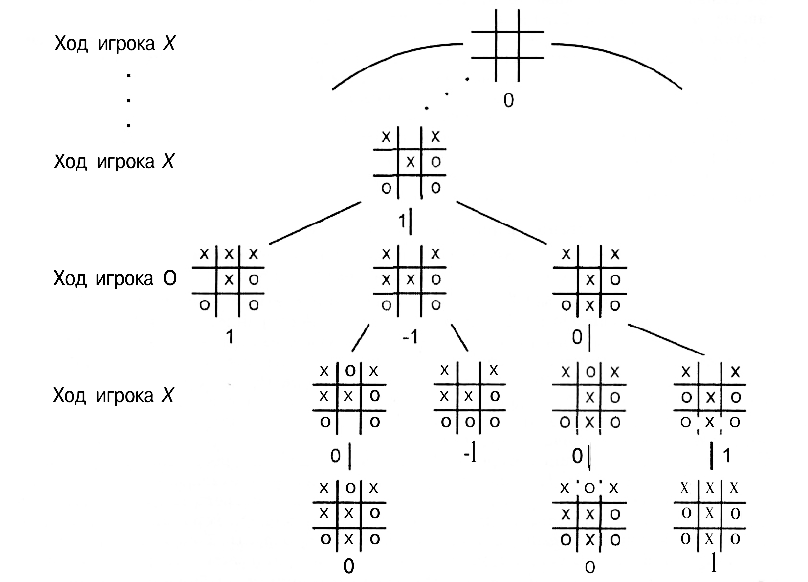
\includegraphics[scale=0.7]{xo.png}
\end{figure}
\begin{center}
	Издательский дом "Вильяме"\\
	Москва»Санкт-Петербург»Киев\\
	2003
\end{center}

\newpage
\begin{flushleft} 
	ББК 32.973.26.018.$2_{R}$75\\
	A95\\
	УДК 681.3.07
\end{flushleft}

\vspace{1cm}

\begin{center} 
	Издательский дом "Вильяме" \\
	Зав. редакцией \textit{С. Н. Тригуб}
\end{center}
\begin{center} 
	Перевод с английского и редакция канд. \textit{физ.-мат. наук А. А. Минько}
\end{center}
\begin{center} 
	По общим вопросам обращайтесь в Издательский дом "Вильяме"\\
	по адресу: info@williamspublishing.com, http://www.williamspublishing.com
\end{center}

\vspace{2cm}


\begin{center}
	Axo, Альфред, В., Хопкрофт, Джон, Ульман, Джеффри, Д. \\
	А95 Структуры данных и алгоритмы. : Пер. с англ. : М. : Издательский\\
	дом "Вильяме", 2003. — 384 с. : ил. — Парал. тит. англ.\\
	ISBN 5-8459-0122-7 (рус.)
\end{center}
В этой книге подробно рассмотрены структуры данных и алгоритмы, которые являются фундаментом современной методологии разработки программ. Показаны разнообразные реализации абстрактных типов данных, начиная от стандартных списков, стеков, очередей и заканчивая множествами и отображениями, которые используются для неформального описания и реализации алгоритмов. Две главы книги посвящены методам анализа и построения алгоритмов; приведено и исследовано множество различных алгоритмов для работы с графами, внутренней и внешней сортировки, управления памятью.

Книга не требует от читателя специальной подготовки, только предполагает его знакомство с какими-либо языками программирования высокого уровня, такими как Pascal. Вместе с тем она будет полезна специалистам по разработке программ и алгоритмов и может быть использована как учебное пособие для студентов и аспирантов, специализирующихся в области компьютерных наук.
\begin{flushright} 
	\textbf{ББК} 32.973.26.018.$2_{R}$75\\
\end{flushright}
Все названия программных продуктов являются зарегистрированными торговыми марками соответствующих фирм.

Никакая часть настоящего издания ни в каких целях не может быть воспроизведена в какой бы то ни было форме и какими бы то ни было средствами, будь то электронные или механические, включая фотокопирование и запись на магнитный носитель, если на это нет письменного разрешения издательства Addison-Wesley Publishing Company, Inc.

Rights to this book were obtained by arrangement with Addison-Wesley Longman, Inc.

Russian language edition published by Williams Publishing House according to the Agreement with R\&I Enterprises International, Copyright © 2000

Издательство выражает признательность Дмитрию Владимировичу Виленскому за информационную поддержку
\begin{flushleft} 
	ISBN 5-8459-0122-7 (рус.)\;\;\;\;\;\;\;\;\;\;\;\;\;\;\;\;\;\;\;\;\;\;\;\;\;\:© Издательский дом "Вильяме", 2000\\ 
	ISBN 0-201-00023-7 (англ.)\;\;\;\;\;\;\;\;\;\;\;\;\;\;\;\;\;\;\;\;\;\;\;\;© Addison-Wesley Publishing Company, Inc.
\end{flushleft}
\thispagestyle{empty}
\newpage
\renewcommand\contentsname{Содержание}
%\fancyfoot[RO]{\thepage}
%\fancyfoot[LO]{\textsc{СОДЕРЖАНИЕ}}
%\fancyfoot[RE]{\textsc{СОДЕРЖАНИЕ}}
%\fancyfoot[LE]{\thepage}
\thispagestyle{empty}
\begin{flushright} 
	\Huge{\textbf{Оглавление}}
\end{flushright}
%временное оглавление
\begin{table}[h]
\begin{flushleft}
{\bf \begin{tabular}{p{0.15\textwidth}p{0.65\textwidth}p{0.05\textwidth}}
ГЛАВА 1.& Построение и анализ алгоритмов & 15\\
& & \\
ГЛАВА 2.& Основные абстрактные типы данных & 45 \\ 
& & \\
ГЛАВА 3.& Деревья & 77 \\
& & \\
ГЛАВА 4.& Основные операторы множеств & 103\\
& & \\
ГЛАВА 5.& Специальные методы представления множеств & 146\\
& & \\
ГЛАВА 6.& Ориентированные графы & 183\\
& & \\
ГЛАВА 7.& Неориентированные графы & 208 \\
& & \\
ГЛАВА 8.& Сортировка & 228\\
& & \\
ГЛАВА 9.& Методы анализа алгоритмов & 265\\
& & \\
ГЛАВА 10.& Методы разработки алгоритмов & 276\\
& & \\
ГЛАВА 11.& Структуры данных и алгоритмы для внешней памяти & 311\\
& & \\
ГЛАВА 12.& Управление памятью & 339\\
& & \\
\multicolumn{2}{l}{
Список литературы} & 369
\end{tabular}}
\end{flushleft}
\end{table}


\newpage
%\thispagestyle{empty}
\tableofcontents\thispagestyle{empty}



\fancyfoot[LE]{\thepage}
\fancyfoot[RO]{\thepage}
\chapter*{Предисловие}
\thispagestyle{empty}
\addcontentsline{toc}{chapter}{Предисловие}
\fancyfoot[LO]{\textsc{ПРЕДИСЛОВИЕ}}
\fancyfoot[RE]{\textsc{ПРЕДИСЛОВИЕ}}
В этой книге описаны структуры данных и алгоритмы,\rindex{Алгоритмы} которые являются фундаментом современного компьютерного программирования. Основу данной книги составляют первые шесть глав нашей ранее изданной книги \textit{The Design and Analysis of Computer Algorithms}\footnote{Существует перевод этой книги на русский язык: Построение и анализ вычислительных алгоритмов. — М., "Мир"\ , 1979. — Прим. ред.}. Мы расширили ее содержание, включив материал по алгоритмам внешнего хранения и управлению памятью. Как и предыдущая, эта книга может составить основу учебного курса по структурам данным и алгоритмам. Мы не требуем от читателя специальной подготовки, только предполагаем его знакомство с какими-либо языками программирования высокого уровня, такими как Pascal. \rindex{Pascal}

Мы попытались осветить структуры данных и алгоритмы в более широком контексте решения задач с использованием вычислительной техники, а также использовали абстрактные типы данных для неформального описания и реализации алгоритмов. И хотя сегодня абстрактные типы данных только начинают применять в современных языках программирования, авторы считают, что они являются полезным инструментом при разработке программ независимо от применяемого языка программирования.

Мы также постоянно подчеркиваем и внедряем идею вычисления и оценки времени выполнения алгоритмов (временную сложность алгоритмов) как составную часть процесса компьютерного решения задач. В этом отражается наша надежда на то, что программисты осознают, что при решении задач прогрессирующе больших размеров особое значение имеет временная сложность выбранного алгоритма, а не возможности новых поколений вычислительных средств.

\subsection*{Представление алгоритмов}
\addcontentsline{toc}{subsection}{ Представление алгоритмов}
Мы используем язык Pascal для представления описываемых алгоритмов и структур данных просто потому, что это широко известный язык программирования. В начале книги алгоритмы часто будут представлены как в абстрактной форме, так и на языке Pascal. Это сделано для того, чтобы показать весь спектр проблем при решении практических задач: от проблемы формализации задачи до проблем, возникающих во время выполнения\rindex{Программы!время выполнения} законченной программы. Алгоритмы, которые мы представляем, можно реализовать на любых языках программирования высокого уровня.

\subsection*{Содержание книги}
\addcontentsline{toc}{subsection}{ Содержание книги}
В главе 1 содержатся вводные замечания и обсуждаются реализации процесса \textit{исходная задача — готовая программа} и роль абстрактных типов данных в этом процессе. Здесь также можно познакомиться с математическим аппаратом, необходимым для оценивания времени выполнения алгоритмов.

В главе 2 рассматриваются традиционные структуры списков, стеков и очередей, а также отображения, которые являются абстрактным типом данных, основанным на математическом понятии функции. В главе 3 вводятся деревья и основные структуры данных, которые эффективно поддерживают различные операторы, выполняемые над деревьями. 

В главах 4, 5 рассмотрено большое количество абстрактных типов данных, основанных на математической модели множеств. Достаточно глубоко исследованы словари и очереди с приоритетами\rindex{Приоритет}. Рассмотрены стандартные реализации этих абстрактных типов данных, такие как хеш-таблицы, двоичные деревья поиска, частично упорядоченные деревья, 2-3 деревья и др. Более сложный материал помещен в главу 5. 

Главы 6, 7 содержат материал, относящийся к графам; ориентированные графы рассмотрены в главе 6, а неориентированные — в главе 7. Эти главы начинают раздел книги, который больше посвящен алгоритмам, чем структурам данных, хотя мы продолжаем обсуждать основные структуры данных, подходящие для представления графов. В этих главах представлено большое количество алгоритмов для работы с графами, включая алгоритмы поиска в глубину\rindex{Поиск!в глубину}, нахождения минимального остовного дерева, кратчайших путей и максимальных паросочетаний. 

В главе 8 рассмотрены основные алгоритмы внутренней сортировки: быстрая сортировка, пирамидальная сортировка, "карманная" сортировка, а также более простые (и менее эффективные) методы, например метод сортировки вставками. В конце главы описаны алгоритмы с линейным временем выполнения для нахождения медиан и других порядковых статистик.

В главе 9 обсуждаются асимптотические методы анализа рекурсивных программ. Здесь, конечно же, рассмотрены методы решения рекуррентных соотношении. 

В главе 10 сравнительно кратко (без глубокого анализа) рассмотрены методы разработки алгоритмов, включая методы декомпозиции, динамическое программирование, алгоритмы локального поиска, и различные формы организации деревьев поиска. 

Последние две главы посвящены организации внешнего хранения и управлению памятью. Глава 11 охватывает методы внешней сортировки и организацию внешнего хранения данных, включая В-деревья и индексные структуры. 

Материал по управлению памятью, содержащийся в главе 12, условно можно разбить на четыре части, в зависимости от того, являются ли блоки памяти фиксированной или переменной длины, а также от того, явно или неявно осуществляется очистка памяти. 

Материал этой книги авторы использовали в программе лекционных курсов по структурам данным и алгоритмам в Колумбийском, Корнеллском и Станфордском университетах как для студентов, так и для аспирантов. Например, предварительную версию этой книги использовали в Станфордском университете как основу 10недельного курса по структурам данных для студентов первого года обучения. Этот курс включал материал глав 1-4, 9, 10, 12 и частично из глав 5-7. 
\subsection*{Упражнения} 
\addcontentsline{toc}{subsection}{ Упражнения}
В конце каждой главы приведено много упражнений различной степени сложности. С помощью многих из них можно просто проверить усвоение изложенного материала. Некоторые упражнения требуют дополнительных усилий и размышлений, они помечены одной звездочкой. Упражнения, помеченные двумя звездочками, рассчитаны на студентов старших курсов и аспирантов. Библиографические примечания в конце каждой главы предлагают ссылки на дополнительную литературу.
\fancyfoot[LO]{ПРЕДИСЛОВИЕ}

\newpage
\subsection*{Благодарности}
\addcontentsline{toc}{subsection}{ Благодарности}

Мы хотим выразить благодарность компании Bell Laboratories за предоставление превосходных коммуникационных средств и средств подготовки текстов (основанных на UNIX™), которые позволили легко подготовить рукопись географически разделенным авторам. Многие наши коллеги, прочитав различные части рукописи, сделали ценные замечания. Особенно мы хотим поблагодарить за полезные предложения Эда Бекхама (Ed Beckham), Джона Бентли (Jon Bentley), Кеннета Чу (Kenneth Chu), Джанет Кореи (Janet Coursey), Хенка Кокса (Hank Сох), Нейла Иммермана (Neil Immerman), Брайана Кернигана (Brian Kernighan), Стива Мехени (Steve Mahaney), Крейга Мак-Мюррей (Craig McMurray), Альберто Мендельзона (Alberto Mendelzon), Элистер Моффат (Alistair Moffat), Джеффа Нотона (Jeff Naughton), Керри Нимовичер (Kerry Nemovicher), Пола Ниэмки (Paul Niamkey), Ёшио Оно (Yoshio Ohno), Роба Пайка (Rob Pike), Криса Руэна (Chris Rouen), Мориса Шлумбергера (Maurice Schlumberger), Стенли Селкова (Stanley Selkow), Ченгай Ши (Chengya Shih), Боба Тарьяна (Bob Tarjan), В. Ван Снайдера (W. Van Snyder), Питера Вейнбергера (Peter Weinberger) и Энтони Ерёкериса (Anthony Yeracaris). Наконец, мы хотим принести огромную благодарность г-же Клейр Мецгер (Claire Metzger) за профессиональную помощь при подготовке рукописи к печати.

\begin{flushright} 
	A.V.A.\\
	J.E.H.\\
	J.D.U.\\
\end{flushright}
\chapter[Построение и анализ алгоритмов]{Построение\\ и анализ\\ алгоритмов}
\thispagestyle{empty}
\noindentПроцесс создания компьютерной программы для решения какой-либо практической задачи состоит из нескольких этапов: формализация \rindex{Алгоритмы!формализация} и создание технического задания на исходную задачу; разработка алгоритма решения задачи; написание, тестирование, отладка и документирование программы; получение решения исходной задачи путем выполнения законченной программы, В данной главе мы покажем подходы к реализации этих этапов, а в последующих рассмотрим алгоритмы и структуры данных как строительные блоки создаваемых компьютерных программ.
\section{От задачи к программе}

Половина дела сделана, если знать, что исходная задача имеет решение. В первом приближении большинство задач, встречающихся на практике, не имеют четкого и однозначного описания. Определенные задачи, такие как разработка рецепта вечной молодости или сохранение мира во всем мире, вообще невозможно сформулировать в терминах, допускающих компьютерное решение. Даже если мы предполагаем, что наша задача может быть решена на компьютере, обычно для ее формального описания требуется огромное количество разнообразных параметров. И часто только в ходе дополнительных экспериментов можно найти интервалы изменения этих параметров.

Если определенные аспекты решаемой задачи можно выразить в терминах какой-либо формальной модели, то это, безусловно, необходимо сделать, так как в этом случае в рамках формальной модели мы можем узнать, существуют ли методы и алгоритмы решения нашей задачи. Даже если такие методы и алгоритмы не существуют на сегодняшний день, то привлечение средств и свойств формальной модели поможет в построении "подходящего" решения исходной задачи.

Практически любую область математики или других наук можно привлечь к построению модели определенного круга задач. Для задач, числовых по своей природе, можно построить модели на основе общих математических конструкций, таких как системы линейных уравнений (например, для задач расчета электрических цепей или напряжений в закрепленных балках), дифференциальные уравнения (задачи прогноза роста популяций или расчета скорости протекания химических реакций). Для задач с символьными или текстовыми данными можно применить модели символьных последовательностей или формальных грамматик. Решение таких задач содержит этапы компиляции (преобразование программ, написанных на языке высокого уровня, в программы на машинноориентированных языках) и информационного поиска (распознавание определенных слов в списках заголовков каких-либо библиотек и т.п.).

\subsection*{Алгоритмы}
\addcontentsline{toc}{subsection}{ Алгоритмы}
Когда построена (подобрана) подходящая модель исходной задачи, то естественно искать решение в терминах этой модели. На этом этапе основная цель заключается в построении решения в форме алгоритма, состоящего из конечной последовательности инструкций, каждая из которых имеет четкий смысл и может быть выполнена с конечными вычислительными затратами за конечное время. Целочисленный оператор присваивания \textit{х := у + z} — пример инструкции, которая будет выполнена с конечными вычислительными затратами. Инструкции могут выполняться в алгоритме любое число раз, при этом они сами определяют число повторений. Однако мы требуем, чтобы при любых входных данных алгоритм завершился после выполнения конечного числа инструкций. Таким образом, программа, написанная на основе разработанного алгоритма, при любых начальных данных никогда не должна приводить к бесконечным циклическим вычислениям. 

Есть ещё один аспект определения алгоритмов, о котором необходимо сказать. Выше мы говорили, что алгоритмические инструкции должны иметь "четкий смысл" и выполняться с "конечными вычислительными затратами". Естественно, то, что понятно одному человеку и имеет для него "четкий смысл", может совершенно иначе представляться: другому. То же самое можно сказать о понятии "конечных затрат": на практике часто трудно доказать, что при любых исходных данных, выполнение последовательности инструкций завершится, даже если мы четко понимаем смысл каждой инструкции. В этой ситуации, учитывая все аргументы за и против, было бы полезно попытаться достигнуть соглашения о "конечных затратах" в отношении последовательности инструкций, составляющих алгоритм. Однако кажущаяся сложность подобных доказательств может быть обманчивой. В разделе 1.5 мы оценим\rindex{Время выполнения!измерение} время выполнения основных структур языков программирования, что докажет конечность времени их выполнения и соответственно конечность вычислительных затрат». 

Кроме программ на языке Pascal, мы часто будем представлять алгоритмы с помощью псевдоязыка \textit{Псевдоязык} программирования, который комбинирует обычные конструкции языков программирования с выражениями на "человеческом" языке. Мы используем Pascal как язык программирования, но практически любой другой язык программирования может быть использован вместо него для представления алгоритмов, рассматриваемых в этой книге. 

Следующие примеры иллюстрируют основные этапы создания компьютерной программы. 

Пример 1.1. Рассмотрим математическую модель, используемую для управления светофорами на сложном перекрестке дорог. Мы должны создать программу, которая в качестве входных данных использует множество всех допустимых поворотов на перекрестке (продолжение прямой дороги, проходящей через перекресток, также будем считать "поворотом") и разбивает это множество на несколько групп так, чтобы все повороты в группе могли выполняться одновременно, не создавая проблем друг для друга. Затем мы сопоставим с каждой группой поворотов соответствующий режим работы светофоров на перекрестке. Желательно минимизировать число разбиений исходного множества поворотов, поскольку при этом минимизируется количество режимов работы светофоров на перекрестке.

Для примера на рис. 1.1 показан перекресток возле Принстонского университета, известный сложностью его преодоления. Обратите внимание, что дороги \textsl{С} и \textsl{£} односторонние, остальные — двухсторонние. Всего на этом перекрестке возможно 13 поворотов. Некоторые-из этих поворотов, такие как \textsl{АВ} (поворот с дороги \textsl{А} на дорогу \textsl{В}) и \textsl{ЕС}, могут выполняться одновременно. Трассы других поворотов, например \textsl{АО} и \textsl{ЕВ}, пересекаются, поэтому их нельзя выполнять одновременно. Режимы работы светофоров должны учитывать эти обстоятельства и не допускать одновременного выполнения таких поворотов, как \textsl{AD} и \textsl{ЕВ}, но могут разрешать совместное выполнение поворотов, подобных \textsl{АВ} и \textsl{ЕС}.

\fancyfoot[RE]{ГЛАВА 1. ПОСТРОЕНИЕ И АНАЛИЗ АЛГОРИТМОВ}
\newpage
\begin{figure}[ht]
	\center{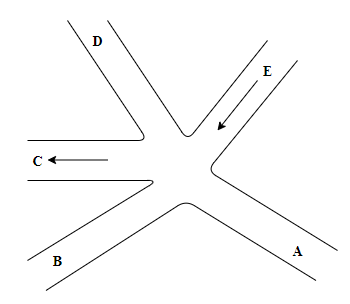
\includegraphics[scale=0.4]{1}}
	\caption{Сложный перекресток}
\end{figure}
Для построения модели этой задачи можно применить математическую структуру, известную как\rindex{Граф!ребро} граф. \textit{Граф} состоит из множества точек, которые называются\rindex{Граф!вершина} \textit{вершинами}\rindex{Вершина!графа}, и совокупности линий \textit{(ребер)}\rindex{Ребро!графа}, соединяющих эти точки. Для решения задачи управления движением по перекрестку можно нарисовать граф, где вершины будут представлять повороты, а ребра соединят ту часть вершин-поворотов, которые нельзя выполнить одновременно. Для нашего перекрестка (рис. 1.1) соответствующий граф показан на рис. 1.2, а в табл. 1.1 дано другое\rindex{Граф!представления} представление графа — в виде таблицы, где на пересечении строки \textsl{i} и столбца \textsl{j} стоит 1 тогда и только тогда, когда существует\rindex{Граф!ребро} ребро между вершинами \textsl{i} и \textsl{j}.
\begin{figure}[ht]
	\center{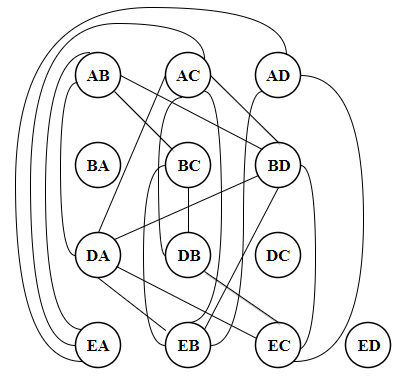
\includegraphics[scale=0.4]{2}}
	\caption{Граф, показывающий несовместимые повороты}
\end{figure}

Модель в виде графа поможет в решении исходной задачи управления светофорами. В рамках этой модели можно использовать решение, которое дает математическая задача\rindex{Граф!задача раскраски} \textit{раскраски графа}\rindex{Задача!раскраски графа} \rindex{Алгоритм!раскраски графа}\rindex{Раскраска графа}: каждой вершине графа надо так задать цвет, чтобы никакие две соединенные ребром вершины не имели одинаковый цвет, и при этом по возможности использовать минимальное количество цветов. Нетрудно видеть, что при такой раскраске графа несовместимым поворотам будут соответствовать вершины, окрашенные в разные цвета. 

Проблема раскраски графа изучается математиками уже несколько десятилетий, но теория алгоритмов мало что может сказать о решении этой проблемы. К сожалению, задача раскраски произвольного графа минимальным количеством
\fancyfoot[LO]{1.1 ОТ ЗАДАЧИ К ПРОГРАММЕ}

\newpage
\noindentцветов принадлежит классу задач, которые называются \textit{NP-полными задачами} и для которых все известные решения относятся к типу "проверь все возможности" или "перебери все варианты". Для раскраски графа это означает, что сначала для закраски вершин используется один цвет, затем — два цвета, потом — три и т.д., пока не будет получена подходящая раскраска вершин. В некоторых частных случаях можно предложить более быстрое решение, но в общем случае не существует более эффективного (в значительной степени) алгоритма решения задачи раскраски, чем алгоритм полного перебора возможных вариантов.
\begin{table}[ht]
	\caption{Таблица не совместимых поворотов}
	\begin{center}
		\begin{tabular}{c|c|c|c|c|c|c|c|c|c|c|c|c|c|}
			& AB & AC & AD & BA & BC & BD & DA & DB & DC & EA & EB & EC & ED \\
			\hline
			&  &  &  &  &  &  &  &  &  &  &  &  &  \\
			AB &  &  &  &  & 1 & 1 & 1 &  &  & 1 &  &  & \\
			AC &  &  &  &  &  & 1 & 1 & 1 &  & 1 & 1 &  & \\
			AD &  &  &  &  &  &  &  &  &  & 1 & 1 & 1 & \\
			BA &  &  &  &  &  &  &  &  &  &  &  &  & \\
			BC & 1 &  &  &  &  &  &  & 1 &  &  & 1 &  &  \\
			BD & 1 & 1 &  &  &  &  & 1 &  &  &  & 1 & 1 &  \\
			DA & 1 & 1 &  &  &  & 1 &  &  &  &  & 1 & 1 &  \\
			DB &  & 1 &  &  & 1 &  &  &  &  &  &  & 1 & \\
			DC &  &  &  &  &  &  &  &  &  &  &  &  & \\
			EA & 1 & 1 & 1 &  &  &  &  &  &  &  &  &  &  \\
			EB &  & 1 & 1 &  & 1 & 1 & 1 &  &  &  &  &  & \\
			EC &  &  & 1 &  &  & 1 & 1 & 1 &  &  &  &  & \\
			ED &  &  &  &  &  &  &  &  &  &  &  &  & \\
			\hline
		\end{tabular}
	\end{center}
\end{table}

Таким образом, поиск оптимального решения задачи раскраски графа требует больших вычислительных затрат. В этой ситуации можно воспользоваться одним из следующих трех подходов. Если граф небольшой, можно попытаться найти оптимальное решение, перебрав все возможные варианты раскраски. Однако этот подход не приемлем для больших графов, так как программно трудно организовать эффективный перебор всех вариантов. Второй подход предполагает использование дополнительной информации об исходной задаче. Желательно найти какие-то особые свойства графа, которые исключали бы необходимость полного перебора всех вариантов раскраски для нахождения оптимального решения. В третьем подходе мы немного изменяем постановку задачи и ищем не оптимальное решение, а близкое к оптимальному. Если мы откажемся от требования минимального количества цветов раскраски графа, то можно построить алгоритмы раскраски, которые работают значительно быстрее, чем алгоритмы полного перебора. Алгоритмы, которые быстро находят "подходящее", но не оптимальное решение, называются \textit{эвристическими}.

Примером рационального эвристического алгоритма может служить следующий "жадный" \rindex{Алгоритм!жадный} алгоритм раскраски графа. В этом алгоритме сначала мы пытаемся раскрасить как можно больше вершин в один цвет, затем закрашиваем во второй цвет также по возможности максимальное число оставшихся вершин, и т.д. При закраске вершин в новый цвет мы выполняем следующие действия.

\begin{enumerate}
	\item Выбираем произвольную незакрашенную вершину и назначаем ей новый цвет.
	
	\item Просматриваем список незакрашенных вершин и для каждой из них определяем, соединена ли она ребром с вершиной, уже закрашенной в новый цвет. Если не соединена, то к этой вершине также применяется новый цвет.
\end{enumerate}

\newpage
Этот алгоритм назван "жадным" из-за того, что каждый цвет применяется к максимально большому числу вершин, без возможности пропуска некоторых из них или перекраски ранее закрашенных. Возможны ситуации, когда, будь алгоритм менее "жадным" и пропустил бы некоторые вершины при закраске новым цветом, мы получили бы раскраску графа меньшим количеством цветов. Например, для раскраски графа на рис. 1.3 можно было бы применить два цвета, закрасив вершину 1 в красный цвет, а затем, пропустив вершину 2, закрасить в красный цвет вершины 3 и 4. Но "жадный" алгоритм, основываясь на порядковой очередности вершин, закрасит в красный цвет вершины 1 и 2, для закраски остальных вершин потребуются еще два цвета.
\begin{figure}[ht]
	\centering
	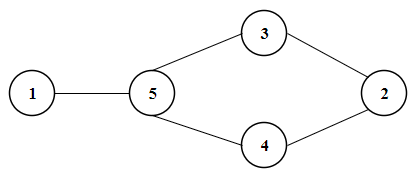
\includegraphics[scale=0.4]{3}
	\caption{Граф}
\end{figure}
Применим описанный алгоритм для закраски вершин графа нашей задачи (рис.1.2), при этом первой закрасим вершину \textsl{АВ} в синий цвет. Также можно закрасить в синий цвет вершины \textsl{AC}, \textsl{AD} и \textsl{ВА}, поскольку никакие из этих четырех вершин не имеют общих ребер. Вершину \textsl{ВС} нельзя закрасить в этот цвет, так как существует ребро между вершинами \textsl{АВ} и \textsl{ВС}. По этой же причине мы не можем закрасить в синий цвет вершины \textsl{BD}, \textsl{DA} и \textsl{DB} — все они имеют хотя бы по одному ребру, связывающему их с уже закрашенными в синий цвет вершинами. Продолжая перебор вершин, закрашиваем вершины \textsl{DC} и \textsl{ED} в синий цвет, а вершины \textsl{ЕА}, \textsl{ЕВ} и \textsl{ЕС} оставляем незакрашенными.

Теперь применим второй цвет, например красный. Закраску этим цветом начнем с вершины \textsl{ВС}. Вершину \textsl{BD} можно закрасить красным цветом, вершину \textsl{DA} — нельзя, так как есть ребро между вершинами \textsl{BD} и \textsl{DA}. Продолжаем перебор вершин: вершину \textsl{DB} нельзя закрасить красным цветом, вершина \textsl{DC} уже закрашена синим цветом, а вершину \textsl{ЕА} можно закрасить красным. Остальные незакрашенные вершины имеют общие ребра с вершинами, окрашенными в красный цвет, поэтому к ним нельзя применить этот цвет.

Рассмотрим незакрашенные вершины \textsl{DA}, \textsl{DB}, \textsl{ЕВ} и \textsl{ЕС}. Если вершину \textsl{DA} мы закрасим в зеленый цвет, то в этот цвет также можно закрасить и вершину \textsl{DB}, но вершины \textsl{ЕВ} и \textsl{ЕС} в зеленый цвет закрасить нельзя. К последним двум вершинам применим четвертый цвет, скажем, желтый. Назначенные вершинам цвета приведены в табл. 1.2. В этой таблице "дополнительные" повороты совместимы с соответствующими поворотами из столбца "Повороты", хотя алгоритмом они окрашены в разные цвета. При задании режимов работы светофоров, основанных на одном из цветов раскраски, вполне безопасно включить в эти режимы и дополнительные повороты.

Данный алгоритм не всегда использует минимально возможное число цветов. Можно использовать результаты из общей теории графов для оценки качества полученного решения. В теории графов\rindex{Граф!k-клика} \textit{k-кликой}\rindex{k-клика} называется множество из \textit{k} вершин, в котором каждая пара вершин соединена ребром. Очевидно, что для закраски fe-клики необходимо \textit{k} цветов, поскольку в клике никакие две вершины не могут иметь одинаковый цвет.
\fancyfoot[LO]{ОТ ЗАДАЧИ К ПРОГРАММЕ}

\newpage
\begin{table}[ht]
	\caption{ Раскраска графа, представленного на рис 1.2}
	\begin{center}
		\begin{tabular}{c|c|c}
			Цвет& Повороты & Дополнительные повороты \\
			\hline
			&  &  \\
			Синий & \textsl{AB,AC,AD,BA,DC,ED} & --- \\
			Красный & \textsl{BC,BD,EA} & \textsl{BA,OC,ED} \\
			Зеленый & \textsl{DA,DB} & \textsl{AD,BA,DC,ED} \\
			Желтый & \textsl{EB,EC} & \textsl{BA,DC,EA,ED} \\
			
			\hline
		\end{tabular}
	\end{center}
\end{table}

B графе рис. 1.2 множество из четырех вершин \textsl{AC, DA, BD} и \textsl{ЕВ} является 4-кликой. Поэтому не существует раскраски этого графа тремя и менее цветами, и, следовательно, решение; -представленное в табл. 1.2 является оптимальным в том смысле, что иснользует минимально возможное количество цветов для раскраски графа. В терминах исходной задачи это означает, что для управления перекрестком, доказанным на рис. 1.1, необходимо не менее четырех режимов работы светофоров.

Итак, для управления перекрестком построены четыре режима работы светофорами, которые соответствуют четырем цветам раскраски графа (табл. 1.2).$\square$

\subsection*{Псевдоязык и пошаговая "кристаллизация" алгоритмов}
\addcontentsline{toc}{subsection}{ Псевдоязык и пошаговая "кристаллизация" алгоритмов}
Поскольку для решения исходной задачи мы применяем некую математическую модель, то тем самым мржно формализовать алгоритм решения в терминах этой модели. В начальных версиях алгоритма часто применяются обобщенные операторы, которые затем переопределяются в виде более мелких, четко определенных инструкций. Например, при описании рассмотренного выше алгоритма раскраски графа мы использовали такие выражения, как "выбрать произвольную незакрашенную вершину". Мы надеемся, что читателю совершенно ясно, как надо понимать такие инструкции. Но для преобразования таких неформальных алгоритмов в компьютерные программы необходимо пройти через несколько этапов формализации (этот процесс можно назвать \textit{пошаговой кристаллизацией}), пока мы не получим программу, полностью состоящую из формальных операторов языка программирования.

Пример 1.2. Рассмотрим процесс преобразования "жадного" алгоритма раскраски графа в программу на языке Pascal. Мы предполагаем, что есть граф \textsl{G}, вершины которого необходимо раскрасить. Программа \textit{greedy}\rindex{Программа!greedy} (жадный) определяет множество вершин, названное \textit{newclr} (новый цвет), все вершины которого можно окрасить в новый цвет. Эта программа будет вызываться на повторное выполнение столько раз, сколько необходимо для закраски всех вершин исходного графа. В самом первом грубом приближении программа \textit{greedy} на псевдоязыке показана в следующем листинге.

\begin{lstlisting}[language=C, caption={Первое приближение программы \textit{greedy}}, numbers=none]
    void greedy (\textbf{GRAPH} *G, \textbf{SET} *newclr){
        /*| greedy присваивает переменной newclr множество вершин |
	                | графа G, которые можно окрасить в один цвет |*/
	    newclr = 0; /*| в данном контексте 0|
	                  | означает пустое множество |*/
	    for(|для каждой незакрашенной вершины $v$ из $G$|){
		    if(|$v$ не соединена с вершинами из $newclr$|){
		    	|пометить $v$ цветом;|
		    	|добавить $v$ в $newclr$;|
		    }
	    }
    }/* greedy */
\end{lstlisting}

\fancyfoot[RE]{ГЛАВА 1. ПОСТРОЕНИЕ И АНАЛИЗ АЛГОРИТМОВ}

\newpage

В листинге 1.1 вы легко выделите средства нашего псевдоязыка. Мы применяем полужирное начертание для зарезервированных ключевых слов языка Pascal, которые имеют тот же смысл, что и в стандартном языке Pascal. Написание строчными буквами таких слов, как GRAPH (Граф) и SET\footnote{Мы отличаем абстрактный тип данных \rindex{Абстрактный тип данных} \rindex{Абстрактный тип данных!SET} \rindex{Абстрактный тип данных!GRAPH} SET от встроенного типа данных set языка Pascal.} (Множество), указывает на имена \textit{абстрактных типов данных}. Их можно определить с помощью объявления типов языка Pascal и операторов, соответствующих абстрактным типам данных, которые задаются посредством процедур языка Pascal (эти процедуры должны входить в окончательный вариант программы). Более детально абстрактные типы данных мы рассмотрим в следующих двух разделах этой главы.

Управляющие конструкции языка Pascal, такие как if, for и while, могут применяться в операторах псевдоязыка, но условные выражения в них (как в строке (6)) могут быть неформальными, в отличие от строгих логических выражений Си. Также и в строке (4) в правой части оператора присваивания применяется неформальный символ. Еще отметим, что оператор цикла for в строке (5) проводит повторные вычисления по элементам множества.

Чтобы стать исполняемой, программа на псевдоязыке должна быть преобразована в программу на языке Си. В данном случае мы не будем приводить все этапы такого преобразования, а покажем только пример преобразования оператора if (строка (6)) в более традиционный код.

Чтобы определить, имеет ли вершина \textit{v} соединение с какой-либо вершиной из \textit{newclr}, мы рассмотрим каждый элемент \textit{w} из \textit{newclr} и по графу \textsl{G} проверим, существует ли ребро между вершинами \textit{v} и \textit{w}. Для этого используем новую булеву переменную \textit{found} (поиск), которая будет принимать значение \textit{true} (истина), если такое ребро существует. Листинг 1.2 показывает частично преобразованную программу листинга 1.1.
\begin{lstlisting}[language=C, numbers=none, caption={Частично преобразованная программа \textit{greedy}}]
    void greedy (\textbf{GRAPH} *G, \textbf{SET} *newclr){
	    newclr = 0; /* | в данном контексте |
	                   | 0 означает пустое множество| */
	    for(|для каждой незакрашенной вершины $v$ из $G$|){
		    found = false;
		    for (|для каждой вершины $w$ из $newclr$|)
			    if(|существует ребро между $v$ и $w$|)
				    found = true;
    		if(found == false){
	    		/*| $v$ не соединена с вершинами из $newclr$ |*/
		    	|пометить $v$ цветом|;
			    |добавить $v$ в $newclr$|;
		    }
	    }
    }/* |greedy| */
\end{lstlisting}
\fancyfoot[LO]{ОТ ЗАДАЧИ К ПРОГРАММЕ}

Обратите внимание, что наш алгоритм работает с двумя множествами вершин. Внешний цикл (строки (3) - (15)) выполняется над множеством незакрашенных вершин графа \textsl{G}. Внутренний цикл (строки (5) - (8)) работает с текущим множеством вершин \textit{newclr}. Оператор строки (13) добавляет новые вершины в это множество.

Существуют различные способы представления множеств в языках программирования. В главах 4 и 5 мы изучим несколько таких представлений. В этом примере мы можем представить каждое множество вершин посредством абстрактного типа LIST \rindex{LIST} (Список)\rindex{Список} \rindex{Абстрактный тип данных!LIST}, который можно выполнить в виде обычного списка целых чисел, ограниченного специальным значением \textit{null} (для обозначения которого мы будем использовать число 0). Эти целые числа могут храниться, например, в массиве, но есть и другие способы представления данных типа LIST, которые мы рассмотрим в главе 2.

\newpage
Теперь можно записать оператор for в строке (5) в виде стандартного цикла ло условию, где переменная \textit{w} инициализируется как первый элемент списка \textit{newclr} и затем при каждом выполнении цикла принимает значение следующего элемента из \textit{newclr}. Мы также преобразуем оператор for строки (3) листинга 1.1. Измененная процедура \textit{greedy} представлена в листинге 1.3. В этом листинге есть еще операторы, которые необходимо преобразовать в стандартный код языка Си, но мы пока ограничимся сделанным.
\begin{lstlisting}[language=C, numbers=none, caption={Изменения программы \textit{greedy}}]
    void greedy (|\textbf{GRAPH}| *G, |\textbf{SET}| *newclr){
	/*| greedy присваивает переменной $newclr$ множество вершин|
	            | графа $G$, которые можно окрасить в один цвет |*/
	|\textbf{bool}| found;
	int v, w;
	newclr = 0; /*| в данном контексте 0 |
	                | означает пустое множество |*/
    	while(v != NULL){
	    	found = false;
    		w = |первая вершина из $newclr$|;
    		while(w != NULL){
    			if(|существует ребро между $v$ и $w$|){
    				found = true;
    			}
    			w = |следующая вершина из $newclr$|;
    		}
    		if(found == false){
    			/*| $v$ не соединена с вершинами из $newclr$ |*/
    			|пометить $v$ цветом|;
    			|добавить $v$ в $newclr$|;
    		}
    		v = |следующая незакрашенная вершина из $G$|;
    	}
    }/* greedy */
\end{lstlisting}
\subsection*{Резюме}
\addcontentsline{toc}{subsection}{ Резюме}

На рис. 1.4 схематически представлен процесс программирования так, как он трактуется в этой книге. На первом этапе создается модель исходной задачи, для чего привлекаются соответствующие подходящие математические модели (такие как теория графов в предыдущем примере). На этом этапе для нахождения решения также строится неформальный алгоритм.

На следующем этапе алгоритм записывается на псевдоязыке — композиции (смеси) конструкций языка Pascal и менее формальных и обобщенных операторов на простом "человеческом" языке. Продолжением этого этапа является замена неформальных операторов последовательностью более детальных и формальных операторов. С этой точки зрения программа на псевдоязыке должна быть достаточно подробной, так как в ней фиксируются (определяются) различные типы данных, над которыми выполняются операторы. Затем создаются абстрактные типы данных для каждого зафиксированного типа данных (за исключением элементарных типов данных, таких как целые и действительные числа или символьные строки) путем задания имен процедурам для каждого оператора, выполняемого над данными абстрактного типа, и замены их (операторов) вызовом соответствующих процедур.

Третий этап процесса программирования обеспечивает реализацию каждого абстрактного типа данных и создание процедур для выполнения различных операторов над данными этих типов. На этом этапе также заменяются все неформальные операторы
\fancyfoot[RE]{ГЛАВА 1. ПОСТРОЕНИЕ И АНАЛИЗ АЛГОРИТМОВ}

\newpage
\noindentпсевдоязыка на код языка Pascal. Результатом этого этапа должна быть выполняемая программа. После ее отладки вы получите работающую программу, и мы надеемся, что, используя пошаговый подход при разработке программ, схема которого показана на рис. 1.4, процесс отладки конечной программы будет небольшим и безболезненным.
\begin{figure}[ht]
\centering
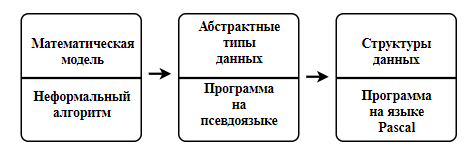
\includegraphics[scale=0.4]{4}
\caption{Схема процесса создания программ для решения прикладных задач}
\end{figure}
\section{Абстрактные типы данных}\rindex{Тип данных}
Большинство понятий, введенных в предыдущем разделе, обычно излагаются в начальном курсе программирования и должны быть знакомы читателю. Новыми могут быть только абстрактные типы данных, поэтому сначала обсудим их роль в процессе разработки программ. Прежде всего сравним абстрактный тип данных с таким знакомым понятием, как процедура.

Процедуру, неотъемлемый инструмент программирования, можно рассматривать как обобщенное понятие оператора. В отличие от ограниченных по своим возможностям встроенных операторов языка программирования (сложения, умножения и т.п.), с помощью процедур программист может создавать собственные операторы и применять их к операндам различных типов, не только базовым. Примером такой процедурыоператора может служить стандартная подпрограмма перемножения матриц.

Другим преимуществом процедур (кроме способности создавать новые операторы) является возможность использования их для \textit{инкапсулирования} частей алгоритма путем помещения в отдельный раздел программы всех операторов, отвечающих за определенный аспект функционирования программы. Пример инкапсуляции: использование одной процедуры для чтения входных данных любого типа и проверки их корректности. Преимущество инкапсуляции заключается в том, что мы знаем, какие инкапсулированные операторы необходимо изменить в случае возникновения проблем в функционировании программы. Например, если необходимо организовать проверку входных данных на положительность значений, следует изменить только несколько строк кода, и мы точно знаем, где эти строки находятся.

\subsection*{Определение абстрактного типа данных}
\addcontentsline{toc}{subsection}{ Определение абстрактного типа данных}

Мы определяем \textit{абстрактный тип данных} (АТД) как математическую модель с совокупностью операторов, определенных в рамках этой модели. Простым примером АТД могут служить множества целых чисел с операторами объединения, пересечения и разности множеств. В модели АТД операторы могут иметь операндами не только данные, определенные АТД, но и данные других типов: стандартных типов языка программирования или определенных в других АТД. Результат действия оператора также может иметь тип, отличный от определенных в данной модели АТД. Но мы предполагаем, что по крайней мене один операнд или результат любого оператора имеет тип данных, определенный в рассматриваемой модели АТД.

Две характерные особенности процедур — обобщение и инкапсуляция\rindex{Инкапсуляция}, — о которых говорилось выше, отлично характеризуют абстрактные типы данных. АТД можно рассматривать как обобщение простых типов данных (целых и действительных чисел и т.д.), точно так же, как процедура является обобщением простых операторов (+, - и т.д.). АТД инкапсулирует типы данных в том смысле, что определение типа и
\fancyfoot[LO]{1.2. АБСТРАКТНЫЕ ТИПЫ ДАННЫХ}

\newpage
\noindentвсе операторы, выполняемые над данными этого типа, помещаются в один раздел программы. Если необходимо изменить реализацию АТД, мы знаем, где найти и что изменить в одном небольшом разделе программы, и можем быть уверенными, что это не приведет к ошибкам где-либо в программе при работе с этим типом данных. Более того, вне раздела с определением операторов АТД мы можем рассматривать типы АТД как первичные типы, так как объявление типов формально не связано с их реализацией. Но в этом случае могут возникнуть сложности, так как некоторые операторы могут инициироваться для более одного АТД и ссылки на эти операторы должны быть в разделах нескольких АТД.

Для иллюстрации основных идей, приводящих к созданию АТД, рассмотрим процедуру \textit{greedy} из предыдущего раздела (листинг 1.3), которая использует простые операторы над данными абстрактного типа LIST (список целых чисел). Эти операторы должны выполнить над переменной \textit{newclr} типа LIST следующие действия.
\begin{enumerate} 
\item Сделать список пустым. 
\item Выбрать первый элемент списка и, если список пустой, возвратить значение \textit{null}. 
\item Выбрать следующий элемент списка и возвратить значение \textit{null}, если следующего элемента нет. 
\item Вставить целое число в список.
\end{enumerate}

Возможно применение различных структур данных, с помощью которых можно эффективно выполнить описанные действия. (Подробно структуры данных будут рассмотрены в главе 2.) Если в листинге 1.3 заменить соответствующие операторы выражениями.
\rindex{Оператор!NEXT}
\rindex{Оператор!INSERT}
\begin{flushleft}
MAKENULL(\textit{newcfr}); \\
\textit{w} := FIRST(\textit{newclr}); \\
\textit{w} := NEXT(\textit{newclr}); \\
INSERT(\textit{u, newclr}); \\
\end{flushleft} 
\noindent то будет понятен один из основных аспектов (и преимуществ) абстрактных типов данных. Можно реализовать тип данных любым способом, а программы, использующие объекты этого типа, не зависят от способа реализации типа — за это отвечают процедуры, реализующие операторы для этого типа данных. 

Вернемся к абстрактному типу данных GRAPH (Граф). Для объектов этого типа необходимы операторы, которые выполняют следующие действия.
\begin{enumerate}
\item Выбирают первую незакрашенную вершину. 
\item Проверяют, существует ли ребро между двумя вершинами. 
\item Помечают вершину цветом. 
\item Выбирают следующую незакрашенную вершину.
\end{enumerate}

Очевидно, что вне поля зрения процедуры \textit{greedy} остаются и другие операторы, такие как вставка вершин и ребер в граф или помечающие все вершины графа как незакрашенные. Различные структуры данных, поддерживающие этот тип данных, будут рассмотрены в главах 6 и 7.

Необходимо особо подчеркнуть, что количество операторов, применяемых к объектам данной математической модели, не ограничено. Каждый набор операторов определяет отдельный АТД. Вот примеры операторов, которые можно определить для абстрактного типа данных SET (Множество).
\begin{enumerate}
\item MAKENULL\rindex{Оператор!MAKENULL}(\textsl{A}). Эта процедура делает множество \textsl{А} пустым множеством. 
\item UNION\rindex{Оператор!UNION}(\textsl{A, В, С}). Эта процедура имеет два "входных" аргумента, множества \textsl{А} и \textsl{В}, и присваивает объединение этих множеств "выходному" аргументу — множеству \textsl{С}. 
\item SIZE\rindex{Оператор!SIZE}(\textsl{A}). Эта функция имеет аргумент-множество \textsl{А} и возвращает объект целого типа, равный количеству элементов множества \textsl{А}.
\end{enumerate}
\fancyfoot[RE]{ГЛАВА 1. ПОСТРОЕНИЕ И АНАЛИЗ АЛГОРИТМОВ}

\newpage

Термин  \textit{реализация} АТД подразумевает следующее: перевод в операторы языка
программирования объявлений, определяющие переменные этого абстрактного типа
данных, плюс процедуры для каждого оператора, выполняемого над объектами АТД.
Реализация зависит от \textit{структуры данных}\rindex{Структуры данных}, представляющих АТД. Каждая структура
данных строится на основе базовых типов данных применяемого языка программирования,
используя доступные в этом языке средства структурирования данных.
Структуры массивов и записей — два важных средства структурирования данных,
возможных в языке Си. Например, одной из возможных реализаций переменной
S типа SET может служить массив, содержащий элементы множества S.

Одной из основных причин определения двух различных АТД в рамках одной модели
является то, что над объектами этих АТД необходимо выполнять различные
действия, т.е. определять операторы разных типов. В этой книге рассматривается
только несколько основных математических моделей, таких как теория множеств и
теория графов, но при различных реализациях на основе этих моделей определенных
АТД будут строиться различные наборы операторов.

В идеале желательно писать программы на языке, базовых типов данных и операторов
которого достаточно для реализации АТД. С этой точки зрения язык Си не
очень подходящий язык для реализации различных АТД, но, с другой стороны,
трудно найти иной язык программирования, в котором можно было бы так непосредственно
декларировать АТД. Дополнительную информацию о таких языках программирования
см. в библиографических примечаниях в конце главы.

\section{Типы данных, структуры данных и абстрактные типы данных}

\fancyfoot[LO]{1.3. ТИПЫ ДАННЫХ, СТРУКТУРЫ ДАННЫХ И АБСТРАКТНЫЕ ТИПЫ ДАННЫХ}
Хотя термины \textit{тип данных} (или просто \textit{тип}), \textit{структура данных} и \textit{абстрактный
тип данных} звучат похоже, но имеют они различный смысл. В языках программирования
\textit{тип данных} переменной обозначает множество значений, которые
может принимать эта переменная. Например, переменная булевого (логического) типа
может принимать только два значения: значение true (истина) и значение false
(ложь) и никакие другие. Набор базовых типов данных отличается в различных языках:
в языке Си это типы целых (int) и действительных (float, double) чисел, булев
(bool) тип %%(отсутствует в Си до версии С99, в которой определен как _Bool и в заголовочном файле bool.h имеет указанный псевдоним)
и символьный (char) тип. Правила конструирования составных типов
данных (на основе базовых типов) также различаются в разных языках программирования:
как мы уже упоминали, Си легко и быстро строит такие типы.

Абстрактный тип данных — это математическая модель плюс различные операторы,
определенные в рамках этой модели. Как уже указывалось, мы можем разрабатывать
алгоритм в терминах АТД, но для реализации алгоритма в конкретном
языке программирования необходимо найти способ представления АТД в терминах
типов данных и операторов, поддерживаемых данным языком программирования.
Для представления АТД используются \textit{структуры данных}, которые представляют
собой набор переменных, возможно, различных типов данных, объединенных определенным
образом.

Базовым строительным блоком структуры данных является ячейка \rindex{Ячейка}, которая
предназначена для хранения значения определенного базового или составного типа
данных. Структуры данных создаются путем задания имен совокупностям
(агрегатам) ячеек и (необязательно) интерпретации значения некоторых ячеек как
представителей (т.е. указателей) других ячеек.

В качестве простейшего механизма агрегирования ячеек в Си и большинстве
других языков программирования можно применять (одномерный) массив, т.е. последовательность
ячеек определенного типа. Массив также можно рассматривать как
отображение множества индексов (таких как целые числа 0, 1, ..., $n$) в множество
ячеек. Ссылка на ячейку обычно состоит из имени массива и значения из множества
индексов данного массива. Значения всех ячеек массива должны иметь одинаковый тип данных.
В Си множество индексов не может быть нечислового типа (как например, в Pascal'е). 
% Нечто похожее можно сделать с символьным и перечисляемым типами т.к. в Си они хорошо ... .
Объявление
\begin{lstlisting}[numbers=none]
	|\textbf{Тип\_Ячеек} имя[]|;
\end{lstlisting}
задает имя для последовательности ячеек, тип для элементов множества индексов и
тип содержимого ячеек.

Многие языки программирования, как и Си, позволяют использовать в качестве индексов только множества последовательных
целых чисел. Например, чтобы в языке Fortran в качестве индексов массива
можно было использовать буквы, надо все равно использовать целые индексы, заменяя
"А"{}  на 1, "В"{}  на 2, и т.д.

Другим общим механизмом агрегирования ячеек в языках программирования является
\textit{структура записи}. \textit{Запись} (record) можно рассматривать как ячейку, состоящую
из нескольких других ячеек (называемых \textit{полями}), значения в которых могут
быть разных типов. Записи часто группируются в массивы; тип данных определяется
совокупностью типов полей записи. Например, в Си объявление
\begin{lstlisting}[numbers=none]
    struct structName{
    	float data;
    	int next;
    }
    struct structName reelist[4];
\end{lstlisting}

задает имя \textit{reclist} (список записей) 4-элементного массива, значениями которого являются
записи с двумя полями: data (данные) и next (следующий).

Третий метод агрегирования ячеек, который можно найти в Си и некоторых
других языках программирования, — это \textit{файл} \rindex{Файл}. Файл, как и одномерный массив,
является последовательностью значений определенного типа. Однако файл не имеет
индексов: его элементы доступны только в том порядке, в каком они были записаны
в файл. В отличие от файла, массивы и записи являются структурами с
"произвольным доступом"{}, подразумевая под этим, что время доступа к компонентам
массива или записи не зависит от значения индекса массива или указателя поля записи.
Достоинство агрегирования с помощью файла (частично компенсирующее описанный
недостаток) заключается в том, что файл не имеет ограничения на количество
составляющих его элементов и это количество может изменяться во время выполнения
программы.

\subsection*{Указатели и курсоры}
\addcontentsline{toc}{subsection}{ Указатели и курсоры}
В дополнение к средствам агрегирования ячеек в языках программирования
можно использовать указатели и курсоры.  \textit{Указатель}\rindex{Указатель} (pointer) — это ячейка, чье
значение указывает на другую ячейку. При графическом представлении структуры
данных в виде схемы тот факт, что ячейка А является указателем на ячейку В, показывается
с помощью стрелки от ячейки А к ячейке В.
В языке Си с помощью следующего объявления можно создать переменную-указатель
$prt$, указывающую на ячейку определенного типа, например ТипЯчейки:
\begin{lstlisting}[numbers=none]
    |\textbf{ТипЯчейки} *prt|; 
\end{lstlisting}
Префикс $*$ в Си используется как оператор
разыменования, т.е. выражение \verb|*prt| обозначает значение (типа ТипЯчейки) в ячейке,
указанной  \textit{prt}.

\textit{Курсор} (cursor) — это ячейка с целочисленным значением, используемая для указания
на массив. В качестве способа указания курсор работает так же, как и указатель,
но курсор можно Использовать и в языках (подобных Fortran), которые не
имеют явного типа указателя. Интерпретировав целочисленную ячейку как индексное 
значение для массива, можно эффективно реализовать указания на ячейки массива.
К сожалению, этот прием подходит только для ячеек массива и не позволяет
организовать указание на ячейки, не являющиеся частью массива.

В схемах структур данных мы будем рисовать стрелку из ячейки курсора к ячейке,
на которую указывает курсор. Иногда мы также будем показывать целое число в
ячейке курсора, напоминая тем самым, что это не настоящий указатель.
Языки программирования, подобные PL/I или С, позволяют компонентам массивов
быть истинными указателями и, конечно, "быть указанным"{} с помощью курсора. В
отличие от этих языков, в языках Fortran и Algol, где нет типа указателя, можно
использовать только курсоры.

Пример 1.3. На рис. 1.5 показана структура данных, состоящая из двух частей.
Она имеет цепочку ячеек, содержащих курсоры для массива \textit{reclist} (список записей),
определенного выше. Назначение поля \textit{next} (следующий) заключается в указании на
следующую запись в массиве \textit{reclist}. Например, \textit{reclist}[4].\textit{next} равно 1, поэтому запись
4 предшествует записи 1. Полагая первой запись 4, в соответствии со значениями
поля \textit{next} получим следующий порядок записей: 4, 1, 3, 2. Отметим, что значение
поля \textit{next} в записи 2, равное 0, указывает на то, что нет следующей записи. Целесообразно
принять соглашение, что число 0 будет обозначать \textit{нуль-указатель} при
использовании курсоров и указателей. Но, чтобы не возникали проблемы при реализации
этого соглашения, необходимо также \textit{условиться}, что массивы, на которые
указывают курсоры, индексируются начиная с 1, а не с 0.
\begin{figure}[ht]
	\centering
	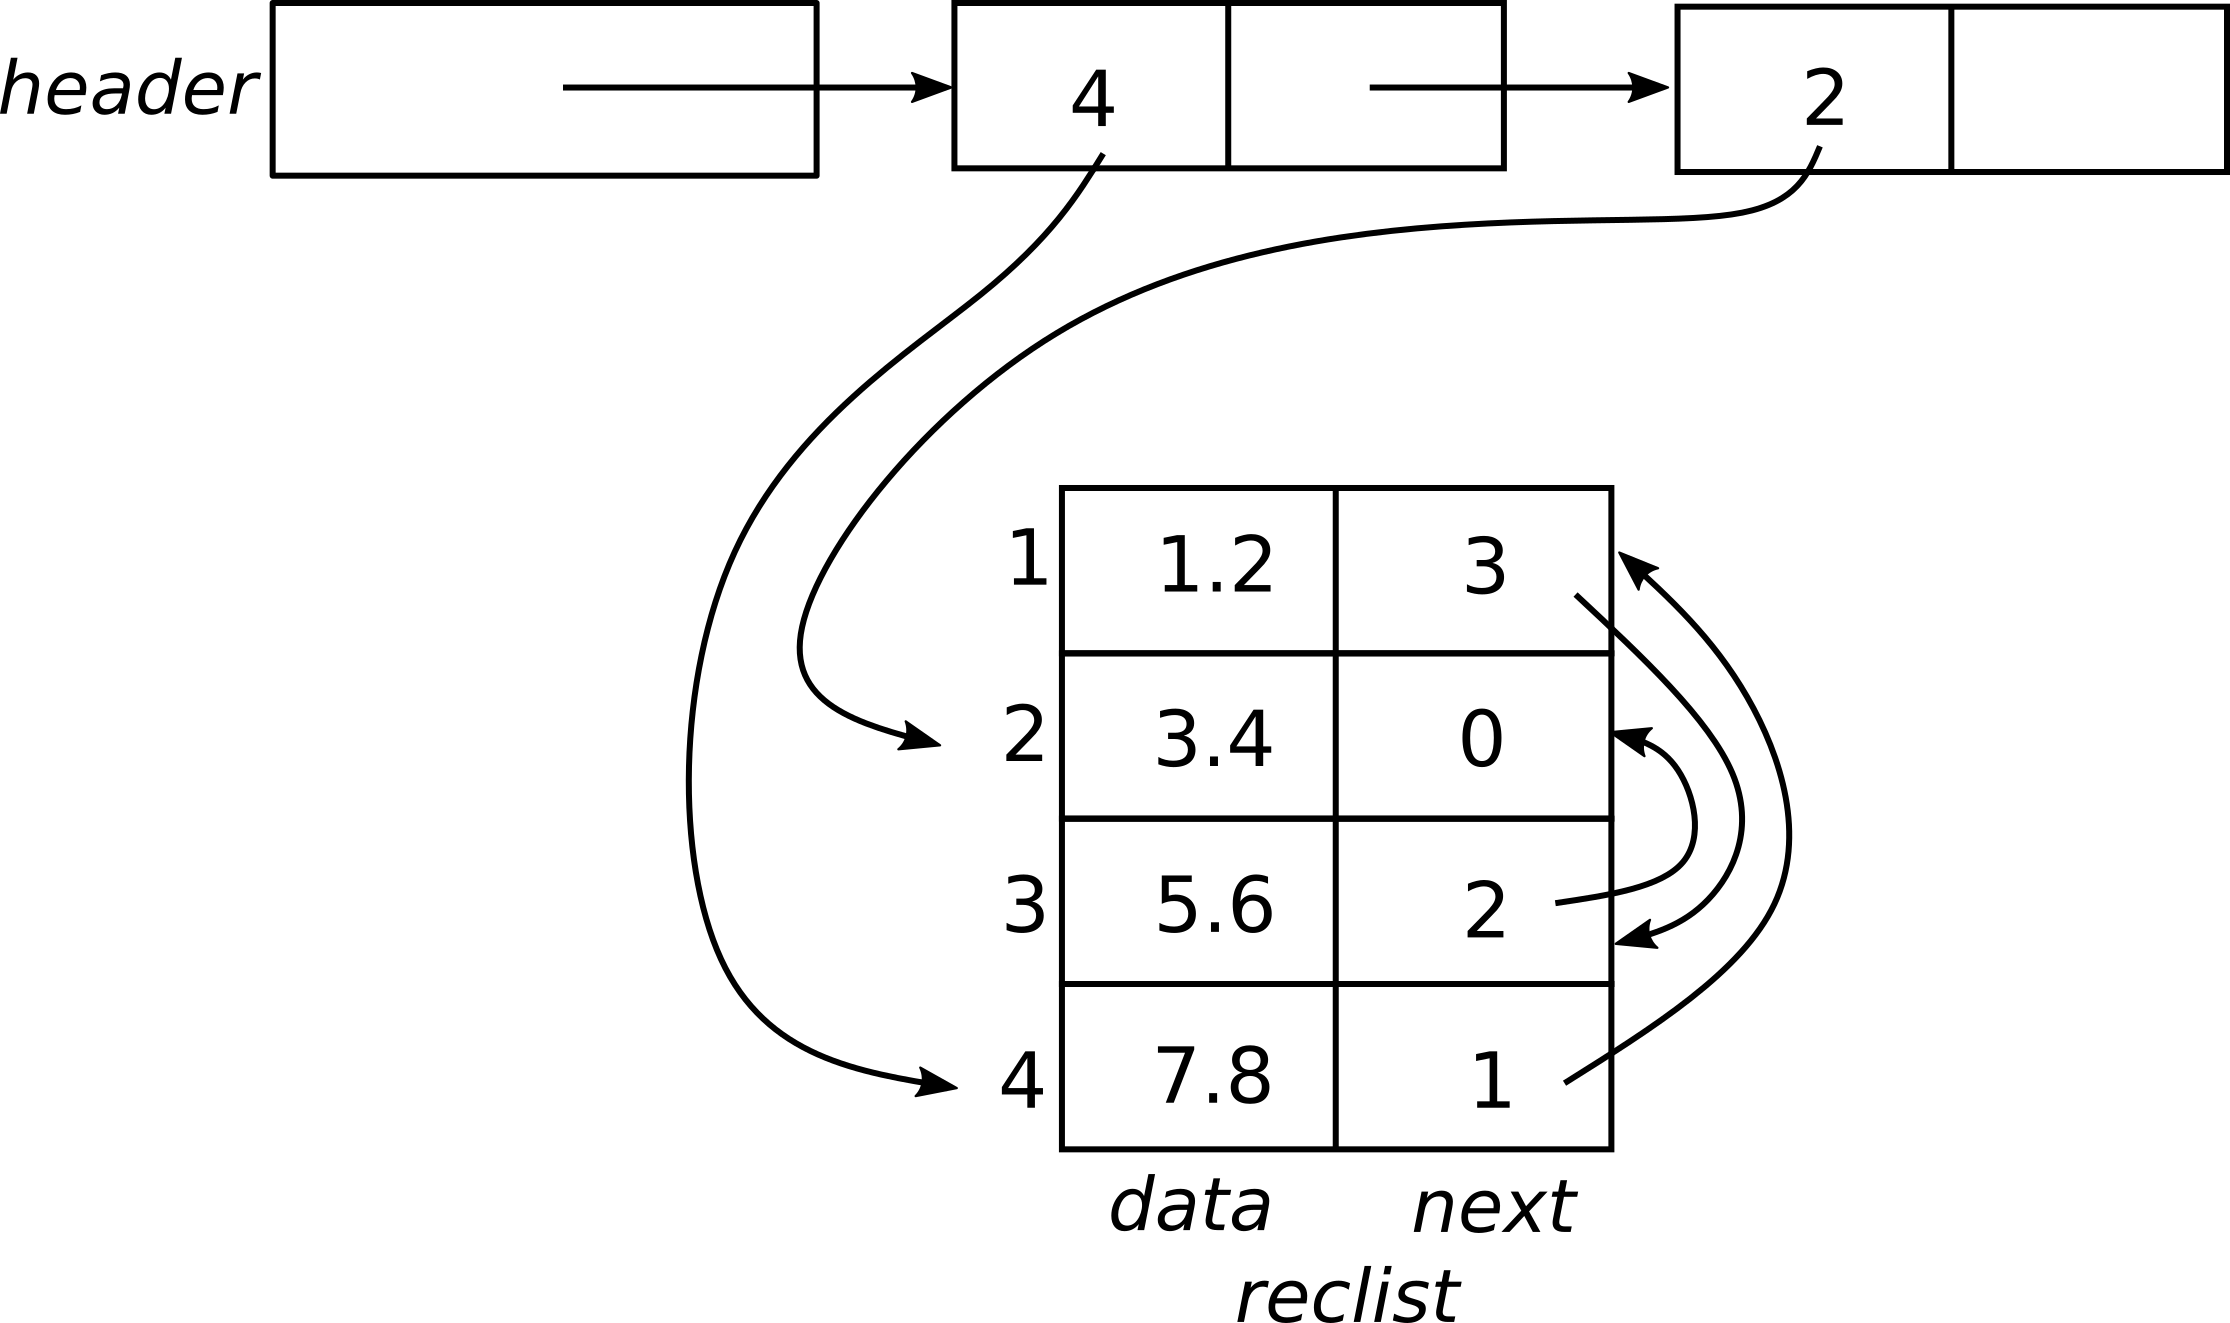
\includegraphics[width=\textwidth]{pictures/27}
	\caption{Пример структуры данных}
\end{figure}

Ячейки в цепочке на рис. 1.5 имеют тип
\begin{lstlisting}[language=C, numbers=none]
    typedef struct Trecordtype{
    	int cursor;
    	\textbf{Trecordtype} ptr;
    } recordtype;
\end{lstlisting}
На цепочку можно ссылаться с помощью переменной \textit{header} (заголовок), имеющей
тип recordtype, \textit{header} указывает на анонимную запись типа recordtype\footnote[1]{ Запись анонимна (не имеет имени), так как создается с помощью вызова  \textit{new}(\textit{header}), где
 \textit{header} указывает на вновь создаваемую запись. В памяти компьютера, конечно, есть адрес, по
которому можно локализовать ячейку с записью.}.Эта запись имеет значение 4 в поле cursor. Мы рассматриваем 4 как индекс массива
realist. Эта запись имеет истинный указатель в поле ptr на другую анонимную
запись, которая, в свою очередь, указывает на индекс 4 массива reclist и
имеет нуль-указатель в поле prt.

\section{Время выполнения программ}
\fancyfoot[LO]{ 1.4. ВРЕМЯ ВЫПОЛНЕНИЯ ПРОГРАММ}
В процессе решения прикладных задач выбор подходящего алгоритма вызывает
определенные трудности. В самом деле, на чем основывать свой выбор, если алгоритм
должен удовлетворять следующим противоречащим друг другу требованиям.

\begin{enumerate}[topsep=0pt,itemsep=1ex,partopsep=1ex,parsep=1ex]
\item Быть простым для понимания, перевода в программный код и отладки.
\item Эффективно использовать компьютерные ресурсы и выполняться по возможности
быстро.
\end {enumerate}

Если написанная программа должна выполняться только несколько раз, то первое
требование наиболее важно. Стоимость рабочего времени программиста обычно значительно
превышает стоимость машинного времени выполнения программы, поэтому
стоимость программы оптимизируется по стоимости написания (а не выполнения) программы.
Если мы имеем дело с задачей, решение которой требует значительных вычислительных
затрат, то стоимость выполнения программы может превысить стоимость
написания программы, особенно если программа должна выполняться многократно.
Поэтому, с финансовой точки зрения, более предпочтительным может стать
сложный комплексный алгоритм (в надежде, что результирующая программа будет
выполняться существенно быстрее, чем более простая программа). Но и в этой ситуации
разумнее сначала реализовать простой алгоритм, чтобы определить, как должна
себя вести более сложная программа. При построении сложной программной системы
желательно реализовать ее простой прототип, на котором можно провести необходимые
измерения и смоделировать ее поведение в целом, прежде чем приступать к разработке
окончательного варианта. Таким образом, программисты должны быть осведомлены не
только о методах построения быстрых программ, но и знать, когда их следует применить
(желательно с минимальными программистскими усилиями).

\subsection*{Измерение времени выполнения программ}
\addcontentsline{toc}{subsection}{ Измерение времени выполнения программ}

На время выполнения программы влияют следующие факторы.

\begin{enumerate}[topsep=0pt,itemsep=1ex,partopsep=1ex,parsep=1ex]
\item Ввод исходной информации в программу.
\item Качество скомпилированного кода исполняемой программы.
\item Машинные инструкции (естественные и ускоряющие), используемые для выполнения
программы.

\item Временная сложность алгоритма соответствующей программы\footnote[1]{Здесь авторы, не акцентируя на этом внимания и не определяя его особо, вводят термин
"временная сложность алгоритма"{}. Под \textit{временной сложностью алгоритма} понимается "время"{}
выполнения алгоритма, измеряемое в "шагах"{} (инструкциях алгоритма), которые необходимо выполнить
алгоритму для достижения запланированного результата. В качестве синонима для
этого термина авторы часто используют выражение "время выполнения алгоритма"{}. Отметим,
что в первой части книги (до главы 6) авторами чаще используется последнее выражение, а во
второй — чаще термин\rindex{Временная сложность} "временная сложность"{}. В этой связи заметим, что необходимо различать
"время выполнения алгоритма"{} и "время выполнения программы"{}. — \textit{Прим. ред.}
}.
\end {enumerate}

Поскольку время выполнения программы зависит от ввода исходных данных, его
можно определить как функцию от исходных данных. Но зачастую время выполнения
программы зависит не от самих исходных данных, а от их "размера"{}. В этом отношении
хорошим примером являются задачи \textit{сортировки}\rindex{Задача!сортировки}\rindex{Сортировка}, которые мы подробно
рассмотрим в главе 8. В задачах сортировки в качестве входных данных выступает
список элементов, подлежащих сортировке, а в качестве выходного результата — те
же самые элементы, отсортированные в порядке возрастания или убывания. Например,
входной список 2, 1, 3, 1, 5, 8 будет преобразован в выходной список 1, 1, 2, 3, 5, 8
(в данном случае список \textit{отсортирован в порядке возрастания}). Естественной
мерой объема входной информации для программы сортировки будет число элементов,
подлежащих сортировке, или, другими словами, длина входного списка,
В общем случае длина входных данных т- Подходящая мера объема входной информации, и если не будет оговорено иное, то в качестве меры объема входной информации
мы далее будем понимать именно длину входных данных.

Обычно говорят, что\rindex{Время выполнения!программ} время выполнения программы имеет порядок, $T(n)$ от входных
данных размера $n$. Например, некая программа имеет время выполнения $T(n) = cn^2$,
где $c$ — константа. Единица измерения $T(n)$ точно не определена, но мы будем понимать
$T(n)$ как количество инструкций, выполняемых на идеализированном компыотере.

Для многих программ время выполнения действительно является функцией входных
данных, а не их размера. В этой ситуации мы определяем $T(n)$ как время выполнения
в \textit{наихудшем случае},  т.e. как максимум времени выполнения по всем входным
данным размера п. Мы также будем рассматривать $T_{cp}(n)$ как среднее (в статистическом
смысле) время выполнения по всем входным данным размера $n$. Хотя $T_{cp}(n)$ является
достаточно объективной мерой времени выполнения, но часто, нельзя предполагать
(или обосновать) равнозначность всех входных данных. На практике среднее время выполнения
найти сложнее, чем ндихудщее время выполнения, так как математически
это трудноразрешимая задача и, кроме того, зачастую не имеет простого определения
понятие "средних"{} входных данных. Поэтому в основном мы будем использовать наихудшее
время выполнения как меру временной сложности алгоритмов, но не будем за-
бывать и о среднем времени выполнения там, где это возможно,

Теперь сделаем замечание о втором и третьем факторах, влияющих на время выполнения
программ: о компиляторе, используемом для компиляции программы, и
машине, на которой выполняется программа. Эти факторы влияют на то, что для
измерения времени выполнения $T(n)$ мы не можем применить стандартные единицы
измерения, такие как секунды или миллисекунды. Поэтому мы можем только делить
заключения, подобные "время выполнения такого-то алгоритма пропорционально $n^2$"{}.
Константы пропорциональности также нельзя точно определить, поскольку они
зависят от компилятора, компьютера и других факторов.

\subsection*{Асимптотические соотношения} 
\rindex{Асимптотические соотношения}
\addcontentsline{toc}{subsection}{ Асимптотические соотношения}

Для описания скорости роста функций используется $O$-симвблйка. Например, когда
мы говорим, что время выполнения $T(n)$ некоторой программы имеет порядок $O(n^2)$
(читается "о-болыное от $n$ в квадрате"{} или просто "о от $n$ в квадрате"{}),
то подразумевается, что существуют положительные константы $c$ и $n_0$, такие, что для всех
$n$, больших или равных $n_0$, выполняется неравенство $T(n) \leq cn^2$.

\textbf{Пример 1.4.} Предположим, что $T(0)=1$, $T(1)=4$ и в общем случае $T(n)=(n+1)^2$. Тогда
$T(n)$  имеет порядок $O(n^2)$: если положить $n_0 = 1$  и $c=4$, то легко показать,
что для $n\geq1$ будет выполяться неравенство $(n+1)^2 \leq 4n^2$.
Отметим, что нельзя положить $n_0 = 0$, так как $T(0) = 1$ и, следовательно, это значение при любой константе $c$  больше $c0^2=0$. $\square$

Подчеркнем: мы предполагаем, что все функции времени выполнения опредедены
на множестве неотрицательных целых чисел и их значения также неотрицательны,
но необязательно целые. Будем говорить, что  $T(n)$ имеет порядок $O(f(n))$, если существуют константы
$c$ и $n_0$, такие, что для всех  $n \geq n_0$ выполняется неравенство $T(n)\leq cf(n)$.
Для программ, у которых время выполнения имеет порядок $O(f(n))$, говорят, что они имеют порядок (или степень) роста $f(n)$.

\textbf{Пример 1.5.} Функция $T(n)=3n^3+2n^2$ имеет степень роста $O(n^3)$. Чтобы это показать,
надо положить $n_0=0$ и $c=5$, так как легко видеть, что для всех целых $n \geq 0$ выполяется неравенство $3n^3+2n^2 \leq 5n^3$.
Можно, конечно, сказать, что $T(n)$ имеет порядок роста $O(n^4)$, но это более слабое утверждение, чем то, что $T(n)$ имеет порядок роста $O(n^3)$.

В качестве следующего примера докажем, что функция $3^n$ не может иметь порядок $O(2^n)$.
Предположим, что существуют константы $c$ и $n_0$ такие, что для всех $n \geq n_0$ выполняется неравенство
$3^n \leq c2^n$. Тогда $c \geq (3/2)^n$ для всех $n \geq n_0$. Но $(3/2)^n$ принимает
любое, как %сколь???
угодно большое, значение при достаточно большом $n$, поэтому не
существует такой константы $c$, которая могла бы мажорировать $(3/2)^n$ для всех $n$. $\square$

Когда мы говорим, что $T(n)$ имеет степень роста $O(f(n))$, то подразумевается, что $f(n)$ является верхней границей скорости роста $T(n)$.
Чтобы указать нижнюю границу скорости роста $T(n)$, используется обозначение: $T(n)$ есть $\Omega(g(n))$
(читается "омега-большое от $g(n)$"{} или просто "омега от $g(n)$"{}), это подразумевает существование такой константы $c$,
что бесконечно часто (для бесконечного числа значений $n$) выполняется неравенство $T(n) \geq cg(n)$.\footnote[1]{Отметим асимметрию
в определениях $O$- и $\Omega$-символики. Такая асимметрия бывает полезной,
когда алгоритм работает быстро на достаточно большом подмножестве, но не на всем
множестве входных данных. Например, есть алгоритмы, которые работают значительно быстрее,
если длина входных данных является простым числом, а не (к примеру) четным числом.
В этом случае невозможно получить хорошую нижнюю границу времени выполнения,
справедливую для всех $n \geq n_0$}

\textbf{Пример 1.6.} Для проверки того, что $T(n)=n^3+2n^2$ есть $\Omega(n^3)$, достаточно положить $c=1$.
Тогда $T(n) \geq cn^3)$ для $n=0, 1, \dots$\ .

Для другого примера положим, что $T(n)=n$ для нечетных $n\geq1$ и $T(n)=n^2/100$ —
для четных $n \geq 0$. Для доказательства того, что $T(n)$ есть $\Omega(n^2)$, достаточно положить $c=1/100$
и рассмотреть множество четных чисел  $n=0, 2, 4, 6, \dots$\ . $\square$

\subsection*{Ограниченность показателя степени роста}
\addcontentsline{toc}{subsection}{ Ограниченность показателя степени роста}

Итак, мы предполагаем, что программы можно оценить с помощью функций времени
выполнения, Пренебрегая при этом константами пропорциональности. С этой
точки зрения программа с временем выполнения $O(n^2)$, например, лучше программы
с временем выполнения $O(n)$. Константы пропорциональности зависят не только от
используемых компилятора и компьютера, но и от свойств самой программы. Пусть
при определенной комбинации компилятор-компьютер одна программа выполняется
за $100n^2$ миллисекунд, а вторая — за $5n^3$ миллисекунд. Может ли вторая программа
быть предпочтительнее, чем первая?

Ответ на этот вопрос зависит от размера входных данных программ. При размере
входных данных $n < 20$ программа с временем выполнения $5n^3$ завершится быстрее,
чем программа с временем выполнения $100n^2$. Поэтому, если программы в основном
выполняются с входными данными небольшого размера, предпочтение необходимо
отдать программе с временем выполнения $O(n^3)$. Однако при возрастании $n$ 
отношение времени выполнения $5n^3/100n^2 = n/20$ также растет. Поэтому при больших $n$
программа с временем выполнения $O(n^2)$ становится предпочтительнее программы с
временем выполнения $O(n^3)$. Если даже при сравнительно небольших $n$, когда время
выполнения обеих программ примерно одинаково, выбор лучшей программы представляет
определенные затруднения, то естественно для большей надежности сделать
выбор в пользу программы с меньшей степенью роста.
Другая причина, заставляющая отдавать предпочтение программам с наименьшей
степенью роста времени выполнения, заключается в том, что чем меньше степень
роста, тем больше размер задачи, которую можно решить на компьютере. Другими
словами, если увеличивается скорость вычислений компьютера, то растет также и
размер задач, решаемых на компьютере. Однако незначительное увеличение скорости
вычислений компьютера приводит только к небольшому увеличению размера задач,
решаемых в течение фиксированного промежутка времени, исключением из этого
правила являются программы с низкой степенью роста, как $O(n)$ и  $O(n\log{n})$.

\textbf{Пример 1.7.} На рис. 1.6 показаны функции времени выполнения (измеренные в
секундах) для четырех программ с различной временной сложностью для одного и того же
сочетания компилятор-компьютер. Предположим, что можно использовать
1 000 секунд (примерно 17 минут) машинного времени для решения задачи. Какой
максимальный размер задачи, решаемой за это время? За 10 секунд каждый из четырех
алгоритмов может решить задачи примерно одинакового размера, как показано
во втором столбце табл. 1.3.

Предположим, что получен новый компьютер (без дополнительных финансовых
затрат), работающий в десять раз быстрее. Теперь за ту же цену можно использовать
$10^4$ секунд машинного времени — ранее $10^3$ секунд. Максимальный размер
задачи, которую может решить за это время каждая из четырех программ, показан
в третьем столбце табл. 1.3. Отношения значений третьего и второго столбцов приведены
в четвертом столбце этой таблицы. Здесь мы видим, что увеличение скорости
компьютера на 1 000\% приводит к увеличению только на 30\% размера задачи,
решаемой с помощью программы с временем выполнения $O(2^n)$.
Таким образом, 10-кратное увеличение производительности компьютера дает в процентном отношении
значительно меньший эффект увеличения размера решаемой задачи. В действительности,
независимо от быстродействия компьютера, программа с временем выполнения $O(2^n)$
может решать только очень небольшие задачи.
\begin{figure}[ht]
\centering
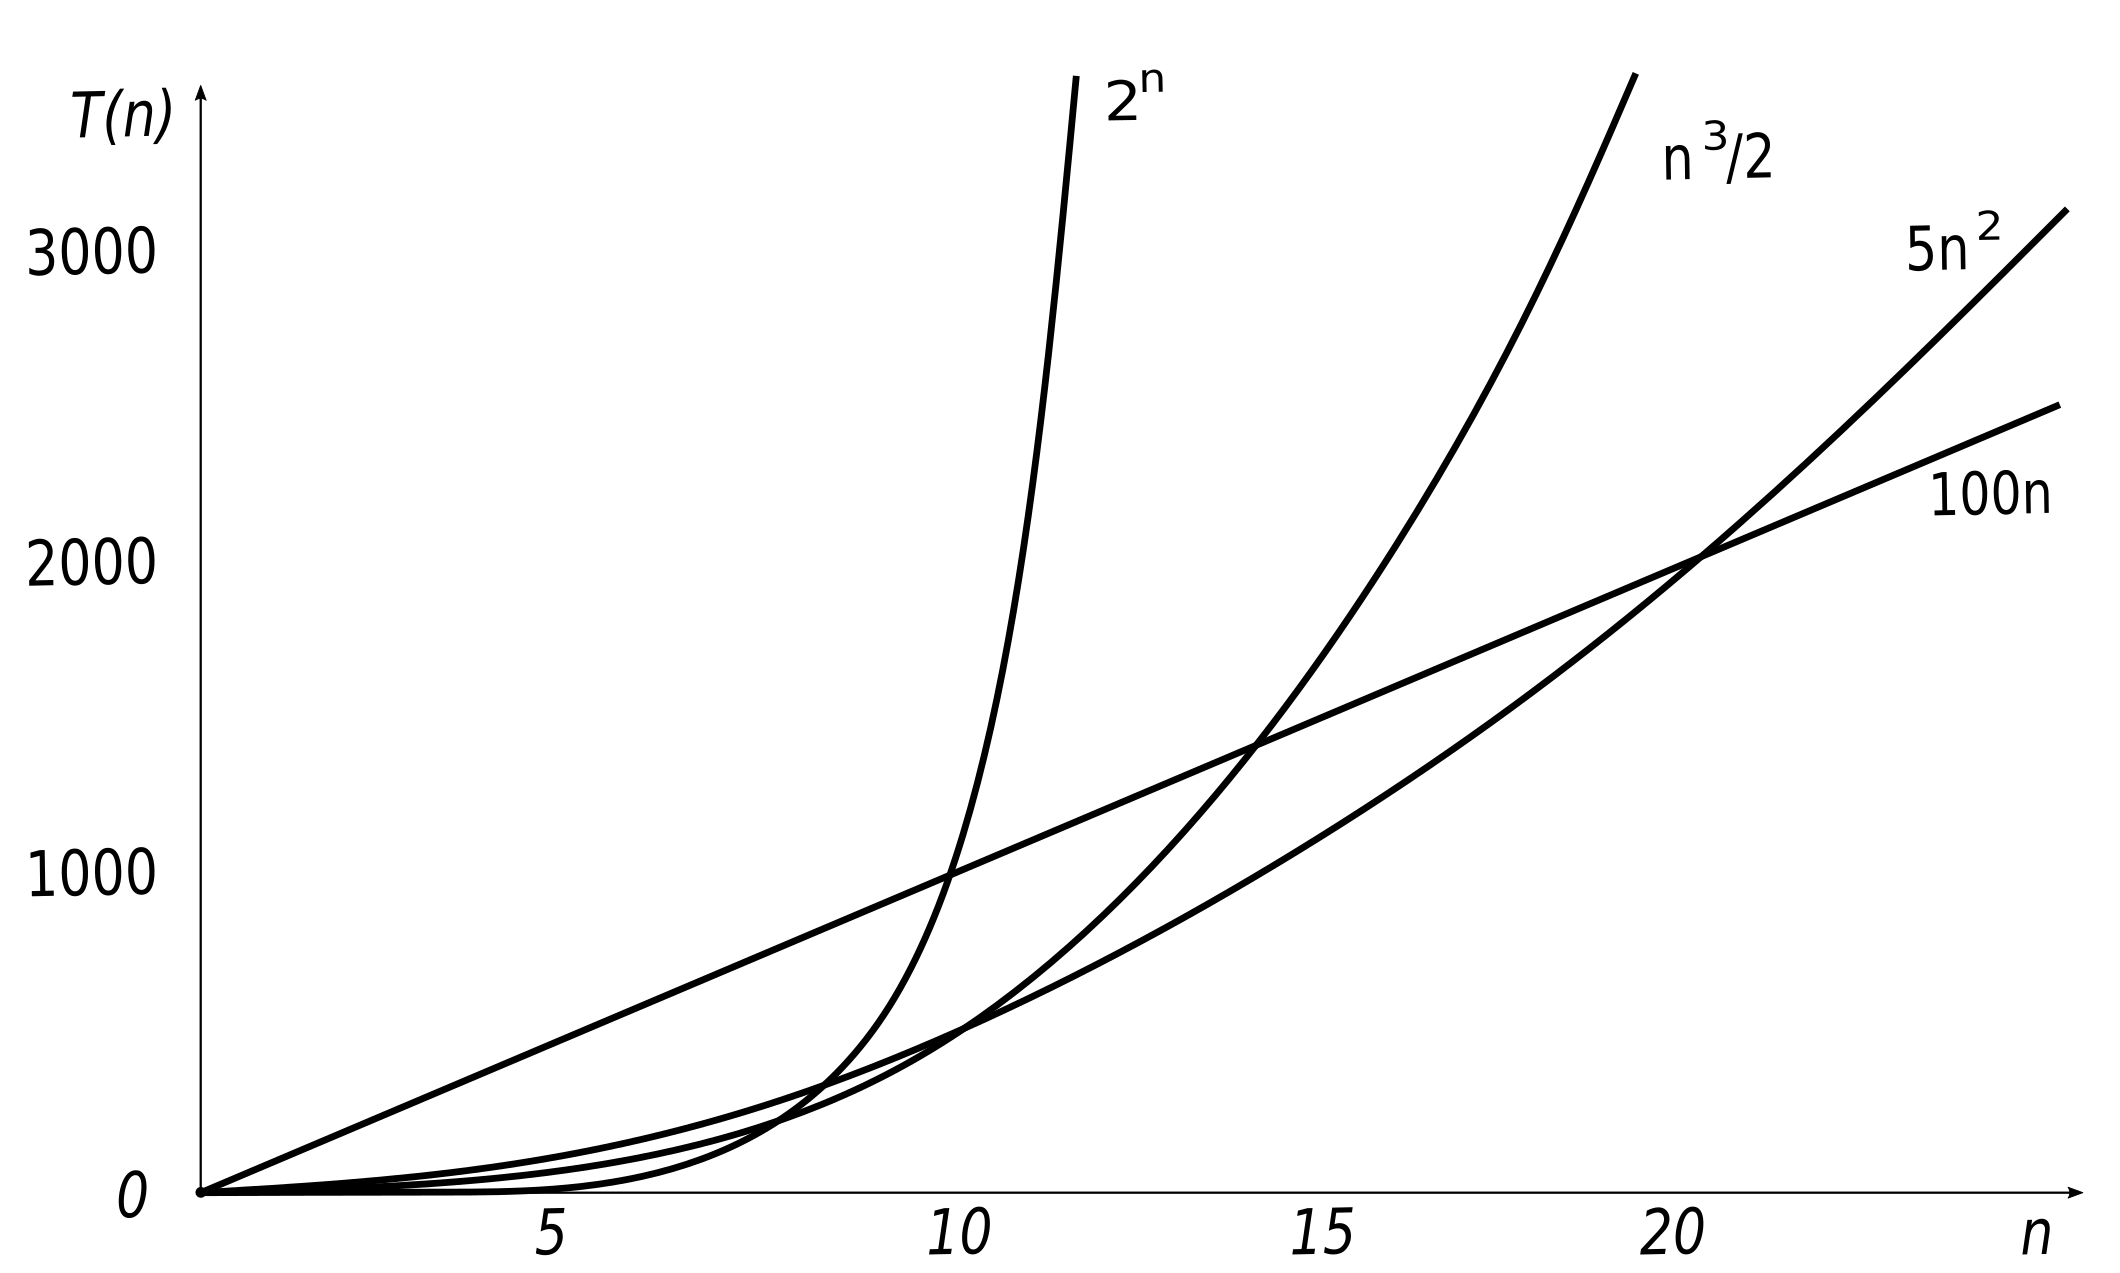
\includegraphics[width=\textwidth]{pictures/31}
\caption{\textit{Функции времени выполнения четырех программ}}
\end{figure}
\textit{Рис. 1.6 Функции времени выполнения четырех программ}\\
\begin{table}[ht]
\centering
\caption{Эффект от 10-кратного увеличения быстродействия компьютера}
\begin{tabular}{cccc}
Время  & Максимальный  & Максимальный размер  & Увеличение  \\
выполнения $T(n)$ & размер  задачи & размер  задачи & максимального\\
	& для $10^3$ секунд & для $10^4$ секунд & размера задачи\\
\hline \\[-1em]
$100n$ & 10 & 10 & 10.0\\
$5n^2$ & 14 & 45 & 3.2\\
$n^3/2$ & 12 & 27 & 2.3\\
$2^n$ & 10 & 13 & 1.3\\
\end{tabular}

\end{table}

Из третьего столбца табл. 1.3 ясно видно преимущество программ с временем выполнения $O(n)$:
10-кратное увеличение размера решаемой задачи при 10-кратном
увеличении производительности компьютера. Программы с временем выполнения  $O(n^3)$ и $O(n^2)$
при увеличении быстродействия компьютера на 1 000\% дают увеличение
размера задачи соответственно на 230\% и 320\%. Эти соотношения сохранятся и
при дальнейшем увеличении производительности компьютера.$\square$

Поскольку существует необходимость решения задач все более увеличивающегося
размера, мы приходим к почти парадоксальному выводу. Так как машинное время
все время дешевеет, а компьютеры становятся более быстродействующими, мы надеемся,
что сможем решать все большие по размеру и более сложные задачи. Но вместе
с тем возрастает значимость разработки и использования эффективных алгоритмов
именно с низкой степенью роста функции времени выполнения.

\subsection*{Немного соли}
\addcontentsline{toc}{subsection}{ Немного соли}

Мы хотим еще раз подчеркнуть, что степень роста наихудшего времени выполнения
— не единственный или самый важный критерий оценки алгоритмов и программ.
Приведем несколько соображений, позволяющих посмотреть на критерий
времени выполнения с других точек зрения.
\begin{enumerate}[topsep=0pt,itemsep=1ex,partopsep=1ex,parsep=1ex]
\item Если создаваемая программа будет использована только несколько раз, тогда
стоимость написания и отладки программы будет доминировать в общей стоимости
программы, т.е. фактическое время выполнения не окажет существенного
влияния на общую стоимость. В этом случае следует предпочесть алгоритм, наиболее
простой для реализации.
\item Если программа будет работать только с "малыми"{} входными данными, то степень
роста времени выполнения будет иметь меньшее значение, чем константа,
присутствующая в формуле времени выполнения. Вместе с тем и понятие
"малости"{} входных данных зависит от точного времени выполнения конкурирующих
алгоритмов. Существуют алгоритмы, такие как алгоритм целочисленного
умножения (см. [96]), асимптотически самые эффективные, но которые никогда
не используют на практике даже для больших задач, так как их константы
пропорциональности значительно превосходят подобные константы других, более
простых и менее "эффективных"{} алгоритмов.
\item Эффективные, но сложные алгоритмы могут быть нежелательными, если готовые
программы будут поддерживать лица, не участвующие в написании этих программ.
Будем надеяться, что принципиальные моменты технологии создания
эффективных алгоритмов широко известны, и достаточно сложные алгоритмы
свободно применяются на практике. Однако необходимо предусмотреть возможность
того, что эффективные, но "хитрые"{} алгоритмы не будут востребованы из-за
их сложности и трудностей, возникающих при попытке в них разобраться.
\item Известно несколько примеров, когда эффективные алгоритмы требуют таких
больших объемов машинной памяти (без возможности использования более медленных
внешних средств хранения), что этот фактор сводит на нет преимущество
"эффективности"{} алгоритма.
\item В численных алгоритмах точность и устойчивость алгоритмов не менее важны,
чем их временная эффективность.
\end {enumerate}

\section{Вычисление времени выполнения программ}
\fancyfoot[LO]{ 1.5. ВЫЧИСЛЕНИЕ ВРЕМЕНИ ВЫПОЛНЕНИЯ ПРОГРАММ}
Теоретическое нахождение времени выполнения программ (даже без определения
констант пропорциональности) — сложная математическая задача. Однако на практике
определение времени выполнения (также без нахождения значения констант)
является вполне разрешимой задачей — для этого нужно знать только несколько базовых
принципов. Но прежде чем представить эти принципы, рассмотрим, как выполняются
операции сложения и умножения с использованием $O$-символики.

Пусть $T_1(n)$ и $T_2(n)$ — время выполнения двух программных фрагментов  $P_1$ и $P_2$,
$T_1(n)$ имеет степень роста $O(f(n))$, а $T_2(n)$ — $O(g(n))$. Тогда $T_1(n) + T_2(n)$, т.е. время
последовательного выполнения фрагментов $P_1$ и $P_2$, имеет степень роста $O(\max(f(n), g(n)))$.
Для доказательства этого вспомним, что существуют константы $c_1$, $c_2$, $n_1$ и $n_2$, такие, что при
$n \geq n_1$ выполняется неравенство $T_1(n) \leq c_1f(n)$, и , аналогично, $T_2(n) \leq c_2g(n)$, если $n \geq n_2$.
Пусть $n_0=\max (n_1, n_2)$. Если $n \geq n_0$, то очевидо, что $T_1(n) + T_2(n) \leq c_1f(n) + c_2g(n)$. 
Отсюда вытекает, что при $n \geq n_0$ справедливо неравенство $T_1(n) + T_2(n) \leq (c_1 + c_2)\max(f(n), g(n))$.
Последнее неравенство и означает, что $T_1(n) + T_2(n)$ имеет порядок роста $O(\max(f(n), g(n)))$.

\textbf{Пример 1.8.} \textit{Правило сумм}\rindex{Правило!сумм}, данное выше, используется для вычисления времени
последовательного выполнения программных фрагментов с циклами и ветвлениями.
Пусть есть три фрагмента с временами выполнения соответственно $O(n^2)$, $O(n^3)$ и $O(n\log{n})$.
Тогда время последовательного выполнения первых двух фрагментов имеет
порядок $O(\max(n^2, n^3))$, т.е. $O(n^3)$. Время выполнения всех трех фрагментов имеет
порядок $O(\max(n^3,n\log{n}))$, это то же самое, что $O(n^3)$.$\square$

В общем случае время выполнения конечной последовательности программных
фрагментов, без учета констант, имеет порядок фрагмента с наибольшим временем выполнения.
Иногда возможна ситуация, когда порядки роста времен нескольких фрагментов
\textit{несоизмеримы} (ни один из них не больше, чем другой, но они и не равны). Для
примера рассмотрим два фрагмента с временем выполнения  $O(f(n))$ и $O(g(n))$, где
\begin{align*}
f(n)=\left\{ \begin{array}{ll} 
n^4,& \textrm{ если $n$ четное;}
\\
n^2, & \textrm{ если $n$ нечетное,}
\end{array} \right. &
g(n)=\left\{ \begin{array}{ll} 
n^2,& \textrm{ если $n$ четное;}
\\
n^3, & \textrm{ если $n$ нечетное.}
\end{array} \right.
\end{align*}

В данном случае правило сумм можно применить непосредственно и получить время
выполнения $O(\max(f(n), g(n)))$, т.е. $n^4$ при $n$ четном и $n^3$, если $n$ нечетно.

Из правила сумм также следует, что если  $g(n) \leq f(n)$ для всех $n$, превышающих $n_0$, то
выражение  $O(f(n)+g(n))$ эквивалентно $O(f(n))$. Например,  $O(n^2+n)$ то же самое, что $O(n^2)$.

\textit{Правило произведений}\rindex{Правило!произведений} заключается в следующем. Если $T_1(n)$ и $T_2(n)$ имеют степени роста
$O(f(n))$ и $O(g(n))$ соответственно, то произведение $T_1(n)T_2(n)$ имеет степень
роста $O(f(n)g(n))$. Читатель может самостоятельно доказать это утверждение, используя
тот же подход, который применялся при доказательстве правила сумм. Из правила
произведений следует, что $O(cf(n))$ эквивалентно $O(f(n))$, если $c$  — положительная
константа. Например, $O(n^2/2)$ эквивалентно $O(n^2)$.

Прежде чем переходить к общим правилам анализа времени выполнения программ,
рассмотрим простой пример, иллюстрирующий процесс определения времени
выполнения.

\textbf{Пример 1.9.}  Рассмотрим программу сортировки \textit{bubble}\rindex{Программа!bubble} (пузырек)\rindex{Сортировка!алгоритм пузырька}, которая упорядочивает
массив целых чисел в возрастающем порядке методом "пузырька"{} (листинг
1.4). За каждый проход внутреннего цикла (операторы (7)-(10)) "пузырек"{} с наименьшим
элементом "всплывает"{} в начало массива.

\begin{lstlisting}[language=C, caption={Сортировка методом "пузырька"}, numbers=none]
    void bubble(int A[], int n){
        /*| Процедура упорядочивает массив $A$ длины $n$ в возрастающем порядке |*/
        int i, j, temp;
        for(i = 0; i < n; i++)
            for(j = n-1; j >= i+1; j--){
                if(A[j-1] > A[j]){
                    /*| перестановка местами $A[j-1]$ и $A[j]$ |*/
                    temp = A[j-1];
                    A[j-1] = A[j];
                    A[j] = temp;
                }
            }
    }/* bubble */
\end{lstlisting}

Число элементов $n$, подлежащих сортировке, может служить мерой объема входных
данных. Сначала отметим, что все операторы присваивания имеют некоторое
постоянное время выполнения, независящее от размера входных данных. Таким образом,
операторы (8) - (10) имеют время выполнения порядка $O(1)$. Запись $O(1)$ означает
"равнозначно некой константе"{}. В соответствии с правилом сумм время выполнения
этой группы операторов равно $O(\max(1,1,1)) =  O(1)$.

Теперь мы должны подсчитать время выполнения условных и циклических операторов.
Операторы \textbf{if} и \textbf{for} вложены друг в друга, поэтому мы пойдем от внутренних
операторов к внешним, последовательно определяя время выполнения условного оператора
и каждой итерации цикла. Для оператора \textbf{if} проверка логического выражения
занимает время порядка $O(1)$. Мы не знаем, будут ли выполняться операторы в теле
условного оператора (строки (8) - (10)), но поскольку мы ищем наихудшее время выполнения,
то, естественно, предполагаем, что они выполняются. Таким образом, получаем,
что время выполнения группы операторов (7) - (10) имеет порядок $O(1)$.

Далее рассмотрим группу (6) - (10) операторов внутреннего цикла. Общее правило
вычисления времени выполнения цикла заключается в суммировании времени выполнения
каждой итерации цикла. Для операторов (6) - (10) время выполнения на
каждой итерации имеет порядок $O(1)$. Цикл выполняется $n - i$ раз, поэтому по правилу
произведений общее время выполнения цикла имеет порядок $O((n-i)\times1)$, что равно $O(n-i)$.

Теперь перейдем к внешнему циклу, который содержит все исполняемые операторы
программы. Оператор (5) выполняется $n-1$ раз, поэтому суммарное время выполнения
программы ограничено сверху выражением
\begin{equation*}
\sum^{n-1}_{i=1}(n-i) = n(n-1)/2=n^2/2 - n/2,
\end{equation*}
которое имеет порядок $O(n^2)$ Таким образом, программа "пузырька"{} выполняется за
время, пропорциональное квадрату числа элементов, подлежащих упорядочиванию. В
главе 8 мы рассмотрим программы с временем выполнения порядка $O(n\log{n})$, которое
существенно меньше $O(n^2)$, поскольку при больших $n\log{n}$\footnote[1]{ Если не указано другое,
то будем считать, что все логарифмы определены по основанию 2. Однако отметим, что выражение 
$O(\log{n})$ не зависит от основания логарифма, поскольку $O(\log_a{n} = c\log_b{n}$, где $c=\log_b{a}$.}
значительно меньше $n$.$\square$

Перед формулировкой общих правил анализа программ позвольте напомнить, что нахождение
точной верхней границы времени выполнения программ только в редких случаях
так же просто, как в приведенном выше примере, в общем случае эта задача является
интеллектуальным вызовом исследователю. Поэтому не существует исчерпывающего
множества правил анализа программ. Мы можем дать только некоторые советы и проиллюстрировать
их с разных точек зрения примерами, приведенными в этой книге.

Теперь дадим несколько правил анализа программ \rindex{Анализ!программ}. В общем случае время выполнения
оператора или группы операторов можно параметризовать с помощью размера
входных данных и/или одной или нескольких переменных. Но для времени выполнения
программы в целом допустимым параметром может быть только $n$, размер
входных данных.

\begin{enumerate}[topsep=0pt,itemsep=1ex,partopsep=1ex,parsep=1ex]
\item Время выполнения операторов присваивания, чтения и записи обычно имеет порядок $O(1)$.
Есть несколько исключений из этого правила, например в языке
PL/1 \rindex{PL/1}, где можно присваивать большие массивы, или в любых других языках,
допускающих вызовы функций в операторах присваивания.
\item Время выполнения последовательности операторов определяется с помощью правила
сумм. Поэтому степень роста времени выполнения последовательности операторов без определения
констант пропорциональности совпадает с наибольшим
временем выполнения оператора в данной последовательности.
\item Время выполнения условных операторов состоит из времени выполнения условно
исполняемых операторов и времени вычисления самого логического выражения.
Время вычисления логического выражения обычно имеет порядок $O(1)$. 
Время для всей конструкции \textbf{if-then-else} состоит из времени вычисления логического
выражения и наибольшего из времени, необходимого для выполнения операторов,
исполняемых при значении логического выражения true (истина) и при
значении false (ложь).
\item Время выполнения цикла является суммой времени всех исполняемых итераций
цикла, в свою очередь состоящих из времени выполнения операторов тела цикла
и времени вычисления условия прекращения цикла (обычно последнее имеет порядок
$O(1)$). Часто время выполнения цикла вычисляется, пренебрегая определением
констант пропорциональности, как произведение количества выполненных
итераций цикла на наибольшее возможное время выполнения операторов тела
цикла. Время выполнения каждого цикла, если в программе их несколько,
должно определяться отдельно.
\end {enumerate}

\subsection*{Вызовы процедур}
\addcontentsline{toc}{subsection}{ Вызовы процедур}

Для программ, содержащих несколько процедур (среди которых нет рекурсивных),
можно подсчитать общее время выполнения программы путем последовательного
нахождения времени выполнения процедур, начиная с той, которая не имеет
вызовов других процедур.\rindex{Вызов процедур} (Вызов процедур мы определяем по наличию оператора
call.) Так как мы предположили, что все процедуры нерекурсивные, то должна существовать
хотя бы одна процедура, не имеющая вызовов других процедур. Затем
можно определить время выполнения процедур, вызывающих эту процедуру, используя
уже вычисленное время выполнения вызываемой процедуры. Продолжая этот
процесс, найдем время выполнения всех процедур и, наконец, время выполнения
всей программы.

Если есть рекурсивные процедуры, то нельзя упорядочить все процедуры таким
образом, чтобы каждая процедура вызывала только процедуры, время выполнения
которых подсчитано на предыдущем шаге. В этом случае мы должны с каждой рекурсивной
процедурой связать временную функцию $T(n)$, где $n$ определяет объем аргументов
процедуры. Затем мы должны получить \textit{рекуррентное соотношение}\rindex{Рекуррентное соотношение} для $T(n)$,
т.е. уравнение (или неравенство) для  $T(n)$, где участвуют значения $T(k)$ для
различных значений $k$.

Техника решения рекуррентных соотношений зависит от вида этих соотношений,
некоторые приемы их решения будут показаны в главе 9. Сейчас же мы проанализируем
простую рекурсивную программу.

\textbf{Пример 1.10.}  В листинге 1.5 представлена программа вычисления факториала
$n!$, т.е. вычисления произведения целых чисел от $1$ до $n$ включительно.

\rindex{Программа!fact}
\begin{lstlisting}[language=C, caption={Рекурсивная программа вычисления факториала}, numbers=none]
    int fact(int n){
        /*| $fact(n)$ вычисляет $n!$ |*/
        if(n <= 1)
            return 1;
        return n*fact(n-1);
    } /* fact */
\end{lstlisting}

Естественной мерой объема входных данных для функции \textit{fact} является значение $n$.
Обозначим через $T(n)$ время выполнения программы. Время выполнения для строк
(1) и (2) имеет порядок $O(1)$, а для строки (3) — $O(1) + T(n-1)$. Таким образом, для
некоторых констант $c$ и $d$  имеем
\begin{equation}
	T(n)=\left\{ \begin{array}{ll} 
c+T(n-1), & \textrm{если $n > 1$,}
\\
d, & \textrm{если $n \leq 1$.}
\end{array} \right.
\end{equation}
Полагая, что $n>2$,  и раскрывая в соответствии с соотношением (1.1) выражение $T(n-1)$
(т.е. подставляя в (1.1) $n-1$ вместо $n$), получим  $T(n) = 2c+T(n-2)$. Аналогично, если $n>3$,
раскрывая $T(n-2)$, получим $T(n) = 3c+T(n-3)$. Продолжая этот процесс, в общем случае для некоторого
$i$, $n>i$, имеем $T(n) = ic+T(n-i)$. Положив в последнем выражении $i = n-1$ , окончательно
получаем
\begin{equation}
T(n)=c(n-1) + T(1) = c(n-1)+d.
\end{equation}

Из (1.2) следует, что $T(n)$ имеет порядок $O(n)$. Отметим, что в этом примере
анализа программы мы предполагали, что операция перемножения двух целых чисел
имеет порядок $O(1)$. На практике, однако, программу, представленную в листинге
1.5, нельзя использовать для вычисления факториала при больших значений $n$, так
как размер получаемых в процессе вычисления целых чисел может превышать длину
машинного слова.$\square$

Общий метод решения рекуррентных соотношений, подобных соотношению из
примера 1.10, состоит в последовательном раскрытии выражений $T(k)$  в правой части
уравнения (путем подстановки в исходное соотношение $k$ вместо $n$) до тех пор, пока
не получится формула, у которой в правой части отсутствует $T$  (как в формуле (1.2)).
При этом часто приходится находить суммы различных последовательностей; если
значения таких сумм нельзя вычислить точно, то для сумм находятся верхние
границы, что позволяет, в свою очередь, получить верхние границы для $T(n)$.

\subsection*{Программы с операторами безусловного перехода}
\addcontentsline{toc}{subsection}{ Программы с операторами безусловного перехода}

При анализе времени выполнения программ мы неявно предполагали, что все
ветвления в ходе выполнения процедур осуществлялись с помощью условных операторов
и операторов циклов. Мы останавливаемся на этом факте, так как определяли
время выполнения больших групп операторов путем применения правила сумм к
этом группам. Однако операторы безусловного перехода (такие как \textbf{goto}) могут порождать
более сложную логическую групповую структуру. В принципе, операторы безусловного
перехода можно исключить из программы. Но, к сожалению, язык Си
не имеет операторов досрочного прекращения циклов, поэтому операторы перехода
по необходимости часто используются в подобных ситуациях.

Мы предлагаем следующий подход для работы с операторами безусловного перехода,
выполняющих выход из циклов, который гарантирует отслеживание всего
цикла. Поскольку досрочный выход из цикла скорее всего осуществляется после выполнения
какого-нибудь логического условия, то мы можем предположить, что это
условие никогда не выполняется. Но этот консервативный подход никогда не позволит
уменьшить время выполнения программы, так как мы предполагаем полное выполнение
цикла. Для программ, где досрочный выход из цикла не исключение, а
правило, консервативный подход значительно переоценивает степень роста времени
выполнения в наихудшем случае. Если же переход осуществляется к ранее выполненным
операторам, то в этом случае вообще нельзя игнорировать оператор безусловного
перехода, поскольку такой оператор создает петлю в выполнении программы,
что приводит в нарастанию времени выполнения всей программы.

Нам не хотелось бы, чтобы у читателя сложилось мнение о невозможности анализа
времени выполнения программ, использующих операторы безусловного перехода,
создающих петли. Если программные петли имеют простую структуру, т.е. о любой
паре петель можно сказать, что они или не имеют общих элементов, или одна петля
вложена в другую, то в этом случае можно применить методы анализа времени выполнения,
описанные в данном разделе. (Конечно, бремя ответственности за правильное определение
структуры петли ложится на того, кто проводит анализ.) Мы
без колебаний рекомендуем применять описанные методы для анализа программ, написанных
на таких языках, как Fortran\rindex{Fortran}, где использование операторов безусловного
перехода является естественным делом, но для анализируемых программ допустимы
петли только простой структуры.

\subsection*{Анализ программ на псевдоязыке} 
\rindex{Анализ!псевдопрограмм} 
\rindex{Псевдопрограммы}
\rindex{Псевдоязык}
\addcontentsline{toc}{subsection}{ Анализ программ на псевдоязыке}

Если мы знаем степень роста времени выполнения операторов, записанных с помощью
неформального "человеческого"{} языка, то, следовательно, сможем проанализировать
программу на псевдоязыке (такие программы будем называть псевдопрограммами).
Однако часто мы не можем в принципе знать время выполнения той части
псевдопрограммы, которая еще не полностью реализована в формальных
операторах языка программирования. Например, если в псевдопрограмме имеется
неформальная часть, оперирующая абстрактными типами данных, то общее время
выполнение программы в значительной степени зависит от способа реализации АТД.
Это не является недостатком псевдопрограмм, так как одной из причин написания
программ в терминах АТД является возможность выбора реализации АТД, в том
числе по критерию времени выполнения.
При анализе псевдопрограмм, содержащих операторы языка программирования и
вызовы процедур, имеющих неформализованные фрагменты (такие как операторы
для работы с АТД), можно рассматривать общее время выполнения программы как
функцию пока не определенного времени выполнения таких процедур. Время выполнения
этих процедур можно параметризовать с помощью "размера"{} их аргументов.
Так же, как и "размер входных данных"{}, "размер"{} аргументов — это предмет
для обсуждения и дискуссий. Часто выбранная математическая модель АТД подсказывает
логически обоснованный размер аргументов. Например, если АТД строится на
основе множеств, то часто количество элементов множества можно принять за параметр
функции времени выполнения. В последующих главах вы встретите много
примеров анализа времени выполнения псевдопрограмм.

\section{Практика программирования}
\rindex{Практика программирования}
\fancyfoot[LO]{ 1.6. ПРАКТИКА ПРОГРАММИРОВАНИЯ}
Приведем несколько рекомендаций и соображений, которые вытекают из нашего
практического опыта построения алгоритмов и реализации их в виде программ. Некоторые
из этих рекомендаций могут показаться очевидными или даже банальными,
но их полезность можно оценить только при решении реальных задач, а не исходя из
теоретических предпосылок. Читатель может проследить применение приведенных
рекомендаций при разработке программ в этой книге, а также может проверить их
действенность в собственной практике программирования.

\begin{enumerate}[topsep=0pt,itemsep=1ex,partopsep=1ex,parsep=1ex]
\item \textit{Планируйте этапы, разработки программы.} Мы описывали в разделе 1.1 этапы
разработки программы: сначала черновой набросок алгоритма в неформальном
стиле, затем псевдопрограмма, далее — последовательная формализация псевдопрограммы,
т.е. переход к уровню исполняемого кода. Эта стратегия организует
и дисциплинирует процесс создания конечной программы, которая будет простой
в отладке и в дальнейшей поддержке и сопровождении.
\item \textit{Применяйте инкапсуляцию.} Все процедуры, реализующие АТД, поместите в одно
место программного листинга. В дальнейшем, если возникнет необходимость
изменить реализацию АТД, можно будет корректно и без особых затрат внести
какие-либо изменения, так как все необходимые процедуры локализованы в одном
месте программы.
\item \textit{Используйте и модифицируйте уже существующие программы.}Один из неэффективных
подходов к процессу программирования заключается в том, что каждый
новый проект рассматривается "с нуля"{}, без учета уже существующих программ.
Обычно среди программ, реализованных на момент начала проекта, можно
найти такие, которые если решают не всю исходную задачу, то хотя бы ее
часть. После создания законченной программы полезно оглянуться вокруг и посмотреть,
где еще ее можно применить (возможно, вариант ее применения окажется
совсем непредвиденным).
\item \textit{Станьте "кузнецом"{} инструментов.} На языке программистов \textit{инструмент}
(tool) — это программа с широким спектром применения. При создании программы
подумайте, нельзя ли ее каким-либо образом обобщить, т.е. сделать более
универсальной (конечно, с минимальными программистскими усилиями).
Например, предположим, что вам необходимо написать программу, составляющую
расписание экзаменов. Вместо заказанной программы можно написать программу-инструмент\rindex{Программа-инструмент},
раскрашивающий вершины обычного графа (по возможности
минимальным количеством цветов) таким образом, чтобы любые две вершины,
соединенные ребром, были закрашены в разные цвета. В контексте
расписания экзаменов вершины графа — это классы, цвета — время проведения
экзаменов, а ребра, соединяющие две вершины-класса, обозначают, что в этих
классах экзамены принимает одна и та же экзаменационная комиссия. Такая
программа раскраски графа вместе с подпрограммой перевода списка классов в
множество вершин графа и цветов в заданные временные интервалы проведения
экзаменов составит расписание экзаменов. Программу раскраски можно использовать
для решения задач, совсем не связанных с составлением расписаний, например
для задания режимов работы светофоров на сложном перекрестке, как
было показано в разделе 1.1.
\item \textit{Программируйте на командном уровне.} Часто бывает, что в библиотеке программ
не удается найти программу, необходимую для выполнения именно нашей
задачи, но мы можем адаптировать для этих целей ту или иную программуинструмент.
Развитые операционные системы предоставляют программам, разработанным
для различных платформ, возможность совместной работы в сети
вовсе без модификации их кода, за исключением списка команд операционной
системы. Чтобы сделать команды компонуемыми, как правило, необходимо, чтобы
каждая из них вела себя как \textit{фильтр}\rindex{Фильтр}, т.е. как программа с одним входным и
одним выходным файлом. Отметим, что можно компоновать любое количество
фильтров, и, если командный язык операционной системы достаточно интеллектуален,
достаточно просто составить список команд в том порядке, в каком они
будут востребованы программой.

\end{enumerate}

\textbf{Пример 1.11.} В качестве примера рассмотрим программу \textit{spell}\rindex{Программа!spell}, написанную Джонсоном
(S.C. Johnson) с использованием команд UNIX\rindex{UNIX}\footnote[1]{UNIX — торговая марка Bell Laboratories.}.
На вход этой программы поступает
файл $f_1$, состоящий из текста на английском языке, на выходе получаем все
слова из $f_1$, не совпадающие со словами из небольшого словаря\footnote[2]{Мы могли бы использовать
полный словарь, но многие орфографические ошибки совпадают
со словами, которые почти никогда не применяются.}. Эта программа воспринимает
имена и правильно написанные слова, которых нет в словаре, как орфографические
ошибки. Но обычно выходной список ошибок достаточно короткий, поэтому
его можно быстро пробежать глазами и определить, какие слова в нем не являются
ошибками.

Первый фильтр, используемый программой \textit{spell}, — это команда \textit{translate}, которая
имеет соответствующие параметры и заменяет прописные буквы на строчные,
пробелы — на начало новых строк, а остальные символы оставляет без изменений.
На выходе этой команды мы получаем файл $f_2$, состоящий из тех же слев, что и
файл $f_1$, но каждое слово расположено в отдельной строке. Далее выполняется команда
sort, упорядочивающая строки входного файла в алфавитном порядке. Результатом
выполнения этой команды является файл $f_3$, содержащий отсортированный
список (возможно, с повторениями) слов из файла $f_2$. Затем команда \textit{unique} удаляет
повторяющиеся строки в своем входном файле $f_3$, создавая выходной файл $f_4$,
содержащий слова из исходного файла (без прописных букв и повторений), упорядоченные
в алфавитном порядке. Наконец, к файлу $f_4$ применяется команда \textit{diff}, имеющая параметр,
который указывает на файл $f_5$, т.е. те слова из исходного
списка, которых нет в словаре. Программа \textit{spell} состоит из следующей последовательности
команд:
\begin{lstlisting}[numbers=none]
    spell: translate [A-Z] \rightarrow [a-z],| пробел $\rightarrow$ новая строка|
    sort
    unique 
    diff| словарь|
\end{lstlisting}
Командный уровень программирования требует дисциплины от команды программистов.
Они должны писать программы как фильтры везде, где это возможно, и
создавать программы-инструменты вместо узкоспециализированных программ всегда,
когда для этого есть условия. Существенным вознаграждением за это будет значительное
повышение вашего коэффициента отношения результата к затраченным
усилиям.$\square$

\section{Расширение языка Pascal}
\fancyfoot[LO]{ 1.7. РАСШИРЕНИЕ ЯЗЫКА PASCAL}
%добавлено%
Оригинальная книга была написана с использованием языка Pascal в качестве основного, на котором и реализовано большинство программ в исходной книге. Данная книга является некой попыткой адаптации исходной книги к языку Си. Книга не претендует на полноту и абсолютную правильность  разобранных и переделанных программ под современные стандарты языка Си, но по возможности сохраняет содержание исходной. Поэтому нельзя не упомянуть некоторые расширения языка Pascal.

Все ниже перечисленные расширения языка Pascal не являются расширениями для современных стандартов языка Си, а присутствуют в современных стандартах языка по умолчанию.%добавлено%

Большинство программ в этой книге написаны на языке Pascal \rindex{Pascal!расширения}. Чтобы сделать
листинги программ более читабельными, мы иногда будем применять три конструкции,
которые вы не найдете в стандартном Pascal, но которые легко трансформируются
в операторы языка Pascal. Одна из таких конструкций — нечисловые метки
(являются стандартными для языка Си).%добавлено%
Если в программе необходимо использовать несколько меток, то нечисловые метки
значительно облегчат понимание программы. Например, оператор \textbf{goto} \textit{выход}, очевидно,
более понятен, чем \textbf{goto} 561. Для преобразования программы с нечисловыми
метками в "чистую"{} программу Pascal, надо заменить все нечисловые метки различными
числами и затем объявить их метками (label) в начале программы. Этот процесс
можно полностью автоматизировать.

Другой нестандартной конструкцией является оператор возврата \textbf{return}
(является стандартным для языка Си),%добавлено%
который позволяет писать более понятные программы без использования операторов \textbf{goto}.
Оператор возврата будем использовать в следующей форме: \textbf{return}(выражение), где
скобка (выражение) необязательна. Преобразовать процедуру с операторами возврата
в стандартную программу Pascal очень просто. Сначала надо объявить новую метку,
скажем 999, и затем поместить ее на последний оператор end процедуры. Например,
оператор \textbf{return}(x) в некой функции \textit{zap} заменяется следующим блоком:

\begin{lstlisting}[numbers=none, language=Pascal]
    begin
        zap: = x;
        goto 999
    end
\end{lstlisting}

Оператор \textbf{return}, не имеющий аргументов, просто заменяется на оператор \textbf{goto} 999.

\textbf{Пример 1.11.} В листинге 1.6 представлена программа, вычисляющая факториал,
в которой использованы операторы возврата. В листинге 1.7 показана та же программа
после замены операторов return стандартными операторами Pascal.$\square$

\begin{lstlisting}[numbers=none, caption={Программа вычисления факториала с операторами возврата}, language=Pascal]
    function fact ( n: integer ): integer;
    begin
        if n <= 1 then
            return(1)
        else
            return(n * fact(n - 1))
    end; { fact }
\end{lstlisting}
\begin{lstlisting}[numbers=none, caption={Программа вычисления факториала на языке Pascal}, language=Pascal]
    function fact ( n: integer ): integer;
        label 999;
        begin
            if n <= 1 then
            begin
                fact:= 1;
                goto 999
            end
            else
            begin
                fact:= n * fact(n - 1);
                goto 999
            end
        999;
    end; { fact } 
\end{lstlisting}

Третье расширение языка Pascal, которое мы будем применять, заключается в постоянном
использовании выражений, описывающих типы, в качестве имен типов. Например,
выражения, подобные $\uparrow celltype$, мы считаем допустимыми в качестве имен типов (является стандартным для языка Си)\footnote[1]{Как известно, в языке Си по умолчанию разрешено использование подобных выражений для объявления типов. Более того в Си они также могут быть типами параметров процедур и типами возвращаемых функциями значений.} %добавлено%
, но недопустимыми для типов параметров процедур или значений, возвращаемых функциями.
Технически Pascal требует, чтобы мы использовали имена для типов данных, например
$prtocell$ (указатель на ячейку). В этой книге мы будем допускать такие описывающие
выражения в качестве имен типов, надеясь, что читатель сможет придумать имя
для типа данных и механически заменить описывающее тип выражение именем типа.
\footnote[2]{Чтобы по возможности не плодить в листингах смесь "английского с нижегородским"{}, мы
будем применять русский язык только в псевдопрограммах, оставляя названия типов данных
на английском языке и давая их перевод или в тексте, или иногда непосредственно в листингах.
— \textit{Прим. ред.}}
Другими словами, мы будем использовать операторы, подобные
\begin{lstlisting}[numbers=none, language=Pascal]
    function zap( A: array[1..10] of integer ): ^celltype
\end{lstlisting}
подразумевая под этим следующий оператор (здесь $arrayofinteger$ обозначает "массив
целых чисел"{}):
\begin{lstlisting}[numbers=none, language=Pascal]
    function zap( A: arrayofinteger ):  prtocell 
\end{lstlisting}

Наконец, замечание о применяемых нами соглашениях в отношении листингов
программ. Зарезервированные слова Си выделяются полужирным начертанием,
типы данных пишутся обычным начертанием, а имена процедур, функций и переменных
— курсивом. Мы различаем строчные и прописные буквы.

\subsection*{Упражнения}
\addcontentsline{toc}{subsection}{ Упражнения}

\begin{enumerate}[topsep=0pt,itemsep=1ex,partopsep=1ex,parsep=1ex]
\item[1.1.] В состязаниях футбольной лиги участвуют шесть команд: Соколы, Львы, Орлы,
Бобры, Тигры и Скунсы. Соколы уже сыграли с Львами и Орлами. Львы
также сыграли с Бобрами и Скунсами. Тигры сыграли с Орлами и Скунсами.
Каждая команда играет одну игру в неделю. Найдите расписание матчей, чтобы
все команды сыграли по одному разу друг с другом в течение минимального
количества недель. \textit{Совет.} Создайте граф, где вершины будут соответство
вать парам команд, которые еще не играли между собой. Что должны обозначать
ребра в таком графе, если при правильной раскраске графа каждый цвет
соответствует матчам, сыгранным в течение определенной недели?
\item[*1.2.] Рассмотрим руку робота с закрепленным одним концом. Рука состоит из двух
"колен"{}, каждое из которых может поворачивать руку на 90 градусов вверх и
вниз в вертикальной плоскости. Какую математическую модель следует применить
для описания перемещения оконечности руки? Разработайте алгоритм для
перемещения оконечности руки из одного возможного положения в другое.
\item[*1.3.] Предположим, что необходимо перемножить четыре матрицы действительных
чисел $M_1 \times M_2 \times M_3 \times M_4$, где $M_1$ имеет размер $10 \times 20$, размер $M_2$
составляет $20 \times 50$, $M_3$ — $50 \times 1$ и $M_4$ — $1 \times100$. Предположим, что для перемножение
двух матриц размером $p \times q$ и $q \times r$ требуется \textit{pqr} скалярных операций, это условие
выполняется в обычных алгоритмах перемножения матриц. Найдите оптимальный
порядок перемножения матриц, который минимизирует общее
число скалярных операций. Как найти этот оптимальный порядок в случае
произвольного числа матриц?
\item[**1.4.] Предположим, что мы хотим разделить множество значений квадратных корней
целых чисел от 1 до 100 на два подмножества так, чтобы суммы чисел
обоих подмножества были по возможности максимально близки. Если мы имеем
всего две минуты машинного времени для решения этой задачи, то какие
вычисления необходимо выполнить?
\item[1.5.] Опишите "жадный"{} алгоритм для игры в шахматы. Каковы, по вашему мнению,
его достоинства и недостатки?
\item[1.6.] В разделе 1.2 мы рассмотрели абстрактный тип данных SET (Множество) с
операторами MAKENULL, UNION и SIZE. Для определенности положим, что
все множества являются подмножествами множества $\{0, 1, \dots, 31\}$, а АТД
SET интерпретируется как тип данных языка Pascal \textbf{set of} $0 \dots 31$.
Напишите процедуры на языке Си для выполнения этих операторов, используя данную
реализацию АТД SET
\footnote[1]{ Т.к. оригинальная книга была написана с использованием языка Pascal в качестве основного, а данная книга является в некоторой степени адаптацией для языка Си, данная задача теряет смысл ввиду отсутствия в Си встроенного типа "множество". — \textit{Прим. ред}}.%добавлено%
\item[1.7.] \textit{Наибольшим общим делителем} двух целых чисел $p$ и $q$ называется наибольшее \rindex{Наибольший общий делитель}
целое число $d$, которое делит $p$ и $q$ нацело. Мы хотим создать программу
для вычисления наибольшего общего делителя двух целых чисел $p$ и $q$, используя
следующий алгоритм. Обозначим через $r$ остаток от деления $p$ на $q$. Если $r$ равно 0, то  $q$
является наибольшим общим делителем. В противном случае положим $p$ равным $q$, затем — $q$ равным $r$
и повторим процесс нахождения остатка от деления $p$ на $q$.
\begin{enumerate}[topsep=0pt,itemsep=1ex,partopsep=1ex,parsep=1ex]%сделать меньше межстрочный интервал???
\item[а)] покажите, что этот алгоритм правильно находит наибольший общий делитель;
\item[б)] запишите алгоритм в виде программы на псевдоязыке;
\item[в)] преобразуйте программу на псевдоязыке в программу на языке Си.
\end{enumerate}
\item[1.8.] Мы хотим создать программу форматирования текста\rindex{Программа!форматирования текста}, которая выравнивала бы
текст по ширине строк. Программа должна иметь \rindex{Буфер} буфер слов и буфер строки.
Первоначально оба буфера пусты. Очередное слово считывается в буфер слов. Если
в буфере строки достаточно места, то слово переносится в буфер строки. В
противном случае добавляются пробелы между словами до полного заполнения
буфера строки, затем после печати строки этот буфер освобождается.
\begin{enumerate}[topsep=0pt,itemsep=1ex,partopsep=1ex,parsep=1ex]%сделать меньше межстрочный интервал???
\item[а)] запишите алгоритм в виде программы на псевдоязыке;
\item[б)] преобразуйте программу на псевдоязыке в программу на языке Си.
\end{enumerate}
\item[1.9.] Рассмотрим множество из $n$ городов и таблицу расстояний между ними. Напишите
программу на псевдоязыке для нахождения кратчайшего пути, который
предусматривает посещение каждого города только один раз и возвращается
в тот город, откуда начался путь. На сегодняшний день единственным методом
точного решения этой задачи является только метод полного перебора
всех возможных вариантов. Попытайтесь построить эффективный алгоритм
для решения этой задачи, используя эвристический подход.
\item[1.10.] Рассмотрим следующие функции от $n$:
\begin{eqnarray*}
f_1(n)&=&n^{2}\textrm{;}
\\ 
f_2(n)&=&n^{2}+1000n\textrm{;}
\\ 
f_3(n)&=&\left\{ \begin{array}{ll} 
n,& \textrm{ если $n$ нечетно,}
\\
n^3, & \textrm{ если $n$ четно;}
\end{array} \right.
\\
f_4(n)&=&\left\{ \begin{array}{ll}
n, & \textrm{ если $n \leq 100$,}
\\
n^3, & \textrm{ если $n > 100$;}
\end{array} \right.
\end{eqnarray*}
Укажите для каждой пары функций, когда, $f_i(n)$ имеет порядок $O(f_j(n))$ и когда $f_i(n)$ есть $\Omega(f_j(n)$.

\item[1.11.] Рассмотрим следующие функции от $n$:
\begin{eqnarray*}
g_3(n)&=&n^{2.5}
\\ 
g_1(n)&=&\left\{ \begin{array}{ll} 
n^2 & \textrm{для четных $n \geq 0$,}
\\
n^3 & \textrm{для нечетных $n \geq 1$;}
\end{array} \right.
\\
g_2(n)&=&\left\{ \begin{array}{ll}
n & \textrm{для $0 \leq n \leq 100$,}
\\
n^3 & \textrm{для $n > 100$;}
\end{array} \right.
\end{eqnarray*}
Укажите для каждой пары функций, когда, $g_i(n)$ имеет порядок $O(g_j(n))$ и когда $g_i(n)$ есть $\Omega(g_j(n)$.
\item[1.12.] Найдите, используя $O$-символику, время выполнения в наихудшем случае следующих
процедур как функции от $n$:
\begin{enumerate}[topsep=0pt,itemsep=1ex,partopsep=1ex,parsep=1ex]%сделать меньше межстрочный интервал???
\item[а)]
\begin{lstlisting}[language=C,numbers=none]
    void matmpy(int n){
        int i, j, k;
        for(i = 0; i < n; i++)
            for(j = 0; j < n; j++){
                C[i,j] = 0;
                for(k = 0; k < n; k++)
                    C[i,j] = C[i,j] + A[i,k] + B[k,j];
            }
    }
\end{lstlisting}
\item[б)]
\begin{lstlisting}[language=c, numbers=none]
    void mystery(int n){
        int i, j, k;
        for(i = 0; i < n-i; i++)
            for(j = i+1; j < n; j++)
                for(k = 0; k < j; k++){
                /*| группа операторов с временем выполнения $O(1)$ |*/
                }
    }
\end{lstlisting}

\item[в)]
\begin{lstlisting}[numbers=none, keepspaces = true]
    void veryodd(int n){
        int i, j, x, y;
        for(i = 1; i <= n; i++)
            if(odd(i)){ /*| $odd(i)$ истинна, если $i$ нечетна и| 
                                       | ложна, если $i$ четна |*/
                        for(j = 1; j <= n; j++)
                            x = x + 1;
                        for(j = 1; j <= i; j++)
                            y = y + 1;
            }
    }
\end{lstlisting}

\item[*г)]
\begin{lstlisting}[keepspaces = true, numbers=none]
    int recursive(int n){
        if(n <= 1)
            return 1;
        else
            return (recursive(n-1) + recursive(n-1));
    }
\end{lstlisting}

\end{enumerate}

\item[1.13.] Докажите, что следующие утверждения истинны:
\begin{enumerate}[topsep=0pt,itemsep=1ex,partopsep=1ex,parsep=1ex]%сделать меньше межстрочный интервал???
\item[а)] $17$ имеет порядок $O(1)$;
\item[б)] $n(n-1)/2$ имеет порядок $O(n^2)$;
\item[в)] $\max(n^3, 10n^2)$ имеет порядок $O(n^3)$;
\item[г)]  $\sum\limits_{i=1}^{n}i^k$ есть $O(n^{k+1})$ и $\Omega(n^{k+1})$ для целых $k$;
\item[д)] если $p(x)$ — полином степени $k$ с положительным старшим коэффициентом,
то $p(x)$ есть $O(n^k)$ и $\Omega(n^k)$.
\end{enumerate}
\item[*1.14.] Предположим, что $T_1(n)$ есть $\Omega(f(n))$ и $T_2(n)$ — $\Omega(g(n))$.
Какие из следующих утверждений истинны?
\begin{enumerate}[topsep=0pt,itemsep=1ex,partopsep=1ex,parsep=1ex]%сделать меньше межстрочный интервал???
\item[а)] $T_1(n) + T_2(n)$  есть $\Omega(\max(f(n),g(n)))$;
\item[б)] $T_1(n)T_2(n)$ есть $\Omega(f(n)g(n))$.
\end{enumerate}

\item[*1.15.] Некоторые авторы определяют нижний порядок роста $\Omega$ следующим образом:
$f(n)$ есть $\Omega(g(n))$ если существуют такие неотрицательные константы $n_0$ и $c$,
что для всех $n \geq n_0$ выполняется неравенство $f(n) \geq cg(n)$.

\begin{enumerate}[topsep=0pt,itemsep=1ex,partopsep=1ex,parsep=1ex]%сделать меньше межстрочный интервал???
\item[а)] В рамках этого определения будет ли истинным следующее утверждение:
$f(n)$ есть $\Omega(g(n))$ тогда и только тогда, когда $(g(n))$ имеет порядок $O(f(n))$?
\item[б)] Будет ли утверждение а) истинным для определения $\Omega$ из раздела 1.4?
\item[в)] Выполните упражнение 1.14 для данного определения $\Omega$.
\end{enumerate}

\item[1.16.] Расположите следующие функции в порядке степени роста: а) $n$, б) $\sqrt{n}$, \\
в) $\log{n}$, г) $\log{\log{n}}$, д) $\log^{2}{n}$, е) $n/\log{n}$, ж) $\sqrt{n}\log^{2}{n}$,  з) $(1/3)^n$, и) $(3/2)^n$, к) $17$.

\item[1.17.] Предположим, что параметр $n$ приведенной ниже процедуры является положительной
целой степенью числа $2$, т.е. $n=2, 4, 8, 16, \dots$. Найдите формулу
для вычисления значения переменной \textit{count} в зависимости от значения $n$.
\begin{lstlisting}[numbers=none]
    void mystery(int n){
        int x = 2, count = 0;
        while(x < n){
            x = 2*x;
            count++;
        }
        printf("%d\n", count);
    }
\end{lstlisting}

\item[1.18.] Рассмотрим функцию $\max(i, n)$, \rindex{Оператор!MAX} которая возвращает наибольший из элементов,
стоящих в позициях от $i$ до $i+n-1$ в целочисленном массиве А. Также предположим,
что $n$ п является степенью числа $2$.
\begin{lstlisting}[numbers=none]
    int max(int i, int n){
        int m1, m2;
        if(n == 1)
            return (A[i])
        else {
            m1 = max(i, n/2);
            m2 = max(i+n/2, n/2);
            if(m1 < m2)
                return m2;
            else
                return m1;
        }
    }
\end{lstlisting}
\begin{enumerate}[topsep=0pt,itemsep=1ex,partopsep=1ex,parsep=1ex]%сделать меньше межстрочный интервал???
\item[а)] Пусть $T(n)$ обозначает\rindex{Время выполнения!в наихудшем случае} время выполнения в наихудшем случае программы
\textit{max} в зависимости от второго аргумента $n$. Таким образом, $n$ — число элементов,
среди которых ищется наибольший. Запишите рекуррентное соотношение
для $T(n)$, в котором должны присутствовать $T(j)$ для одного или
нескольких значений $y$, меньших $n$, и одна или несколько констант, представляющих
время выполнения отдельных операторов программы \textit{max}.
\item[б)] Запишите в терминах $O$-большое и $\Omega$ верхнюю и нижнюю границы для $T(n)$ в максимально простом виде.
\end{enumerate}
\end{enumerate}

\subsection*{Библиографические замечания}
\addcontentsline{toc}{subsection}{ Библиографические замечания}

Концепция абстрактных типов данных берет свое начало от типа class в языке
SIMULA 67\rindex{SIMULA 67} [12]. С тех пор разработано много языков программирования, поддерживающих
абстрактные типы данных, среди которых язык Alphard \rindex{Alphard} [100], С \rindex{C} с классами
[105], CLU \rindex{CLU} [69],  \rindex{MESA} [42] и Russell\rindex{Russell} [23]. Концепция АТД активно обсуждалась в
работах [43] и [122].

[63] — первая большая работа, посвященная систематическому изучению времени
выполнения программ. Авторы этой книги в более ранней работе [3] связали временную
и емкостную сложности алгоритмов с различными моделями вычислений, таких
как машины Тьюринга и машины с произвольным доступом к памяти. Другие библиографические
ссылки на работы, посвященные анализу алгоритмов и программ,
приведены в библиографических замечаниях к главе 9.

Дополнительный материал о структурном программировании вы найдете в [50],
[60], [120] и [125]. Производственные и философские вопросы организации больших
программных проектов обсуждаются в работах [15] и [115]. В [61] показано, как создавать
полезные программные инструменты для сред программирования.

\chapter[Основные абстрактные типы данных]{Основные\\ абстрактные\\ типы данных}

\fancyfoot[RE]{ ГЛАВА 2. ОСНОВНЫЕ АБСТРАКТНЫЕ ТИПЫ ДАННЫХ}
\fancyfoot[LO]{ 2.1. АБСТРАКТНЫЙ ТИП ДАННЫХ "СПИСОК"}

В этой главе мы изучим некоторые из наиболее общих абстрактных типов данных
(АТД). Мы рассмотрим списки (последовательности элементов) и два специальных
случая списков: стеки, где элементы вставляются и удаляются только на одном конце
списка, и очереди, когда элементы добавляются на одном конце списка, а удаляются
на другом. Мы также кратко рассмотрим отображения — АТД, которые ведут
себя как функции. Для каждого из этих АТД разберем примеры их реализации и
сравним по нескольким критериям.

\section{Абстрактный тип данных \glqqСписок\grqq}
\thispagestyle{empty}
Списки являются чрезвычайно гибкой структурой, так как их легко сделать
большими или меньшими, и их элементы доступны для вставки или удаления в
любой позиции списка. Списки также можно объединять или разбивать на меньшие
списки. Списки регулярно используются в приложениях, например в программах
информационного поиска, трансляторах программных языков или при
моделировании различных процессов. Методы управления памятью, которые мы
обсудим в главе 12, широко используют технику обработки списков. В этом разделе
будут описаны основные операции, выполняемые над списками, а далее мы
представим структуры данных для списков, которые эффективно поддерживают
различные подмножества таких операций.

В математике \textit{список} представляет собой последовательность элементов определенного
типа, который в общем случае будем обозначать как \verb|elementtype| (тип элемента).
Мы будем часто представлять список в виде последовательности элементов,
разделенных запятыми: $a_1$, $a_2$, \dots, $a_n$, где $n>0$ и все $a_i$ имеют тип \verb|elementtype|. Количество
элементов п будем называть  \textit{длиной списка}. Если  $n>1$, то $a_1$ называется  \textit{первым
элементом}, а $a_n$ —  \textit{последним элементом} списка. В случае $n=0$ имеем  \textit{пустой
список}, который не содержит элементов.

Важное свойство списка заключается в том, что его элементы можно линейно
упорядочить в соответствии с их позицией в списке. Мы говорим, что элемент $a_i$
\textit{предшествует} $a_{i+1}$ для $i=1, 2, \dots, n-1$ и $a_i$  \textit{следует} за $a_{i-1}$ для $i=2, 3, \dots, n$.
Мы также будем говорить, что элемент $a_i$  \textit{имеет позицию} $i$. Кроме того, мы постулируем
существование позиции, следующей за последним элементом списка.
Функция END\rindex{Программа!END}($L$) будет возвращать позицию, следующую за позицией $n$ в $n$-элементном списке $L$.
Отметим, что позиция END($L$), рассматриваемая как
расстояние от начала списка, может изменяться при увеличении или уменьшении
списка, в то время как другие позиции имеют фиксированное (неизменное)
расстояние от начала списка.

Для формирования абстрактного типа данных на основе математического определения
списка мы должны задать множество операторов, выполняемых над объектами типа LIST\rindex{LIST}
\footnote[1]{Строго говоря, тип объекта определен словами "список элементов типа elementtype"{}. Однако
мы предполагаем, что реализация списка не зависит от того, что подразумевается под
"elementtype"{}, — именно это обстоятельство объясняет то особое внимание, которое мы уделяем
концепции списков. Поэтому мы будем использовать термин "тип LIST"{}, а не "список элементов
типа elementtype"{}, и в таком же значении будем трактовать другие АТД, зависящие от
типов элементов.}(Список). Однако не существует одного множества операторов, выполняемых
над списками, удовлетворяющего сразу все возможные приложения. (Это утверждение
справедливо и для многих других АТД, рассматриваемых в этой книге.) В
этом разделе мы предложим одно множество операторов, а в следующем рассмотрим
несколько структур для представления списков и напишем соответствующие процедуры
для реализации типовых операторов, выполняемых над списками, в терминах
этих структур данных.

Чтобы показать некоторые общие операторы, выполняемые над списками, предположим,
что имеем приложение, содержащее список почтовой рассылки, который
мы хотим очистить от повторяющихся адресов. Концептуально эта задача решается
очень просто: для каждого элемента списка удаляются все последующие элементы,
совпадающие с данным. Однако для записи такого алгоритма необходимо определить
операторы, которые должны найти первый элемент списка, перейти к следующему
элементу, осуществить поиск и удаление элементов.

Теперь перейдем к непосредственному определению множества операторов списка.
Примем обозначения: $L$ — список объектов типа \verb|elementtype|, $x$ — объект этого типа,
$p$ — позиция элемента в списке. Отметим, что "позиция"{} имеет другой тип данных,
чья реализация может быть различной для разных реализаций списков. Обычно мы
понимаем позиции как множество целых положительных чисел, но на практике могут
встретиться другие представления.

\begin{enumerate}[topsep=0pt,itemsep=1ex,partopsep=1ex,parsep=1ex]
\item INSERT($x$, $p$, $L$). Этот оператор вставляет объект $x$ в позицию $p$ в списке $L$, перемещая
элементы от позиции $p$ и далее в следующую, более высокую позицию.
Таким образом, если список $L$ состоит из элементов $a_1$, $a_2$, \dots ,$a_n$, то после выполнения
этого оператора он будет иметь вид $a_1$, $a_2$, \dots ,$a_{p-1}$, $x$, $a_p$, \dots ,$a_n$. Если
$p$ принимает значение END(L), то будем иметь $a_1$, $a_2$, \dots ,$a_n$, $x$. Если в списке $L$
нет позиции $p$, то результат выполнения этого оператора не определен.
\item LOCATE\rindex{Оператор!LOCATE}($x$, $L$). Эта функция возвращает позицию объекта $x$ в списке $L$. Если
в списке объект $x$ встречается несколько раз, то возвращается позиция первого
от начала списка объекта $x$. Если объекта $x$ нет в списке $L$, то возвращается
END($L$).

\item RETRIEVE($p$, $ L$). Эта функция возвращает элемент, который стоит в позиции $p$ в
списке $L$. Результат не определен, если $p$ — END($L$) или в списке $L$ нет позиции
$p$. Отметим, что элементы должны быть того типа, который в принципе может
возвращать функция. Однако на практике мы всегда можем изменить эту функцию
так, что она будет возвращать указатель на объект типа \verb|elementtype|.

\item DELETE($p$, $L$). Этот оператор удаляет элемент в позиции $p$ списка $L$. Так, если
список $L$ состоит из элементов $a_1$, $a_2$, \dots ,$a_n$, то после выполнения этого оператора
он будет иметь вид $a_1$, $a_2$, \dots ,$a_{p-1}$, $a_{p+1}$, \dots ,$a_n$. Результат не определен, если в
списке $L$ нет позиции $p$ или $p$ = END($L$).

\item NEXT($p$, $L$) и PREVIOUS\rindex{Оператор!PREVIOUS}($p$, $L$). Эти функции возвращают соответственно следующую
и предыдущую позиции от позиции $p$ в списке $L$. Если $p$ — последняя
позиция в списке $L$, то NEXT($p$, $L$) = END($L$). Функция NEXT не определена, когда
$p$ = END($L$). Функция PREVIOUS не определена, если $p = 1$. Обе функции не
определены, если в списке $L$ нет позиции $p$.
\item MAKENULL($L$). Эта функция делает список $L$ пустым и возвращает позицию
END($L$).
\item FIRST\rindex{Оператор!FIRST}($L$). Эта функция возвращает первую позицию в списке $L$. Если список
пустой, то возвращается позиция END($L$).
\item PRINTLIST\rindex{Оператор!PRINTLIST}($L$). Печатает элементы списка $L$ в порядке из расположения.
\end{enumerate}

\textbf{Пример 2.1.} Используя описанные выше операторы, создадим процедуру \verb|PURGE|\rindex{Программа!PURGE}
(Очистка), которая в качестве аргумента использует список и удаляет из него повторяющиеся
элементы. Элементы списка имеют тип \verb|elementtype|, а список таких элементов
имеет тип \verb|LIST| (данного соглашения мы будем придерживаться на протяжении
всей этой главы). Определим функцию \textit{same}\rindex{Программа!same}($x$, $y$), где $x$ и $y$ имеют тип \verb|elementtype|,
которая принимает значение \verb|true| (истина), если $x$ и $y$ "одинаковые"{} (same),
и значение \verb|false| (ложь) в противном случае. Понятие "одинаковые{}", очевидно, требует
пояснения. Если тип \verb|elementtype|, например, совпадает с типом действительных
чисел, то мы можем положить, что функция \textit{same}($x$, $y$) будет иметь значение \verb|true| тогда
и только тогда, когда $x$ — $y$. Но если тип \verb|elementtype| является типом записи, содержащей
поля почтового индекса (\textit{acctno}), имени (\textit{name}) и адреса абонента
(\textit{address}), этот тип можно объявить следующим образом:

\begin{lstlisting}[numbers=none]
    typedef{
        int acctno;
        char name[20];
        char adress[50];
    } elementtype;
\end{lstlisting}
Теперь можно задать, чтобы функция \textit{same}($x$, $y$) принимала значение \verb|true| всякий
раз, когда $x$.acctno = $y$.acctno\footnote[1]{Конечно, если мы собираемся использовать эту функцию для удаления совпадающих записей,
то в этом случае необходимо проверить также равенство значений полей имени и адреса.}
В листинге 2.1 представлен код процедуры PURGE. Переменные р и q используются
для хранения двух позиций в списке. В процессе выполнения программы слева
от позиции $p$ все элементы уже не имеют дублирующих своих копий в списке. В каждой
итерации цикла (5) - (14) переменная $q$ используется для просмотра элементов,
находящихся в позициях, следующих за позицией $p$, и удаления дубликатов элемента,
располагающегося в позиции $p$. Затем $p$ перемещается в следующую позицию и
процесс продолжается.

\begin{lstlisting}[language=C, caption={Программа удаления совпадающих элементов}, numbers=none]
    void PURGE(LIST *L){
        position p, q; /* | $p$ - текущая позиция в списке $L$,|
                          | $q$ перемещается вперед от позиции $p$ |*/
        p = FIRST(L);
        while(p != END(L)){
            q = NEXT(p, L);
            while(q != END(L)){
                if(same(RETRIEVE(p, L), RETRIEVE(q, L)))
                    DELETE(q, L);
                else
                    q = NEXT(q, L);
            }
            p = NEXT(p, L);
        }
    } /*| PURGE |*/
\end{lstlisting}

В следующем разделе мы покажем объявления типов \verb|LIST| и \verb|position| (позиция) и реализацию
соответствующих операторов, так что PURGE станет вполне работающей программой. Как уже указывалось, программа не зависит от способа представления списков,
поэтому мы свободны в экспериментировании с различными реализациями списков.
Необходимо сделать замечание о внутреннем цикле, состоящем из строк (7) - (12)
листинга 2.1. При удалении элемента в позиции $q$, строка (6), элементы в позициях
$q + 1$, $q + 2$, \dots и т.д. переходят на одну позицию влево. Иногда может случиться,
что q является последней позицией в списке, тогда после удаления элемента позиция
q становится равной END($L$). Если теперь мы выполним оператор в строке (11),
NEXT(END($L$), $L$), то получим неопределенный результат. Но такая ситуация невозможна,
так как между очередными проверками q $<>$ END($L$) в строке (7) может выполниться
или строка (9), или строка (11), но не обе сразу.

\section{Реализация списков} \rindex{Списки!реализация}
\fancyfoot[LO]{ 2.2. РЕАЛИЗАЦИЯ СПИСКОВ}
В этом разделе речь пойдет о нескольких структурах данных, которые можно использовать
для представления списков. Мы рассмотрим реализации списков с помощью
массивов, указателей и курсоров. Каждая их этих реализаций осуществляет определенные
операторы, выполняемые над списками, более эффективно, чем другая.

\subsection*{Реализация списков посредством массивов}\rindex{Списки!реализация посредством массивов}
\addcontentsline{toc}{subsection}{ Реализация списков посредством массивов}

При реализации списков с помощью массивов элементы списка располагаются в
смежных ячейках массива. Это представление позволяет легко просматривать содержимое
списка и вставлять новые элементы в его конец. Но вставка нового элемента в
середину списка требует перемещения всех последующих элементов на одну позицию
к концу массива, чтобы освободить место для нового элемента. Удаление элемента
также требует перемещения элементов, чтобы закрыть освободившуюся ячейку.

\begin{figure}[ht]
\centering
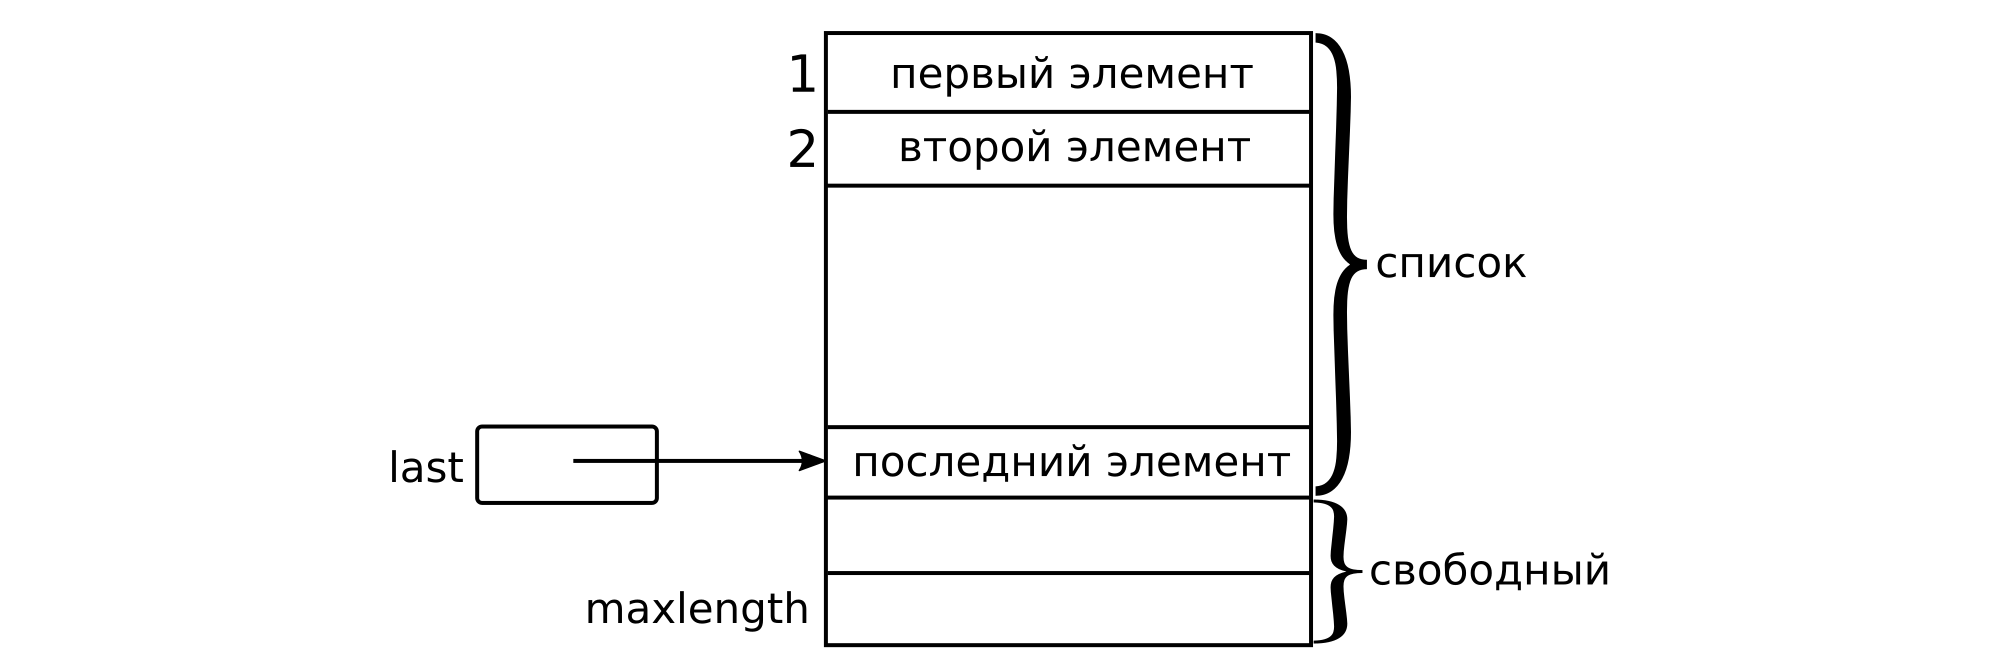
\includegraphics[width=\textwidth]{pictures/48}
\caption{\textit{Представление списка с помощью массива (пояснения в тексте)}}
\end{figure}

При использовании массива мы определяем тип LIST как запись, имеющую два
поля. Первое поле $elements$ (элементы) — это элементы массива, чей размер считается
достаточным для хранения списков любой длины, встречающихся в данной реализации
или программе. Второе поле целочисленного типа $last$ (последний) указывает
на позицию последнего элемента списка в массиве. Как видно из рис. 2.1, $i$-й элемент
списка, если $1 < i < last$, находится $i$-й ячейке массива. Позиции элементов в
списке представимы в виде целых чисел, таким образом, $t$-я позиция — это просто
целое число $i$. Функция END($L$) возвращает значение $last + 1$. Приведем необходимые
объявления (константа $maxlength$ определяет максимальный размер массива):

\begin{lstlisting}[language=C, numbers=none]
    const int;
    maxlenght = 100; //| Или другое подходящее число|
    typedef struct LIST {
        |\textbf{elementtype}| elements[maxlenght];
        int last;
    } list;

    int END (|\textbf{list}| L) {
        return L.last;
    }
\end{lstlisting}

В листинге 2.2 показано, как можно реализовать операторы \rindex{Операторы!списков} INSERT, DELETE и LOCATE при представлении списков с помощью массивов. Оператор INSERT перемещает элементы из позиций $ p, p+1,..., last-1 $ в позиции $ p+1, p+2, ..., last $ и помещает новый элемент в позицию $p$. Если в массиве уже нет места для нового элемента, то инициализируется подпрограмма $error$ (ошибка), распечатывающая соответствующее сообщение, затем выполнение программы прекращается. Оператор DELETE удаляет элемент в позиции $p$, перемещая элементы из позиций $ p+1, p+2,..., last $ в позиции $ p, p+1,..., last-1 $. Функция LOCATE последовательно просматривает элементы массива для поиска заданного элемента. Если этот элемент не найден, то возвращается $ last+1 $.

\begin{lstlisting}[language=C,numbers=none,caption={{Реализация операторов списка}}]
    |\textbf{list}| INSERT (|\textbf{elementtype}| x, int p, list L) {
        //| \textsc{INSERT} вставляет элемент $x$ в позицию $p$ в списке $L$ |
        if (L.last >= maxlenght) {
            printf ("|Список полон|");
        }
        else {
            if (p >= L.last || p < 0) {
                 printf ("|Такой позиции не существует|");
            }
            else {
                for (int i=L.last-1; i > p; i--) {
                    L.elements[i+1] = L.elements[i];
                }
                L.last++;
                L.elements[p] = x;
            }
        }
    return L;
    }

    |\textbf{list}| DELETE (int p, |\textbf{list}| L) {
        //|\textsc{DELETE} удаляет элемент в позиции $p$ списка $L$|
        if (p >= L.last || p < 0) {
            printf ("Такой позиции не существует");
        }
        else {
            L.last--;
            for (int j=p; j<L.last; j++) {
                L.elements[j] = L.elements[j+1];
            }
        }
        return L;
    }

    int LOCATE (|\textbf{elementtype}| x, list L) {
        //|\textsc{LOCATE} возвращает позицию элемента $x$ в списке $L$|
        for (int k=0; k<L.last; k++) {
            if (L.elements[k] == x)
                return k;
        }
    return L.last+1; // элемент не найден
    }
\end{lstlisting}

Легко видеть, как можно записать другие операторы списка, используя данную реализацию списков. Например, функция FIRST всегда возвращает 1, функция NEXT возвращает значение, на единицу большее аргумента, а функция PREVIOUS возвращает значение, на единицу меньшее аргумента. Конечно, последние функции должны делать проверку корректности результата. Оператор MAKENULL(L) устанавливает L.last в 0.

Итак, если выполнению процедуры PURGE (листинг 2.1) предшествуют определения типа elementtype и функции same, объявления типов LIST и position и задание функции END (как показано выше), написание процедуры DELETE (листинг  2.2), подходящая реализация простых процедур FIRST, NEXT и RETRIEVE, то процедура PURGE станет вполне работоспособной программой.

Вначале написание всех этих процедур для управления доступом к основополагающим структурам может показаться трудоемким делом. Но если мы все же подвигнем себя на написание программ в терминах операторов  управления абстрактными типами данными, не задерживаясь при этом на частных деталях их реализаций, то сможем изменять программы, изменяя реализацию этих операторов, не выполняя утомительного  поиска тех мест в программах, где необходимо внести изменения в форму или способ доступа к основополагающим структурам данных. Эта гибкость может иметь определяющее значение при разработке больших программных проектов. К сожалению, читатель не сможет в полной мере оценить эту сторону использования АТД из-за небольших (по размеру) примеров, иллюстрирующих эту книгу.

\subsection*{Реализация списков с помощью указателей}\rindex{Списки!реализация посредством указателей}
\addcontentsline{toc}{subsection}{ Реализация списков с помощью указателей}

В этом разделе для реализации однонаправленных списков \rindex{Списки!однонаправленные} используются указатели, связывающие последовательные элементы списка. Эта реализация освобождает нас от  использования непрерывной области памяти для хранения списка и, следовательно, от необходимости перемещения элементов списка при вставке или удалении элементов. Однако ценой за это удобство становится дополнительная память для хранения указателей.

В этой реализации список состоит из ячеек, каждая из которых содержит элемент списка и указатель на следующую ячейку списка. Если список состоит из элементов $a_1, a_2, ... , a_n$, то для $i=1, 2, ..., n-1$ ячейка, содержащая элемент $a_t$ имеет также указатель на ячейку, содержащую элемент $a_i+1$. Ячейка, содержащая элемент $a_n$, имеет указатель \textbf{nil}\rindex{Указатель!nil} (нуль). Имеется также ячейка $header$ (заголовок), которая указывает на ячейку, содержащую $a_1$. Ячейка $header$ не содержит элементов списка\footnote{Объявление ячейки заголовка "полноценной"\ ячейкой (хотя и не содержащей элементов списка) упрощает реализацию операторов списка. Можете использовать указатели на заголовки, если хотите каким-либо специальным способом реализовать оператор вставки и удаления в самом начале списка.}. В случае пустого списка заголовок имеет указатель nil, не указывающий ни на какую ячейку. На рис. 2.2 показан связанный список описанного вида.

\begin{figure}[ht]
\centering
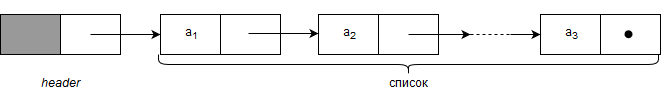
\includegraphics[scale=0.65]{pic51.png}
\caption{\textit{Связанный список}}
\end{figure}

Для однонаправленных списков удобно использовать определение позиций элементов, отличное от того определения позиций, которое применялось в реализации списков с помощью массивов. Здесь для $i= 2, 3, ..., n$ позиция $i$ определяется как указатель на ячейку, содержащую указатель на элемент $a_i$. Позиция 1 — это указатель в ячейке заголовка, а позиция END($L$) — указатель в последней ячейке списка $L$.

Бывает, что тип списка совпадает с типом позиций, т.е. является указателем на ячейку, реже на заголовок. Формально определить структуру связанного списка можно следующим образом:

\begin{lstlisting}[language=C, numbers=none]
    typedef struct LIST {
        |\textbf{elementtype}| element;
        struct LIST *next;
    } |\textbf{list}|;
    |\textbf{list}| L;
    |\textbf{list}| position;
\end{lstlisting}

В листинге 2.3 показан код функции END($L$). Результат функции получаем путем перемещения указателя $q$ от начала списка к его концу, пока не будет достигнут конец списка, который определяется тем, что $q$ становится указателем на ячейку с указателем \textbf{nill}. Отметим, что эта реализация функции END неэффективна, так как требует просмотра всего списка при каждом вычислении этой функции. Если необходимо частое использование данной функции, как в программе PURGE (листинг 2.1), то можно сделать на выбор следующее.

\begin{enumerate}
\item Применить представление списков, которое не использует указатели на ячейки.
\item Исключить использование функции END(L) там, где это возможно, заменив ее другими операторами. Например, условие р!=END(L) в строке (2) листинга 2.1 можно заменить условием p->next!=NULL, но в этом случае программа становится зависимой от реализации списка.
\end{enumerate}

\begin{lstlisting}[language=C,caption={{Функция END}},numbers=none]
    |\textbf{list}| END (|\textbf{list}| L) {
        //|END возвращает указатель на последнюю ячейку-списка $L$|
        |\textbf{list}| q;
        q = L;
        while (q->next != NULL) 
            q = q->next;
        return q;
    }
\end{lstlisting}

Листинг 2.4 содержит процедуры для операторов INSERT, DELETE, LOCATE и MAKENULL, которые используются в реализации списков с помощью указателей. Другие необходимые операторы можно реализовать как одношаговые процедуры, за исключением PREVIOUS, где требуется просмотр списка с начала. Мы оставляем написание этих процедур читателю в качестве упражнений. Отметим, что многие команды не требуют параметра L, списка, поэтому он опущен.

\begin{lstlisting}[language=C,caption={{Реализация некоторых операторов при представлении списков с помощью указателей}}, numbers=none]
    |\textbf{list}|* INSERT (|\textbf{elementtype}| x, |\textbf{list}|* p) {
        |\textbf{list}|* temp; 
        temp=p->next;
        p->next = (|\textbf{list}|*)malloc(sizeof(|\textbf{list}|));
        p->next->element = x;
        p->next->next = temp;
        return p;
    }

    |\textbf{list}|* DELETE (|\textbf{list}|* p) {
        p->next=p->next->next;
        return p;
    }

    |\textbf{list}|* LOCATE (|\textbf{elementtype}| x, |\textbf{list}| L) {
        |\textbf{list}|* p;
        p = L;
        while (p->next != NULL) {
            if (p->next->element == x)
                return p;
            else
                p = p->next;
        }
        return p; //| элемент не найден|
    }

    |\textbf{list}|* MAKENULL (|\textbf{list}|* L) {
        L = (|\textbf{list}|*)malloc(sizeof(|\textbf{list}|));
        L->next = NULL;
        return L;
    }
\end{lstlisting}

Механизм управления указателями в процедуре INSERT (листинг 2.4) показан на рис. 2.3. Рис. 2.3(а) показывает ситуацию перед выполнением  процедуры INSERT. Мы хотим вставить новый элемент перед элементом $b$, поэтому задаем $p$ как указатель на ячейку, содержащую элемент $b$. В строке (4) листинга создается новая ячейка, а в поле $next$ ячейки, содержащей элемент $a$, ставится указатель на новую ячейку. В строке (5) поле $element$ вновь созданной ячейки принимает значения $x$, а в строке (6) поле $next$ этой ячейки принимает значение переменной $temp$, которая хранит указатель на ячейку, содержащую элемент $b$. На рис. 2.3(б) представлен результат выполнения процедуры INSERT, где пунктирными линиями показаны новые указатели и номерами (совпадающими с номерами строк в листинге 2.4) помечены этапы из создания. 

Процедура DELETE более простая. На рис. 2.4 показана схема манипулирования указателем в этой процедуре. Старые указатели показаны сплошными линиями, а новый — пунктирной.
\begin{figure}[ht]
\centering
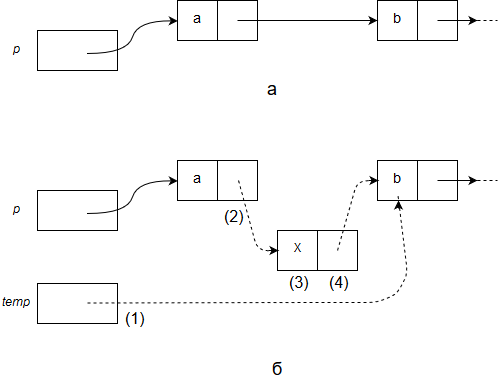
\includegraphics[scale=0.7]{pic53(1).png}
\caption{\textit{Диаграммы, иллюстрирующие работу процедуры INSERT}}
\end{figure}

\begin{figure}[ht]
\centering
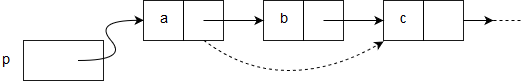
\includegraphics[scale=0.8]{pic53(2).png}
\caption{\textit{Диаграмма, иллюстрирующие работу процедуры DELETE}}
\end{figure}

Еще раз подчеркнем, что позиции в реализации однонаправленных списков ведут себя не так, как позиции в реализации списков посредством массивов. Предположим, что есть список из трех элементов $a$, $b$ и $c$ и переменная $p$ (позиция) типа $list$, чье текущее значение равно позиции 3, т.е. это указатель, находящийся в ячейке, содержащей элемент $b$, и указывающий на ячейку, содержащую элемент $c$. Если теперь мы выполним команду вставки нового элемента $x$ в позицию 2, так что список примет вид $a$, $x$, $b$, $c$, элемент $b$ переместится в позицию 3. Если бы мы использовали реализацию списка с помощью массива, то элементы $b$ и $c$ должны были переместиться к концу массива, так что элемент $b$ в самом деле должен оказаться на третьей позиции. Однако при использовании реализаций списков с помощью указателей значение переменной $p$ (т.е. указатель в ячейке, содержащей элемент $b$) вследствие вставки нового элемента не изменится, продолжая указывать на ячейку, содержащую элемент $c$. Значение этой переменной надо изменить, если мы хотим использовать ее как указатель именно на третью позицию, т.е. как указатель на ячейку, содержащую элемент $b$\footnote[1]{Конечно, можно привести многочисленные примеры ситуаций, когда нужно, чтобы переменная $p$ продолжала указывать на позицию элемента $c$.}.

\subsection*{Сравнение реализаций}\rindex{Списки!сравнение реализаций}
\addcontentsline{toc}{subsection}{ Сравнение реализаций}

Разумеется, нас не может не интересовать вопрос о том, в каких ситуациях лучше использовать реализацию списков с помощью указателей, а когда — с помощью массивов. Зачастую ответ на этот вопрос зависит от того, какие операторы должны выполняться над списками и как часто они будут использоваться. Иногда аргументом в пользу одной или другой реализации может служить максимальный размер обрабатываемых списков. Приведем несколько принципиальных соображений по этому поводу.

\begin{enumerate}
\item Реализация списков с помощью массивов требует указания максимального размера списка до начала выполнения программ. Если мы не можем заранее ограничить сверху длину обрабатываемых списков, то, очевидно, более рациональным выбором будет реализация списков с помощью указателей.
\item  Выполнение некоторых операторов в одной реализации требует больших вычислительных затрат, чем в другой. Например, процедуры INSERT и DELETE выполняются за постоянное число шагов в случае связанных списков любого размера, но требуют времени, пропорционального числу элементов, следующих за вставляемым (или удаляемым) элементом, при использовании массивов. И наоборот, время выполнения функций PREVIOUS и END постоянно при реализации списков посредством массивов, но это же время пропорционально длине списка в случае реализации, построенной с помощью указателей.
\item Если необходимо вставлять или удалять элементы, положение которых указано с помощью некой переменной $position$ типа $list$, и значение этой переменной будет использовано позднее, то не целесообразно использовать реализацию с помощью указателей, поскольку эта переменная не "отслеживает"\ вставку и удаление элементов, как показано выше. Вообще использование указателей требует особого внимания и тщательности в работе.
\item  Реализация списков с помощью массивов расточительна в отношении компьютерной памяти, поскольку резервируется объем памяти, достаточный для максимально возможного размера списка независимо от его реального размера в конкретный момент времени. Реализация с помощью указателей использует столько памяти, сколько необходимо для хранения текущего списка, но требует дополнительную память для указателя каждой ячейки. Таким образом, в разных ситуациях по критерию используемой памяти могут быть выгодны разные реализации.
\end{enumerate}

\subsection*{Реализация списков на основе курсоров}
\addcontentsline{toc}{subsection}{ Реализация списков на основе курсоров}

Некоторые языки программирования, например Fortran\rindex{Fortran} и Algol,\rindex{Algol} не имеют указателей. Если мы работаем с такими языками, то можно смоделировать указатели с помощью курсоров, т.е. целых чисел, которые указывают на позиции элементов в массивах. Для всех списков элементов, имеющих тип elementtype, создадим один массив \textit{SPACE} (область данных), состоящий из записей. Каждая запись будет состоять из поля $element$ для элементов списка и поля $next$ для целых чисел, используемых в качестве курсора. Чтобы создать описанное представление, определим

\begin{lstlisting}[language=C, numbers=none]
    typedef struct {
        |\textbf{elementtype}| element;
        int next;
    } |\textbf{node}|;
    |\textbf{node}| SPACE[maxlength];
\end{lstlisting}

Для списка $L$ объявим целочисленную переменную (например, $Lhead$) в качестве заголовка списка $L$. Можно трактовать $Lhead$ как курсор ячейки заголовка массива $SPACE$ с пустым значением поля $element$. Операторы списка можно реализовать точно так же, как описано выше в случае использования указателей. 

Здесь мы рассмотрим другую реализацию, позволяющую использовать ячейки заголовков для специальных случаев вставки и удаления элементов в позиции 1. (Эту же технику можно использовать и в однонаправленных списках.) Для списка $L$ значение $SPACE[Lhead].element$ равно первому элементу списка, значение $SPACE[Lhead].next$ является индексом ячейки массива, содержащей второй элемент списка, и т.д. Нулевое значение $Lhead$ или нуль в поле $next$ указывает на "указатель nil", это означает, что последующих элементов нет.

Список будет иметь целочисленный тип, поскольку заголовок, представляющий список в целом, является целочисленной переменной. Позиции также имеют тип целых чисел. Мы изменим соглашение о том, что позиция $i$ в списке $L$ является индексом ячейки, содержащей $(i-1)$-й элемент списка $L$, поскольку поле $next$ этой ячейки содержит курсор, указывающий на $i$-й элемент списка. При необходимости первую позицию любого списка можно представить посредством O. Поскольку имя списка является обязательным параметром операторов, использующих позиции элементов, с помощью имен можно различать первые позиции различных списков. Позиция END($L$) — это индекс последнего элемента списка $L$.

На рис. 2.5 показаны два списка, $L$ — $a$, $b$, $c$ и $M$ = $d$, $e$, вложенные в один массив $SPACE$ длиной 10. Отметим, что все ячейки массива, незанятые элементами списков, образуют отдельный список, называемый свободным (ниже в листингах он обозначается $available$). Этот список используется как "источник"\ пустых ячеек при вставке элементов в любой список, а также как место хранения перед дальнейшим использованием освободившихся (после удаления элементов) ячеек.

\begin{figure}[ht]
\centering
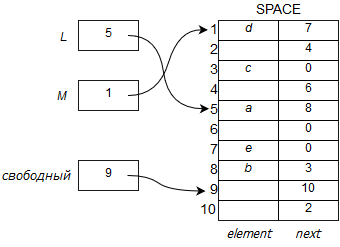
\includegraphics[scale=0.7]{pic(55).png}
\caption{\textit{Реализация связанных списков с использованием курсоров}}
\end{figure}

Для вставки элемента $x$ в список $L$ мы берем первую ячейку из свободного списка и помещаем ее в нужную позицию списка $L$. Далее элемент $x$ помещается в поле $element$ этой ячейки. Для удаления элемента $x$ из списка $L$ мы удаляем ячейку, содержащую элемент $x$, из списка и помещаем ее в начало свободного списка. Эти два действия являются частными случаями следующей операции. Пусть есть ячейка С, на которую указывает курсор $p$, необходимо сделать так, чтобы на ячейку С указывал другой курсор $q$, курсор ячейки С должен указывать на ячейку, на которую ранее указывал курсор $q$, курсор $p$ должен указывать на ячейку, на которую до выполнения этой операции указывал курсор ячейки С. Другими словами, надо переместить ячейку из одного места списка (указываемого курсором $p$) в другое место того же или другого списка, новое место указывается курсором $q$. Например, если необходимо удалить элемент $b$ из списка $L$ (рис. 2.5), то С — это строка 8 в массиве $SPACE$, $p$ равно $SPACE[5].next$, а курсор $q$ указывает на первую ячейку свободного списка. На рис. 2.6 схематически показан процесс перемещения ячейки С из одного списка в другой (курсоры до и после выполнения операции показаны соответственно сплошными и пунктирными линиями). Код функции $move$\rindex{Программа!move} (перемещение), выполняющей описанную операцию, приведен в листинге 2.5. Если в массиве нет ячейки С, то функция возвращает значение $false$ (ложь), при успешном выполнении функции возвращается значение $true$ (истина).

\begin{figure}[ht]
\centering
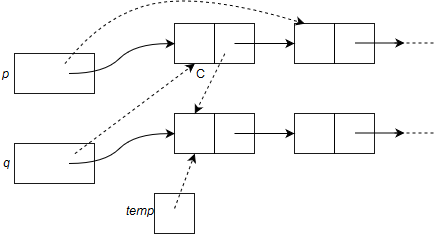
\includegraphics[scale=0.7]{pic56.png}
\caption{\textit{Перемещение ячейки из одного списка в другой}}
\end{figure}

\begin{lstlisting}[language=C,caption={{Функция перемещения ячейки}}, numbers=none]
    int move(int p, int q) {
        int temp;
        if(p == 0) {
            printf("|Ячейка не существует|");
            return 0;
        }
        else {
            temp = q;
            q = p;
            p = SPACE[q].next;
            SPACE[q].next = temp;
            return 1;
        }
    } /* move */
\end{lstlisting}

В листинге 2.6 приведены коды процедур INSERT и DELETE, а также процедуры $initialize$ (инициализация), связывающей ячейки массива $SPACE$ в свободный список. В этих процедурах опущены проверки "нештатных"\ ситуаций, которые могут вызвать ошибки (оставляем написание кода этих проверок читателю в качестве упражнений). Кроме того, в качестве упражнений оставляем читателю реализацию других операторов, выполняемых над списками (их код подобен коду аналогичных процедур при использовании указателей).

\begin{lstlisting}[language=C,caption={{Реализация некоторых операторов списка при использовании курсоров}}, numbers=none]
    void INSERT(|\textbf{elementtype}| x, |\textbf{position}| p, |\textbf{LIST}| L) {
        if(p == 0) {
            if(move(available, L)) /*| вставка $x$ первую позицию |*/
                SPACE[L].element = x;
        }
        else { /*| вставка $x$ в позицию, отличную от первой |*/
            if(move(available, SPACE[p].next))
                SPACE[SPACE[p].next].element = x;
        }
    } /* INSERT */

    void DELETE(|\textbf{position}| p, |\textbf{LIST}| L) {
        if(p == 0)
            move(L, available);
        else
            move(SPACE[p].next, available);
    }/* DELETE */

    void initialize() {
        /*| initialize связывает ячейки \textsc{SPACE} |
                    | в один свободный список |*/
        int i;
        for(i = maxlength-1; i > 1; i--) {
            SPACE[i].next = i+1;
        }
        available = 1;
        SPACE[maxlength].next = 0; /*| помечен конец свобоодного списка |*/
    }/* initialize */
\end{lstlisting}

\subsection*{Дважды связные списки}\rindex{Списки!дважды связные}
\addcontentsline{toc}{subsection}{ Дважды связные списки}

Во многих приложениях возникает необходимость организовать эффективное перемещение по списку как в прямом, так и в обратном направлениях. Или по заданному элементу нужно быстро найти предшествующий ему и последующий элементы. В этих ситуациях можно дать каждой ячейке указатели и на следующую, и на предыдущую ячейки списка, т.е. организовать дважды связный список (рис. 2.7). В главе 12 будут приведены ситуации, когда использование дважды связных списков особенно эффективно.

\begin{figure}[ht]
\centering
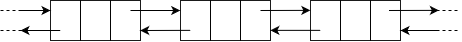
\includegraphics[scale=0.8]{pic57.png}
\caption{\textit{Дважды связный список}}
\end{figure}

Другое важное преимущество дважды связных списков заключается в том, что мы можем использовать указатель ячейки, содержащей $i$-й элемент, для определения $i$-й позиций — вместо использования указателя предшествующей ячейки. Но ценой этой возможности являются дополнительные указатели в каждой ячейке и определенное удлинение некоторых процедур, реализующих основные операторы списка. Если мы используем указатели (а не курсоры), то объявление ячеек, содержащих элементы списка и два указателя, можно выполнить следующим образом ($previous$ — поле, содержащее указатель на предшествующую ячейку):

\begin{lstlisting}[language=C, numbers=none]
    typedef struct LIST {
        |\textbf{elementtype} element;
        struct |\textbf{LIST}| *next;
        struct |\textbf{LIST}| *previous;
    } list;
    |\textbf{list} position;
\end{lstlisting}

Процедура удаления элемента в позиции $p$ дважды связного списка показана в листинге 2.7. На рис. 2.8 приведена схема удаления элемента в предположении, что удаляемая ячейка не является ни первой, ни последней в списке\footnote[1]{В этой связи отметим, что на практике обычно делают так, что ячейка заголовка дважды связного списка "замыкает круг"\ ячеек, т.е. указатель поля $previous$ ячейки заголовка указывает на последнюю ячейку, а указатель поля $next$ — на первую. Поэтому при такой реализации дважды связного списка нет необходимости в выполнении проверки на "нулевой указатель".}. На этой схеме сплошными линиями показаны указатели до удаления, а пунктирными — после удаления элемента. В процедуре удаления сначала с помощью указателя поля $previous$ определяется положение предыдущей ячейки. Затем в поле $next$ этой (предыдущей) ячейки устанавливается указатель, указывающий на ячейку, следующую за позицией $p$. Далее подобным образом определяется следующая за позицией $p$ ячейка и в ее поле $previous$ устанавливается указатель на ячейку, предшествующую позиции $p$. Таким образом, ячейка в позиции $p$ исключается из цепочек указателей и при необходимости может быть использована повторно.

\begin{lstlisting}[language=C,caption={{Удаление элемента из дважды связного списка}}, numbers=none]
    |\textbf{list}|* DELETE (|\textbf{list}|* p) {
        if (p->previous != NULL)
            p->previous->next = p->next;
        if (p->next != NULL)
            p->next->previous = p->previous;
        return p;
    }
\end{lstlisting}

\begin{figure}[ht]
\centering
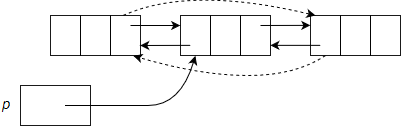
\includegraphics[scale=0.8]{pic58.png}
\caption{\textit{Схема удаления ячейки в дважды связном списке}}
\end{figure}



\section{Стеки}\rindex{Стек}

\textit{Стек} — это специальный тип списка, в котором все вставки и удаления выполняются только на одном конце, называемом \textit{вершиной}\rindex{Стек!вершина} (top). Стеки также иногда называют "магазинами", а в англоязычной литературе для обозначения стеков еще используется аббревиатура LIFO (last-in-first-out — последний вошел — первый вышел). Интуитивными моделями стека могут служить колода карт на столе при игре в покер, книги, сложенные встопку, или стопка тарелок на полке буфета; во всех этих моделях  взять можно только верхний предмет, а добавить новый объект можно, только положив его на верхний. Абстрактные типы данных семейства STACK\rindex{STACK} \rindex{Абстрактный тип данных!STACK} (Стек) обычно используют следующие пять операторов \rindex{Операторы!стеков}.

\begin{enumerate}
\item MAKENULL($S$).Делает стек $S$ пустым.
\item TOP \rindex{Оператор!TOP}($S$). Возвращает элемент из вершины стека $S$. Обычно\rindex{Вершина!стека} вершина стека идентифицируется позицией 1, тогда TOP($S$) можно записать в терминах общих операторов списка как RETRIEVE(FIRST($S$), $S$)
\item POP\rindex{Оператор!POP}($S$). Удаляет элемент из вершины стека (выталкивает из стека), в терминах операторов списка этот оператор можно записать как DELETE(FIRST($S$), $S$). Иногда этот оператор реализуется в виде функции, возвращающей удаляемый элемент.
\item PUSH\rindex{Оператор!PUSH}($x$, $S$). Вставляет элемент $x$ в вершину стека $S$ (заталкивает элемент в стек). Элемент, ранее находившийся в вершине стека, становится элементом, следующим за вершиной, и т.д. В терминах общих операторов списка данный оператор можно записать как INSERT($x$, FIRST($S$), $S$).
\item EMPTY($S$)\rindex{Оператор!EMPTY}. Эта функция возвращает значение $true$ (истина), если стек $S$ пустой, и значение $false$ (ложь) в противном случае.
\end{enumerate}

Пример 2.2. Все текстовые редакторы имеют определенные символы, которые служат в качестве \rindex{Символ!стирающих символов| \textit} (erase character), т.е. таких, которые удаляют (стирают) символы, стоящие перед ними; эти символы "работают"\ как клавиша <Backspace> на клавиатуре компьютера. Например, если символ \# определен стирающим символом, то строка $afrc\#d\#\#e$ в действительности является строкой $ae$. Здесь первый символ \# удаляет букву $c$, второй стирающий символ стирает букву $d$, а третий — букву $b$. 

Текстовые редакторы имеют также символ-убийцу \rindex{Символ!символ-убийцу} (kill character), который удаляет все символы текущей строки, находящиеся перед ним. В этом примере в качестве символа-убийцы определим символ @.

Операции над текстовыми строками часто выполняются с использованием стеков. Текстовый редактор поочередно считывает символы, если считанный символ не является ни символом-убийцей, ни стирающим символом, то он помещается в стек. Если вновь считанный символ — стирающий символ, то удаляется символ в вершине стека. В случае, когда считанный символ является символом-убийцей, редактор очищает весь стек. В листинге 2.7 представлена программа, выполняющая описанные действия.
\rindex{Программа!EDIT}

\begin{lstlisting}[language=C,caption={{Программа, реализующая действия стирающего символа и символа-убийцы}}, numbers=none]
    void EDIT() {
        |\textbf{STACK}|* s;
        char c;
        MAKENULL(s);
        while (c != '\0') {
            c = getch();
            if (c == '#') 
                POP(s);
            else {
                if (c == '@') 
                    MAKEBULL(s);
                else
                    PURSH(c, S);
            }
        }
    }
\end{lstlisting}

В этой программе тип STACK можно объявить как список символов. Процесс вывода содержимого стека в обратном порядке в последней строке программы требует небольшой хитрости. Выталкивание элементов из стека по одному за один раз в принципе позволяет получить последовательность элементов стека в обратном порядке. Некоторые реализации стеков, например с помощью массивов, как описано ниже, позволяют написать простые процедуры для печати содержимого стека, начиная с обратного, конца стека. В общем случае необходимо извлекать элементы стека по одному и вставлять их последовательно в другой стек, затем распечатать элементы из второго стека в прямом порядке. $\Box$

\subsection*{Реализация стеков с помощью массивов}\rindex{Реализация!стеков}\rindex{Стек!реализация посредством массива}
\addcontentsline{toc}{subsection}{ Реализация стеков с помощью массивов}

Каждую реализацию списков можно рассматривать как реализацию стеков, поскольку стеки с их операторами являются частными случаями списков с операторами, выполняемыми над списками. Надо просто представить стек в виде однонаправленного списка, так как в этом случае операторы PUSH и POP будут работать только с ячейкой заголовка и первой ячейкой списка. Фактически заголовок может быть или указателем, или курсором, а не полноценной ячейкой, поскольку стеки не используют такого понятия, как "позиция", и, следовательно, нет необходимости определять позицию 1 таким же образом, как и другие позиции.

Однако реализация списков на основе массивов, описанная в разделе 2.2, не очень подходит для  представления стеков, так как каждое выполнение операторов PUSH и POP в этом случае требует перемещения всех элементов стека и поэтому время их выполнения пропорционально числу элементов в стеке. Можно более рационально приспособить массивы для реализации стеков, если принять во внимание тот факт, что вставка и удаление элементов стека происходит только через вершину стека. Можно зафиксировать "дно"\ стека в самом низу массива (в ячейке с наибольшим индексом) и позволить стеку расти вверх массива (к ячейке с наименьшим индексом). Курсор с именем $top$ (вершина) будет указывать положение текущей позиции первого элемента стека. Схематично такое представление стека показано на рис. 2.9.

\begin{figure}[ht]
\centering
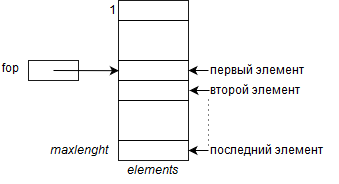
\includegraphics[scale=0.8]{pic60.png}
\caption{\textit{Реализация стека на основе массива}}
\end{figure}

Для такой реализации стеков можно определить абстрактный тип STACK следующим образом:

\begin{lstlisting}[language=C, numbers=none]
    typedef struct |\textbf{STACK}| {
        int top;
        |\textbf{elementtype}| elements[maxlength];
    } |\textbf{STACK}|;
\end{lstlisting}

В этой реализации стек состоит из последовательности элементов $element[top]$, $element[top+1]$,..., $element[maxlength-1]$. Отметим, если $top=maxlength$, то стек пустой. 

Процедуры для реализаций пяти типовых операторов, выполняемых над стеками, представлены в листинге 2.9. Заметим, что значение, возвращаемое функцией ТОР, имеет тип $elementtype$, который должен быть разрешенным типом результата, возвращаемого функцией. Если это не так, данную функцию нужно преобразовать в процедуру или она должна возвращать указатель на элемент типа $elementtype$.

\begin{lstlisting}[language=C,caption={{Реализация операторов над стеками}}, numbers=none]
    void MAKENULL (|\textbf{STACK}|* s) {
        s->top = maxlength;
    }

    int EMPTY (|\textbf{STACK}|* s) {
        if (s->top >= maxlength)
            return 1;
        else
            return 0;
    }

    |\textbf{elementtype}| TOP (|\textbf{STACK}|* s) {
        if (EMPTY(s))
            printf("|Стек пустой|");
        else
            return s->elements[s->top];
    }

    void POP (|\textbf{STACK}|* s) {
        if (EMPTY(s))
            printf("|Стек пустой|");
        else
            s->top = s->top+1;
    }

    void PUSH (|\textbf{elementtype}| x, |\textbf{STACK}|* s) {
        if (s->top == 1)
            printf("|Стек полон|");
        else {
            s->top = s->top - 1;
            s->elements[s->top] = x;
        }
    }
\end{lstlisting}



\section{Очереди}

Другой специальный тип списка — \textit{очередь} (queue), где элементы вставляются с одного  конца, называемого \textit{задним} (rear), а удаляются с другого, \textit{переднего} (front). Очереди также называют "списками типа FIFO"\ (аббревиатура FIFO расшифровывается как
first-in-first-out: первым вошел — первым вышел). Операторы, выполняемые над очередями, аналогичны операторам стеков. Существенное отличие между ними состоит в том, что вставка новых элементов осуществляется в конец списка, а не в начало, как в стеках. Кроме того, различна устоявшаяся терминология для стеков и очередей. Мы будем использовать следующие операторы \rindex{Операторы!очередей} для работы с очередями.

\begin{enumerate}
\item MAKENULL($Q$). Очищает очередь $Q$, делая ее пусой.
\item FRONT\rindex{Оператор!FRONT}($Q$) — функция, возвращающая первый элемент очереди $Q$. Можно реализовать эту функцию с помощью операторов списка как RETRIEVE (FIRST($Q$), $Q$).
\item ENQUEUE($x$, $Q$)\rindex{Оператор!ENQUEUE} вставляет элемент $x$ в конец очереди $Q$. С помощью операторов списка этот оператор можно выполнить следующим образом: INSERT($x$, END($Q$), $Q$).
\item DEQUEUE($Q$)\rindex{Оператор!DEQUEUE} удаляет первый элемент очереди $Q$. Также реализуем с помощью операторов списка как DELETE(FIRST($Q$), $Q$).
\item EMPTY($Q$) возвращает значение $true$ тогда и только тогда, когда $Q$ является пустой очередью.
\end{enumerate}

\subsection*{Реализация очередей с помощью указателей}\rindex{Реализация!операторов очередей}\rindex{Реализация!очередей}
\addcontentsline{toc}{subsection}{ Реализация очередей с помощью указателей}

Как и для стеков, любая реализация списков допустима для представления очередей. Однако, учитывая особенность очереди (вставка новых элементов только с одного, заднего, конца), можно реализовать оператор ENQUEUE более эффективно, чем при обычном представлении списков. Вместо перемещения списка от начала к концу каждый раз при пополнении очереди мы можем хранить указатель (или курсор) на последний элемент очереди. Как и в случае со стеками, можно хранить указатель на начало списка — для очередей этот указатель будет полезен при выполнении команд FRONT и DEQUEUE. В некоторых языках в качестве заголовка можно использовать динамическую переменную и поместить в нее указатель на начало очереди. Это позволяет удобно организовать очищение очереди\footnote[1]{В языке Си, который рассматривается в данной версии учебника, используется тот же прием}. 

Сейчас мы рассмотрим реализацию очередей с использованием указателей языка Си. Читатель может разработать аналогичную реализацию с применением курсоров, но в случае очередей мы имеем возможность более эффективного их (очередей) представления, основанного на массивах, и с непосредственным использованием указателей, чем при попытке моделирования указателей с помощью курсоров. В конце этого раздела мы обсудим также реализацию очередей на основе так называемых "циклических массивов"\rindex{Циклические массивы}. Для начала реализации очередей с помощью массивов необходимо сделать объявление ячеек следующим образом:

\begin{lstlisting}[language=C, numbers=none]
    struct celltype {
        |\textbf{elementtype}| element;
        struct celltype *next;
    };
\end{lstlisting}

Теперь можно определить список, содержащий указатели на начало и конец очереди. Первой ячейкой очереди является ячейка заголовка, в которой поле $element$ игнорируется. Это позволяет, как указывалось выше, упростить представление для любой очереди. Мы определяем АТД QUEUE\rindex{QUEUE} \rindex{Абстрактный тип данных QUEUE} (Очередь)

\begin{lstlisting}[language=C, numbers=none]
    typedef struct QUEUE {
        struct celltype *front, *rear;
    } QUEUE;
\end{lstlisting}

В листинге 2.10 представлены программы для пяти операторов, выполняемых над очередями. В процедуре MAKENULL первый оператор $new(Q.front)$ определяет динамическую переменную (ячейку) типа $celltype$ и назначает ей адрес $Q.front$. Второй оператор этой процедуры задает значение поля $next$ этой ячейки как nil. Третий оператор делает заголовок для первой и последней ячеек очереди.

Процедура DEQUEUE($Q$) удаляет первый элемент из очереди $Q$, "отсоединяя"\ старый заголовок от очереди. Первым элементом списка становится новая динамическая переменная ячейки заголовка.

\begin{lstlisting}[language=C,keepspaces = true, caption={{ Реализация операторов очередей}}]
    void MAKENULL (|\textbf{QUEUE}|* q) {
        q->front = (|\textbf{QUEUE}|*)malloc(sizeof(|\textbf{QUEUE}|));
        q->front->next = NULL;
        q->rear = q->front;
    }

    int EMPTY (|\textbf{QUEUE}|* q) {
        if (q->front == q->rear)
            return 1;
        else
            return 0;
    }

    elementtype FRONT (|\textbf{QUEUE}|* q) {
        if (EMPTY(q))
            printf("|Очередь пуста|");
        else return q->front->next->element;
    }

    void ENQUEUE (|\textbf{elementtype}| x, |\textbf{QUEUE}|* q) {
        q->rear->next = (|\textbf{QUEUE}|*)malloc(sizeof(|\textbf{QUEUE}|));
        q->rear = q->rear->next;
        q->rear->element = x;
        q->rear->next = NULL;
    }

    void DEQUEUE (|\textbf{QUEUE}|* q) {
        if (EMPTY(q))
            printf("|Очередь пуста|");
        else
            q->front = q->front->next;
    }
\end{lstlisting}

На рис. 2.10 показан результат последовательного применения команд \\MAKENULL ($Q$), ENQUEUE ($x$, $Q$), ENQUEUE ($y$, $Q$) и DEQUEUE ($Q$). Отметим, что после исключения из очереди оператором DEQUEUE ($Q$) элемента $x$ он остается в поле $element$ ячейки заголовка, но перестает быть частью очереди.

\begin{figure}[ht]
\centering
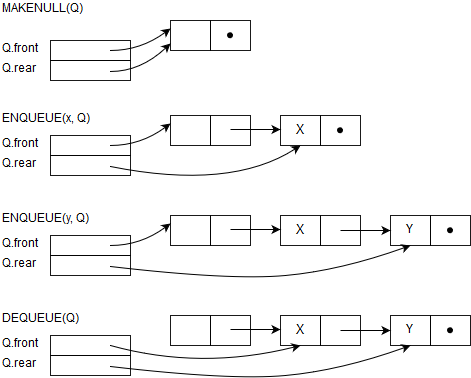
\includegraphics[scale=0.8]{pic64.png}
\caption{\textit{Выполнение последовательности операторов}}
\end{figure}

\subsection*{Реализация очередей с помощью циклических массивов}
\addcontentsline{toc}{subsection}{ Реализация очередей с помощью циклических массивов}

Реализацию списков посредством массивов, которая рассматривалась в разделе 2.2, можно применить для очередей, но в данном случае это не рационально. Действительно, с помощью указателя на последний элемент очереди можно выполнить оператор DEQUEUE за фиксированное число шагов (независимое от длины очереди), но оператор ENQUEUE, который удаляет первый элемент, требует перемещения всех элементов очереди на одну позицию в массиве. Таким образом, ENQUEUE имеет время выполнения $\Omega(n)$, где $n$ — длина очереди.

Чтобы избежать этих вычислительных затрат, воспользуемся другим подходом. Представим массив в виде циклической структуры, где первая ячейка массива следует за последней, как показано на рис. 2.11. Элементы очереди располагаются в "круге"\ ячеек в последовательных позициях\footnote[1]{Отметим, что "последовательность"\ (непрерывность) позиций здесь понимается как "циклическая непрерывность". Например, очередь из четырех элементов может последовательно занимать две последние и две первые ячейки массива.}, конец очереди находится по часовой стрелке на определенном расстоянии от начала. Теперь для вставки нового элемента в очередь достаточно переместить указатель $Q.rear$ (указатель на конец очереди) на одну позицию по часовой стрелке и записать элемент в эту позицию. При удалении элемента из очереди надо просто переместить указатель $Q.front$ (указатель на начало очереди) по часовой стрелке на одну позицию. Отметим, что при таком представлении очереди операторы ENQUEUE и DEQUEUE выполняются за фиксированное время, независимое от длины очереди.

Есть одна сложность представления очередей с помощью циклических массивов и в любых вариациях этого представления (например, когда указатель $Q.rear$ указывает по часовой стрелке на позицию, следующую за последним элементом, а не на сам последний элемент). Проблема заключается в том, что только по формальному признаку взаимного расположения указателей $Q.rear$ и $Q.front$ нельзя сказать, когда очередь пуста, а когда заполнила весь массив. (Конечно, можно ввести специальную переменную, которая будет принимать значение $true$ тогда и только тогда, когда очередь пуста, но если мы не собираемся вводить такую переменную, то необходимо предусмотреть иные средства, предотвращающие переполнение массива).

\begin{figure}[ht]
\centering
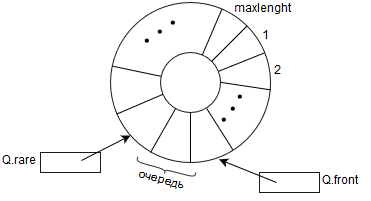
\includegraphics[scale=0.8]{pic65.png}
\caption{\textit{Реализация очереди посредством циклического массива}}
\end{figure}

Чтобы разобраться в этой проблеме, предположим, что очередь состоит из $maxlength$ элементов (рис. 2.11), т.е. полностью заполнила массив. Тогда указатель $Q.rear$ указывает на позицию рядом с Q.front, но находящуюся против часовой стрелки. Что будет, если очередь пуста? Чтобы увидеть представление пустой очереди, сначала положим, что очередь состоит из одного элемента. Тогда указатели $Q.rear$ и $Q.front$ указывают на одну и ту же позицию. Если мы удалим из очереди этот элемент, то указатель $Q.front$ переместится на одну позицию по часовой стрелке, оформляя пустую очередь. Таким образом, в случае пустой очереди указатель $Q.rear$ указывает  на позицию рядом с $Q.front$, находящуюся против часовой стрелки, т.е. точно так же, как и при полном заполнении массива. Отсюда следует вывод, что без введения каких-либо механизмов определения пустых очередей при максимальной длине массива $maxlength$ мы не можем позволить очереди иметь более $maxlength-1$ элементов.

Теперь представим пять команд, выполняемых над очередями, использующими описанную реализацию. Формально очереди здесь определяются следующим образом:

\begin{lstlisting}[language=C, numbers=none]
    typedef struct QUEUE {
        |\textbf{elementtype}| elements[maxlenth];
        int front, rear;
    } QUEUE;
\end{lstlisting}

Соответствующие процедуры показаны в листинге 2.11. Функция $addone(i)$ добавляет единицу к позиции $i$ в "циклическом"\ смысле.

\begin{lstlisting}[language=C,caption={{Реализация очередей с помощью циклических массивов}},numbers=none]
    int addone (int i) {
        return i\%(maxlength-1) + 1;
    }

    void MAKENULL (|\textbf{QUEUE}|* q) {
        q->front = 0;
        q->rear = maxlength-1;
    }

    int EMPTY (|\textbf{QUEUE}|* q) {
        if (addone(q->rear) == q->front))
            return 1;
        else
            return 0;
    }

    |\textbf{elementtype}| FRONT (|\textbf{QUEUE}|* q) {
        if (EMPTY(q))
            printf("|Очередь пустая|");
        else 
            return q->elements[q->front];
    }

    void ENQUEUE (|\textbf{elementtype}| x, |\textbf{QUEUE}|* q) {
        if (addone(q->rear) == q->front)
            printf("|Очередь полная|");
        else {
            q->rear = addone(q->rear);
            q->elements[q->rear] = x;
        }        
    }

    void DEQUEUE (|\textbf{QUEUE}|* q) {
        if (EMPTY(q))
            printf("|Очередь пустая|");
        else
            q->front = addone(q->front);
        }
\end{lstlisting}



\section{Отображения}

\textit{Отображение} — это функция, определенная на множестве элементов (области определения) одного типа (будем обозначать его $domaintype$ — тип области определения функции) и принимающая значения из множества элементов (области значений) другого типа, этот тип обозначим $rangetype$ — тип области значений (конечно, типы $domaintype$ и $rangetype$ могут совпадать). Тот факт, что отображение $M$ ставит в соответствие элемент $d$ типа $domaintype$ из области определения элементу $r$ типа $rangetype$ из области значений, будем записывать как $M(d)=r$.

Некоторые отображения, подобные
$square(i)=i^2$, легко реализовать с помощью функций и арифметических выражений языка C. Но для многих отображений нет очевидных способов реализации, кроме хранения для каждого $d$ значения $M(d)$. Например, для реализации функции, ставящей в соответствие работникам их недельную зарплату, требуется хранить текущий заработок каждого работника. В конце этого раздела мы опишем методы реализации таких функций.

Рассмотрим операторы \rindex{Операторы!отображений}, которые можно выполнить над отображением $M$. Например, по заданному элементу $d$ типа  $domaintype$ мы хотим получить $M(d)$ или узнать, определено ли $M(d)$ (т.е. узнать, принадлежит ли элемент $d$ области определения $M$). Или  хотим добавить новые элементы в текущую область определения $M$ и поставить им в соответствие элементы из области значений. Очевидна также необходимость иметь оператор, который изменял бы значение $M(d)$. Кроме того, нужно средство "обнуления"\ отображения, переводящее любое отображение в \textit{пустое отображение}, т.е. такое, у которого область определения пуста. Наши пожелания можно обобщить в следующие три команды.

\begin{enumerate}
\item MAKENULL($M$). Делает отображение $M$ пустым.
\item ASSIGN($M$, $d$, $r$)\rindex{Оператор!ASSIGN}. Делает $M(d)$ равным $r$ независимо от того, как $M(d)$ было определено ранее.
\item COMPUTE($M$, $d$, $r$).\rindex{Оператор!COMPUTE} Возвращает значение $true$ и присваивает переменной $r$ значение $M(d)$, если последнее определено, и возвращает $false$ в противном случае.
\end{enumerate}

\subsection*{Реализация отображений посредством массивов}
\addcontentsline{toc}{subsection}{ Реализация отображений посредством массивов}

Во многих случаях тип элементов области определения отображения является простым типом, который можно использовать как тип индексов массивов. В языке Си типы индексов включают все конечные интервалы целых чисел, например $1..100$ или $17..23$, строковый тип, диапазоны символов, подобные $'A'...'Z'$, и нечисловые типы, например \textit{север, восток, юг, запад}. В частности, в программах кодирования можно применить отображение $crypt$ (шифратор) с множеством $'A'...'Z'$ и в качестве области определения, и в качестве области значений, так что \textit{сrурt(текст)} будет кодом текста \textit{текст}.

Такие отображения просто реализовать с помощью массивов, предполагая, что некоторые значения типа $rangetype$ могут иметь статус "неопределен". Например, для отображения $crypt$, описанного выше, область значений можно определить иначе, чем $'A'...'Z'$ и использовать символ '?' для обозначения "неопределен". Предположим, что элементы области определения и области значений имеют соответственно типы $domaintype$ и $rangetype$ и что тип $domaintype$ является базовым типом языка C. Тогда тип MAPPING (Отображение) можно объявить следующим образом:

\begin{lstlisting}[language=C, numbers=none]
    typedef struct MAPPING {
        |\textbf{domaintype}| dom;
        |\textbf{rangetype}| M[dom];
    } MAPPING;
\end{lstlisting}

Предполагая, что "неопределен" — это константа типа $rangetype$ и что константы $firstvalue$ и $lastvalue$ равны первому и последнему элементу области определения\footnote[1]{Например, $firstvalue$ = $'A'$ и $lastvalue$ = $'Z'$, если область определения совпадает с множеством $'A'...'Z'$. В листинге 2.12 $domaintype$ принимается за $int$.}, можно реализовать три перечисленных выше оператора, выполняемых над отображениями d листинге 2.12.
\rindex{Словари!реализация посредством массива}
\begin{lstlisting}[language=C, keepspaces = true, caption={{Реализация операторов отображений посредством массива}},numbers=none]
    void MAKENULL (|\textbf{MAPPING}|* M) {
        for (domaintype i=firstvalue; i<=lastvalue; i++) {
            M[i] =| неопределен|;
        } 
    }

    void ASSIGN (|\textbf{MAPPING}|* M, |\textbf{domaintype}| d, |\textbf{rangetype}| r) {
        M[d] = r;
    }

    int COMPUTE (|\textbf{MAPPING}|* M, |\textbf{domaintype}| d, |\textbf{rangetype}| r) {
        if (M[d] ==| неопределен|)
            return 0;
        else {
            r = M[d];
        return 1;
        }
    }
\end{lstlisting}

\subsection*{Реализация отображений посредством списков}
\addcontentsline{toc}{subsection}{ Реализация отображений посредством списков}

Существует много реализаций отображений с конечной областью определения. Например, во многих ситуациях отличным выбором будут хэш-таблицы, которые мы рассмотрим в главе 4. Другие отображения с конечной областью определения можно представить в виде списка пар $(d_1, r_1), (d_2, r_2),..., (d_k, r_k)$, где
$d_1, d_2,..., d_k$ — все текущие элементы области определения, a $r_1, r_2,..., r_k$ — значения, ассоциированные с $d_i (i = 1, 2,..., k)$. Далее можно использовать любую реализацию списков.

Абстрактный тип данных \rindex{Абстрактный тип данных!MAPPING} MAPPING можно реализовать как список типа \\$elementtype$, если сделано объявление

\begin{lstlisting}[language=C, numbers=none]
    typedef struct elementtype {
        |\textbf{domaintype}| domain;
        |\textbf{rangetype}| range;
    } elementtype;
\end{lstlisting}

и затем объявлен тип MAPPING так, как мы ранее объявляли тип LIST (элементов типа  $elementtype$), и в соответствии с той реализацией списков, которую мы выбрали. В листинге 2.13 приведены листинги трех операторов отображения, записанные через операторы списков типа LIST.
\rindex{Реализация!операторов отображений}
\begin{lstlisting}[language=C,keepspaces = true, caption={{Реализация отображения посредством списков}}]
    void MAKENULL (|\textbf{MAPPING}|* M) {
        //|точно такая же, как и для списков|
    }

    void ASSING (|\textbf{MAPPING}|* M, |\textbf{domaintype}| d, |\textbf{rangetype}| r) {
        |\textbf{elementtype}| x;
        |\textbf{list}| p;
        x->domain = d;
        x->range = r;
        p = FIRST(M);
        while (p != END(M)) {
            if (RETRIEVE(p, M)->domain == d)
                DELETE (p, M);
            else
                p = NEXT (p, M);
        }
        INSERT (x, FIRST(M), M);
    }

    int COMPUTE (|\textbf{MAPPING}|* M, |\textbf{domaintype}| d, |\textbf{rangetype}| r) {
        |\textbf{list}| p;
        p = FIRST(M);
        while (p != END(M)) {
            if (RETRIEVE(p, M)->domain == d) {
                r = RETRIEVE(p, M)->range;
                return 1;
            }   
            p = NEXT(p, M);
        }
        return 0; /*| $d$ не принадлежит области определения |*/
    }
\end{lstlisting}



\section{Стеки и рекурсивные процедуры}\rindex{Рекурсивные процедуры}

Стеки находят важное применение при реализации рекурсивных процедур в языках программирования. \textit{Организация выполнения процедур} \rindex{Организация выполнения процедур} в языках программирования  состоит в задании структур данных, которые используются для хранения значений программных переменных во время выполнения программы. Все языки программирования, допускающие рекурсивные процедуры, используют стеки \textit{активационных записей} для хранения всех значений переменных, принадлежащих каждой активной процедуре. При вызове процедуры $P$ новая активационная запись\rindex{Запись!активационная} для этой процедуры помещается в стек независимо от того, есть ли в стеке другие активационные записи \rindex{Активационные записи} для процедуры $P$. Таким образом, извлекая активационную запись из стека, для последнего вызова процедуры $P$, можно управлять возвратом к точке в программе, из которой $P$ вызывалась (эта точка, называемая \textit{адресом возврата}, помещается в активационную запись процедуры $P$ при вызове этой процедуры).

Рекурсивные вызовы процедур упрощают структуру многих программ. Но в некоторых языках программирования процедурные вызовы более "дорогие"\ (по времени выполнения), чем непосредственное выполнение операторов, поэтому программа может работать быстрее, если из нее исключить рекурсивные процедуры. Здесь мы не выступаем в поддержку обязательного исключения рекурсивных или каких-либо иных процедур, очень часто структурная простота программы важна не менее, чем ее малое время выполнения. На практике бывают ситуации, когда после реализации части программного проекта возникает необходимость исключить рекурсию, и основная цель этого обсуждения заключается только в том, чтобы подвести к вопросу о том, как можно преобразовать рекурсивную процедуру в нерекурсивную с помощью стеков.

\textit{Пример 2.3.} Рассмотрим рекурсивное и нерекурсивное решения упрощенной версии классической \textit{задачи о ранце\rindex{Задача!о ранце}}, где мы имеем \textit{целевое значение} $t$ и конечное множество положительных целых \textit{весов} $w_1, w_2,..., w_n$. Необходимо определить, можно ли из множества весов выбрать такой их набор, чтобы их сумма точно равнялась величине $t$. Например, если $t=10$ и множество весов составляют числа 7, 5, 4, 4 и 1, то можно выбрать второй, третий и пятый веса, поскольку 5 + 4 + 1 = 10.

В листинге 2.14 представлена функция $knapsack$\rindex{Программа!knapsack} (ранец), работающая с массивом весов $weights: array[1..n] of integer$. Функция $knapsack(s,i)$ определяет,   существует ли набор весов из множества весов от $weights[i]$ до $weights[n]$, сумма которых равна $s$, и если есть, то печатает этот набор весов. В частном случае, когда $s=0$, пустое множество весов считается решением. Если $s < 0$ или $i > n$ (выход за заданное множество весов), то считаем, что решение не существует или не найдено (функция $knapsack$ возвращает значение $false$).

Если ни один из перечисленных случаев к текущей ситуации не применим, то снова вызывается $knapsack(s-w_i, i+1)$, чтобы посмотреть, существует ли решение, которое включает вес
$w_i$. Если в этом случае решение существует, то оно является и решением исходной задачи; это решение, включая $w_i$, распечатывается. Если решения нет, то вызывается функция $knapsack(s, i+1)$ для поиска решения без участия веса $w_i$. $\Box$

\begin{lstlisting}[language=C,keepspaces = true, caption={{Рекурсивное решение задачи о ранце}}, numbers=none]
    int knapsack ( int target, int candidate) {
        if (target == 0) 
            return 1;
        else {
            if (terget < 0 || candidate > n) {
                return 0;        
            }
            else { //| ищется решение с и без $candidate$|
                if (knapsack(target - weights[candidate], candidate+1)) {
                    printf ("\%d", &weights[candidate]);
                    return 1;
                }
                else //| возможное решение без $candidate$|
                return knapsack (target, candidate+1);
            }
        }
    }
\end{lstlisting}

\subsection*{Исключение "концевых"\ рекурсий}\rindex{Рекурсивные процедуры!исключение}
\addcontentsline{toc}{subsection}{ Исключение "концевых"\ рекурсий}

Часто можно чисто механически исключить последний вызов процедуры самой себя. Если процедура $P(x)$ на последнем шаге вызывает $P(y)$, то этот вызов можно заменить оператором присваивания $x=y$ и последующим переходом в начало кода процедуры $P$. Здесь $y$ может быть выражением, а $x$ должно принимать значение, т.е. это значение хранится в локальной переменной. Если процедура имеет несколько параметров, то с ними надо поступить точно так же, как описано для $x$ и $y$.

Описанная схема вызывает повторное выполнение процедуры $P$ с новым значением параметра $x$ с точно таким же конечным эффектом, какой был бы при рекурсивном вызове $P(y)$ и возврате из этого вызова. Отметим, что тот факт, что некоторые локальные переменные процедуры $P$ принимают новые значения, не имеет последствий, поскольку процедура уже не должна использовать старых значений этих переменных.

Подобный вариант исключения рекурсивного вызова можно проиллюстрировать на примере листинга 2.14, где последний шаг функции $knapsack$ возвращает результат рекурсивного вызова без параметров. В такой ситуации также можно заменить вызов операторами присваивания значений параметрам и переходом в начало кода функции. В данном случае строку (14) в листинге 2.14 можно заменить следующими операторами:

\begin{lstlisting}[language=C, numbers=none]
    candidate++;
    goto beginning;
\end{lstlisting}

где $beginning$ (начало) — метка на оператор строки (2). Отметим, что параметр $target$ не переприсваивается, так как сохраняет старое значение. Поэтому проверки его значения в строках (2) и (5) фактически не нужны, необходимо только проверить условие, что $candidate>n$ в строке (5).

\subsection*{Полное исключение рекурсий\rindex{Исключение рекурсий!полное}}
\addcontentsline{toc}{subsection}{ Полное исключение рекурсий}

Описанная выше техника исключения рекурсивных вызовов полностью удаляет рекурсии только тогда, когда рекурсивные вызовы находятся в конце процедур и вызов осуществляется в форме, позволяющей его исключить. Существует более общий подход, позволяющий преобразовать любую рекурсивную процедуру (или функцию) в нерекурсивную, но этот подход вводит определяемые пользователем стеки. В общем случае этот стек хранит следующее.

\begin{enumerate}
\item Текущие значения параметров процедуры.
\item Текущие значения всех локальных переменных процедуры.
\item Адрес возврата \rindex{Адрес!возврата}, т.е. адрес места, куда должно перейти управление после завершения процедуры.
\end{enumerate}

В случае функции $knapsack$ положение упрощается. Во-первых, заметим, что при всех вызовах (при этом происходит вставка записи в стек) параметр $candidate$ увеличивается на единицу. Поэтому мы можем хранить значение $candidate$ как глобальную переменную, значение которой увеличивается на единицу при вставке записи в стек и уменьшается на единицу при извлечении записи из стека. 

Во-вторых, следующее упрощение можно сделать, если в стеке хранить модифицированный адрес возврата. Отметим, что адрес возврата для этой функции может находиться или в другой процедуре, вызвавшей $knapsack$, или в строке (5), или в строке (8). Можно представить эти три возможности с помощью "статуса", который может принимать три значения.

\begin{enumerate}
\item $none$ (нет). Показывает, что вызов осуществлен из внешней процедуры.
\item $included$ (включенный). Указывает на вызов из строки (5), которая включает вес $weights[candidate]$ в возможное решение.
\item $excluded$ (исключенный). Указывает на вызов из строки (8), которая исключает вес $weights[candidate]$ из возможного решения.
\end{enumerate}

Если мы сохраним статус как адрес возврата, то сможем рассматривать $target$ как глобальную переменную. При изменении статуса с $none$ на $included$ мы вычитаем вес $weights[candidate]$ из $target$ и прибавляем его обратно при изменении статуса с $included$ на $excluded$. Чтобы показать, что рекурсивно вызываемой $knapsack$ найдено решение, используем глобальную переменную $winflag$ (флаг победы). Получив один раз значение $true$, $winflag$ сохраняет это значение, из стека извлекаются записи, и те веса, которые имеют статус $included$, распечатываются. В описанной ситуации стек можно объявить как список статусов ($statuses$) следующим способом:

\begin{lstlisting}[language=C, keepspaces = true, numbers=none]
    typedef struct statuses {поле, included, excluded};
    typedef struct STACK = {подходящее объявление стека};
\end{lstlisting}

В листинге 2.15 приведена  нерекурсивная процедура $knapsack$, оперирующая с массивом весов $weights$. Хотя эта процедура может выполняться быстрее, чем исходная рекурсивная функция $knapsack$, но видно, что код ее длиннее и она труднее для понимания. Поэтому исключение рекурсий следует применять только тогда, когда скорость выполнения программы является решающим фактором.

\begin{lstlisting}[language=C, keepspaces = true, caption={{Нерекурсивная процедура knapsack}},numbers=none]
    void knapsack(int target){
        int canidate;
        bool winflag;
        STACK S;

        candidate = 1;
        winflag = false;
        MAKENULL(S);
        PUSH(none, S);
        /*| инициализация стека для рассмотрения weights[1] |*/
        do{
            if(winflag){
            /*| извлечение записи из стека|
              | и печать весов, входящих в решение |*/
                if(TOP(S) == included)
                    printf();
                candidate--;
                POP(S);
            }   
            else if(target == 0){
                winflag = true;
                candidate--;
                POP(S);
            }
            else{
            /*| решения пока нет, рассматривается |
                      | статус текущего кандидата |*/
            }
            if(TOP(S) == none){
            /*| первая попытка включить кандидата |*/
                target-=weights[candidate];
                candidate++;
                POP(S); 
                PUSH(included, S); 
                PUSH(none, S);
            }
            else if(TOP(S) == included){
            /*| попытка исключить кандидата |*/
                target+=weights[candidate];
                candidate++;
                POP(S); 
                PUSH(included, S); 
                PUSH(none, S);
            }
            else{
            /*| TOP(S) = excluded; отказ от текущего выбора |*/
                POP(S);
                candidate--;
            }
        }
        while(!EMPTY(S))
    }/* knapsack */
\end{lstlisting}

\subsection*{Упражнения}
\addcontentsline{toc}{subsection}{ Упражнения}

\begin{enumerate}
\item[2.1] Напишите с помощью операторов списка программу печати элементов списка.

\item[2.2] Напишите программы вставки, удаления и поиска элементов отсортированного списка, используя для реализации списка \begin{enumerate}
\item[а)] массив;
\item[б)] указатели;
\item[в)] курсоры.
\end{enumerate} Каково время выполнения каждой из этих программ?

\item[2.3] Напишите программу для слияния \begin{enumerate}
\item[а)] двух отсортированных списков;
\item[б)] и отсортированных списков.
\end{enumerate}

\item[2.4] Напишите программу объединения списков в один список.
\item[2.5] Рассмотрим многочлены вида $p(x)=c_1x ^{e_1} + c_2x^{e_2} + ... +c_nx^{e_n}$, где $e_1 > e_2 > ... > e_n \geq 0$. Такой многочлен можно представить в виде связанного списка, где каждая ячейка имеет три поля: одно — для коэффициента $c_i$, второе — для показателя степени $e_i$ третье — для указателя на следующую ячейку. Для описанного представления многочленов напишите программу их дифференцирования.

\item[2.6] Напишите программу сложения и умножения многочленов, используя их представление, описанное в упражнении 2.5.

\item[*2.7] Пусть ячейки объявлены следующим образом:
\begin{lstlisting}[language=C, numbers=none]
    struct _celltype {
        enum _bit {
            1,
            0
        } bit;
        struct _celltype next;
    } celltype;
\end{lstlisting} 
Двоичное число $b_1b_2...b_n$, где каждое $b_i = 0, 1$ имеет десятичное значение $\sum\limits_{i=1}^nb_i2^{n-1}$. Это число можно представить в виде списка $b_1, b_2,..., b_n$. Данный список, в свою очередь, представим как связанный список ячеек типа $celltype$, определенного выше.  Напишите процедуру $increment(bnumber)$, которая прибавляет 1 к двоичному числу $bnumber$. \textit{Совет}: сделайте процедуру $increment$ рекурсивной.

\item[2.8] Напишите процедуру обмена элементами в позициях $p$ и $NEXT(p)$ для простого связанного списка.

\item[*2.9] Следующая процедура предназначена для удаления всех вхождений элемента $x$ в списке $L$. Найдите причину, по которой эта процедура будет выполняться не всегда, и устраните ее.
\begin{lstlisting}[language=C, numbers=none]
    void delete (|\textbf{elementtype}| x, |\textbf{LIST}|* L) {
        |\textbf{list}| p;
        p = FIRST(L);
        while (p != END(L)) {
            if (RETRIEVE(p, L) == x)
                DELETE(p, L);
            p = NEXT(p, L);
        }
    }
\end{lstlisting}

\item[2.10] Необходимо сохранить список в массиве $A$, чьи ячейки содержат два поля: $data$ — для элементов и поле $position$ — для позиций (целых чисел) элементов. Целочисленная переменная $last$ (последний) используется для указания того, что список содержится в ячейках от А[0] до A[$last-1$] массива $A$. Тип LIST определен следующим образом
\begin{lstlisting}[language=C, numbers=none]
    struct node {
        |\textbf{elementtype}| data;
        int position;
    };
    typedef struct LIST {
        int last;
        struct |\textbf{node}|* elements[maxlength]
    } LIST;
\end{lstlisting}
Напишите процедуру DELETE($p$, $L$) для удаления элемента в позиции $p$. Включите в процедуру все необходимые проверки на "внештатные"\ ситуации.

\item[2.11] Пусть $L$ — это список типа LIST, $p$, $q$ и $r$ — позиции. Определите как функцию от $n$ (длины списка $L$) количество выполнений функций FIRST, END и NEXT в следующей программе
\begin{lstlisting}[language=C, numbers=none]
    p = FIRST(L);
    while (p != END(L)) {
        q = p;
        while (q != END(L)) {
            q = NEXT(q, L);
            r = FIRST(L);
            while (r != q)
                r = NEXT(r, L);
        }
        p = NEXT (p, L);
    }
\end{lstlisting}

\item[2.12] Перепишите код операторов, выполняемых над списками LIST, в предположении, что реализуются однонаправленные списки.

\item[2.13] Добавьте необходимые проверки на ошибки в процедуры листинга 2.6.

\item[2.14] Еще одна реализация списков посредством массивов совпадает с описанной в разделе 2.2 за исключением того, что при удалении элемента он заменяется значением "удален", которое другим способом в списке появиться не может. Перепишите операторы списка для этой реализации. Какие достоинства и недостатки этой реализации списков по сравнению с исходной?

\item[2.15] Предположим, что мы хотим использовать логическую переменную при реализации очереди для указания того, что очередь пуста. Измените объявления и операторы в реализации очередей посредством циклических массивов для использования этой переменной. Что можно ожидать от такой рационализации?

\item[2.16] \textit{Очередь с двусторонним доступом} — это список, в котором добавлять и удалять элементы можно с обоих концов. Разработайте реализации для таких очередей с использованием массивов, указателей и курсоров.

\item[2.17] Определите АТД, поддерживающие операторы ENQUEUE, DEQUEUE (см. раздел 2.4) и ONQUEUE. ONQUEUE($x$) — функция, возвращающая значения $true$ или $false$ в зависимости от того, присутствует или нет элемент $x$ в очереди.

\item[2.18] Как реализовать очередь, если элементами являются символьные строки произвольной длины? Сколько времени необходимо для операции вставки такого элемента в очередь?

\item[2.19] В одной возможной реализации очередей посредством связанных списков не используется ячейка заголовка, а указатель $front$ указывает  непосредственно на первую ячейку. Если очередь пуста, тогда $front$ = $rear$ = nil. Напишите необходимые операторы для этой реализации очередей. Сравните эту реализацию с реализацией, описанной в разделе 2.4, по критериям времени выполнения, требуемого объема памяти и лаконичности (краткости и понятности) кода.

\item[2.20] В одном варианте реализации очередей посредством циклических массивов записываются позиция первого элемента и длина очереди.
\begin{enumerate}
\item[а)] необходимо ли в этой реализации ограничивать длину очереди числом $maxlength-1$?
\item[б)] напишите пять операторов, выполняемых над очередями, для этой реализации;
\item[в)] сравните эту реализацию с реализацией посредством циклических массивов, описанной в разделе 2.4.
\end{enumerate}
\item[2.21] Возможно хранение двух стеков в одном массиве, если один располагается в начале массива и растет к концу массива, а второй располагается в конце массива и растет к началу. Напишите процедуру PUSH($x$, $S$) вставки элемента $x$ в стек $S$, где $S$ — один или другой стек из этих двух стеков. Включите все необходимые проверки в эту процедуру.
\end{enumerate}

Можно хранить $k$ стеков в одном массиве, если используется структура данных, показанная на рис. 2.12 для случая $k = 3$. В этом случае можно организовать вставку и удаление элементов для каждого стека так же, как описано в разделе 2.3. Но если случится, что при вставке элемента в стек $i$ вершина $TOP(i)$ совпадет с "дном"\ предыдущего стека $BOTTOM(i-1)$, то возникает необходимость переместить все стеки так, чтобы между каждой парой смежных стеков был зазор из пустых ячеек массива. В этом случае мы можем сделать все зазоры одинаковыми или пропорциональными длине соседнего с зазором стека (из теории следует: чем больше стек, тем вероятнее в ближайшем будущем его рост, а мы, естественно, хотим отсрочить следующую реорганизацию массива).

\begin{enumerate}[topsep=0pt,itemsep=1ex,partopsep=1ex,parsep=1ex]
\renewcommand{\labelenumii}{\theenumii)}

%%      ЗАМЕНИТЬ НА БУКВЕННУЮ НУМЕРАЦИЮ СПИСКА

\item В предположении, что есть процедура \textit{reorganize} (реорганизация), вызываемая
при возникновении "конфликтов"\ между стеками, напишите код для пяти
операторов стека;

\item Напишите процедуру \textit{reorganize} в предположении, что уже существует процедура
makenewtops (сделать новые вершины), которая вычисляет $neu>top[i]$, —
новую позицию вершины стека $i$ для всех $i, I < i < k$. Совет: отметим, что
стек $i$ может перемещаться как вверх, так и вниз по массиву. Если новая позиция
стека $j$ захватывает старую позицию стека $i$, то стек $i$ надо переместить
раньше стека $j$. Рассматривая стеки в порядке $1, 2, ..., k,$ создадим еще стек
"целей"\ , каждая "цель"\ будет перемещать отдельный конкретный стек. Если
стек $i$ можно безопасно переместить, то перемещение выполняется и повторно
рассматривается стек, чей номер находится в вершине стека целей. Если стек
$i$ нельзя переместить, не затрагивая других стеков, то его номер помещается в
стек целей;

\item Какая подходящая реализация для стека целей? Необходимо ли для этого использовать
список из целых чисел или можно воспользоваться более простой
реализацией?

\item Реализуйте процедуру \textit{makenewtops} так, чтобы пространство перед каждым
стеком было пропорционально его текущей длине;

\item Какие изменения надо сделать в схеме рис. 2.12, чтобы ее можно было применить
для очередей? А для произвольных списков?
\end{enumerate}

\begin{figure}[ht]
\centering
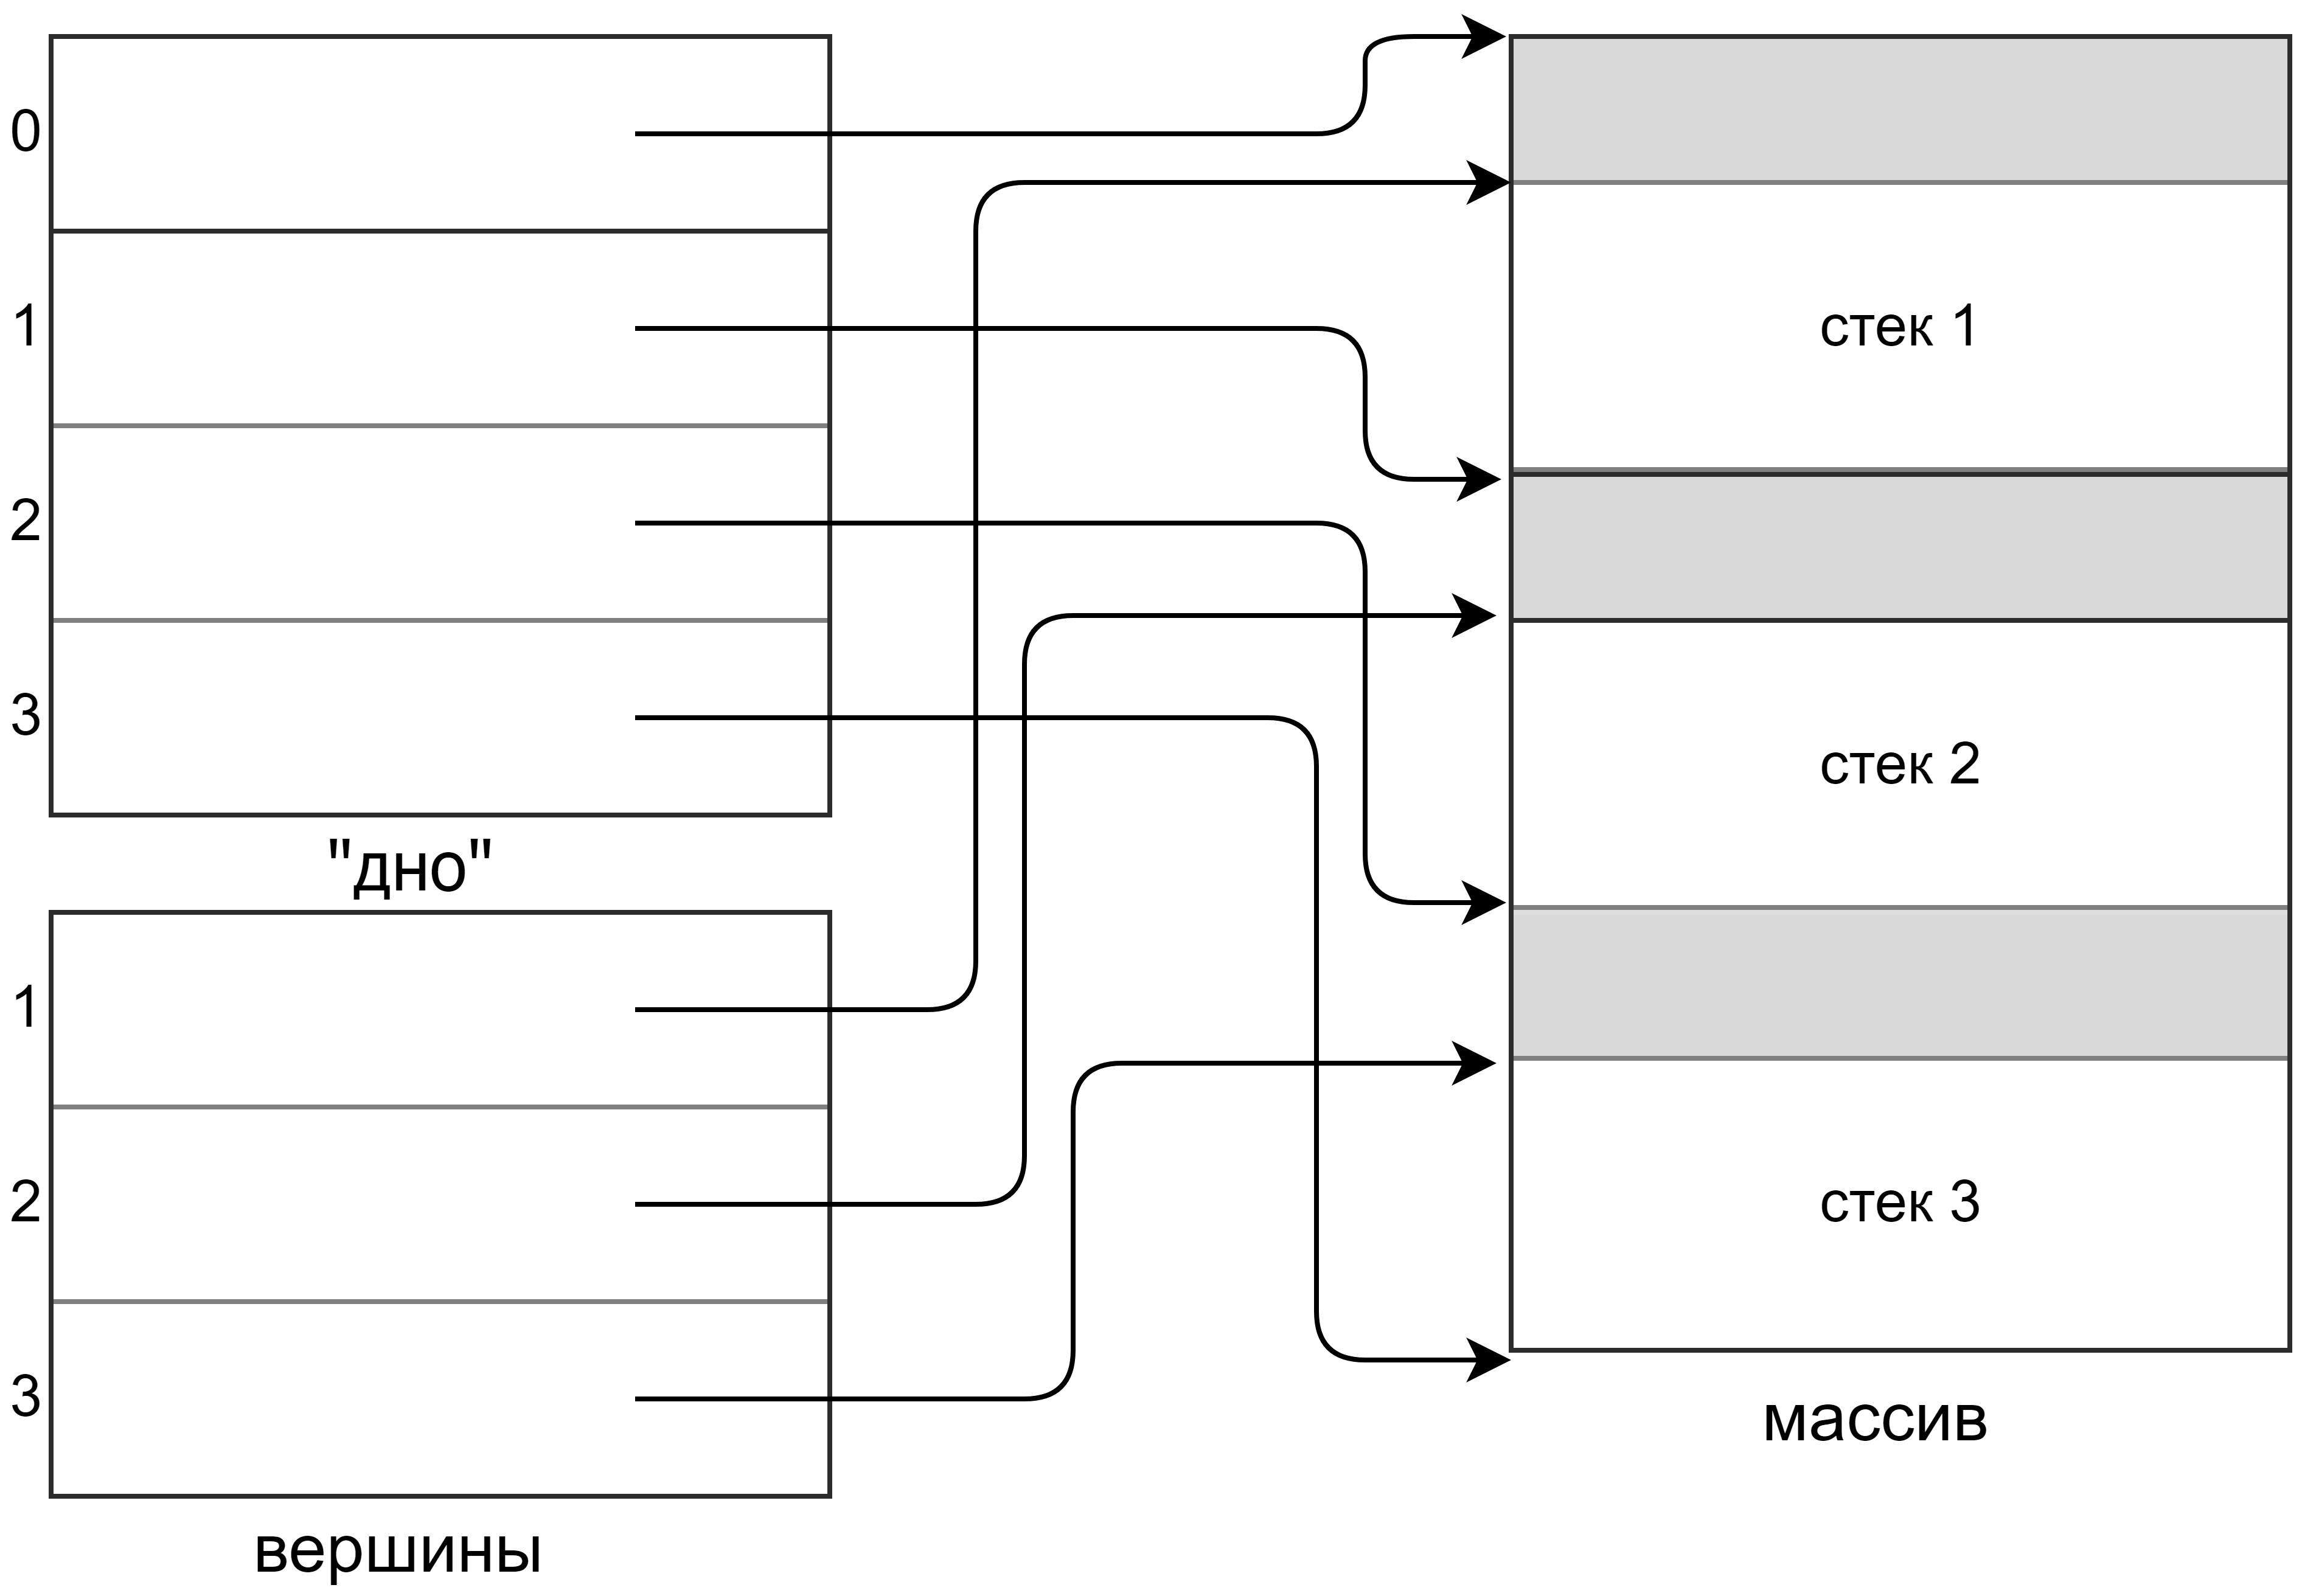
\includegraphics[scale=0.085]{pictures/p73}
\caption{Расположение нескольких стеков в одном массиве}
\end{figure} 

%\item
Измените реализации операторов $POP$ и $ENQUEUE$ из разделов 2.3 и 2.4 так, чтобы они возвращали элементы, удаленные соответственно из стека и очереди. Что необходимо сделать, если элемент имеет тип данных, который функция не может вернуть?
%\item
Используйте стек для исключения рекурсивных вызовов из следующей процедуры:

%%      ЗАМЕНИТЬ НА БУКВЕННУЮ НУМЕРАЦИЮ СПИСКА

\begin{lstlisting}[language=C,keepspaces = true, numbers=none]* 
    int comb(int n, int m){ 
        /*| Вычисление  биномиальных коэффициентов |*/
        if((n == 1) ll (m == 0) ll (m == n))
            return 1;
        else
            return comb(n-1, m) + comb(n-1, m-1);
    }
\end{lstlisting}

%\item
Можно ли исключить последние рекурсивные вызовы из программ примера
2.24? Если можно, то как?


\subsection*{Библиографические примечания}
\addcontentsline{toc}{subsection}{ Библиографические примечания}

Книга [63] содержит дополнительный материал по реализациям списков, стеков и
очередей. Многие языки программирования, например LISP и SNOBOL, поддерживают
списки в удобной форме. См. работы [80], [86], [94] и [117], содержащие исторические
справки и описания таких языков.


\newpage

%		НОМЕР ГЛАВЫ (ГЛОБАЛЬНО)

\chapter{Деревья}
\thispagestyle{empty}

Деревья представляют собой иерархическую структуру некой совокупности элементов.\rindex{Дерево}
Знакомыми вам примерами деревьев могут служить генеалогические и организационные
диаграммы.\rindex{Дерево!2-3\see{Дерево 2-3}} Деревья используются при анализе электрических цепей, при представлении
структур математических формул. Они также естественным путем возникают
во многих областях компьютерных наук. Например, деревья используются для организации
информации в системах управления базами данных и для представления
синтаксических структур в компиляторах программ. В главе 5 описано применение деревьев
для представления данных. В этой книге вы встретитесь со многими примерами
деревьев. В этой главе мы введем основные определения (терминологию) и представим
основные операторы, выполняемые над деревьями. Затем опишем некоторые наиболее
часто используемые структуры данных, представляющих деревья, и покажем, как
наиболее эффективно реализовать операторы деревьев.

\section{Основная терминология}

Дерево\rindex{Дерево!определение} — это совокупность элементов, называемых \textit{узлами}\rindex{Узел дерева} (один из которых определен
как \textit{корень})\rindex{Корень!дерева}, и отношений ("родительских"), образующих иерархическую
структуру узлов. Узлы, так же, как и элементы списков, могут быть элементами любого
типа. Мы часто будем изображать узлы буквами, строками или числами. Формально
\textit{дерево} можно рекуррентно определить следующим образом.

\begin{enumerate}[topsep=0pt,itemsep=1ex,partopsep=1ex,parsep=1ex]
\item Один узел является деревом. Этот же узел также является корнем этого дерева.
\item Пусть $n$ — это узел, а $T_1$, $T_2$, ..., $T_k$  — деревья с корнями $n_1$,  $n_2$, ... ,  $n_k$, соответственно.
Можно построить новое дерево, сделав $n$ родителем\rindex{Узел дерева!родитель} узлов  $n_1$,  $n_2$, ... ,  $n_k$. В этом дереве $n$ будет корнем,
a $T_1$, $T_2$, ..., $T_k$ — поддеревьями\rindex{Поддерево} этого корня. Узлы $n_1$,  $n_2$, ... ,  $n_k$
и называются \textit{сыновьями}\rindex{Узел дерева!сыновья} узла $n$.
\end{enumerate} %%		ОТСУТП ПОСЛЕ СПИСКА

Часто в это определение включают понятие \textit{нулевого дерева},\rindex{Дерево!нулевое} т.е. "дерева" \ без узлов,
такое дерево мы будем обозначать символом $\Lambda$.


\indent \textbf{Пример 3.1.} Рассмотрим оглавление книги, схематически представленное на
рис. 3.1, а. Это оглавление является деревом, которое в другой форме показано на
рис. 3.1, б. Отношение родитель-сын отображается в виде линии. Деревья обычно рисуются
сверху вниз, как на рис. 3.1, б, так, что родители располагаются выше "детей".

\begin{figure}[ht]
\centering
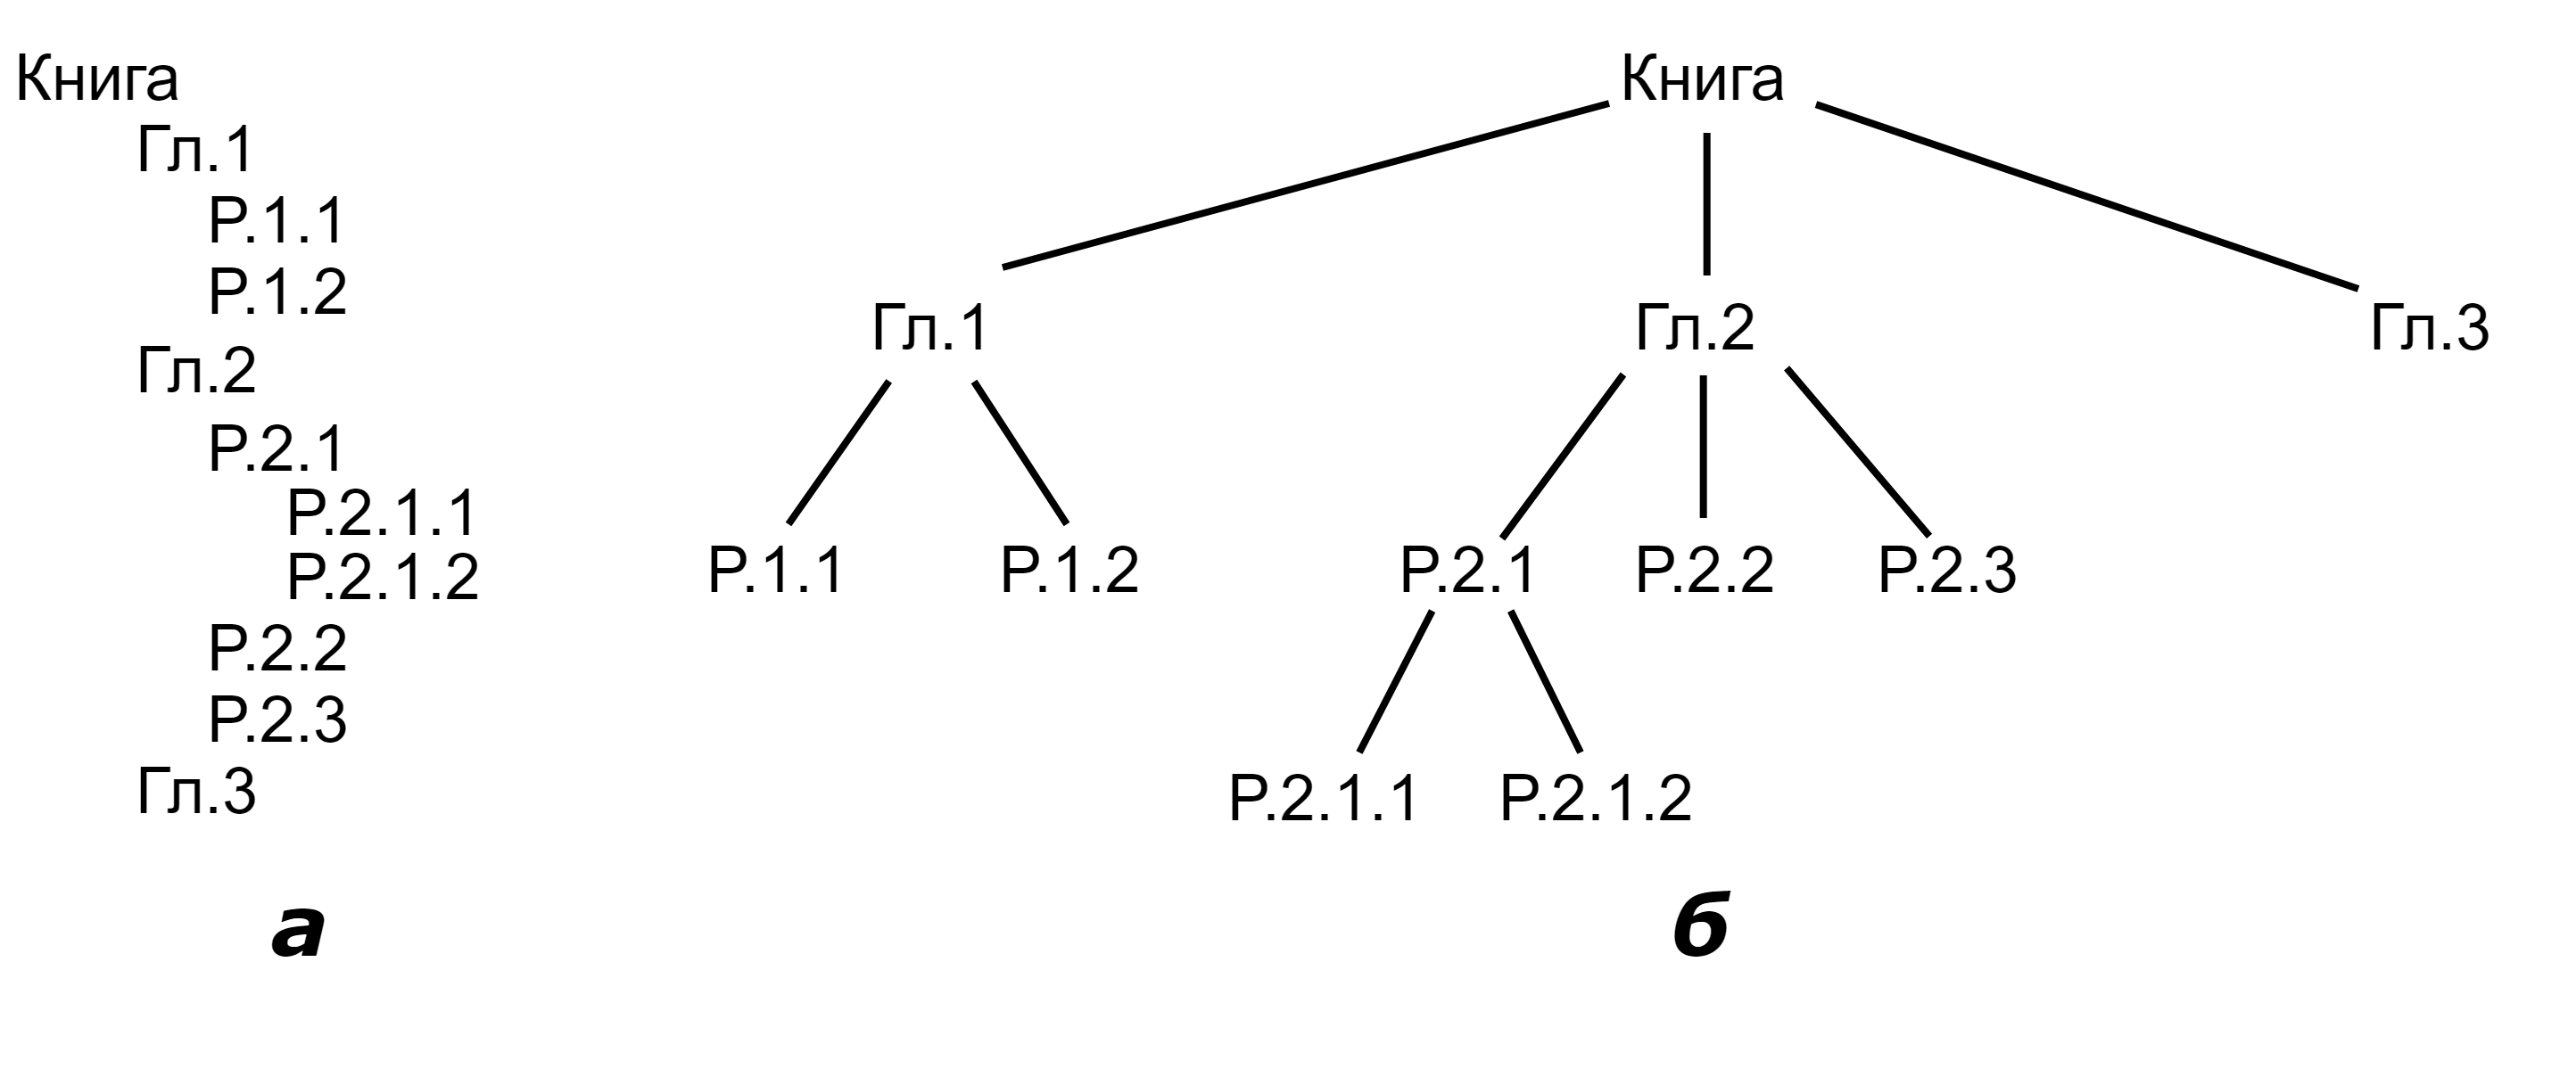
\includegraphics[scale=0.14]{pictures/p75}
\caption{Оглавление книги и его представление в виде дерева}
\end{figure} 

\indentКорнем этого дерева является узел \textit{Книга}, который имеет три поддерева соответственно
с корнями \textit{Гл.1, Гл.2} и \textit{Гл.З}. Эти отношения показаны линиями, идущими из
корня \textit{Книга} к узлам \textit{Гл.1, Гл.2} и \textit{Гл.З}. Узел \textit{Книга} является родителем узлов  \textit{Гл.1, Гл.2} и \textit{Гл.З}, а эти три узла — сыновьями узла \textit{Книга}.

\indentТретье поддерево, с корнем \textit{Гл.З}, состоит из одного узла, остальные два поддерева
имеют нетривиальную структуру. Например, поддерево с корнем \textit{Гл.2} в свою очередь
имеет три поддерева, которые соответствуют разделам книги \textit{Р.2.1, Р.2.2 и Р.2.3}; последние
два поддерева имеют по одному узлу, в то время как первое имеет два поддерева,
соответствующие подразделам книги \textit{Р.2.1.1} и \textit{Р.2.1.2.}. $\square $


\indentПример 3.1 показывает типичные данные, для которых наилучшим представлением
будут деревья. В этом примере родительские отношения устанавливают подчиненность
глав и разделов: родительский узел связан с узлами сыновей (и указывает
на них), как узел Книга подчиняет себе узлы \textit{Гл.1, Гл.2} и \textit{Гл.З}. В этой книге вы
встретите много различных отношений, которые можно представить с помощью родительских
отношений и подчиненности в виде деревьев.
\\ \indent \textit{Путем} \rindex{Дерево!путь} \rindex{Граф!путь} \rindex{Путь!в дереве} из узла $n_1$ в узел $n_k$, называется последовательность узлов $n_1, n_2, ... , n_k$
где для всех $i, 1 \leq i \leq k,$ узел $n_i$
является родителем узла $n_{i+1}$. \textit{Длиной пути} \rindex{Длина пути} называется
число, на единицу меньшее числа узлов, составляющих этот путь. Таким образом,
путем нулевой длины будет путь из любого узла к самому себе. На рис. 3.1 путем
длины 2 будет, например, путь от узла \textit{Гл.2} к узлу \textit{Р.2.1.2}.

\indentЕсли существует путь из узла $a$ в $b$, то в этом случае узел $a$ называется \textit{предком}\rindex{Узел дерева!предок}
узла $b$, а узел $b$ — потомком узла\rindex{Узел дерева!потомок} $a$. Например, на рис. 3.1 предками узла \textit{Р.2.1} будут
следующие узлы: сам узел \textit{Р.2.1} и узлы \textit{Гл.2} и \textit{Книга}, тогда как потомками этого
узла являются опять сам узел \textit{Р.2.1} и узлы \textit{Р.2.1.1} и \textit{Р.2.1.2}. Отметим, что любой узел
одновременно является и предком, и потомком самого себя.

\indentПредок или потомок узла, не являющийся таковым самого себя, называется истинным
предком\rindex{Узел дерева!истинный предок} или истинным потомком\rindex{Узел дерева!истинный потомок} соответственно. В дереве только корень
не имеет истинного предка. Узел, не имеющий истинных потомков, называется листом\rindex{Лист дерева}.
Теперь поддерево какого-либо дерева можно определить как узел (корень поддерева)
вместе со всеми его потомками.

\indentВысотой узла\rindex{Узел дерева!высота} дерева называется длина самого длинного пути из этого узла до
какого-либо листа. На рис.3.1 высота узла \textit{Гл.1} равна 1, узла \textit{Гл.2} — 2, а узла \textit{Гл.З} —
0.\rindex{Высота дерева} \rindex{Дерево!высота}Высота дерева совпадает с высотой корня. \textit{Глубина узла}\rindex{Узел дерева!глубина} определяется как длина
пути (он единственный) от корня до этого узла.

\subsection*{Порядок узлов}\rindex{Дерево!порядок узлов}
\addcontentsline{toc}{subsection}{ Порядок узлов}

\indent Сыновья узла обычно упорядочиваются слева направо. Поэтому два дерева на рис.
3.2 различны, так как порядок сыновей узла $a$ различен. Если порядок сыновей игнорируется,
то такое дерево называется \textit{неупорядоченным},\rindex{Дерево!неупорядоченное} в противном случае дерево
называется \textit{упорядоченным}.\rindex{Дерево!упорядоченное}

\begin{figure}[ht]
\centering
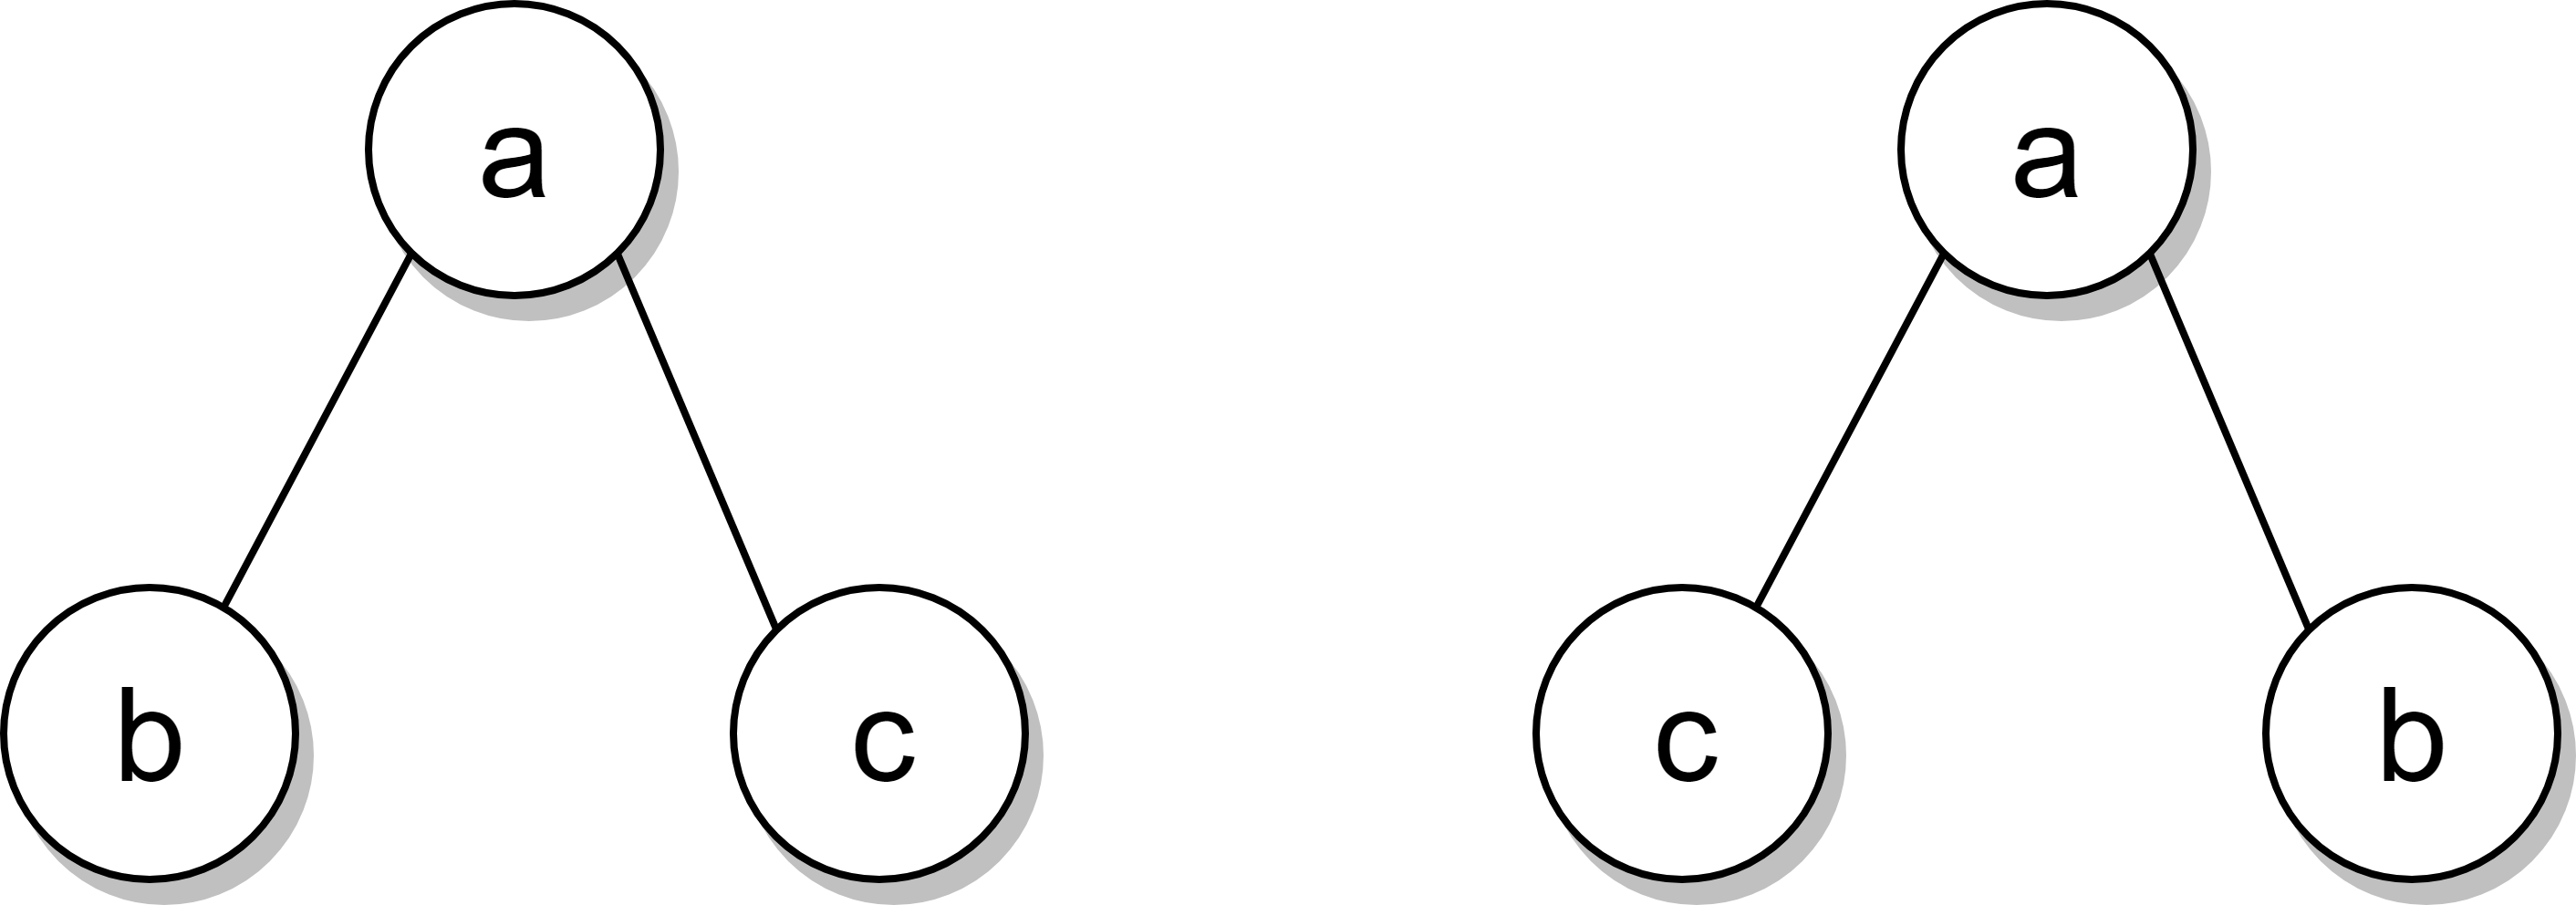
\includegraphics[scale=0.1]{pictures/p76}
\caption{Два различных упорядоченных дерева}
\end{figure} 

Упорядочивание слева направо \textit{сыновей} ("родных детей" одного узла) можно использовать
для сопоставления узлов, которые не связаны отношениями предкипотомки.
Соответствующее правило звучит следующим образом: если узлы $a$ и $b$ являются
сыновьями одного родителя и узел $a$ лежит слева от узла $b$, то все потомки
узла $a$ будут находиться слева от любых потомков узла $b$.
\\ \indent \textbf{Пример 3.2}. Рассмотрим дерево на рис. 3.3. Узел 8 расположен справа от узла 2,
слева от узлов 9, 6, 10, 4 и 7, и не имеет отношений справа-слева относительно предков
1, 3 и 5.

\begin{figure}[ht]
\centering
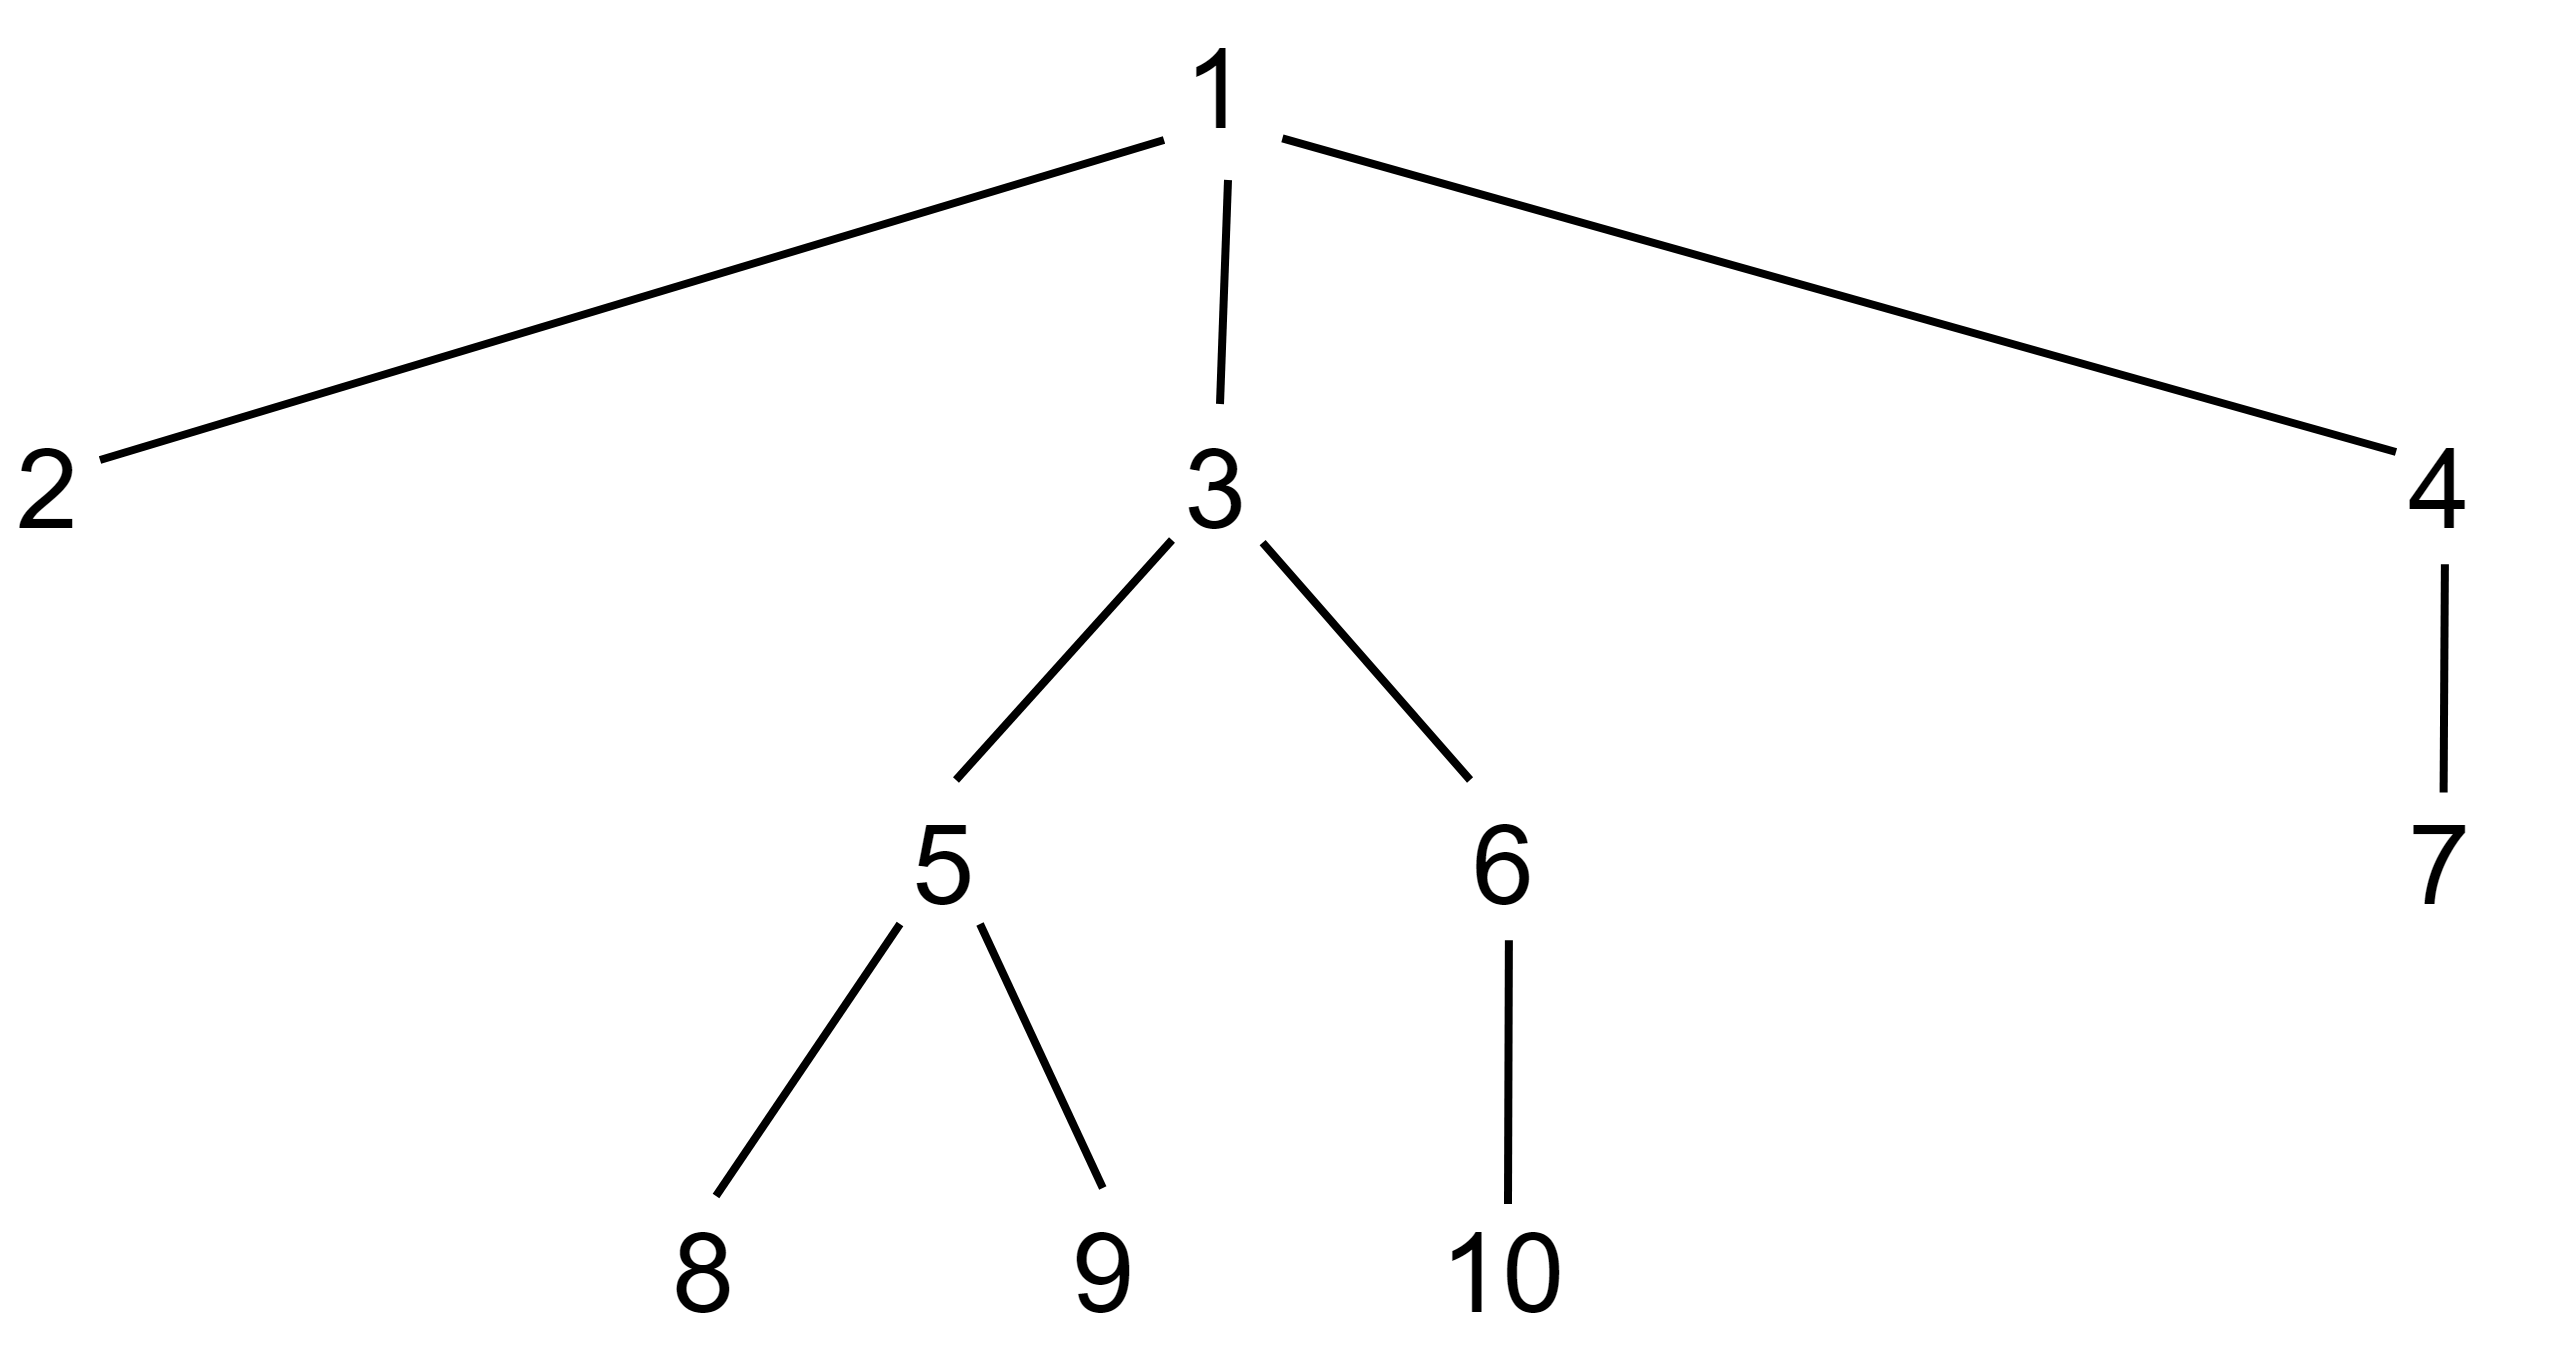
\includegraphics[scale=0.1]{pictures/p77_1}
\caption{Дерево}
\end{figure} 

\indent Существует простое правило, позволяющее определить, какие узлы расположены
слева от данного узла $n$, а какие — справа. Для этого надо прочертить путь от корня
дерева до узла $n$. Тогда все узлы и их потомки, расположенные слева от этого пути,
будут находиться слева от узла $n$, и, аналогично, все узлы и их потомки, расположенные
справа от этого пути, будут находиться справа от узла $n$. $\square$


\subsection*{Прямой, обратный и симметричный обходы дерева}\rindex{Дерево!способы обхода}
\addcontentsline{toc}{subsection}{ Прямой, обратный и симметричный обходы дерева}

\indent Существует несколько способов обхода (прохождения) всех узлов дерева\footnote[1]{Обход узлов дерева равнозначен упорядочиванию по какому-либо правилу этих узлов. Поэтому
в данном разделе мы будем использовать слова "обход узлов"\ и "упорядочивание узлов"\ как синонимы. — \textit{Прим. ред}.}. 
Три наиболее часто используемых способа обхода дерева называются обход в \textit{прямом порядке},
обход в \textit{обратном порядке} и обход во \textit{внутреннем порядке} (последний вид обхода
также часто называют \textit{симметричным обходом}, мы будем использовать оба этих
названия как синонимы). Все три способа обхода рекурсивно можно определить следующим
образом.

\begin{enumerate}[topsep=0pt,itemsep=1ex,partopsep=1ex,parsep=1ex]
\item Если дерево $T$ является нулевым деревом, то в список обхода заносится пустая
запись.
\item  Если дерево $T$ состоит из одного узла, то в список обхода записывается этот узел.
\item Далее, пусть $T$ — дерево с корнем $n$ и поддеревьями $T_1, T_2, ... , T_k$ 
, как показано
на рис. 3.4. Тогда для различных способов обхода имеем следующее.
\end{enumerate}

\begin{figure}[!ht]
\centering
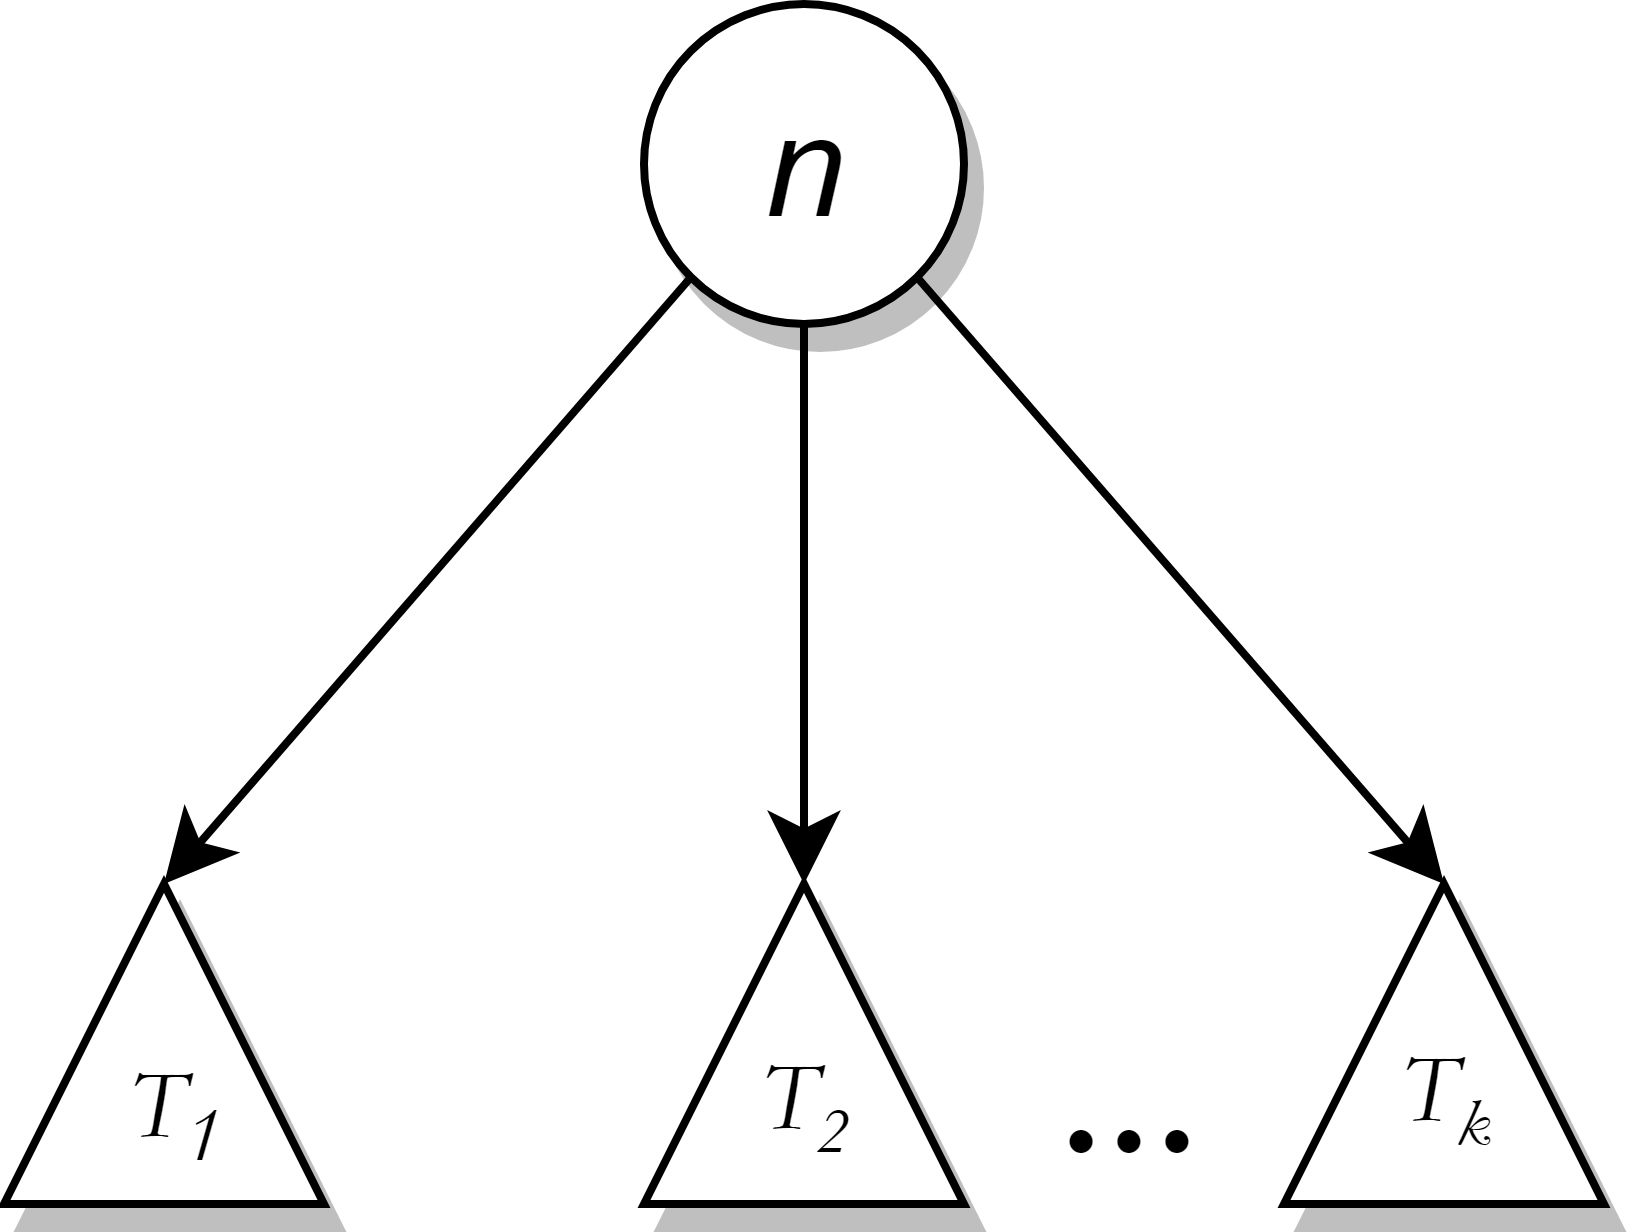
\includegraphics[scale=0.1]{pictures/p77_2}
\caption{Дерево $T$}
\end{figure} 

\newpage

\begin{enumerate}[topsep=0pt,itemsep=1ex,partopsep=1ex,parsep=1ex]
\item При \textit{прохождении в прямом порядке} (т.е. при \textit{прямом упорядочивании}) узлов дерева
$T$ сначала посещается корень $n$, затем узлы поддерева $T_1$, далее все узлы
поддерева $T_2$
, и т.д. Последними посещаются узлы поддерева $T_k$.
\item  При симметричном обходе узлов дерева $T$ сначала посещаются в симметричном
порядке все узлы поддерева $T_1$, далее корень $n$, затем последовательно в симметричном
порядке все узлы поддеревьев $T_2, ... , T_k$
\item Во время \textit{обхода в обратном порядке} сначала посещаются в обратном порядке
все узлы поддерева $T_1$ затем последовательно посещаются все узлы поддеревьев
$T_2, ... , T_k$, также в обратном порядке, последним посещается корень $n$.
\end{enumerate}

%%		ОТСУТП ПОСЛЕ СПИСКА

\indent В листинге 3.1 показан набросок процедуры PREORDER\rindex{Программа!PREORDER} (Прямое упорядочивание),
составляющей список узлов дерева при обходе его в прямом порядке. Чтобы из
этой процедуры сделать процедуру, выполняющую обход дерева в обратном порядке,
надо просто поменять местами строки (1) и (2). Также в листинге 3.1 представлен набросок\rindex{Обход дерева!в прямом порядке}
процедуры INORDER\rindex{Программа!INORDER} (Внутреннее упорядочивание). В этих процедурах производится
соответствующее упорядочивание деревьев путем вызова соответствующих
процедур к корню дерева.\rindex{Обход дерева!в обратном порядке}
\rindex{Обход дерева!в симметричном порядке}
\begin{lstlisting}[caption = {Рекурсивные процедуры обхода деревьев}, captionpos=t, numbers=none] 
    void PREORDER(|\textbf{Node}|* root){
(1)    	|занести в список обхода узел $n$|;
(2)    	for| для каждого сына c узла $n$| 
                    |в порядке слева направо |do{
          PREORDER(c);
        }
    }

    void INORDER(|\textbf{Node}|* root){
        if n -| лист|
            |занести в список обхода узел |n;
        else{   
            INORDER(|самый левый сын узла $n$|);
            |занести в список обхода узел $n$|;
            for| для каждого сына с узла $n$|, 
                |исключая самый левый, в порядке слева направо |{
                INORDER(C);
            }
        } 
    }
\end{lstlisting}

\indent \textbf{Пример 3.3}. Сделаем обход дерева, показанного на рис. 3.3, в прямом порядке.
Сначала запишем (посетим) узел 1, затем вызовем процедуру PREORDER для обхода
первого поддерева с корнем 2. Это поддерево состоит из одного узла, которое
мы и записываем. Далее обходим второе поддерево, выходящее из корня 1, это
поддерево имеет корень 3. Записываем узел 3 и вызываем процедуру PREORDER
для обхода первого поддерева, выходящего из узла 3. В результате получим список
узлов 5, 8 и 9 (именно в таком порядке). Продолжая этот процесс, в конце мы получим
полный список узлов, посещаемых при прохождении в прямом порядке исходного
дерева: 1, 2, 3, 5, 8, 9, 6, 10, 4 и 7.


\indent Подобным образом, предварительно преобразовав процедуру PREORDER в процедуру,
выполняющую обход в обратном порядке (как указано выше), можно получить
обратное упорядочивание узлов дерева из рис. 3.3 в следующем виде: 2, 8, 9, 5, 10,
6, 3, 7, 4 и 1. Применяя процедуру INORDER, получим список симметрично упорядоченных
узлов этого же дерева: 2, 1, 8, 5, 9, 3, 10, 6, 7 и 4.


\indent При обходе деревьев можно применить следующий полезный прием. Надо нарисовать
непрерывный контур вокруг дерева, начиная от корня дерева, рисуя контур
против часовой стрелки и поочередно обходя все наружные части дерева. Такой контур
вокруг дерева из рис. 3.3 показан на рис. 3.5.

\begin{figure}[ht]
\centering
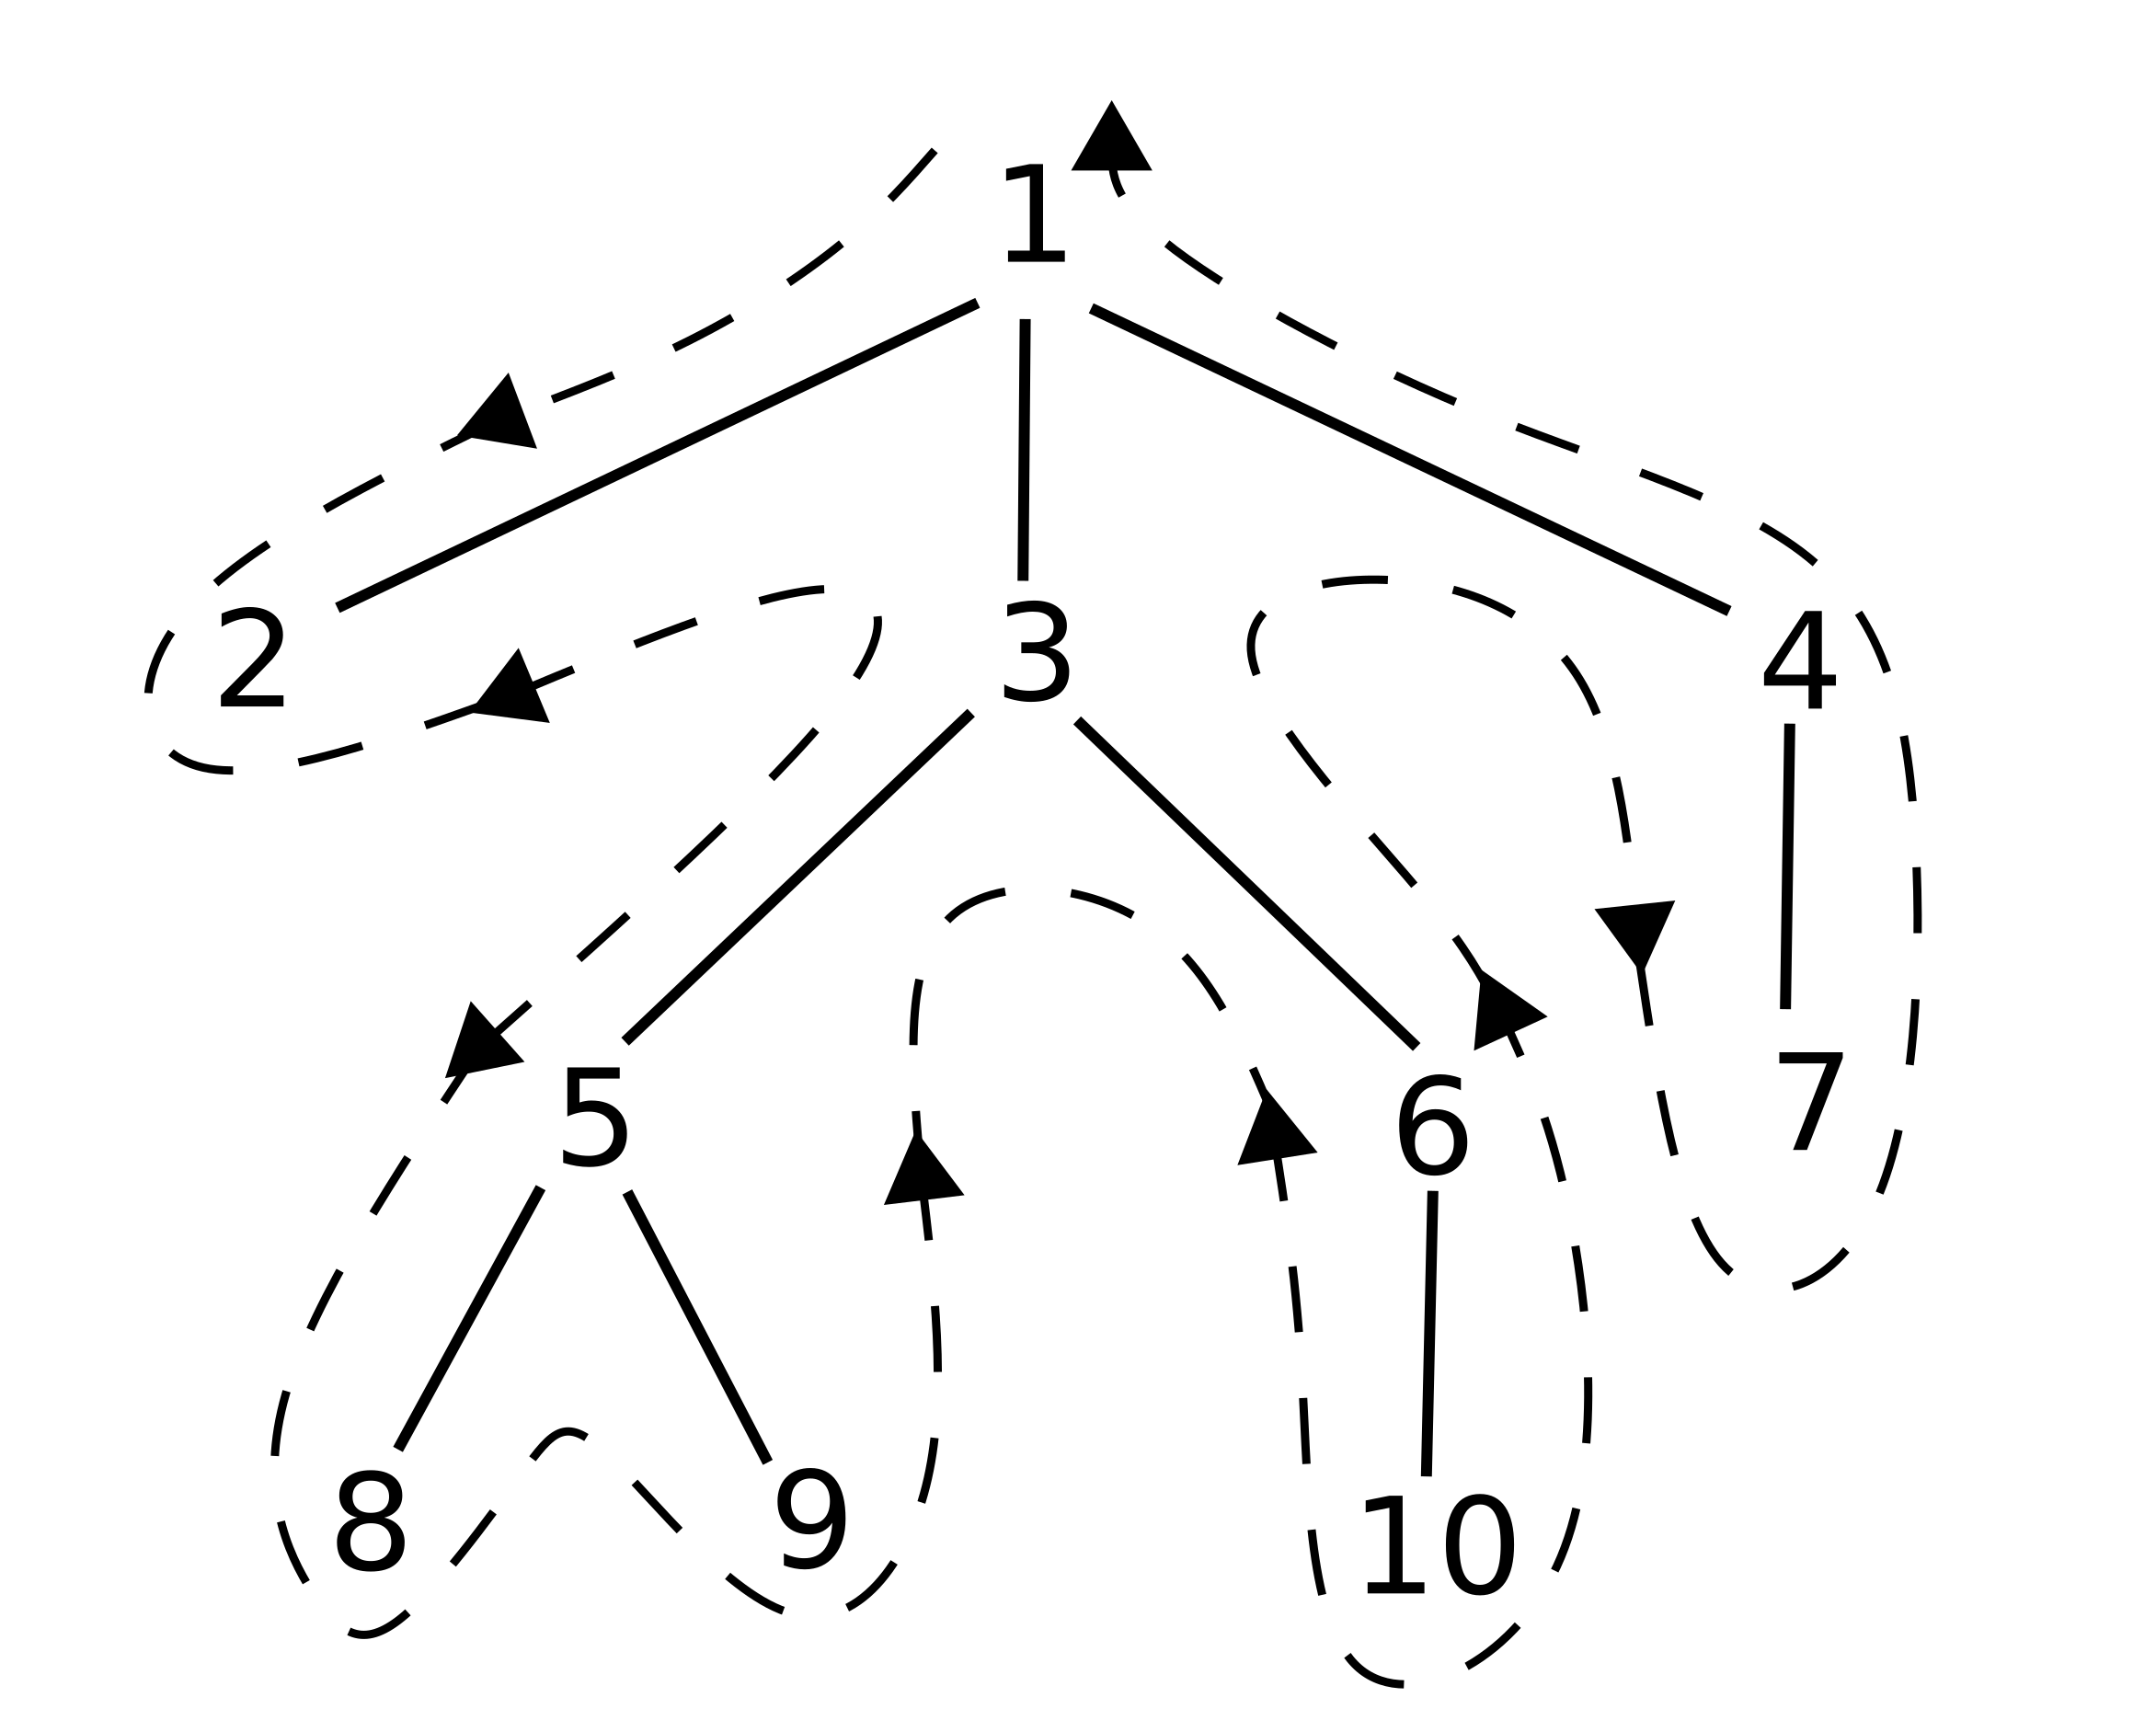
\includegraphics[scale=0.7]{pictures/p79}
\caption{Контур дерева}
\end{figure}

\indent При прямом упорядочивании узлов надо просто записать их в соответствии с
нарисованным контуром. При обратном упорядочивании после записи всех сыновей
переходим к их родителю. При симметричном (внутреннем) упорядочивании
после записи самого правого листа мы переходим не по ветви в направлении к
корню дерева, а к следующему "внутреннему" узлу, который еще не записан.
Например, если на рис. 3.5 узлы 2 и 1 уже записаны, то мы как бы перескакиваем
"залив"\ между узлами 2 и 3 и переходим к узлу 8. Отметим, что при любом
упорядочивании листья всегда записываются в порядке слева направо, при этом
в случае симметричного упорядочивания между сыновьями может быть записан
родитель. $\square$

\subsection*{Помеченные деревья и деревья выражений}
\addcontentsline{toc}{subsection}{ Помеченные деревья и деревья выражений}

\rindex{Дерево!выражений}
\indent Часто бывает полезным сопоставить каждому узлу дерева \textit{метку} (label) или значение,
точно так же, как мы в предыдущей главе сопоставляли элементам списков
определенные значения. Дерево, у которого узлам сопоставлены метки, называется\rindex{Дерево!помеченное}
\textit{помеченным деревом}. Метка узла\rindex{Дерево!метки узлов} — это не имя узла, а значение, которое "хранится"\
в узле. В некоторых приложениях мы даже будем изменять значение метки, поскольку
имя узла сохраняется постоянным. Полезна следующая аналогия: деревосписок,
узел-позиция, метка-элемент.


\indent \textbf{Пример 3.4}. На рис. 3.6 показано дерево с метками, представляющее арифметическое
выражение $(a+b) * (a+c)$, где $n_1, ... , n_7$— имена узлов (метки на рисунке проставлены
рядом с соответствующими узлами). Правила соответствия меток деревьев
элементам выражений следующие.

\begin{enumerate}[topsep=0pt,itemsep=1ex,partopsep=1ex,parsep=1ex]
\item Метка каждого листа соответствует операнду и содержит его значение, например
узел $n_4$
представляет операнд $a$.
\item Метка каждого внутреннего (родительского) узла соответствует оператору. Предположим,
что узел $n$ помечен бинарным оператором в (например, $+$ или $*$) и левый
сын этого узла соответствует выражению $E_1$
, а правый — выражению $E_2$
.
Тогда узел $n$ и его сыновья представляют выражение $(E_1)$ $\theta$ $(E_2)$. Можно удалять
родителей, если это необходимо.
\end{enumerate}

\begin{figure}[ht]
\centering
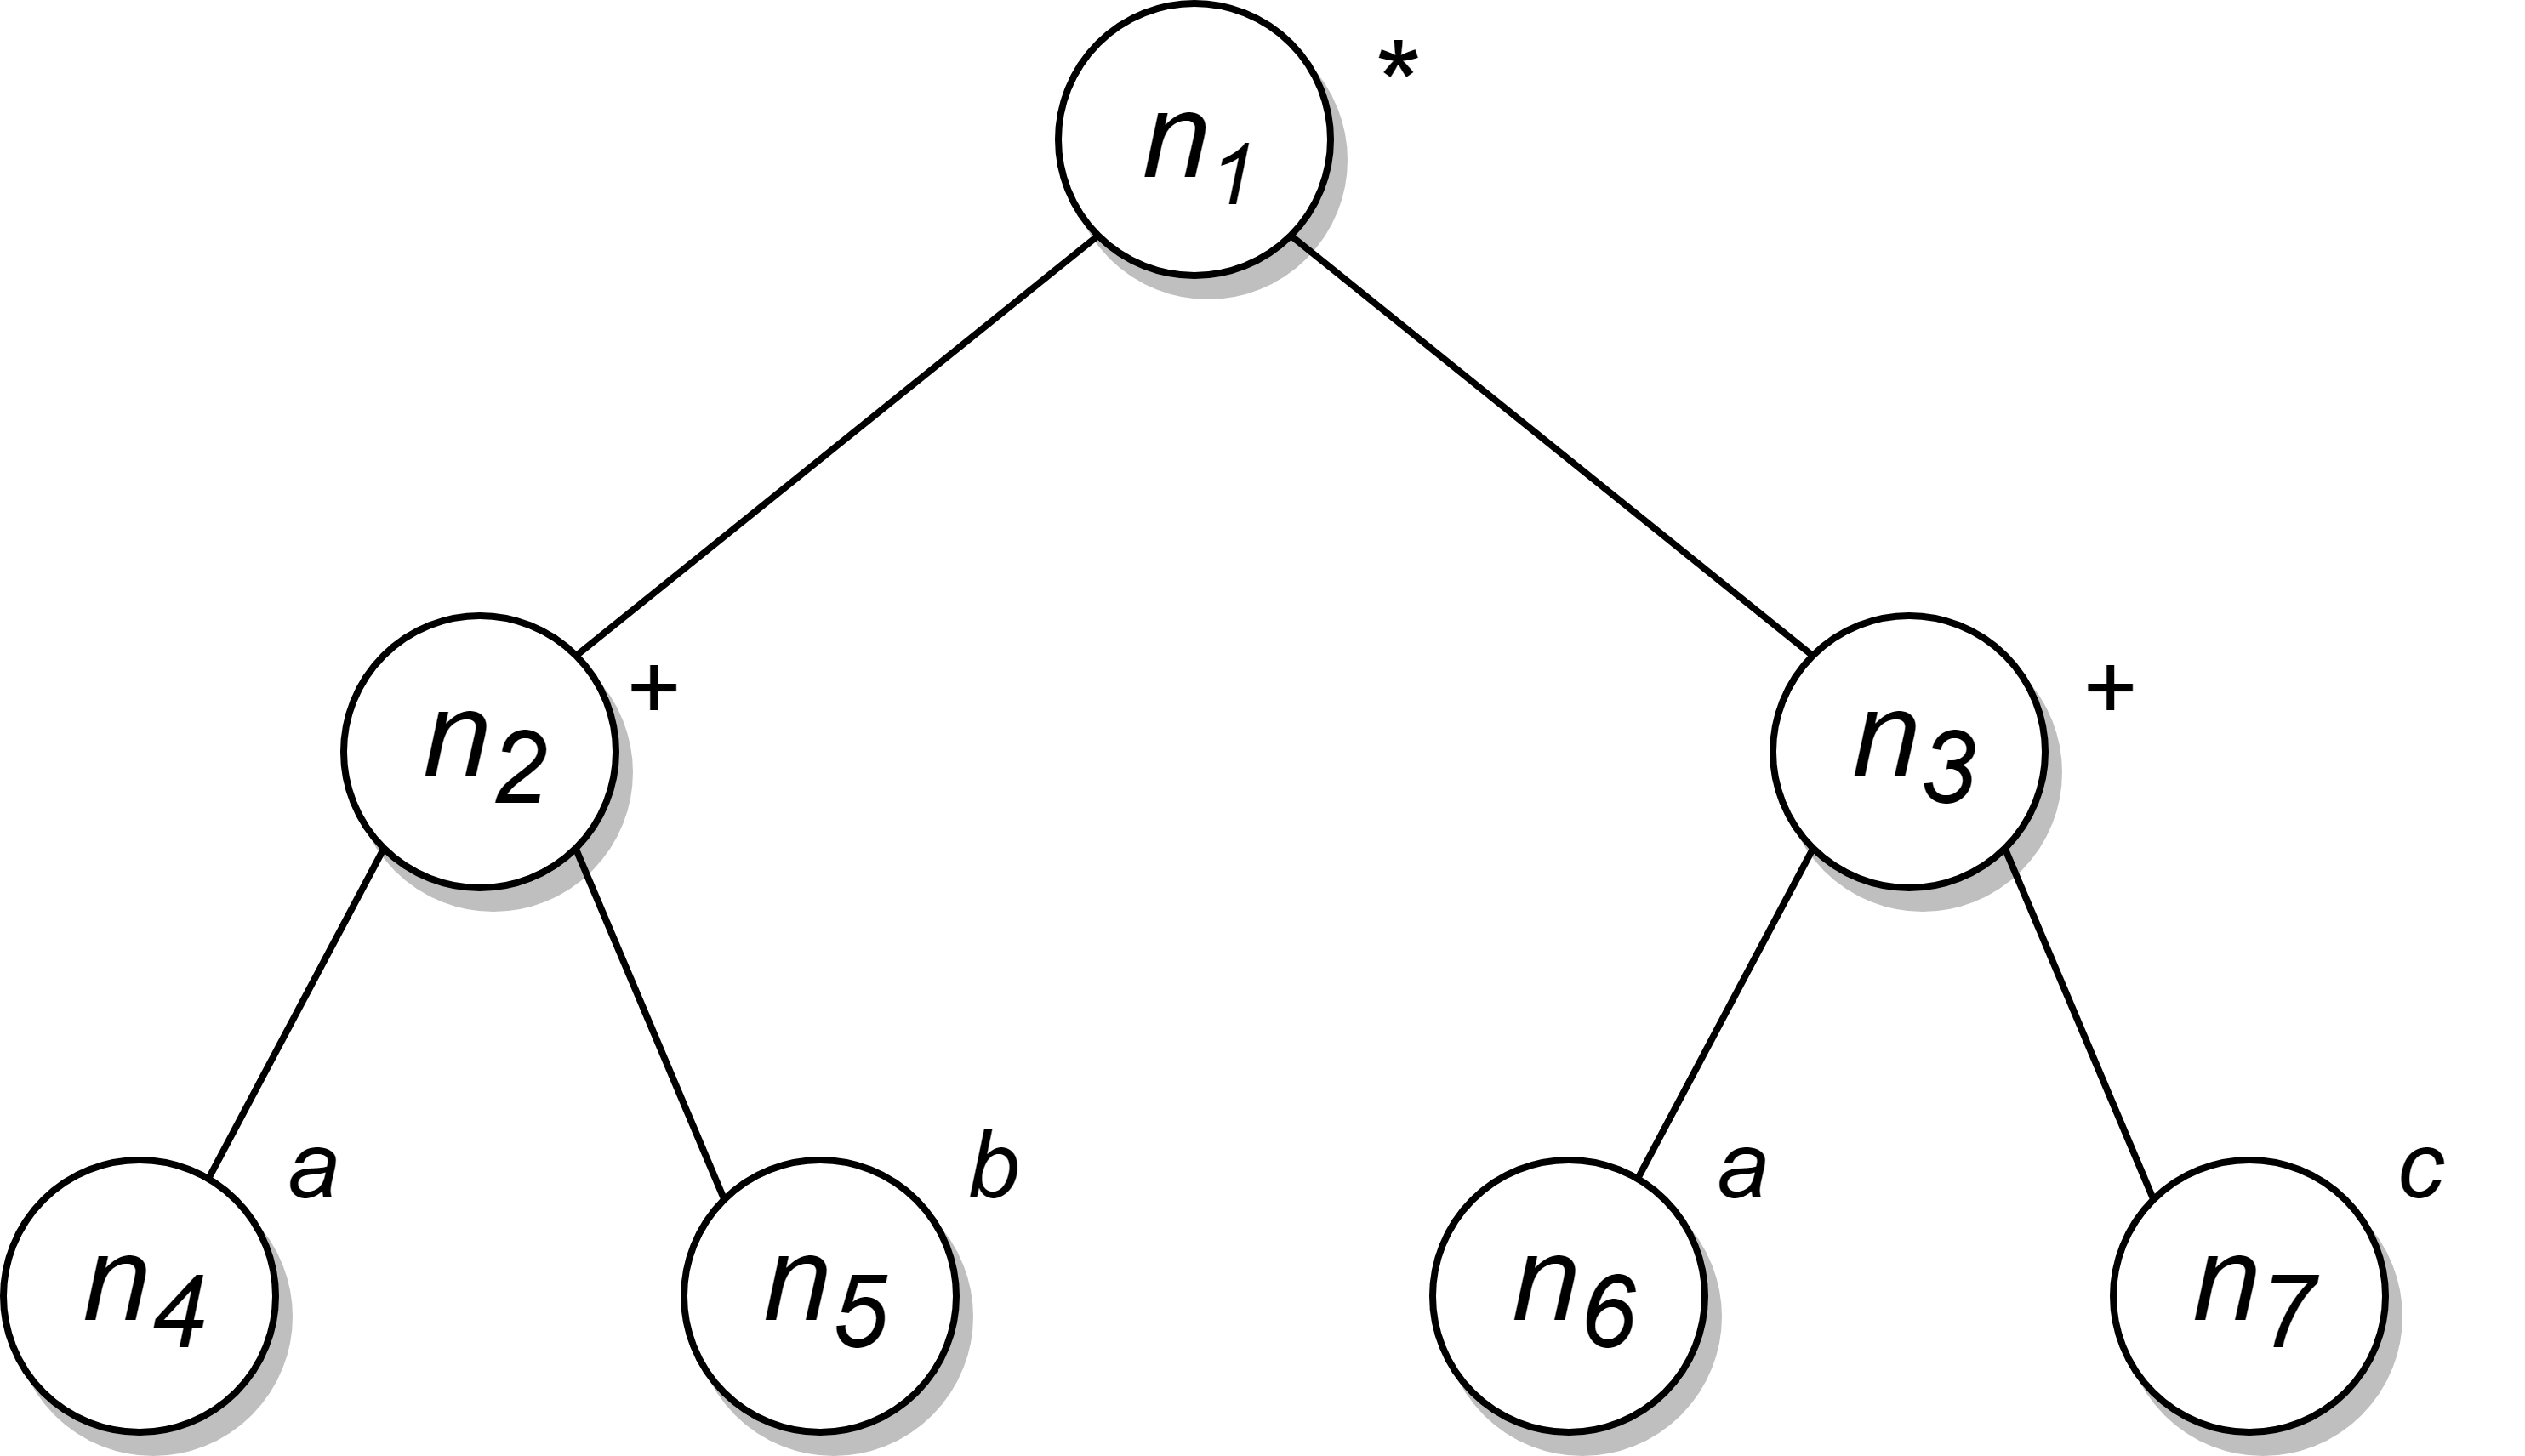
\includegraphics[scale=0.1]{pictures/p80}
\caption{Дерево выражения с метками}
\end{figure} 

\indent Например, узел $n_2$
имеет оператор $+$, а левый и правый сыновья представляют
выражения (операнды) $a$ и $b$ соответственно. Поэтому узел $n_2$
представляет $(a)+(b)$,
т.е. $a+b$. Узел $n_1$
представляет выражение $(a+b)*(a+c)$, поскольку оператор $*$
является меткой узла $n_1$
выражения $a+b$ и $a+c$ представляются узлами $n_2$
и $n_3$ соответственно.$\square$


\indentЧасто при обходе деревьев составляется список не имен узлов, а их меток. В случае
дерева выражений при прямом упорядочивании получаем известную\rindex{Выражения!префиксная форма} \textit{префиксную
форму} выражений, где оператор предшествует и левому, и правому операндам. Для
точного описания префиксной формы выражений сначала положим, что префиксным
выражением одиночного операнда а является сам этот операнд. Далее, префиксная
форма для выражения  $(E_1)$ $\theta$ $(E_2)$, где $\theta$ — бинарный оператор, имеет вид $\theta P_1P_2$
, здесь
$P_1$ и $P_2$
— префиксные формы для выражений $E_1$ и $E_2$
. Отметим, что в префиксных
формах нет необходимости отделять или выделять отдельные префиксные выражения
скобками, так как всегда можно просмотреть префиксное выражение $\theta P_1P_2$
и
определить единственным образом $P_1$ как самый короткий префикс выражения $P_1P_2$.
\indent Например, при прямом упорядочивании узлов (точнее, меток) дерева, показанного
на рис. 3.6, получаем префиксное выражение $*+ab+ac$. Самым коротким корректным
префиксом для выражения $+ab+ac$ будет префиксное выражение узла $n_2: +ab$.


\indent Обратное упорядочивание меток дерева выражений дает так называемое \textit{постфиксное}
(или \textit{польское}) \textit{представление} выражений. Выражение $\theta P_1P_2$
в постфиксной
форме имеет вид $P_1P_2\theta$, где $P_1$
и $P_2$
— постфиксные формы для выражений $E_1$ и $E_2$
соответственно. При использовании постфиксной формы также нет необходимости в
применении скобок, поскольку для любого постфиксного выражения $P_1P_2$
легко проследить
самый короткий суффикс $P_2$
, что и будет корректным составляющим постфиксным
выражением. Например,\rindex{Выражения!постфиксная (польская) форма} постфиксная форма выражения для дерева на
рис. 3.5 имеет вид $ab+ac+*$. Если записать это выражение как $P_1P_2*$, то $P_2$
(т.е. выражение
$ac+$) будет самым коротким суффиксом для $ab+ac+$ и, следовательно, корректным
составляющим постфиксным выражением.


\indent При симметричном обходе дерева выражений\rindex{Выражения!инфиксная форма} получим так называемую \textit{инфиксную
форму} выражения, которая совпадает с привычной "стандартной"\ формой записи
выражений, но также не использует скобок. Для дерева на рис. 3.6 инфиксное
выражение запишется как $a\ +\ b *\ a\ +\ c$. Читателю предлагается разработать алгоритм
обхода дерева выражений, который бы выдавал инфиксную форму выражения
со всеми необходимыми парами скобок.

\subsection*{Вычисление "наследственных"\ данных}
\addcontentsline{toc}{subsection}{ Вычисление "наследственных"\ данных}

\indent Обход дерева в прямом или обратном порядке позволяет получить данные об отношениях
предок-потомок узлов дерева. Пусть функция \textit{postorder(n)} вычисляет позицию
узла $n$ в списке узлов, упорядоченных в обратном порядке. Например, для узлов
$n_2, n_4$ и $n_5$ дерева, представленного на рис. 3.6, значения этой функции будут 3,
1 и 2 соответственно. Определим также функцию \textit{desc(n)}, значение которой равно
числу истинных потомков узла $n$.


\indent Эти функции позволяют выполнить ряд полезных вычислений. Например, все узлы
поддерева с корнем га будут последовательно занимать позиции от \textit{postorder(n) - desc(n)}
до \textit{postorder(n)} в списке узлов, упорядоченных в обратном порядке. Для того чтобы
узел $x$ был потомком узла $y$, надо, чтобы выполнялись следующие неравенства:

\begin{equation*}
postorder(y) - desc(y) \leq  postorder(x) \leq postorder(y)
\end{equation*}

\indent Подобные функции можно определить и для списков узлов, упорядоченных в
прямом порядке.



\section{Абстрактный тип данных \rindex{Абстрактный тип данных!TREE} TREE\rindex{TREE}}


\indent В главе 2 списки, стеки, очереди и отображения получили трактовку как абстрактные
типы данных (АТД). В этой главе рассмотрим деревья как АТД и как
структуры данных. Одно из наиболее важных применений деревьев — это использование
их при разработке реализаций различных АТД. Например, в главе 5 мы покажем,
как можно использовать "дерево двоичного поиска" при реализации АТД, основанных
на математической модели множеств. В следующих двух главах будут представлены
многочисленные примеры применения деревьев при реализации различных
абстрактных типов данных.


\indent В этом разделе мы представим несколько полезных операторов, выполняемых над
деревьями, и покажем, как использовать эти операторы в различных алгоритмах.
Так же, как и в случае списков, можно предложить большой набор операторов, выполняемых
над деревьями. Здесь мы рассмотрим следующие операторы\rindex{Операторы!деревьев}.

\begin{enumerate}[topsep=0pt,itemsep=1ex,partopsep=1ex,parsep=1ex]
\item PARENT\rindex{Оператор!PARENT}($n$, $T$). Эта функция возвращает родителя (parent) узла $n$ в дереве $T$. Если
$n$ является корнем, который не имеет родителя, то в этом случае возвращается $\Lambda$. Здесь $\Lambda$ обозначает "нулевой узел" и указывает на то, что мы выходим за
пределы дерева.

\item LEFTMOST\_CHILD\rindex{Оператор!LEFTMOST\_CHILD}($n, T$). Данная функция возвращает самого левого сына узла $n$ в
дереве $T$. Если $n$ является листом (и поэтому не имеет сына), то возвращается $\Lambda$.

\item RIGHT\_SIBLING\rindex{Оператор!RIGHT\_SIBLING}($n, T$). Эта функция возвращает правого брата узла $n$ в дереве $T$
и значение $\Lambda$, если такового не существует. Для этого находится родитель $p$ узла
$n$ и все сыновья узла $p$, затем среди этих сыновей находится узел, расположенный
непосредственно справа от узла $n$. Например, для дерева на рис. 3.6
LEFTMOST\_CHILD($n_2$) = $n_4$, RIGHT\_SIBLING($n_4$) = $n_5$ и RIGHT\_SIBLING($n_5$) = $\Lambda$.

\item LABEL\rindex{Оператор!LABEL}($n, T$). Возвращает метку узла $n$ дерева $T$. Для выполнения этой функции
требуется, чтобы на узлах дерева были определены метки.

\item CREATEi($v, T_1, T_2, ... , T_i$)\rindex{Оператор!CREATEi} — это обширное семейство "созидающих" функций, которые
для каждого i = 0, 1, 2, ... создают новый корень $r$ с меткой и и далее для этого
корня создает i сыновей, которые становятся корнями поддеревьев $T_1, T_2, ... , T_i$
. Эти
функции возвращают дерево с корнем $r$. Отметим, что если $i = 0$, то возвращается
один узел $r$, который одновременно является и корнем, и листом.

\item  ROOT\rindex{Оператор!ROOT}($T$) возвращает узел, являющимся корнем дерева $T$. Если $T$ — пустое дерево,
то возвращается $\Lambda$.

\item  MAKENULL($T$). Этот оператор делает дерево $T$ пустым деревом.
\end{enumerate}

\indent \textbf{Пример 3.5}. Напишем рекурсивную \textit{PREORDER} и нерекурсивную\\ \textit{NPREORDER}
процедуры обхода дерева в прямом порядке и составления соответствующего \-списка
его меток. Предположим, что для узлов определен тип данных node (узел), так же,
как и для типа данных \textit{TREE} (Дерево), причем \textit{АТД TREE} определен для деревьев с
метками, которые имеют тип данных \textit{labeltype} (тип метки). В листинге 3.2 приведена
рекурсивная процедура, которая по заданному узлу $n$ создает список в прямом порядке
меток поддерева, корнем которого является узел $n$. Для составления списка
всех узлов дерева \textit{Т} надо выполнить вызов \textit{PREORDER(ROOT(T))}.

\begin{lstlisting}[language=C, numbers=none, keepspaces = true, caption = {Рекурсивная процедура обхода дерева в прямом порядке}, captionpos=t] 
    void PREORDER(|\textbf{node}|* root){
        if(root) {
            printf("\%d ", root->data);
            PREORDER(root->left);
            PREORDER(root->right);
        }
    }
\end{lstlisting}

\indentТеперь напишем нерекурсивную процедуру для печати узлов дерева в прямом порядке.
Чтобы совершить обход дерева, используем стек $S$, чей тип данных STACK\rindex{STACK}
уже объявлен как "стек для узлов". Основная идея разрабатываемого алгоритма заключается
в том, что, когда мы дошли до узла и, стек хранит путь от корня до этого
узла, причем корень находится на "дне"\ стека, а узел $n$ — в вершине стека\footnote[1]{ Можно вернуться к разделу 2.6, где обсуждалась реализация рекурсивных процедур с помощью
стека активационных записей. При рассмотрении листинга 3.2 нетрудно заметить, что
активационную запись можно заносить в стек при каждом вызове процедуры PREORDER($n$) и,
это главное, стек будет содержать актнвационные записи для всех предков узла $n$.}.


\indent Один из подходов к реализации обхода дерева в прямом порядке показан на примере
программы NPREORDER в листинге 3.3. Эта программа выполняет два вида
операций, т.е. может находиться как бы в одном из двух режимов. Операции первого
вида (первый режим) осуществляют обход по направлению к потомкам самого левого
еще не проверенного пути дерева до тех пор, пока не встретится лист, при этом выполняется
печать узлов этого пути и занесение их в стек.


\indent Во втором режиме выполнения программы осуществляется возврат по пройденному
пути с поочередным извлечением узлов из стека до тех пор, пока не встретится
узел, имеющий еще "не описанного"\ правого брата. Тогда программа опять переходит
в первый режим и исследует новый путь, начиная с этого правого брата.


\indent Программа начинается в первом режиме с нахождения корня дерева и определения,
является ли стек пустым. В листинге 3.3 показан полный код этой программы. $\square$ 

\begin{lstlisting}[language=C, numbers=none, caption = {Нерекурсивная процедура обхода дерева в прямом порядке}, captionpos=t] 
    int NPREORDER(|\textbf{Tree}|* T){
        |\textbf{node}| m;  //| переменная для временного хранения узлов| 
        |\textbf{stack}| S; //| стек узлов, хранящий путь от корня до|
        MAKENULL(S);        //| родителя $TOP(S)$ текущего узла $m$|
        m = ROOT(T);
        while(1){
            if(m != NULL){
                printf("\%d", LABEL(m, T));
                PUSH(m, S); //| исслеование самого левого узла $m$|
            }
            else{ //| завершена проверка пути, содержащегося в стеке|
                if(EMPTY(S))
                    return;
                m = RIGHT_SIBLING(TOP(S), T);
                POP(S);
            }
        } 
    }
\end{lstlisting}

\section{Реализация деревьев}\rindex{Реализация!деревьев}

В этом разделе мы представим несколько основных реализаций деревьев и обсудим
их возможности для поддержки операторов, введенных в разделе 3.2.

\subsection*{Представление деревьев с помощью массивов}\rindex{Дерево!представление посредством массива}
\addcontentsline{toc}{subsection}{ Представление деревьев с помощью массивов}

\indent Пусть $T$ — дерево с узлами 1, 2, ... , $n$. Возможно, самым простым представлением
дерева $T$, поддерживающим оператор PARENT (Родитель), будет линейный массив $A$,
где каждый элемент $A[i]$ является указателем или курсором на родителя узла $i$. Корень
дерева $T$ отличается от других узлов тем, что имеет нулевой указатель или указатель
на самого себя как на родителя. Мы будем использовать схему с курсорами, тогда $A[i] = j$, если узел $j$
является родителем узла $i$, и $A[i] = 0$, если узел $i$ является корнем.

\begin{figure}[ht]
\centering
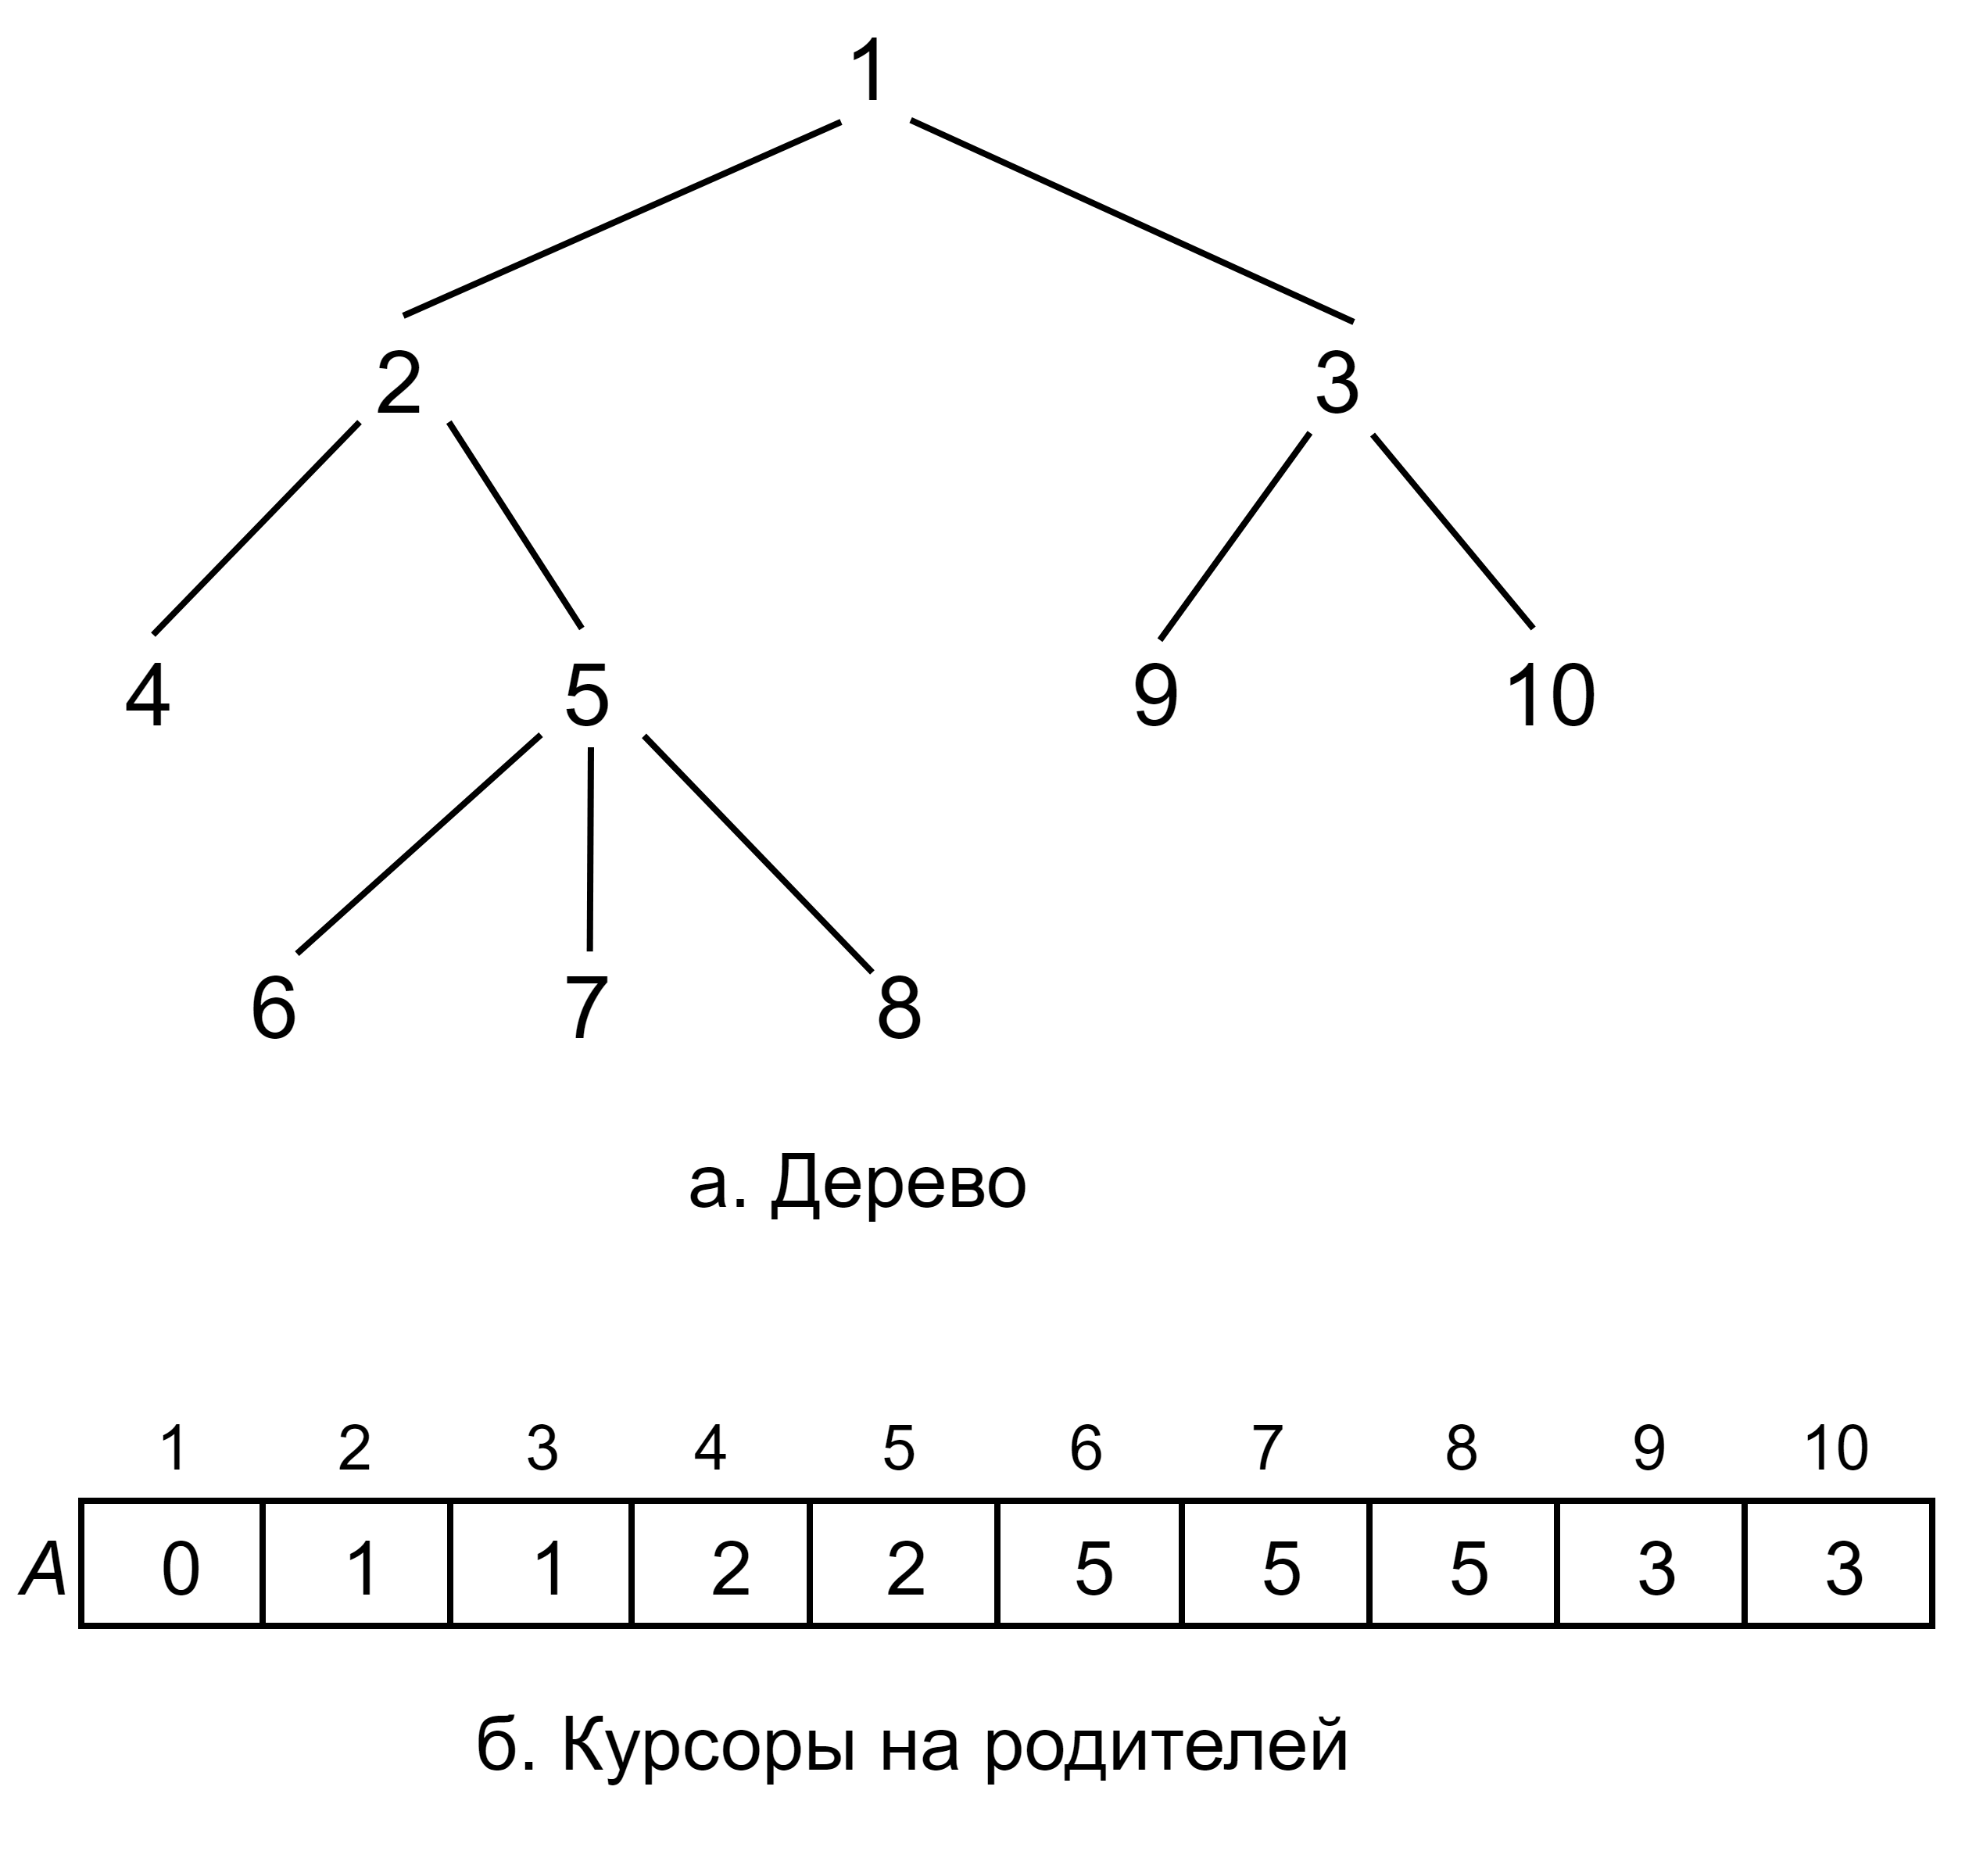
\includegraphics[scale=0.12]{pictures/p83}
\caption{Дерево и курсоры на родителей}
\end{figure}

\indent Данное представление использует то свойство деревьев, что каждый узел, отличный
от корня, имеет только одного родителя. Используя это представление, родителя любого
узла можно найти за фиксированное время. Прохождение по любому пути, т.е. переход
по узлам от родителя к родителю, можно выполнить за время, пропорциональное
количеству узлов пути. Для реализации оператора LABEL можно использовать другой
массив $L$, в котором элемент $L[i]$ будет хранить метку узла $i$, либо объявить элементы
массива $A$ записями, состоящими из целых чисел (курсоров) и меток.\


\indent \textbf{Пример 3.6}. На рис. 3.7 показаны дерево и массив $A$ курсоров на родителей этого
дерева. $\square$ 


\indent Использование указателей или курсоров на родителей не помогает в реализации
операторов, требующих информацию о сыновьях. Используя описанное представление,
крайне тяжело для данного узла $n$ найти его сыновей или определить
его высоту. Кроме того, в этом случае невозможно определить порядок сыновей
узла (т.е. какой сын находится правее или левее другого сына). Поэтому нельзя
реализовать операторы, подобные LEFTMOST\_CHILD и RIGHT\_SIBLING. Можно
ввести искусственный порядок нумерации узлов, например нумерацию сыновей в
возрастающем порядке слева направо. Используя такую нумерацию, можно реализовать
оператор RIGHT\_SIBLING, код для этого оператора приведен в листинге
3.4. Для задания типов данных node (узел) и TREE (Дерево) используется
следующее объявление:

\begin{lstlisting}[language=C, numbers=none]*
    typedef integer node;
    typedef node[maxnodes] TREE;
\end{lstlisting}

\indent В этой реализации мы предполагаем, что нулевой узел $\Lambda$ представлен 0.

\begin{lstlisting}[language=C, numbers=none, caption = {Оператор определения правого брата}, captionpos=t] 
    |\textbf{node}|* RIGHT_SIBLING(|\textbf{node}| n; |\textbf{Tree}|* T){
        |\textbf{node}| i, parent;
        parent = T[n];
        for(i = n+1; i = maxnodes; i++){
            if(T[i] == parent)
                return i;
            return 0; //| правый брат не найден|
        } 
    }
\end{lstlisting}

\subsection*{Представление деревьев с использованием списков сыновей}\rindex{Дерево!представление посредством списоков сыновей}
\addcontentsline{toc}{subsection}{ Представление деревьев с использованием списков сыновей}

\indent Важный и полезный способ представления деревьев состоит в формировании для
каждого узла списка его сыновей. Эти списки можно представить любым методом,
описанным в главе 2, но, так как число сыновей у разных узлов может быть разное,
чаще всего для этих целей применяются связанные списки.


\indent На рис. 3.8 показано, как таким способом представить дерево, изображенное на
рис. 3.7, а. Здесь есть массив ячеек заголовков, индексированный номерами (они же
имена) узлов. Каждый заголовок $(header)$ указывает на связанный список, состоящий
из "элементов" - узлов. Элементы списка $header[i]$ являются сыновьями узла $i$, например
узлы 9 и 10 — сыновья узла 3.


\indent Прежде чем разрабатывать необходимую структуру данных, нам надо в терминах
абстрактного типа данных LIST \rindex{LIST} (список узлов) сделать отдельную реализацию списков
сыновей и посмотреть, как эти абстракции согласуются между собой. Позднее
мы увидим, какие упрощения можно сделать в этих реализациях. Начнем со следующих
объявлений типов:

\begin{lstlisting}[language=C, numbers=none]*
    typedef int node; 
    typedef /*|соотв опис|*/ LIST; 
    typedef /*|соотв опис|*/ position; 
    typedef struct{ 
        LIST header[maxnodes]; 
        labeltype labels[maxnodes]; 
        node root; 
    }TREE;
\end{lstlisting}

\begin{figure}[ht]
\centering
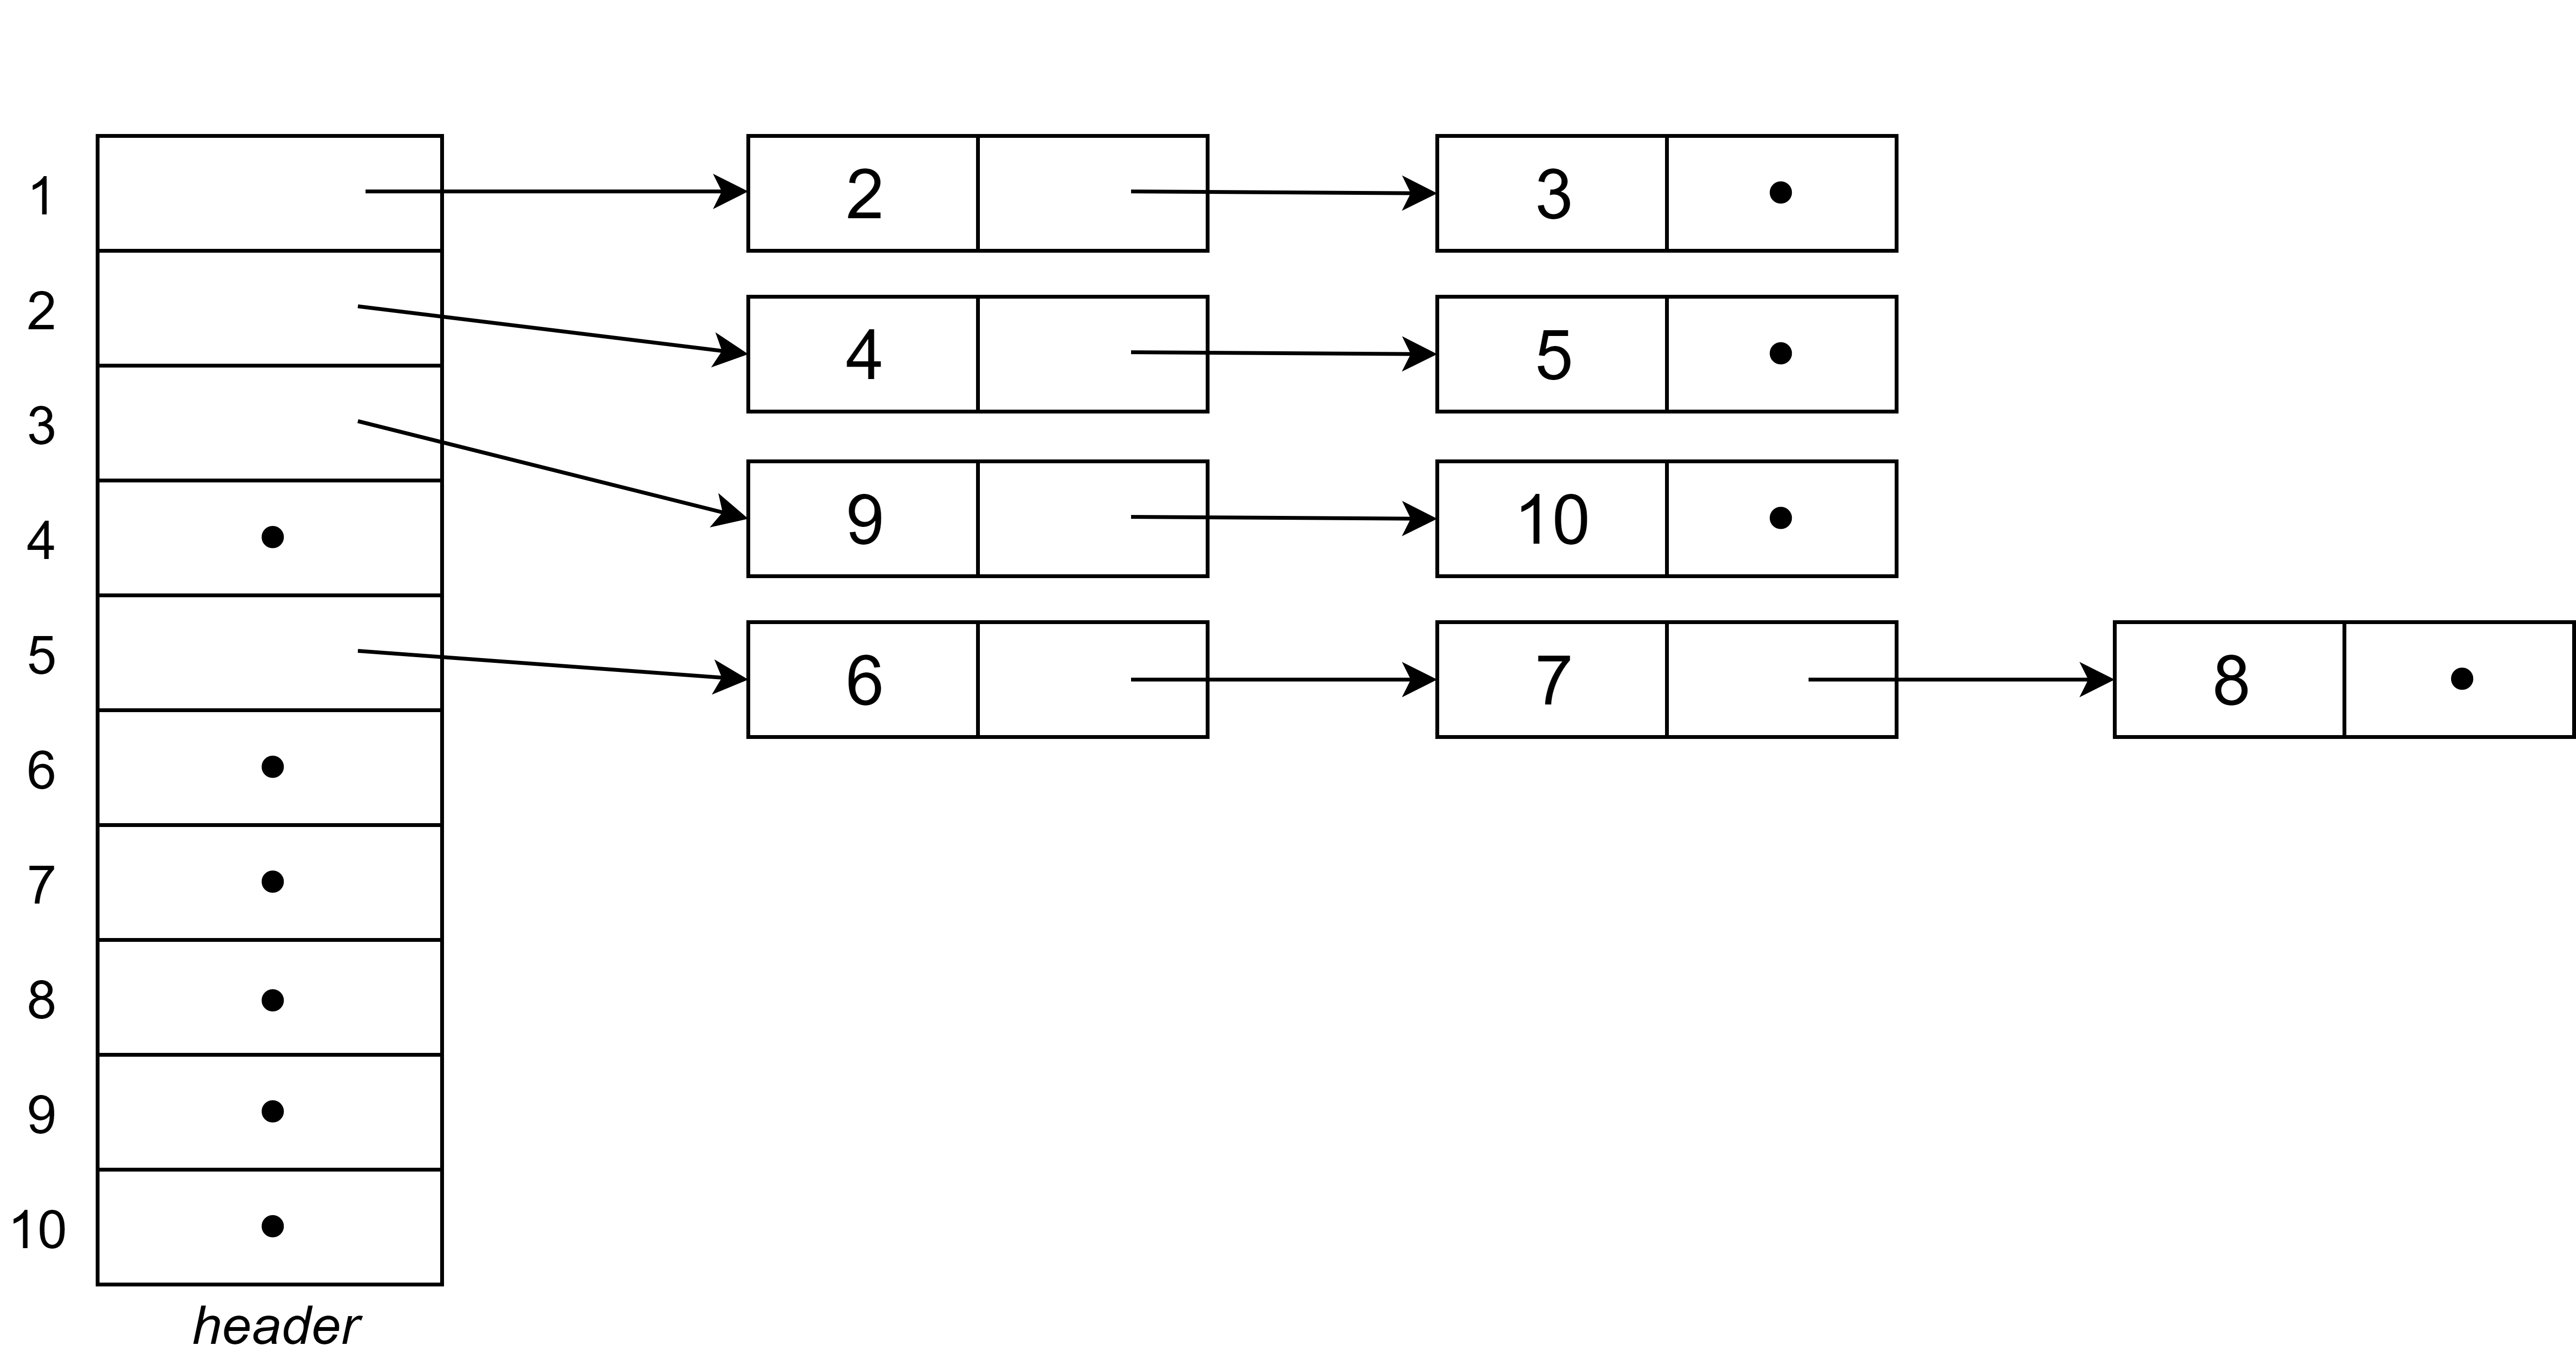
\includegraphics[scale=0.08]{pictures/p85}
\caption{Представление дерева с помощью связанных списков}
\end{figure}


\indent Мы предполагаем, что корень каждого дерева хранится отдельно в поле $root$
(корень). Для обозначения нулевого узла используется 0.


\indent В листинге 3.5 представлен код функции LEFTMOST\_CHILD. Читатель в качестве
упражнения может написать коды других операторов.

\rindex{Программа!LEFTMOST_CHILD}
\begin{lstlisting}[language=C, numbers=none, caption = { Функция нахождения самого левого сына}, captionpos=t] 
    |\textbf{node}|* LEFTMOST_CHILD(|\textbf{node}| n, |\textbf{Tree}|* T){
        |\textbf{List}| L; //| скоропись для списка сыновей узла $n$|
        L = T.header[n];
        if(EMPTY(L)) //| $n$ является листом|
            return 0;
        else
            return RETRIEVE(FIRST(L), L);
    }
\end{lstlisting}

\indent Теперь представим конкретную реализацию списков, где типы LIST и position
имеют тип целых чисел, последние используются как курсоры в массиве записей
$cellspace$ (область ячеек).

\begin{lstlisting}[language=C, numbers=none]*
    typedef /*|соотв опис|*/ record; 
    typedef struct{ 
        record cellspace[maxnodes];
        int node;
        int next;
    } List;
\end{lstlisting}

\indent Для упрощения реализации можно положить, что списки сыновей не имеют ячеек
заголовков. Точнее, мы поместим $T.header[n]$ непосредственно в первую ячейку
списка, как показано на рис. 3.8. В листинге 3.6 представлен переписанный (с учетом
этого упрощения) код функции LEFTMOST\_CHILD, а также показан код функции
PARENT, использующий данное представление списков. Эта функция более
трудна для реализации, так как определение списка, в котором находится заданный
узел, требует просмотра всех списков сыновей.

\rindex{Реализация!операторов деревьев}
\begin{lstlisting}[language=C, numbers=none, keepspaces = true, caption = {Функции, использующие представление деревьев посредством связанных списков}] 
    |\textbf{node}|* LEFTMOST_CHILD(|\textbf{node}| n, |\textbf{Tree}| *T){ 
    // Возвращает самого левого сына узла n дерева T
        int L; //курсор на начало списка сыновей узла n
        L = T.header[n];
        if(L == 0) // n является листом
            return 0;
        else
            return cellspace[L].node;
    }

    |\textbf{node}|* PARENT(|\textbf{node}| n, |\textbf{Tree*}| T){ 
    // Возвращает родителя узла n дерева T
        |\textbf{node}| p; // пробегает список сыновей p
        |\textbf{position}| i;
        for(p = 1; p = maxnodes; p++){
            i = T.header[p];
            while(i != 0){
                if(cellspace[i].node == n)
                    return p;
                else
                    i = cellspace[i].next;
            }
        }
        return 0;
    }
\end{lstlisting}

\subsection*{Представление левых сыновей и правых братьев}
\addcontentsline{toc}{subsection}{ Представление левых сыновей и правых братьев}

\indent Среди прочих недостатков описанная выше структура данных не позволяет также
с помощью операторов $CREATEi$ создавать большие деревья из малых. Это является
следствием того, что все деревья совместно используют массив $cellspace$ для представления
связанных списков сыновей; по сути, каждое дерево имеет собственный
массив заголовков для своих узлов. А при реализации, например, оператора $CREATE2(V, T_1, T_2) $надо скопировать деревья $T_1$ и $T_2$
в третье дерево и добавить новый
узел с меткой v и двух его сыновей — корни деревьев $T_1$ и $T_2$.


\indent Если мы хотим построить большое дерево на основе нескольких малых, то желательно,
чтобы все узлы всех деревьев располагались в одной общей области. Логическим
продолжением представления дерева, показанного на рис. 3.8, будет замена
массива заголовков на отдельный массив $nodespace$ (область узлов), содержащий записи
с произвольным местоположением в этом массиве. Содержимое поля $header$
этих записей соответствует "номеру"\ узла, т.е. номеру записи в массиве $cellspace$, в свою очередь поле $node$ массива $cellspace$ теперь является курсором для массива
$nodespace$, указывающим позицию узла. Тип TREE в этой ситуации просто курсор в
массиве $nodespace$, указывающий позицию корня.


\indent \textbf{Пример 3.7.} На рис. 3.9, а показано дерево, а на рис. 3.9, б — структура данных,
где узлы этого дерева, помеченные как А, В, С и. D, размещены в произвольных позициях
массива $nodespace$. В массиве $cellspace$ также в произвольном порядке размещены
списки сыновей.$\square$ 

\begin{figure}[ht]
\centering
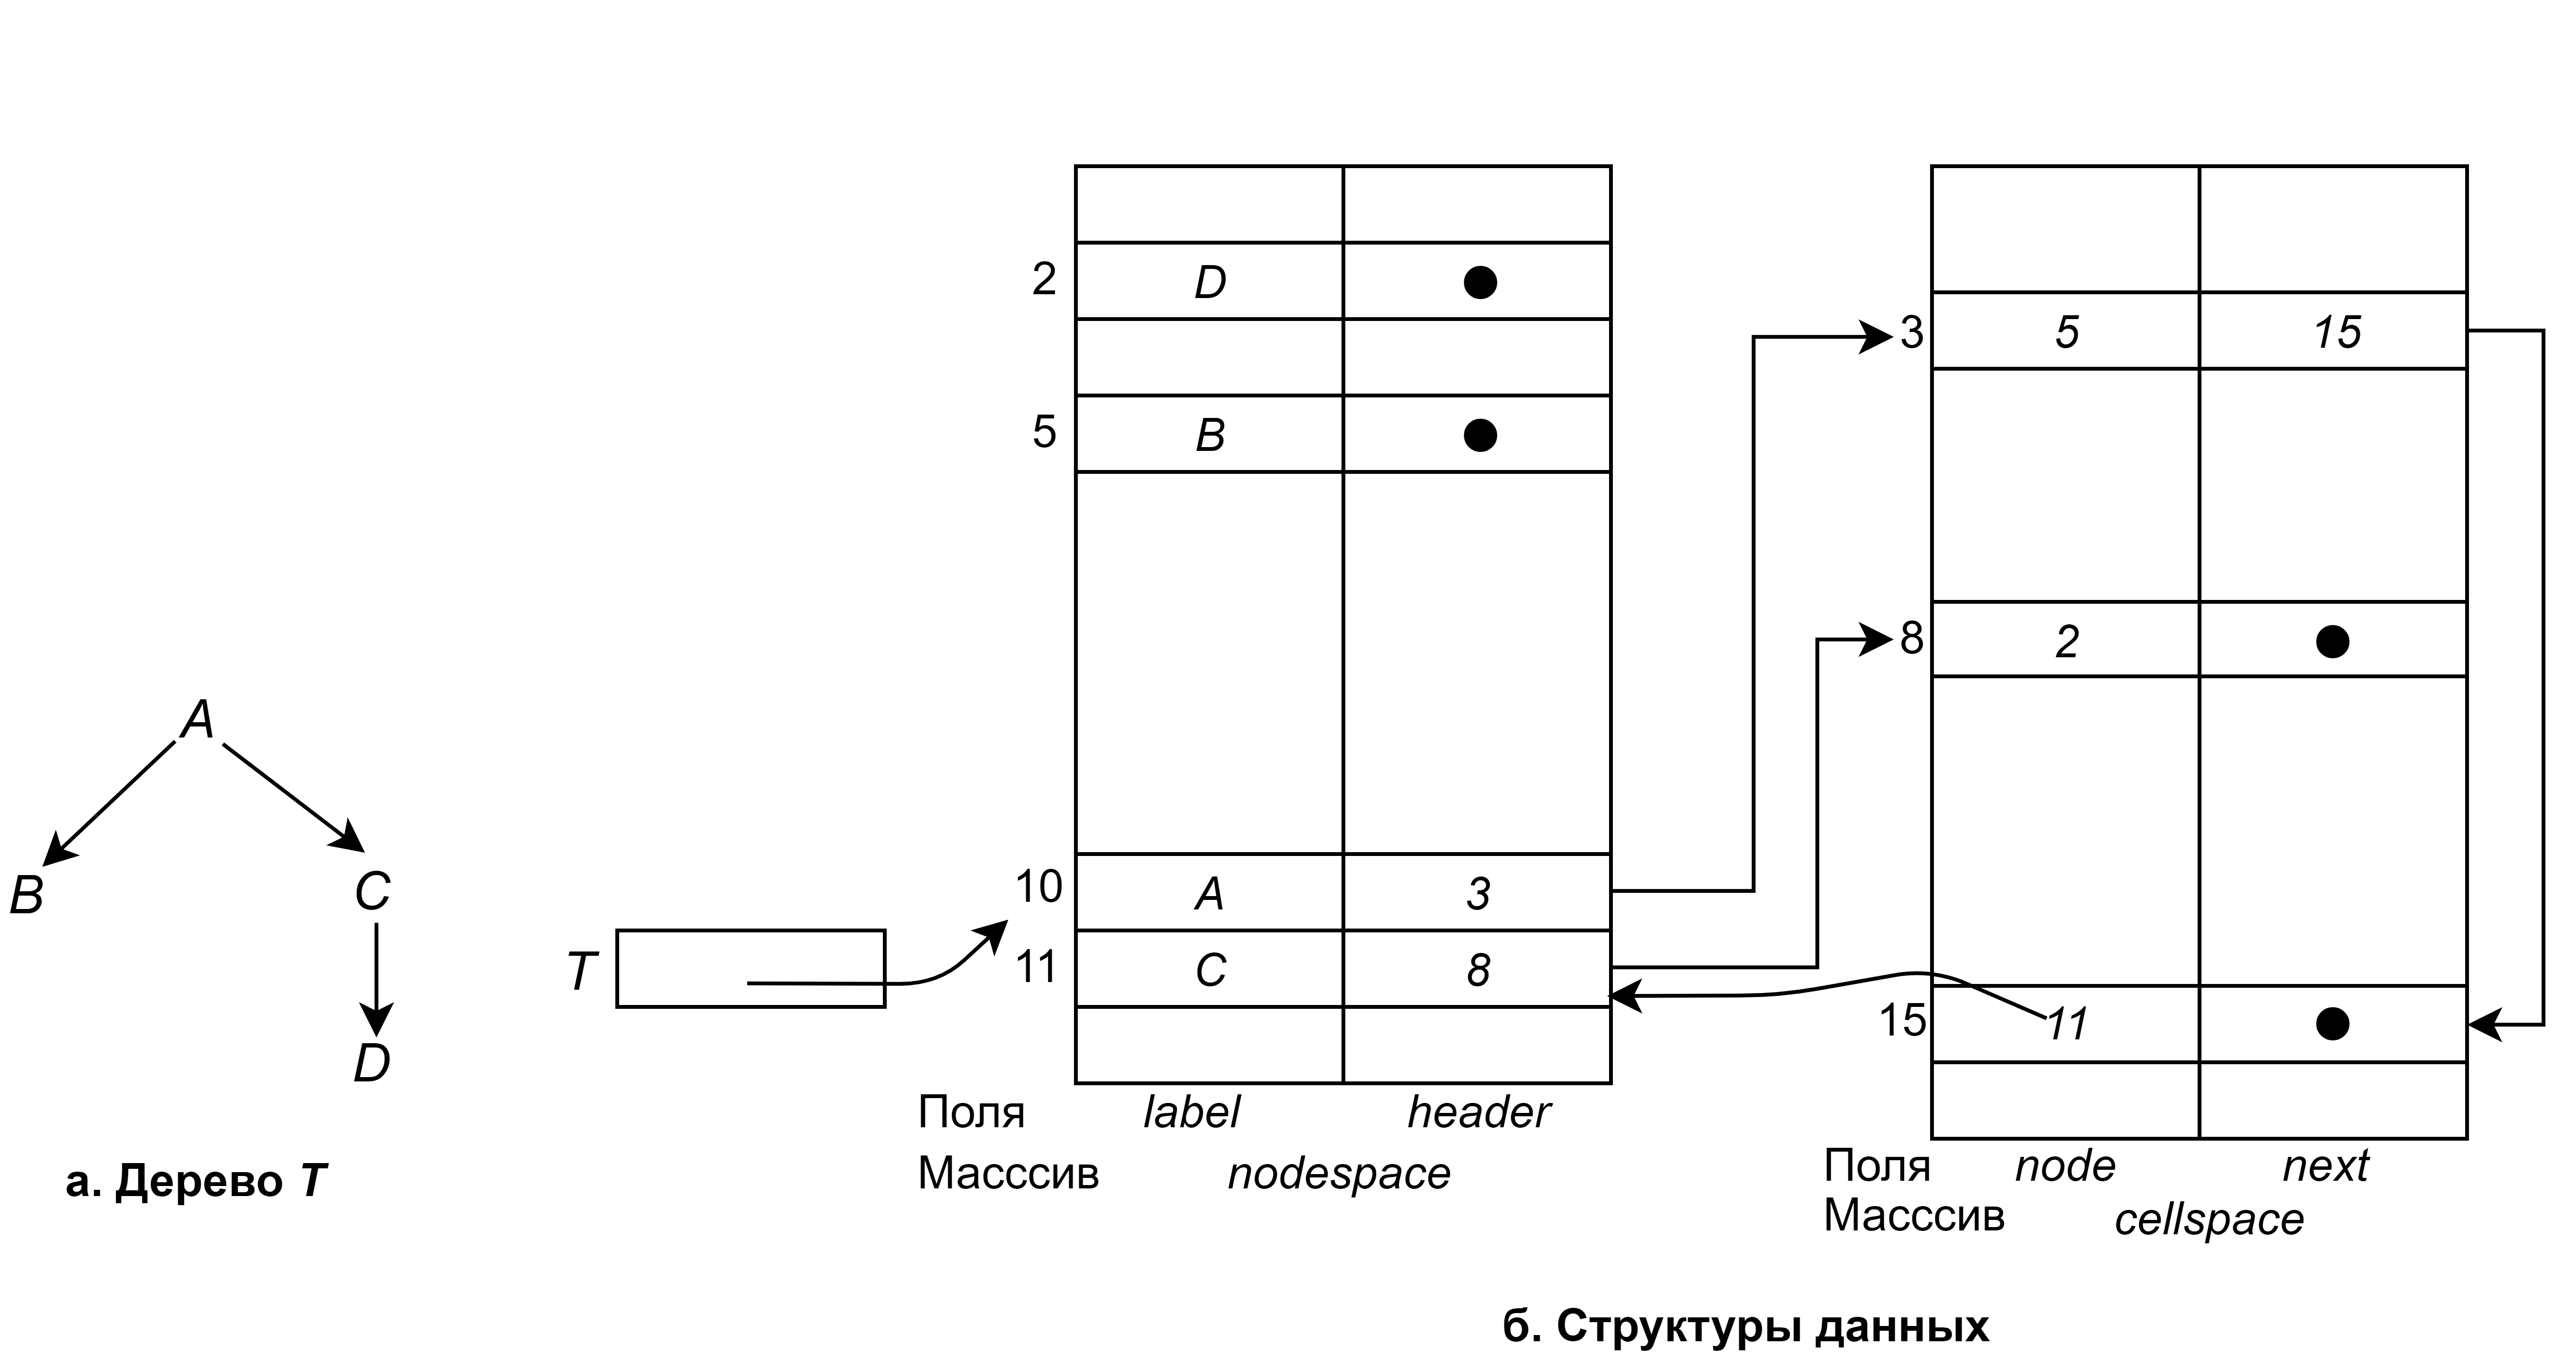
\includegraphics[scale=0.08]{pictures/p87}
\caption{Структура данных для дерева, использующая связанные списки}
\end{figure}

\indent Структура данных, показанная на рис. 3.9, б, уже подходит для того, чтобы организовать
слияние деревьев с помощью операторов CREATEi. Но и эту структуру
можно значительно упростить. Для этого заметим, что цепочка указателей поля $next$
массива $cellspace$ перечисляет всех правых братьев.

\indent Используя эти указатели, можно найти самого левого сына следующим образом.
Предположим, что $cellspace[i].node = n$. (Повторим, что "имя"\ узла, в отличие от его
метки, является индексом в массиве $nodespace$ и этот индекс записан в поле $cellspace[i].node$.)
Тогда указатель $nodespace[n].header$ указывает на ячейку самого левого
сына узла $n$ в массиве $cellspace$, поскольку поле $node$ этой ячейки является именем
этого узла в массиве $nodespace$.

\indent Можно упростить структуру, если идентифицировать узел не с помощью индекса
в массиве $nodespace$, а с помощью индекса ячейки в массиве $cellspace$, который соответствует
данному узлу как сыну. Тогда указатель $next$ (переименуем это поле в
$right\_sibling$ — правый брат) массива $cellspace$ будет точно указывать на правого брата,
а информацию, содержащуюдя в массиве nodespace, можно перенести в новое поле
$leftmost\_child$ (самый левый сын) массива $cellspace$. Здесь тип TREE является целочисленным
типом и используется как курсор в массиве cellspace, указывающий на
корень дерева. Массив $cellspace$ можно описать как следующую структуру:

\begin{lstlisting}[language=C, numbers=none]*
typedef /*соотв опис*/ record; 
typedef struct{ 
record cellspace[maxnodes];
labeltype label;
int tight_sibling;
int leftmost_child;
}cellspace;
\end{lstlisting}

\indent \textbf{Пример 3.8}. Новое представление для дерева, показанного на рис. 3.9, а, схематически
изображено на рис. 3.10. Узлы дерева расположены в тех же ячейках массива,
что и на рис. 3.9, б.$\square$

\begin{figure}[ht]
\centering
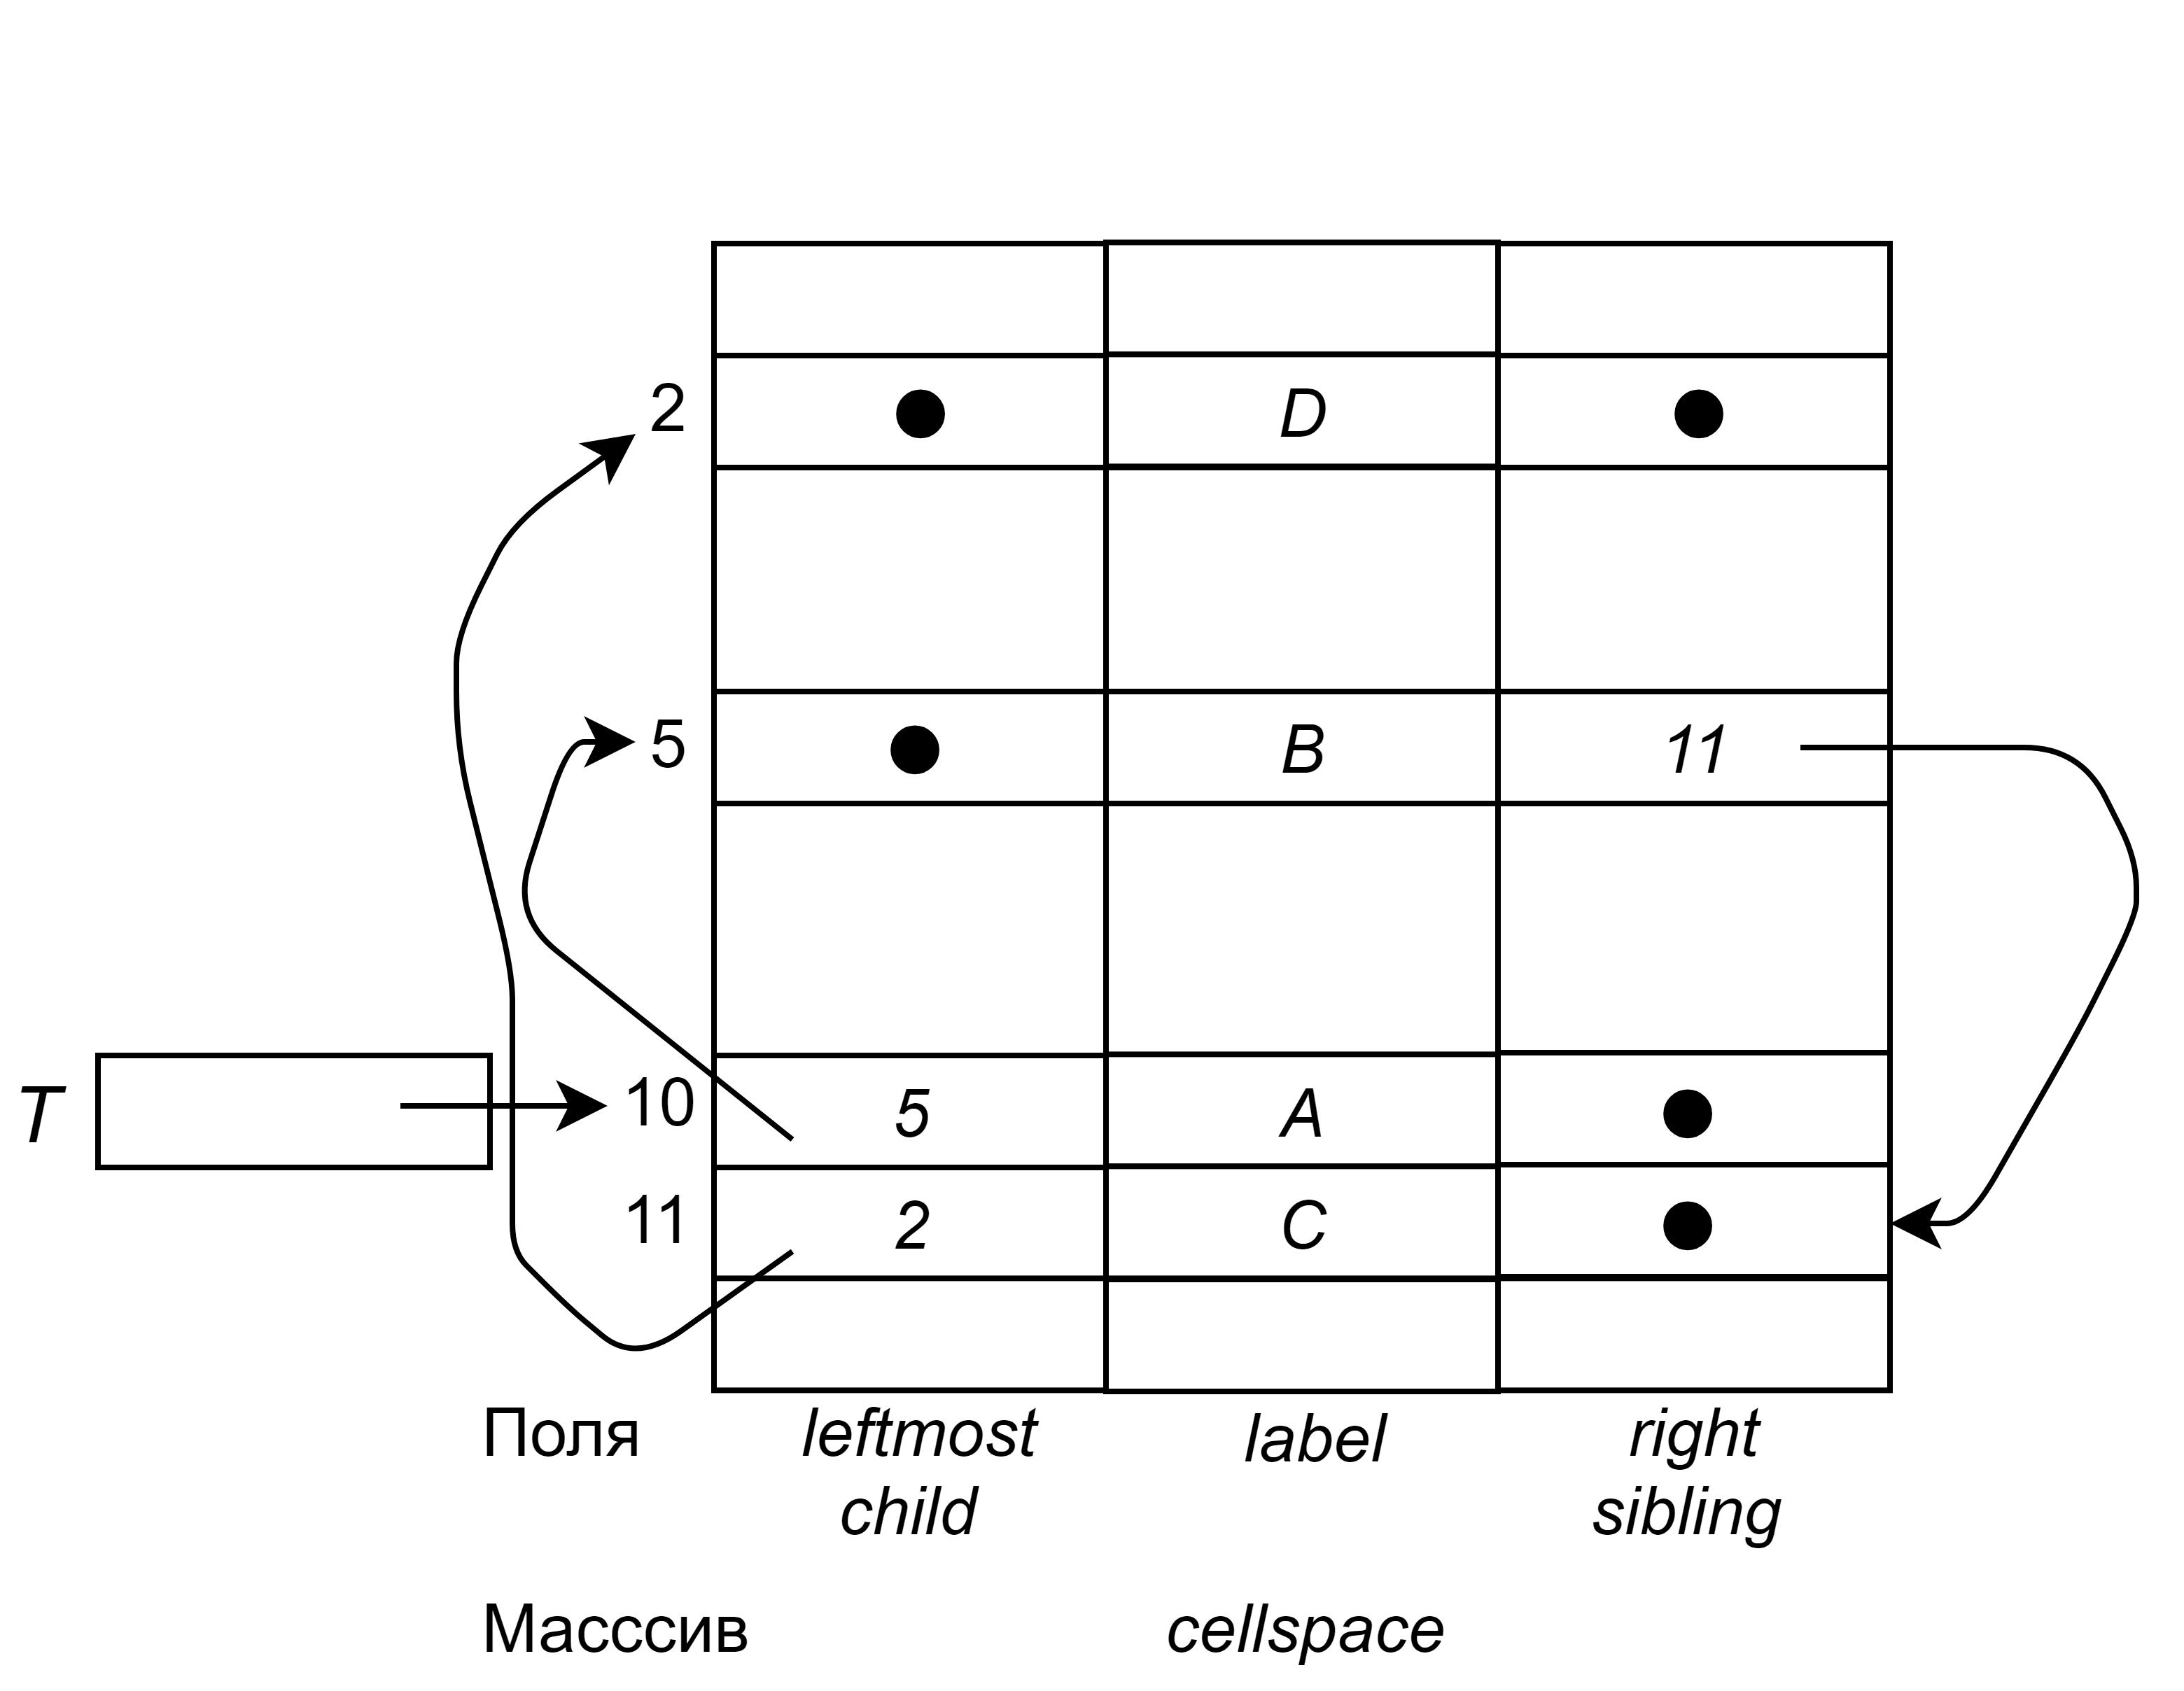
\includegraphics[scale=0.095]{pictures/p88}
\caption{ Представление дерева посредством левых сыновей и правых братьев}
\end{figure}

\indent Используя описанное представление, все операторы, за исключением PARENT,
можно реализовать путем прямых вычислений. Оператор PARENT требует просмотра
всего массива $cellspace$. Если необходимо эффективное выполнение оператора
PARENT, то можно добавить четвертое поле в массив $cellspace$ для непосредственного
указания на родителей.

\indent В качестве примера операторов, использующих структуры данных рис. 3.10, напишем
код функции CREATE2\rindex{Программа!CREATE2}, показанный в листинге 3.7. Здесь мы предполагаем,
что неиспользуемые ячейки массива $cellspace$ связаны в один свободный список, который
в листинге назван как $avail$, и ячейки этого списка связаны посредством поля
$right\_sibling$. На рис. 3.11 показаны старые (сплошные линии) и новые (пунктирные
линии) указатели в процессе создания нового дерева.

\newpage
\begin{lstlisting}[language=C, captionpos=t, numbers=none, caption = {Функция CREATE2}]
typedef /* соотв. опис. */ root;
int CREATE2(root v, int T1, int T2){
	| // Возвращает новое дерево с корнем v и поддеревьями T1 и T2|
	int temp; |//  хранит индекс первой свободной ячейки для корня нового дерева|
	temp = avail;
	avail = cellspace[avail].right_sibling
	cellspace[temp].leftmost_child = 21;
	cellspace[temp].label = v;
	cellspace[temp].right_sibling = 0;
	cellspace[T1].right_sibling = T2;
	cellspace[T2].right_sibling = 0; |// необязательный оператор|
	
	return temp;
}
\end{lstlisting}

\begin{figure}[ht]
\centering
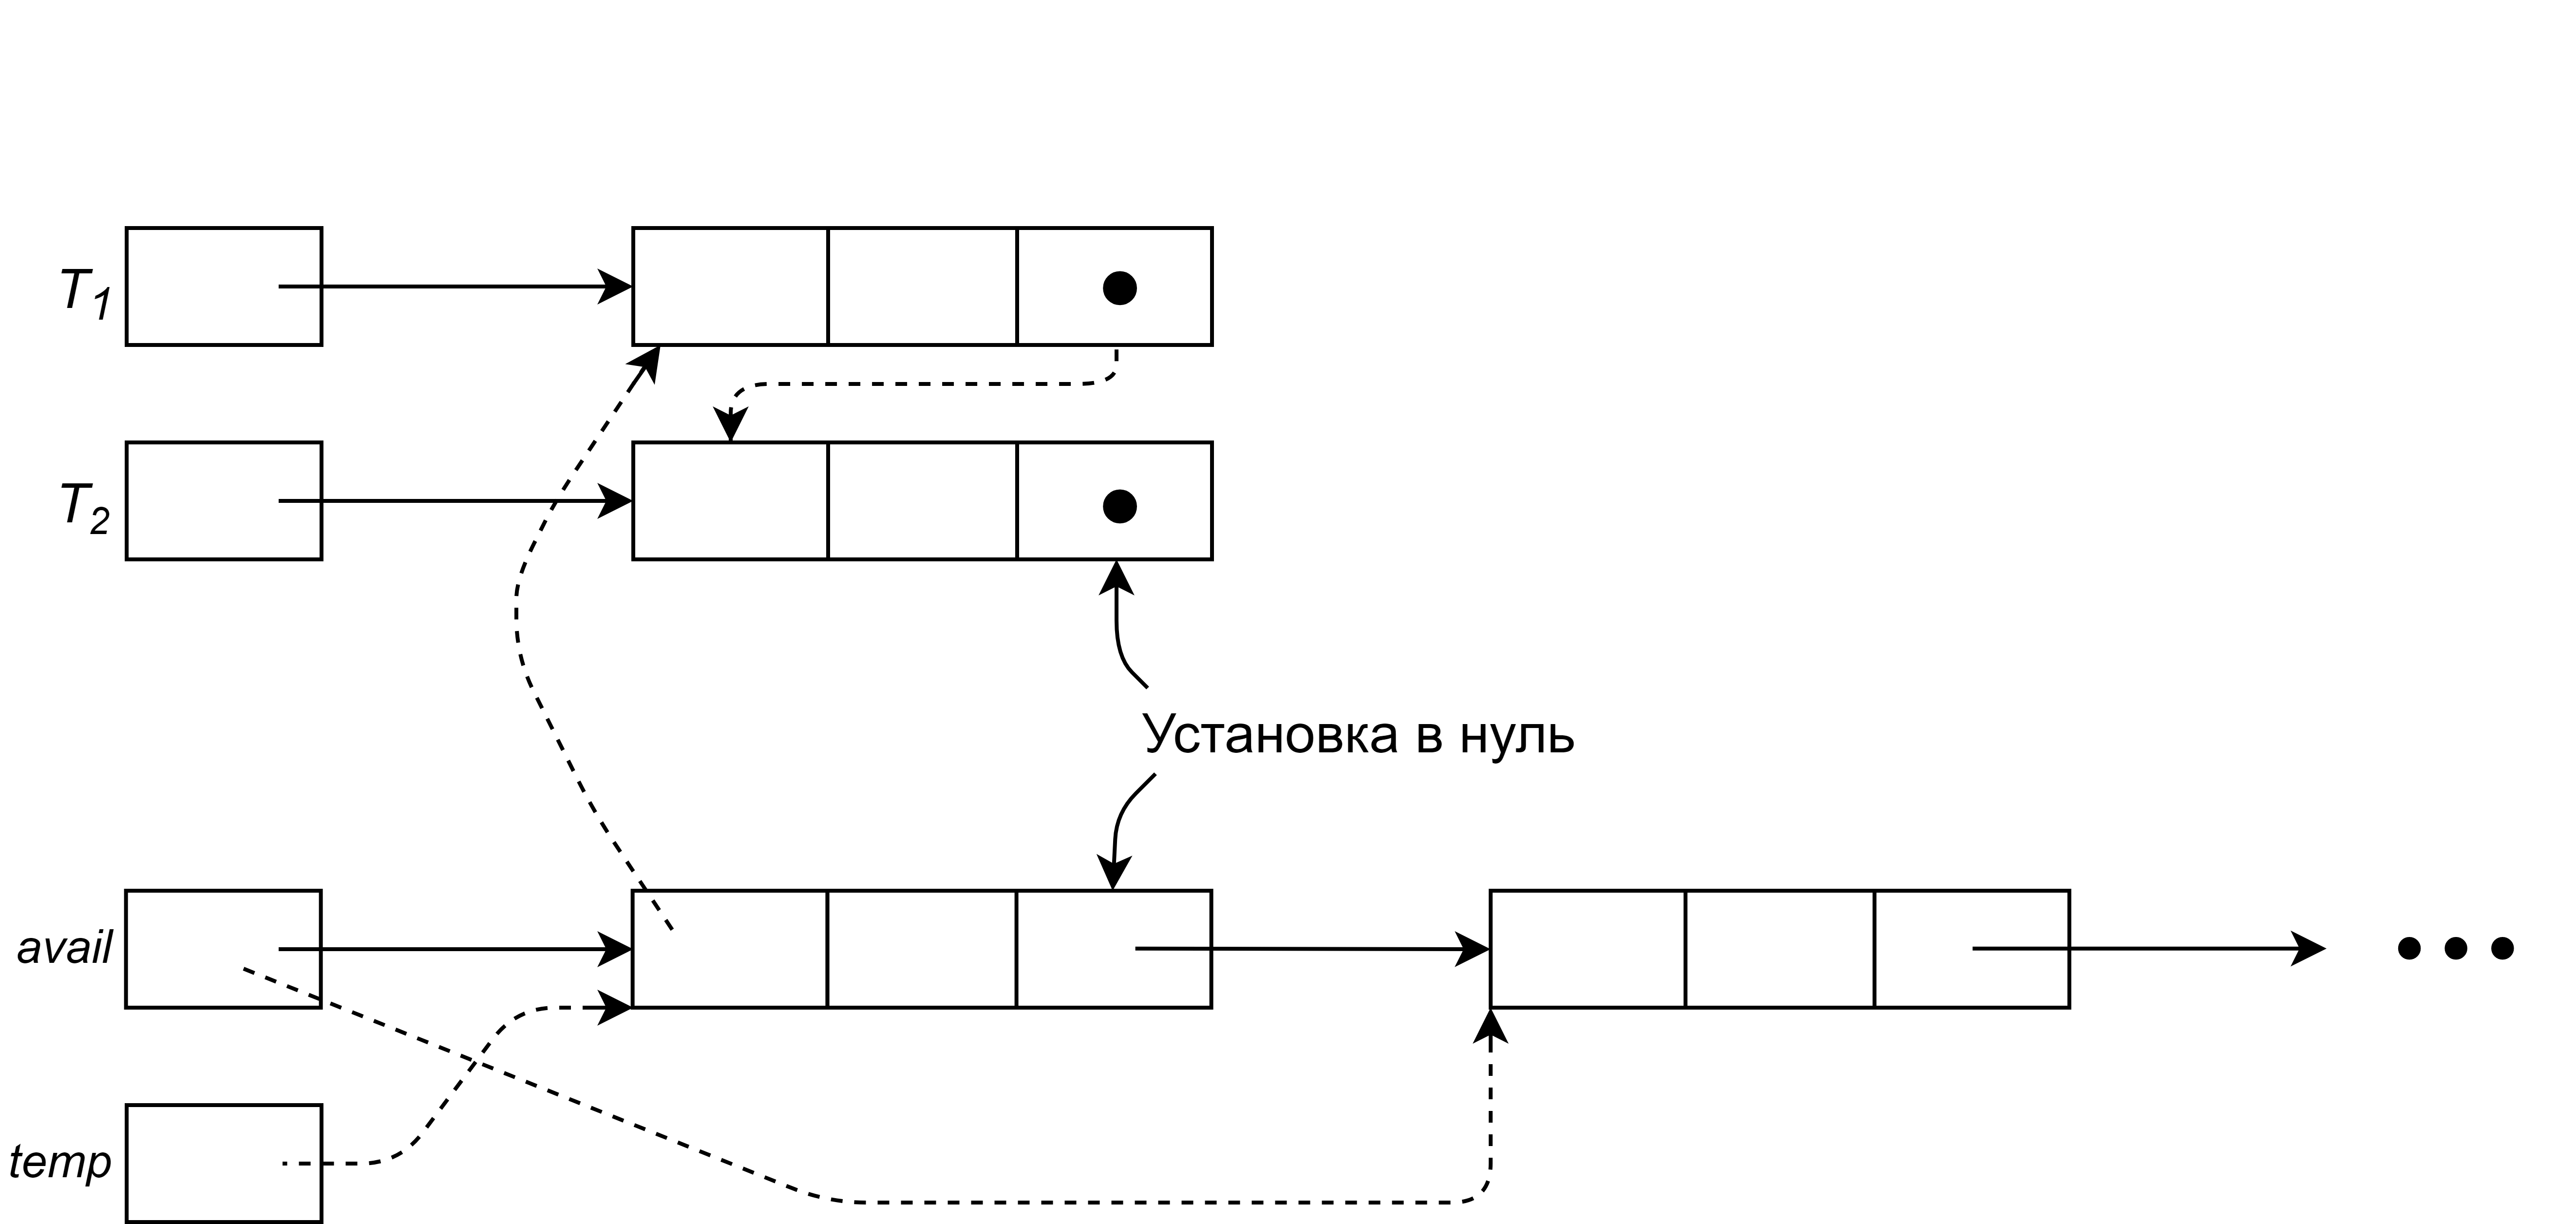
\includegraphics[scale=0.072]{pictures/p89}
\caption{ Изменение указателей при выполнении функции CREATE2}
\end{figure}

\indent Можно уменьшить область памяти, занимаемую узлами дерева (но при этом увеличится
время выполнения операторов), если в поле $right\_sibling$ самого правого сына
вместо нулевого указателя поместить указатель на родителя. Но в этом случае,
чтобы избежать двусмысленности, необходимо в каждую ячейку поместить еще двоичную
(логическую) переменную, которая будет показывать, что содержится в поле
$right\_sibling$: указатель на правого брата или указатель на родителя.

\indent При такой реализации можно найти для заданного узла его родителя, следуя за
указателями поля $right\_sibling$, пока не встретится указатель на родителя. В этом
случае время, необходимое для поиска родителя, пропорционально количеству сыновей
у родителя.

\section{Двоичные деревья}

\indent Деревья, которые мы определили в разделе 3.1, называются \textit{упорядоченными ориентированными
деревьями}, поскольку сыновья любого узла упорядочены слева направо,
а пути по дереву ориентированы от начального узла пути к его потомкам.
\textit{Двоичное} (или \textit{бинарное}) \textit{дерево} — совершенно другой вид.\rindex{Двоичное дерево}\rindex{Дерево!двоиное} Двоичное дерево может
быть или пустым деревом, или деревом, у которого любой узел или не имеет сыновей,
или имеет либо \textit{левого сына}, либо \textit{правого сына}, либо обоих. Тот факт, что каждый
сын любого узла определен как левый или как правый сын, существенно отличает
двоичное дерево от упорядоченного ориентированного дерева.

\indent \textbf{Пример 3.9}. Если мы примем соглашение, что на схемах двоичных деревьев левый
сын всегда соединяется с родителем линией, направленной влево и вниз от родителя,
а правый сын — линией, направленной вправо и вниз, тогда на рис. 3.12,а, б
представлены два различных дерева, хотя они оба похожи на обычное
(упорядоченное ориентированное) дерево, показанное на рис. 3.13. Пусть вас не смущает
тот факт, что деревья на рис. 3.12,а, б различны и не эквивалентны дереву на
рис. 3.13. Дело в том, что двоичные деревья нельзя непосредственно сопоставить
обычному дереву. Например, на рис. 3.12,а узел 2 является левым сыном узла 1 и
узел 1 не имеет правого сына, тогда как на рис. 3.12,6 узел 1 не имеет левого сына, а
имеет правого (узел 2). В тоже время в обоих двоичных деревьях узел 3 является левым
сыном узла 2, а узел 4 — правым сыном того же узла 2.$\square$

\indent Обход двоичных деревьев в прямом и обратном порядке в точности соответствует
таким же обходам обычных деревьев. При симметричном обходе двоичного дерева с корнем $n$ левым поддеревом $T_1$ и правым поддеревом $T_2$
сначала проходится поддерево
$T_1$, затем корень $n$ и далее поддерево $T_2$
. Например, симметричный обход дерева
на рис. 3.12,а даст последовательность узлов 3, 5, 2, 4, 1.

\begin{figure}[ht]
\begin{center}
\begin{minipage}[h]{0.4\linewidth}
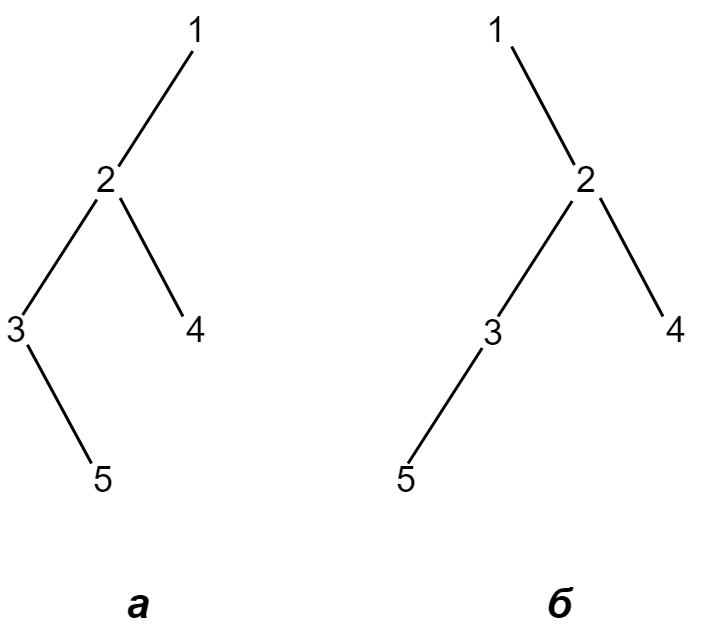
\includegraphics[width=1\linewidth, scale=0.8]{pictures/p90_1}
\caption{Два двоичных дерева.} %% подпись к рисунку
\end{minipage}
\hfill 
\begin{minipage}[h]{0.4\linewidth}
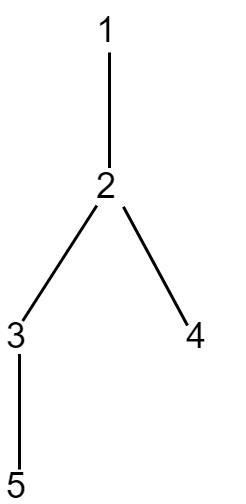
\includegraphics[scale=0.318]{pictures/p90_2}
\caption{"Обычное" дерево.}
\end{minipage}
\end{center}
\end{figure}

\subsection*{Представление двоичных деревьев}
\addcontentsline{toc}{subsection}{ Представление двоичных деревьев}
\rindex{Дерево!двоичное, представление}

\indent Если именами узлов двоичного дерева являются их номера 1, 2, ..., $n$, то подходящей
структурой для представления этого дерева может служить массив $cellspace$
записей с полями $leftchild$ (левый сын) и $rightchild$ (правый сын), объявленный следующим
образом:

\begin{lstlisting}[language=C, numbers=none]*
typedef /*соотв опис*/ record; 
typedef struct{ 
record cellspace[maxnodes];
int leftchild;
int rightchild;
}cellspace;
\end{lstlisting}

\indent В этом представлении $cellspace[i].leftchild$ является левым сыном узла $i$, a
$cellspace[i].rightchild$ — правым сыном. Значение 0 в обоих полях указывает на то,
что узел $i$ не имеет сыновей.

\indent \textbf{Пример 3.10}.  Двоичное дерево на рис. 3.12,а можно представить в виде табл. 3.1. $\square$

\begin{table}[ht]
\caption{\textbf{Представление двоичного дерева}}
\medskip
\begin{tabularx}{\textwidth}{ | X | X | }
\hline
Значение поля $leftchild$ & Значение поля $rightchild$\\ \hline
2 & 0 \\
3 & 4 \\
0 & 5 \\
0 & 0 \\
0 & 0 \\
\hline
\end{tabularx}
\label{table1}
\end{table}

\subsection*{Пример: коды Хаффмана\rindex{Коды Хаффмана}}
\addcontentsline{toc}{subsection}{ Пример: коды Хаффмана}

\indent Приведем пример применения двоичных деревьев в качестве структур данных.
Для этого рассмотрим задачу конструирования \textit{кодов Хаффмана}\rindex{Хаффмана коды}. Предположим, мы
имеем сообщения, состоящие из последовательности символов. В каждом сообщении
символы независимы и появляются с известной вероятностью, не зависящей от позиции
в сообщении. Например, мы имеем сообщения, состоящие из пяти символов $a$,
$b$, $c$, $d$, $e$, которые появляются в сообщениях с вероятностями 0.12, 0.4, 0.15, 0.08 и
0.25 соответственно.

\indent Мы хотим закодировать каждый символ последовательностью из нулей и единиц
так, чтобы код любого символа являлся префиксом кода сообщения, состоящего из
последующих символов. Это \textit{префиксное свойство} позволяет декодировать строку из
нулей и единиц последовательным удалением префиксов (т.е. кодов символов) из
этой строки.

\indent \textbf{Пример 3.11}.  В табл. 3.2 показаны две возможные кодировки для наших пяти
символов. Ясно, что первый код обладает префиксным свойством, поскольку любая
последовательность из трех битов будет префиксом для другой последовательности из
трех битов; другими словами, любая префиксная последовательность однозначно
идентифицируется символом. Алгоритм декодирования для этого кода очень прост:
надо поочередно брать по три бита и преобразовать каждую группу битов в соответствующие
символы. Например, последовательность 001010011 соответствует исходному сообщению bcd.

\begin{table}[ht]
\caption{\textbf{Два двоичных кода}}
\medskip
\begin{tabularx}{\textwidth}{  X | X | X | X  }
Символ & Вероятность & Код 1 & Код 2\\ \hline
a & 0.12 & 000 & 000 \\
b & 0.40 & 001 & 11 \\
c & 0.15 & 010 & 01 \\
d & 0.08 & 011 & 001 \\
e & 0.25 & 100 & 10 \\
\end{tabularx}
\label{table2}
\end{table}

\indent Легко проверить, что второй код также обладает префиксным свойством. Процесс
декодирования здесь не отличается от аналогичного процесса для первого кода. Единственная
сложность для второго кода заключается в том, что нельзя сразу всю последовательность
битов разбить на отдельные сегменты, соответствующие символам, так как
символы могут кодироваться и двумя и тремя битами. Для примера рассмотрим двоичную
последовательность 1101001, которая опять представляет символы $bcd$. Первые
два бита 11 однозначно соответствуют символу $b$, поэтому их можно удалить, тогда получится
01001. Здесь 01 также однозначно определяет символ $c$ и т.д.$\square$

\indent Задача конструирования кодов Хаффмана\rindex{Задача!конструирования кодов Хаффмана} заключается в следующем: имея множество
символов и значения вероятностей их появления в сообщениях, построить
такой код с префиксным свойством, чтобы средняя длина кода (в вероятностном
смысле) последовательности символов была минимальной. Мы хотим минимизировать
среднюю длину кода для того, чтобы уменьшить длину вероятного сообщения
(т.е. чтобы сжать сообщение). Чем короче среднее значение длины кода символов,
тем короче закодированное сообщение. В частности, первый код из примера 3.11
имеет среднюю длину кода 3. Это число получается в результате умножения длины
кода каждого символа на вероятность появления этого символа. Второй код имеет
среднюю длину 2.2, поскольку символы $a$ и $d$ имеют суммарную вероятность появления
0.20 и длина их кода составляет три бита, тогда как другие символы имеют код
длиной 2\footnote[1]{ Отсюда следует очевидный вывод, что символы с большими вероятностями появления
должны иметь самые короткие коды. — \textit{Прим. ред.}}.

\indent Можно ли придумать код, который был бы лучше второго кода? Ответ положительный:
существует код с префиксным свойством, средняя длина которого равна 2.15. Это
наилучший возможный код с теми же вероятностями появления символов. Способ
нахождения оптимального префиксного кода называется \textit{алгоритмом Хаффмана}. \rindex{Алгоритм!Хаффмана} В
этом алгоритме находятся два символа $a$ и $b$ с наименьшими вероятностями появления
и заменяются одним фиктивным символом, например $x$, который имеет вероятность
появления, равную сумме вероятностей появления символов $a$ и $b$. Затем, используя
эту процедуру рекурсивно, находим оптимальный префиксный код для меньшего множества символов (где символы $a$ и $b$ заменены одним символом $x$). Код
для исходного множества символов получается из кодов замещающих символов путем
добавления 0 и 1 перед кодом замещающего символа, и эти два новых кода принимаются
как коды заменяемых символов. Например, код символа $a$ будет соответствовать
коду символа $x$ с добавленным нулем перед этим кодом, а для кода символа $b$ перед кодом символа $x$ будет добавлена единица.

\indent Можно рассматривать префиксные коды как пути на двоичном дереве: прохождение
от узла к его левому сыну соответствует 0 в коде, а к правому сыну — 1. Если
мы пометим листья дерева кодируемыми символами, то получим представление префиксного
кода в виде двоичного дерева. Префиксное свойство гарантирует, что нет
символов, которые были бы метками внутренних узлов дерева (не листьев), и наоборот,
помечая кодируемыми символами только листья дерева, мы обеспечиваем префиксное
свойство кода этих символов.

\indent \textbf{Пример 3.12}.  Двоичные деревья для кодов 1 и 2 из табл. 3.2 показаны на рис. 3.14
(дерево слева соответствует коду 1, а дерево справа — коду 2).$\square$

\begin{figure}[ht]
\centering
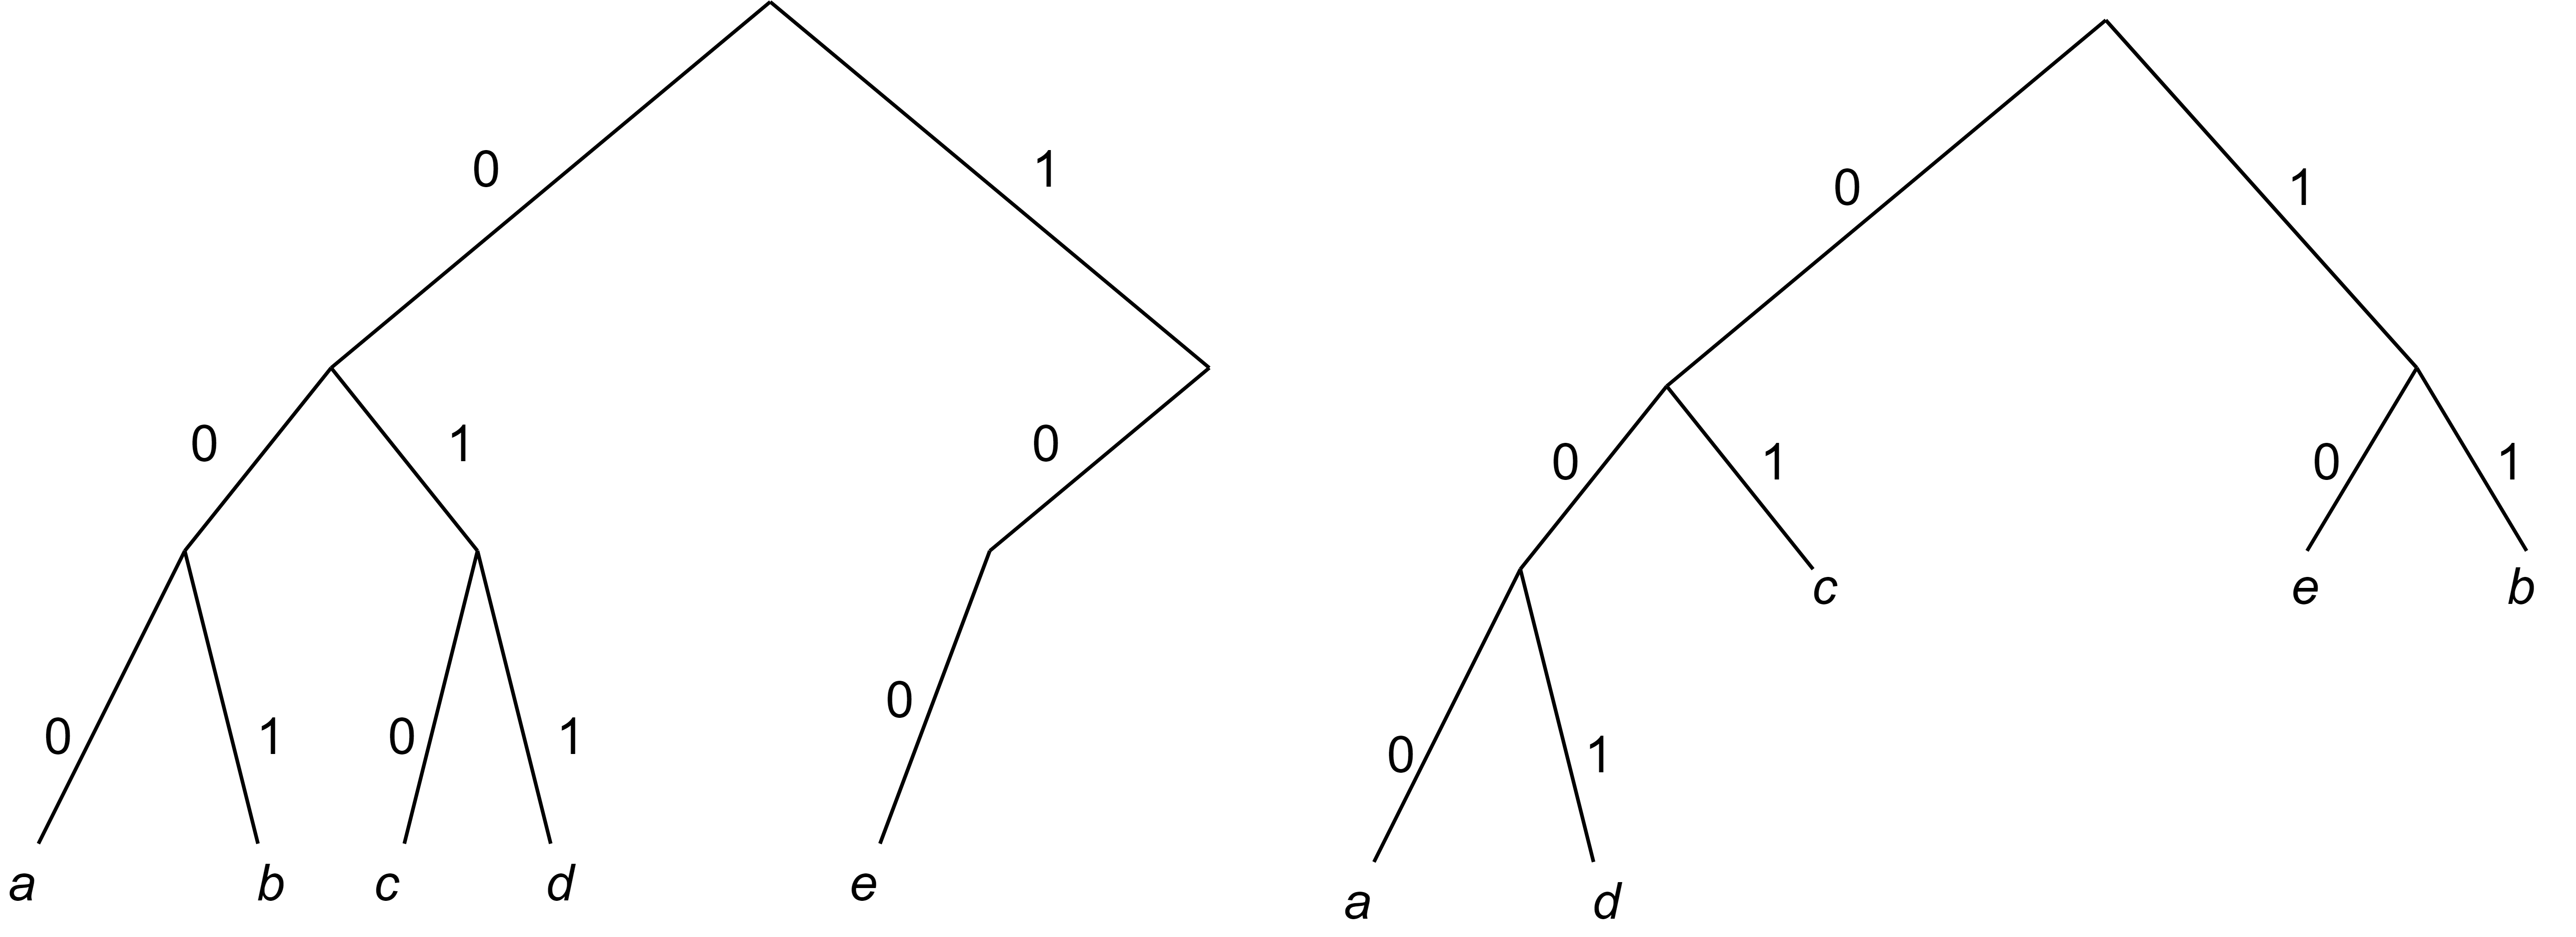
\includegraphics[scale=0.075]{pictures/p92}
\caption{ Двоичные деревья, представляющие коды с префиксным свойством}
\end{figure}

\indent Для реализации алгоритма Хаффмана мы используем лес, т.е. совокупность деревьев,
чьи листья будут помечены символами, для которых разрабатывается кодировка,
а корни помечены суммой вероятностей всех символов, соответствующих листьям
дерева. Мы будем называть эти суммарные вероятности \rindex{Вес дерева} \rindex{Дерево!вес} весом дерева. Вначале
каждому символу соответствует дерево, состоящее из одного узла, в конце работы алгоритма
мы получим одно дерево, все листья которого будут помечены кодируемыми
символами. В этом дереве путь от корня к любому листу представляет код для символа-метки
этого листа, составленный по схеме, согласно которой левый сын узла соответствует
0, а правый — 1 (как на рис. 3.14).

\indent Важным этапом в работе алгоритма является выбор из леса двух деревьев с наименьшими
весами. Эти два дерева комбинируются в одно с весом, равным сумме весов
составляющих деревьев. При слиянии деревьев создается новый узел, который
становится корнем объединенного дерева и который имеет в качестве левого и правого
сыновей корни старых деревьев. Этот процесс продолжается до тех пор, пока не
получится только одно дерево. Это дерево соответствует коду, который при заданных
вероятностях имеет минимально возможную среднюю длину.

\indent \textbf{Пример 3.13}.  Последовательные шаги выполнения алгоритма Хаффмана для кодируемых
символов и их вероятностей, заданных в табл. 3.2, представлены на
рис. 3.15. Здесь видно (рис. 3.15,д), что символы $a, b, c, d$ и $e$ получили соответственно
коды 1111, 0, 110, 1110 и 10. В этом примере существует только одно нетривиальное
дерево, соответствующее оптимальному коду, но в общем случае их может
быть несколько. Например, если бы символы Ь и е имели вероятности соответственно
0.33 и 0.32, то после шага алгоритма, показанного на рис. 3.15,в, можно было бы
комбинировать $b$ и $e$, а не присоединять $e$ к большому дереву, как это сделано на
рис. 3.15,г$\square$

\begin{figure}[ht]
\centering
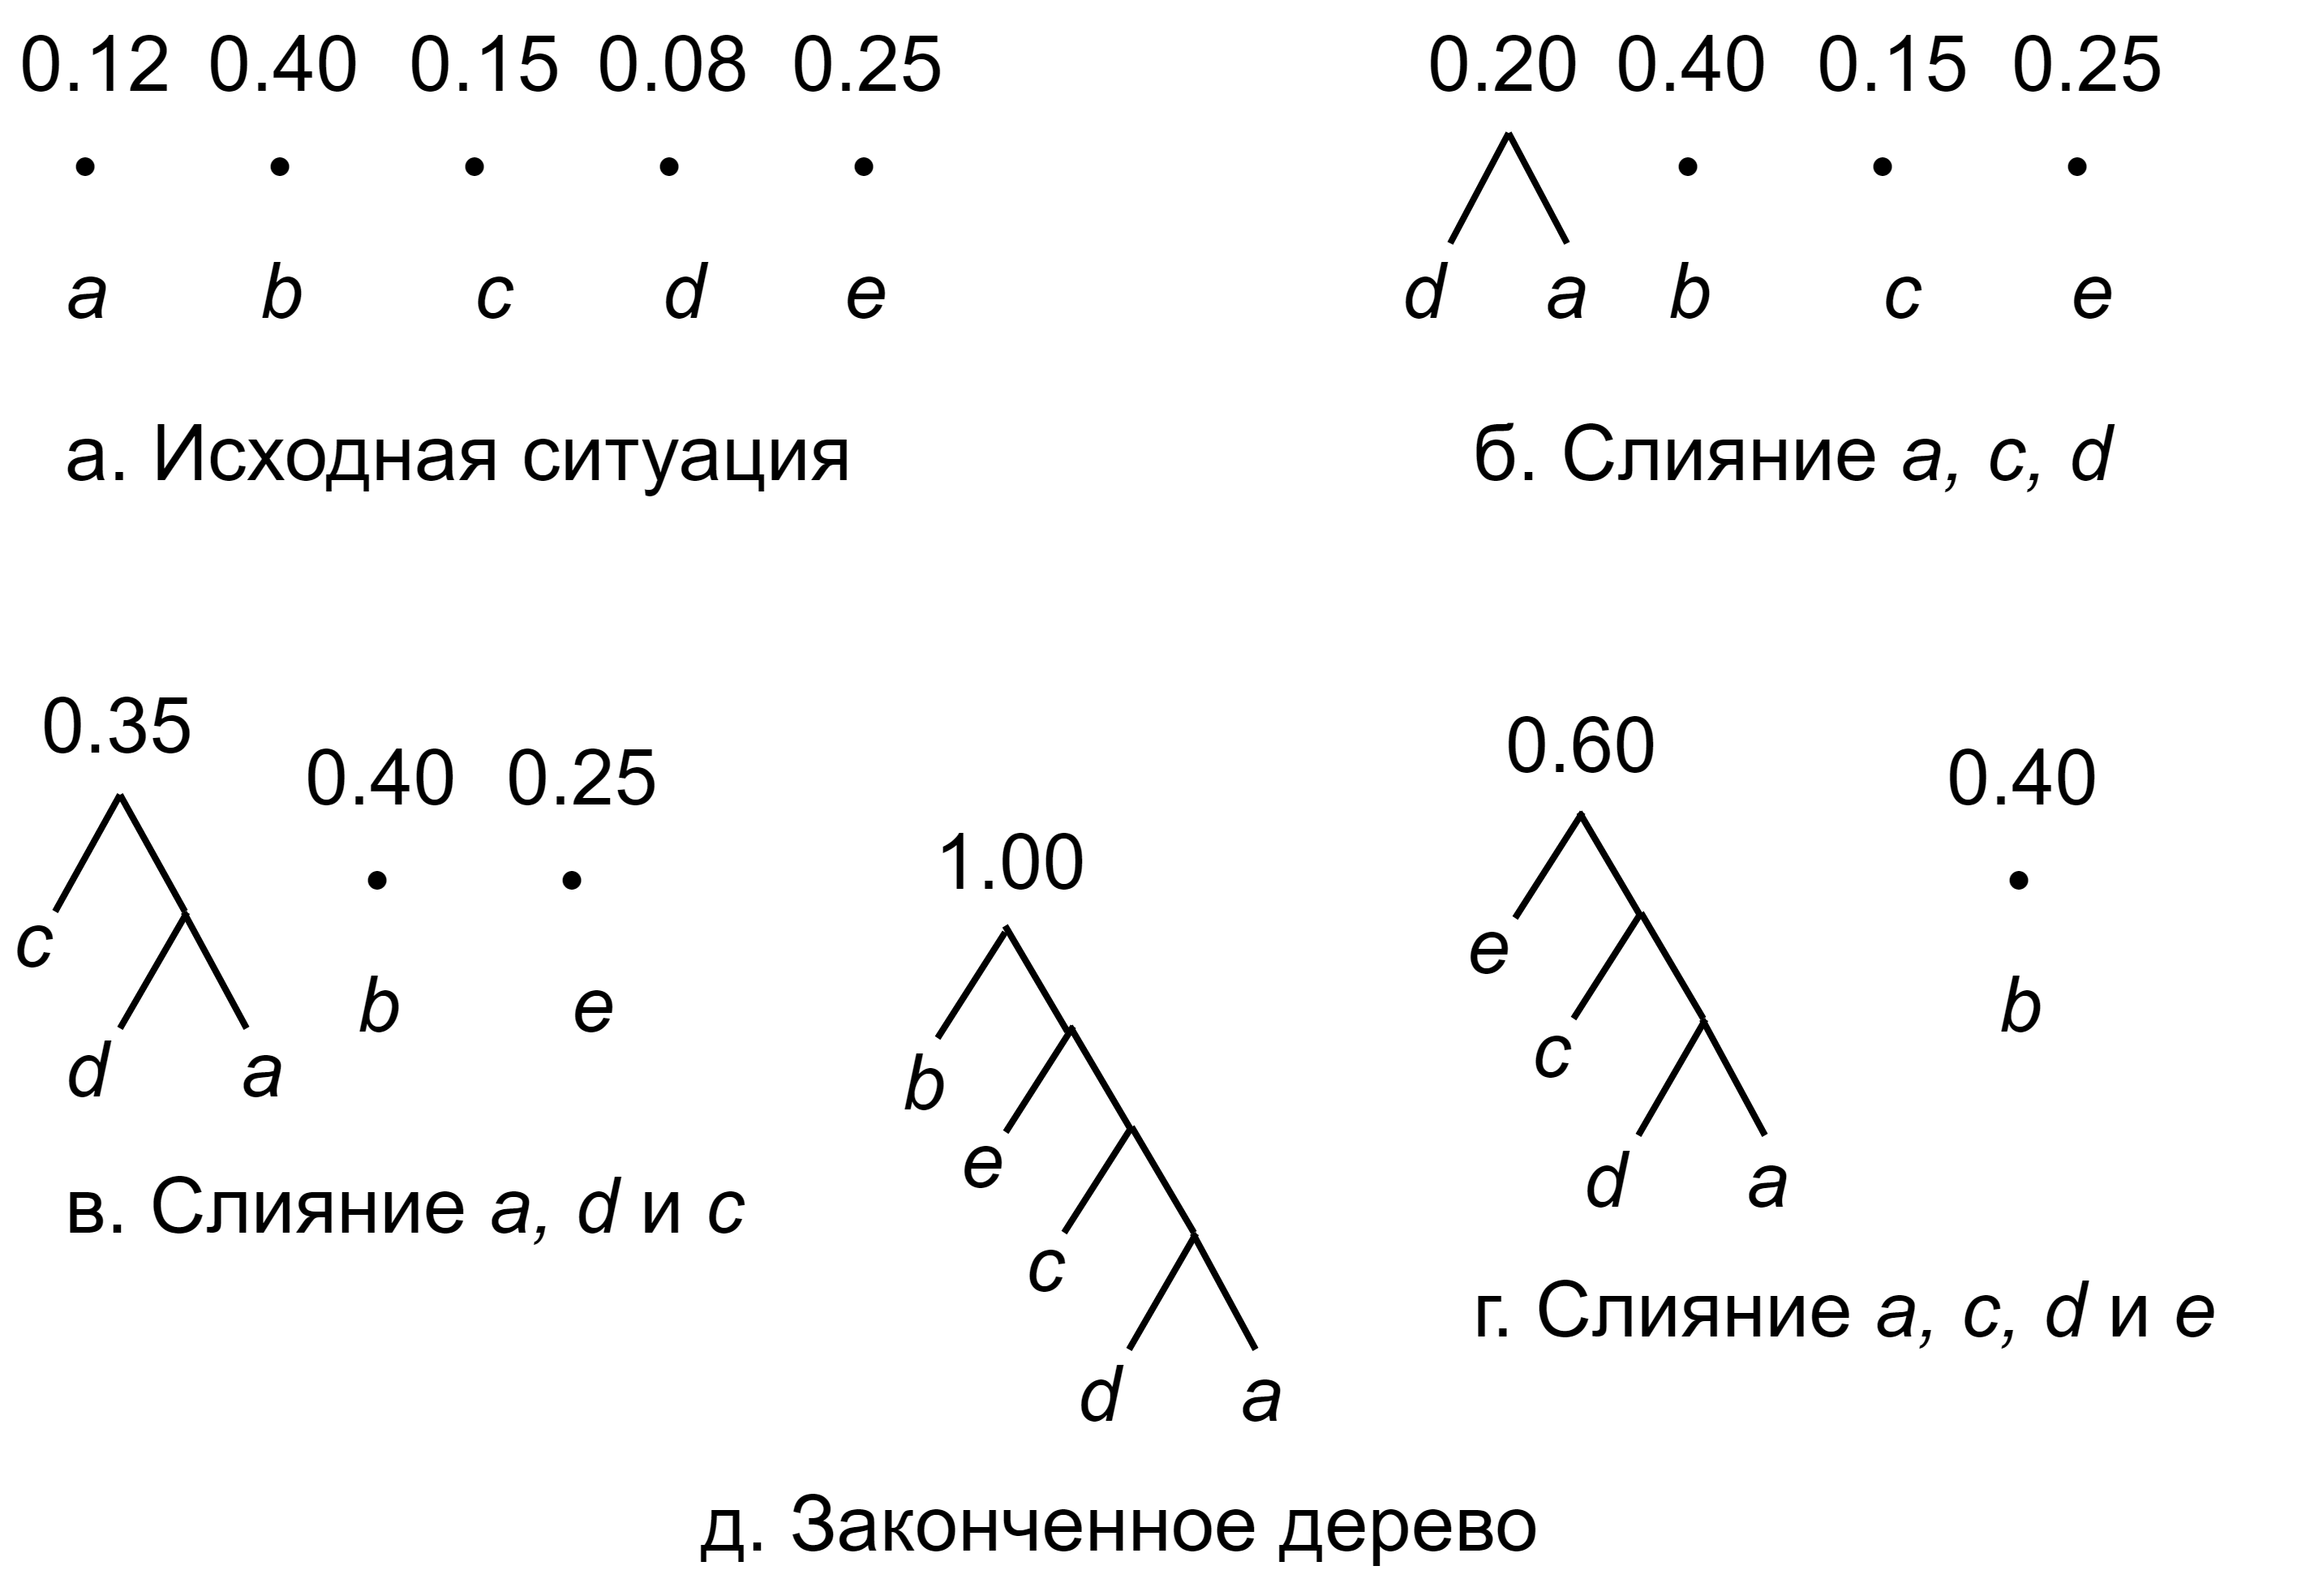
\includegraphics[scale=0.1]{pictures/p93}
\caption{ Этапы создания дерева Хаффмана}
\end{figure}

\indent Теперь опишем необходимые структуры данных. Во-первых, для представления
двоичных деревьев мы будем использовать массив TREE (Дерево), состоящий из записей
следующего типа:

\newpage

\begin{lstlisting}[language=C, numbers=none]*
typedef struct{ 
int parent;
int leftchild;
int rightchild;
}Tree;
\end{lstlisting}



Указатели в поле $parent$ (родитель) облегчают поиск путей от листа к корню при записи
кода символов. Во-вторых, мы используем массив ALPHABET (Алфавит), также
состоящий из записей, которые имеют следующий тип:

\begin{lstlisting}[language=C, keepspaces = true, numbers=none]*
typedef struct{ 
char symbol;
float probability;
int leaf; // курсор
}ALPHABET;
\end{lstlisting}


В этом массиве каждому символу (поле $symbol$), подлежащему кодированию, ставится
в соответствие вероятность его появления (поле $probability$) и лист, меткой которого
он является (поле $leaf$). В-третьих, для представления непосредственно деревьев
необходим массив FOREST (Лес). Этот массив будет состоять из записей с полями
$weight$ (вес) и $root$ (корень) следующего типа:

\begin{lstlisting}[language=C, numbers=none]*
typedef struct{ 
float weight;
int root;
}FOREST;
\end{lstlisting}

\indent Начальные значения всех трех массивов, соответствующих данным на рис. 3.15,а,
показаны на рис. 3.16. Эскиз программы (псевдопрограмма, т.е. программа на
псевдоязыке, как описано в главе 1) построения дерева Хаффмана представлен в
листинге 3.8.

\begin{figure}[ht]
\centering
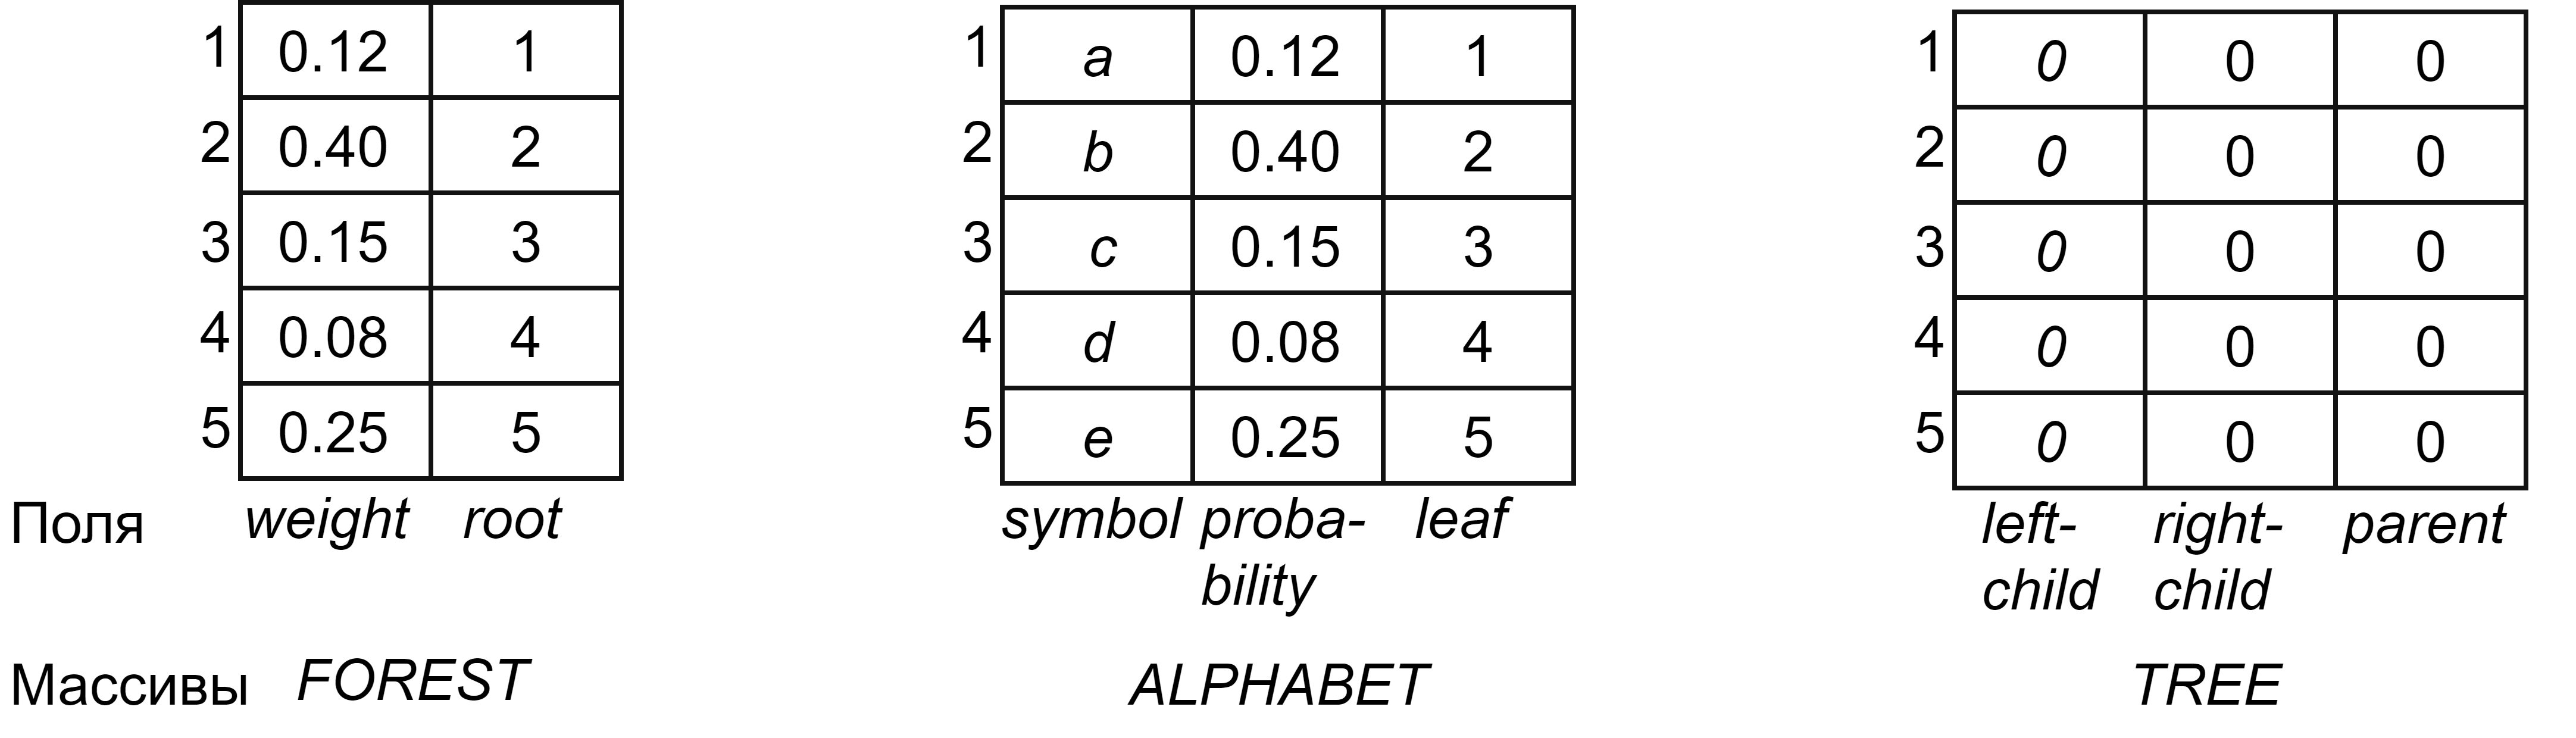
\includegraphics[scale=0.1]{pictures/p94}
\caption{ Исходное состояние массивов}
\end{figure}

\begin{lstlisting}[language=C, captionpos=t, keepspaces = true, caption = {Программа построения дерева Хаффмана}]
    while (существует более одного дерева в лесу){
        i = индекс дерева в FOREST  
                        c наименьшим весом;
        j = индекс дерева в FOREST 
                        со вторым наименьшим весом;
        Создание нового узла с левым сыном FOREST[i].root 
                        и правым сыном FOREST[j].root;
        Замена в FOREST дерева i деревом, 
                чьим корнем является новый узел и 
                чей вес равен 
                FOREST[i].weight + FOREST[j].weight;
        Удаление дерева j из массива FOREST;
    }
\end{lstlisting}

\indentДля реализации строки (4) листинга 3.8, где увеличивается количество используемых
ячеек массива TREE, и строк (5) и (6), где уменьшается количество ячеек
массива FOREST, мы будем использовать курсоры $lasttree$ (последнее дерево) и
$lastnode$ (последний узел), указывающие соответственно на массив FOREST и массив
TREE. Предполагается, что эти курсоры располагаются в первых ячейках соответствующих
массивов\footnote[1]{  Для этапа чтения данных, который мы опускаем, необходим также курсор для массива
ALPHABET, который бы "следил"\ за заполнением данными этого массива.}. Мы также предполагаем, что все массивы имеют определенную
объявленную длину, но здесь мы не будем проводить сравнение этих ограничивающих
значений со значениями курсоров.

\indent В листинге 3.9 приведены коды двух полезных процедур. Первая из них,
$lightones$, выполняет реализацию строк (2) и (3) листинга 3.8 по выбору индексов
двух деревьев с наименьшими весами. Вторая процедура, функция $create(n_1, n_2)$\rindex{Программа!create}
создает новый узел и делает заданные узлы $n_1$ и $n_2$ левым и правым сыновьями
этого узла.

\begin{lstlisting}[language=C, captionpos=t, numbers=none, caption = { Две процедуры}]
    void lightones(int least, int second){
        /*
        |Присваивает переменным least и second индексы массива |
        |FOREST, соответствующие деревьям с наименьшими весами.|
        |Предполагается, что lasttree > 2|
        */
        int i;
        // |Рассматриваются первые два дерева|
        if(FOREST[l].weight <= FOREST[2].weight){
            least = 1;
            second = 2;
        }
        else{
            least = 2;
            second = 1;
        }
        for(i = 3; i = lasttree; i++){
            if(FOREST[i].weight < FOREST[least].weight){
                second = least;
                least = i;
            }
            else{
                if(FOREST[i].weight < FOREST[second].weight)
                    second = i;
            }
        }
    }


    int create(int lefttree, righttree){
        /*
        |Возвращает новый узел, у которого левым и правым сыновьями|
        |становятся FOREST[lefttree].root и FOREST[righttree].root |
        */
        lastnode:= lastnode + 1; //| ячейка TREE[lastnode] для нового узла|
        Tree[lastnode].leftchild = FOREST[lefttree].root;
        TREE[lastnode].rightchild = FOREST[righttree].root; //| теперь введем указатели для нового узла и его сыновей |
        TREE[lastnode].parent = 0;
        TREE[FOREST[lefttree].root].parent = lastnode;
        TREE[FOREST[righttree].root].parent = lastnode;
        return lastnode;
    } 
\end{lstlisting}

\indent Теперь все неформальные операторы листинга 3.8 можно описать подробнее. В
листинге 3.10 приведен код процедуры Huffman\rindex{Программа!Huffman}, которая не осуществляет ввод и
вывод, а работает со структурами, показанными на рис. 3.16, которые объявлены
как глобальные.

\begin{lstlisting}[language=C, captionpos=t, keepspaces = true, numbers=none, caption = { Реализация алгоритма Хаффмана}]
    void Huffman(int i, int j){
    // i,j - два дерева с наименьшими весами из FOREST
        int newroot;
        while(lasttree > 1){
            lightones(i, j);
            newroot = create(i, j); //  далее дерево i заменяется деревом с корнем newroot 
            FOREST[i].weight = FOREST[i].weight + FOREST[j].weight;
            FOREST[i].root = newroot; //  далее дерево j заменяется на дерево lasttree,
            //  массив FOREST уменьшается на одну запись 
        }
    } 
\end{lstlisting}

\indent На рис. 3.17 показана структура данных из рис. 3.16 после того, как значение
переменной $lasttree$ уменьшено до 3, т.е. лес имеет вид, показанный на рис. 3.15,в.

\begin{figure}[ht]
\centering
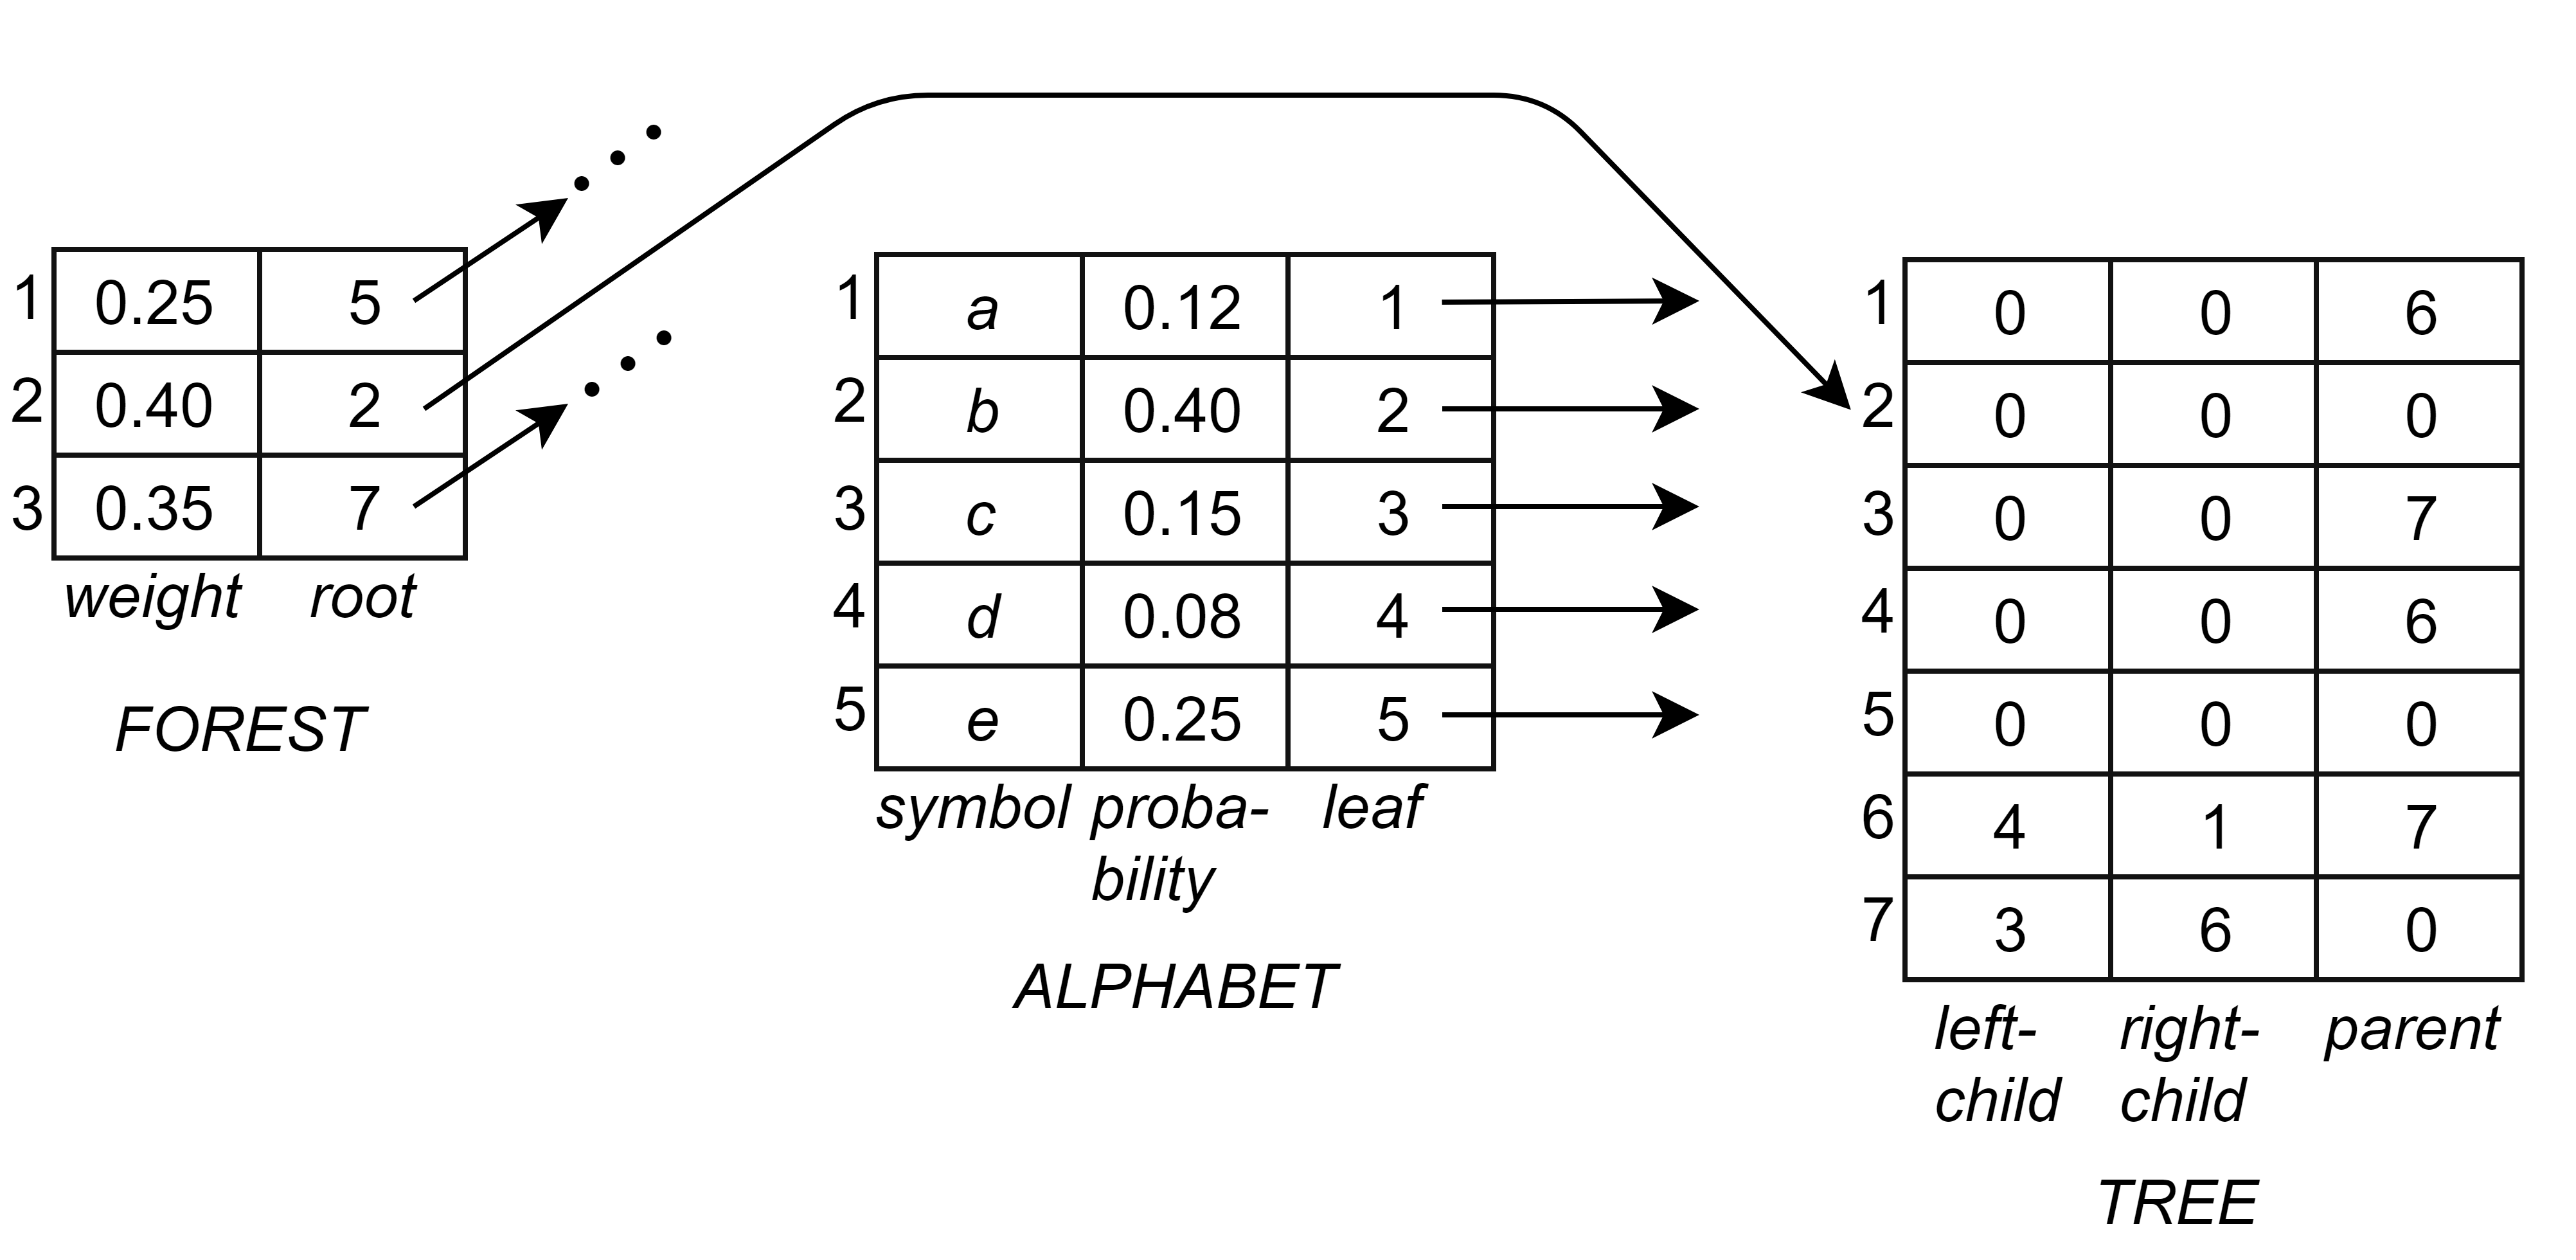
\includegraphics[scale=0.08]{pictures/p96}
\caption{ Структура данных после двух итераций}
\end{figure}

\indent После завершения работы алгоритма код каждого символа можно определить следующим
образом. Найдем в массиве ALPHABET запись с нужным символ в поле
$symbol$. Затем по значению поля $leaf$ этой же записи определим местоположение записи
в массиве TREE, которая соответствует листу, помеченному рассматриваемым
символом. Далее последовательно переходим по указателю parent от текущей записи,
например соответствующей узлу п, к записи в массиве TREE, соответствующей его
родителю $p$. По родителю $p$ определяем, в каком его поле, $leftchild$ или $rightchild$,
находится указатель на узел $n$, т.е. является ли узел $n$ левым или правым сыном, и в
соответствии с этим печатаем 0 (для левого сына) или 1 (для правого сына). Затем
переходим к родителю узла $p$ и определяем, является ли его сын $p$ правым или левым,
и в соответствии с эти печатаем следующую 1 или 0, и т. д. до самого корня
дерева. Таким образом, код символа будет напечатан в виде последовательности битов,
но в обратном порядке. Чтобы распечатать эту последовательность в прямом порядке,
надо каждый очередной бит помещать в стек, а затем распечатать содержимое
стека в обычном порядке.

\subsection*{Реализация двоичных деревьев с помощью указателей}\rindex{Реализация!двоичных деревьев с помощью указателей}\rindex{Дерево!двоичное, реализация}
\addcontentsline{toc}{subsection}{ Реализация двоичных деревьев с помощью указателей}

\indent Для указания на правых и левых сыновей (и родителей, если необходимо) вместо
курсоров можно использовать настоящие указатели языка Си. Например, можно
сделать объявление

\begin{lstlisting}[language=C, numbers=none]*
    typedef struct{ 
        int value;
        |\textbf{Tree}|* leftchild;
        |\textbf{Tree}|* rightchild;
    }Tree;
\end{lstlisting}
				


Используя этот тип данных узлов двоичного дерева, функцию \textit{create} (листинг 3.9) можно переписать так, как показано в следующем листинге.
\begin{lstlisting}[language=C, caption={Код функции \textit{create} при реализации двоичного дерева с помощью указателей}, numbers = none]
    node *create(node *lefttree, *righttree) {
        |\textbf{node}| *root;
        new_node(&root);
        root->leftchild   = lefttree;
        root->rightchild  = righttree;
        root->parent      = 0;
        lefttree->parent  = root;
        righttree->parent = root;
        return root; /* create */
    }
\end{lstlisting}


\subsection*{Упражнения}
\addcontentsline{toc}{subsection}{ Упражнения}

\begin{itemize}
	\item[3.1]Ответьте на следующие вопросы о дереве, показанном на рис. 3.18:
	
	\begin{itemize}
		\item[а)] какие узлы этого дерева я вляются листьями?
		\item[б)] какой узел является корнем дерева?
		\item[в)] какой узел является родителем узла С?
		\item[г)] назовите сыновей узла С;
		\item[д)] назовите предков узла Е;
		\item[е)] назовите потомков узла Е;
		\item[ж)] какие узлы являются правыми братьями узлов D и E?
		\item[з)] какие узлы лежат слева и справа от узла G?
		\item[и)] какова глубина узла С?
		\item[к)] какова высота узла С?
	\end{itemize}
	\begin{figure}[ht!]
		\center{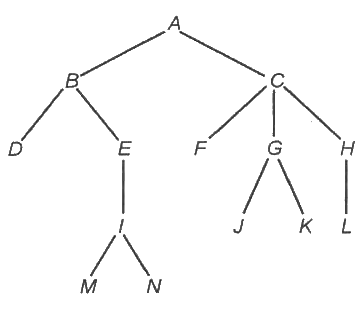
\includegraphics[scale=0.6] {3,18.png}}
		\caption{\textit{Дерево}} 
	\end{figure}

	\item[3.2]Сколько путей длины 3 существует на дереве, показанном на рис. 3.18?
	\item[3.3]Напишите программы вычисления высоты дерева с использованием трех представлений деревьев, описанных в разделе 3.3.
	
	\fancyfoot[LO]{УПРАЖНЕНИЯ}

	
	\item[3.4]Составьте списки узлов дерева, представленного на рис. 3.18, при обходе этого дерева
	\begin{itemize}
		\item[а)] в прямом порядке;
		\item[б)] в обратном порядке;
		\item[в)] во внутреннем порядке;
	\end{itemize}
	\item[3.5]Пусть два различных узла \textit{m} и \textit{n} принадлежат одному и тому же дереву. Покажите, что только одно из следующих утверждений может быть истинным:
	\begin{itemize}
		\item[а)]узел \textit{m} расположен слева от узла \textit{n};
		\item[б)]узел \textit{m} расположен справа от узла \textit{n};
		\item[в)]узел \textit{m} - истинный предок узла \textit{n};
		\item[г)]узел \textit{m} - истинный потомок узла \textit{n};
	\end{itemize}
	\item[3.6]Поставьте галочку в ячейку на пересечении строки \textit{i} и столбца \textit{j}, если одновременно выполняются условия, представленные в заголовках строки \textit{i} и столбца $j$.
	%%%%%%непонятная табличка на стр 100%%%%%%%%% %%%%%%%%%%%%

\begin{onehalfspace}
	\small
	\begin{table}[ht]
		\begin{center}
			\begin{tabular}{lccc}
				& Узел $n$ предшествует &  Узел $n$ предшествует & Узел $n$ предшествует \\
				& узлу $m$ при обходе      & узлу $m$ при обходе       & узлу $m$ при \\	 
				& дерева в прямом	       & дерева в обратном	     & симметричном \\
				& порядке			       & порядке			     & обходе \\
				\\[-1em] \cline{2-4} 
				& \multicolumn{1}{|c|}{}  & \multicolumn{1}{c|}{}  & \multicolumn{1}{c|}{} \\[-0.8em]
				Узел $n$		& \multicolumn{1}{|c|}{}  & \multicolumn{1}{c|}{}  & \multicolumn{1}{c|}{} \\
				расположен	& \multicolumn{1}{|c|}{}  & \multicolumn{1}{c|}{}  & \multicolumn{1}{c|}{} \\
				слева от 		& \multicolumn{1}{|c|}{}  & \multicolumn{1}{c|}{}  & \multicolumn{1}{c|}{} \\
				узла $m$ 	& \multicolumn{1}{|c|}{}  & \multicolumn{1}{c|}{}  & \multicolumn{1}{c|}{} \\ \cline{2-4}	
				Узел $n$		& \multicolumn{1}{|c|}{}  & \multicolumn{1}{c|}{}  & \multicolumn{1}{c|}{} \\
				расположен	& \multicolumn{1}{|c|}{}  & \multicolumn{1}{c|}{}  & \multicolumn{1}{c|}{} \\
				справа от 	& \multicolumn{1}{|c|}{}  & \multicolumn{1}{c|}{}  & \multicolumn{1}{c|}{} \\
				узла $m$		& \multicolumn{1}{|c|}{}  & \multicolumn{1}{c|}{}  & \multicolumn{1}{c|}{} \\ \cline{2-4}
				Узел $n$ - 	& \multicolumn{1}{|c|}{}  & \multicolumn{1}{c|}{}  & \multicolumn{1}{c|}{} \\
				истинный	& \multicolumn{1}{|c|}{}  & \multicolumn{1}{c|}{}  & \multicolumn{1}{c|}{} \\
				предок		& \multicolumn{1}{|c|}{}  & \multicolumn{1}{c|}{}  & \multicolumn{1}{c|}{} \\
				узла $m$ 	& \multicolumn{1}{|c|}{}  & \multicolumn{1}{c|}{}  & \multicolumn{1}{c|}{} \\ \cline{2-4}	
				Узел $n$ - 	& \multicolumn{1}{|c|}{}  & \multicolumn{1}{c|}{}  & \multicolumn{1}{c|}{} \\
				истинный	& \multicolumn{1}{|c|}{}  & \multicolumn{1}{c|}{}  & \multicolumn{1}{c|}{} \\
				потомок 	& \multicolumn{1}{|c|}{}  & \multicolumn{1}{c|}{}  & \multicolumn{1}{c|}{} \\
				узла $m$ 	& \multicolumn{1}{|c|}{}  & \multicolumn{1}{c|}{}  & \multicolumn{1}{c|}{} \\ \cline{2-4}		
				\\[-0.8em]
			\end{tabular}
		\end{center}
	\end{table}
\end{onehalfspace}	
	
	Например поставьте галочку в ячейку на пересечение третьей строки и второго столбца, если уверены, что узел\textit{n} может быть истинным предком узла \textit{m} 
	и в тоже время предшествовать узлу \textit{m} при обходе дерева в обратном порядке.
	\item[3.7]Предположим, что массивы PREORDER[\textit{n}], INORDER[\textit{n}] и POSTORDER[\textit{n}], содержащие списки узлов дерева, полученные при его обходе в прямом, внутреннем и обратном порядке
	соотвотственно. Используя эти массивы, опишите алгоритм, который для любой пары узлов \textit{i} и \textit{j} определяет, является ли узел \textit{i} предком узла \textit{j}.
	\item[*3.8]Существует способ проверить, является ли один узел истинным предком другого узла, который основан на следующем правиле: узел \textit{m} является истинным предком узла \textit{n}, если узел \textit{m}
	предшествует узлу \textit{n} при обходе дерева в X порядке, но следует за узлом \textit{n} при обходе в Y порядке, где X и Y выбираются из множества \{\textit{прямом, обратном, внутреннем}\}. Определите все возможные пары X и Y,
	когда это правило справедливо.
	\item[3.9]Напишите программы обхода двоичных деревьев
	\begin{itemize}
		\item[а)]в прямом порядке;
		\item[б)]в обратном порядке;
		\item[в)]во внутреннем порядке.
	\end{itemize}
	
	\fancyfoot[RE]{ГЛАВА 3. ДЕРЕВЬЯ}

	
	\item[3.10]При прохождении дерева \textit{в порядке уровней} \rindex{Обход дерева!в порядке уровней}в список узлов сначала заносится корень дерева, затем все узлы глубины 1, далее все узлы глубины 2 и т.д.
	Узлы одной глубины заносятся в список узлов в порядке слева направо. Напишите программу обхода деревьев в порядке уровней.
	\item[3.11]Преобразуйте выражение $((a+b)+c*(d+e)+f)*(g+h)$
	\begin{itemize}
		\item[а)]в префиксную форму;
		\item[б)]в постфиксную форму.
	\end{itemize}
	\item[3.12]Нарисуйте дерево, соответствующее префиксным выражениям
	\begin{itemize}
		\item[а)]$*a+b*c+de$;
		\item[б)]$*a+*b+cde$.
	\end{itemize}
	\item[3.13]Пусть дерево \textit{Т} - дерево, в котором каждый узел, не являющийся листом, имеет ровно двух сыновей. Напишите программы преобразования
	\begin{itemize}
		\item[а)]списка узлов дерева \textit{Т}, составленного при обходе дерева в прямом порядке, в список, составленный при обходе в обратном порядке;
		\item[б)]списка узлов дерева \textit{Т}, составленного при обходе дерева в обратном порядке, в список, составленный при обходе в прямом порядке;
		\item[в)]списка узлов дерева \textit{Т}, составленного при обходе дерева в прямом порядке, в список, составленный при симметричном обходе;
	\end{itemize}
	\item[3.14]Напишите программу вычисления арифметических выражений при обходе дерева
	\begin{itemize}
		\item[а)]в прямом порядке;
		\item[б)]в обратном порядке.
	\end{itemize}
	\item[3.15]Двоичное дерево можно представить как АТД со структурой двоичного дерева и операторами LEFTCHILD(\textit{n}), RIGHTCHILD(\textit{n}) и NULL(\textit{n}).
	Первые три оператора возвращают соответственно левого сына, правого сына и родителя узла \textit{n} (если такового нет, то возврашается Л).
	Последний оператор возвращает значение true тогда и только тогда, когда дерево с корнем \textit{n} является нулевым.
	Реализуйте эти операторы для двоичного дерева, представленного в тобл. 3.1.
	\item[3.16]Напишите процедуры для семи операторов деревьев из раздела 3.2, используя следующие реализации деревьев:
	\begin{itemize}
		\item[а)]указатели на родителей;
		\item[б)]список сыновей;
		\item[в)]указаели на самого левого сына и на правого брата.
	\end{itemize}
	\item[3.17]Степенью узла\rindex{Узел дерева!степень}\rindex{Степень узла} называется количество его сыновей. Покажите, что в произвольном двоичном дереве количесткво листьев на единицу больше числа узлов со степенью 2.
	\item[3.18]Докажите, что в любом двоиичном дереве с высотой \textit{h} количество узлов не превышает $2^{h+1}-1$. Двоичное дерево высотой \textit{h}
	с максимально возможным количеством узлов называется \textit{полным}\rindex{Дерево!двоичное полное} двоичным деревом.
	\item[*3.19]Предположим, что дерево реализуется с помощью указателей на самого левого сына, на правйх братьев и на родителя.
	Разработайте алгоритмы обхода деревьев в прямом, обратном и внутреннем порядке, не используя при этом стека, как сделано в листинге 3.3.
	\item[3.20]Пусть символы \textit{a, b, c, d, e} и \textit{f} имеют вероятности появления соответсятвенно 0.07, 0.09, 0.12, 0.22, 0.23, 0.27.
	Найдите оптимальный код Хаффмана и нарисуйте соответствующее ему дерево. Какая средняя длина кода?
	\item[*3.21]Пусть Г - дерево Хаффмана\rindex{Дерево!Хаффмана} и пусть лист, помеченный символом \textit{a}, имеет большую глубину, чем лист, помеченный символом \textit{b}.
	Докажите, что вероятность символа \textit{b} не меньше, чем вероятность символа \textit{a}.
	\item[*3.22]Докажите, что в результате выполненя алгоритма Хаффмана для заданных вероятностей получается оптимальный код. \textit{Совет:} используйте упраженние 3.21.
\end{itemize}

\subsection*{Библиографические замечания}
\addcontentsline{toc}{subsection}{ Библиографические замечания}


В работах [11] и [47] рассматриваются математические свойства деревьев. В [65] и [81] приведена дополнительная информация о деревьях двоичного поиска.
Многие работы, приведенные в главе 6 и относящиеся к графам и их применениюЮ содержат также материал о деревьях.

Алгоритм поиска оптимального кода, описанный в разделе 3.4, взят из работы [54]. В [83] дано современное исследование этого алгоритма.

\chapter[Основные операторы множеств]{ Основные\\операторы\\множеств}
\thispagestyle{empty}
\fancyfoot[RE]{ГЛАВА 4. ОСНОВНЫЕ ОПЕРАТОРЫ МНОЖЕСТВ}

Множество является той базовой структурой, которая лежит в оснощнии всей математики. При разработке алгоритмов множества используются как основа многих
важных абстрактных типов данных, и многие технические приемы и методы разработаны для реализации абстрактных типов данных, основанных именно на множествах.
В этой главе мы рассмотрим основные операторы, выполняемые над множествами, и опишем некоторые простые реализации множеств. Мы представим "словарь" и
"очередь с приоритетами" — дна абстрактных типа данных, основанных на модели множеств. Реализации для этих АТД приведены в злой и следующей главах.

\section{Введения в множества}

\normalsize %%chto eto
\indent

Множеством называется некая совокупность \textit{элементов}\rindex{Множество!определение}, каждый элемент множества или им является множеством, или является примитивным элементом, называемым \textit{атомом}\rindex{Множество!атом} \rindex{Атом}.
Далее будем предполагать, что все элементы любого множества различны, т.е. влюбом множестве нет двух копий одною и того же элемента.

Когда множества используются в качестве инструмента при разработке алгоритмов И структур данных, то атомами обычно являются целые числа, символы, строки
символов и т.п., и все элементы одного множества, как правило, имеют одинаковый тип данных. Мы часто будем предполагать, что атомы линейно упорядочены с помощью отношения, обычно обозначаемого символом " $<$" и читаемого как "меньше чем"
или "предшествует". \textit{Линейно упорядоченное}\rindex{Множество!линейно упорядоченное} множество S удовлетворяет следующим двум условиям.
\begin{itemize}
	\item[1.]Для любых элементов \textit{a} и \textit{b} из множества S может быть справедливым только одно из следующих утверждений: $a < b, a = b$ или $b < a$.
	\item[2.]Для любых элементов \textit{a, b} и \textit{c} измножества S таких,что $a < b$ и $b < c$‚ следует $a < c$ (свойство транзитивности) \footnote[1]{Классическое определение отношения линейного строгого порядка требует выполнения свойств антирефлексивности, антисимметричности и транзитивности.
		Здесь выполнение свойства антирефлексивности обеспечивает требование различности элементов любого множества, а
		сформулированное свойство 1 является парафразом "стандартного" определения свойства антисимметричности. — \textit{Прим. ред.}}.
\end{itemize}
Множества целых и действительных чисел, символов и символьных строк обладают естественным линейным порядком, для проверки которого можно использовать
оператор отношения < языка Pascal \rindex{Pascal}. Понятие линейного порядка можно определить для объектов, состоящих из множеств упорядоченных объектов.
Формулировку такого определения мы оставляем читателю в качестве упражнения.

\fancyfoot[LO]{4.1. ВВЕДЕНИЯ ВО МНОЖЕСТВА}

\newpage
(Прежде чем приступать к обшей формулировке, рассмотрите пример двух множеств целых чисел, одно из которых состоит из чисел 1 и 4, а второе - из чисел 2
и 3, и сформулируйте условия, в соответствии с которыми первое множество будет больше или меньше второго.)

\subsection*{Система обозначений для множеств}
\addcontentsline{toc}{subsection}{ Система обозначений для множеств}

\normalsize 
\indent

Множество обычно изображается в виде -последовательности его элементов, заключенной в фигурные скобки, например \{1, 4\} обозначает множество, состоящее
из двух элементов, — чисел 1 и 4. Порядок, в котором записаны элементы множества, не существен, поэтому мы можем писать \{4, 1\} так же, как и \{1, 4\}, при записи
одного и того же множества. Отметим (и будем это иметь в виду в дальнейшем), что множество не является списком (хотя бы по признаку произвольного порядка
записи элементов), но для представления множеств мы будем использовать списки. Повторим также еще раз, что мы предполагаем отсутствие повторяющихся элементов в множестве, 
поэтому набор элементов \{1, 4, 1\} не будем воспринимать как множество \footnote[1]{Для обозначения "множества с повторениями" иногда используется термин \textit{мультимножество}. Мультимножеством будет набор элементов \{1, 4, 1\}. Мультимножество также не является
	списком и даже в большей степени, чем простое множество, поскольку для мультимножества можно писать \{4, 1, 1\} и \{1, 1, 4\}.}.

Иногда мы будем представлять множества с помощью шаблонов, т.е. выражений вида \{\textit{x} | утверждение относительно х\}, где "утверждение относительно \textit{x}" является
формальным утверждением, точно описывающим условия, при выполнении которых объект \textit{x} может быть элементом множества. Например, шаблон\rindex{Множество!шаблон} \{\textit{x} \ \textit{x} — положительное целое число и $\textit{x} < 1000$\} представляет множество \{1, 2, ..., 1000\}, а запись \\ \{\textit{x}| для
произвольного целого \textit{y}, \textit{x} = \textit{$y^2$} \} определяет множество точных квадратов целых чисел. Отметим, что множество точных квадратов бесконечно и его нельзя представить
перечислением всех его элементов.

Фундаментальным понятием теории множеств является понятие отношения принадлежности к множеству, обозначаемое символом $\in$. Таким образом, запись \textit{x} $\in$ \textit{A}
обозначает, что \textit{x} принадлежит множеству \textit{A}, т.е. является элементом\rindex{Множество!элемент} этого множества; элемент \textit{x} может быть атомом или другим
множеством, но \textit{A} не может быть атомом. Запись \textit{x} г \textit{A} означает, что "\textit{x} не принадлежит множеству \textit{A}", т.е. \textit{x} не является
элементом множества А. Существует специальное множество, обозначаемое символом 0, которое называется \textit{пустым множеством}\rindex{Множество!пустое} и которое не имеет элементов. Отметим,
что 0 является именно множеством, а не атомом, хотя и не содержит никаких элементов. Утверждение \textit{x} е 0 является ложным для любого элемента \textit{x}, в то же время
запись \textit{x} $\in$ \textit{y} (если \textit{x} и \textit{y} атомы) просто не имеет смысла: здесь синтаксическая ошибка, а не ложное утверждение.

Говорят, что множество \textit{A} \textit{содержится} в множестве \textit{B} (или \textit{включается} в множество \textit{B}), пишется \textit{A} $\subset$ \textit{B} или \textit{B} $\supseteq$ \textit{A}, если любой элемент множества А является также
элементом множества \textit{B}. В случае \textit{A} $\subset$ \textit{B} также говорят, что множество \textit{A} является \textit{подмножеством множества} \textit{B}. Например, \{1, 2\} $\subset$ \{1, 2, 3\}, но множество \{1, 2, 3\} не
может быть подмножеством множества \{1, 2\}, поскольку множество \\\{1, 2, 3\} содержит элемент 3, которого не имеет множество \{1, 2\}. Каждое множество включается в
самого себя, пустое множество содержится в любом множестве. Два множества равны, если каждое из них содержится в другом, т.е. они имеют одни и те же элементы.
Если \textit{A} $\neq$ \textit{B} и \textit{A} $\subset$ \textit{B}, то множество \textit{A} называют \textit{собственным, истинным} или \textit{строгим подмножеством} множества \textit{B}.

Основными операциями, выполняемыми над множествами, являются операции объединения, пересечения и разности. \textit{Объединением}\rindex{Множества!объединение} множеств \textit{A} и \textit{B} (обозначается
\textit{A} $\cup$ \textit{B}) называется множество, состоящее из элементов, принадлежащих хотя бы одному из множеств \textit{A} и \textit{B}. \textit{Пересечением}\rindex{Пересечение множеств}\rindex{Множества!пересечение} множеств \textit{A} и \textit{B} (обозначается \textit{A} $\cap$ \textit{B})
называется множество, состоящее только из тех элементов, которые принадлежат и множеству \textit{A}, и множеству \textit{B}. 
\newpage
\fancyfoot[LO]{4.2. АТД С ОПЕРАТОРАМИ МНОЖЕСТВ }

\noindent \textit{Разностью}\rindex{Множества!разность}\rindex{Разность множеств} множеств \textit{A} и \textit{B} (обозначается \textit{A} $\setminus$ \textit{B}) называется
множество, состоящее только из тех элементов множества \textit{A}, которые не принадлежат множеству \textit{B}. Например, если \textit{A} = \{\textit{а, b, с}\} и \textit{B} = \{\textit{b, d}\}, то\\ \textit{A} и \textit{B} =
\{\textit{а, b, с, d}\}, \textit{A} $\cap$ \textit{B} = \{\textit{b}\} и \textit{A} $\setminus$ \textit{B} = \{\textit{а, с}\}.


\subsection*{Операторы АТД, основанные на множествах}
\addcontentsline{toc}{subsection}{ Операторы АТД, основанные на множествах}

\normalsize 
\indent

Рассмотрим операторы\rindex{Операторы!множеств}, выполняемые над множествами, которые часто включаются в реализацию различных абстрактных типов данных. Некоторые из этих операторов
имеют общепринятые (на сегодняшний день) названия и эффективные методы их реализации. Следующий список содержит наиболее общие и часто используемые
операторы множеств (т.е. выполняемые над множествами).
\begin{itemize}
	\item[1-3.] Первые три процедуры UNION(\textit{A}, \textit{B}, \textit{C}), INTERSECTION\rindex{Оператор!INTERSECTION}(\textit{A}, \textit{B}, \textit{C}) и\\ DIFFERENCE(\textit{A}\rindex{Оператор!DIFFERENCE}, \textit{B}, \textit{C}) \footnote[1]{Названия процедур переводятся как "Объединение", "Пересечение" и "Разность". —
		Прим. перев.} имеют "входными" аргументами множества \textit{A} и \textit{B}, а в качестве результата — "выходное" множество \textit{C}, равное соответственно\\ \textit{A} $\cup$ \textit{B}, \textit{A} $\cap$ \textit{B} и \textit{A} $\setminus$ \textit{B}.
	\item[4.]Иногда мы будем использовать оператор, который называется \textit{слияние}\rindex{Множества!слияние}\rindex{Слияние множеств} (merge)\rindex{Программа!merge}, или \textit{объединение непересекающихся множеств}. \rindex{Объеденение множеств}Этот оператор (обозначается MERGE) 
	не отличается от оператора объединения двух множеств, но здесь предполагается, что множества-операнды \textit{не пересекаются} (т.е. не имеют общих элементов). 
	Процедура MERGE\rindex{Оператор!MERGE}(\textit{A, В, С}) присваивает множеству \textit{C} значение \textit{A} и \textit{B}, но результат будет не определен, если \textit{A} $\cap$ \textit{B} $\neq$ 0, т.е. в случае, когда множества \textit{A} и \textit{B} имеют общие элементы.
	\item[5.]Функция MEMBER\rindex{Оператор!MEMBER}(\textit{x, A}) имеет аргументами множество \textit{A} и объект \textit{A} того же типа, что и элементы множества \textit{A}, и возвращает булево значение true (истина), 
	если \textit{x} $\in$ \textit{A}, и значение false (ложь), если \textit{x} $\notin$ \textit{A}.
	\item[6.]Процедура MAKENULL(\textit{A}) присваивает множеству \textit{A} значение пустого множества.
	\item[7.]Процедура INSERT(\textit{x}, \textit{A}), где объект \textit{x} имеет тот же тип данных, что и элементы множества \textit{A}, 
	делает \textit{x} элементом множества \textit{A}. Другими словами, новым значением множества \textit{A} будет А $\cup$ \{\textit{x}\}. Отметим, что в случае, когда элемент \textit{x} уже
	присутствует в множестве \textit{A}, это множество не изменяется в результате выполнения данной процедуры.
	\item[8.]Процедура DELETED(\textit{x}, \textit{A}) удаляет элемент \textit{x} из множества \textit{A}, т.е. заменяет множество \textit{A} множеством \textit{A} $\setminus$ \{\textit{A}\}. 
	Если элемента \textit{x} нет в множестве \textit{A}, то это множество не изменяется.
	\item[9.]Процедура ASSIGN(\textit{A, B}) присваивает множеству \textit{A} в качестве значения множество \textit{B}.
	\item[10.]Функция MIN\rindex{Оператор!MIN}(\textit{A}) возвращает наименьший элемент множества \textit{A}. Для применения этой функции необходимо, чтобы множество \textit{A} было параметризировано и
	его элементы были линейно упорядочены. Например, MIN(\{2, 3, 1\}) = 1 и МIN(\{'\textit{a}', '\textit{b}', '\textit{c}'\}) — '\textit{a}'. Подобным образом определяется функция МАХ.
	\item[11.]Функция EQUAL\rindex{Оператор!EQUAL}(\textit{A}, \textit{B}) возвращает значение true тогда и только тогда, когда множества \textit{A} и \textit{B} состоят из одних и тех же элементов.
	\item[12.]Функция FIND\rindex{Оператор!FIND}(\textit{x}) оперирует в среде, где есть набор непересекающихся множеств. Она возвращает имя (единственное) множества, в котором есть элемент \textit{x}.
\end{itemize}

\section{АТД с операторами множеств}

\normalsize 
\indent

Мы начнем с определения АТД для математической модели "множество" \textit{С} определенными тремя основными теоретико-множественными операторами объединения,
пересечения и разности. Сначала приведем пример такого АТД и покажем, как его можно использовать, а затем обсудим некоторые простые реализации этого АТД.

\newpage

Пример 4.1. Напишем программу, выполняющую простой "анализ потока данных" \rindex{Анализ!потока данных} по блок-схемам представленных процедур. Программа будет использовать переменные 
абстрактного типа данных SET\rindex{SET} (Множество), для этого АТД операторы UNION, INTERSECTION, DIFFERENCE, EQUAL, ASSIGN и MAKENULL определены в предыдущем разделе.

В блок-схеме на рис. 4.1 блоки-прямоугольники помечены $\textit{B}_1,\dots,\textit{B}_8$ , а операторы определения данных (операторы объявления данных и операторы присваивания) 
пронумерованы от 1 до 9. Эта блок-схема соответствует алгоритму Евклида(вычисление наибольшего общего делителя двух чисел), но в данном примере детали 
этого алгоритма нас не интересуют.
\begin{figure}[ht!]
	\center{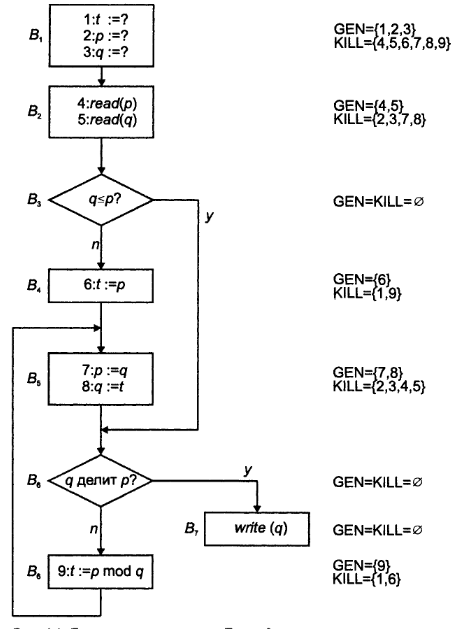
\includegraphics[scale=0.9] {4,1.png}}
	\caption{\textit{Блок-схема алгоритма Евклида}} 
\end{figure}

В общем случае \textit{анализ потока данных} относится к той части компилятора, которая проверяет блоковую структуру исходной программы (подобную рис. 4.1) и собирает 
информацию о выполнении операторов каждого прямоугольника блок-схемы.
\textit{Блоки} (прямоугольники) блок-схемы представляют совокупность операторов, через которые последовательно "проходит" поток данных. Информация, полученная в результате 
анализа потока данных, помогает повысить качество генерируемого компилятором кода программы. Если, например, в процессе анализа потока данных обнаружено, 
что при каждом прохождении блока \textit{B} переменная \textit{x} принимает значение 27, то можно подставить 27 для всех вхождений \textit{x} в блоке \textit{B} вместо 
выполнения оператора присваивания этой переменной. Если доступ к константам осуществляется быстрее, чем к значениям переменных, то описанная замена приводит к более 
эффективному коду программы, полученному в процессе компиляции.

В нашем примере мы хотим определить, где переменная последний раз принимала новое значение. Другими словами, мы хотим для каждого блока $\textit{B}_i$, вычислить
множество \textit{DEFIN[\textit{i}]} определений \textit{d} таких, которые сделаны в блоках от $\textit{B}_1$до $\textit{B}_i$, но
в последующих блоках нет других определений для той же переменной, которая определялась в определении \textit{d}.

Чтобы проиллюстрировать необходимость такой информации, рассмотрим блок-схему на рис. 4.1. Первый блок $\textit{B}_1$, являясь "холостым" блоком, содержит три 
определения, присваивающих переменным \textit{t, p}и \textit{q} "неопределенные" значения. Если, например, множество \textit{DEFIN[7]} включает в себя определение 3, которое присваивает
переменной \textit{q} "неопределенное" значение, значит, программа содержит ошибку, поскольку будет предпринята печать этой переменной без присваивания ей
"настоящего" значения. К счастью, в данной блок-схеме нетрудно проверить, что невозможно достигнуть блока $\textit{B}_7$, минуя операторы присвоения значений этой 
переменной, поэтому множество \textit{DEFIN[7]} не будет содержать определение 3.

При вычислении множества \textit{DEFIN[\textit{i}]} будем придерживаться нескольких правил.
Сначала для каждого блока $\textit{B}_i$, предварительно вычислим два множества \textit{GEN[\textit{i}]} и \textit{KILL[\textit{i}]}. \textit{GEN[\textit{i}]} — это множество определений, сделанных в блоке Д. Если в этом
блоке есть несколько определений одной переменной, то только последнее из них заносится в множество \textit{GEN[\textit{i}]}. Другими словами, \textit{GEN[\textit{i}]} является множеством 
определений, "генерируемых" блоком Д.

Множество \textit{KILL[\textit{i}]} содержит определения (из всех блоков, кроме Д) тех же переменных, которые определены в блоке $\textit{B}_i$,. Например, на рис. 4.1 GEN[4] — \{6\}, 
поскольку в блоке $\textit{B}_4$ содержится определение 6 (переменной \textit{t}). В свою очередь
\textit{KILL[4]}= \{1, 9\}, так как существуют определения 1 и 9 той же переменной \textit{t} и которые не входят в блок $\textit{B}_4$.

Кроме множеств \textit{DEFIN[\textit{i}]}, для каждого блока Д также будем вычислять множества \textit{DEFOUT[\textit{i}]}. Так же, как \textit{DEFIN[\textit{i}]} является множеством определений, действие
которых достигает блока Д, так и \textit{DEFOUT[\textit{i}]} — это множество определений, действие которых распространяется за блок $\textit{B}_i$,. Существует простая формула, 
связывающая множества \textit{DEFIN[\textit{i}]} и \textit{DEFOUT[\textit{i}]}:
\[
\textit{DEFOUT[i]} = (\textit{DEFIN[i]} - \textit{KILL[i}]) \cup GEN[i]  \tag*{(4.1)}
\]

Таким образом, определение \textit{d} распространяет свое действие за блок $\textit{B}_i$ только в двух
случаях: если его действие начато до блока Д и не "убито" в этом блоке или если оно генерировано в блоке $\textit{B}_i$. Вторая формула, связывающая множества \textit{DEFIN[\textit{i}]} и \textit{DEFOUT[\textit{i}]},
показывает, что \textit{DEFIN[\textit{i}]} можно вычислить как объединение тех множеств \textit{DEFOUT[\textit{p}]}, для которых определяющие их блоки $\textit{B}_p,$ предшествуют блоку $\textit{B}_i$.
\[
DEFIN[i] = \bigcup_{\textit{$B_p$ предшествует Д}} DEFOUT[p] \tag*{(4.2)}
\]
Из формулы (4.2) следует очевидный вывод, что определения данных регистрируются в блоке $\textit{B}_i$, тогда и только тогда, когда их действие начинается в одном из 
предшествующих блоков. В особых случаях, когда Д не имеет предшественников (как блок $\textit{B}_i$
на рис. 4.1), множество \textit{DEFIN[\textit{i}]} считается равным пустому множеству.


Хотя в этом примере введено много новых понятий, мы не будем обобщать этот материал для написания общих алгоритмов вычисления областей действия 
определений в произвольных блок-схемах. Вместо этого мы напишем часть программы вычисления множеств \textit{DEFIN[i]} и \textit{DEFOUT[i]} (\textit{i}=1,$\dots$, 8) для блок-схемы рис. 4.1,
предполагая, что множества \textit{GEN[i]} и \textit{KILL[i]} определены заранее. Отметим, что предлагаемый фрагмент программы предполагает существование АТД SET
(Множество) с операторами UNION, INTERSECTION, DIFFERENCE, EQUAL, ASSIGN и MAKENULL, позднее мы покажем, как реализовать этот АТД.

В создаваемом программном фрагменте (листинг 4.1) процедура \textit{propagate(GEN, KILL, DEFIN, DEFOUT)}\rindex{Программа!propagate} использует формулу (4.1) для вычисления множества
\textit{DEFOUT} указанного блока. Если программа свободна от циклов и повторяющихся структур, то в этом случае множества \textit{DEFOUT} можно вычислить непосредственно. 
При наличии в программе циклов или повторяющихся структур для вычисления \textit{DEFOUT} применяются итерационные процедуры. Сначала для всех \textit{i}
положим \textit{DEFIN[i]} = 0 и \textit{DEFOUT[i]} = \textit{GEN[i]}, затем последовательно применим формулы (4.1) и (4.2) несколько раз, пока не "стабилизируются" (не перестанут
изменяться) множества \textit{DEFIN} и \textit{DEFOUT}. Поскольку каждое новое значение множеств \textit{DEFIN[i]} и \textit{DEFOUT[i]} содержит свои предыдущие значения, а количество всех 
определений в программе ограничено, то процесс должен сходиться к решению уравнений (4.1) и (4.2).

Последовательные значения множеств \textit{DEFINli]} после каждой итерации цикла показаны в табл. 4.1. Заметим, что операторы 1, 2 и 3 присваивания переменным
"неопределенных" значений не распространяются на блоки, где эти переменные используются. Отметим также, что в листинге 4.2 сначала выполняются вычисления
по формуле (4.2), а затем по формуле (4.1); в общем случае это обеспечивает сходимость процесса вычисления \textit{DEFIN[i]} всего за несколько итераций. 

\fancyfoot[LO]{4.3. РЕАЛИЗАЦИЯ МНОЖЕСТВ ПОСРЕДСТВОМ ДВОИЧНЫХ ВЕКТОРОВ }
%%%%%%%%%4.1%%%%%%%%%%
\begin{lstlisting}[language=C, caption={ Программа вычисления областей действий операторов определения переменных}, numbers = none]
    SET GEN[8], KILL[8], DEFIN[8], DEFOUT[8];
    |	/* Предполагается, что GEN и KILL вычисляются  вне  этой  программы */  |
    int  i;
    bool changed;

    | /* Вычисления по формуле (4.1), переменная changed принимает значение |
                        | true, если есть изменения в DEFOUT */ |
    void propagate(const SET *G, *K, *I, SET *O) {
        SET TEMP;

        DIFFERENCE(I, K, &TEMP);
        UNION     (&TEMP, G, &TEMP);
        if (!EQUAL(&TEMP, O)) {
            ASSIGN(O, TMP);
            changed = true;
        }
    }
    int main(void) {
        for (i = 0; i < 8; ++i)
            ASSIGN(&DEFOUT[i], &GEN[i]);
        do {
            changed = false;

        |	/* Далее 8 операторов реализуют формулу (4.2), |
               |   но только для блок-схемы рис. 4.1 */ |

            MAKENULL(DEFIN[0]);
            ASSIGN(&DEFIN [1], &DEFOUT[0]);
            ASSIGN(&DEFIN [2], &DEFOUT[1]);
            ASSIGN(&DEFIN [3], &DEFOUT[2]);
            UNION (&DEFOUT[3], &DEFOUT[7], &DEFIN[4]);
            UNION (&DBFOUT[2], &DEFOUT[4], &DEFIN[5]);
            ASSIGN(&DEFIN [6], &DEFOUT[5]);
            ASSIGN(&DEFIN [7], &DEFOUT[5]);

            for (i = 0; i < 8; ++i)
                propagate(GEN + i, KILL + i, 
            DEFIN + i, DEFOUT + i);
        } 
        while (changed);
    }
\end{lstlisting}
\begin{onehalfspace}
\begin{table}[ht]
	\caption{Пример отношения между множеством студентов и множеством учебных курсов}
	\begin{center}
		\begin{tabular}{c|c|c|c|c}
			$\;$i$\;$ & Проход1 & Проход2 & Проход3 & Проход4  \\ \hline
			& \multicolumn{1}{|c|}{}  & \multicolumn{1}{c|}{}  & \multicolumn{1}{c|}{} \\[-0.8em]
			1 & O & O & O & O \\
			2 & \{1, 2, 3\} & \{1, 2, 3\} & \{1, 2, 3\} & \{1, 2, 3\} \\
			3 & \{4, 5\} & \{1, 4, 5\} & \{1, 4, 5\} & \{1, 4, 5\} \\
			4 & O & \{4, 5\} & \{1, 4, 5\} & \{1, 4, 5\} \\
			5 & \{6, 9\} & \{6, 9\} & \{4, 5, 6, 7, 8, 9\} & \{4, 5, 6, 7, 8, 9\} \\
			6 & \{7, 8\} & \{4, 5, 6, 7, 8, 9\} & \{1, 4, 5, 6, 7, 8, 9\} & \{1, 4, 5, 6, 7, 8, 9\} \\
			7 & O & \{7, 8\} & \{4, 5, 6, 7, 8, 9\} & \{1, 4, 5, 6, 7, 8, 9\} \\
			8 & O & \{7, 8\} & \{4, 5, 6, 7, 8, 9\} & \{1, 4, 5, 6, 7, 8, 9\}
		\end{tabular}
	\end{center}
\end{table}
\end{onehalfspace}
\section[Реализация множеств посредством двоичных векторов]{Реализация множеств посредством двоичных\\ векторов}\rindex{Множество!реализации}\rindex{Множество!реализация посредством двоичного вектора}

\normalsize 
\indent

Наилучшая конкретная реализация абстрактного типа данных SET\rindex{SET} (Множество) выбирается исходя из набора выполняемых операторов и размера множества. Если
все рассматриваемые множества будут подмножествами небольшого \textit{универсального множества}\rindex{Множество!универсальное} целых чисел 1, ..., \textit{N} для некоторого фиксированного \textit{N}, тогда можно
применить реализацию АТД SET посредством двоичного (булева)\rindex{Вектор!двоичный} вектора. В этой реализации множество представляется двоичным вектором, в котором \textit{i}-й бит равен
1 (или true), если \textit{i} является элементом множества. Главное преимущество этой реализации состоит в том, что здесь операторы MEMBER, INSERT и DELETE 
можно выполнить за фиксированное время (независимо от размера множества) путем прямой адресации к соответствующему биту. Но операторы UNION,
INTERSECTION и DIFFERENCE выполняются за время, пропорциональное размеру универсального множества.

Если универсальное множество так мало, что двоичный вектор занимает не более одного машинного слова, то операторы UNION, INTERSECTION и DIFFERENCE
можно выполнить с помощью простых логических операций (конъюнкции и дизъюнкции), выполняемых над двоичными векторами. В языке Pascal для представления небольших 
множеств можно использовать встроенный тип данных set. Максимальный размер таких множеств зависит от конкретного применяемого компилятора

\newpage

\noindent и поэтому не формализуем. Однако при написании программ мы не хотим быть связаны ограничением максимального размера множеств по крайней мере до тех пор,
пока наши множества можно трактовать как подмножества некоего универсального множества \{1, ..., \textit{N}\}. Поэтому в данном разделе будем придерживаться 
представления множества в виде булевого массива \textit{A}, где \textit{A[i]} = true тогда и только тогда, когда \textit{i} является элементом множества. 
С помощью объявлений языка Pascal АТД SET\rindex{SET!объявление} можно определить следующим образом:

\begin{lstlisting}[language=C, numbers = none]
    const N = /* |подходящее числовое значение|*/

    typedef bool * SET
\end{lstlisting}

Реализация оператора UNION приведена в листинге 4.2. Для реализации операторов INTERSECTION и DIFFERENCE надо в листинге 4.2 заменить логический оператор 
or на операторы and и and not соответственно. В качестве простого упражнения читатель может самостоятельно написать код для реализации других операторов, 
перечисленных в разделе 4.1 (за исключением операторов MERGE и FIND, которые не имеют практического смысла при данном представлении множеств).
%%%%%%%%%%%%%%%%4.2%%%%%%%%%%%%%%%%%%%%
\rindex{Реализация!операторов множеств}
\begin{lstlisting}[language=C, caption={ Реализация оператора UNION}, numbers = none]
    void UNION(const SET *A, const SET *B, SET *C) {
        int i;

        for (i = 0; i < N; ++i)
            C[i] = A[i] | or | B[i];
    }
\end{lstlisting}

Представление множеств в виде двоичных векторов можно применить не только тогда, когда универсальное множество состоит из последовательных целых чисел, но и в
более общей ситуации, когда универсальное множество конечно. Для этого достаточно установить взаимно однозначное соответствие между элементами этого множества и 
целыми числами 1, ..., \textit{N}. Например, так, как это сделано в примере 4.1, где вер определения данных мы пронумеровали числами от 1 до 9. В общем случае для реализации
такого отображения используется АТД MAPPING \rindex{MAPPING!объявление} (Отображение), описанный в главе 2. На практике обратное отображение из множества целых чисел в множество элементов
универсального множества проще выполнить с помощью массива \textit{A}, где \textit{A[i]} будет элементом универсального множества, соответствующим числу \textit{i}.

\section[Реализация множеств посредством связанных списков]{Реализация множеств посредством связанных \\ списков}\rindex{Множество!реализация посредством связанных списков}

\normalsize 
\indent

Очевиден способ представления множеств посредством связанных списков, когда элементы списка являются элементами множества. В отличие от представления
множеств посредством двоичных векторов, в данном представлении занимаемое множеством пространство пропорционально размеру представляемого множества, а
не размеру универсального множества. Кроме того, представление посредством связанных списков является более общим, поскольку здесь множества не обязаны быть
подмножествами некоторого конечного универсального множества.

При реализации оператора INTERSECTION (Пересечение) в рамках представления множеств посредством связанных списков есть несколько альтернатив. Если универсальное 
множество линейно упорядочено, то в этом случае множество можно представить в виде сортированного списка, т.е. предполагая, что все элементы множества
сравнимы посредством отношения "<", можно ожидать, что эти элементы в списке
будут находиться в порядке \textit{$e_1, e_2, \dots, e_n$}, когда \textit{$e_1 < e_2 < e_3 < \dots < e_n$}. Преимущество отсортированного списка заключается 
в том, что для нахождения конкретного элемента в списке нет необходимости просматривать весь список.

\fancyfoot[LO]{4.4. РЕАЛИЗАЦИЯ МНОЖЕСТВ ПОСРЕДСТВОМ СВЯЗАННЫХ СПИСКОВ }

Элемент будет принадлежать пересечению списков \textit{$L_1$} и \textit{$L_2$} тогда и только тогда, когда он содержится в обоих списках. 
В случае несортированных списков мы должны сравнить каждый элемент списка \textit{$L_1$} с каждым элементом списка \textit{$L_2$}, т.е. сделать порядка \textit{O($n^2$)}
операций при работе со списками длины п. Для сортированных списков операторы пересечения и некоторые другие выполняются сравнительно просто:
если надо сравнить элемент \textit{e} списка \textit{$L_1$} с элементами списка \textit{$L_2$}, то надо просматривать список \textit{$L_2$}
только до тех пор, пока не встретится элемент \textit{e} или больший, чем \textit{e}.
В первом случае будет совпадение элементов, второй случай показывает, что элемента \textit{e} нет в списке \textit{$L_2$}. 
Более интересна ситуация, когда мы знаем элемент \textit{d}, который в списке \textit{$L_1$} непосредственно предшествует элементу \textit{e}. 
Тогда для поиска элемента, совпадающего с элементом \textit{e}, в списке \textit{$L_2$} можно сначала найти такой элемент /, что \textit{d} $\leqslant$ \textit{f}, и начать просмотр списка \textit{$L_2$}
с этого элемента. Используя этот прием, можно найти совпадающие элементы в списках \textit{$L_1$} и \textit{$L_2$} за один проход этих списков, продвигаясь 
вперед по спискам в прямом порядке, начиная с наименьшего элемента. Код процедуры, реализующей оператор INTERSECTION, показан в листинге 4.3.
Здесь множества представлены связанными списками ячеек, чей тип определяется следующим образом:%%%%%%%%%%%%%%%%%%%%%
\begin{lstlisting}[language=C, numbers = none]
    typedef struct celltype_T {
        struct celltype_T *next;
        elementtype element;
    } celltype;
\end{lstlisting}

В листинге 4.3 предполагается, что elementtype — это тип целых чисел, которые можно упорядочить посредством обычного оператора сравнения <. Если elementtype
представлен другим типом данных, то надо написать функцию, которая будет определять, какой из двух заданных элементов предшествует другому элементу.
%%%%%%%%%%%%%%%
\begin{lstlisting}[language=C, caption={ Процедура INTERSECTION, использующая связанные \\списки}, numbers = none, keepspaces = true]
    /*  Вычисление пересечения сортированных списков А и В с 
    ячейками заголовков ahead и bhead, результат - сортированный 
    список, на чей заголовок указывает рс */
    void INTERSECTION(const cellltype *ahead, 
            const celltype *bhead, celltype *pc) {
    |/*  текущие ячейки списков А и В и последняя ячейка |
    |дополнительного списка С  */|
        celltype *acurrent, *bcurrent, *ccurrent;

        pc = new_celltype(); | /* создание заголовка для списка С */ |
        acurrent = ahead->next;
        bcurrent = bhead->next;
        ccurrent = pc;

        while (acurrent != NULL && bcurrent != NULL) {
    |/* сравнение текущих элементов списков А и В */ |
            if (acurrent->element == bcurrent->element) {
    |/* добавление элемента в пересечение */ |
                ccurrent->next = new_celltype();
                ccurrent = ccurrent->next;
                ccurrent->element = acurrent->element;
                acurrent = acurrent->next;
                bcurrent = bcurrent->next;
            }
            else{  |/* элементы неравны */ |
                if (acurrent->element < bcurrent->element)
                    acurrent = acurrent->next;
                else
                    bcurrent = bcurrent->next;
        }

        ccurrent->next = NULL;
    } /* INTERSECTION */
\end{lstlisting}

\fancyfoot[RE]{ГЛАВА 4. ОСНОВНЫЕ ОПЕРАТОРЫ МНОЖЕСТВ}

Связанные списки в листинге 4.3 в качестве заголовков имеют пустые ячейки, которые служат как указатели входа списков. Читатель при желании может написать 
эту программу в более общей абстрактной форме с использованием примитивов списков. Но программа листинга 4.3 может быть более эффективной, чем абстрактная 
программа. Например, в листинге 4.3 используются указатели на отдельные ячейки вместо "позиционных" переменных, указывающих на предыдущую ячейку.
Так можно сделать вследствие того, что элементы добавляются в список С, а списки А и В только просматриваются без вставки или удаления в них элементов.

Процедуру INTERSECTION листинга 4.3 можно легко приспособить для реализации операторов UNION и DIFFERENCE. Для выполнения оператора UNION надо все
элементы из списков \textit{A} и \textit{B} записать в список \textit{C}. Поэтому, когда элементы не равны (строки 12-14 в листинге 4.3), наименьший из них заносится в список \textit{C}, так же,
как и в случае их равенства. Элементы заносятся в список С до тех пор, пока на исчерпаются оба списка, т.е. пока логическое выражение в строке 5 не примет 
значение false. В процедуре DIFFERENCE в случае равенства элементов они не заносятся список \textit{C}. Если текущий элемент списка \textit{A} меньше текущего элемента списка \textit{B}, то
он (текущий элемент списка \textit{A}) заносится в список \textit{C}. Элементы заносятся в список \textit{C} до тех пор, пока не исчерпается список \textit{A} 
(логическое условие в строке 5).

Оператор ASSIGN (\textit{A}, \textit{B}) копирует список \textit{A} в список \textit{B}. Отметим, что этот оператор нельзя реализовать простым переопределением 
заголовка списка В на заголовок списка \textit{A}, поскольку при последующих изменениях в списке \textit{B} надо будет делать
аналогичные изменения в списке \textit{A}, что, естественно, может привести к нежелательным коллизиям. Оператор MIN реализуется легко — просто возвращается 
первый элемент списка. Операторы DELETE и FIND можно реализовать, применив общие методы поиска заданного элемента в списках, в случае оператора DELETE\rindex{Оператор!DELETE} найденный
элемент (точнее, ячейка, в которой он находится) удаляется.

Реализовать оператор вставки нового элемента в список также несложно, но он должен стоять не в произвольной позиции в списке, а в "правильной" позиции, учитывающей 
взаимный порядок элементов. В листинге 4.4 представлен код процедуры INSERT (Вставка), которая в качестве параметров имеет вставляемый элемент и 
указатель на ячейку заголовка списка, куда вставляется элемент. На рис. 4.2 показаны ключевые ячейки и указатели до и после вставки элемента 
(старые указатели обозначены сплошными линиями, а новые — пунктирными).
%%%%%%%%%%%%%
\begin{lstlisting}[language=C, caption={Процедура вставки элемента}, numbers = none]
    void INSERT (const |\textbf{elementtype}| *x, const |\textbf{celltype}| *p) {
        |\textbf{celltype}| *current, *newcell;
        current = p;
        while (current->next != NULL) {
            if (current->next->element == x)
                return; | /* элемент х уже есть в списке*/ |

            if (current->next->element > x)
                goto add; | /* далее останов процедуры*/ |

            current = current!->next
        };
        add:| /* здесь current — ячейка, после которой надо вставить х*/|
        newcell = new_celltype();
        newcell->element = х;
        newcell->next = currentt->next;
        current->next = newcell
    }; /* INSERT */
\end{lstlisting}


\fancyfoot[LO]{4.5 СЛОВАРИ}

\begin{figure}[ht]
	\center{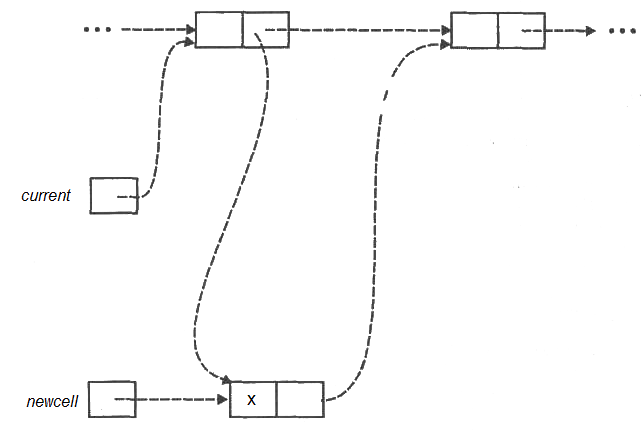
\includegraphics[scale=0.6] {4,2.png}}
	\caption{\textit{Схема вставки нового элемента}} 
\end{figure}

\section{Словари}

\normalsize 
\indent

Применение множеств при разработке алгоритмов не всегда требует таких мощных операторов, как операторы объединения и пересечения. Часто достаточно только
хранить в множестве "текущие" объекты с периодической вставкой или удалением некоторых из них. Время от времени также возникает необходимость узнать, 
присутствует ли конкретный элемент в данном множестве. Абстрактный тип множеств с операторами INSERT, DELETE и MEMBER называется DICTIONARY \rindex{DICTIONARY} (Словарь). Мы
также включим оператор MAKENULL в набор операторов словаря — он потребуется при реализации АТД для инициализации структур данных. Далее в этом разделе мы
приведем пример использования словарей, а в следующем разделе рассмотрим реали- зации, подходящие для представления словарей.

Пример 4.2. Общество защиты тунцов (ОЗТ) имеет базу данных с записями результатов самого последнего голосования законодателей по законопроектам об охране
тунцов. База данных состоит из двух списков (множеств) имен законодателей, которые названы \textit{goodguys} (хорошие парни) и \textit{badguys} (плохие парни). 
ОЗТ прощает законодателям их прошлые "ошибки", но имеет тенденцию забывать своих "друзей",
которые ранее голосовали "правильно". Например, после голосования по законопроекту об ограничении вылова тунца в озере Эри все законодатели, проголосовавшие за
этот законопроект, заносятся в список \textit{goodguys} и удаляются из списка \textit{badguys}, тогда как над оппонентами этого законопроекта совершается обратная процедура. 

\fancyfoot[RE]{ГЛАВА 4. ОСНОВНЫЕ ОПЕРАТОРЫ МНОЖЕСТВ}

Законодатели, не принимавшие участие в голосовании, остаются в тех списках, в которых они были ранее.

Для управления описываемой базы данных при вводе имен законодателей будем применять односимвольные команды, за символом команды будет следовать 10 
символов с именем законодателя. Каждая команда располагается в отдельной строке. Используем следующие односимвольные команды.
\begin{itemize}
	\item[1.]F (законодатель голосовал "правильно").
	\item[2.]U (законодатель голосовал "неправильно").
	\item[3.]? (надо определить статус законодателя).
\end{itemize}

Мы также будем использовать символ 'Е' для обозначения окончания процесса ввода списка законодателей. В листинге 4.5 показан эскиз программы tuna\rindex{Программа!tuna} (тунец), написанный в терминах пока не определенного АТД DICTIONARY \rindex{DICTIONARY} (Словарь), который в данном случае можно представить как множество символьных строк длиной 10.

%%%%%%%%%%%%%%%%%%%%%%%%
\begin{lstlisting}[language=C, caption={  Программа управления базой данных ОЗТ}, numbers = none]
|/* База данных законодателей (legislator)*/ |
    char nametype[10];
    char command;
    |\textbf{nametype}|  legislator;
    DICTIONARY goodguys, badguys;

|/* заносит имя friend (друг) в список goodguys и вычеркивает из списка badguys*/|
    void favor (|\textbf{nametype}| *friend) {
        INSERT(friend, goodguys);
        DELETE(friend, badguys)
    }; /* favor */

|/* заносит имя foe (враг) в список badguys и вычеркивает из списка goodguys*/ |
    void unfavor (|\textbf{nametype}| *foe) {
        INSERT(foe, badguys);
        DELETE(foe, goodguys)
    }; /* unfavor */

|/* печать имени subject с соответствующей характеристикой*/|
    void report (nametype *subject) {
        if (MEMBER(subject, goodguys))
            pritnf(" \%s — это друг\n ", subject)
        else if (MEMBER(subject, badguys))
            pritnf("\%s — это друг\n", subject)
        else
            pritnf("|Нет данных о |\%s\n", subject);
    }; /* report */

    int main(void) {
        /* основная программа */ 
        MAKENULL(goodguys);
        MAKENULL(badguys);

        scanf("\%c", &command);

        while (command != 'E')  {
            readln(legislator);

            if (command == 'F')
                favor(legislator)
            else if (command == 'U')
                unfavor(legislator);
            else if (command == '?')
                report(legislator);
            else
                report('|Неизвестная команда|')
            scanf("\%c", &command);
        }
    }; /* tuna */ 
\end{lstlisting}


\fancyfoot[LO]{4.6. РЕАЛИЗАЦИИ СЛОВАРЕЙ }

\section{Реализации словарей}\rindex{Реализация!операторов словарей}\rindex{Реализация!словарей}
\rindex{Словари!реализация}
\normalsize 
\indent

Словари можно представить посредством сортированных или несортированных\\ связанных списков. Другая возможная реализация словарей использует двоичные
векторы, предполагая, что элементы данного множества являются целыми числами 1, ..., \textit{N} для некоторого \textit{N} или элементы множества можно сопоставить с таким
множеством целых чисел.

Третья возможная реализация словарей использует массив фиксированной длины с указателем на последнюю заполненную ячейку этого массива. Эта реализация выполнима, 
если мы точно знаем, что размер множества не превысит заданную длину массива. Эта реализация проще реализации посредством связанных списков, но имеет 
следующие недостатки: множества могут расти только до определенной фиксированной величины; медленно выполняются операции удаления элементов из множества 
(так как требуется перемещение оставшихся элементов массива) и невозможность эффективно организовать пространство массивов (особенно если множества имеют
различные размеры).

Так как мы рассматриваем реализации именно словарей (и вследствие последнего приведенного недостатка), то не будем затрагивать возможности выполнения в 
реализации посредством массивов операций объединения и пересечения множеств. Вместе с тем, поскольку массивы, так же, как и списки, можно сортировать, 
то читатель вправе рассматривать реализацию с помощью массивов (которую мы здесь применяем только для представления словарей) в качестве приемлемой реализации 
множеств произвольной структуры. В листинге 4.6 приведены объявления и процедуры, являющиеся необходимым дополнением программы листинга 4.5, — вместе с этими
дополнениями программа должна работать.

%%%%%%%%%%%%%
\begin{lstlisting}[language=C, caption={Объявления типов и процедуры реализации словаря посредством массива}, numbers = none]
    const size_t maxsize == |/* некое число, максимальный размер массива */|;

    typedef struct {
        int last;
        |\textbf{nametype}| data[maxsize];
    } DICTIONARY;

    void MAKENULL (|\textbf{DICTIONARY}| *A) {
        A->last = -1;
    }; /* MAKENULL */

    bool MEMBER (const |\textbf{nametype}| *x, |\textbf{DICTIONARY}| *A) {
        int i;

        for (i = 0; i <= A->last; ++i)
            if (A->data[i] == x)
                return true;

        return false;| /* элемент x не найден */|
    }; /* MEMBER */

    void INSERT (const |\textbf{nametype}| *x, |\textbf{DICTIONARY}| *A) {
        if (!MEMBER(x, A)) {
            if (A->last < maxsize - 1)  {
                A->last = A->last + 1;
                A->data[A->last] = *x;
            }
            else
                error("База данных заполнена");
        }
    }; /* INSERT */

    void DELETE (const |\textbf{nametype}| *x, |\textbf{DICTIONARY}| *A) {
        int i;

        if (A->iast > 0) {
            i = 1;

            while (A->data[i] != x && i < A->last)
                i = i + 1;

            if (A->datali] == *x)  {
                A->data[i] == A->data[A->last];
    |/* перемещение последнего элемента на место |
    |    элемента х; если i == A->last, то  |
    |   удаление х происходит на следующем шаге */|
                A->last = A->last - i; /* или 1 ?.... */
            }
        }
    }; /* DELETE */
\end{lstlisting}


\fancyfoot[LO]{4.7. СТРУКТУРЫ ДАННЫХ, ОСНОВАННЫЕ НА ХЕШ-ТАБЛИЦАХ}
\section{Структуры данных, основанные на хеш-таблицах}

\normalsize 
\indent

В реализации словарей с помощью массивов выполнение операторов INSERT,\\ DELETE и MEMBER требует в среднем \textit{O(N)} выполнений элементарных инструкций
для словаря из \textit{N} элементов. Подобной скоростью выполнения операторов обладает и реализация с помощью списков. 
При реализации словарей посредством двоичных векторов все эти три оператора выполняются за фиксированное время независимо от
размера множеств, но в этом случае мы ограничены множествами целых чисел из некоторого небольшого конечного интервала.

Существует еще один полезный и широко используемый метод реализации словарей, который называется \textit{хешированием} \rindex{Хеширование}. Этот метод требует фиксированного 
времени (в среднем) на выполнение операторов и снимает ограничение, что множества должны быть подмножествами некоторого конечного универсального множества. 
В самом худшем случае этот метод для выполнения операторов требует времени, 



\noindent пропорционального размеру множества, так же, как и в случаях реализаций посредством массивов и списков. Но при тщательной разработке алгоритмов мы 
можем сделать так, что вероятность выполнения операторов за время, большее фиксированного, будет как угодно малой.

Мы рассмотрим две различные формы хеширования. 
Одна из них называется \textit{открытым}\rindex{Хеширование!открытое}, или \textit{внешним хешированием} и позволяет хранить множества в 
потенциально бесконечном пространстве, снимая тем самым ограничения на размер множеств. Другая называется \textit{закрытым} \rindex{Хеширование!закрытое}, или \textit{внутренним хешированием} 
\footnote[1]{ Есть несколько классификаций методов хеширования по разным признакам. Мы оставляем здесь классификацию (и терминологию) авторов, поскольку она проста и непротиворечива.
	Отметим только, что открытое хеширование, как оно изложено далее, является частным случаем так называемого \textit{расширенного хеширования}, а закрытое хеширование часто называют
	\textit{прямым хешированием}. — Прим. ред.} и использует ограниченное пространство для хранения данных, ограничивая таким образом размер множеств \footnote[2]{Путем внесения изменений в 
	структуру данных можно изменять объем пространства, занимаемого данными при открытом хеширование, и увеличить его при закрытом хешировании.
	Мы опишем эти технологии после знакомства с основными методами хеширования.}.

\subsection*{Открытое хеширование}
\addcontentsline{toc}{subsection}{ Открытое хеширование } 
\indent

На рис. 4.3 показана базовая структура данных при открытом хешировании. Основная идея заключается в том, что потенциальное множество (возможно, бесконечное) 
разбивается на конечное число классов. Для \textit{B} классов, пронумерованных от О до $B - 1$, строится \textit{хеш-функция h}\rindex{Хеширование!хеш-функция} \rindex{Хеш-функция} такая, что для любого элемента \textit{x} исходного множества 
функция $h(x)$ принимает целочисленное значение из интервала $0, ..., B -1$, которое, естественно, соответствует классу, которому принадлежит элемент $x$. 
Элемент $x$ часто называют ключом, $h(x)$ — хеш-значением $x$ \rindex{Хеширование!хеш-значение}, а "классы" — сегментами\rindex{Хеширование!сегменты}. Мы будем говорить, что элемент $x$ принадлежит сегменту $h(x)$.
\begin{figure}[ht!]
	\center{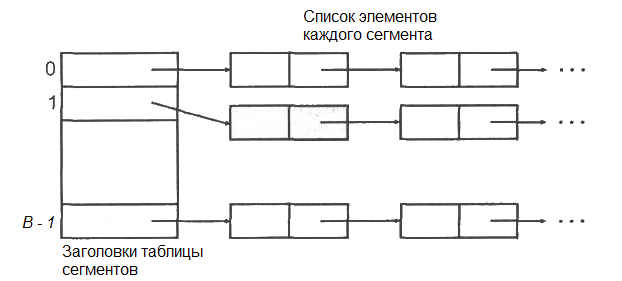
\includegraphics[scale=0.8] {4,3.png}}
	\caption{\textit{Организация данных при открытом хешировании}} 
\end{figure}

Массив, называемый таблицей сегментов и проиндексированный номерами сегментов $ 0, 1,..., B - 1 $, содержит заголовки для \textit{B} списков. Элемент \textit{x} \textit{i}-ro списка —
это элемент исходного множества, для которого $h(x) = i$.

Если сегменты примерно одинаковы по размеру, то в этом случае списки всех сегментов должны быть наиболее короткими при данном числе сегментов. Если исходное 
множество состоит из \textit{N} элементов, тогда средняя длина списков будет $N \backslash B$ элементов. Если можно оценить величину \textit{N} и выбрать \textit{B} как можно ближе к этой
величине, то в каждом списке будет один-два элемента. Тогда время выполнения операторов словарей будет малой постоянной величиной, зависящей от \textit{N}(или, что
эквивалентно, от \textit{B}).

\fancyfoot[RE]{ГЛАВА 4. ОСНОВНЫЕ ОПЕРАТОРЫ МНОЖЕСТВ}
Не всегда ясно, как выбрать хеш-функцию \textit{A} так, чтобы она примерно поровну распределяла элементы исходного множества по всем сегментам. Ниже мы покажем
простой способ построения функции \textit{A}, причем $h(x)$ будет "случайным" значением, почти независящим от \textit{x}.

Здесь же мы введем хеш-функцию (которая будет "хорошей", но не "отличной"), определенную на символьных строках. Идея построения этой функции заключается в
том, чтобы представить символы в виде целых чисел, используя для этого машинные коды символов. В языке Pascal \rindex{Pascal} есть встроенная функция \textit{ord(c)}, которая возвращает
целочисленный код символа \textit{c}. Таким образом, если \textit{x} — это ключ, тип данных ключей определен как аггау[1..10] of char (в примере 4.2 этот тип данных назван nametype),
тогда можно использовать хеш-функцию, код которой представлен в листинге 4.7. В этой функции суммируются все целочисленные коды символов, результат суммирова-
ния делится на \textit{B} и берется остаток от деления, который будет целым числом из интервала от $ 0 $ до $B - 1$.

%%%%%%%%%%%
\begin{lstlisting}[language=C, caption={ Простая хеш-функция}, numbers = none]
    int h (const |\textbf{nametype}| *х) {
        int i, sum = 0;

        for (i = 0; i < 10; ++i)
            sum = sum + x[i];

        return sum % В;
    }; /* h */
\end{lstlisting}

В листинге 4.8 показаны объявления структур данных для открытой хеш-таблицы и процедуры, реализующие операторы, выполняемые над словарем. Тип
данных элементов словаря — nametype (здесь — символьный массив), поэтому данные объявления можно непосредственно использовать в примере 4.2. Отметим, что в
листинге 4.8 заголовки списков сегментов сделаны указателями на ячейки, а не "настоящими" ячейками. Это сделано для экономии пространства, занимаемого данными: 
если заголовки таблицы сегментов будут ячейками массива, а не указателями, то под этот массив необходимо столько же места, сколько и под списки элементов.
Но за такую экономию пространства надо платить: код процедуры DELETE должен уметь отличать первую ячейку от остальных.
\rindex{Словари!реализация посредством открытого хеширования}
\begin{lstlisting}[language=C, caption={ Реализация словарей посредством открытой хеш-таблицы}, numbers = none]
    const В =| /* подходящая константа */|;

    typedef struct celltype_T {
        nametype element;
        celltype_T *next;
    } celltype;

    |\textbf{celltype}| DICTIONARY[B];

    void MAKENULL (|\textbf{DICTIONARY}| A ) {
        int i;

        for (i = 0; i < B; ++i;)
            A [i] = NULL;
    }; /* MAKENULL */

    bool MEMBER (const |\textbf{nametype}| *x, |\textbf{DICTIONARY}| *A) {
        |\textbf{celltype}| *current;

        current = A[h(x)];
        |/* начальное значение current равно заголовку сегмента, которому |
        |    принадлежит элемент х */|

        while (current != NULL)
            if (current->element == x)
                return true;
            else
                current = current->next ;
    
        return false;| /* элемент х не найден */|
    };| /* MEMBER */|

    void INSERT ( const |\textbf{nametype}| *x, |\textbf{DICTIONARY}| *A) {
        int bucket;| /* для номера сегмента */|
        celltype *oldheader;

        if (!MEMBER(x, A)) {
            bucket = h(x);
            oldheader = A[bucket];
            A[bucket] = new_celltype();
            A[buaket]->element = x;
            Albucket]->next = oldheader
        }
    };|/* INSERT */|

    void DELETE ( const |\textbf{nametype}| *x, |\textbf{DICTIONARY}| *A) {
        int bucket;
        |\textbf{celltype}| *t;

        bucket = h(x);

        if (A[bucket] != NULL)  {
            if (A[bucket]->element == x)  |/* x в первой ячейке */|
                A[bucket] = A[bucket]->next; 
                |/* удаление х из списка */|
            else {| /* x находится не в первой ячейке */|
                current = A[bucket];
                |/* current указывает на предыдущую ячейку */|
            while (currentt->next != NULL)
                if (current->next->element == x)  {
                    current->next = current->next->next;
                    |/* удаление х из списка */|
                    return;| /* останов */|
                }
                else |/* x пока не найден */|
                    current = current->next;
            }
        }
    }; |/* DELETE */|
\end{lstlisting}



\fancyfoot[RE]{ГЛАВА 4. ОСНОВНЫЕ ОПЕРАТОРЫ МНОЖЕСТВ}

\subsection*{Закрытое хеширование} \rindex{Хеширование!закрытое, анализ}
\addcontentsline{toc}{subsection}{ Закрытое хеширование}
\normalsize 
\indent

При закрытом хешировании в таблице сегментов хранятся непосредственно элементы словаря, а не заголовки списков. Поэтому в каждом сегменте может храниться 
только один элемент словаря. При закрытом хешировании применяется методика \textit{повторного хеширования}\rindex{Хеширование!повторное}. Если мы попытаемся поместить элемент \textit{x} в сегмент с номером 
$h(x)$, который уже занят другим элементом (такая ситуация называется коллизией), то в соответствии с методикой повторного хеширования выбирается 
последовательность других номеров сегментов $h_1(x), h_2(x), ...$, куда можно поместить элемент \textit{x}. Каждое из этих местоположений последовательно проверяется, пока не будет
найдено свободное. Если свободных сегментов нет, то, следовательно, таблица заполнена и элемент \textit{x} вставить нельзя.

Пример 4.3. Предположим, что $B = 8$ и ключи \textit{а, b, с} и \textit{d} имеют хеш-значения
$h(a) = 3, h(b) = 0, h(c) = 4 $ и $ h(d) = 3 $. Применим простую методику, которая называется \textit{линейным хешированием}\rindex{Хеширование!линейное}. При линейном хешировании
$ h_i(x) - (h(x) + i) mod B $. Например, если мы хотим 
вставить элемент \textit{d}, a сегмент 3 уже занят, то можно проверить на занятость 
сегменты 4, 5, 6, 7, 0, 1 и 2 (именно в таком порядке).

Мы предполагаем, что вначале вся хеш-таблица пуста, т.е. в каждый сегмент помещено специальное значение \textit{empty} (пустой), которое не совпадает ни с одним 
элементом словаря \footnote[1]{Если тип данных элементов словаря не соответствует типу значения empty, то в каждый
	сегмент можно поместить дополнительное однобитовое поле с маркером, показывающим, занят или нет данный сегмент.}.
Теперь последовательно вставим элементы \textit{а, b, с} и \textit{d} в пустую таблицу: элемент \textit{a} попадет в сегмент 3, элемент \textit{b} — в сегмент 0, а элемент \textit{c} — в сегмент 4. 
Для элемента \textit{d} $ h(d) - 3$, но сегмент 3 уже занят. 
Применяем функцию $h_1: h_1(d) = 4$, но сегмент 4 также занят. Далее применяем функцию 
$h_2: h_2(d) = 5$, сегмент 5 свободен, помещаем туда элемент \textit{d}. Результат заполнения хеш-таблицы показан на рис. 4.4.

\begin{figure}[ht!]
	\center{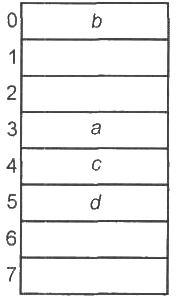
\includegraphics[scale=0.7] {4,4.png}}
	\caption{\textit{Частично заполненная хеш-таблица}} 
\end{figure}

При поиске элемента \textit{x} (например, при выполнении оператора MEMBER) необходимо просмотреть все местоположения $h(x), h_1(x), h_2(x), ...$, пока не будет найден \textit{x}
или пока не встретится пустой сегмент. Чтобы объяснить, почему можно остановить поиск при достижении пустого сегмента, предположим, что в словаре не допускается
удаление элементов. И пусть, для определенности, $h_3(x)$ — первый пустой сегмент. В такой ситуации невозможно нахождение элемента \textit{x} в сегментах $h_4(x), h_5(x)$ и далее,

\newpage
\fancyfoot[LO]{4.7. СТРУКТУРЫ ДАННЫХ, ОСНОВАННЫЕ НА ХЕШ-ТАБЛИЦАХ}


\noindent так как при вставке элемент х вставляется в первый пустой сегмент, следовательно, он находится где-то до сегмента $h_3(x)$.

Но если в словаре допускается удаление элементов, то при достижении пустого сегмента мы, не найдя элемента \textit{x}, не можем быть уверенными в том, что его вообще
нет в словаре, так как сегмент может стать пустым уже после вставки элемента \textit{x}. Поэтому, чтобы увеличить эффективность данной реализации, необходимо 
в сегмент, который освободился после операции удаления элемента, поместить специальную константу, которую назовем \textit{deleted} (удаленный). Важно различать константы 
\textit{deleted} и \textit{empty} — последняя находится в сегментах, которые никогда не содержали элементов. При таком подходе (даже при возможности удаления 
элементов) выполнение оператора MEMBER не требует просмотра всей хеш-таблицы. Кроме того, при вставке элементов сегменты, помеченные константой \textit{deleted}, 
можно трактовать как свободные, таким образом, пространство, освобожденное после удаления элементов, можно рано или поздно использовать повторно. 
Но если невозможно непосредственно сразу после удаления элементов пометить освободившееся сегменты, то следует предпочесть закрытому хешированию схему открытого хеширования.

Пример 4.4. Предположим, что надо определить, есть ли элемент \textit{e} в множестве, представленном на рис. 4.4. Если $h(e)$ — 4, то надо проверить еще сегменты 
4, 5 и затем сегмент 6. Сегмент 6 пустой, в предыдущих просмотренных сегментах элемент \textit{e} не найден, следовательно, этого элемента в данном множестве нет.

Допустим, мы удалили элемент \textit{с} и поместили константу \textit{deleted} в сегмент 4. В этой ситуации для поиска элемента \textit{d} мы начнем с просмотра сегмент $h(d) = 3$, затем
просмотрим сегменты 4 и 5 (где и найдем элемент \textit{d}), при этом мы не останавливаемся на сегменте 4 — хотя он и пустой, но не помечен как \textit{empty}.

В листинге 4.9 представлены объявления типов данных и процедуры операторов для АТД DICTIONARY с элементами типа nametype и реализацией, использующей
закрытую хеш-таблицу. Здесь используется хеш-функция Л из листинга 4.7, для разрешения коллизий\rindex{Хеширование!разрешение коллизий} применяется методика линейного хеширования. Константа
\textit{empty} определена как строка из десяти пробелов, а константа \textit{deleted} — как строка из десяти символов "*", в предположении, что эти строки не совпадают ни с одним
элементом словаря. (В базе данных примера 4.2 эти строки, очевидно, не будут совпадать с именами законодателей.) Процедура INSERT(\textit{x}, Л) использует функцию
\textit{locate} (местонахождение) для определения, присутствует ли элемент \textit{x} в словаре \textit{A} или нет, а также специальную функцию \textit{locate1} для определения местонахождения
элемента \textit{x}. Последнюю функцию также можно использовать для поиска констант \textit{deleted} и \textit{empty}.
\rindex{Словари!реализация посредством закрытого хешироания}
\begin{lstlisting}[language=C, caption={Реализация словаря посредством закрытого хеширования}, numbers = none]
    const char * empty   = "          "; #|10 пробелов|
    const char * deleted = "**********"; #|10 символов *|

    typedef nametype * DICTIONARY;

    void MAKENULL ( |\textbf{DICTIONARY}| *A ) {
        int i;
        for (i = 0; i < В; ++i)
            A[i] = empty;
    } //|MAKENULL|

    int locate ( const |\textbf{nametype}| *x, |\textbf{DICTIONARY}| *A ) {
    /* |Функция просматривает $A$ начиная от сегмента $h(x)$ до тех пор,|
        |пока не будет найден элемент $x$ или не встретится пустой сегмент| 
        |или пока не будет достигнут конец таблицы|
        |(в последних случаях принимается, что таблица не содержит|
        |элемент $x$). Функция возвращает позицию,| 
        |в которой остановился поиск.|*/
        int initial, i;

        initial = h(x);
        i = 0;

        while ((i < B) && (A[(initial + i) rood B] != x) && 
        (A[(initial + i) \% В != empty)) #|!!!|
            i = i + 1;

        return((initial + i) % B)
    } #|locate|

    int locate1 ( const |\textbf{nametype}| *x, |\textbf{DICTIONARY}| *A);
        /* |To же самое, что и функция $locate$, но останавливается и при|
        |достижении значения $deleted$| */

    bool MEMBER ( const |\textbf{nametype}| *x, |\textbf{DICTIONARY}| *A ) {
        if ( A[locate(x)] == x)
            return true;
        else
            return false;
    } #|MEMBER|

    void INSERT (const |\textbf{nametype}| *x, |\textbf{DICTIONARY}| *A) {
        int	bucket;

        if ( A[locate(x)] == x)
            return; /* |$x$ уже есть в $A$| */
        bucket = locatel(x);
        if ( (A[bucket] == empty) || (A[bucket] == deleted))
            A[bucket] = x
        else
            printf("|Операция INSERT невозможна: таблица полна|");
    } /* |INSERT| */

    void DELETE ( const |\textbf{nametypedef}| *x; |\textbf{DICTIONARY}| *A ) {
        int bucket;

        bucket = locate(x);
        if ( A[locate(x)] == x)
            A[bucket] = deleted
    } /|* DELETE *|/
\end{lstlisting}

\section{Оценка эффективности хэш-функций}

\normalsize 
\indent

Напомним, что хеширование - эффективный способ представления словарей и
некоторых других абстрактных типов данных, основанных на множествах. В этом
разделе мы оценим среднее время выполнения операторов словарей для случая открытого хеширования. Если есть \textit{B} сегментов и $N$ элементов, хранящихся в хеш-таблице,

\fancyfoot[RE]{ ГЛАВА 4. ОСНОВНЫЕ ОПЕРАТОРЫ МНОЖЕСТВ}


\noindent то каждый сегмент в среднем будет иметь $N/B$ элементов и мы ожидаем,
что операторы INSERT, DELETE и MEMBER будут выполняться в среднем \textit{за} время $O(1 + N/B)$. Здесь константа 1 соответствует поиску сегмента, а \( N/B \) - поиску
элемента в сегменте. Если $B$ примерно равно $N$, то время выполнения операторов
становится константой, независящей от $N$.

Предположим, что есть программа, написанная на языке программирования, подобном Pascal, и мы хотим все имеющиеся в этой программе идентификаторы занести в хеш-таблицу. После обнаружения объявления нового идентификатора он вставляется в хеш-таблицу, конечно же, после проверки, что его еще нет в хеш-таблице.
На этапе проверки естественно предположить, что идентификатор с равной вероятностью может быть в любом сегменте. Таким образом, на процесс заполнения хеш-
таблицы с $N$ элементами потребуется время порядка $O(N(1 + N/B))$. Если положить,
что \textit{B} равно $N$, то получим время $O(N)$.

На следующем этапе анализа программы просматриваются идентификаторы в
теле программы. После нахождения идентификатора в теле программы, чтобы получить информацию о нем, его же необходимо найти в хеш-таблице. Какое время
потребуется для нахождения идентификатора в хеш-таблице? Если время поиска
для всех элементов примерно одинаково, то оно соответствует среднему времени
вставки элемента в хеш-таблицу. Чтобы увидеть это, достаточно заметить, что
время поиска любого элемента равно времени вставки элемента в конец списка соответствующего сегмента. Таким образом, время поиска элемента в хеш-таблице
составляет \textit{О}$(1 + N/B)$.

В приведенном выше анализе предполагалось, что хеш-функция распределяет
элементы по сегментам равномерно. Но существуют ли такие функции? Рассмотрим
функцию, код которой приведен в листинге 4.7, как типичную хеш-функцию.
(Напомним, что эта функция преобразует символы в целочисленный код, суммирует
коды всех символов и в качестве результата берет остаток от деления этой суммы на
число \textit{В}.) Следующий пример оценивает работу этой функции.

Пример 4.5. Предположим, что функция из листинга 4.7 применяется для занесения в таблицу со 100 сегментами 100 символьных строк АО, А1, ..., А99\footnote[1]{Отметим, что строки А2 и А20 не обязательно должны находиться в одном сегменте, но
	А23 и А41, например, будут располагаться в одном сегменте.}. Принимая во внимание, что \textit{ord(O), ord(l) ord(9)} образуют арифметическую прогрессию
(это справедливо для всех таблиц кодировок, где цифры 0, ..., 9 стоят подряд, например для кодировки ASCII), легко проверить, что эти элементы займут не более 29
сегментов из ста , наибольший сегмент (сегмент с номером 2) будет содержать элементы А18, А27, А36, ..., А90, т.е. девять элементов из ста\footnote[2]{Обратите внимание, что здесь "А" — буква английского алфавита и что приведенное распределение элементов по сегментам справедливо только для записанных выше символьных
	строк. Для другой буквы (или других символьных строк) получим другое распределение элементов по сегментам, но также, скорее всего, далекое от равномерного. - Прим. ред.}. Используя тот факт,
что для вставки \textit{i-ro} элемента требуется $i + 1$ шагов, легко подсчитать, что в данном
случае среднее число шагов, необходимое для вставки всех 100 элементов, равно 395.
Для сравнения заметим, что оценка $N(1 + N/B)$ предполагает только 200 шагов. $\square$

В приведенном примере хеш-функция распределяет элементы исходного множества по множеству сегментов не равномерно. Но возможны "более равномерные" хеш-
функции. Для построения такой функции можно воспользоваться хорошо известным
методом возведения числа в квадрат и извлечения из полученного квадрата нескольких средних цифр. Например, если есть число $n$, состоящее из 5 цифр, то после возведения его в квадрат получим число, состоящее из 9 или 10 цифр. $"$Средние цифры$"$ - это цифры, стоящие, допустим, на позициях от 4 до 7 (отсчитывая справа).
Их значения, естественно, зависят от числа $n$. Если \textit{В} = 100, то для формирования
номера сегмента достаточно взять две средние цифры, стоящие, например, на позициях 5 и 6 в квадрате числа.

\fancyfoot[LO]{4.8. ОЦЕНКА ЭФФЕКТИВНОСТИ ХЕШ-ФУНКЦИЙ}



Этот метод можно обобщить на случай, когда В не является степенью числа 10.
Предположим, что элементы исходного множества являются целыми числами из
интервала О, 1, ..., К. Введем такое целое число С, что $\textit{ВС}{^2}$ примерно равно $\textit{К}{^2}$,
тогда функция

\[
h(n) = [n^2/C] mod B
\]

\noindent где $[x]$  обозначает целую часть числа $x$, эффективно извлекает из середины числа $n^2$
цифры, составляющие число, не превышающее $B$.

Пример 4.6. Если $K = 1000$ и $ B = 8 $, то можно выбрать $C = 354$. Тогда

\[
A(456) = \Big[\frac{207936}{354}\Big]mod 8 = 587mod  8  =  3 \tag*{$\Box$}
\]

Для применения к символьной строке описанной хеш-функции надо сначала в
строке сгруппировать символы справа налево в блоки с фиксированным количеством
символов, например по 4 символа, добавляя при необходимости слева пробелы. Каждый блок трактуется как простое целое число, из которого путем конкатенации
(сцепления) формируется двоичный код символов, составляющих блок. Например, основная таблица ASCII кодировки символов использует 7-битовый код, поэтому символы
можно рассматривать как "цифры" по основанию $2{^2}$ или 128\footnote[1]{ Конечно, если вы работаете не только с латиницей, но и с кириллицей, то необходимо использовать полную таблицу ASCII. В этом случае основанием для $"$цифр$"$-символов будет не $2{^7}$, а $2{^8}$, но суть метода от этого не меняется. - Прим. ред.}. Таким образом, символьную строку abed можно считать целым числом \textit{(128$){^3}$а + (128$){^2}$b + (128)с + d}. После
преобразования всех блоков в целые числа они суммируются\footnote[2]{ Если исходные символьные строки очень длинные, то суммирование можно выполнять по
	модулю некоторой константы с. Эту константу можно взять большей любого числа, получающегося из простого блока символов.}, а затем выполняется
вышеописанный процесс возведения в квадрат и извлечения средних цифр.

\subsection*{Анализ закрытого хеширования} \rindex{Анализ!закрытого хэширования}
\addcontentsline{toc}{subsection}{ Анализ закрытого хеширования}
\normalsize 
\indent

В случае применения схемы закрытого хеширования скорость выполнения вставки и других операций зависит не только от равномерности распределения элементов
по сегментам хеш-функцией, но и от выбранной методики повторного хеширования
для разрешения коллизий, связанных с попытками вставки элементов в уже заполненные сегменты. Например, методика линейного хеширования для разрешения
коллизий -  не самый лучший выбор. Не приводя в данной книге полного решения
этой проблемы, мы ограничимся следующим анализом.

Как только несколько последовательных сегментов будут заполнены (образуя \\группу), 
любой новый элемент при попытке вставки в эти сегменты будет 
вставлен в конец этой группы, увеличивая тем самым длину группы последовательно заполненных сегментов. Другими словами, для поиска пустого сегмента в случае непрерывного расположения заполненных сегментов необходимо просмотреть больше сегментов,
чем при случайном распределении заполненных сегментов. Отсюда также следует
очевидный вывод, что при непрерывном расположении заполненных сегментов увеличивается время выполнения вставки нового элемента и других операторов.

Определим, сколько необходимо сделать \textit{проб} (проверок) на заполненность сегментов при вставке нового элемента, предполагая, что в хеш-таблице, состоящей из \textit{В}
сегментов, уже находится \textit{N} элементов и все комбинации расположения \textit{N} элементов
в \textit{В} сегментах равновероятны. Это общепринятые предположения, хотя не доказано,
что схемы, отличные от схем закрытого хеширования, могут дать в среднем лучшее
время выполнения операторов словарей. Далее мы получим формулы, оценивающие
"стоимость" (количество проверок на заполненность сегментов) вставки нового элемента, если сегменты выбираются случайным образом. Наконец, мы рассмотрим некоторые методики повторного хеширования, дающие "случайное" (равномерное) распределение элементов по сегментам.



Вероятность коллизии равна \textit{N/B}. Предполагая осуществление коллизии, на
первом этапе повторного хеширования "работаем" с \textit{В - 1} сегментом, где находится \textit{N - 1} элемент. Тогда вероятность возникновения двух подряд коллизий
равна $N(N - 1)/($В(В$ - 1))$. Аналогично, вероятность по крайней мере $i$ коллизий равна

\[
\frac{N(N - 1)...(N - i +1)}{B(B - 1)...(B - i + 1)}\tag{4.3}
\]

Если значения \textit{В} к \textit{N} большие, то эта вероятность примерно равна \textit{(N/B$){^i}$}. 
Среднее числo проб равно единице плюс сумма по всем i > 1 вероятностей событий, что, по крайней мере, осуществится $i$ коллизий, 
т.е. среднее число проб примерно равно (не превышает) \(1 + \sum\limits_{i = 1}^{\infty}{(N/B)^i} = \frac{B}{B - N}\)\footnote[1]{ Здесь использована следующая формула вычисления среднего (математического ожидания). 
	Пусть $x$ - положительная целочисленная случайная величина, принимающая положительное целое значение $i$ с вероятностью $p_i$. 
	Тогда математическое ожидание случайной величины $x$ можно вычислить по формуле\[M[x] = \sum_{i = 1}^{\infty} ip_i = \sum_{i = 1}^{\infty} p_i +  \sum_{i = 2}^{\infty} \sum_{k = i}^{\infty} A = 1+ \sum_{i = 2}^{\infty} P\{x \ge i\}\]
	Отсюда лекго получается приведённая в тексте оценка. - Прим. ред.}
Можно показать, что точное значение этой суммы при подстановке в нее выражения (4.3) вместо 
$(N/B)^i$ равно $\frac{B + 1}{B + 1 - N}$, так что наша приближенная формула достаточно точна, за исключением случая, когда $N$ близко к \textit{B}.

Отметим, что величина $\frac{B + 1}{B + 1 - N}$ растет очень медленно при возрастании $N$ от 0 до \textit{В - 1}, т.е. до максимального значения $N$, когда еще возможна вставка нового элемента. Например, если $N$ равняется половине $B$, то в среднем требуются две пробы для вставки нового элемента. Среднее число проб на один сегмент при заполнении $M$  равно $\frac{1}{M} \sum\limits_{N = 0}^{M - 1} \frac{B + 1}{B + 1 - N}$. Последнюю сумму можно аппроксимировать интегралом $\frac{1}{M} \int_0^{M-1} \frac{B}{B - x} ax$, который равен $\frac{R}{M} \ln \Big(\frac{B}{B - M + 1}\Big)$. Таким образом, для полного заполнения таблицы  $(M = B)$ требуется в среднем $\ln B$ проб на сегмент, или всего $B\ln B$ проб. Но для заполнения таблицы на 90$\%$ (М = 0.9В) требуется всего В((10/9)1п10), или примерно 2.56В проб.

При проверке на принадлежность исходному множеству элемента, которого заведомо нет в этом множестве, требуется в среднем такое же число проб, как и при вставке нового элемента при данном заполнении таблицы. Но проверка на принадлежность элемента, который принадлежит множеству, требует в среднем столько же проб, сколько необходимо для вставки всех элементов, сделанных до настоящего времени. Удаление требует в среднем примерно столько же проб, сколько и проверка элемента на принадлежность множеству. Но в отличие от схемы открытого хеширования, удаление элементов из закрытой хеш-таблицы не ускоряет процесс вставки нового элемента или проверки принадлежности элемента множеству. Необходимо особо подчеркнуть, что средние числа проб, необходимые для выполнения операторов словарей, являются константами, зависящими от доли заполнения хеш-таблицы. На рис. 4.5 показаны графики средних чисел проб, необходимые для выполнения операторов, в зависимости от доли заполнения хеш-таблицы.


\fancyfoot[LO]{4.8. ОЦЕНКА ЭФФЕКТИВНОСТИ ХЕШ-ФУНКЦИЙ}




\begin{figure}[ht!]
	\begin{center}
		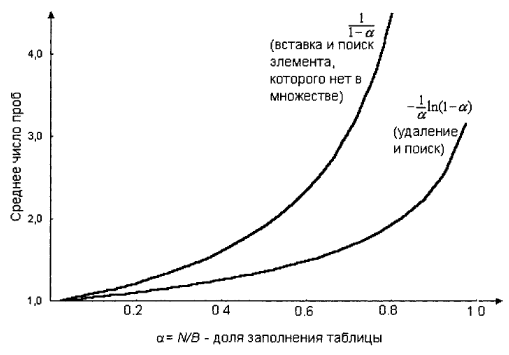
\includegraphics[scale = 1.0] {4,5.png}
		\caption*{Рис. 4.5. Средние числа проб, необходимые для выполнения операторов}
	\end{center}
\end{figure}

\subsection*{"Случайные" методики разрешения коллизий}
\addcontentsline{toc}{subsection}{ "Случайные" методики разрешения коллизий}
\normalsize
\indent

Мы ранее видели, что методика линейного повторного хеширования приводит к группированию заполненных сегментов в большие непрерывные блоки. Можно предложить хеш-функции с более "случайным"$\;$ поведением, например, ввести целочисленную константу $c$ > 1 и определить $h_i(x) = (h(x) + c_i)\; mod\;B$. В этом случае для $B$ = 8, $c$ = 3 и $h(x)$ = 4 получим "пробные" сегменты в следующем порядке: 4, 7, 2, 5, О, 3, 6 и 1. Конечно, если $B$ и $c$ имеют общие делители (отличные от единицы), то эта методика не позволит получить все номера сегментов, например при $B$ = 8 и $c$ = 2. Но более существенно, что даже если $B$ и $c$ \textit{взаимно простые числа} (т.е. не имеют общих делителей), то все равно существует проблема "группирования", как и при линейном хешировании, хотя здесь разделяются блоки заполненных сегментов, соответствующие различным константам $c$. Этот феномен увеличивает время выполнения операторов словарей (как и при линейном хешировании), поскольку попытка
вставить новый элемент в заполненный сегмент приводит к просмотру цепочки заполненных сегментов, различных для различных $c$, и длина этих цепочек при каждой вставке увеличивается на единицу.

Фактически любая методика повторного хеширования, где очередная проба \\зависит только от предыдущей (например, как зависимость от числа предыдущих
"неудачных" проб, от исходного значения $h(x)$ или от самого элемента $x$), обнаруживает группирующие свойства линейного хеширования. Возможна простейшая методика, для которой проблема "группирования" не существует: для этого достаточно положить $h_i(x) = (h(x) + d_i) \;mod\; B$, где $d_1, d_2, ..., d_{B - 1}$ - "случайные" перестановки чисел 1, 2, ..., $B - 1$. Конечно, такой набор чисел $d_1, d_2, ..., d_{B - 1}$ должен использоваться при реализации всех операторов, выполняемых над словарями, а "случайное" перемешивание целых чисел должно быть сделано (выбрано) еще при разработке алгоритма хеширования.

Генерация "хороших случайных" чисел - достаточно сложная задача, но, к счастью, существуют сравнительно простые методы получения последовательности "случайных" чисел путем "перемешивания" целых чисел из заданного интервала.


\noindent 
При наличии такого генератора случайных чисел можно воспроизводить требуемую последовательность $d_1, d_2, ..., d_{B - 1}$ при каждом выполнении операторов, работающих с хеш-таблицей.

Одним из эффективных методов "перемешивания"  целых чисел является метод
"последовательных сдвигов регистра"\rindex{Метод!последовательного сдвига регистра}. Пусть $B$ является степенью числа 2 и $k$ -  константа из интервала от 1 до $B - 1$. Начнем с некоторого числа $d_1$, взятого из интервала от 1 до $B - 1$. Далее генерируется последовательность чисел $d_i$ путем удвоения предыдущего значения до тех пор, пока последнее значение не превысит $B$. Тогда для получения следующего числа $d_i$ из последнего значения отнимается число $B$ и результат \textit{суммируется побитово по модулю 2 с константой $k$}. Сумма по модулю 2 \rindex{Сумма по модулю 2}чисел $x$ и $y$ (записывается как $x \oplus y$) определяется следующим образом: числа $x$ и $y$ записываются в двоичном виде с возможным приписыванием ведущих нулей так, чтобы числа имели одинаковую длину. Результат формируется по правилу логической операции "исключающего ИЛИ$"$, т.е. 1 в какой-либо позиции результата будет стоять тогда и только тогда, когда только в одной аналогичной позиции слагаемых стоит 1, но не в обеих.

\indent

Пример 4.7. $25 \oplus 13$ вычисляется следующим образом:
\begin{eqnarray}
25  & =   \;\;\;\;\;\;\:11001 \nonumber\\
13 & =  \;\;\;\;\;\;\:\underline{01101} \nonumber\\
25 \oplus 13 & =  10100 \nonumber
\end{eqnarray}

Отметим, что такое "суммирование" возможно с помощью обычного двоичного суммирования, если игнорировать перенос разрядов. 

Не для каждого значения $k$ можно получить все "перемешанные"$\;$ значения из 1,
2, ..., $B - 1$, иногда некоторые сгенерированные числа повторяются. Поэтому для
каждого значения В необходимо подобрать свое значение $k$, которое будет "работать".

Пример 4.8. Пусть $B$ = 8. Если мы положим $k$ = 3, то сгенерируем все числа от 0 до 7. Например, если начнем с числа $d_1$ = 5, то для нахождения следующего числа $d_2$ сначала удваиваем число $d_1$, получаем число 10, которое больше 8. Поэтому из 10 вычитаем 8, получаем 2 и вычисляем $d_2 = 2 \oplus 3 = 1$. Отметим, что для любого $x$ сумму $x \oplus 3$ можно вычислить путем инвертирования (преобразования в обратный код) последних двух двоичных разрядов числа $x$.

Повторяя описанную последовательность действий, получим числа $d_1, d_2, ..., d_7$ в виде 3-битовых двоичных чисел. Все этапы их вычисления показаны в табл. 4.2. Отметим, что умножение двоичного числа на 2 равнозначно сдвигу влево этого числа на один разряд - это оправдывает название "метод последовательного сдвига регистра".
\begin{onehalfspace}
\begin{table} [ht]
	\caption{Таблица 4.2. Вычисления по методу последовательного сдвига регистра}
	\begin{center}
		\begin{tabular}{c|c}
			& $d_1 = 101 = 5$ \\
			сдвиг& $1010$ \\
			удаление ведущей 1 (вычитание 8) & $010$ \\
			$\oplus 3$ & $d_2= 001 = 1$ \\
			сдвиг & $d_a = 010 = 2$ \\
			сдвиг & $d_4 = 100 = 4$ \\
			сдвиг & $100$ \\
			удаление ведущей 1 & $000$ \\
			$\oplus 3$ & $d_i = 011 = 3$ \\
			сдвиг & $d_6 = 110 = 6$ \\
			сдвиг & $1100$ \\
			удаление ведущей 1 & $100$ \\ 
			$\oplus 3$ & $d_7 = 111 = 7$ \\
		\end{tabular}
	\end{center}
\end{table}
\end{onehalfspace}
Читатель может проверить, что полный "перемешанный" набор чисел 1, 2, ..., 7
можно получить и для $k$ = 5, но ни при каких других значениях $d_i$.

\newpage

\subsection*{Рестуктуризация хэш-таблиц}
\addcontentsline{toc}{subsection}{ Рестуктуризация хэш-таблиц}
\normalsize
\indent

При использовании открытых хеш-таблиц среднее время выполнения операторов возрастает с ростом параметра $N/B$ и особенно быстро растет при превышении числа элементов над числом сегментов. Подобным образом среднее время выполнения операторов также возрастает с увеличением параметра $N/B$ и для закрытых хеш-таблиц, что видно из рис. 4.5 (но превышения $N$ над $B$ здесь невозможно).

Чтобы сохранить постоянное время выполнения операторов, которое теоретически возможно при использовании хеш-таблиц, мы предлагаем при достижении $N$ достаточно больших значений, например при $N > 0.9B$ для закрытых хеш-таблиц и $N > 2B$ - для открытых хеш-таблиц, просто создавать новую хеш-таблицу с удвоенным числом сегментов. Перезапись текущих элементов множества в новую хеш-таблицу в среднем займет меньше времени, чем их ранее выполненная вставка в старую хеш-таблицу меньшего размера. Кроме того, затраченное время на перезапись компенсируется более быстрым выполнением операторов словарей.

\section{Реализация АТД для отображений}
\normalsize
\indent

Вернемся к АТД MAPPING \rindex{MAPPING} (Отображение), введенным в главе 2, где мы определили отображение как функцию, ставящую в соответствие элементам области определения соответствующие элементы из области значений. Для этого АТД мы определили такие операторы.
\begin{enumerate}
	\item MAKENULL(A). Инициализирует отображение А,  где ни одному элементу области определения не соответствует ни один элемент области значений.
	\item ASSIGN(A, d, r). Задает для A(d) значение r.
	\item COMPUTE(A, d, r). Возвращает значение true и устанавливает значение г для
	A(d), если A(d) определено,-в противном случае возвращает значение false.
\end{enumerate}
\indent 

$\;\:$Отображения можно эффективно реализовать с помощью хеш-таблиц. Операторы ASSIGN и COMPUTE реализуются точно так же, как операторы INSERT и
MEMBER для словарей. Сначала рассмотрим применение открытых хеш-таблиц.
Предполагаем, что хеш-функция $h(x)$ распределяет элементы области определения по сегментам хеш-таблицы. Так же, как и для словарей, в данном случае сегменты содержат связанные списки, в ячейках которых находятся поля для элементов области определения и для соответствующих им элементов области значений. Для реализации такого подхода надо в листинге 4.8 заменить определение типа ячеек следующим объявлением:

\begin{lstlisting}[language=C,numbers=none]
    typedef struct  {
        |\textbf{domaintype}| mainelement;
        |\textbf{rangetype}| range;
        |\textbf{tcelltype}| next;
} celltype;
\end{lstlisting}

Здесь domaintype и rangetype - типы данных для элементов области определения
и области значений соответственно. Объявление АТД MAPPING следующее:

\begin{lstlisting}[language=C,numbers=none]
    typedef MAPPING celltype[B-1]
\end{lstlisting}


Последний массив - это массив сегментов для хеш-таблицы. Код процедуры\\
ASSIGN приведен в листинге 4.10. Написание процедур для операторов MAKENULL
и COMPUTE оставляем для упражнения.

\rindex{Реализация!операторов отображений}
\begin{lstlisting}[language=C, caption={Процедура ASSIGN для открытой хеш-таблицы}, numbers=none]
    void ASSIGN ( |\textbf{MAPPING}| *A, const |\textbf{domaintype}| *d,
                                        |\textbf{rangetype}| *r ) {
        int bucket;
        celltype current;

        bucket  = h(d);
        current = A[bucket];

        while (celltype != NULL)
            if (celltype->domainelement == d) {
                celltype->range  = r;
            /*|замена старого значения для $d$| */
                return;
            }
            else
                celltype = current->next; 
            /*|$d$ не найден в списке|*/

        celltype = A[bucket];
        /*|использование $Tcelltype$ для запоминания первой ячейки|*/
        new_celltype(A + bucket);
        A[bucket]->domainelement = d;
        A[bucket]->range = r;
        A[bucket]->next  = current;
    } /*|ASSIGN|*/
\end{lstlisting}

Подобным образом для реализации отображений можно использовать закрытое
хеширование. Ячейки хеш-таблицы будут содержать поля для элементов областей
определения и значений, а АТД MAPPING можно определить как массив таких
ячеек. Как и в случае открытого хеширования, хеш-функция применяется к элементам области определения, а не к элементам области значений. Мы оставляем читателю в качестве упражнения реализацию соответствующих операторов для закрытых хеш-таблиц.

\section{Очереди с приорететами}
\normalsize
\indent

Очередь с приоритетами - это АТД, основанный на модели множеств с операторами \rindex{Операторы!очереди с приоритетами} INSERT и DELETEMIN, а также с оператором MAKENULL для инициализации структуры данных. Перед определением нового оператора DELETEMIN\rindex{Оператор!DELETEMIN} сначала объясним, что такое "очередь с приоритетами". Этот термин подразумевает, что на множестве элементов задана функция приоритета (priority)\rindex{Функция!приоритета}, т.е. для каждого элемента а множества можно вычислить функцию $p(a)$, \textit{приоритет элемента а}, которая обычно принимает значения из множества действительных чисел, или, в более общем случае, из некоторого линейно упорядоченного множества. Оператор INSERT для очередей с приоритетами понимается в обычном смысле, тогда как DELETEMIN является функцией, которая возвращает элемент с наименьшим приоритетом и в качестве побочного эффекта удаляет его из множества. Таким образом, оправдывая свое название, DELETEMIN является комбинацией операторов DELETE и МIN, которые были описаны выше в этой главе.

Пример 4.9. Название "очередь с приоритетами" происходит от того вида упорядочивания (сортировки), которому подвергаются данные этого АТД. Слово "очередь" предполагает, что люди (или входные элементы) ожидают некоторого обслуживания,

\fancyfoot[LO]{4.10. ОЧЕРЕДИ С ПРИОРИТЕТАМИ}
\noindent  а слова "с приоритетом$"$ обозначают, что обслуживание будет производиться не по принципу "первый пришел - первым получил обслуживание", как происходит с АТД QUEUE \rindex{QUEUE} (Очередь), а на основе приоритетов всех персон, стоящих в очереди. Например, в приемном отделении больницы сначала принимают пациентов с потенциально фатальными диагнозами, независимо от того, как долго они или другие пациенты находились в очереди.

Более приемлемым для данной книги будет пример очереди с приоритетами, которая возникает среди множества процессов, ожидающих обслуживания совместноиспользуемыми ресурсами компьютерной системы. Обычно системные разработчики стараются сделать так, чтобы короткие процессы выполнялись незамедлительно (на практике "незамедлительно" может означать одну-две секунды), т.е. такие процессы получают более высокие приоритеты, чем процессы, которые требуют (или уже израсходовали) значительного количества системного времени. Процессы, которые требуют нескольких секунд машинного времени, не выполняются сразу - рациональная стратегия разделения ресурсов откладывает их до тех пор, пока не будут выполнены короткие процессы. Однако нельзя переусердствовать в применении этой стратегии, иначе процессы, требующие значительно больше времени, чем "средние$"$ процессы, вообще никогда не смогут получить кванта машинного времени и будут находиться в режиме ожидания вечно.

Один возможный путь удовлетворить короткие процессы и не заблокировать
большие состоит в задании процессу Р приоритета, который вычисляется по формуле 
$ 100_t{\text{исп}}(P) - t_{\text{исп}(P)} $.  Здесь параметр 
$ t_{\text{исп}} $ исп равен времени, израсходованному процессом $P$ ранее, a 
$ t_{\text{нач}} $ - время, прошедшее от начала инициализации процесса, отсчитываемое от некоего "нулевого времени". Отметим, что в общем случае приоритеты будут большими отрицательными целыми числами, если, конечно, 
$ t_{\text{нач}} $ не отсчитывается от "нулевого времени" в будущем. Число 100 в приведенной формуле является "магическим числом" (т.е. не поддается четкому логическому обоснованию, а пришедшему из практики) и должно быть несколько больше числа ожидаемых активных процессов. Читатель может легко увидеть, что если всегда сначала выполняется процесс с наименьшим приоритетным числом и если в очереди немного коротких процессов, то в течение некоторого (достаточно продолжительного) времени процессу, который не закончился за один квант машинного времени, будет выделено не менее 
1$\%$ машинного времени. Если этот процент надо увеличить или уменьшить, следует заменить константу 100 в формуле вычисления приоритета.

Представим процесс в виде записи, содержащей поле id идентификатора процесса
и поле \textit{priority} со значением приоритета, т.е. тип процесса processtype определим следующим образом:

\begin{lstlisting}[language=C,numbers=none]
    typedef struct {
        int id;
        int priority;
    }
\end{lstlisting}

Значение приоритета мы определили как целое число. Функцию определения приоритета (но не его вычисления) можно определить так:

\begin{lstlisting}[language=C,numbers=none]
    int р ( |\textbf{processtype}| a ) {
        return a.priority;
    }
\end{lstlisting}

Для того чтобы для выбранных процессов зарезервировать определенное количество квантов машинного времени, компьютерная система поддерживает очередь с приоритетом WAITING (Ожидание), состоящую из элементов типа processtype и использующую две процедуры: \textit{initial} (инициализация) и \textit{select}\rindex{Программа!select} (выбирать). Очередь WAITING управляется с помощью операторов INSERT и DELETEMIN.


\noindent При инициализации нового процесса вызывается процедура \textit{initial}, которая указывает записи, соответствующей новому процессу, место в очереди WAITING. Процедура \textit{select} вызывается тогда, когда система хочет "одарить$"$ квантом машинного времени какой-либо процесс. Запись для выбранного процесса удаляется из очереди WAITING, но сохраняется посредством \textit{select} для повторного ввода в очередь (если процесс не закончился за выделенное время) с новым приоритетом - приоритет 
увеличивается на 100 при пересчете времени $ t_{\text{исп}} $(когда $ t_{\text{исп}} $ увеличивается на единицу).

Можно использовать функцию \textit{currenttime} (которая возвращает текущее машинное время) для вычисления временных интервалов, отводимых системой
процессам; обычно эти интервалы измеряются в микросекундах. Будем также
использовать процедуру \textit{execute(P)} для вызова процесса с идентификатором $P$ на исполнение в течение одного кванта времени. В листинге 4.11 приведены коды процедур \textit{initial} и \textit{select}. $\square$

\rindex{Программа!выделения  процессам  машинного
времени}
\begin{lstlisting}[language=C, caption={Выделение процессам машинного времени}, numbers=none]
    /*|$initial$ указывает процессу с идентификатором $P$ место в очереди|*/
    void initial ( int Р) {
        |\textbf{processtype}| process;

        process->id = P;
        process->priority = -currenttime;
        INSERT(process, WAITING)
    } /*|initial|*/

    /*|select выделяет квант времени процессу с наивысшим приоритетом|*/
    void select(void) {
        |\textbf{processtype}| process;
        int begintime, endtime;

        process = DELETEMIN ( WAITING );
        /*|$DELETEMIN$ возвращает указатель на удаленный элемент|*/
        begintime = currenttime;
        execute (process->id);
        endtime = currenttime;
        process.priority = 
        process->priority + 100 * (endtime-begintime);
        /*|пересчет приоритета|*/
        INSERT (process, WAITING)
        /*|занесение процесса в очередь с новым приоритетом|*/
    } /*|select|*/

\end{lstlisting}

\section{Реализация очередей с приоритетами}\rindex{Реализация!операторов очереди с приоритетами}\rindex{Реализация!очередей с приоритетами}
\normalsize
\indent

За исключением хеш-таблиц, те реализации множеств, которые мы рассмотрели
ранее, можно применить к очередям с приоритетами. Хеш-таблицы следует исключить, поскольку они не имеют подходящего механизма нахождения минимального элемента. Попросту говоря, применение хеширования привносит дополнительные сложности, которых лишены, например, связанные списки.

При использовании связанных списков можно выбрать вид упорядочивания элементов списка или оставить его несортированным. Если список отсортирован, то нахождение минимального элемента просто - это первый элемент списка. Но вместе с тем вставка нового элемента в отсортированный список требует просмотра в среднем половины элементов списка. Если оставить список неупорядоченным, упрощается вставка нового элемента и затрудняется поиск минимального элемента.

\fancyfoot[LO]{4.11. РЕАЛИЗАЦИЯ ОЧЕРЕДЕЙ С ПРИОРИТЕТАМИ}


Пример 4.10. В листинге 4.12 показана реализация функции DELETEMIN для
несортированного списка элементов, имеющих тип processtype, описанный в примере 4.9. В этом листинге также приведены объявления для типа ячеек списка и для АТД PRIORITYQUEUE \rindex{PRIORITYQUEUE} \rindex{Абстрактный тип данных!PRIORITYQUEUE} (Очередь с приоритетами). Реализация операторов INSERT и MAKENULL (как для отсортированных, так и для несортированных списков) не вызывает затруднений, и мы оставляем ее в качестве упражнения для читателей. $\square$

\begin{lstlisting}[language=C, caption={Реализация очереди с приоритетами посредством связанного списка},numbers=none]
    typedef struct {
        |\textbf{processtype}| element;
        |\textbf{celltype}| next;
    } celltype;

    typedef PRIORITYQUEUE celltype;
    /*|ячейка указывает на заголовок списка|*/
    |\textbf{celltype}| DELETEMIN ( |\textbf{PRIORITYQUEUE}| *A ) {
        |\textbf{celltype}|  current;
        /*|указывает на ячейку, которая будет проверена следующей|*/
        int lowpriority;
        /*|содержит ранее найденный наименьший приоритет|*/
        |\textbf{celltype}| prewinner;
        /* |указывает на ячейку, содержащую элемент с наименьшим |
        |приоритетом|*/

        if (A->next == NULL)
            error("|Нельзя найти минимум в пустом списке|");
        else {
            lowpriority = p(AT->next->element);
            /* |функция $p$ возвращает приоритет первого элемента.|
            |Отметим, что $A$ указывает на ячейку заголовка, |
            |которая не содержит элемента.|*/
            prewinner = A;
            current   = At->next;
            while (current->next != NULL) {
                /*|сравнение текущего наименьшего приоритета с|
                |приоритетом следующего элемента|*/
                if (current->next->element 
                                < lowpriority) {
                    prewinner = current;
                    lowpriority = p(current->next->element);
                }
                current = current->next;
            }
            DELETEMIN = prewifiner->next;
            /*|возвращает указатель на найденный элемент|*/
            prewinner->next = prewinner->next->next;
            /*|удаляет найденный элемент из списка|*/
        }
    } /*|DELETEMIN|*/
\end{lstlisting}

\newpage

\subsection*{Реализация очереди с приоритетами посредством частично упорядоченных деревьев}
\addcontentsline{toc}{subsection}{ Реализация очереди с приоритетами посредством частично\\  упорядоченных деревьев}
\normalsize
\indent

Какие бы мы ни выбрали списки, упорядоченные или нет, для представления очередей с приоритетами придется затратить время, пропорциональное $n$, для выполнения операторов INSERT и DELETEMIN на множестве размера $n$. Существует другая реализация очередей с приоритетами, в которой на выполнение этих операторов требуется порядка  $O(\log{n})$ шагов, что значительно меньше $n$ для больших $n$ (скажем, для $n$ > 100). Основная идея такой реализации заключается в том, чтобы организовать элементы очереди в виде сбалансированного\footnote[1]{Сбалансированность в данном случае конструктивно можно определить так: листья возможны только на самом нижнем уровне или на предыдущем, но не на более высоких уровнях. Другими словами, максимально возможная сбалансированность двоичного дерева здесь понимается в том смысле, чтобы дерево было как можно "ближе" к полному двоичному дереву. Отметим также, что это понятие сбалансированности дерева не следует путать с а сбалансированностью деревьев и подобными характеристиками, хотя они и находятся в определенном "родстве". - Прим. ред.} (по возможности) двоич-
ного дерева (рис. 4.6). На нижнем уровне, где некоторые листья могут отсутствовать, мы требуем, чтобы все отсутствующие листья в принципе могли располагаться только справа от присутствующих листьев нижнего уровня.

Более существенно, что дерево \textit{частично упорядочено}\rindex{Дерево!частично упорядоченое}. Это означает, что приоритет узла $v$ не больше приоритета любого сына узла v, где приоритет узла - это значение приоритета элемента, хранящегося в данном узле. Из рис. 4.6 видно, что малые значения приоритетов не могут появиться на более высоком уровне, где есть большие значения приоритетов. Например, на третьем уровне располагаются приоритеты 6 и 8, которые меньше приоритета 9, расположенного на втором уровне. Но родитель узлов с приоритетами 6 и 8, расположенный на втором уровне, имеет (и должен иметь) по крайней мере не больший приоритет, чем его сыновья.

\begin{figure}[ht]
	\begin{center}
		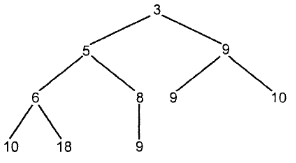
\includegraphics[scale = 1.2] {4,6.png}
		\caption*{Рис. 4.6. Частично упорядоченное дерево}
	\end{center}
\end{figure}

При выполнении функции DELETEMIN возвращается элемент с минимальным
приоритетом, который, очевидно; должен быть корнем дерева. Но если мы просто
удалим корень, то тем самым разрушим дерево. Чтобы не разрушить дерево и сохранить частичную упорядоченность значений приоритетов на дереве после удаления корня, мы делаем следующее: сначала находим на самом нижнем уровне самый правый узел и временно помещаем его в корень дерева. На рис. 4.7,а показаны изменения, сделанные на дереве рис. 4.6 после удаления корня. Затем этот элемент мы спускаем по ветвям дерева вниз (на более низкие уровни), по пути меняя его местами с сыновьями, имеющими меньший приоритет, до тех пор, пока этот элемент не станет листом или не встанет в позицию, где его сыновья будут иметь по крайней мере не меньший приоритет.

На рис. 4.7,а надо поменять местами корень и его сына, имеющего меньший приоритет, равный 5. Результат показан на рис. 4.7,6. Наш элемент надо спустить еще на более низкий уровень, так как его сыновья сейчас имеют приоритеты 6 и 8. 


\noindent  Меняем его местами с сыном, имеющим наименьший приоритет 6. Полученное в результате такого обмена новое дерево показано на рис. 4.7,в. Это дерево уже является частично упорядоченным и его дальше не надо менять.

\begin{figure}[ht]
	\centering
	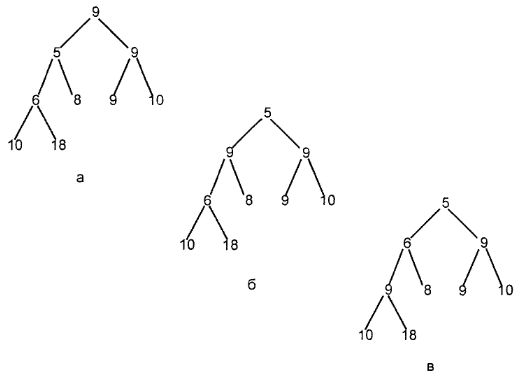
\includegraphics[scale = 1.1] {4,7.png}
	\caption*{Рис. 4.7. Спуск элемента по дереву}
\end{figure}

Если при таком преобразовании узел $v$ содержит элемент с приоритетом $a$ и его сыновьями являются элементы с приоритетами $b$ и $c$, из которых хотя бы один меньше а, то меняются местами элемент с приоритетом $a$ и элемент с наименьшим приоритетом из $b$ и $c$. В результате в узле $v$ будет находиться элемент с приоритетом, не превышающим приоритеты своих сыновей. Чтобы доказать это, для определенности положим, что $b \le c$ . После обмена элементами узел $v$ будет содержать элемент c приоритетом $b$, а его сыновья - элементы с приоритетами $a$ и $c$. Мы предположили, что $b < c$ и $a$ не меньше, по крайней мере, или $b$, или $c$. Отсюда следует $b < a$, что и
требовалось доказать. Таким образом, описанный процесс спуска элемента по дереву приводит к частичному упорядочиванию двоичного дерева.

Теперь покажем, что оператор DELETEMIN, выполняемый над множеством из $n$
элементов, требует времени порядка $O(\log{n})$. Это следует из того факта, что в дереве нет пути, состоящего из больше чем $1 + \log{n}$ узлов\footnote[1]{Здесь подразумевается логарифм по основанию 2. Приведенную оценку можно доказать
	исходя из упражнения 3.18 главы 3 или непосредственно методом математической индукции по $n$. — Прим. ред.}, а также вследствие того, что процесс прохождения элементом каждого узла занимает постоянное фиксированное время. Так как для любой положительной константы $c$ и при $n > 2$ величина $c(1 +  \log{n})$ не превышает $2c\log{n}$, то $c(1 + \log{n})$ имеет порядок $O(\log{n})$.

Теперь рассмотрим, как на частично упорядоченных деревьях работает оператор
INSERT. Сначала поместим новый элемент в самую левую свободную позицию на самом нижнем уровне, если же этот уровень заполнен, то следует начать новый уровень.


\newpage

\noindent На рис. 4.8,а показана вставка элемента с приоритетом 4 в дерево из рис. 4.6. Если новый элемент имеет меньший приоритет, чем у его родителя, то они меняются местами. Таким образом, новый элемент теперь находится в позиции, когда у его сыновей больший приоритет, чем у него. Но возможно, что у его нового родителя приоритет больше, чем у него. В этом случае они также меняются местами. Этот процесс продолжается до тех пор, пока новый элемент не окажется в корне дерева или не займет позицию, где приоритет родителя не будет превышать приоритет нового элемента. Рис. 4.8,б, в показывают этапы перемещения нового элемента.

\begin{figure}[ht]
	\centering
	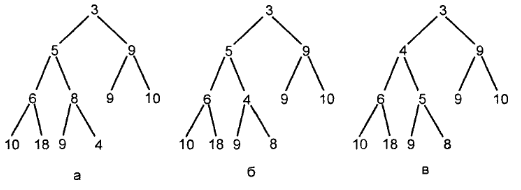
\includegraphics[scale = 1.1] {4,8.png}
	\caption*{Рис. 4.8. Вставка нового элемента}
\end{figure}

Теперь докажем, что в результате описанных выше действий получим частично
упорядоченное дерево. Поскольку мы не пытаемся провести строгое доказательство, то просто рассмотрим ситуации, когда элемент с приоритетом $a$ может стать родителем элемента с приоритетом $b$. (Далее для простоты изложения будем отождествлять элемент с его приоритетом.)

\begin{enumerate}
	\item  Элемент $a$ - это новый элемент, который, перемещаясь по дереву вверх, заменил родителя элемента $b$. Пусть старый родитель элемента $b$ имел приоритет $c$, тогда $a < c$, иначе не произошла бы замена. Но $c < b$, поскольку исходное дерево частично упорядочено. Отсюда следует, что $a < b$. Пример такой ситуации показан на рис. 4.8,в, где элемент 4 становится родителем элемента 6, заменяя его родителя с приоритетом 5.
	\item  Элемент $a$ спустился вниз по дереву вследствие обмена с новым элементом. В этом случае в исходном дереве элемент $a$ должен быть предком элемента $b$. Поэтому $a < b$. На рис. 4.8,в элемент 5, ставший родителем элементов с приоритетами 8 и 9, ранее был их "дедушкой".
	\item  Элемент $b$ - новый элемент, который, перемещаясь вверх по дереву, стал сыном элемента $a$. Если $a > b$, то на следующем шаге они поменяются местами, ликвидируя тем самым нарушение свойства упорядоченности дерева.
\end{enumerate}
\indent 

Время выполнения оператора вставки пропорционально пути, пройденному новым элементом. Так же, как и в случае оператора DELETEMIN, этот путь не может быть больше $1+ \log{n}$. Таким образом, время выполнения обоих этих операторов имеет порядок $O(\log{n})$.

\subsection*{Реализация частично упорядоченных деревьев посредством\\ массивов}\rindex{Реализация!частично упорядоченных деревьев посредством массивов} %%snes \\
\addcontentsline{toc}{subsection}{ Реализация частично упорядоченных деревьев посредством массивов}
\normalsize
\indent

Исходя из того, что рассматриваемые нами деревья являются двоичными, по возможности сбалансированными и на самом нижнем уровне все листья "сдвинуты"  влево, можно применить для этих деревьев необычное представление, которое называется \textit{куча}\rindex{Куча}. В этом представлении используется массив, назовем его $A$, в котором первые $n$ позиций соответствуют $A$ узлам дерева. $A[1]$  содержит корень дерева. Левый
сын узла $A[i]$, если он существует, находится в ячейке $A[2i]$, а правый сын, 


\noindent если он также существует, - в ячейке $A[2i + 1]$. Обратное преобразование: если сын находится в ячейке $A[i], i > 1$, то его родитель - в ячейке $A[i\; div \;2]$. Отсюда видно, что узлы дерева заполняют ячейки $A[1], A[2], ..., A[n]$ последовательно уровень за уровнем, начиная с корня, а внутри уровня - слева направо. Например, дерево, показанное на рис. 4.6, будет представлено в массиве следующей последовательностьюсвоих узлов: 3, 5, 9, 6, 8, 9, 10, 10, 18, 9.

В данном случае мы можем объявить АТД PRIORITYQUEUE\rindex{PRIORITYQUEUE!объявление} (Очередь с \\приоритетами) как записи с полем \textit{contents} для массива элементов типа, например processtype, как в примере 4.9, и полем \textit{last} целочисленного типа, значение которого указывает на последний используемый элемент массива. Если мы также введем константу \textit{maxsize}, равную количеству элементов очереди, то получим следующее объявление типов:

\begin{lstlisting}[language=C,numbers=none]
    typedef struct {
        |\textbf{processtype}| contents[maxsize];
        int last;
    } PRIORITYQUEUE;
\end{lstlisting}

Реализация операторов,  выполняемых над очередью с приоритетами,  показана в
следующем листинге.

\begin{lstlisting}[language=C, caption={Реализация очереди с приоритетами посредством массива}, numbers=none]
    void MAKENULL ( |\textbf{PRIORITYQUEUE}| *A ) {
        A->last = 0;
    }; #|MAKENULL|

    void INSERT ( const |\textbf{processtype}| *x, |\textbf{PRIORITYQUEUE}| *A ) {
        int i;
        |\textbf{processtype}| temp;

        if ( A->last >= maxsize)
            error("|Очередь заполнена|");
        else {
            A->last = A->last + 1;
            A->contents[A->last] = x;
            i = A->last; #|i - индекс текущей позиции х|
            while ((i > 1) && 
                    (p(A->contents[i]) < 
                            p(A->contents[i div 2])))
            { /*|перемещение x вверх по дереву путем|
                | обмена местами с родителем,| 
                |имеющим больший приоритет|*/
                temp = A->contents[i];
                |Л|->contents[i] = A->contents[i div 2];
                A->contents[i div 2] = temp;
                i = i div 2;
            }
        }
    } #|INSERT|

    |\textbf{processtype}| DELETEMIN ( |\textbf{PRIORITYQUEUE}| *A ) {
        int i, j;
        |\textbf{processtype}| temp;
        |\textbf{processtype}| minimum;

        if ( A->last == 0)
            error("|Очередь пуста|");
        else {
            new_pocesstype(&minimum);
            minimum = A->contents[0];
            A->contents[0] = A->contents[A->last];
            A->last = A->last - 1;
            i = 1;
            while (i <= A->last div 2) {
                /*|перемещение старого последнего элемента|
                        |вниз по дереву|*/
                if ((p(A->contents[2*i]) < 
                        p(А->contents[2*i+1]))or(2*i == A->last))
                    j = 2 * i;
                else
                    j = 2 * i + 1;
            /*|j будет сыном i с наименьшим приоритетом или,|
                |если 2*i == A->last, будет просто сыном i |*/
                if ( р(А->contents[i]) > 
                        р(А->contents[j])) {
            /*|обмен старого последнего элемента с |
                |сыном, имеющим наименьший| 
                            |приоритет|*/
                    temp = A->contents[i];
                    A->contents[i] = A->contents[j];
                    A->contents[j] = temp;
                    i = j;
                }
                else
                    return minimum;
                #|дальше перемещение элемента невозможно|
            }
            return(minimum); #|элемент дошел до листа|
        }
    } #|DELETEMIN|
\end{lstlisting}

\fancyfoot[LO]{4.12. НЕКОТОРЫЕ СТРУКТУРЫ СЛОЖНЫХ МНОЖЕСТВ}


\section{Некоторые структуры сложных множеств}
\normalsize
\indent

В этом разделе мы рассмотрим применение двух сложных множеств для пред-
ставления данных. В первом примере рассмотрим представление отношений "многие-ко-многим", которые встречаются в системах баз данных. Далее мы изучим, как с помощью двух структур данных можно представить какой-либо объект (в нашем случае - отображение) более эффективно, чем при представлении этого объекта одной структурой.

\subsection*{Отношения "многие-ко-многим" и структура мультисписков}\rindex{Мультисписки}
\addcontentsline{toc}{subsection}{ Отношения "многие-ко-многим" и структура мультисписков}
\normalsize
\indent

Пример отношения "многие-ко-многим" между множеством студентов и множеством учебных курсов (учебных предметов) показан в табл. 4.3. Отношение "многие-ко-многим" называется так потому, что на каждый курс могут записаться много студентов (не один) и каждый студент может записаться на несколько курсов.

Время от времени может возникнуть необходимость вставить или удалить студентов с какого-либо курса, определить, какие студенты посещают тот или ной курс, или узнать, какие курсы посещает конкретный студент. Простейшей структурой данных, 


\noindent которая удовлетворяет этим запросам, является двумерный массив, подобный табл. 4.3, где значение 1 (или true) соответствует значку "X$"$, а значение О (или false) - пробелу.
\begin{onehalfspace}
\begin{table}[ht]
	\caption{ Пример отношения между множеством студентов и множеством учебных курсов}
	\begin{center}
		\begin{tabular}{lccc}
			& \text{$\;\;\;\;\;$} CS101\text{$\;\;\;\;\;$} & \text{$\;\;\;\;\;$} CS202\text{$\;\;\;\;\;$} & CS303 \\ 
			\\[-1em] \cline{2-4} 
			& \multicolumn{1}{|c|}{}  & \multicolumn{1}{c|}{}  & \multicolumn{1}{c|}{} \\[-0.8em]
			Alan    & \multicolumn{1}{|c|}{}  & \multicolumn{1}{c|}{}  & \multicolumn{1}{c|}{X} \\	
			Alex    & \multicolumn{1}{|c|}{X} & \multicolumn{1}{c|}{X} & \multicolumn{1}{c|}{}  \\
			Alice    & \multicolumn{1}{|c|}{}  & \multicolumn{1}{c|}{}  & \multicolumn{1}{c|}{X} \\
			Amy     & \multicolumn{1}{|c|}{X} & \multicolumn{1}{c|}{}  & \multicolumn{1}{c|}{}  \\
			Andy    & \multicolumn{1}{|c|}{}  & \multicolumn{1}{c|}{X} & \multicolumn{1}{c|}{X} \\
			Ann    & \multicolumn{1}{|c|}{X} & \multicolumn{1}{c|}{}  & \multicolumn{1}{c|}{X} \\ \cline{2-4} 
			\\[-0.8em]
			& \multicolumn{3}{c}{\textit{Регистрация (студентов по учебным курсам)}}  
		\end{tabular}
	\end{center}
\end{table}
\end{onehalfspace}

Чтобы приписать студента к какому-либо курсу, надо использовать отображение (назовем его MS), которое можно реализовать как хеш-таблицу, для преобразования имени студента в индекс массива, а также еще одно отображение \textit{МС}, переводящее название курса в другой индекс массива. Тогда запись студента $s$ на курс $c$ можно представить в виде простого присваивания элементу массива $Enrollment$ (Регистрация) значения 1:

\[
Enrollment[MS(s),MC(c)] = 1;
\]

Открепление студента с курса выполняется путем задания значения О соответствующему элементу массива \textit{Enrollment}. Для определения курсов, которые посещает студент с именем $s$, надо просмотреть строку 
$MS(s)$, а для получения списка студентов, посещающих курс с, надо просмотреть столбец $MC(c)$.

Почему для представления подобных данных надо использовать другую, более подходящую структуру данных? Представим большой университет, где учатся примерно 20 000 студентов и изучается не менее 1 000 учебных курсов, при этом каждый студент одновременно изучает в среднем только три учебных курса. Тогда при использовании массива, подобного табл. 4.3, этот массив будет состоять из 20 000 000 элементов, из которых только 60 000, или примерно 0.3$\%$, будут иметь значение 1\footnote[1]{ Если бы это была реальная база данных, то такой массив должен храниться на устройстве
	внешней памяти. Но такая структура данных слишком расточительна даже для внешней памяти.}. Такой массив называют \textit{разреженным}, так как большинство его элементов имеют нулевые значения. Можно сберечь значительный объем памяти, если хранить не весь разреженный массив, а только его ненулевые элементы. Более того, в этом случае можно значительно сократить время просмотра этого массива. Например, вместо просмотра столбца из 20 000 элементов надо просмотреть в среднем всего
60 элементов. Просмотр элементов по строкам займет примерно такое же время.

Еще один подход к решению исходной задачи состоит в ее переформулировке: вместо представления данных, подобных табл. 4.3, в виде одного множества можно создать систему поддержки набора множеств и отношений между ними. В нашем случае очевидны два множества: имен студентов S и названий учебных курсов С. Каждый элемент множества S будет иметь тип studenttype (тип студента), который можно представить в виде записей следующего типа:

\begin{lstlisting}[language=C,numbers=none]
    typedef struct {
        int id;
        char name[30];
    } STUDENTTYPE;
\end{lstlisting}


\newpage

Подобное определение можно сделать для элементов множества $C$. Для реализации отношений между элементами множеств необходимо третье множество $E$, каждый элемент которого должен соответствовать одной ячейке массива регистрации, где есть знак "X$"$ (см. табл. 4.3). Элементы множества $E$ должны быть записями фиксированного типа. Мы пока не можем сказать, какие поля должны содержать эти записи\footnote[1]{На практике в записях, подобных регистрационным, удобно иметь поля типа метки или статуса, но наша исходная задача этого не требует.}, но далее
мы рассмотрим несколько возможных вариантов таких полей. Сейчас мы просто постулируем, что есть регистрационные записи для каждой ячейки массива, помеченной знаком "X$"$, и эти записи каким-то образом отделены одна от другой.

Нам также нужны множества, соответствующие ответам на основные вопросы: какие учебные курсы посещает конкретный студент $s$ (это множество обозначим $C_s$) и какие студенты записаны на данный курс $c$ (это множество $S_c$). Реализации этих множеств вызывают затруднения, поскольку заранее нельзя сказать, сколько будет элементов в этих множествах, что, в свою очередь, принуждает усложнять записи, касающиеся студентов и курсов. Можно сделать множества $C_s$ и $S_c$ не множествами
непосредственно записей, а множествами указателей на студенческие и курсовые записи. В этом случае экономится значительная часть пространства памяти и можно быстро получить ответы на сформулированные выше вопросы.

Пока пусть каждое множество $C_s$ является множеством регистрационных записей, 
соответствующих конкретному студенту $s$ 
и некоторому учебному курсу $c$. 
Если принять за регистрацию пару $(s, c)$, 
то множество $ C_s $ можно определить следующим образом:

\[
C_s - \{(s, c) | \text{студент}\; s \;\text{записан на курс}\; c\}.
\]

Аналогично определяется множество $S_c$:
\[
S_c - \{(s, c) | \text{студент}\; s \;\text{записан на курс}\; c\}.
\]

Отметим различие в определении этих множеств: в первом множестве $s$ является\\ константой, а во втором - $c$. 
Например, основываясь на табл. 4.3, \\$C_{Alex} = \{(Alex, CS101), (Alex, CS202)\}$ и \\$S_{CS101} = \{(Alex, CS101), (Amy, CS101), (Ann, CS101)\}$.

\subsection*{Структуры мультисписков}
\addcontentsline{toc}{subsection}{ Структуры мультисписков}

В общем случае структура мультисписка - это совокупность ячеек, некоторые из которых имеют более одного указателя и поэтому одновременно могут принадлежать нескольким спискам. Для каждого типа ячеек важно различать пбля указателей для разных списков, чтобы можно было проследить элементы одного списка, не вступая в противоречие с указателями другого списка.

С этой точки зрения можно задать поля указателя в каждой записи для студента и для курса, которые указывали бы на первые регистрационные записи множеств $C_s$, и $S_c$ соответственно. Каждая регистрационная запись должна иметь два поля указателя, одно из них, назовем его \textit{cnext}, будет указывать на следующую регистрационную запись списка множества $C_s$, которому она принадлежит, а второе поле, \textit{snext}, будет указывать на следующую регистрационную запись списка множества $S_c$,  которому она также принадлежит.

Оказывается, что при таком задании полей указателей в регистрационных записях они могут не указывать непосредственно ни на студента, ни на курс, которым она (регистрационная запись) соответствует. Эта информация неявно содержится в списках, которым принадлежит регистрационная запись. Назовем студенческие и курсовые записи, возглавляющие такие списки, \textit{собственниками} регистрационной записи. Таким образом, чтобы найти те курсы, которые посещает студент $s$, надо просмотреть все регистрационные записи из $C_s$, и для каждой из них найти собственника среди курсовых записей. Для этого достаточно поместить в каждую регистрационную запись указатели на обоих собственников.

\newpage

Благодаря таким указателям можно получить ответы на интересующие нас вопросы за минимально возможное время. Но можно значительно сократить объем памяти, занимаемой такой структурой\footnote[1]{Отметим, что, как правило, регистрационных записей значительно больше, чем записей о студентах и учебных курсах, поэтому, даже незначительно сокращая пространство, занимаемое одной регистрационной записью, мы существенно сокращаем общее требуемое пространство памяти.}, если исключить описанные выше указатели на собственников из регистрационных записей, оставив их только в конечных записях списков каждого $C_s$ и $S_c$.  
Таким образом, каждая запись о студенте или курсе становится частью кольца, включающего все регистрационные записи, для которых данная запись о студенте или курсе является собственником. Такие кольца можно видеть на рис. 4.9 для данных из табл. 4.3. Отметим, что. на этом рисунке регистрационные записи состоят из поля \textit{cnext} (левое) и поля \textit{snext} (правое).


\begin{figure}[ht]
	\centering
	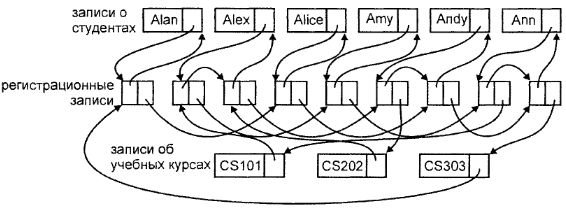
\includegraphics[scale = 1.0] {4,9.png}
	\caption*{Рис. 4.9. Представление данных из табл. 4.3 посредством мультисписка}
\end{figure}

Пример 4.11. Для ответа на вопрос, какие студенты зарегистрированы на курсе CS101, сначала находим запись для этого учебного курса. Как найти эту запись, зависит от организации множества курсов. Например, это может быть хеш-таблица, содержащая все курсовые записи, тогда определить нужную запись можно посредством хеш-функции, примененной к "CS101".

Далее следуем за указателем из записи курса CS101 на первую регистрационную запись кольца для этого курса. На рис. 4.9 это вторая слева регистрационная запись. Теперь надо найти собственника-запись студента, которому принадлежит данная регистрационная запись. Для этого мы следуем за указателями /textit{cnext} (первый указатель в регистрационной записи), пока не достигнем указателя на запись студента\footnote[2]{Чтобы отличить указатель на регистрационную запись от указателя на запись студента, надо как-то определять тип записей. Этот вопрос мы рассмотрим немного ниже.}. В данном случае мы остановимся на третьей регистрационной записи, которая указывает на запись студента Alex. Таким образом, мы узнали, что Alex посещает учебный курс CS101.

Теперь надо найти следующего студента, посещающего курс CS101. Для этого надо следовать за указателем \textit{snext} (второй указатель в регистрационной записи), начиная со второй регистрационной записи. В данном случае он приведет к пятой регистрационной записи. В этой записи указатель cnext непосредственно указывает на собственника-запись студента, которая соответствует студенту Amy. Таким образом, студент Amy также посещает курс CS101. Следуя далее за указателем \textit{snext} пятой
регистрационной записи, мы перейдем к восьмой регистрационной записи. Кольцо указателей cnext приведет от этой записи к девятой регистрационной записи, собственником которой является запись, соответствующая студентке Ann, также посещающей курс CS101. Указатель \textit{snext} восьмой регистрационной записи возвращает нас на запись курса CS101. Это означает, что множество $S_c$ исчерпано. $\square$



В обобщенном виде операторы, реализующие действия, описанные в примере 4.11, можно записать следующим образом:

\noindent for для каждой записи регистрации из множества $S_c$ курса CS101 

\begin{lstlisting}[language=C,numbers=none]
    s = |студент-собственник регистрационной записи|;
    print(s); 
\end{lstlisting}

Здесь оператор присваивания можно детализировать так:

\begin{lstlisting}[language=C,numbers=none]
    f = е;
    do {
        f = f->cnext;
    } while (|$f$ - указатель на запись студента|);
        s = |значению поля $studentname$ в записи, на которую указывает $f$|;
\end{lstlisting}

где $e$- указатель на первую регистрационную запись в множестве $S_c$ курса CS101.

Для реализации структуры, подобной показанной на рис. 4.9, на языке $C$ необходим только тип record (запись) в различных вариантах для записей, относящихся к именам студентов, названиям курсов и регистрации. Но возникают трудности, связанные с тем, что указатели полей \textit{cnext} и \textit{snext} могут указывать записи разных типов. Эти трудности можно обойти, если определять тип записи циклически. В листинге 4.14 показаны такие объявления типов, а также процедура \textit{printstudents} вывода на печать имен студентов, посещающих определенный учебный курс.

\begin{lstlisting}[language=C, caption={Реализация поиска в мультисписке\rindex{Поиск!в мультисписке}}, numbers=none]
    typedef char[20] stype;
    typedef char[5] ctype;

    typedef enum {
        student,
        course,
        enrollment
    } recordkinds;

    typedef struct _rc {
        |\textbf{recorkinds}| kind;
    
        union {
            struct {
                |\textbf{stype}| studentname;
                struct _rc *firstcourse;
            } s_student;

            struct {
                |\textbf{ctype}| coursename;
                struct _rc *firststudent;
            } s_course;

            struct {
                struct _rc *cnext;
                struct _rc *snext;
            } s_enrollment;
        } val;
    } recordtype;

    void printstudents (|\textbf{ctype}| cname) {
        |\textbf{recordtype}| *c, *e, *f;
        c  = |указатель на запись курса, где c->coursename == cname|;
            /*|последний оператор зависит от того,|
            |как реализовано множество записей курсов|*/
        е = c->val.s_course.firststudent;
        /* |е пробегает по кольцу указателей|
            |регистрационных записей|*/
        while (e->kind == enrollment) {
            f = e;
            do {
                f = f->val.s_enrollement.cnext;
            }while (f->kind != student);
        /*|сейчас $f$ - указатель на студента-собственника регистрации $e$|*/
            printf("\%s\n", f->val.s_student.studentname);
            e = e->val.s_enrollement.snext;
    } #|printstudents|

\end{lstlisting}

\subsection*{Эффективность двойных структур данных}\rindex{Структуры данных!двойные}
\addcontentsline{toc}{subsection}{ Эффективность двойных структур данных}
\normalsize
\indent

Часто кажущаяся простота представления множеств или отображений на самом деле оборачивается трудной проблемой выбора подходящей структуры данных. \\
Какая-либо структура данных, представляющая множество, позволяет легко выполнять определенные операторы, но на выполнение других приходится затрачивать значительное время. По-видимому, не существует одной структуры данных, позволяющей всем операторам выполняться быстро и просто. 
В этом случае решением может стать использование двух или больше структур данных для представления одного и того же множества или отображения.

Предположим, что мы хотим создать "теннисную лестницу" (т.е. квалификационную таблицу), где каждый игрок располагается на своей "ступеньке" (рейтинге). Новые игроки добавляются в самый низ, т.е. на ступеньку с самым большим номером. Игрок может вызвать на поединок игрока, стоящего на более высокой ступени, и если он выиграет матч, то они меняются ступенями. Эту "лестницу" можно рассматривать как абстрактный тип данных \rindex{Абстрактный тип данных}, где базовой моделью будет отображение из множества имен игроков (строки символов) в множество номеров ступеней (целые числа 1, 2, ...). Необходимы также три оператора, выполняемые над этим АТД.

\begin{enumerate}
	\item  АDD(имя) добавляет новое имя в квалификационную лестницу на свободную ступеньку с наибольшим номером, т.е. в самый низ лестницы.
	\item  CHALLENGE(имя) возвращает имя игрока, стоящего на ступени $i - 1$, если игрок имя стоит на ступени $i, i > 1$.
	\item  EXCHANGE(i)\footnote[1]{Названия операторов переводятся соответственно как "Добавить", "Вызов" (на поединок)
		и "Обмен". — Прим. перев.} меняет местами игроков, стоящих на ступенях $i$ и$\;i - 1, i > 1$.
\end{enumerate}
\indent

Для реализации описанных данных и их операторов можно использовать массив \textit{LADDER} (Лестница), где $LADDER[i]$ - имя игрока, стоящего на ступени $i$. Вместе с именем игрока можно хранить и его номер (т.е. номер ступени, на которой он стоит). В этом случае нового игрока можно просто добавить за малое фиксированное время в свободную ячейку массива.

Оператор EXCHANGE реализуется легко - меняются местами два элемента массива. Но выполнение функции CHALLENGE в процессе поиска заданного имени требует времени порядка $O(n)$ для просмотра всего массива (здесь и далее и - общее число игроков).

С другой стороны, мы можем применить хеш-таблицу для задания отображения из множества имен в множество номеров ступеней. Количество сегментов в хеш-таблице примерно равно количеству игроков. Оператор ADD выполняется в среднем за время $O(1)$. Функция CHALLENGE тратит в среднем $O(1)$ времени на поиск заданного имени, но требует $O(n)$ времени для поиска имени соперника, стоящего на более высокой ступени,
поскольку в этом случае надо просмотреть всю хеш-таблицу. Оператор EXCHANGE требует $O(n)$ времени для поиска имен игроков, стоящих на ступенях $i$ и $i - 1$.

Теперь рассмотрим применение комбинации двух структур. Пусть ячейки хеш-
таблицы содержат имя игрока и его номер ступени, а в массиве \textit{LADDER} элемент $LADDER[i]$ будет указателем на ячейку игрока в хеш-таблице, стоящего на $i$-й ступени, как показано на рис. 4.10.

\begin{figure}[ht]
	\centering
	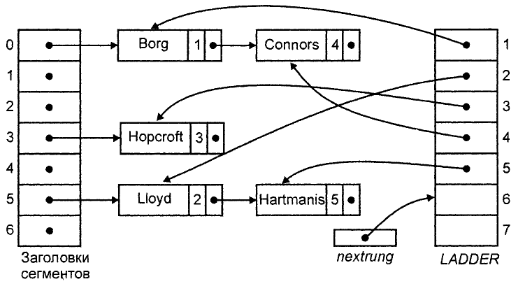
\includegraphics[scale = 1.1] {4,10.png}
	\caption*{Рис. 4.10. Комбинированная структура высокой производительности}
\end{figure}

При такой организации данных добавление нового игрока требует в среднем \\$O(1)$ времени 
для записи его атрибутов в хеш-таблицу, а также создания указателя на его ячейку в хеш-таблице из ячейки массива \textit{LADDER}, которая помечена курсором \textit{nextrung} (следующая ступень) (см. рис. 4.10). 
При выполнении функции CHALLENGE надо сначала найти заданное имя в хеш-таблице (на это требуется в среднем $O(1)$ времени), получить его номер ступени i и далее, следуя за указателем из ячейки $LADDER[i - 1]$ в ячейку хеш-таблицы, получить имя игрока-соперника. 
Все последние описанные действия в среднем требуют не более $O(1)$ времени, поэтому
все время выполнения функции CHALLENGE имеет в среднем порядок $O(1)$.

Оператор EXCHANGE($i$) требует времени порядка $O(1)$ для нахождения имен игроков с рангами $i$ и $i - 1$, для обмена содержимым двух ячеек хеш-таблицы и обмена указателями в двух ячейках массива \textit{LADDER}. 
Таким образом, даже в самом худшем случае время выполнения оператора EXCHANGE не будет превышать некоторой фиксированной величины.


\subsection*{Упражнения}
\addcontentsline{toc}{subsection}{ Упражнения}

\begin{enumerate}
	\item[4.1.] Пусть заданы два множества А — $\{$1, 2, 3$\}$ и В = $\{$3, 4, 5$\}$. Каков будет результат выполнения следующих операторов?
	\begin{enumerate}
		\item[a)] UNION($A, B, C$);
		\item[б)] INTERSECTION($A, B, C$);
		\item[в)] DIFFERENCES($A, B, C$);
		\item[r)] MEMBER(1, $A$);
		\item[д)] INSERT(1, $A$);
		\item[e)]DELETE(1, $A$);
		\item[ж)] МIN($A$).
	\end{enumerate}
	\item[*4.2.] Напишите процедуру в терминах базовых операторов множеств для печати всех элементов произвольного конечного множества. Предполагается, что элементы множества имеют тип, допустимый для печати. Процедура печати не должна разрушать исходное множество. Какова в данном случае наиболее подходящая структура данных для реализации множества?
	

	
	\item[4.3.] Реализацию множеств посредством двоичных векторов можно использовать тогда, когда "универсальное множество" $\;$ преобразовано в последовательность целых чисел от 1 до $N$. Опишите такое преобразование для следующих универсальных множеств:
	\begin{enumerate}
		\item[a)] множество целых чисел 0, 1, ..., 90;
		\item[б)] множество целых чисел от $n$ до $m$, где $a$ < 0;
		\item[в)] множество целых чисел $n, n+2, n+4, ..., a + 2k $ для любых $n$ и $k$;
		\item[r)] множество символов 'а', 'b', ..., V;
		\item[д)] массив двухсимвольных строк, каждый символ может быть любым симво-
		лом из множества 'а', 'b', ..., V.
	\end{enumerate}
	\item[4.4.] Напишите процедуры MAKENULL, UNION, INTERSECTION, MEMBER, MIN, INSERT и DELETE для множеств, представленных посредством списков, используя обобщенные операторы АТД сортированных списков. Отметим, что в листинге 4.3 используется специфическая реализация АТД списков.
	\item[4.5.] Повторите упражнение 4.4 для следующих реализаций множеств:
	\begin{enumerate}
		\item[а)] открытая хеш-таблица (используйте обобщенные операторы списков, работающие с сегментами);
		\item[б)] закрытая хеш-таблица с линейной методикой разрешения коллизий;
		\item[в)] несортированный список (используйте обобщенные операторы списков);
		\item[г)] массив фиксированной длины и указатель на последнюю занятую позициюв массиве.
	\end{enumerate}
	\item[4.6.] Для каждой реализации и каждого оператора из упражнений 4.4 и 4.5 найдите порядок времени выполнения операторов над множествами размера $n$.
	\item[4.7.] Предположим, что для хеширования целых чисел в 7-сегментную хеш-таблицу используется хеш-функция $h(i) = i\; mod \;7$.
	\begin{enumerate}
		\item[а)] приведите результирующую хеш-таблицу, если в нее вставляются точные кубы 1, 8, 27, 64, 125, 216, 343;
		\item[б)] повторите предыдущий пункт для закрытой хеш-таблицы с линейной методикой разрешения коллизий.
	\end{enumerate}
	\item[4.8.] Предположим, что есть закрытая хеш-таблица с 5 сегментами, хеш-функцией $A(i) = i\; mod\; 5$ и линейной методикой разрешения коллизий. Покажите результат вставки в первоначально пустую хеш-таблицу последовательности чисел 23, 48, 35, 4, 10.
	\item[4.9.] Приведите реализацию операторов АТД отображений с использованием открытой и закрытой хеш-таблиц.
	\item[4.10.] Чтобы увеличить скорость выполнения операторов, мы хотим заменить открытую хеш-таблицу с $B_1$ сегментами, содержащую значительно больше чем $B_1$ элементов, на другую хеш-таблицу с $B_2$ сегментами. Напишите процедуру преобразования старой хеш-таблицы в новую, используя операторы АТД списков для заполнения каждого сегмента.
	\item[4.11.] В разделе 4.8 мы обсуждали "случайные" хеш-функции, когда для проверки сегментов после возникновения $i$-й коллизии применяется функция $h_i(x) = (h(x) + d_i)\; mod \;B$ с использованием некоторой последовательности $d_1, d_2, ...,d_{B-1}$.  Мы также показали один способ вычисления этой последовательности, когда задается некоторая константа $k$, первое значение последовательности, обычно $d_1 > 0$, и применяется формула
	
	\[
	d_i = \left\{ \begin{array}{ll}
	2d_{i - 1},  & \textrm{если $2d_{i - 1} < B$}\\
	(2d_{i - 1} - B) \oplus k, & \textrm{если $2d_{i - 1} \ge B,$} 
	\end{array} \right.
	\]
	
	\noindent где $i > 1, B$ является степенью 2, а знак $\oplus$ обозначает сложение по модулю 2. Для случая $B = 16$ найдите такое значение $k$, чтобы последовательность $d_1, d_2,  ..., d_{15}$ включала все целые числа 1, 2, ..., 15.
	
	
	\item[4.12.] Нарисуйте частично упорядоченное дерево, полученное в результате вставки в пустое дерево целых чисел 5, 6, 4, 9, 3, 1 и 7. Каков будет результат последо-
	вательного применения к этому дереву трех операторов DELETEMIN?
	\item[4.13.] Предположим, что множество учебных курсов (см. пример из раздела 4.12) представлено в виде
	\begin{enumerate}
		\item[а)] связанного списка;
		\item[б)] хеш-таблицы;
		\item[в)] дерева двоичного поиска.
	\end{enumerate}
	\noindent Измените объявление типов в листинге 4.14 для каждой из этих структур.
	\item[4.14.] Измените структуру данных в листинге 4.14 так, чтобы каждая регистрационная запись непосредственно указывала на своих собственников среди записей о студентах и учебных курсах. Перепишите процедуру \textit{printstudents} из
	листинга 4.14 для этой структуры данных.
	\item[4.15.] Предположим, что есть 20 000 студентов, 1 000 учебных курсов и что каждый студент записан в среднем на три учебных курса. Сравните структуру данных
	из листинга 4.14 с измененной структурой упражнения 4.14 по следующим показателям:
	\begin{enumerate}
		\item[а)] по требуемому пространству памяти;
		\item[б)] по среднему времени выполнения процедуры \textit{printstudents};
		\item[в)] по среднему времени выполнения процедуры печати названий курсов, аналогичной процедуре \textit{printstudents}.
	\end{enumerate}
	\item[4.16.] Для структуры данных из листинга 4.14 напишите процедуры вставки и удаления отношения "студент $s$ посещает курс $c$".
	\item[4.17.] Каковы различия (если они есть) между структурой данных, представленной в листинге 4.14, и структурой, в которой множества $C_s$, и $S_c$ представлены списками указателей на соответствующие записи студентов и курсов.
	\item[4.18.] Работники некой компании представлены в базе данных этой компании своими именами (предполагается, что все они уникальны), табельными номерами и номерами социального страхования. Основываясь на этих предположениях, предложите структуру данных, позволяющую найти повторяющиеся записи одного и того же работника. Как быстро (в среднем) можно выполнить такую операцию?
\end{enumerate}

\subsection*{Библиографические примечания}
\addcontentsline{toc}{subsection}{ Библиографические примечания}
\normalsize
\indent

Монография [67] является прекрасным источником дополнительной информации
о хешировании. Методы хеширования начали развиваться с середины 50-х годов, и
статья [85] - фундаментальная ранняя работа в этой области. Работы [73] и [77] содержат хорошие обзоры методов хеширования.

Мультисписки, как основная структура данных для сетевых распределенных баз данных, предложены в [22]. В работе [112] имеется дополнительная информация о
применении таких структур в системах баз данных.

Реализация частично упорядоченных деревьев посредством куч - основная идея
работы [119]. Очереди с приоритетами ранее рассматривались в книге [65].

В [89] обсуждается вычислительная сложность основных операторов множеств.
Техника анализа потоков данных, основанных на множествах, подробно рассмотрена
в работах [5] и [18].


\fancyfoot[LO]{УПРАЖНЕНИЯ}

\newpage

\chapter[Специальные методы представления множеств]{Специальные\\методы\\представления\\множеств}
 \thispagestyle{empty}   
\rindex{Дерево двоичного поиска|(}
\fancyfoot[RE]{ГЛАВА 5. СПЕЦИАЛЬНЫЕ МЕТОДЫ ПРЕДСТАВЛЕНИЯ МНОЖЕСТВ}
В этой главе мы рассмотрим структуры данных для представления множеств, которые позволяют более эффективно реализовать общий набор операторов, выполняемых
над множествами, чем это описано в предыдущих главах. Однако эти структуры значительно сложнее и чаще всего применяются только для больших множеств. Все они
основаны на различного рода деревьях, таких как деревья двоичного поиска, нагруженные и сбалансированные деревья.

\section{Деревья двоичного поиска}
\fancyfoot[LO]{5.1 Деревья двоичного поиска}

Начнем с деревьев двоичного поиска — основной структуры данных для представления множеств, чьи элементы упорядочены посредством некоторого отношения линейного порядка, которые, как обычно, обозначим символом '' < ''. Эти структуры особенно полезны, когда исходное множество такое большое, что не рационально использовать его элементы непосредственно в качестве индексов массивов. Предполагается, что все элементы множеств являются элементами некоторого универсального множества — универсума, примером которого служит множество возможных идентификаторов в программе на языке Pascal \rindex{Pascal}. На деревьях двоичного поиска можно реализовать операторы \rindex{Оператор!дерева двоичного поиска} INSERT, DELETE, MEMBER и MIN, причем время их выполнения в среднем имеет порядок \textit{O}(log\textit{n}) для множеств, состоящих из \textit{п} элементов.

\textit{Дерево двоичного поиска}\rindex{Дерево двоичного поиска!определение} --  это двоичное дерево, узлы которого помечены элементами множеств (мы также будем говорить, что узлы дерева содержат или хранят элементы множества). Определяющее свойство дерева двоичного поиска заключается в том, что все элементы, хранящиеся в узлах левого поддерева любого узла x, меньше элемента, содержащегося в узле х, а все элементы, хранящиеся в узлах правого поддерева узла х, больше элемента, содержащегося в узле х. Это свойство называется \textit{характеристическим свойством дерева двоичного поиска}\rindex{Дерево двоичного поиска!характеристическое свойство} и выполняется для любого узла дерева двоичного поиска, включая его корень.

На рис. 5.1 показаны два дерева двоичного поиска, представляющие одно и то же множество целых чисел. Отметим интересное свойство деревьев двоичного поиска: если составить список узлов этого дерева, обходя его во внутреннем (симметричном) порядке, то полученный список будет отсортирован в порядке возрастания (в соответствии с заданным на множестве отношением линейного порядка).

Пусть дерево двоичного поиска представляет некоторое множество элементов. Характеристическое свойство дерева двоичного поиска позволяет легко проверить принадлежность любого элемента исходному множеству. Для того чтобы определить, принадлежит ли элемент х исходному множеству, сначала сравним его с элементом r, находящимся в корне дерева. Если х = r, то вопрос о принадлежности элемента х множеству решен положительно. В случае х < r по характеристическому свойству дерева двоичного поиска элемент х может быть потомком только левого сына корня дерева \footnote{Напомним, что любой узел считается (по определению из раздела 3.1 главы 3) предком самого себя, поэтому мы здесь не исключаем возможность, что элемент х может совпасть с левым сыном корня.}. Аналогично, если х > r, то элемент х может быть потомком только правого сына корня дерева.
\begin{figure}[ht]
	\center
	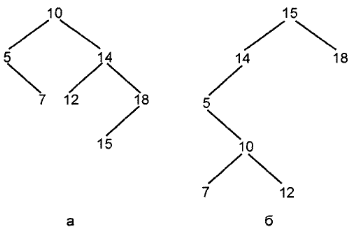
\includegraphics{5,1.png}
	\caption{\textit{Два дерева двоичного поиска}}
\end{figure}

\rindex{Дерево двоичного поиска!представления множеств}
Напишем простую рекурсивную функцию MEMBER(x, А), реализующую тест на принадлежность элемента множеству. Предположим, что элементы множества имеют пока не определенный тип данных, который назовем elementtype. Будем считать, что для этого типа данных определены отношения ''<'' и ''=''. Если это не так, то необходимо написать функции LT(\textit{a, b}) и EQ(\textit{a, b}) такие, что для любых элементов а и b типа elementtype функция LT(\textit{a, b}) будет принимать значение true тогда и только тогда, когда \textit{a} "меньше" \textit{b}, а функция EQ(\textit{a, b}) — когда \textit{a} "равно или больше" \textit{b}.

Тип данных nodetype узлов дерева, содержащих поле element для элементов множества и два поля \textit{leftchild} и \textit{rightchild} указателей на левого и правого сыновей, определим с помощью следующего объявления:
\begin{lstlisting}[language=C, numbers=none]
    typedef struct {
        |\textbf{elementtype}| element;
        |\textbf{nodetype}| leftchild, rightchild;
    } nodetype;
\end{lstlisting}

Далее определим тип SET (Множество) как указатель на узел, который будет корнем дерева двоичного поиска при представлении множества:

\begin{lstlisting}[language=C, numbers=none]
    typedef nodetype SET;
\end{lstlisting}

Теперь можно написать полный код функции MEMBER (листинг 5.1). Отметим, что, поскольку в данном случае SET\rindex{SET!представление посредством дерева двоичного поиска} и указатель на узел — синонимы, функция может вызывать сама себя для проведения поиска по поддереву, как если бы это поддерево представляло все множество. Другими словами, множество можно как бы разбить на подмножество элементов, которые меньше х, и подмножество элементов, больших х.
\begin{lstlisting}[language=C, numbers=none, keepspaces=true, caption={{Процедура MEMBER для дерева двоичного поиска}}]
    bool MEMBER ( const |\textbf{elementtype}| *x, const |\textbf{SET}| *A) {
        /* возвращает true, если элемент х принадлежит множеству А,
        false —  в  противном случае */
        if ( A == NULL)
            return false; /* x не может принадлежать 0 */
        else if ( x == A->element)
            return true;
        else if ( x < A->element)
            return MEMBER(x, A->leftchild);
        else /* x > A->element */
            return MEMBER (x, A->rightchild);
    }; /* MEMBER */
\end{lstlisting}

Процедура INSERT(\textit{x, А}), которая добавляет элемент х в множество А, также проста для написания. Первым действием этой процедуры должна быть проверка условия А = \textbf{nil}, т.е. не является ли множество А пустым. Если это так, то создается новый узел, содержащий х, и А делается указателем на этот узел. Если множество А не
пустое, то, сначала производится поиск элемента, совпадающего с х (это делается примерно так же, как в функции MEMBER). Если элемент х уже есть в множестве,
то никакие действия дальше не производятся. Если же в процессе поиска будет достигнут указатель \textbf{nil} (т.е. дошли до листа дерева), то он заменяется на указатель,
указывающий на новый узел, содержащий элемент х. Код этой процедуры приведен в листинге 5.2.

\begin{lstlisting}[language=C, numbers=none, keepspaces=true,caption={{Вставка нового элемента в дерево двоичного поиска}}]
    void INSERT ( const |\textbf{elementtype}| *x, |\textbf{SET}| *A) {
        if ( A = NULL) {
            new_set(&A);
            A->element    = x;
            A->leftchild  = NULL;
            A->rightchild = NULL;
        }
        else if ( x < A->element)
            INSERT(x-> At->leftchild);
        else if ( x > A->element)
            INSERT(x, At->rightchild);
        /* если х == At->element, то никаких действий
        не производится, т.к -> х уже есть в множестве А */
    }; /* INSERT */
\end{lstlisting}

Удаление элемента представляет некоторые трудности. Сначала надо найти этот элемент в дереве. Если х является листом, то он просто удаляется. Но если х является внутренним узлом (назовем его для краткости \textit{inode}. от interior node — внутренний узел), то его нельзя просто удалить, так как нарушится связанность дерева.

Если \textit{inode} имеет только одного сына (как узел 14 на рис. 5.1,6), то его можно заменить этим сыном. Если \textit{inode} имеет двух сыновей, как узел 10 на рис. 5.1.а, то среди потомков правого сына надо найти элемент с наименьшим значением\footnote[1]{Можно также искать элемент с наибольшим значением среди потомков левого сына.} и заменить им удаляемый элемент. Например, для узла 10 на рис. 5.1.а таким будет узел 12.

Для написания процедуры DELETE полезно иметь функцию DELETEMIN(A), которая удаляет наименьший элемент из непустого дерева и возвращает значение удаляемого элемента. Код функции DELETEMIN приведен в листинге 5.3, а код процедуры DELETE, использующий эту функцию, — в листинге 5.4.

\begin{lstlisting}[language=C, numbers=none, keepspaces=true,caption={{Удаление наименьшего элемента}}]
    |\textbf{elementtype}| DELETEMIN ( |\textbf{SET}| *A ) {
        if ( A->leftchild == NULL) {
        /* А указывает на наименьший элемент */
            DELETEMIN = A->element;
            A = A->rightchild;
        /* замена узла, указанного А, его правым сыном */
        }
        else /* узел, указанный А, имеет левого сына */
            DELETEMIN = DELETEMIN(A->leftchild);
    }; /* DELETEMIN */
\end{lstlisting}

\begin{lstlisting}[language=C, numbers=none, keepspaces=true,caption={{Удаление элемента из дерева двоичного поиска}}]
    void DELETE ( const |\textbf{elementtype}| *x, |\textbf{SET}| *A ) {
        if ( A != NULL)
            if ( x < A->element)
                DELETE(x, A->leftchild);
            else if ( x > A->element)
                DELETE(x, A->rightchild);
            else if ( (A->leftchild== NULL) &&
                            (A->rightchild== NULL))
                A = NULL; /* удаление листа, содержащего х */
            else if ( A->leftchild == NULL)
                A = A->rightchild;
            else if ( A->rightchild == NULL)
                A = A->leftchild;
            else /* у узла есть оба сына */
                A->element = DELETEMIN(A->right->child);
    }; /* DELETE */

\end{lstlisting}

Пример 5.1. Предположим, надо удалить элемент 10 из дерева, показанного на
рис. 5.1.а. В данном случае первым исполняемым оператором в процедуре DELETE будет вызов функции DELETEMIN с аргументом-указателем на узел 14. Этот указатель —
значение поля \textit{rightchild} корня. Результатом этого вызова будет еще один вызов той же функции DELETEMIN. В этом случае ее аргументом будет указатель на узел 12, который находится в поле \textit{leftchild} узла 14. Узел 12 не имеет левого сына, поэтому функция возвращает элемент 12 и устанавливает указатель узла 14 на левого сына в состояние \textbf{nil}. Затем процедура DELETE берет значение 12, возвращенное функцией DELETEMIN, и заменяет им элемент 10. Результирующее дерево показано на рис. 5.2.$\square$

\begin{figure}[ht]
	\center
	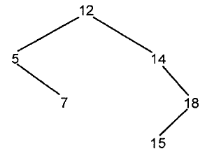
\includegraphics{5,2.png}
	\caption{\textit{Дерево, представленное на
			рис. 5.1.а,  после удаления элемента 10}}
\end{figure}

\section{Анализ времени выполнения операторов} \rindex{Дерево двоичного поиска!время выполнения операторов}
\fancyfoot[LO]{5.2 Анализ времени выполнения операторов}

В этом разделе мы проанализируем работу различных операторов, выполняемых над деревьями двоичного поиска. Мы покажем, что если в первоначально пустое дерево двоичного поиска вставлено \textit{n} произвольных элементов, то средняя длина пути от корня до листа будет \textit{O}(log\textit{n}). Отсюда следует, что среднее время выполнения оператора MEMBER также будет иметь порядок \textit{O}(log\textit{n}).

Легко видеть, что если двоичное дерево полное (т.е. все узлы, за исключением самого нижнего уровня, имеют двух сыновей), то не существует пути, содержащего более 1 + log \textit{n} узлов\footnote[1]{Напомним, что все логарифмы, пока не сказано другое, определены по основанию 2.}. Поэтому операторы MEMBER, INSERT, DELETE и DELETEMIN имеют время выполнения порядка \textit{O}(log\textit{n}). Чтобы доказать это, достаточно заметить, что все эти операторы затрачивают фиксированное время на обработку одного узла, затем рекурсивно вызывают себя для обработки сына рассматриваемого узла. Последовательность узлов, в которых выполняется рекурсивный вызов процедур, формирует путь, исходящий из корня дерева. Поскольку такой путь имеет в среднем длину \textit{O}(log\textit{n}), то и общее время прохождения операторами этого пути будет иметь такой же порядок.

Однако когда элементы вставляются в произвольном порядке, они не обязаны располагаться в виде полного двоичного дерева. Например, если вставка начата с наименьшего элемента и далее элементы вставляются в порядке возрастания, то получим дерево в виде цепочки узлов, где каждый узел имеет правого сына, но не имеет левого. В этом случае, как легко показать, на вставку i-ro элемента требуется O(i) шагов, для завершения всего процесса вставки га элементов необходимо  $\sum_{i=1}^{n}$ i=n(n+1)/2 шагов, т.е. порядка О($n^{2}$), или О(n) на одно выполнение оператора вставки.

Мы должны уметь определять, когда "среднее" дерево двоичного поиска из \textit{n} узлов
ближе по своей структуре к полному двоичному дереву, а когда к цепочке узлов, так
как в первом случае среднее время выполнения операторов имеет порядок \textit{O}(log\textit{n}), а во
втором — \textit{O}(\textit{n}). Если мы не знаем последовательность выполненных (или тех, которые
будут выполнены в будущем) операций вставки и удаления элементов, а также свойства этих элементов (например, мы не можем всегда удалять только минимальные элементы), то естественно предположить, что анализу подлежат только пути "средней"
длины на "случайных" деревьях. В частности, мы вправе предполагать, что деревья
сформированы только вставкой элементов и все последовательности вставляемых элементов равновероятны на фиксированном множестве из n элементов.

\begin{figure}[ht]
	\center
	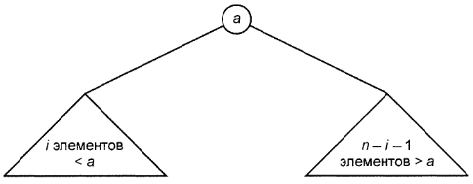
\includegraphics{5,3.png}
	\caption{\textit{Построение дерева двоичного поиска}}
\end{figure}

Принимая эти достаточно естественные предположения, можно вычислить Р(n) —
среднее число узлов в пути от корня до некоторого узла (не обязательно листа). Предполагая, что дерево формируется путем вставки п произвольных элементов в первоначально пустое дерево, очевидно, что Р(0) = 0 и Р(1) — 1. Пусть в списке из n > 2 элементов, готовых к вставке в пустое дерево, первым находится элемент а. Если отсортировать список, то элемент а с равной вероятностью может занимать любое место от 1 до n. Пусть в списке i элементов меньше а, и, следовательно, n — i — 1 элементов больше, чем а. Тогда при построении дерева в его корне поместится элемент а (поскольку он первый элемент списка), i наименьших элементов будут потомками левого сына корня, а оставшиеся n - i - 1 элементов — потомками правого сына корня. Это дерево показано на рис. 5.3.

Так как любые последовательности \textit{i} наименьших элементов и \textit{n - i - 1} наибольших элементов равновероятны, мы вправе предположить, что средняя длина путей в
левом и правом поддеревьях будет \textit{P(i)} и \textit{Р(n - i - 1)} соответственно. Поскольку пути
должны начинаться от корня полного дерева, то к \textit{P(i)} и \textit{Р(n - i - 1)} надо еще прибавить 1. Тогда \textit{Р(n)} можно вычислить путем усреднения для всех \textit{i} от 0 до \textit{n - 1} следующих сумм:

\begin{equation*}
\frac{i}{n}(P(i)+1)+\frac{n-i-1}{n}(P(n-i-1)+1)+\frac{1}{n},
\end{equation*}

где первое слагаемое — средняя длина пути в левом поддереве с весовым коэффициентом i/n, значение второго слагаемого аналогично, а 1/n соответствует "вкладу" в
путь корня. Усредняя эти выражения по всем \textit{i} от 0 до \textit{n} - 1, получим рекуррентное уравнение

\begin{equation}
P(n)=1+\frac{1}{n^2}\sum_{i=0}^{n-1}\left(iP(i)+(n-i-1)P(n-i-1)\right).
\end{equation}

Вторая часть этой суммы $\sum_{i=0}^{n-1}(n-i-1)P(n-i-1)$, если подставить i вместо (n - i - 1), преобразуется в первую часть (5.1) $\sum_{i=0}^{n-1}iP(i)$.В последней сумме слагаемое при i = 0 равно нулю, поэтому суммирование можно начинать с i = 1. Таким образом, формулу (5.1) можно переписать в следующем виде:

\begin{equation}
P(n)=1+\frac{2}{n^2}\sum_{i=n}^{n-1}iP(i), n\geq2
\end{equation}

Теперь индукцией по n покажем, что Р(n) $\leq$ 1 + 41ogn. Очевидно, что это утверждение справедливо для n = 1, поскольку Р(1) = 1, и для n = 2, так как Р(2) = 2 < 1 + 41og2 = 5. Предположим, что оно выполняется для всех i < n. Тогда на основании (5.2) имеем 

\begin{equation}
P(n) \leq 1+\frac{2}{n^2}\sum_{i=1}^{n-1}(4ilogi+i)=1+\frac{2}{n^2}\sum_{i=1}^{n-1}4ilogi +\frac{2}{n^2}\sum_{i=1}^{n-1}i \leq 2+\frac{8}{n^2}\sum_{i=1}^{n-1}ilogi
\end{equation}

Здесь использовано неравенство $\sum_{i=1}^{n-1}i$ $\leq$ $n^2$/2, поэтому $\frac{2}{n^2}\sum_{i=1}^{n-1}i\leq1$. Разделим последнюю сумму в (5.3) на две суммы: по i $\leq$ [n/2],  в этом случае слагаемые не будут превышать ilog(n/2), и по i>[n/2], где слагаемые не превышают ilog(n). Тогда неравенство (5.3) можно переписать так: 
\begin{equation}
P(n) \leq 2+ \frac{8}{n^2}\left( \sum_{i=1}^{[n/2]}ilog(n/2)+\sum_{i=[n/2]+1}^{n-1}ilogn \right).
\end{equation}

Независимо от того, четное или нечетное n, нетрудно показать, что первая сумма в (5.4) не превышает величины $(n^2/8)log(n/2)$, которая равна $(n^2/8)logn-(n^2/8)$,  а вторая не превышает $(3n^2/8)logn$. С учетом этих оценок из (5.4) получаем
\begin{equation*}
P(n) \leq 2+\frac{8}{n^2}\left(\frac{n^2}{2}logn-\frac{n^2}{8}\right) \leq 1+4logn.
\end{equation*}

Этот шаг завершает индукцию и доказывает утверждение. Итак, доказано, что в дереве двоичного поиска, которое получено путем случайной вставки n элементов, средняя длина пути от корня до произвольного узла имеет порядок O(logn), т.е. точно такой же порядок (с точностью до константы пропорциональности), как и для полного двоичного дерева. Более точный анализ показывает, что константу 4 в вышеприведенной оценке можно заменить на 1.4. 

Из доказанного утверждения следует, что время выполнения проверки на принадлежность произвольного элемента к множеству имеет порядок O(logn). Подобный анализ показывает, что если мы включим в путь только те узлы, которые имеют обоих сыновей, или только узлы, имеющие лишь левого сына, то все равно для средней длины пути получим уравнение, подобное (5.1), и поэтому будет оценка порядка O(logn). Отсюда следует вывод, что для выполнения операций проверки на принадлежность к множеству элемента, которого заведомо нет в множестве, вставки произвольного нового элемента или удаления элемента также требуется в среднем времени порядка O(logn).

\subsection*{Эффективность деревьев двоичного поиска} \rindex{Дерево двоичного поиска!эффективность}
\addcontentsline{toc}{subsection}{ Эффективность деревьев двоичного поиска}

При реализации словарей посредством хеш-таблиц время выполнения основных операторов в среднем постоянно, т.е. практически не зависит от размера множеств. Поэтому такая реализация более эффективна, чем реализация деревьев двоичного поиска, за исключением того случая, когда необходимо часто применять оператор MIN, который требует времени порядка О(n) для хеш-таблиц.

Сравним деревья двоичного поиска с частично упорядоченными деревьями\rindex{Частично упорядоченное дерево}, которые применяются для реализации очередей с приоритетами (см. главу 4). Частично упорядоченные деревья из п элементов требуют только O(logn) шагов для выполнения операторов INSERT и DELETEMIN, но не в среднем, а в самом худшем случае. Более того, константа пропорциональности перед logn для частично упорядоченных деревьев меньше, чем для деревьев двоичного поиска. Но на дереве двоичного поиска могут выполняться как операторы DELETE и MIN, так и их комбинация DELETEMIN, тогда как на частично упорядоченном дереве выполняется только последний из этих операторов. Кроме того, оператор MEMBER требует О(n) шагов на частично упорядоченном дереве, но только O(logn) шагов на дереве двоичного поиска. Таким образом, частично упорядоченные деревья хорошо подходят для реализации очередей с приоритетами, но не эффективны при выполнении других операторов множеств, которые могут выполняться на деревьях двоичного поиска.

\section{Нагруженные деревья}
\fancyfoot[LO]{5.3 Нагруженные деревья}

В этом разделе мы рассмотрим специальную структуру для представления множеств, состоящих из символьных строк. Некоторые из описанных здесь методов могут работать и со строками объектов другого типа, например со строками целых чисел. Эта структура называется \textit{нагруженными деревьями}\footnote[1]{ В оригинале структура называется trie, это слово получено из букв, стоящих в середине слова "retrieval" (поиск, выборка, возврат). Устоявшегося термина для этой структуры в русской литературе пока нет. (О расхождении терминологии можно судить по переводу известной книги D£. Knuth. The art of computer programming, Vol. Ill: Sorting and Searching: в первом русском переводе (Кнут Д. Искусство программирования для ЭВМ. Т. 3: Сортировка и поиск. — М., "Мир", 1978 г.) вместо trie используется термин бор (от слова выборка), в последнем переводе переработанного издания этой книги (Кнут Д. Искусство программирования. Т. 3: Сортировка и поиск. — М., Издательский дом "Вильяме", 2000 г.) — термин луч (от слова получение).) Чтобы не заниматься "терминотворчеством", мы применили известный термин нагруженные деревья, который соответствует смыслу этой структуры. В данном случае можно было бы применить и термин синтаксические деревья, но, хотя этот термин по своему значению и "пересекается" с термином нагруженные деревья, он имеет другую направленность. — Прим. ред.}
(tries). Рассмотрим их применение к символьным строкам.

Пример 5.2. Как описывалось в главе 1, возможная реализация проверки орфографии состоит из следующей последовательности действий: сначала читается слово из текстового файла с остановкой после каждого слова (слова отделяются друг от друга пробелом или символом новой строки), далее проверяется, есть ли это слово в стандартном словаре наиболее употребительных слов. Слова, отсутствующие в словаре, распечатываются как возможные ошибки. В листинге 5.5 приведен эскиз возможной программы \textit{spell} (правописание). Здесь использована процедура \textit{getword(x, f)}, которая читает следующее слово в текстовом файле \textit{f} и присваивает его переменной х, имеющей тип wordtype (мы определим его позже). Еще одна используемая переменная А имеет знакомый нам тип SET\rindex{SET}. Реализация этого АТД использует операторы INSERT, DELETE, MAKENULL и PRINT. Последний оператор распечатывает элементы множества. $\square$

\begin{lstlisting}[language=C, numbers=none, keepspaces=true,caption={{Программа проверки орфографии}}]
    typedef /* надо определить */ wordtype
    typedef /* надо определить, используя структуру 
                                        нагруженного дерева */ SET

    |\textbf{SET}| A; /* хранит считанное слово, пока оно не найдено в словаре */
    |\textbf{wordtype}| nextword;
    FILE *dictionary;

    void getword ( const |\textbf{wordtype}| *x, FILE *f);
        /* читает следующее слово в файле f и
                присваивает его переменной х */
    void INSERT ( const wordtype *х, SET *S);
        /* надо определить */
    void DELETE ( const wordtype *x, SET *S);
        /* надо определить */
    void MAKENULL ( SET *S);
        /* надо определить */
    void PRINT ( SET *S );
        /* надо определить */

    void spell(FILE *input, FILE *output, FILE *dictionary) {
        MAKENULL(A);
        while (!feof(input)) {
            getword(nextword, input);
            INSERT (nextword, A)
        }
        while (!feof(dictionary)) {
            getword (nextword, dictionary);
            DELETE  (nextword, A)
        }
        PRINT(A)
    }; /* spell */
\end{lstlisting}

Структура нагруженных деревьев поддерживает операторы множеств, у которых элементы являются словами, т.е. символьными строками. Удобно, когда большинство слов начинается с одной и той же последовательности букв или, другими словами, когда количество различных префиксов значительно меньше общей длины всех слов множества.

В нагруженном дереве каждый путь от корня к листу соответствует одному слову из множества. При таком подходе узлы дерева соответствуют префиксам слов множества. Чтобы избежать коллизий слов, подобных THE и THEN, введем специальный символ \$, \textit{маркер конца}, указывающий окончание любого слова. Тогда только слова будут словами, но не префиксы. 

Пример 5.3. На рис. 5.4 показано нагруженное дерево\rindex{Нагруженное дерево} слов {THE, THEN, THIN, THIS, TIN, SIN, SING}. Здесь корень соответствует пустой строке, а два его сына — префиксам Т и S. Самый левый лист представляет слово THE, следующий лист — слово THEN и т.д.



\begin{figure}[ht]
	\center
	\includegraphics{5,4.png}
	\caption{\textit{Нагруженное дерево}}
\end{figure}

На основании рис. 5.4 можно сделать следующие выводы.

1. Каждый узел может иметь до 27 сыновей\footnote[1]{Здесь предполагается, что алгоритм работает только с английским алфавитом. — Прим. ред.}, которые могут быть буквами или символом \$.

2. Большинство узлов имеет значительно меньше 27 сыновей. 

3. Листом может быть только окончание ребра, помеченного символом \$.

\subsection*{Узлы нагруженного дерева как АТД}
\addcontentsline{toc}{subsection}{ Узлы нагруженного дерева как АТД}
\rindex{Нагруженное дерево!узлы}

Мы можем рассматривать узел нагруженного дерева как отображение, где областью определения будет множество \{А, В, .... Z, \$\} (или другой выбранный алфавит), а множеством значений — множество элементов типа "указатель на узел нагруженного дерева". Более того, так как дерево можно идентифицировать посредством его корня, то АТД TRIE\rindex{Trie} \rindex{Абстрактный тип данных!TRIE} (Нагруженное дерево) и TRIENODE\rindex{TRIENODE} \rindex{Абстрактный тип данных TRIENODE} (Узел нагруженного дерева) имеют один и тот же тип данных, хотя операторы, используемые в рамках этих АТД, имеют существенные различия. Для реализации АТД TRIENODE\rindex{TRIENODE!операторы} необходимы следующие операторы\rindex{Операторы!узлов нагруженного дерева}. 

1. Процедура ASSIGN(\textit{node, с, р}), которая задает значение \textit{р} (указатель на узел) символу \textit{с} в узле \textit{node}, 

2. Функция VALUEOF\rindex{Оператор!VALUEOF}(\textit{node, с})\footnote[2]{Эта функция является версией функции COMPUTER из раздела 2.5.} — возвращает значение (указатель на узел), ассоциированное с символом \textit{с} в узле \textit{node}.

3. Процедура GETNEW\rindex{Оператор!GETNEW}(\textit{node, с}) делает значение узла \textit{node} с символом \textit{с} указателем на новый узел.

Нам также будет необходима процедура MAKENULL(\textit{node}), делающая узел \textit{node} пустым отображением

Самой простой реализацией узлов нагруженного дерева будет массив \textit{node} указателей на узлы с индексным множеством \{А, В, ..., Z, \$\}. Таким образом, АТД TRIENODE\rindex{TRIENODE!определение} можно определить следующим образом: 

\begin{lstlisting}[language=C, numbers=none]
    typedef enum {
        'A', 'B', ... 'Z', '\$'
    }
    chars;
    TRIENODE == array[chars] of T TRIENODE;
\end{lstlisting}


Если \textit{node} — массив узлов, то \textit{node}[c] совпадает с VALUEOF(\textit{node, с}) для любого символа \textit{с}. Чтобы избежать создания многочисленных листьев, являющихся потомками '\$', примем соглашение, что \textit{node}['\$'] имеет значение \textbf{nil} или указателя на самого себя. (При формировании дерева \textit{node} не может иметь сына, соответствующего '\$', но после возможных преобразований может появиться такой сын, которого мы никогда не создавали.) Теперь можно написать процедуры, выполняемые над узлами нагруженного дерева. Их код приведен в следующем листинге.
\newpage

\begin{lstlisting}[language=C, numbers=none, keepspaces=true,caption={{ Операторы узлов нагруженного дерева }}]
    void MAKENULL (|\textbf{TRIENODE}| node) {
        /* делает node листом, т.е. пустым отображением */
        chars с;
        for (c = 'A'; c <= '\$'; c = next_c(c))
            node[с] = NULL;
    } /* MAKENULL */

    void ASSIGN (|\textbf{TRIENODE}| node, char c, |\textbf{TRIENODE}| p) {
        node[c] = p;
    } /* ASSIGN */

    |\textbf{TRIENODE}| VALUEOF (|\textbf{TRIENODE}| node, char c) {
        return(node[c]);
    } /* VALUEOF */

    void GETNEW ( |\textbf{TRIENODE}| node, char c ) {
        new(node[c]);
        MAKENULL(node[c])
    } /* GETNEW */
\end{lstlisting}

Теперь определим АТД TRIE: 
\begin{lstlisting}[language=C, numbers=none]
    typedef TRIENODE TRIE;
\end{lstlisting}

Мы можем определить тип wordtype как массив символов фиксированной длины. Предполагается, что среди значений такого массива обязательно есть по крайней мере один символ '\$'. Считаем, что концу слова соответствует первый символ '\$', независимо от того, что за ним следует. При выполнении этих предположений написана процедура INSERT(\textit{x, words}), которая вставляет слово \textit{х} в множество \textit{words} (слова), представленное посредством нагруженного дерева. Код этой процедуры показан в листинге 5.7. Написание процедур MAKENULL, DELETE и PRINT для данной реализации нагруженных деревьев оставляем в качестве упражнений для читателей.

\begin{lstlisting}[language=C, numbers=none, keepspaces=true,caption={{Процедура INSERT}}]
    void INSERT ( const |\textbf{wordtype}| *х, |\textbf{TRIE}| *words) {
        int   i; /* считает позиции в слове х */
        |\textbf{TRIE}| *t; /* используется для указания на узлы дерева, 
                                соответствующие префиксу слова х */

        i = 1;
        t = words;

        while (x[i] != '\$') {
            if ( VALUEOF(t), x[i]) == NULL)
            /* если текущий узел не имеет сына для символа x[i],
                    то он создается */
                GETNEW(t, x[i]);
            t = VALUEOF(t), x[i]);
            /* продвижение к сыну узла t для символа х[1] */
            i = i + 1; /* перемещение далее по слову х */
        }
        /* в слове х достигнут первый символ '\$' */
        ASSIGN(t, '\$', t);
    /* делает петлю на '\$' для создания листа */
    } /* INSERT */
\end{lstlisting}
\newpage

\subsection*{Представление узлов нагруженного дерева посредством списков} \rindex{Нагруженное дерево!представление узлов посредством списков}
\addcontentsline{toc}{subsection}{ Представление узлов нагруженного дерева посредством списков}

Множество слов, которые имеют р различных префиксов и для хранения требуют 27р байт, можно представить посредством реализации узлов нагруженного дерева с помощью массивов фиксированной длины. Величина 27р байт может значительно превышать общую длину слов в множестве. Существует другая реализация нагруженных деревьев, которая экономит используемый объем памяти. Напомним, что мы рассматриваем каждый узел нагруженного дерева как отображение (см. раздел 2.6). В принципе, можно применить любую реализацию отображений, но мы хотим найти наиболее подходящую, область определения которых сравнительно мала. При таком условии наилучшим выбором будет реализация отображения посредством связанных списков. Здесь представлением отображения, т.е. узла нагруженного дерева, будет связанный список символов, для которых соответствующие значения не являются указателями \textbf{nil}. Такое представление можно сделать с помощью следующего объявления: 

\begin{lstlisting}[language=C, keepspaces=true,numbers=none]
    typedef struct{
        chars domain;
        |\textbf{Tcelltype}| value;
        /*указатель на первую ячейку списка узла сына*/
        |\textbf{Tcelltype}| next;
        /*указатель на следующую ячейку списка*/
    }
\end{lstlisting}


Мы оставляем в качестве упражнений написание для данной реализации процедур ASSIGN, VALUEOF, MAKENULL и GETNEW. После создания этих процедур процедура INSERT из листинга 5.7 должна стать работоспособной программой.

\subsection*{Эффективность структуры данных нагруженных деревьев}
\addcontentsline{toc}{subsection}{ Эффективность структуры данных нагруженных деревьев}
\rindex{Нагруженное дерево!эффективность}

Для хеш-таблиц и нагруженных деревьев сравним необходимое время выполнения операторов и занимаемый объем памяти для представления \textit{n} слов с \textit{р} различными префиксами и общей диной слов \textit{l}. Будем предполагать, что указатели требуют для своего хранения по 4 байт на указатель. По всей видимости, наиболее эффективными по критерию требуемой памяти и поддержке операторов INSERT и DELETE будут хеш-таблицы. Если слова имеют разную длину, то ячейки сегментов хештаблицы не будут непосредственно содержать слова, а только два указателя. Один требуется для связи ячеек сегмента, а другой будет указывать на начало слова, соответствующего сегменту. 

Сами слова хранятся в большом символьном массиве, где начало и конец каждого слова помечается специальным маркером, таким как '\$'. Например, слова THE, THEN и THIN будут храниться как 

\begin{equation*}
\text{THE\$THEN\$THIN\$ \dots}
\end{equation*}

Указателями для этих слов будут курсоры, указывающие на позиции 1, 5 и 10 массива. Подсчитаем пространство, занимаемое сегментами хеш-таблицы и массивом символов. 

1. 8\textit{n} байт для ячеек сегментов — по одной ячейке на слово. Ячейка содержит два указателя, т.е. занимает 8 байт, которые умножаются на \textit{n} (количество слов). 

2. \textit{l} + \textit{n} байт для символьного массива, хранящего \textit{n} слов общей длиной \textit{l} и \textit{n} разделителей слов. 

Таким образом, общее занимаемое пространство составляет 9\textit{n} + \textit{l} плюс пространство, используемое для заголовков сегментов.

Для сравнения: нагруженное дерево с узлами, представленными связанными списками, требует \textit{р} + \textit{n} ячеек — по одной ячейке на каждый префикс и по одной ячейке на каждое окончание слова. Каждая ячейка содержит символ и два указателя, т.е. всего 9 байт. Поэтому общее занимаемое пространство составляет 9\textit{р} + 9\textit{n} байт. Если \textit{l} и пространство заголовков сегментов больше 9\textit{р}, то нагруженное дерево 

\noindent занимает меньше пространства, чем хеш-таблица. Но в реальных приложениях, таких как словари, отношение \textit{l/p} обычно меньше 3, поэтому в этих приложениях хеш-таблицы более экономичны. 

С другой стороны, к достоинствам нагруженных деревьев можно отнести возможность перемещения по дереву и выполнения таких операторов, как INSERT, DELETE и MEMBER, за время, пропорциональное длине "обслуживаемого" слова. Хеш-функция, чтобы быть действительно "случайной", хеширует каждый символ слова. Поэтому ясно, что вычисления хеш-функции требуют примерно такого же времени, как и выполнение, например, оператора MEMBER для нагруженного дерева. И, конечно, время вычисления хеш-функции не включает время, необходимое для разрешения коллизий или выполнения операций вставки, удаления или поиска. Поэтому мы вправе ожидать, что нагруженные деревья будут работать значительно быстрее со словарями, состоящими из символьных строк, чем хеш-таблицы. 

Другим достоинством нагруженных деревьев является то, что, в отличие от хештаблиц, они поддерживают эффективное выполнение оператора MIN. Кроме того, если хеш-таблица построена так, как описано выше, то после удаления слова из словаря здесь нельзя сравнительно просто организовать повторное использование освободившегося пространства в массиве символов.
\rindex{Дерево двоичного поиска|)}
\section{Реализация множеств посредством сбалансированных деревьев}\rindex{Множество!представление посредством сбалансированного дерева}\rindex{Дерево!сбалансированное}

\fancyfoot[LO]{5.4 Реализация множеств посредством сбалансированных деревьев}

В разделах 5.1 и 5.2 мы рассмотрели способы представления множеств посредством
деревьев двоичного поиска и узнали, что операторы\rindex{Операторы!2-3 дерева}, подобные INSERT, выполняются
за время, пропорциональное средней длине пути в этом дереве. Затем мы показали, что
средняя глубина узлов составляет \textit{O}(log\textit{n}) для "случайного" дерева из \textit{n} узлов. Однако
некоторые последовательности операций вставки и удаления узлов дерева могут привести к деревьям двоичного поиска, чья средняя глубина будет пропорциональна n. Это
наводит на мысль попытаться после каждой вставки или удаления реорганизовать дерево так, чтобы оно всегда было полно, тогда время выполнения оператора INSERT и
других подобных операторов всегда будет иметь порядок \textit{O}(log\textit{n}).

На рис. 5.5,а показано дерево из шести узлов, а на рис. 5.5,6 — то же дерево (уже
полное) после вставки седьмого узла с элементом 1. Но обратите внимание, что каждый узел на рис. 5.5,6 имеет другого родителя, отличного от родителя, изображенного на рис. 5.5,а. Отсюда следует, что надо сделать \textit{n} шагов при вставке элемента 1,
чтобы сохранить дерево по возможности сбалансированным. Это значительно хуже,
чем в случае простой вставки в полное дерево двоичного поиска при реализации словарей, очередей с приоритетами и других АТД, где оператор INSERT (и другие ему
подобные) требует времени порядка \textit{O}(log\textit{n}).

\begin{figure}[ht]
	\center
	\includegraphics{5,5.png}
	\caption{\textit{Полные деревья}}
\end{figure}

Существуют другие подходы к реализации словарей и очередей с приоритетами,
где даже в самом худшем случае время выполнения операторов имеет порядок
\textit{O}(log\textit{n}). Мы подробно рассмотрим одну из таких реализаций, которая называется 2-3
дерево\rindex{Множество!реализация посредством 2-3 дерева} \rindex{Дерево 2-3(2-3 дерево)}и имеет следующие свойства.


1. Каждый внутренний узел имеет или два, или три сына.

2. Все пути от корня до любого листа имеют одинаковую длину.

Будем считать, что пустое дерево и дерево с одним узлом также являются 2-3 деревьями.

Рассмотрим представления множеств, элементы которых упорядочены \\посредством некоторого отношения линейного порядка, обозначаемого символом ''<''. 
Элементы множества располагаются в листьях дерева, при этом, если элемент \textit{а} располагается левее элемента \textit{b}, справедливо отношение \textit{а} < \textit{b}. Предполагаем, что упорядочивание элементов по используемому отношению линейного порядка основывается
только на значениях одного поля (среди других полей записи, содержащей информацию об элементе), которое формирует тип элементов. Это поле назовем ключом. Например, если элементы множества — работники некоторого предприятия, то ключевым полем может быть поле, содержащее табельный номер или номер карточки социального страхования.

В каждый внутренний узел записываются ключ наименьшего элемента, являющегося потомком второго сына, и ключ наименьшего элемента — потомка третьего сына, если, конечно, есть третий сын\footnote[1]{Существуют другие разновидности 2-3 деревьев, когда во внутренний узел помещаются
	целые записи, как это делается в деревьях двоичного поиска.}. На рис. 5.6 показан пример 2-3
дерева. В этом и последующих примерах мы идентифицируем элементы с их ключевым полем, так что порядок элементов становится очевидным.

\begin{figure}[ht]
	\center
	\includegraphics{5,6.png}
	\caption{\textit{2-3 дерево}}
\end{figure}

Отметим, что 2-3 дерево с $k$ уровнями имеет от $2^{k - 1}$ до $3^{k - 1}$ листьев. Другими
словами, 2-3 дерево, представляющее множество из \textit{n} элементов, будет иметь не
менее 1 + $log_3$\textit{n} и не более 1 + $log_2$\textit{n} уровней. Таким образом, длины всех путей будут иметь порядок \textit{O}(log\textit{n}).

Можно найти запись с ключом \textit{x} в множестве, представленном 2-3 деревом, за
время \textit{O}(log\textit{n}) путем простого перемещения по дереву, руководствуясь при этом значениями элементов, записанных во внутренних узлах. Во внутреннем узле \textit{node} ключ \textit{х} сравнивается со значением у наименьшего элемента, являющегося потомком второго сына узла \textit{node}. (Напомним, что мы трактуем элементы так, как будто они состоят только из одного ключевого поля.) Если \textit{х} < \textit{у}, то перемещаемся к первому сыну узла
\textit{node}. Если \textit{х} $\geq$ \textit{у} и узел \textit{node} имеет только двух сыновей, то переходим ко второму
сыну узла \textit{node}. Если узел \textit{node} имеет трех сыновей и \textit{х} $\geq$ \textit{у}, то сравниваем \textit{х} со значением \textit{z} — вторым значением, записанным в узле \textit{node}, т.е. со значением наименьшего элемента, являющегося потомком третьего сына узла \textit{node}. Если \textit{х} < \textit{z}, то переходим ко второму сыну, если \textit{х} $\geq$ \textit{z}, переходим к третьему сыну узла \textit{node}. Таким
способом в конце концов мы придем к листу, и элемент \textit{х} будет принадлежать исходному множеству тогда и только тогда, когда он совпадает с элементом, записанным в листе. Очевидно, что если в процессе поиска получим \textit{х} = \textit{у} или \textit{х} = \textit{z}, поиск
можно остановить. Но, конечно, алгоритм поиска должен предусмотреть спуск до
самого листа.


\subsection*{Вставка элемента в 2-3 дерево} \rindex{Дерево 2-3(2-3 дерево)!вставка элемента}
\addcontentsline{toc}{subsection}{ Вставка элемента в 2-3 дерево}

Процесс вставки нового элемента х в 2-3 дерево начинается так же, как и процесс
поиска элемента \textit{х}. Пусть мы уже находимся на уровне, предшествующем листьям, в
узле \textit{node}, чьи сыновья (уже проверено) не содержат элемента \textit{х}. Если узел \textit{node} имеет двух сыновей, то мы просто делаем элемент \textit{х} третьим сыном, помещая его в правильном порядке среди других сыновей. Осталось переписать два числа в узле \textit{node} в
соответствии с новой ситуацией.

Например, если мы вставляем элемент 18 в дерево, показанное на рис. 5.6, то узлом \textit{node} здесь будет самый правый узел среднего уровня. Помещаем элемент 18 среди сыновей этого узла, упорядочивая их как 16, 18 и 19. В узле \textit{node} записываются
числа 18 и 19, соответствующие второму и третьему сыновьям. Результат вставки
показан на рис. 5.7.

\begin{figure}[ht]
	\center
	\includegraphics{5,7.png}
	\caption{\textit{2-3 дерево с вставленным элементом 18}}
\end{figure}

Предположим, что элемент \textit{x} будет четвертым, а не третьим сыном узла \textit{node}.
В 2-3 дереве узел не может иметь четырех сыновей, поэтому узел \textit{node} разбивается на два узла, которые назовем \textit{node} и \textit{node'}. Два наименьших элемента из четырех станут сыновьями нового узла \textit{node}, а два наибольших элемента — сыновьями узла \textit{node'}. Теперь надо вставить узел \textit{node'} среди сыновей узла \textit{р} — родителя узла \textit{node}. Здесь ситуация аналогична вставке листа к узлу \textit{node}. Так, если узел \textit{р} имеет двух сыновей, то узел \textit{node'} становится третьим (по счету) сыном этого узла и помещается непосредственно справа от узла \textit{node}. Если узел \textit{р} уже имеет трех сыновей, то он разбивается на два узла \textit{р} и \textit{р'}, узлу \textit{р} приписываются два наименьших сына, а узлу \textit{р'} — оставшиеся. Затем рекурсивно вставляем узел \textit{р'} среди сыновей родителя узла \textit{р} и т.д.

\begin{figure}[ht]
	\center
	\includegraphics[scale = 0.9]{5,8.png}
	\caption{\textit{Вставка элемента 10 в 2-3 дерево из рис. 5.7}}
\end{figure}
\newpage

Особый случай возникает при необходимости разбиения корня дерева. В этой ситуации создается новый корень, чьими сыновьями будут два узла, полученные в результате разбиения старого корня. Очевидно, в этом случае количество уровней 2-3 дерева возрастает на единицу.

\textbf{Пример 5.4.} Предположим, что надо вставить элемент 10 в дерево, показанное на рис. 5.7. Намеченный родитель для нового элемента уже имеет трех сыновей 7, 8 и 12, поэтому он разбивается на два узла. Первый узел будет иметь сыновей 7 и 8, а второй — 10 и 12. Результат этого разбиения показан на рис. 5.8,а. Теперь необходимо вставить новый узел (с сыновьями 10 и 12) среди сыновей корня дерева. С этим узлом корень будет иметь четыре сына, поэтому он разбивается на два узла и образуется новый корень, как показано на рис. 5.8,6. Подробности реорганизации информации об элементах будут показаны далее при разработке программы для оператора INSERT.$\square$

\subsection*{Удаление элемента из 2-3 дерева} \rindex{Дерево 2-3(2-3 дерево)!удаление элемента}
\addcontentsline{toc}{subsection}{ Удаление элемента из 2-3 дерева}

При удалении листа может случиться так, что родитель \textit{node} этого листа останется только с одним сыном. Если узел \textit{node} является корнем, то единственный сын становится новым корнем дерева. Для случая, когда узел \textit{node} не является корнем, обозначим его родителя как \textit{р}. Если этот родитель имеет другого сына, расположённого слева или справа от узла \textit{node}, и этот сын имеет трех сыновей, то один из них становится сыном узла \textit{node}. Таким образом, узел \textit{node} будет иметь двух сыновей. Если сын родителя \textit{р}, смежный с узлом \textit{node}, имеет только двух сыновей, то единственный сын узла \textit{node} присоединяется к этим сыновьям, а узел \textit{node} удаляется. Если после этого родитель \textit{р} будет иметь только одного сына, то повторяется описанный процесс с заменой узла \textit{node} на узел \textit{р}.

\textbf{Пример 5.5.} Удалим элемент 10 из дерева, представленного на рис. 5.8,6. После удаления этого элемента его родитель будет иметь только одного сына. Но его "дедушка" имеет другого сына, у которого, в свою очередь, есть три сына: элементы 16, 18 и 19. Этот узел находится справа от неполного узла, поэтому лист с наименьшим элементом 16 переносится в неполный узел. В результате получим дерево, показанное на рис. 5.9,а.

Пусть далее надо удалить из полученного дерева элемент 7. После удаления его родитель будет иметь только одного сына 8, а его "дедушка" не имеет сыновей с тремя "детьми". Поэтому делаем элемент 8 "братом" элементов 2 и 5, как показано на рис. 5.9,6. На этом рисунке узел, помеченный звездочкой, имеет только одного сына, а его родитель не имеет сыновей с тремя "детьми". Поэтому мы удаляем помеченный узел, присоединяя его сына к узлу, расположенному справа от помеченного узла. Теперь корень будет иметь только одного сына, поэтому он также удаляется. В результате получим дерево, показанное на рис. 5.9,в.

\begin{figure}[ht]
	\center
	\includegraphics[scale = 0.9]{5,9.png}
	\caption{\textit{Удаление элемента 7 из 2-3 дерева}}
\end{figure}

Из вышеприведенных примеров видно, что часто приходится манипулировать значениями внутренних узлов. Мы всегда сможем вычислить эти значения, если будем помнить наименьшие значения всех потомков узлов, составляющих путь от дерева до удаляемого листа. Эту информацию можно получить путем рекурсивного применения алгоритма удаления, вызываемого для каждого узла, составляющего путь, который начинается от корня дерева. Возникающие при этом ситуации учтены при написании программы (см. далее), реализующей оператор DELETE. $\square$

\subsection*{Типы данных для 2-3 деревьев} \rindex{Дерево 2-3(2-3 дерево)!тип данных узлов}
\addcontentsline{toc}{subsection}{ Типы данных для 2-3 деревьев}

Ограничимся представлением (посредством 2-3 деревьев) множеств элементов, чьи ключи являются действительными числами. Природа других полей, которые вместе с полем \textit{key} (ключ) составляют запись об элементе, пока не определена и здесь нас не интересует; общий тип записи обозначим как elementtype.

При написании программ на языке Pascal родители листьев должны быть записями, содержащими два поля действительных чисел (ключи наименьших элементов во втором и в третьем поддеревьях) и три поля указателей на элементы. Родители этих узлов являются записями, состоящими из двух полей действительных чисел и трех полей указателей на родителей листьев. Таким образом, разные уровни 2-3 дерева имеют разные типы данных (указатели на элементы или указатели на узлы). Эта ситуация вызывает затруднения при программировании на языке Pascal операторов, выполняемых над 2-3 деревьями. К счастью, язык Pascal имеет механизм, вариант структуры \textbf{record} (запись), который позволяет обращаться с узлами 2-3 дерева, имеющими разный тип данных\footnote[1]{В данном случае все равно каждый узел будет занимать пространство, равное пространству, занимаемому самым "большим" типом данных. Поэтому язык Pascal — не лучший язык для практической реализации 2-3 деревьев.}. В листинге 5.8 приведено объявление типов данных для узлов 2-3 дерева, а также для типа данных SET\rindex{SET} (Множество), представляющего 2-3 дерево, в виде указателя на корень этого дерева.

\begin{lstlisting}[language=C, numbers=none, keepspaces=true,caption={{Объявление типов данных узлов 2-3 дерева}}]
    typedef struct {
        double key;
        /* объявление других полей, если необходимо */
    } elementtype;

    typedef enum {
        leaf, interior;
    } nodetype;
    /* объявление типа узла, содержащее поля leaf (лист) и
            interior (внутренний узел) */
    typedef struct {
        union {
            struct {
                |\textbf{elementtype}| element;
            } s_leaf;

            struct {
                thowthreenode *firstchild,
                *secondchild, *thirdchild;
                double lowofsecond, lowofthird;
            } s_interior;
        } val;
    } thowthreenode;

    typedef SET *twothreenode;
\end{lstlisting}


\subsection*{Реализация оператора INSERT}
\addcontentsline{toc}{subsection}{ Реализация оператора INSERT}

Детали реализации операторов для 2-3 деревьев \rindex{Дерево 2-3(2-3 дерево)!операторы}несколько запутанны, но принципы просты. Поэтому подробно мы опишем только оператор вставки. Реализации операторов удаления, проверки на принадлежность множеству и других подобны реализации оператора INSERT, а оператор нахождения минимального элемента выполняется просто спуском по самому левому пути дерева. Оператор INSERT реализован как основная программа, вызывающая корень дерева и процедуру \textit{insertl}, которая рекурсивно вызывается для узлов дерева. Для определенности мы предполагаем, что 2-3 дерево не является пустым деревом и содержит более одного узла. Последние два случая, когда дерево пустое или содержит только один узел, реализуются простой последовательностью шагов, которые читатель может написать самостоятельно.

Функция \textit{insertl} должна возвращать как указатель на новый узел, если он будет создан, так и ключ наименьшего элемента, находящегося ниже нового узла. В языке Pascal механизм создания такой функции достаточно сложен, поэтому мы объявили \textit{insertl} как процедуру, которая присваивает значения параметрам \textit{pnew} и \textit{low} при создании нового узла. В листинге 5.9 показан эскиз этой процедуры, а ее полный код приведен в листинге 5.10.

\begin{lstlisting}[language=C, numbers=none, keepspaces=true,caption={{Процедура вставки в 2-3 дерево}}]
    void insertl (
    const |\textbf{twothreenode}| *node,
    const val.s_leaf.elementtype *x,	
    /* элемент х должен быть вставлен в поддерево с корнем node */
    |\textbf{twothreenode}| pnew,      /* указатель на новый элемент */
    double *low 
    /* наименьший элемент в поддереве с корнем,
    на который указывает pnew */) {
        pnew = NULL;
        if ( node является листом) {
            if ( x не является элементом, содержащимся в node) {
                создание нового узла, указанного pnew;
                сделать х элементом, содержащимся в новом узле;
                *low = x->key;
            }
        }
        else { /* node является внутренним узлом */
            выбрать w — сына узла node;
        insertl(w, x, pback, lowback);
        if ( pback != NULL) {
            вставка указателя pback среди детей узла node,
            расположенных справа от w;
            if ( node имеет четырех сыновей) {
                создание нового узла, указанного pnew;
                создание нового узла для третьего и
                четвертого сыновей node;
                задание значений полям
                val.s_interior.lowofsecond
                и val.s_interior.lowofthird
                для узла node и нового узла;
                задание полю *low наименьшего ключа
                среди детей нового узла;
            }
        }
    } /* insertl */
\end{lstlisting}
\newpage
\begin{lstlisting}[language=C, numbers=none, keepspaces=true,caption={{Полный код процедуры \textit{insertl}}}]
    void insert1 ( const twothreenode *node, elemnttype *x,
            twothreenode pnew, double *low ) {
        |\textbf{twothreenode}| *pback;
        double lowback;
        ... child; /* указывает на следующего "обрабатываемого" 
                        сына node ( ср. с w в листинге 5->9) */
        |\textbf{twothreenode}| w; /* указатель на сына */
        pnew = NULL;
        if ( node->kind == leaf ) {
            if ( node->val.s_leaf.element->key != x->key ) {
                /* создание нового листа, содержащего х и
                        "возврат" этого листа */
                new(pnew, leaf);
                if ( node->val.s_leaf.element->key < x->key ) {
                    /* запись х в новый узел */
                    pnew->val.s_leaf.element = x;
                    *low = x->key;
                }
                else {
                    pnew->val.s_leaf.element =
                    node->val.s_leaf.element;
                    node->val.s_leaf.element  = x;
                    *low = pnewl->val.s_leaf.element->key
                }
            }
        }
        else { /* node является внутренним узлом */
                /* выбор следующего сына node */
            if ( x->key < node->val.s_interior.lowofsecond ) {
                child = 1;
                w = node->val.s_interior.firstchild;
            }
            else if ((node->val.s_interior.thirdchild == NULL) ||
                (x->key < node->val.s_interior.lowofsecond)) {
                child = 2; /* х во втором поддереве */
                w = node->val.s_interior.secondchild;
            }
            else { /* х в третьем поддереве */
                child = 3;
                w  = node->val.s_interior.thirdchild
            }
        insert(w, x, pback, lowback);
        if ( pback != NULL) /* надо вставить нового сына node */
            if ( node->val.s_interior.thirdchild == NULL) {
                /* node имеет только двух сыновей */
                if ( child - 2) {
                    node->val.s_interior.thirdchild =
                    pback;
                    node->val.s_interior.lowofthird = 
                    lowback;
                }
                else { /* child == 1 */
                    node->val.s_interior.thirdchild =
                    node->val.s_interior.secondchild;
                    node->val.s_interior.lowofthird = 
                    node->val.s_interior.lowofsecond;
                    node->val.s_interior.secondchild =
                    pback;
                    node->lonrofsecond = lowback;
                }
                else { /* node уже имеет трех сыновей */
                    new(pnew, interior);
                    if ( child == 3 ) {
                    /*pback и третий сын становятся
                        сыновьями нового узла*/
                        pnew->val.s_interior.firstchild =
                        node->val.s_interior.thirdchild;
                        pnew->val.s_interior.secondchild =
                        pback;
                        pnewl->val.s_interior.thirdchild =
                        NULL;
                        pnet->val.s_interior.lowofsecond =
                        lowback;
                    /* *lowDfthird для pnew неопределен */			
                        *low = node->val.s_interior.lowofthird;
                        node->val.s_interior.thirdchild = NULL;
                    }
                    else {/*child < 2; перемещение третьего
                                        сына node к pnew*/
                        pnew->val.s_interior.secondchild =
                        node->val.s_interior.thirdchild;
                        pnew->val.s_interior.lowofsecond =
                        node->val.s_interior.lowofthird;
                        pnew->val.s_interior.thirdchild =
                        NULL;
                        node->thirdchild  = NULL;
                    }
                if ( child == 2 ) {
                    /* pback становится первым
                    сыном pnew */
                    pnewf->val.s_interior.firstchild =
                    pback;
                    *low = lowback;
                }
                if ( child == 1 ) {
                    /* 2-й сын node перемещается к pnew,
                    pback становится 2-м сыном node */
                    pnew->val.s_interior.firstchild =
                    node->val.s_interior.secondchild;
                    *low =
                    node - val.s_interior.lowofsecond;
                    node->val.s_interior.secondchild =
                    pback;
                    node->val.s_interior.lowofsecond =
                    lowback;
                }
            }
        }
    }
} /* insert1 */
\end{lstlisting}
\newpage

Теперь можно написать процедуру INSERT, которая вызывает \textit{insertl}. Если \textit{insertl} "возвращает" новый узел, тогда INSERT должна создать новый корень дерева. Код процедуры INSERT представлен в листинге 5.11. Здесь мы считаем, что тип SET — это тип Ttwothreenode, т.е. указатель на корень 2-3 дерева, чьи листья содержат элементы исходного множества.

\begin{lstlisting}[language=C, numbers=none, keepspaces=true,caption={{Оператор INSERT для множеств, представленных посредством 2-3 деревьев}}]
    void INSERT ( const |\textbf{elementtype}| *x, |\textbf{SET}| *S) {
        |\textbf{twothreenode}| *pback; /*указатель на узел, 
                                    возвращенный insertl*/
        double lowback; /*наименьшее (low) значение 
                        в поддереве pback*/
        |\textbf{SET}| saves; /* для временного хранения копии указателя S */
            /* здесь надо вставить процедуру проверки, 
            которая выясняет, является ли S пустым деревом 
            или имеет только один узел, и уществляет 
            для этих ситуаций вставку */
        insertl(S, x, pback, lowback);
        if ( pback != NULL ) {
            /* создание нового корня,
                на его сыновей указывают S и pback */
            saves = S;
            new_SET(&S);
            S->val.s_interior.firstchild  = saves;
            S->val.s_interior.secondchild = pback;
            S->val.s_interior.lowofsecond = lowback;
            S->val.s_interior.thirdchild  = NULL;
        }
    } /* INSERT */
\end{lstlisting}

\subsection*{Реализация оператора DELETE}
\addcontentsline{toc}{subsection}{ Реализация оператора DELETE}

Сделаем набросок функции \textit{deletel}, которая по заданному указателю на узел \textit{node} и элементу \textit{x}: удаляет лист, являющийся потомком узла \textit{node} и содержащий значение \textit{х}, если, конечно, такой лист существует\footnote[1]{Полезным вариантом такой функции была бы функция, которая только по ключевому
	значению удаляла все элементы с этим ключом.}. Если после удаления узел \textit{node} имеет только одного сына, то функция \textit{deletel} возвращает значение true, а если узел node имеет двух или трех сыновей, то возвращает значение false. Эскиз этой функции показан в следующем листинге.

\begin{lstlisting}[language=C, numbers=none, keepspaces=true,caption={{Рекурсивная процедура удаления}}]
    bool delete1 ( const |\textbf{twothreenode}| *node, const |\textbf{elementtype}| *x ) {
        bool onlyone;
        /* содержит значение, возвращаемое по вызову delete1 */
        onlyone  = false;
        if ( сыновья node являются листьями ) {
            if ( x принадлежит этим листьям ) {
                удаление х;
                смещение сыновей node, которые были справа от х,
                    на одну позицию влево;
                if ( node имеет только одного сына)
                    onlyone = true;
            }
        }
        else { /* node находится на втором уровне или выше */
            определяется, какой сын узла node может
            иметь среди своих потомков х;
            onlyone = onlyone(w, x); /* в зависимости от ситуации w
                обозначает nodeT->firstchild, nodet->secondchild или
                nodet-> thirdchild */
            if ( onlyone) { /* просмотр сыновей node */
                if ( w — первый сын node)
                    if ( у — второй сын node,
                        имеющий трех сыновей)
                        первый сын у делается
                        вторым сыном w;
                    else { /* у имеет двух сыновей */
                        сын w делается первым сыном у;
                        удаление w из множества
                        сыновей узла node;
                        if ( node имеет только 
                            одного сына)
                            onlyone = true
                    }
                if ( w — второй сын node)
                    if ( у — первый сын node,
                        имеющий трех сыновей)
                        третий сын у делается
                        первым сыном w
                    else /* у имеет двух сыновей */
                        if ( существует z — третий
                            сын node, имеющий трех сыновей)
                            первый сын z делается
                            вторым сыном w
                        else {
                            /* у node нет сыновей,
                            имеющих трех детей */
                            сын w делается третьим сыном у;
                            удаление w из множества сыновей 
                            узла node;
                            if ( node имеет только одного сына)
                                onlyone = true;
                        } %%убрал ;
                if ( w — третий сын node)
                    if ( у — второй сын node, имеющий
                    трех сыновей)
                        третий сын у делается первым
                        сыном w;
                    else { /* у имеет двух сыновей */
                        сын w делается третьим сыном у;
                        удаление w из множества сыновей
                        узла node;
                    }
            }
        }
        return onlyone;
    } /* delete1 */
\end{lstlisting}

Мы оставляем для читателя детализацию кода функции \textit{deletel}. В качестве еще одного упражнения предлагаем написать процедуру DELETE(\textit{S, x}), которая проверяла бы, не является ли множество \textit{S} пустым или состоящим из одного элемента, и если это не так, то вызывала бы функцию deletel(\textit{S, x}). Если \textit{deletel} возвратит значение true, то процедура должна удалить корень (узел, на который указывает \textit{S}) и сделать \textit{S} указателем на единственного (в данной ситуации) сына корня.

\section{Множества с операторами MERGE и FIND}\rindex{Множество!с операторами MERGE и FIND}
\fancyfoot[LO]{5.5 Множества с операторами MERGE и FIND}

В этом разделе мы рассмотрим ситуацию, когда есть совокупность объектов, каждый из которых является множеством. Основные действия, выполняемые над такой совокупностью, заключаются в объединении множеств в определенном порядке, а также в проверке принадлежности определенного объекта конкретному множеству. Эти задачи решаются с помощью операторов MERGE (Слить) и FIND (Найти). Оператор MERGE(\textit{A, В, С}) делает множество- \textit{С} равным объединению множеств \textit{А} и \textit{В}, если эти множества не пересекаются (т.е. не имеют общих элементов); этот оператор не определен, если множества \textit{А} и \textit{В} пересекаются. Функция FIND(\textit{x}) возвращает множество, которому принадлежит элемент \textit{x}; в случае, когда \textit{x} принадлежит нескольким множествам или не принадлежит ни одному, значение этой функции не определено.

\textbf{Пример 5.6.} \textit{Отношением эквивалентности} является отношение со свойствами рефлексивности, симметричности и транзитивности. Другими словами, если на множестве \textit{S} определено отношение эквивалентности, обозначаемое символом "=", то для любых элементов \textit{а}, \textit{b} и \textit{с} из множества \textit{S} (не обязательно различных) справедливы следующие соотношения.

1. \textit{а} $\equiv$ \textit{а} (свойство рефлексивности).

2. Если \textit{а} $\equiv$ \textit{b}, то \textit{b} $\equiv$ \textit{а} (свойство симметричности).

3. Если \textit{а} $\equiv$  \textit{b} и \textit{b} $\equiv$  \textit{c}, тo \textit{а} $\equiv$  \textit{c} (свойство транзитивности).

Отношение равенства (обозначается знаком "=") — это пример отношения эквивалентности на любом множестве \textit{S}. Для любых элементов \textit{а}, \textit{b} и \textit{c} из множества \textit{S} имеем (1) \textit{а} = \textit{а}; (2) если \textit{а} = \textit{b}, то \textit{b} = \textit{а}; (3) если \textit{а} = \textit{b} и \textit{b} = \textit{с}, то \textit{а} = \textit{с}. Далее мы встретимся с другими примерами отношения эквивалентности.

В общем случае отношение эквивалентности позволяет разбить совокупность объектов на непересекающиеся группы, когда элементы \textit{a} и \textit{b} будут принадлежать одной группе тогда и только тогда, когда \textit{а} $\equiv$ \textit{b}. Если применить отношение равенства (частный случай отношения эквивалентности), то получим группы, состоящие из одного элемента.

Более формально можно сказать так: если на множестве \textit{S} определено отношение эквивалентности, то в соответствии с этим отношением множество \textit{S} можно разбить на непересекающиеся подмножества \textit{$S_1, S_2$},..., которые называются \textit{классами эквивалентности}, и объединение этих классов совпадает с \textit{S}. Таким образом, \textit{а} $\equiv$ \textit{b} для всех \textit{а} и \textit{b} из подмножества \textit{$S_i$} но \textit{а} не эквивалентно \textit{b}, если они принадлежат разным подмножествам. Например, отношение сравнения по модулю \textit{n}\footnote[1]{Говорят, что \textit{а} сравнимо с \textit{b} по модулю \textit{n}, если \textit{а} и \textit{b} имеют один и тот же остаток от деления на \textit{n}, или, другими словами, если \textit{а} — \textit{b} кратно \textit{n}.} — это отношение эквивалентности на множестве целых чисел. Чтобы показать это, достаточно за 
метить, что \textit{а} - \textit{а} = 0 (рефлексивность), если \textit{а} - \textit{b} = \textit{dn}, то \textit{b} - \textit{а} = \textit{(-d)n} (симметричность), если \textit{а} - \textit{b} = \textit{dn} и \textit{b} - \textit{с} = \textit{еn}, то \textit{а} - \textit{с} = \textit{(d + e)n} (транзитивность). В случае сравнения по модулю \textit{n} существует \textit{n} классов эквивалентности, каждое из которых является множеством целых чисел. Первое множество состоит из целых чисел, которые при делении на \textit{n} дают остаток 0, второе множество состоит из целых чисел, которые при делении на \textit{n} дают остаток 1, и т.д., \textit{n}-е множество состоит из целых чисел, которые дают остаток \textit{n} — 1.

\textit{Задачу эквивалентности}\rindex{Задача!эквивалентности} можно сформулировать следующим образом. Есть множество \textit{S} и последовательность утверждений вида "\textit{a} эквивалентно \textit{b}". Надо по представленной последовательности таких утверждений определить, какому классу эквивалентности принадлежит предъявленный элемент. Например, есть множество S = \{1, 2, ..., 7\} и последовательность утверждений
\begin{equation*}
1 \equiv 2 \quad 5 \equiv 6 \quad 3 \equiv 4 \quad 1 \equiv 4
\end{equation*}
Необходимо построить классы.эквивалентности множества \textit{S}. Сначала полагаем,
что все элементы этого множества представляют отдельные классы, затем, применяя
заданную последовательность утверждений, объединяем "индивидуальные" классы.
Вот последовательность этих объединений:

\begin{tabular}{ l l }
	1 $\equiv$ 2  & $\quad \quad \quad \quad \{1,2\} \quad \{3\} \quad \{4\} \quad \{5\} \quad \{6\} \quad \{7\}$  \\
	5 $\equiv$ 6  & $\quad \quad \quad \quad \{1,2\} \quad \{3\} \quad \{4\} \quad \{5,6\} \quad \{7\}$ \\
	3 $\equiv$ 4  & $\quad \quad \quad \quad \{1,2\} \quad \{3,4\} \quad \{5,6\} \quad \{7\}$  \\
	1 $\equiv$ 4  & $\quad \quad \quad \quad \{1,2,3,4\} \quad  \{5,6\} \quad \{7\}$ \\
\end{tabular}


Можно "решать" задачу эквивалентности начиная с любого утверждения заданной
последовательности утверждений. При "обработке" утверждения \textit{а} $\equiv$ \textit{b} сначала с помощью оператора FIND находятся классы эквивалентности\rindex{Классы эквивалентности} для элементов \textit{а} и \textit{b}, затем к этим классам применяется оператор MERGE.

Задача эквивалентности часто встречается во многих областях компьютерных наук. Например, она возникает при обработке компилятором Fortran "эквивалентных объявлений", таких как

\begin{equation*}
\text{EQUIVALENCE (A(1),B(1,2),C(3)), (A(2),D,E), (F.G)}
\end{equation*}

Другой пример представлен в главе 7, где решение задачи эквивалентности помогает найти остовное дерево минимальной стоимости. $\square$

\subsection*{Простая реализация АТД MFSET}
\addcontentsline{toc}{subsection}{ Простая реализация АТД MFSET}

Начнем с простейшего АТД, реализующего операторы MERGE и FIND. Этот
АТД, назовем его MFSET \rindex{MFSET} (Множество с операторами MERGE и FIND), можно определить как множество, состоящее из подмножеств-компонентов, со следующими операторами\rindex{Операторы!АТД MFSET}.

\begin{enumerate} 
	\item   MERGE(\textit{A}, \textit{В}) объединяет компоненты \textit{A} и \textit{В}, результат присваивается или \textit{А}, или \textit{В}.
	\item   FIND(\textit{x}) — функция, возвращающая имя компонента, которому принадлежит \textit{х}.
	\item   INITIAL\rindex{Оператор!INITIAL}(\textit{A}, \textit{x}) создает компонент с именем \textit{А}, содержащим только элемент \textit{х}.
\end{enumerate}

Для корректной реализации АТД MFSET надо разделить исходные типы данных или объявить, что MFSET состоит из данных двух разных типов — типа имен множеств и типа элементов этих множеств. Во многих приложениях можно использовать целые числа для имен множеств. Если общее количество элементов всех компонент равно \textit{n}, то можно использовать целые числа из интервала от 1 до \textit{n} для идентификации элементов множеств. Если принять это предположение, то в таком случае существенно, что номерами элементов можно индексировать ячейки массива. Тип имен компонентов не так важен, поскольку это тип ячеек массива, а не индексов. Но если мы хотим, чтобы тип элементов множеств был отличным от числового, то необходимо применить отображение, например посредством хеш-функции, ставящее в соответствие элементам множеств уникальные целые числа из заданного интервала. В последнем случае надо знать только общее число элементов всех компонентов.

После всего сказанного не должно вызывать возражений следующее объявление типов:

\begin{lstlisting}[language=C,keepspaces=true, numbers=none]
    const n = { количество всех элементов }
    typedef {
        int array[n];
    } MFSET;
\end{lstlisting}
или объявление более общего типа

\begin{equation*}
\text{array[интервал элементов] of (тип имен множеств)}
\end{equation*}

Предположим, что мы объявили тип MFSET \rindex{MFSET!объявления} как массив components (компоненты), предполагая, что \textit{components}[x] содержит имя множества, которому принадлежит элемент \textit{х}. При этих предположениях операторы АТД MFSET реализуются легко, что видно из листинга 5.13 с кодом процедуры MERGE. Процедура INITIAL(\textit{А, х}) просто присваивает \textit{components}[x] значение \textit{А}, а функция FIND(\textit{x}) возвращает значение \textit{components}[x].

\begin{lstlisting}[language=C, numbers=none, keepspaces=true,caption={{Процедура MERGE}}]
    void MERGE(int A, int B, |\textbf{MFSET}| C){
        int x;
        for (x=0;x<n;++x){
            if(C[x]==B){
                C[x]=A;
            }
        }
    } /* MERGE*/
\end{lstlisting}

Время выполнения операторов при такой реализации MFSET \rindex{MFSET!быстрая реализация} легко проанализировать. Время выполнения процедуры MERGE имеет порядок \textit{О}(\textit{n}), а для INITIAL и FIND время выполнения фиксированно, т.е. не зависит от \textit{n}.

\subsection*{Быстрая реализация АТД MFSET}
\addcontentsline{toc}{subsection}{ Быстрая реализация АТД MFSET}

Применение алгоритма из листинга 5.13 для последовательного выполнения \textit{n} - 1 раз оператора MERGE займет время порядка \textit{О}(\textit{$n^2$})\footnote[1]{Для слияния \textit{n} элементов в одно множество потребуется в самом худшем случае не более \textit{n} - 1 выполнений оператора MERGE.}. Один из способов ускорения выполнения оператора MERGE заключается в связывании всех элементов компонента в отдельные списки компонентов. Тогда при слиянии компонента \textit{В} в компонент \textit{А} вместо просмотра всех элементов необходимо будет просмотреть только список элементов компонента \textit{В}. Такое расположение элементов сократит среднее время слияния компонентов. Но нельзя исключить случая, когда каждое \textit{i}-e слияние выполняется в виде оператора MERGE(\textit{A, В}), где компонент А состоит из одного элемента, а \textit{В} — из \textit{i }элементов, и результат слияния получает имя компонента \textit{А}. Выполнение такого оператора требует \textit{O}(\textit{i}) шагов, а последовательность \textit{n} - 1 таких операторов потребует времени порядка $\sum_{i=1}^{n-1}=n(n -1)/2$ .

Чтобы избежать описанной ситуации, можно отслеживать размер каждого компонента и всегда сливать меньшее множество в большее\footnote[2]{Отметим здесь полезность и важность присваивания результата слияния наименьшему множеству, хотя в более простых реализациях результат слияния обычно присваивается пер вому аргументу оператора MERGE.}. Тогда каждый раз элемент из меньшего множества переходит в множество, которое, по крайней мере, в два раза больше его исходного множества\footnote[3]{Здесь "намекается" на то, что если последовательность применений оператора MERGE представить в виде дерева, то это дерево по своей структуре будет приближаться к полному дереву. Отсюда вытекает утверждение следующего предложения о "1 + log\textit{n} шагах". — Прим. ред.}. Поэтому, если первоначально было \textit{n} компонентов и каждый из них содержал по одному элементу, то любой элемент может перейти в любой компонент не более чем за 1 + log\textit{n} шагов. Таким образом, в новой версии оператора MERGE время его выполнения пропорционально количеству элементов в компоненте, чье имя изменяется, а общее число таких изменений не больше\textit{n}(1 + log\textit{n}), поэтому время всех слияний имеет порядок \textit{О}(\textit{n} log\textit{n}).


Теперь рассмотрим структуру данных, необходимую для такой реализации. Во-первых, необходимо отображение имен множеств в записи, состоящие из
\begin{itemize}
	\item поля \textit{count} (счет), содержащего число элементов в множестве, и
	\item поля \textit{firstelement}(первый элемент), содержащего индекс Ячейки массива с пер-
	вым элементом этого множества.
\end{itemize}

Во-вторых, необходим еще один массив записей, индексированный элементами.
Здесь записи имеют поля:


\begin{itemize}
	\item \textit{setname}(имя множества), содержащее имя множества;
	\item \textit{nextelement} (следующий элемент), значение которого указывает на следующий
	элемент в списке данного множества.
\end{itemize}

Будем использовать 0 в качестве маркера конца списка, т.е. значения NIL. В языках программирования, подходящих для таких структур, можно было бы использовать указатели на последний массив, но язык Pascal не разрешает указателей внутрь массивов.

В специальном случае, когда имена множеств и элементы являются целыми числами из интервала от 1 до \textit{n}, можно использовать массив для реализации отображения, описанного выше. В таком случае возможно следующее объявление:

\begin{lstlisting}[language=C, keepspaces=true,numbers=none]
    typedef int nametype;
    typedef int elementtype;

    typedef struct {
        union {
            struct {
                int count;
                int firstelement;
            } setheaders[n];
        /* заголовки списков множеств */

            struct {
                |\textbf{nametype}| setname;
                int nextelement;
            } names[n];
        } val;
    } MFSET;
\end{lstlisting}

Процедуры INITIAL, MERGE и FIND представлены в листинге 5.14. На рис. 5.10 показан пример описанной структуры данных, состоящей из множеств 1 = \{1, 3, 4\}, 2 - \{2\} и 5 = \{5, 6\}.

\begin{lstlisting}[language=C, numbers=none, keepspaces=true,caption={{Операторы АТД MFSET}}]
    void INITIAL ( const |\textbf{nametype}| *A, const |\textbf{elementtype}| *x, 
                                |\textbf{MFSET}| *С) {
        /* инициализирует множество с именем А, 
                            содержащее элемент х */
        C->val.names[x].setname = A;
        С->val.names[x].nextelement = 0;
        /* нулевой указатель на конец списка элементов А */
        C->val.setheaders[A].count = 1;
        С->val.setheaders[A].firstelement = х
    } /* INITIAL */

    void MERGE ( const |\textbf{nametype}| *A, const |\textbf{nametype}| *B,
                                |\textbf{MFSET}| *C ) {
        /* Слияние множеств А и В. Результат присваивается 
                                меньшему множеству */
        int i; /*используется для нахождения конца меньшего списка*/
        if ( С->val.setheaders[A].count > 
        С->val.setheaders[В].count) {
            /* А большее множество, поэтому сливается В в А */
            /* находится конец В, изменяется имя на А */
            i = С->val.setheaders[В].firstelement;
            while (C->val.names[i].nextelement != 0) {
                C->val.names[i]->setname = A;
                i = C->val.names[i].nextelement;
            }
            /* список А добавляется в конец списка В,
            результату слияния присваивается имя А */
            /* теперь i — индекс последнего элемента В */
            С->val.names[i].setname = А;
            С->val.names[i].nextelement =
            C->val.setheaders[A].firstelement;
            C->val.setheaders[A].firstelement =
            C->val.setheaders[B].firstelement;
            C->val.setheaders[A].count =
            C->val.setheaders[A].count +
            C->val.setheaders[B].count;
            C->val.setheaders[B].count = 0;
            C->val.setheaders[B].firstelement = 0;
        /* последние два шага необязательны, т.к. 
            множества В больше не существует */
        }
        else /* В по крайней мере не меньше А */ {
        /* код для этого случая такой же, как и выше,
            с заменой местами А и В */
        }
    } /* MERGE */

    |\textbf{nametype}| FIND ( int x, |\textbf{MFSET}| *C ) {
        /* возвращает имя множества, которому принадлежит элемент х */
        return С->val.val.names[x].setname;
    } /* FIND */
\end{lstlisting}

\begin{figure}[ht]
	\center
	\includegraphics{5,10.png}
	\caption{\textit{Пример структуры данных MFSET}}
\end{figure}

\subsection*{Реализация АТД MFSET посредством деревьев}
\addcontentsline{toc}{subsection}{ Реализация АТД MFSET посредством деревьев}

Другой, полностью отличный о ранее рассмотренных, подход к реализации АТД MFSET \rindex{MFSET!реализация посредством деревьев} применяет деревья с указателями на родителей. Мы опишем этот подход неформально. Основная идея здесь заключается в том, что узлы деревьев соответствуют элементам множеств и есть реализация, посредством массивов или какая-либо другая, отображения множества элементов в эти узлы. Каждый узел, за исключением корней деревьев, имеет указатель на своего родителя. Корни содержат как имя

\noindent компонента-множества, так и элемент этого компонента. Отображение из множества имен к корням деревьев позволяет получить доступ к любому компоненту.

На рис. 5.11 показаны множества А = \{1, 2, 3, 4\}, В = \{5, 6\} и С = \{7\}, представленные в описанном виде. На этом рисунке прямоугольники являются частью корней, а не отдельными узлами.

\begin{figure}[ht]
	\center
	\includegraphics{5,11.png}
	\caption{\textit{Представление АТД MFSET набором деревьев}}
\end{figure}

Чтобы определить имя компонента, которому принадлежит элемент \textit{х}, мы сначала с помощью отображения (т.е. массива, который не показан на рис. 5.11) получаем указатель на узел, соответствующий элементу \textit{х}. Далее следуем из этого узла к корню дерева и там читаем имя множества.

Операция слияния делает корень одного дерева сыном корня другого. Например, при слиянии множеств \textit{А} и \textit{В} (см. рис. 5.11), когда результат слияния получает имя \textit{А}, узел 5 становится сыном узла 1. Результат слияния показан на рис. 5.12. Однако неупорядоченные слияния могут привести к результату в виде дерева из \textit{n} узлов, которое будет простой цепью узлов. В этом случае выполнение оператора FIND для любого узла такого дерева потребует времени порядка \textit{О}(\textit{$n^2$}). В этой связи заметим, что хотя слияние может быть выполнено за \textit{О}(1) шагов, но в общей стоимости всех выполняемых операций может доминировать операция поиска. Поэтому, если надо просто выполнить \textit{m} слияний и \textit{n} поисков элементов, данный подход может быть не самым лучшим выбором.

\begin{figure}[ht]
	\center
	\includegraphics{5,12.png}
	\caption{\textit{Слияние множества А в множество В}}
\end{figure}

Однако есть способ, гарантирующий при наличии \textit{n} элементов выполнение операции поиска не более чем за \textit{O}(log\textit{n}) шагов. Надо просто в каждом корне хранить количество элементов данного множества, а когда потребуется слияние двух множеств, корень меньшего дерева станет сыном корня большего дерева. В этом случае при перемещении узла в новое дерево расстояние от этого узла до корня увеличится на единицу, а новое дерево содержит, по крайней мере, в два раза больше узлов, чем дерево, которому принадлежал данный узел ранее. Поэтому, если всего \textit{n} элементов, то нет узла, который перемещался более чем log\textit{n} раз, поскольку расстояние от любого узла до корня никогда не превышает log\textit{n}. Отсюда вытекает, что каждое выполнение оператора FIND требует времени не больше \textit{O}(log\textit{n}).

\subsection*{Сжатие путей}\rindex{Метод!сжатия путей}\rindex{Сжатие путей}
\addcontentsline{toc}{subsection}{ Сжатие путей}

\textit{Сжатие путей} еще один метод ускорения выполнения операторов АТД MFSET. В этом методе в процессе поиска при прохождении пути от некоторого узла до корня все узлы, расположенные вдоль этого пути, становятся сыновьями корня дерева. Эта операция выполняется в два этапа: сначала проходится путь от узла до корня, а затем при осуществлении обратного хода по уже пройденному пути каждый узел поочередно становится сыном корня.

\textbf{Пример 5.7.} На рис. 5.13,а показано дерево перед выполнением поиска узла с элементом 7, а на рис. 5.13,6 — результат перемещения узлов 5 и 7 в сыновья корня. Узлы 1 и 2 не перемещаются, так как узел 1 — это корень, а узел 2 уже является сыном корня.$\square$

Сжатие путей не влияет на выполнение оператора MERGE, поскольку этот оператор выполняется за фиксированное время, но ускоряет последующие выполнения оператора FIND, так как укорачиваются пути от узлов к корню и вместе с тем на это затрачивается относительно немного усилий.

К сожалению, анализ среднего времени выполнения операторов FIND с использованием сжатия путей очень труден. Будем исходить из того, что если не требовать, чтобы меньшие деревья сливались в большие, то на выполнение \textit{n} операторов FIND потребуется время, не превышающее \textit{О}(\textit{n} log\textit{n}). Конечно, на выполнение первых операторов FIND может потребоваться время порядка \textit{О}(\textit{n}) на один оператор, если деревья состоят из одной цепочки узлов. Но сжатие путей может очень быстро изменить дерево, поэтому порядок, в котором применяется оператор FIND к элементам любого дерева при выполнении подряд л операторов FIND, несуществен. Но отметим, что существуют последовательности из операторов MERGE и FIND, которые требуют времени порядка $\Omega$(\textit{n} log\textit{n}).

\begin{figure}[ht]
	\center
	\includegraphics{5,13.png}
	\caption{\textit{Пример сжатия пути}}
\end{figure}

Алгоритм, использующий как сжатие путей, так и слияние меньших множеств в большие, — асимптотически наиболее эффективный метод (из известных) реализации АТД MFSET. На практике \textit{n} выполнений оператора поиска требует времени, не превышающего \textit{О}(\textit{n} $\alpha$(\textit{n})), где $\alpha$(\textit{n}) — функция, которая при возрастании \textit{n} растет значительно медленнее, чем log\textit{n}. Мы определим функцию $\alpha$(\textit{n}) ниже, но анализ, который приводит к такой оценке, выходит за рамки этой книги.

\subsection*{Функция $\alpha$(\textit{n})}
\addcontentsline{toc}{subsection}{ Функция $\alpha$(\textit{n})}

Функция $\alpha$(\textit{n}) тесно связана с очень быстро растущей функцией А(\textit{х}, \textit{у}), известной
как \textit{функция Аккермана} \rindex{Аккермана функция}\rindex{Функция!Аккермана}. Эта функция рекуррентно определяется следующими соотношениями:

\textit{А}(0,\textit{у}) = 1 для любого \textit{у} > 0,

\textit{А}(1, 0) = 2,

\textit{А}(\textit{х}, 0) = \textit{х} + 2 для любого \textit{х}> 2,

\textit{А}(\textit{х, у}) = \textit{А}(\textit{А}(\textit{х} - 1, \textit{у}), \textit{у} - 1) для всех \textit{х, у} > 1.

Фиксированное значение   \textit{у} определяет функцию одной переменной. Например, третье вышеприведенное соотношение для  \textit{y}=0 определяет функцию "прибавить 2". Для  \textit{у}=1 и  \textit{x}>1 имеем  \textit{А}( \textit{х}, 1)= \textit{A}( \textit{А}( \textit{х}-1, 1), 0)=\textit{А}( \textit{х}-1,1)+2 с начальным значением  \textit{А}(1, 1)= \textit{А}( \textit{А}(0,1), 0)= \textit{А}(1, 0)=2. Отсюда следует, что  \textit{А}(\textit{х}, 1)=2 \textit{х} для всех  \textit{х}>1. Другими словами,  \textit{А}( \textit{х}, 1) — это "умножение на 2". Аналогично, для  \textit{у}=2 и  \textit{х}>1 получим  \textit{А}( \textit{х}, 2)=\textit{А}( \textit{А}( \textit{х}-1, 2), 1)=2\textit{А}(х -1,2) и  \textit{А}(1, 2)= \textit{А}( \textit{А}(0, 2), 1)= \textit{А}(1,1)=2. Таким образом,  \textit{А}( \textit{х}, 2)=$2^\textit{x}$ . Подобным образом можно показать, что  \textit{А}(\textit{х}, 3)=$2^{2^{...2}}$ ("этажерка" из  \textit{х}двоек). В свою очередь  \textit{А}( \textit{х}, 4) растет так быстро, что этот рост нельзя показать с помощью обычной математической записи.

Функцию Аккермана одной переменной можно также определить как \textit{А}(\textit{х}) = \textit{А}(\textit{х}, \textit{х}). Тогда функция $\alpha$(\textit{n}) является псевдообратной к функции \textit{А}(\textit{х}). Точнее, $\alpha$(\textit{n}) равна наименьшему \textit{х} такому, что \textit{n} $\leq$ \textit{А}(\textit{х}). Например, \textit{А}(1) = 2, поэтому $\alpha$(1) = $\alpha$(2) = 1. Аналогично, \textit{А}(2) = 4, отсюда следует, что $\alpha$(3) = $\alpha$(4) = 2. Далее, \textit{А}(3) = 8, поэтому $\alpha$(5) = ... = $\alpha$(8) = 3.

Может показаться, что $\alpha$(\textit{n}) растет хоть и медленно, но все-таки заметно. Однако уже \textit{А}(4) — это последовательное возведение числа 2 во вторую степень 65 536 раз (т.е. "этажерка" из 65 536 двоек). Поскольку log(\textit{A}(4)) является "этажеркой" из 65 535 двоек, то мы не можем даже точно прочитать значение А(4) или определить,
какова разрядность этого числа. Поэтому $\alpha$(\textit{n}) $\leq$ 4 для всех "обозримых" целых \textit{n}. И тем не менее $\alpha$(\textit{n}), в принципе, может достигать значений 5, 6, 7, ..., более того, $\alpha$(\textit{n}) невообразимо медленно, но все-таки стремится к бесконечности.

\section{АТД с операторами MERGE и SPLIT}\rindex{Оператор!SPLIT}
\fancyfoot[LO]{5.6 АТД с операторами MERGE и SPLIT}

Пусть \textit{S}— множество, элементы которого упорядочены посредством отношения ''<''. Оператор разбиения SPLIT(\textit{S}, $\textit{S}_1$,$\textit{S}_2$, \textit{х}) разделяет множество \textit{S} на два множества: $\textit{S}_1$ = \{\textit{a}| \textit{а} $\in$ \textit{S} и \textit{а} < \textit{х}\} и $\textit{S}_2$ = \{\textit{а} | \textit{а} $\in$ \textit{S} и \textit{а} $\geq$ \textit{х}\}. Множество \textit{S} после разбиения не определено (если не оговорено, что оно принимает значение $\textit{S}_1$ или $\textit{S}_2$). Можно привести много различных ситуаций, когда необходимо разделить множество путем сравнения всех его элементов с одним заданным значением. Одна из таких ситуаций рассмотрена ниже.

\subsection*{Задача наибольшей общей\rindex{Задача!наибольшей общей}
\rindex{Задача!подпоследовательности}подпоследовательности}
\rindex{Наибольшая общая подпоследовательность}
\addcontentsline{toc}{subsection}{ Задача наибольшей общей}
\textit{Подпоследовательность} последовательности \textit{х} получается в результате удаления
нескольких элементов (не обязательно соседних) из последовательности \textit{х}. Имея две
последовательности \textit{х} и \textit{у}, \textit{наибольшая общая подпоследовательность} (НОП) определяется как самая длинная последовательность, являющаяся подпоследовательностью
как \textit{х}, так и \textit{у}.


Например, для последовательностей 1, 2, 3, 2, 4, 1, 2 и 2, 4, 3, 1, 2, 1 НОП составляет подпоследовательность 2, 3, 2, 1, как показано на рис. 5.14. В этом примере
существуют и другие НОП, в частности 2, 3, 1, 2, но нет ни одной общей подпоследовательности длиной 5.

\begin{figure}[ht]
	\center
	\includegraphics[scale = 1.0]{5,14.png}
	\caption{\textit{Наибольшая общая подпоследовательность}}
\end{figure}

Существует команда UNIX \textit{diff}\rindex{diff}, которая, сравнивая файлы строка за строкой, находит наибольшую общую подпоследовательность, при этом рассматривая каждую
строку файла как отдельный элемент подпоследовательности (т.е. здесь целая строка
является аналогом целых чисел из примера рис. 5.14). После выполнения команды
\textit{diff} строки, не вошедшие в НОП, могут быть удалены, изменены или перемещены из
одного файла в другой. Например, если оба файла являются версиями одной и той
же программы, выполненными с разницей в несколько дней, то оператор \textit{diff}, скорее
всего, найдет расхождения в этих версиях.

Существуют различные способы решения задачи НОП, которые требуют выполнения
порядка \textit{О}($\textit{n}^2$) шагов для последовательностей длиной \textit{n}. Команда \textit{diff} использует дифференцированную стратегию, которая работает хорошо, если файлы не имеют слишком больших повторений в строках. Например, в программах обычно много повторяющихся строк "begin" и "end", но другие строки не должны повторяться также часто.

Алгоритм, использующий команду \textit{diff} для поиска НОП, можно применить в эффективной реализации множеств с операторами MERGE и SPLIT. В этом случае время выполнения алгоритма поиска НОП составит \textit{О}(\textit{р} log\textit{n}), где \textit{n} — максимальное
число строк в файле, а \textit{р} — число пар позиций с совпадающими строками, когда одна позиция из одного файла, а другая из другого. Например, для последовательностей из рис. 5.14 число \textit{р} равно 12. Две единицы в каждой последовательности образуют 4 пары, три двойки в верхней последовательности и две в нижней дадут 6 пар, а тройки и четверки — еще 2 пары. В самом худшем случае \textit{р }может иметь порядок $n^2$, тогда алгоритм поиска НОП будет выполняться за время \textit{О}($n^2$ log\textit{n}). На практике \textit{р}обычно близко к \textit{n}, поэтому можно ожидать время выполнения порядка \textit{О}(\textit{n} log\textit{n}).

Перед началом описания алгоритма предположим, что есть две строки (последовательности) элементов \textit{А} = $a_{1}a_{2}\dots a_{n}$ и \textit{В} = $b_{1}b_{2}\dots b_{m}$, для которых ищется НОП. Первым шагом алгоритма будет составление для каждого элемента \textit{а} списка позиций строки \textit{А}, на которых стоит этот элемент. Таким способом определяется множество PLACES(\textit{a}) = \{ \textit{i} | \textit{a} = $a_i$ \}. Для вычисления множеств PLACES(\textit{a}) можно создать отображение из множества элементов в заголовки списков позиций. При использовании хеш-таблиц можно вычислить множества PLACES(\textit{a}) в среднем за \textit{О}(\textit{n}) "шагов" , где "шаг" — это действия, выполняемые при обработке одного элемента. Время, затрачиваемое на выполнение одного "шага" будет константой, если элемент, например, является символом или числом. Но если элементы в последовательностях \textit{А} и \textit{В} являются текстовыми строками, то время выполнения "шага" будет зависеть от средней длины текстовых строк.

Имея построенные множества PLACES(\textit{a}) для каждого элемента \textit{а}\\последовательности \textit{А}, можно приступать непосредственно к нахождению НОП. 
Упрощая изложение материала, мы покажем только, как определить длину НОП, оставляя в качестве упражнения построение конкретных НОП. 
Алгоритм будет по очереди просматривать все $b_j$, где \textit{j} пробегает значения 1, 2, ..., \textit{m}. 
После обработки очередного $b_j$ мы должны для каждого \textit{i} от 0 до \textit{n} знать длину НОП для последовательностей $a_1,\dots,a_i$ и $b_1, \dots, b_j$.

Значения позиции группируются в множества 
$S_k \;(k = 0, 1, ..., n)$, состоящие из всех целых чисел (позиций) $i$ таких, что существует НОП длины $k$ для последовательностей $a_1, ...,  a_i$ и $b_1, ..., b_j$. 
Отметим, $S_k$ всегда являются множествами последовательных целых чисел и для любого $k$ числа в $S_{k+1}$ больше, чем в $S_k$.


\textbf{Пример 5.8.} Вернемся к последовательностям рис. 5.14, и пусть \textit{j}= 5. Очевидно, что множество $S_0$ состоит только из 0 (т.е. никакой элемент из первой последовательности не сравнивается с первыми пятью элементами (24312) из второй последовательности, поэтому НОП имеет длину 0). Если мы возьмем первый элемент из первой последовательности и сравним его с пятью элементами 24312 второй последовательности, то получим НОП длины 1. Если возьмем первые два элемента 12 из первой последовательности, то получим НОП длины 2. Но первые три элемента 123 при сравнении с элементами 24312 все равно дадут НОП длины 2. Продолжая этот процесс, получим $S_0$ = \{0\}, $S_1$ = \{1\}, $S_2$ = \{2, 3\}, $S_3$ = \{4, 5, 6\} и $S_4$ = \{7\}.$\square$

Предположим, что мы имеем множества $S_k$ для $(k - 1)$-й 
позиции второй последовательности и теперь хотим изменить их для позиции $j$. 
Рассмотрим множество $PLACES(b_j)$. Для каждого $r$ из $PLACES(b_j)$ определим, можно ли построить какую-либо НОП путем добавления совпадения 
$a_r$ с $b_j$ к ранее построенным НОП для 
$a_1,\dots, a_{r-1}$ и $b_1, \dots, b_j$. 
Если оба числа \textit{r} - 1 и \textit{r} входят в множество $S_k$, тогда все числа s, s $\geq$ r из $S_k$ перейдут в множество $S_{k+1}$ при добавлении $b_j$. 
Это следует из того, что если есть \textit{k} совпадений между подпоследовательностями $a_1, ..., b_{j - 1}$ и $b_1, ..., b_{j - 1}$, 
то добавление совпадения между $a_r$ и $b_j$ увеличит общее число совпадений на единицу. 
Таким образом, для преобразования множеств $S_k$ и $S_{k+1}$ следует выполнить такие действия.

\begin{enumerate}
	\item Применить оператор FIND(\textit{r}) для нахождения множества $S_k$.
	\item Если FIND(\textit{r} - 1) $\ne$ $S_k$, тогда при добавлении совпадения $b_j$, и $a_r$ новые НОП не образуют, множества $S_k$ и, $S_{k+1}$ не изменяются, и надо пропустить следующие шаги.
	\item Если FIND(\textit{r} - 1) = $S_k$, то применяется оператор SPLIT($S_k$, $S_k$, ${S'}_k$, \textit{r}) для отделения от множества $S_k$ тех чисел, которые больше или равны \textit{r}.
	\item Для перемещения "отделенных" элементов в множество $S_{k+1}$ применяется оператор MERGE(${S'}_k$, $S_{k+1}$, $S_{k+1}$).
\end{enumerate}

Следует первыми рассмотреть большие позиции из множества PLACES($b_j$). Чтобы увидеть, почему надо это делать, предположим, например, что множество PLACES($b_j$) содержит числа 7 и 9 и до ввода в рассмотрение элемента $b_j$ имеем $S_3$ = \{6, 7, 8, 9\} и $S_4$ = \{10, 11\}.

Если мы сначала рассмотрим позицию 7 перед позицией 9, то множество 
$S_3$ надо будет разбить на множества $S_3$ = \{6\} и ${S'}_3$ = \{7, 8, 9\}, затем преобразовать множество 
$S_4$: $S_4$ = \{7, 8, 9, 10, 11\}. Если затем рассмотреть позицию 9, то множество 
$S_4$ разбиваем на множества $S_4$ = \{7, 8\} и ${S'}_4$ = \{9, 10, 11\}, последнее множество сливается с множеством 
$S_5$. Таким образом, позиция 9 переместилась из множества $S_3$ в множество $S_5$ только при рассмотрении одного элемента из второй последовательности, что невозможно. 
Это означает, что в созданную НОП длины 5 включены совпадения $b_j$ и с $a_7$, и с $a_9$ одновременно, что является безусловной ошибкой.

В листинге 5.15 показан эскиз алгоритма построения множеств $S_k$ при прохождении по элементам второй последовательности. Для нахождения длины НОП после выполнения этого алгоритма надо выполнить FIND(\textit{n}).

\rindex{Программа!НОП}
\begin{lstlisting}[language=C, numbers=none, keepspaces=true,caption={{Программа нахождения НОП}}]
    void НОП(void) {
(1)	    инициализация S0 == (0, 1, ..., n) и Sk = 0 
                                        для k от 1 до n;
(2)	    for (j = 0; j <= n; ++j) 
            /* вычисление всех S* для позиции j */
(3)		    for наибольшее число r из PLACES (bj)) {
(4)			    k = FIND(r) ;
(5)			    if ( k = FIND(r-l)) {
(6)				    SPLIT (Sk, Sk, S''k, r);
(7)				    MERGE (S''k, S(k+1) , S(k+1))
                }
            }
    }; /* НОП */
\end{lstlisting}

\subsection*{Анализ времени выполнения алгоритма нахождения НОП}
\addcontentsline{toc}{subsection}{ Анализ времени выполнения алгоритма нахождения НОП}

Как упоминалось ранее, описываемый алгоритм целесообразно применять тогда, когда между элементами рассматриваемых последовательностей не очень много совпадений. Число совпадений можно подсчитать по формуле \textit{р} = $\sum_{j=1}^{m}$  |PLACES($b_j$)|, где |PLACES($b_j$)| обозначает число элементов в множестве PLACES($b_j$). Другими словами, \textit{р} — это сумма по всем $b_j$ количества позиций в первой последовательности, совпадающих с $b_j$. Напомним, что при сравнении файлов мы ожидали, что \textit{р} имеет такой порядок, как длины сравниваемых последовательностей (файлов) \textit{m} и \textit{n}.

Оказывается, что 2-3 деревья — подходящая структура для множеств $S_k$. Мы можем инициализировать эти множества (строка (1) в листинге 5.15) за \textit{О}(\textit{n}) шагов. Для реализации функции FIND необходим массив, осуществляющий отображение из множества позиций в множество листьев дерева, а также указатели на родителей узлов в 2-3 дереве. Имя множества, т.е. \textit{k} для множества $S_k$, можно хранить в корне дерева. В этом случае оператор FIND можно выполнить за время \textit{O}(log\textit{n}), следуя за указателями от листа дерева к его корню. Поэтому все выполнения строк (4) и (5) в листинге 5.15 в совокупности требуют времени порядка \textit{О}(\textit{р} log\textit{n}).

Выполняемый в строке (5) оператор MERGE обладает тем свойством, что каждый элемент в множестве ${S'}_k$ меньше, чем любой элемент в множестве $S_{k+1}$, и мы можем воспользоваться этим, применяя 2-3 деревьев для реализации данного оператора\footnote[1]{Строго говоря, мы должны дать другое название этому оператору, поскольку в данном случае он не объединяет непересекающиеся множества, а работает с деревьями, т.е. не соответствует названию MERGE.}. Вначале оператор MERGE помещает 2-3 дерево множества ${S'}_k$ слева от дерева множества $S_{k+1}$. Если оба дерева имеют одинаковую высоту, то создается новый корень, сыновьями которого являются корни этих MERGE деревьев. Если дерево множества ${S'}_k$ короче дерева множества $S_{k+1}$, то корень дерева множества ${S'}_k$ становится самым левым сыном самого левого узла на соответствующем уровне дерева множества $S_{k+1}$. Если после этого узел будет иметь четырех сыновей, то дерево модифицируется точно так же, как и при выполнении процедуры INSERT из листинга 5.11. Пример подобного объединения деревьев показан на рис. 5.15. Аналогично, если дерево множества $S_{k+1}$ короче дерева множества ${S'}_k$, то корень дерева множества $S_{k+1}$ становится самым правым сыном самого правого узла на соответствующем уровне дерева множества ${S'}_k$.

\begin{figure}[ht]
	\center
	\includegraphics{5,15.png}
	\caption{\textit{Пример выполнения оператора MERGE}}
\end{figure}

Оператор SPLIT, разбивающий множество по элементу \textit{r}, осуществляет проход по дереву от листа, содержащего \textit{r}, к корню дерева, дублируя по пути все внутренние узлы, расположенные на пути, и отдавая эти копии узлов двум результирующим деревьям. Узлы, не имеющие сыновей, исключаются из дерева, а узлы, имеющие по одному сыну, удаляются, вставляя своего сына на соответствующий уровень дерева.


\textbf{Пример 5.9.} Предположим, необходимо разбить дерево, изображенное на рис. 5.15,b, по узлу 9. Два дерева с дубликатами узлов, расположенных на пути от листа 9 к корню, показаны на рис. 5.16,а. На дереве слева родитель листа 8 имеет только одного сына, поэтому лист 8 становится сыном родителя узлов 6 и 7. Этот родитель теперь имеет трех сыновей, поэтому все в порядке. Если бы он имел четырех сыновей, то потребовалось бы создать новый узел и вставить его в дерево. Теперь надо удалить узлы без сыновей (старый родитель листа 8) и цепочку из узлов с одним сыном, ведущую к корню дерева. После этих удалений родитель листьев 6, 7 и 8 становится корнем дерева, как показано на рис. 5.16,b. Аналогично, на правом дереве рис. 5.16,а лист 9 становится левым братом листьев 10 и 11, лишние узлы удаляются, в результате получаем дерево, показанное на рис. 5.16,b.$\square$

Если операция разбиения деревьев и последующая их реорганизация происходят так, как описано выше, то можно показать, что в большинстве случаев для выполнения оператора SPLIT потребуется не более \textit{O}(log\textit{n}) шагов. Таким образом, общее время выполнения строк (6) и (7) в листинге 5.15 требует \textit{О}(\textit{р}log\textit{n}) шагов. Еще необходимо учесть время, затрачиваемое перед выполнением процедуры НОП на вычисление и сортировку множеств PLACES(\textit{a}) для всех элементов \textit{а}. Как уже упоминалось, если элементы \textit{а}— "большие" объекты (например, текстовые строки), то это время может быть больше времени, необходимого на реализацию любой части описываемого алгоритма. Как будет показано в главе 8, если манипулирование и сравнение элементов можно "уложить" в единичные "шаги", то на сортировку первой последовательности $a_1, a_2, ..., a_n$ потребуется порядка \textit{О}(\textit{n} log\textit{n}) таких шагов, после чего PLACES(\textit{a}) может быть считан из списка за время О(\textit{n}). В итоге получаем, что длину НОП можно подсчитать за время порядка \textit{О}(mах(\textit{n, р}) log\textit{n}), которое (поскольку обычно \textit{р} $\geq$ \textit{n}) можно принять как \textit{О}(\textit{р} log\textit{n}).

\begin{figure}[ht]
	\center
	\includegraphics[scale = 1.2]{5,16.png}
	\caption{\textit{Пример выполнения оператора SPLIT}}
\end{figure}

\newpage

\subsection*{Упражнения}
\addcontentsline{toc}{subsection}{ Упражнения}
\fancyfoot[LO]{Упражнения}

\begin{enumerate}
	\item[5.1] Нарисуйте все возможные деревья двоичного поиска для четырех элементов 1, 2, 3 и 4.
	\item[5.2] Вставьте целые числа 7, 2, 9, 0, 5, 6, 8, 1 в пустое дерево двоичного поиска, повторив действия процедуры INSERT из листинга 5.2.
	\item[5.3] Покажите результат удаления числа 7, а затем числа 2 из дерева, полученного в упражнении 5.2.
	\item[*5.4] Если для удаления двух элементов из дерева двоичного поиска используется процедура из листинга 5.4, то зависит ли вид конечного дерева от порядка, в котором удаляются элементы?
	\item[5.5] Вы хотите, используя нагруженное дерево, отследить все 5-символьные последовательности, имеющиеся в данной строке. Покажите нагруженное дерево, полученное для 14 последовательностей длины 5, извлеченных из строки ABCDABACDEBACADEBA.
	\item[*5.6] Для выполнения примера 5.5 надо в каждом листе, который представляет, например, строку \textit{abcde}, хранить указатель на внутренний узел, представляющий 
	(в данном случае) суффикс \textit{bcde}. В этом случае, если, например, следующий символ \textit{f}, мы не сможем вставить всю последовательность \textit{bcdef}, начиная процесс от корня. Также отметим, что имея последовательность \textit{abcde}, можно создать узлы для последовательностей \textit{bcde}, \textit{cde}, \textit{de} и \textit{е}, которые в итоге будут нам необходимы. Измените структуру данных нагруженного дерева для поддержки таких указателей и модифицируйте алгоритм вставки в нагруженное дерево с учетом особенностей этой структуры данных.
	\item[5.7] Нарисуйте 2-3 дерево, которое получится в результате вставки в пустое множество (представленное как 2-3 дерево) элементов 5, 2, 7, 0, 3, 4, 6, 1, 8, 9.
	\item[5.8] Покажите результат удаления элемента 3 из 2-3 дерева, полученного в упражнении 5.7.
	\item[5.9] Покажите последовательные значения всех множеств $S_k$, которые получаются 1 в процессе выполнения алгоритма нахождения НОП из листинга 5.15 при сравнении последовательностей \textit{abacabada} и \textit{bdbacbad}.
	\item[5.10] Предположим, что мы используем 2-3 дерево для реализации операторов MERGE и SPLIT из раздела 5.6:
	\begin{enumerate}
		\item покажите результат разбиения дерева из упражнения 5.7 по элементу 6;
		\item выполните слияние дерева из упражнения 5.7 с деревом, состоящим из листьев элементов 10 и 11.
	\end{enumerate}
	\item[5.11] Некоторые структуры, описанные в этой главе, легко модифицировать для реализации АТД MAPPING (Отображение). Напишите процедуры MAKENULL, ASSIGN и COMPUTE для их выполнения над АТД MAPPING при использовании следующих структур данных:
	\begin{enumerate}
		\item деревья двоичного поиска. В области определения отображения упорядочьте элементы посредством отношения порядка ''<'';
		\item 2-3 деревья. Во внутренних узлах поместите только поле ключей элементов области определения.
	\end{enumerate}
	\item[5.12] Покажите, что в любом поддереве дерева двоичного поиска минимальный элемент находится в узле без левого сына.
	\item[5.13] Используйте пример 5.12 для создания нерекурсивной версии процедуры \\DELETEMIN.
	\item[5.14] Напишите процедуры ASSIGN, VALUEOF, MAKENULL и GETNEW для узлов нагруженного дерева, представленных в виде списков.
	\item[*5.15] Сравните время выполнения операторов и используемое пространство нагруженного дерева (реализуемого как список ячеек), открытой хеш-таблицы и дерева двоичного поиска, если элементы исходного множества являются строками, состоящими не более чем из 10 символов.
	\item[*5.16] Если элементы множества упорядочены посредством отношения ''<'', тогда во внутренних узлах 2-3 дерева можно хранить один или два элемента (не обязательно ключи), и в этом случае не обязательно, чтобы элементы хранились в листьях дерева. Напишите процедуры INSERT и DELETE для 2-3 дерева этого типа.
	\item[5.17] Другая модификация 2-3 деревьев предполагает хранение во внутренних узлах дерева только ключей $k_1$ и $k_2$, но не обязательно именно минимальных ключей второго и третьего поддеревьев. Требуется только, чтобы все ключи \textit{k} третьего поддерева удовлетворяли неравенству $k\geq k_2$, все ключи \textit{k} второго поддерева — неравенствам $k_1 \leq k < k_2$, а для всех ключей \textit{k} первого поддерева выполнялось $k < k_1$.
	\begin{enumerate}
		\item как в рамках этих соглашений упростить реализацию оператора DELETE?
		\item какие из операторов словарей и отображений при использовании таких 2-3 деревьев будут выполняться более эффективно, а какие менее?
	\end{enumerate}
	\item[*5.18] Еще одной структурой данных, которая поддерживает словари с оператором MIN, являются \textit{АВЛ-деревья}\rindex{Дерево!АВЛ} \rindex{АВЛ-дерево} (названные так в честь авторов Г.М. Адельсона-Вельского и Е.М. Ландиса), или \textit{деревья, сбалансированные по высоте}\rindex{Дерево!сбалансированное по высоте}.  Эти деревья являются деревьями двоичного поиска, у которых для каждого узла высоты его правого и левого поддеревьев отличаются не более чем на единицу. Напишите процедуры реализации операторов INSERT и DELETE при использовании АВЛ-деревьев.
	\item[5.19] Напишите на языке Pascal программу для процедуры \textit{insertl}, из листинга 5.12.
	\item[*5.20] \textit{Конечный автомат}\rindex{Конечный автомат} состоит из множества состояний, которые мы будем обо значать целыми числами от 1 до \textit{n}, таблицы \textit{переход}[\textit{состояние, вход}], которая для каждого \textit{состояния} и для каждого символа \textit{вход} определяет \textit{следующее состояние}. Предположим, что входом всегда является или 0 или 1. Далее, определенные состояния назначаются \textit{допускающими состояниями}. Для наших целей предположим, что только состояния, выражающиеся четными числами, являются допускающими. Два состояния называются \textit{эквивалентными}, если являются одним и тем же состоянием, или (1) они являются допускающими или оба недопускающими; (2) вход 0 они преобразуют в эквивалентные состояния и (3) вход 1 они также преобразуют в эквивалентные состояния. Очевидно, что эквивалентные состояния "работают" одинаково на всех последовательностях входов, т.е. на основании конкретных входов оба или достигнут множества допускающих состояний, или не достигнут этого множества. Напишите программу, использующую операторы АТД MFSET, которая бы вычисляла множества эквивалентных состояний для данного конечного автомата.
	\item[**5.21] Для реализации АТД MFSET \rindex{MFSET} посредством деревьев покажите, что
	\begin{enumerate}
		\item если используется сжатие путей и разрешается сливать только большие деревья в меньшие, то для выполнения \textit{n} операций слияния требуется время порядка $\Omega$(\textit{n} log\textit{n});
		\item если используется сжатие путей, но всегда только меньшие деревья сливаются в большие, то для выполнения \textit{n} операций слияния в самом худшем случае требуется время порядка \textit{О}(\textit{n} $\alpha$(\textit{n})).
	\end{enumerate}
	\item[5.22] Выберите структуру данных и напишите программу вычисления множеств PLACES (определены в разделе 5.6), которая выполнялась бы за среднее время порядка \textit{О}(\textit{n}) для строк длиной \textit{n}. 
	\item[*5.23] Измените процедуру НОП из листинга 5.15 так, чтобы она действительно вычисляла НОП.
	\item[*5.24] Напишите программу SPLIT для работы с 2-3 деревьями.
	\item[*5.25] Пусть элементы множества, представленного посредством 2-3 дерева, содержат только поле ключей, а элементы, которые хранятся во внутренних узлах, не имеют представительства в листьях. С учетом этих предположений перепишите операторы словарей, избегая хранения каких-либо элементов в двух различных узлах.
\end{enumerate}
\newpage
\subsection*{Библиографические примечания}
\addcontentsline{toc}{subsection}{ Библиографические примечания}

Нагруженные деревья (trie) впервые предложены в работе [38]. В [6] введены В деревья (с которыми мы познакомимся в главе 11) как обобщения 2-3 деревьев.\rindex{Дерево 2-3(2-3 дерево)} Впервые использовали деревья 2-3 для вставки и удаления элементов и для слияния и разбиения множеств Дж. Хопкрофт (J. E. Hopcroft) в 1970 г. (не опубликовано), а для оптимизации кодов — Дж. Ульман (J. D. Ullman) [111].

Структуры деревьев из раздела 5.5, использующие сжатие путей и слияние меньших деревьев в большие, впервые применили М. Мак-Илрой (М. D. Mcllroy) и Р. Моррис (R. Morris) для построения остовных деревьев минимальной стоимости. Реализация АТД MFSET посредством деревьев проанализирована в работах [31] и [53]. Упражнение 5.21,b взято из статьи [108].

Решение задачи НОП из раздела 5.6 приведено в [55]. Эффективная структура данных для операторов FIND, SPLIT и суженного оператора MERGE (когда все элементы в одном множестве меньше по величине, чем в другом) приведена в статье [113].

Упражнение 5.6 основано на эффективном алгоритме сравнения шаблонов, разработанном в [116]. Вариант 2-3 деревьев из упражнения 5.16 подробно рассмотрен в монографии [126]. Структура АВЛ-деревьев для упражнения 5.18 взята из работы [1].

\newpage

\chapter[Ориентированные графы]{ Ориентированные\\графы}
\thispagestyle{empty}
 
\fancyfoot[RE]{ГЛАВА 6. ОРИЕНТИРОВАННЫЕ ГРАФЫ}

Во многих задачах, встречающихся в компьютерных науках, математике, технических дисциплинах часто возникает необходимость наглядного представления отношений между какими-либо объектами. Ориентированные и неориентированные графы — естественная модель для таких отношений. В этой главе рассмотрены основные структуры данных, которые применяются для представление ориентированных графов, а также описаны некоторые основные алгоритмы определения связности ориентированных графов и нахождения кратчайших путей.

\section{Основные определения}
\fancyfoot[LO]{6.1 Основные определения}

\textit{Ориентированный граф}\rindex{Ориентированный граф} (или сокращенно орграф) \textit{G} = (\textit{V, Е}) состоит из множества
вершин \rindex{Вершина!ориентированного графа}\rindex{Ориентированный граф! вершина} \textit{V} и множества дуг \textit{Е}. Вершины также называют \textit{узлами}, а дуги — \textit{ориентированными ребрами}. Дуга\rindex{Дуги} \rindex{Ориентированный граф! дуга} представима в виде упорядоченной пары вершин (\textit{v, w}), где
вершина \textit{v} называется \textit{началом}, a \textit{w} — \textit{концом} дуги. Дугу (\textit{v, w}) часто записывают
как $v \rightarrow w$ и изображают в виде

\begin{figure}[ht]
	\center
	\includegraphics{6,0.png}
\end{figure}

Говорят также, что дуга $v \rightarrow w$ \textit{ведет от вершины v к вершине w}, а вершина \textit{w смежная} с вершиной \textit{v}.

\textbf{Пример 6.1.} На рис. 6.1 показан орграф с четырьмя вершинами и пятью дугами.$\square$

\begin{figure}[ht]
	\center
	\includegraphics{6,1.png}
	\caption{\textit{Ориентированный граф}}
\end{figure}

Вершины орграфа можно использовать для представления объектов, а дуги — для отношений между объектами. Например, вершины орграфа могут представлять города, а дуги — маршруты рейсовых полетов самолетов из одного города в другой. В другом примере, рассмотренном нами ранее в разделе 4.2, в виде орграфа представлена блок-схема потока данных в компьютерной программе. В последнем примере вершины соответствуют блокам операторов программы, а дугам — направленное перемещение потоков данных.

\textit{Путем}\rindex{Ориентированный граф! путь} в орграфе называется последовательность вершин $v_1, v_2, ..., v_n$, для которой существуют дуги $v_1 \rightarrow v_2, v_2 \rightarrow v_3, ..., v_{n-1} \rightarrow v_n$. Этот путь начинается в вершине $v_1$ и, проходя через вершины $v_2, v_3, \dots v_{n-1}$ заканчивается в вершине $v_n$. \textit{Длина пути} \rindex{Ориентированный граф! длина пути} — количество дуг, составляющих путь, в данном случае длина пути равна \textit{n} - 1. Как осрбый случай пути рассмотрим одну вершину \textit{v} как путь длины 0 от вершины \textit{v} к этой же вершине \textit{v}. На рис. 6.1 последовательность вершин 1, 2, 4 образуют путь длины 2 от вершины 1 к вершине 4.

Путь называется \textit{простым}\rindex{Путь!простой}\rindex{Ориентированный граф! путь простой}, если все вершины на нем, за исключением, может быть, первой и последней, различны. \textit{Цикл}\rindex{Цикл} \rindex{Ориентированный граф! цикл}— это простой путь длины не менее 1, который начинается и заканчивается в одной и той же вершине. На рис. 6.1 вершины 3, 2, 4, 3 образуют цикл длины 3.

Во многих приложениях удобно к вершинам и дугам орграфа присоединить какую-либо информацию. Для этих целей используется \textit{помеченный орграф}, \rindex{Ориентированный граф! помеченный} т.е. орграф, у которого каждая дуга и/или каждая вершина имеет соответствующие метки. Меткой может быть имя, вес или стоимость (дуги), или значение данных какого-либо заданного типа.

\textbf{Пример 6.2.} На рис. 6.2 показан помеченный орграф, в котором каждая дуга имеет буквенную метку. Этот орграф имеет интересное свойство: любой цикл, начинающийся в вершине 1, порождает последовательность букв \textit{а} и \textit{b}, в которой всегда четное количество букв \textit{а} и \textit{b}.$\square$

\begin{figure}[ht]
	\center
	\includegraphics{6,2.png}
	\caption{\textit{Помеченный орграф}}
\end{figure}

В помеченном орграфе вершина может иметь как имя, так и метку. Часто метки вершин мы будем использовать в качестве имен вершин. Так, на рис. 6.2 числа, помещенные в вершины, можно интерпретировать как имена вершин и как метки вершин.

\section{Представления ориентированных графов}
\fancyfoot[LO]{6.2 Представления ориентированных графов}

Для представления ориентированных графов можно использовать различные структуры данных. Выбор структуры данных зависит от операторов, которые будут применяться к вершинам и дугам орграфа. Одним из наиболее общих представлений\rindex{Граф!матрица смежности} орграфа $G = (V, E)$ является матрица смежности\rindex{Матрица!смежности} \rindex{Ориентированный граф! матрица смежности}. Предположим, что множество вершин \textit{V} = \{1, 2, ..., \textit{n}\}. Матрица смежности для орграфа \textit{G} — это матрица \textit{А}размера $n \times n$ со значениями булевого типа, где $A[i, j]$ = true тогда и только тогда, когда существует дуга из вершины \textit{i} в вершину \textit{j}. Часто в матрицах смежности значение true заменяется на 1, а значение false — на 0. Время доступа к элементам матрицы смежности зависит от размеров множества вершин и множества дуг. Представление орграфа в виде матрицы смежности удобно применять в тех алгоритмах, в которых надо часто проверять существование данной дуги.

Обобщением описанного представления орграфа с помощью матрицы смежности можно считать представление помеченного орграфа также посредством матрицы смежности, но у которой элемент $A[i, j]$ равен метке дуги $i \rightarrow j$. Если дуги от вершины \textit{i} к вершине \textit{j} не существует, то значение $A[i, j]$ не может быть значением какой-либо допустимой метки, а может рассматриваться как "пустая" ячейка.

\textbf{Пример 6.3.} На рис. 6.3 показана матрица смежности для помеченного орграфа из рис. 6.2. Здесь дуги представлены меткой символьного типа, а пробел используется при отсутствии дуг.$\square$

Основной недостаток матриц смежности заключается в том, что она требует $\Omega(n^2)$ объема памяти, даже если дуг значительно меньше, чем $n^2$. Поэтому для чтения матрицы или нахождения в ней необходимого элемента требуется время порядка \textit{О}($n^2$), что не позволяет создавать алгоритмы с временем \textit{О}(\textit{n}) для работы с орграфами, имеющими порядка \textit{О}(\textit{n}) дуг.

\begin{figure}[ht]
	\center
	\includegraphics{6,3.png}
	\caption{\textit{Матрица смежности для помеченного орграфа из рис. 6.2}}
\end{figure}

Поэтому вместо матриц смежности часто используется другое представление для орграфа $G = (V, E)$, называемое представлением посредством\rindex{Граф!список смежности} \textit{списков смежности} \rindex{Ориентированный граф! списки смежности}. Списком смежности для вершины \textit{i} называется список всех вершин, смежных с вершиной \textit{i}, причем определенным образом упорядоченный. Таким образом, орграф \textit{G} можно представить посредством массива \textit{HEAD}(Заголовок), чей элемент \textit{HEAD}[\textit{i}] является указателем на список смежности\rindex{Списки!смежности} вершины \textit{i}. Представление орграфа с помощью списков смежности требует для хранения объем памяти, пропорциональный сумме количества вершин и количества дуг. Бели количество дуг имеет порядок \textit{О}(\textit{n}), то и общий объем необходимой памяти имеет такой же порядок. Но и для списков смежности время поиска определенной дуги может иметь порядок \textit{О}(\textit{n}), так как такой же порядок может иметь количество дуг у определенной вершины.

\textbf{Пример 6.4.} На рис. 6.4 показана структура данных, представляющая орграф из рис. 6.1 посредством связанных списков смежности. Если дуги имеют метки, то их можно хранить в ячейках связанных списков.

\begin{figure}[ht]
	\center
	\includegraphics{6,4.png}
	\caption{\textit{Структура списков смежности для орграфа из рис. 6.1}}
\end{figure}

Для вставки и удаления элементов в списках смежности необходимо иметь массив \textit{HEAD}, содержащий указатель на ячейки заголовков списков смежности, но не сами смежные вершины\footnote[1]{Здесь проявляется старая проблема языка Pascal: сложность выполнения вставки и удаления произвольных позиций в простых связанных списках.}. Но если известно, что граф не будет подвергаться изменениям (или они будут незначительны), то предпочтительно сделать массив \textit{HEAD} массивом курсоров на массив \textit{ADJ} (от adjacency — смежность), где ячейки \textit{ADJ}[\textit{HEAD}[\textit{i}],\textit{ADJ}[\textit{HEAD}[\textit{i}] + 1] и т.д. содержат вершины, смежные с вершиной \textit{i}, и эта последовательность смежных вершин заканчивается первым встреченным нулем в массиве \textit{ADJ}. Пример такого представления для графа из рис. 6.1 показан на рис. 6.5.$\square$

\begin{figure}[ht]
	\center
	\includegraphics[scale = 0.8]{6,5.png}
	\caption{\textit{Другое представление списков смежности для графа из рис. 6.1}}
\end{figure}
\subsection*{АТД для ориентированных графов \rindex{Абстрактный тип данных!для ориентированных графов}}
\addcontentsline{toc}{subsection}{ АТД для ориентированных графов}

По привычной схеме сначала надо формально определить абстрактные типы данных, соответствующие ориентированным графам, а затем рассмотреть операторы \rindex{Операторы!для орграфов}, выполняемые над этими АТД. Но мы не будем неукоснительно следовать этой схеме, так как на этом пути нам не встретятся большие неожиданности, а принципиальные структуры данных, используемые для представления орграфов, уже были описаны ранее. Наиболее общие операторы, выполняемые над ориентированными графами, включают операторы чтения меток вершин и дуг, вставки и удаления вершин и дуг и оператор перемещения по последовательностям дуг.

Последний оператор требует небольших пояснений. Часто в программах встречаются операторы, которые неформально можно описать подобно следующему оператору:

\begin{lstlisting}[language=C, numbers = none, keepspaces = true]
    for |каждая вершина| w, |смежная с вершиной| v do 
    //откуда в си do после for? почему нет скобок?
        |некоторые действия с вершиной| w
\end{lstlisting}

Для реализации такого оператора необходим \textit{индексный} тип данных для работы с множеством вершин, смежных с заданной вершиной \textit{v}. Например, если для представления орграфа используются списки смежности, то индекс — это позиция в списке смежности вершины \textit{v}. Если применяется матрица смежности, тогда индекс — целое число, соответствующее смежной вершине. Для просмотра множества смежных вершин необходимы следующие три оператора. \rindex{Операторы!просмотра смежных вершин}

\begin{enumerate}
	\item FIRST(\textit{v}) возвращает индекс первой вершины, смежной с вершиной \textit{v}. Если вершина \textit{v} не имеет смежных вершин, то возвращается "нулевая" вершина $\lambda$.
	\item NEXT(\textit{v}, \textit{i}) возвращает индекс вершины, смежной с вершиной \textit{v}, следующий за индексом \textit{i}. Если \textit{i} — это индекс последней вершины, смежной с вершиной \textit{v}, то возвращается $\lambda$.
	\item VERTEX\rindex{Оператор!VERTEX}(\textit{v}, \textit{i}) возвращает вершину с индексом \textit{i} из множества вершин, смежных с \textit{v}.
\end{enumerate}

\textbf{Пример 6.5.} Если для представления орграфа используется матрица смежности, то функция VERTEX(\textit{v}, \textit{i}) просто возвращает индекс \textit{i}. Реализация функций FIRST(\textit{v}) и NEXT(\textit{v}, \textit{i}) представлена в листинге 6.1. В этом листинге матрица смежности \textit{А} размера $n \times n$ определена вне этих функций с помощью следующего объявления:
\begin{equation*}
\text{array [1..n, 1..n] of boolean}
\end{equation*}

В этой матрице 0 обозначает отсутствие дуги. Эти функции позволяют реализовать оператор (6.1) так, как показано в листинге 6.2. Отметим, что функцию FIRST(\textit{v}) можно реализовать как NEXT(\textit{v}, 0).$\square$

\rindex{Реализация!операторы для орграфа}
\begin{lstlisting}[language=C, numbers=none, keepspaces=true,caption={{Операторы просмотра множества смежных вершин}}]
    int FIRST ( int v ) {
        int i;
        for (i = 0; i < n; ++i)
            if ( A[v, i])
                return i;
        return -1; /* вершина v не имеет смежных вершин */
    } /* FIRST */

    int NEXT ( int v, int i) {
        int j;
        for (j = i + 1; j < n; ++j)
            if ( A[v, j] )
                return j;
        return 0;
    } /* NEXT */
\end{lstlisting}

\begin{lstlisting}[language=C, numbers=none, keepspaces=true,caption={\small {Последовательный просмотр вершин, смежных с вершиной v}}]
    i = FIRST(v);
    while (i != -1) {
        w = VERTEX(v, i);
        /* действия с вершиной w */
        i = NEXT(v, i)
    }
\end{lstlisting}

\section{Задача нахождения кратчайшего пути}
\fancyfoot[LO]{6.3 Задача нахождения кратчайшего пути}

В этом разделе мы рассмотрим задачи нахождения путей в ориентированном графе\rindex{Путь!в ориентированном графе}. Пусть есть ориентированный граф $G = (V, E)$, у которого все дуги имеют неотрицательные метки (стоимости дуг), а одна вершина определена как \textit{источник}. Задача состоит в нахождении стоимости кратчайших путей от источника ко всем другим вершинам графа \textit{G} (здесь \textit{длина пути} определяется как сумма стоимостей дуг, составляющих путь). Эта задача часто называется \textit{задачей нахождения кратчайшего пути с одним\rindex{Задача!нахождения кратчайшего пути с одним} источником\rindex{Задача!источником}}\footnote[1]{Может показаться, что более естественной задачей будет нахождение кратчайшего пути от источника к определенной вершине \textit{назначения}. Но эта задача в общем случае имеет такой же уровень сложности, что и задача нахождения кратчайшего пути для всех вершин графа (за исключением того "счастливого" случая, когда путь к вершине назначения будет найден ранее, чем просмотрены пути ко всем вершинам графа).}. Отметим, что мы будем говорить о длине пути даже тогда, когда она измеряется в других, не линейных, единицах измерения, например во временных единицах.

Можно представить орграф \textit{G} в виде карты маршрутов рейсовых полетов из одного города в другой, где каждая вершина соответствует городу, а дуга $v \rightarrow w$ — рейсовому маршруту из города \textit{v} в город \textit{w}. Метка дуги $v \rightarrow w$ — это время полета из города \textit{v} в город \textit{w}\footnote[2]{Можно предположить, что в данном случае в качестве модели больше подходит неориентированный граф, поскольку метки дуг $v \to w$ и $w \to v$ могут совпадать. Но фактически в большинстве случаях время полета в противоположных направлениях между двумя городами различно. Кроме того,  предположение о совпадении меток дуг $v \to w$ и $w \to v$ не влияет (и не помогает) на решение задачи нахождения кратчайшего пути.}. В этом случае решение задачи нахождения кратчайшего пути с одним источником для ориентированного графа трактуется как минимальное время перелетов между различными городами.

Для решения поставленной задачи будем использовать "жадный" (см. раздел 1.1) алгоритм, который часто называют \textit{алгоритмом Дейкстры}\rindex{Дейкстры алгоритм} (Dijkstra) \rindex{Dijkstra} \rindex{Алгоритм!Дейкстры}. Алгоритм строит множество \textit{S} вершин, для которых кратчайшие пути от источника уже известны. На каждом шаге к множеству \textit{S} добавляется та из оставшихся вершин, расстояние до которой от источника меньше, чем для других оставшихся вершин. Если стоимости всех дуг неотрицательны, то можно быть уверенным, что кратчайший путь от источника к конкретной вершине проходит только через вершины множества \textit{S}. Назовем такой путь \textit{особым}. На каждом шаге алгоритма используется также массив \textit{D}, в который записываются длины кратчайших особых путей для каждой вершины. Когда множество \textit{S} будет содержать все вершины орграфа, т.е. для всех вершин будут найдены "особые" пути, тогда массив \textit{D} будет содержать длины кратчайших путей\rindex{Матрица!кратчайших путей} от источника к каждой вершине.

Алгоритм Дейкстры представлен в листинге 6.3. Здесь предполагается, что в орграфе \textit{G} вершины поименованы целыми числами, т.е. множество вершин $V= \{1, 2, ..., n\}$, причем вершина 1 является источником. Массив \textit{С} — это двумерный массив стоимостей, где элемент $C[i, j]$ равен стоимости дуги $i \rightarrow j$. Если дуги $i \rightarrow j$ не существует, то $C[i, j]$ ложится равным $\infty$, т.е. большим любой фактической стоимости дуг. На каждом шаге $D[i]$ содержит длину текущего кратчайшего особого пути к вершине \textit{i}.

\begin{lstlisting}[language=C, numbers=none, keepspaces=true,caption={{Алгоритм Дейкстры}}]
    void Dijkstra(void) {
(1)	    S = /*!*/;
(2)	    for (i = 1; i < n; ++i)
(3)		    D[i] = C[l, i]; /* инициализация D */
(4)	    for (i = 0; i < n - 1; ++i) {
(5)		    выбор из множества V\S такой вершины w,
            что значение D[w] минимально;
(6)		    добавить w к множеству S;
(7)		    for (каждая вершина v из множества V\S)
(8)			    D[v]  = min(D[v] , D[w] + C[w, v]);
        }
    } /* Dijkstra */
\end{lstlisting}

\textbf{Пример 6.6.} Применим алгоритм Дейкстры для ориентированного графа, показанного на рис. 6.6. Вначале $S = \{1\}$, $D[2] = 10$, $D[3] = \infty$, $D[4] = 30$ и $D[5] = 100$. На первом шаге цикла (строки (4) - (8) листинга 6.3) \textit{w} = 2, т.е. вершина 2 имеет минимальное значение в массиве \textit{D}. Затем вычисляем $D[3] = min(\infty, 10 + 50) = 60$. \textit{D}[4] и \textit{D}[5] не изменяются, так как не существует дуг, исходящих из вершины 2 и ведущих к вершинам 4 и 5. Последовательность значений элементов массива \textit{D} после каждой итерации цикла показаны в табл. 6.1.$\square$

Несложно внести изменения в алгоритм так, чтобы можно было определить сам кратчайший путь (т.е. последовательность вершин) для любой вершины. Для этого надо ввести еще один массив \textit{Р} вершин, где \textit{P}[\textit{v}] содержит вершину, непосредственно предшествующую вершине \textit{v} в кратчайшем пути. Вначале положим \textit{P}[\textit{v}] = 1 для всех $v \ne 1$. В листинге 6.3 после строки (8) надо записать условный оператор с условием \textit{D}[\textit{w}] + \textit{С}[\textit{w}, \textit{v}] < \textit{D}[\textit{v}], при выполнении которого элементу \textit{Р}[\textit{v}] присваивается значение \textit{w}. После выполнения алгоритма кратчайший путь к каждой вершине можно найти с помощью обратного прохождения по предшествующим вершинам массива \textit{Р}.

\begin{figure}[ht]
	\center
	\includegraphics{6,6.png}
	\caption{\textit{Орграф с помеченными дугами}}
\end{figure}
\begin{onehalfspace}
\begin{table}[ht]
	\caption{\small Вычисления по алгоритму Дейкстры для орграфа из рис. 6.6}
	\centering
	\begin{tabularx}{0.99\textwidth}{XXXXXXX}
		\textbf{Итерация} & \textit{S} & \textit{w} & \textit{D}[2] & \textit{D}[3] & \textit{D}[4] & \textit{D}[5]\\ 
		\hline
		Начало & \{1\} & - & 10 & $\infty$ & 30 & 100\\
		1 & \{1, 2\} & 2 & 10 & 60 & 30 & 100 \\
		2 & \{1,2,4\} & 3 & 10 & 50 & 30 & 100\\
		3 & \{1,2,4,3\} & 4  & 10 & 50 & 30 & 100\\
		4 & \{1,2,4,3,5\} & 5 & 10 & 50 & 30 & 100\\ 
		\hline
	\end{tabularx}

\end{table}
\end{onehalfspace}
\textbf{Пример 6.7.} Для орграфа из примера 6.6 массив \textit{Р} имеет следующие значения: \textit{Р}[2] = 1, \textit{Р}[3] = 4, \textit{Р}[4] = 1, \textit{Р}[5] = 3. Для определения кратчайшего пути, например от вершины 1 к вершине 5, надо отследить в обратном порядке предшествующие вершины, начиная с вершины 5. На основании значений массива \textit{Р} определяем, что вершине 5 предшествует вершина 3, вершине 3 — вершина 4, а ей, в свою очередь, — вершина 1. Таким образом, кратчайший путь из вершины 1 в вершину 5 составляет следующая последовательность вершин: 1, 4, 3, 5.$\square$

\subsection*{Обоснование алгоритма Дейкстры} \rindex{Алгоритм!Дейкстры, обоснование}
\addcontentsline{toc}{subsection}{ Обоснование алгоритма Дейкстры}

Алгоритм Дейкстры — пример алгоритма, где "жадность" окупается в том смысле, что если что-то "хорошо" локально, то оно будет "хорошо" и глобально. В данном случае что-то локально "хорошее" — это вычисленное расстояние от источника к вершине \textit{w}, которая пока не входит в множество \textit{S}, но имеет кратчайший особый путь\rindex{Путь!особый}. (Напомним, что особым мы назвали путь, который проходит только через вершины множества \textit{S}.) Чтобы понять, почему не может быть другого кратчайшего, но не особого, пути, рассмотрим рис. 6.7. Здесь показан гипотетический кратчайший путь к вершине \textit{w}, который сначала проходит до вершины \textit{х} через вершины множества \textit{S}, затем после вершины \textit{х} путь, возможно, несколько раз входит в множество \textit{S} и выходит из него, пока не достигнет вершины \textit{w}.

Но если этот путь короче кратчайшего особого пути к вершине \textit{w}, то и начальный сегмент пути от источника к вершине \textit{х} (который тоже является особым путем) также короче, чем особый путь к \textit{w}. Но в таком случае в строке (5) листинга 6.3 при выборе вершины \textit{w} мы должны были выбрать не эту вершину, а вершину \textit{х}, поскольку \textit{D}[\textit{х}] меньше \textit{D}[\textit{w}]. Таким образом, мы пришли к противоречию, следовательно, не может быть другого кратчайшего пути к вершине \textit{w}, кроме особого. (Отметим здесь определяющую роль того факта, что все стоимости дуг неотрицательны, без этого свойства помеченного орграфа алгоритм Дейкстры не будет работать правильно.)

\begin{figure}[ht]
	\center
	\includegraphics{6,7.png}
	\caption{\textit{Гипотетический, кратчайший путь к вершине w}}
\end{figure}

Для завершения обоснования алгоритма Дейкстры надо еще доказать, что \textit{D}[\textit{v}] действительно показывает кратчайшее расстояние до вершины \textit{v}. Рассмотрим добавление новой вершины \textit{w} к множеству \textit{S} (строка (6) листинга 6.3), после чего происходит пересчет элементов массива \textit{D} в строках (7), (8) этого листинга; при этом может получиться более короткий особый путь к некоторой вершине \textit{v}, проходящий через вершину \textit{w}. Если часть этого пути до вершины \textit{w} проходит через вершины предыдущего множества \textit{S} и затем непосредственно к вершине \textit{v}, то стоимость этого пути, \textit{D}[\textit{w}] + \textit{С}[\textit{w}, \textit{v}], в строке (8) листинга 6.3 сравнивается с \textit{D}[\textit{v}] и, если новый путь короче, изменяется значение \textit{D}[\textit{v}].

Существует еще одна гипотетическая возможность кратчайшего особого пути к вершине \textit{v}, которая показана на рис. 6.8. Здесь этот путь сначала идет к вершине \textit{w}, затем возвращается к вершине \textit{х}, принадлежащей предыдущему множеству \textit{S}, затем следует к вершине \textit{v}. Но реально такого кратчайшего пути не может быть. Поскольку вершина \textit{х} помещена в множество \textit{S} раньше вершины \textit{w}, то все кратчайшие пути от источника к вершине \textit{х} проходят исключительно через вершины предыдущего множества \textit{S}. Поэтому показанный на рис. 6.8 путь к вершине \textit{х}, проходящий через вершину \textit{w}, не короче, чем путь к вершине \textit{х}, проходящий через вершины множества \textit{S}. В результате и весь путь к вершине \textit{v}, проходящий через вершины \textit{х} и \textit{w}, не короче, чем путь от источника к вершине \textit{х}, проходящий через вершины множества \textit{S}, далее непосредственно к вершине \textit{v}. Таким образом, доказано, что оператор в строке (8) листинга 6.3 действительно вычисляет длину кратчайшего пути.

\begin{figure}[ht]
	\center
	\includegraphics{6,8.png}
	\caption{\textit{Реально невозможный кратчайший особый путь}}
\end{figure}

\subsection*{Время выполнения алгоритма Дейкстры} \rindex{Алгоритм!Дейкстры, время выполнения}
\addcontentsline{toc}{subsection}{ Время выполнения алгоритма Дейкстры}

Предположим, что процедура листинга 6.3 оперирует с орграфом, имеющим \textit{n} вершин и \textit{е} дуг. Если для представления орграфа используется матрица смежности, то для выполнения внутреннего цикла строк (7) и (8) потребуется время \textit{О}(\textit{n}), а для выполнения всех \textit{n} - 1 итераций цикла строки (4) потребуется время порядка $O(n^2)$. Время, необходимое для выполнения оставшейся части алгоритма, как легко видеть, не превышает этот же порядок.

Если количество дуг \textit{е} значительно меньше $n^2$, то лучшим выбором для представления орграфа будут списки смежности, а для множества вершин \textit{V} \ \textit{S} — очередь с приоритетами, реализованная в виде частично упорядоченного дерева. Тогда время выбора очередной вершины из множества \textit{V} \ \textit{S} и пересчет стоимости путей для одной дуги составит \textit{O}(log\textit{n}), а общее время выполнения цикла строк (7) и (8) — \textit{О}(\textit{е} log\textit{n}), а не $O(n^2)$.

Строки (1) - (3) выполняются за время порядка \textit{О}(\textit{n}). При использовании очередей с приоритетом для представления множества \textit{V} \ \textit{S} строка (5) реализуется посредством оператора DELETEMIN, а каждая из \textit{n} - 1 итераций цикла (4) - (6) требует времени порядка \textit{O}(log\textit{n}).

В результате получаем, что общее время выполнения алгоритма Дейкстры ограничено величиной порядка \textit{О}(\textit{e} log\textit{n}). Это время выполнения значительно меньше, чем $O(n^2)$, когда \textit{е} существенно меньше $n^2$.

\section{Нахождение кратчайших путей между парами вершин}
\fancyfoot[LO]{6.4 Нахождение кратчайших путей между парами вершин}

Предположим, что мы имеем помеченный орграф, который содержит время полета по маршрутам, связывающим определенные города, и мы хотим построить таблицу, где приводилось бы минимальное время перелета из одного (произвольного) города в любой другой. В этом случае мы сталкиваемся с \textit{общей задачей нахождения кратчайших путей\rindex{Задача!общая нахождения кратчайших путей}}, т.е. нахождения кратчайших путей между всеми парами вершин орграфа. Более строгая формулировка этой задачи следующая: есть ориентированный граф \textit{G} = (\textit{V}, \textit{E}), каждой дуге $v \to w$ этого графа сопоставлена неотрицательная стоимость \textit{C}[\textit{v}, \textit{w}]. Общая задача нахождения кратчайших путей заключается в нахождении для каждой упорядоченной пары вершин (\textit{v}, \textit{w}) любого пути от вершины \textit{v} в вершины \textit{w}, длина которого минимальна среди всех возможных путей от \textit{v} к \textit{w}.

Можно решить эту задачу, последовательно применяя алгоритм Дейкстры для каждой вершины, объявляемой в качестве источника. Но существует прямой способ решения данной задачи, использующий \textit{алгоритм Флойда} (R. W. Floyd). \rindex{Алгоритм!Флойда} \rindex{Флойда алгоритм} Для опрёт деленности положим, что вершины графа последовательно пронумерованы от 1 до \textit{n}. Алгоритм Флойда использует матрицу \textit{А} размера $n \times n$, в которой вычисляются длины кратчайших путей. Вначале \textit{A}[\textit{i}, \textit{j}] = \textit{C}[\textit{i}, \textit{j}] для всех $i \ne j$. Если дуга $i \to j$ отсутствует, то \textit{C}[\textit{i}, \textit{j}] = $\infty$. Каждый диагональный элемент матрицы \textit{А} равен 0.

Над матрицей \textit{А} выполняется \textit{n} итераций. После \textit{k}-й итерации \textit{A}[\textit{i}, \textit{j}] содержит значение наименьшей длины путей из вершины \textit{i} в вершину \textit{j}, которые не проходят через вершины с номером, большим \textit{k}. Другими словами, между концевыми вершинами пути \textit{i} и \textit{j} могут находиться только вершины, номера которых меньше или равны \textit{k}.

На \textit{k}-й итерации для вычисления матрицы \textit{А} применяется следующая формула:

\begin{equation*}
A_k[i,j] = min(A_{k-1}[i, j],A_{k-1}[i, k] + A_{k-1}[k,j]).
\end{equation*}

Нижний индекс \textit{k} обозначает значение матрицы \textit{А} после \textit{k}-й итерации, но это не означает, что существует \textit{n} различных матриц, этот индекс используется для сокращения записи. Графическая интерпретация этой формулы показана на рис. 6.9.

\includegraphics{6,9.png} \quad 	\includegraphics{6,10.png}

\begin{table}[ht]
	\centering
	\begin{tabular}{p{6cm}c p{6cm}}
		{\textit{Рис. 6.9. Включение вершины k в путь от вершины i к вершине j}} & \hfill & {\textit{Рис. 6.10. Помеченный ориентированный граф}}
	\end{tabular}
\end{table}
\setcounter{figure}{10}
Для вычисления $A_k$[\textit{i}, \textit{j}] проводится сравнение величины $A_{k-1}$[\textit{i}, \textit{j}] (т.е. стоимость пути от вершины \textit{i} к вершине \textit{j} без участия вершины \textit{k} или другой вершины с более высоким номером) с величиной $A_{k-1}$[\textit{i}, \textit{k}] + $A_{k-1}$[\textit{k}, \textit{j}] (стоимость пути от вершины \textit{i} до вершины \textit{А} плюс стоимость пути от вершины \textit{А} до вершины \textit{j} ) . Если путь через вершину \textit{k} дешевле, чем $A_{k-1}$[\textit{i}, \textit{j}], то величина $A_k$[\textit{i}, \textit{j}] изменяется.

\textbf{Пример 6.8.} На рис. 6.10 показан помеченный орграф, а на рис. 6.11 — значения матрицы А после трех итераций.

\begin{figure}[ht]
	\center
	\includegraphics{6,11.png}
	\caption{\textit{Последовательные значения матрицы А}}
\end{figure}

Равенства $A_k$
[\textit{i}, \textit{k}] = 
$A_{k-1}$[\textit{i}, \textit{k}] и 
$A_k$[\textit{k}, \textit{j}] = 
$A_{k-1}$[\textit{k}, \textit{j}] означают, что на \textit{k}-й итерации
элементы матрицы \textit{А}, стоящие в \textit{k}-й строке и \textit{k}-м столбце, не изменяются. Более того, все вычисления можно выполнить с применением только одной копии матрицы \textit{А}. Процедура, реализующая алгоритм Флойда, представлена в следующем листинге.
\newpage

\begin{lstlisting}[language=C, numbers=none, keepspaces=true,caption={{Реализация алгоритма Флойда}}]
    void Floyd ( double ***A, const double **C) {
        int i, j, k;

        for (k = 0; k < n; ++k)
            for (i = 0; i < n; ++i)
                for (j = 0; j < n; ++j)
                    A[i, i] = 0;

        for (k = 0; k < n; ++k)
            for (i = 0; i < n; ++i)
                for (j = 0; j < n; ++j)
                    if ( A[i, k] + A[k, j] < A(i, j]))
                        A[i, j] = A[i, k] + A[k, j];
    } /* Floyd */
\end{lstlisting}

Время выполнения этой программы, очевидно, имеет порядок $O(n^3)$, поскольку в ней практически нет ничего, кроме вложенных друг в друга трех циклов. Доказательство "правильности" работы этого алгоритма также очевидно и выполняется с помощью математической индукции по \textit{k}, показывая, что на \textit{k}-й итерации вершина \textit{k} включается в путь только тогда, когда новый путь короче старого.
\subsection*{Сравнение алгоритмов флойда и Дейкстры}
\addcontentsline{toc}{subsection}{ Сравнение алгоритмов флойда и Дейкстры}

Поскольку версия алгоритма Дейкстры с использованием матрицы смежности находит кратчайшие пути от одной вершины за время порядка $O(n^2)$, то в этом случае применение алгоритма Дейкстры для нахождения всех кратчайших путей потребует времени порядка $O(n^3)$, т.е. получим такой же временной порядок, как и в алгоритме Флойда. Константы пропорциональности в порядках времени выполнения для обоих алгоритмов зависят от применяемых компилятора и вычислительной машины, а также от особенностей реализации алгоритмов. Вычислительный эксперимент и измерение времени выполнения — самый простой путь подобрать лучший алгоритм для конкретного приложения.

Если \textit{е}, количество дуг в орграфе, значительно меньше, чем $n^2$, тогда, несмотря на относительно малую константу в выражении порядка $O(n^3)$ для алгоритма Флойда, мы рекомендуем применять версию алгоритма Дейкстры со списками смежности. В этом случае время решения общей задачи нахождения кратчайших путей имеет порядок \textit{О}(\textit{ne} log\textit{n}), что значительно лучше алгоритма Флойда, по крайней мере для больших разреженных графов.
\newpage

\subsection*{Вывод на печать кратчайших путей}
\addcontentsline{toc}{subsection}{ Вывод на печать кратчайших путей}

Во многих ситуациях требуется распечатать самый дешевый путь от одной вершины к другой. Чтобы восстановить при необходимости кратчайшие пути, можно в алгоритме Флойда ввести еще одну матрицу \textit{Р}, в которой элемент \textit{P}[\textit{i}, \textit{j}] содержит вершину \textit{k}, полученную при нахождении наименьшего значения \textit{A}[\textit{i}, \textit{j}]. Если \textit{P}[\textit{i}, \textit{j}] = 0, то кратчайший путь из вершины \textit{i} в вершину \textit{j} состоит из одной дуги $i \to j$. Модифицированная версия алгоритма Флойда, позволяющая восстанавливать кратчайшие пути, представлена в листинге 6.5.

\begin{lstlisting}[language=C, numbers=none, keepspaces=true,caption={{Программа нахождения кратчайших путей}}]
    void Floyd ( double ***A, const double **C, const int **P) {
        int i, j, k;
  
        for (i = 0; i < n; ++i)
            for (j = 0; j < n; ++j) {
                A[i, j] = C[i, j];
                P[i, j] = 0;
        }
  
        for (i = 0; i < n; ++i)
            A[i, i] = 0;
  
        for (k = 0; k < n; ++k)
            for (i = 0; i < n; ++i)
                for (j = 0; j < n; ++j)
                    if ( A[i, k] + A[k, j] < A(i, j]) ) {
                        A[i, j] = A[i, k] + A[k, j];
                        P[i, j] = k;
                    }
    } /* Floyd */
\end{lstlisting}

\renewcommand{\footrulewidth}{0pt}
\makeatletter
\@addtoreset{footnote}{page} % Счетчик формул
\makeatother
\fancyfoot[RE]{\textsc{ГЛАВА 6. ОРИЕНТИРОВАННЫЕ ГРАФЫ}}
\fancyfoot[LO]{\textsc{\small 6.4 НАХОЖДЕНИЕ КРАТЧАЙШИХ ПУТЕЙ МЕЖДУ ПАРАМИ ВЕРШИН}}  
\fancyfoot[LE]{\thepage}
\fancyfoot[RO]{\thepage}
Для вывода на печать последовательности вершин, составляющих кратчайший путь от вершины $i$ до вершины $j$, вызывается функция \textit{path(i, j)}\rindex{Программа!path}, код которой приведен в листинге 6.6.
\lstset{tabsize=4}
\begin{lstlisting}[mathescape=true, numbers=none, caption={Функция печати кратчайшего пути}]
void path( int i, int j ) {
	int k;
	k = P[i][j];
	if( k == 0 )
		return;
	path(i, k);
	printf("%$\;$d\n", k);
	path(k, j);
} // path
\end{lstlisting}

\textbf{Пример 6.9.} На рис. 6.12 показана результирующая матрица $P$ для орграфа из рис. 6.10. $\square$

\begin{center}
	\begin{tabular}[t]{c|ccc|}
		\multicolumn{1}{c}{}&1&2&\multicolumn{1}{c}{3}\\
		\cline{2-4}
		\rule{0cm}{4mm}
		1\hspace*{1mm}&\hspace*{4mm}0\hspace*{4mm}&\hspace*{4mm}3\hspace*{4mm}&\hspace*{4mm}0\hspace*{4mm}\\
		2&0&0&1\\
		3&2&0&0\\
		\cline{2-4}
		\multicolumn{1}{c}{}&\multicolumn{1}{c}{}&\multicolumn{1}{c}{}&\multicolumn{1}{c}{}\\[-9pt]
		\multicolumn{1}{c}{}&&{$P$}&\multicolumn{1}{c}{}\\
		\multicolumn{1}{c}{}&&&\multicolumn{1}{c}{}
	\end{tabular}
\end{center}
\begin{center}
	\it Рис. 6.12. Матрица P для орграфа из рис.6.10
\end{center}

\subsection*{Транзитивное замыкание}\rindex{Транзитивное замыкание}
\addcontentsline{toc}{subsection}{ Транзитивное замыкание}

Во многих задачах интерес представляет только сам факт существования пути, длиной не меньше единицы, от вершины $i$ до вершины $j$. Алгоритм Флойда можно приспособить для решения таких задач. Но полученный в результате алгоритм еще до Флойда разработал Уоршелл (S. Warshall\rindex{Warshall}\rindex{Программа!Warshall}\rindex{Уоршелла алгоритм}), \rindex{Алгоритм!Уоршелла} поэтому мы будем называть его алгоритмом Уоршелла.

Предположим, что матрица стоимостей $C$ совпадает с матрицей смежности\rindex{Транзитивное замыкание!матрицы смежности} для данного орграфа $G$, т.е. $C[i][j] = 1$ только в том случае, если есть дуга $i \to j$ , и $C[i][j] = 0$, если такой дуги не существует. Мы хотим вычислить матрицу $A$ такую, что $A[i][j] = 1$ тогда и только тогда, когда существует путь от вершины $i$ до вершины $j$ длиной не менее 1 и $A[i][j] = 0$ — в противном случае. Такую матрицу $A$ часто называют \textit{транзитивным замыканием} матрицы смежности.

\textbf{Пример 6.10.} На рис. 6.13 показано транзитивное замыкание матрицы смежности орграфа из рис. 6.10. $\square$

\begin{center}
	\begin{tabular}[t]{c|ccc|}
		\multicolumn{1}{c}{}&1&2&\multicolumn{1}{c}{3}\\
		\cline{2-4}
		\rule{0cm}{4mm}
		1\hspace*{1mm}&\hspace*{4mm}1\hspace*{4mm}&\hspace*{4mm}1\hspace*{4mm}&\hspace*{4mm}1\hspace*{4mm}\\
		2&1&1&1\\
		3&1&1&1\\
		\cline{2-4}
		\multicolumn{1}{c}{}&&&\multicolumn{1}{c}{}
	\end{tabular}
\end{center}

\begin{center}
	\it Рис. 6.13. Транзитивное замыкание матрицы смежности
\end{center}
\setcounter{figure}{13}

Транзитивное замыкание можно вычислить с помощью функции, подобной \textit{Floyd}\rindex{Floyd}, применяя на $k$-м шаге следующую формулу к булевой матрице $A$:
$$A_k[i][j] = A_{k-1}[i][j]\: \mathrm{or}\: (A_{k-1}[i][k]\: \mathrm{and}\: A_{k-1}[k][j]).$$

%194


Эта формула устанавливает, что существует путь от вершины $i$ до вершины $j$, проходящий через вершины с номерами, не превышающими $k$, только в следующих случаях.

\begin{enumerate}
	\item Уже существует путь от вершины $i$ до вершины $j$, который проходит через вершины с номерами, не превышающими $k - 1$.
	\item Существует путь от вершины $i$ до вершины $k$, проходящий через вершины с номерами, не превышающими $k - 1$, и путь от вершины $k$ до вершины $j$, который также проходит через вершины с номерами, не превышающими $k - 1$.
\end{enumerate}

Здесь, как и в алгоритме Флойда, $A_k[i][k] = A_{k-1}[i][k]$ и $A_k[k][j] = A_{k-1}[k][j]$, и вычисления можно выполнять в одной копии матрицы $A$. Программа \textit{Warshall} вычисления транзитивного замыкания\rindex{Программа!вычисления транзитивного замыкания} показана в листинге 6.7.

\begin{lstlisting}[mathescape=true, numbers=none,caption={Программа Warshall для вычисления транзитивного замыкания}]
void Warshall ( int n, $\mathbf{bool}$ A[][], $\mathbf{bool}$ C[][] ) {
	int i, j, k;
	for(i = 0; i < n; i++)
		for(j = 0; j < n; j++)
			A[i][j] = C[i][j];
	for(k = 0; k < n; k++)
		for(i = 0; i < n; i++)
			for(j = 0; j < n; j++)
				if(A[i][j] == false)
					A[i][j] = A[i][k] & A[k][j];
} // Warshall
\end{lstlisting}

\subsection*{Нахождение центра ориентированного графа}
\addcontentsline{toc}{subsection}{ Нахождение центра ориентированного графа}

Предположим, что необходимо найти центральную вершину в орграфе. Эту задачу также можно решить с помощью алгоритма Флойда. Но сначала надо уточнить термин\rindex{Вершина!центральная} \textit{центральная вершина}. Пусть $v$ — произвольная вершина орграфа $G = (V, E)$.\rindex{Вершина!эксцентриситет}\rindex{Эксцентриситет вершины} \textit{Эксцентриситет}\footnote[1]{В русской математической литературе наряду с термином "эксцентриситет" часто используется термин "максимальное удаление". — \textit{Прим. ред.}} вершины $v$ определяется как 
$$\max\limits_{u'\in V}\{\mbox{минимальная длина пути от вершины \textit{w} до вершины \textit{v}}\}$$

\textit{Центром орграфа} \rindex{Центр орграфа} \rindex{Ориентированный граф! центр} $G$ называется вершина с минимальным эксцентриситетом. Другими словами, центром орграфа является вершина, для которой максимальное расстояние (длина пути) до других вершин минимально.

\textbf{Пример 6.11.} Рассмотрим помеченный орграф, показанный на рис. 6.14.

В этом графе вершины имеют следующие эксцентриситеты.
\begin{center}
	\begin{tabular}{cc}
		\textbf{Вершина} & \textbf{Эксцентриситет}\\$a$ & $\infty$\\$b$ & 6\\$c$ & 8\\$d$ & 5\\$e$ & 7
	\end{tabular}
\end{center}

Из этой таблицы видно, что центром данного орграфа является вершина $d$. $\square$

%195

Найти центр орграфа\rindex{Задача!нахождения центра орграфа} сравнительно просто. Пусть $C$ — матрица стоимостей для орграфа $G$.

\begin{enumerate}
	\item  Сначала применим функцию \textit{Floyd} (листинг 6.4) к матрице $C$ для вычисления матрицы $A$, содержащей все кратчайшие пути орграфа $G$.
	\item  Находим максимальное значение в каждом столбце $i$ матрицы $A$. Это значение равно эксцентриситету вершины $i$.
	\item Находим вершину с минимальным эксцентриситетом. Она и будет центром графа $G$.
\end{enumerate}

\begin{figure}[ht]
	\centering
	\includegraphics[scale=0.25]{195}
	\caption{\textit{ Помеченный орграф}} %6.14
\end{figure}


Время выполнения этого процесса определяется первым шагом, для которого время имеет порядок $O(n^3)$. Второй шаг требует времени порядка $O(n^2)$, а третий — $O(n)$.

\textbf{Пример 6.12.} Матрица всех кратчайших путей для орграфа из рис. 6.14 представлена на рис. 6.15. Максимальные значения в каждом столбце приведены под матрицей. $\square$

\begin{center}
	\begin{tabular}[t]{c|ccccc|}
		\multicolumn{1}{c}{}&$a$&$b$&$c$&$d$&\multicolumn{1}{c}{$e$}\\
		\cline{2-6}
		\rule{0cm}{4mm}
		$a$\hspace*{1mm}&\hspace*{4mm}0\hspace*{4mm}&\hspace*{4mm}1\hspace*{4mm}&\hspace*{4mm}3\hspace*{4mm}&\hspace*{4mm}5\hspace*{4mm}&\hspace*{4mm}7\hspace*{4mm}\\
		$b$&$\infty$ &0&2&4&6\\
		$c$&$\infty$ &3&0&2&4\\
		$d$&$\infty$ &1&3&0&7\\
		$e$&$\infty$ &6&8&5&0\\
		\cline{2-6}
		\multicolumn{1}{c}{}&\multicolumn{1}{c}{}&\multicolumn{1}{c}{}&\multicolumn{1}{c}{}\\[-9pt]
		\multicolumn{1}{c}{max}&$\infty$&6&8&5&\multicolumn{1}{c}{7}\\
		\multicolumn{1}{c}{}&&&\multicolumn{1}{c}{}
	\end{tabular}
\end{center}
\begin{center}
	\it Рис. 6.15. Матрица кратчайших путей
\end{center}
\setcounter{figure}{15}
\section{Обход ориентированных графов}
\fancyfoot[LO]{\textsc{6.5 ОБХОД ОРИЕНТИРОВАННЫХ ГРАФОВ}} 
При решении многих задач, касающихся ориентированных графов, необходим эффективный метод систематического обхода \rindex{Ориентированные графы! обход} вершин и дуг орграфов. Таким методом является так называемый \textit{поиск в глубину}\rindex{Метод!поиска в глубину} \rindex{Ориентированные графы! поиск в глубину}— обобщение метода обхода дерева в прямом порядке. Метод поиска в глубину составляет основу многих других эффективных алгоритмов работы с графами. В последних двух разделах этой главы представлены различные алгоритмы, основанные на методе поиска в глубину.

%196

Предположим, что есть ориентированный граф $G$, в котором первоначально все вершины помечены меткой \textit{unvisited} (не посещалась). Поиск в глубину начинается с выбора начальной вершины $v$ графа $G$, для этой вершины метка \textit{unvisited} меняется на метку \textit{visited} (посещалась). Затем для каждой вершины, смежной с вершиной $v$ и которая не посещалась ранее, рекурсивно применяется поиск в глубину. Когда все вершины, которые можно достичь из вершины $v$, будут "удостоены" посещения, поиск заканчивается. Если некоторые вершины остались не посещенными, то выбирается одна из них и поиск повторяется. Этот процесс продолжается до тех пор, пока обходом не будут охвачены все вершины орграфа $G$. 

Этот метод обхода вершин орграфа называется поиском в глубину, поскольку поиск не посещенных вершин идет в направлении вперед (вглубь) до тех пор, пока это возможно. Например, пусть $x$ — последняя посещенная вершина. Для продолжения процесса выбирается какая-либо нерассмотренная дуга $x \to y$, выходящая из вершины $x$. Если вершина $y$ уже посещалась, то ищется другая вершина, смежная с вершиной $x$. Если вершина $y$ ранее не посещалась, то она помечается меткой \textit{visited} и поиск начинается заново от вершины $y$. Пройдя все пути, которые начинаются в вершине $y$, возвращаемся в вершину $x$, т.е. в ту вершину, из которой впервые была достигнута вершина $y$. Затем продолжается выбор нерассмотренных дуг, исходящих из вершины $x$, и так до тех пор, пока не будут исчерпаны все эти дуги.

Для представления вершин, смежных с вершиной $v$, можно использовать список смежности $L[v]$, а для определения вершин, которые ранее посещались, — массив \textit{mark} (метка), чьи элементы будут принимать только два значения: \textit{visited} и \textit{unvisited}. Эскиз рекурсивной функции \textit{dfs}\rindex{Программа!dfs} (от depth-first search\rindex{Программа!search} — поиск в глубину)\rindex{Программа!поиска в глубину}, реализующей метод поиска в глубину, представлен в листинге 6.8. 

Чтобы применить эту функцию к графу, состоящему из $n$ вершин, надо сначала присвоить всем элементам массива\textit{ mark} значение \textit{unvisited}, затем начать поиск в глубину для каждой вершины, помеченной как \textit{unvisited}. Описанное можно реализовать с помощью следующего кода:
\lstset{tabsize=4}
\begin{lstlisting}[numbers=none]
    for(v = 0; v < n; v++)
        mark[v] = unvisited;
    for(v = 0; v < n; v++)
        if(mark[v] == unvisited)
            dfs(v);
\end{lstlisting}

Отметим, что листинг 6.8 является только эскизом функции, который еще следует детализировать. Заметим также, что эта функция изменяет только значения массива \textit{mark}.

\begin{lstlisting}[mathescape=true, caption={Функция поиска в глубину}, numbers=none]
    void dfs ( |\textbf{вершина}| v ) {
    |\textbf{вершина}| w;
       mark[v] = visited;
       for( |каждая вершина| w |из списка| L[v] )
          if(mark[w] == unvisited)
             dfs(w);
    } // dfs
\end{lstlisting}

\subsection*{Анализ функции поиска в глубину}
\addcontentsline{toc}{subsection}{ Анализ функции поиска в глубину}

Все вызовы функции \textit{dfs} для полного обхода графа с $n$ вершинами и $e$ дугами, если $e \ge n$, требуют общего времени порядка $O(e)$. Чтобы показать это, заметим, что нет вершины, для которой функция \textit{dfs} вызывалась бы больше одного раза, поскольку рассматриваемая вершина помечается как \textit{visited} в строке (1) (листинг 6.8) еще до следующего вызова функции \textit{dfs} и никогда не вызывается для вершин, помеченных этой меткой. Поэтому общее время выполнения строк (2) и (3) для просмотра всех списков смежности пропорционально сумме длин этих списков, т.е. имеет порядок $O(e)$. Таким образом, предполагая, что $e \ge n$, общее время обхода по всем вершинам орграфа имеет порядок $O(e)$, необходимое для "просмотра" всех дуг графа.

\textbf{Пример 6.13.} Пусть функция \textit{dfs} применяется к ориентированному графу, представленному на рис. 6.16, начиная с вершины $A$. Алгоритм помечает эту вершину как $visited$ и выбирает вершину $B$ из списка смежности вершины $A$. Поскольку вершина $B$ помечена как \textit{unvisited}, обход графа продолжается вызовом функции \textit{dfs(B)}. Теперь функция помечает вершину $B$ как \textit{visited} и выбирает первую вершину из списка смежности вершины $B$. В зависимости от порядка представления вершин в списке смежности, следующей рассматриваемой вершиной может быть или вершина $C$, или вершина $D$.

Предположим, что в списке смежности вершина $C$ предшествует вершине $D$. Тогда осуществляется вызов \textit{dfs(C)}. В списке смежности вершины $C$ присутствует только вершина $A$, но она уже посещалась ранее. Поскольку все вершины в списке смежности вершины $C$ исчерпаны, то поиск возвращается в вершину $B$, откуда процесс поиска продолжается вызовом функции \textit{dfs(D)}. Вершины $A$ и $C$ из списка смежности вершины $D$ уже посещались ранее, поэтому поиск возвращается сначала в вершину $B$, а затем в вершину $A$.

На этом первоначальный вызов \textit{dfs(A)} завершен. Но орграф имеет вершины, которые еще не посещались: $E$, $F$ и $G$. Для продолжения обхода вершин графа выполняется вызов \textit{dfs(E)}. $\square$

\begin{figure}[ht]
	\centering
	\includegraphics[scale=0.35]{197}
	\caption{\textit{Ориентированный граф}} %6.16
\end{figure}


\subsection*{Глубинный остовный лес}
\addcontentsline{toc}{subsection}{ Глубинный остовный лес}
\rindex{Лес!глубинный остовный}
\rindex{Глубинный остовный лес}
\rindex{Граф!глубинный остовный лес}
В процессе обхода ориентированного графа методом поиска в глубину только определенные дуги ведут к вершинам, которые ранее не посещались. Такие дуги, ведущие к новым вершинам, называются \textit{дугами дерева}\rindex{Дуги!дерева} и формируют для данного графа \textit{остовный лес\rindex{Лес!остовный}, построенный методом поиска в глубину}, или, сокращенно, \textit{глубинный остовный лес}. На рис. 6.17 показан глубинный остовный лес для графа из рис. 6.16. Здесь сплошными линиями обозначены дуги дерева. Отметим, что дуги дерева формируют именно лес, т.е. совокупность деревьев, поскольку методом поиска в глубину к любой ранее не посещавшейся вершине можно придти только по одной дуге, а не по двум различным дугам.

В добавление к дугам дерева существуют еще три типа дуг, определяемых в процессе обхода орграфа методом поиска в глубину. Это обратные, прямые и поперечные дуги. \textit{Обратные дуги}\rindex{Дуги!обратные} \rindex{Ориентированный граф! обратные дуги} (как дуга $C \to A$ на рис. 6.17) — такие дуги, которые в остовном лесе идут от потомков к предкам. Отметим, что дуга из вершины в саму себя также является обратной дугой. \textit{Прямыми дугами}\rindex{Дуги!прямые} \rindex{Ориентированный граф! прямые дуги} называются дуги, идущие от предков к истинным потомкам, но которые не являются дугами дерева. На рис. 6.17 прямые дуги отсутствуют.

Дуги, такие как $D \to C$ и $G \to D$ на рис. 6.17, соединяющие вершины, не являющиеся ни предками, ни потомками друг друга, называются \textit{поперечными дугами}\rindex{Дуги!поперечные} \rindex{Ориентированный граф! поперечные дуги}. Если при построении остовного дерева сыновья одной вершины располагаются слева направо в порядке их посещения и если новые деревья добавляются в лес также слева направо, то все поперечные дуги идут справа налево, что видно на рис. 6.17. Такое взаимное расположение вершин и деревьев выбрано не случайно, так как это помогает формировать остовный лес.

\begin{figure}[ht]
	\centering
	\includegraphics[scale=0.25]{198}
	\caption{\textit{Глубинный остовный лес для орграфа из рис. 6.16}} %6.17
\end{figure}


Как можно различить эти четыре типа дуг? Легко определить дуги дерева, так как они получаются в процессе обхода графа как дуги, ведущие к тем вершинам, которые ранее не посещались. Предположим, что в процессе обхода орграфа его вершины нумеруются в порядке их посещения. Для этого в листинге 6.8 после строки (1) надо добавить следующие строки:

\begin{lstlisting}[numbers=none]
    dfnumber[v] = count;
    count++;
\end{lstlisting}

Назовем такую нумерацию \textit{глубинной нумерацией} \rindex{Нумерация глубинная}ориентированного графа. Отметим, что эта нумерация обобщает нумерацию, полученную при прямом обходе дерева (см. раздел 3.1).

Всем потомкам вершины $v$ присваиваются глубинные номера, не меньшие, чем номер, присвоенный вершине $v$. Фактически вершина $w$ будет потомком вершины $v$ тогда и только тогда, когда выполняются неравенства $dfnumber(v) \le dfnumber(w) \le dfnumber(v) +$ количество потомков вершины $v$\footnote[1]{Для истинных потомков вершины $v$ первое из приведенных неравенств должно быть строгим. — \textit{Прим. ред.}}. Очевидно, что прямые дуги идут от вершин с низкими номерами к вершинам с более высокими номерами, а обратные дуги — от вершин с высокими номерами к вершинам с более низкими номерами.

Все поперечные дуги также идут от вершин с высокими номерами к вершинам с более низкими номерами. Чтобы показать это, предположим, что есть дуга $x \to y$ и выполняется неравенство $dfnumber(x) \le dfnumber(y)$. Отсюда следует, что вершина $x$ пройдена (посещена) раньше вершины $y$. Каждая вершина, пройденная в промежуток времени от вызова \textit{dfs}(\textit{x}) и до завершения \textit{dfs}(\textit{y}), становится потомком вершины $x$ в глубинном остовном лесу. Если при рассмотрении дуги $x \to y$ вершина $y$ еще не посещалась, то эта дуга становится дугой дерева. В противном случае дуга $x \to y$ будет прямой дугой. Таким образом, если для дуги $x \to y$ выполняется неравенство $dfnumber(x) \le dfnumber(y)$, то она не может быть поперечной дугой.

В следующих разделах этой главы мы рассмотрим применения метода поиска в глубину для решения различных задач на графах.





%199


\section{Ориентированные ациклические графы}
\fancyfoot[LO]{\textsc{6.6 ОРИЕНТИРОВАННЫЕ АЦИКЛИЧЕСКИЕ ГРАФЫ}} 
\textit{Ориентированный ациклический граф}\rindex{ациклический} — это орграф, не имеющий циклов. Можно сказать, что ациклический орграф более общая структура, чем дерево, но менее общая по сравнению с обычным ориентированным графом. На рис. 6.18 представлены дерево, ациклический орграф и ориентированный граф с циклом.

\begin{figure}[ht]
	\begin{minipage}[ht]{0.32\linewidth}
		\centering
		\includegraphics[scale=0.2]{199a}
	\end{minipage}\hfill
	\begin{minipage}[ht]{0.32\linewidth}
		\centering
		\includegraphics[scale=0.2]{199b}
	\end{minipage}\hfill
	\begin{minipage}[ht]{0.32\linewidth}
		\centering
		\includegraphics[scale=0.2]{199c}
	\end{minipage}
	\caption{\textit{Три ориентированных графа}} %6.18
\end{figure}

Ациклические орграфы удобны для представления синтаксических структур арифметических выражений, имеющих повторяющиеся подвыражения. Например, на рис. 6.19 показан ациклический орграф для выражения
$$((a + b)\!*\!c\: +\: ((a + b) + e) * (e + f)) * ((a + b)\!*\!c).$$

Подвыражения $a + b$ и $(a + b)\!*\!c$ встречаются в выражении несколько раз, поэтому они представлены вершинами, в которые входят несколько дуг.

\begin{figure}[ht]
	\centering
	\includegraphics[scale=0.25]{199d}
	\caption{\textit{Ориентированный ациклический граф для арифметического выражения}} %6.19
\end{figure}

Ациклические орграфы также полезны для представления отношений частичных порядков. Отношением \rindex{Транзитивное замыкание!отношения частичного порядка}\textit{частичного порядка} $R$, определенным на множестве $S$, называется бинарное отношение, для которого выполняются следующие условия.
\begin{enumerate}
	\item Ни для какого элемента $a$ из множества $S$ не выполняется $aRa$ (свойство антирефлексивности).
	\item Для любых $a$, $b$, $c$ из $S$, таких, что $aRb$ и $bRc$, выполняется $aRc$ (свойство транзитивности).
\end{enumerate}






%200


Двумя естественными примерами отношений частичного порядка могут служить отношение "меньше чем" (обозначается знаком "$<$"), заданное на множестве целых чисел, и отношение строгого включения ($\subset$) множеств.

\textbf{Пример 6.14.} Пусть $S = \{1, 2, 3\}$ и $P(S)$ — множество всех подмножеств множества $S$, т.е. $P(S) = \{\varnothing, \{1\}, \{2\}, \{3\}, \{1, 2\}, \{1, 3\}, \{2, 3\}, \{1, 2, 3\}\}$. Отношение строгого включения ($\subset$) является отношением частичного порядка на множестве $P(S)$. Очевидно, включение $A \subset A$ не выполняется для любого множества $A$ из $P$ (антирефлексивность), и при выполнении $A \subset B$ и $B \subset C$ выполняется $A \subset C$ (транзитивность). $\square$

Ациклические орграфы можно использовать для графического изображения отношения частичного порядка между какими-либо объектами. Для начала можно представить отношение $R$ как одноименное множество пар (дуг) таких, что пара ($a, b$) принадлежит этому множеству только тогда, когда выполняется $aRb$. Если отношение $R$ определено на множестве элементов $S$, то ориентированный граф $G = (S, R)$ будет ациклическим. И наоборот, пусть $G = (S, R)$ является ациклическим орграфом, а $R^+$ — отношение, определенное следующим образом: $aR^+b$ выполняется тогда и только тогда, когда существует путь (длиной не менее 1) от вершины $a$ к вершине $b$. Тогда $R^+$ — отношение частичного порядка на $S$. (Отношение $R^+$ является транзитивным замыканием отношения $R$.)

\textbf{Пример 6.15.} На рис. 6.20 показан ациклический орграф $(P(S), R)$, где $S = \{1, 2, 3\}$. Здесь $R^+$ — отношение строгого включения на множестве $P(S)$. $\square$

\begin{figure}[ht]
	\centering
	\includegraphics[scale=0.35]{200}
	\caption{\textit{Ациклический орграф, представляющий отношение строгого включения}} %6.20
\end{figure}

\subsection*{Проверка ацикличности орграфа}
\addcontentsline{toc}{subsection}{ Проверка ацикличности орграфа}

Предположим, что есть ориентированный граф $G = (V, E)$ и мы хотим определить, является ли он ациклическим\rindex{Ориентированные графы! проверка ацикличности}, т.е. имеет ли он циклы. Чтобы ответить на этот вопрос, можно использовать метод поиска в глубину. Если при обходе орграфа $G$ методом поиска в глубину встретится обратная дуга, то ясно, что граф имеет цикл. С другой стороны, если в орграфе есть цикл, тогда обратная дуга обязательно встретится при обходе этого орграфа методом поиска в глубину.

Чтобы доказать это, предположим, что орграф $G$ имеет цикл. Пусть при обходе данного орграфа методом поиска в глубину вершина $v$ имеет наименьшее глубинное число среди всех вершин, составляющих цикл. Рассмотрим дугу $u \to v$, принадлежащую этому циклу. Поскольку вершина $u$ входит в цикл, то она должна быть потомком вершины $v$ в глубинном остовном лесу. Поэтому дуга $u \to v$ не может быть поперечной дугой. Так как глубинный номер вершины $u$ больше глубинного номера вершины $v$, то отсюда следует, что эта дуга не может быть дугой дерева и прямой дугой. Следовательно, дуга $u \to v$ является обратной дугой, как показано на рис. 6.21.

%201


\subsection*{Топологическая сортировка}\rindex{Сортировка!топологическа}
\addcontentsline{toc}{subsection}{ Топологическая сортировка}

Большие проекты часто разбиваются на совокупность меньших задач, которые выполняются в определенном порядке и обеспечивают полное завершение целого проекта. Например, план учебного заведения требует определенной последовательности в чтении учебных курсов. Ациклические орграфы могут служить естественной моделью для таких ситуаций. Например, мы создадим дугу от учебного курса $C$ к учебному курсу $D$ тогда, когда чтение курса $C$ предшествует чтению курса $D$.

\textbf{Пример 6.16.} На рис. 6.22 показан ациклический орграф, представляющий структуру предшествований пяти учебных курсов. Чтение учебного курса $C3$, например, требует предварительного чтения курсов $C1$ и $C2$. $\square$

\begin{figure}[ht]
	\begin{minipage}[ht]{0.49\linewidth}
		\centering
		\includegraphics[scale=0.25]{201a}
	\end{minipage}
	\begin{minipage}[ht]{0.49\linewidth}
		\centering
		\includegraphics[scale=0.25]{201b}
	\end{minipage}
	\vfill
	\begin{minipage}[ht]{0.49\linewidth}
		\centering
		\caption{Каждый цикл содержит обратную дугу}
	\end{minipage}
	\begin{minipage}[ht]{0.49\linewidth}
		\centering
		\caption{Ациклический орграф, представляющий структуру предшествований}
	\end{minipage}
\end{figure}

\textit{Топологическая сортировка} — это процесс линейного упорядочивания вершин ациклического орграфа таким образом, что если существует дуга от вершины $i$ к вершине $j$, то в упорядоченном списке вершин орграфа вершина $i$ предшествует вершине $j$. Например, для орграфа из рис. 6.22 вершины после топологической сортировки расположатся в следующем порядке: $C1, C2, C3, C4, C5$.

Топологическую сортировку легко выполнить с помощью модифицированной функции листинга 6.8, если в ней после строки (4) добавить оператор вывода на печать:

\rindex{Программа!topsort}
\begin{lstlisting}[mathescape=true,numbers=none, keepspaces = true]
    void topsort ( |\textbf{вершина}| v ) {
    /* |печать в обратном топологическом порядке вершин,|
        |достижимых из вершины| v */
        |\textbf{вершина}| w;
        mark[v] = visited;
        for(|каждая вершина| w |из списка| L[v])
            if(mark[w] == unvisited)
                topsort(w);
            printf("|\%d|", v);
    } // topsort
\end{lstlisting}

Когда функция \textit{topsort} заканчивает поиск всех вершин, являющихся потомками вершины $v$, печатается сама вершина $v$. Отсюда следует, что функция \textit{topsort} распечатывает все вершины в обратном топологическом порядке.

Эта функция работает вследствие того, что в ациклическом орграфе нет обратных дуг. Рассмотрим, что происходит, когда поиск в глубину достигает конечной вершины $x$. Из любой вершины могут исходить только дуги дерева, прямые и поперечные дуги. Но все эти дуги направлены в вершины, которые уже пройдены (посещались до достижения вершины $x$), и поэтому предшествуют вершине $x$.

\section{Сильная связность}\rindex{Сильная связность}
\fancyfoot[LO]{\textsc{6.7 СИЛЬНАЯ СВЯЗНОСТЬ}} 
\textit{Сильно связной компонентой} ориентированного графа называется максимальное множество вершин, в котором существуют пути из любой вершины в любую другую вершину. Метод поиска в глубину можно эффективно использовать для нахождения сильно связных компонентов ориентированного графа.

Дадим точную формулировку понятия сильной связности. Пусть $G = (V, E)$ — ориентированный граф. Множество вершин $V$ разбивается на классы эквивалентности $V_i$, $1 \le i < r$, так, что вершины $v$ и $w$ будут эквивалентны тогда и только тогда, когда существуют пути из вершины $v$ в вершину $w$ и из вершины $w$ в вершину $v$. Пусть $E_i$, $1 \le i \le r$, — множество дуг, которые начинаются и заканчиваются в множестве вершин $V_i$, Тогда графы $G_i = (V_i, E_i)$ называются \textit{сильно связными компонентами}\rindex{Ориентированный граф! сильно связанная компонента} графа $G$. Ориентированный граф, состоящий только из одной сильно связной компоненты, называется \textit{сильно связным}\rindex{Ориентированный граф! сильно связаный}.

\textbf{Пример 6.17.} На рис. 6.23 представлен ориентированный граф с двумя сильно связными компонентами, которые показаны на рис. 6.24. $\square$

Отметим, что каждая вершина ориентированного графа $G$ принадлежит какой-либо сильно связной компоненте, но некоторые дуги могут не принадлежать никакой сильно связной компоненте. Такие дуги идут от вершины одной компоненты к вершине, принадлежащей другой компоненте.
Можно представить связи между компонентами путем создания \textit{редуцированного} \rindex{Ориентированный граф! редуцированный} (\textit{приведенного}) \textit{графа} для графа $G$. Вершинами приведенного графа являются сильно связные компоненты  графа $G$. В приведенном графе дуга от вершины $C$ к вершине $D$ существует только тогда, когда в графе $G$ есть дуга от какой-либо вершины, принадлежащей компоненте $C$, к какой-либо вершине, принадлежащей компоненте $D$. Редуцированный граф всегда является ациклическим орграфом, поскольку если бы существовал цикл, то все компоненты, входящие в этот цикл, в действительности были бы одной связной компонентой. На рис. 6.25 показан редуцированный граф для графа из рис. 6.23.
\begin{figure}[ht]
	\begin{minipage}[!ht]{0.32\linewidth}
		\centering
		\includegraphics[scale=0.3]{202a}
		\caption{\textit{Ориентированный граф}}
	\end{minipage}
	\hfill
	\begin{minipage}[!ht]{0.32\linewidth}
		\centering
		\includegraphics[scale=0.3]{202b}
		\caption{\textit{~~Сильно связные компоненты орграфа из рис. 6.23}} %6.24
	\end{minipage}
	\hfill
	\begin{minipage}[!ht]{0.32\linewidth}
		\centering
		\includegraphics[scale=0.3]{202c}
		\caption{\textit{Редуцированный граф}}
	\end{minipage}
\end{figure}

Теперь рассмотрим алгоритм нахождения сильно связных компонент \rindex{Алгоритм!нахождения сильно связных компонент} для заданного ориентированного графа $G$.
\begin{enumerate}
	\item Сначала выполняется поиск в глубину на графе $G$. Вершины нумеруются в порядке завершения рекурсивно вызванной функции \textit{dfs}, т.е. присвоение номеров вершинам происходит после строки (4) в листинге 6.8.
	\item Конструируется новый ориентированный граф $G_r$ путем обращения направления всех дуг графа $G$.
	\item  Выполняется поиск в глубину на графе $G_r$, начиная с вершины с наибольшим номером, присвоенным на шаге 1. Если проведенный поиск не охватывает всех вершин, то начинается новый поиск с вершины, имеющей наибольший номер среди оставшихся вершин.
	\item Каждое дерево в полученном остовном лесу является сильно связной компонентой графа $G$.
	
\end{enumerate}

%203

\textbf{Пример 6.18.} Применим описанный алгоритм к ориентированному графу, представленному на рис. 6.23. Прохождение вершин графа начнем с вершины $a$ и затем перейдем на вершину $b$. Присвоенные после завершения шага 1 номера вершин показаны на рис. 6.26. Полученный путем обращения дуг граф $G_r$ представлен на рис. 6.27.

Выполнив поиск в глубину на графе $G_r$, получим глубинный остовный лес, показанный на рис. 6.28. Обход остовного леса мы начинаем с вершины $a$, принимаемой в качестве корня дерева, так как она имеет самый высокий номер. Из корня $a$ можно достигнуть только вершины $c$ и $b$. Следующее дерево имеет только корень $d$, поскольку вершина $d$ имеет самый высокий номер среди оставшихся (но она и единственная оставшаяся вершина). Каждое из этих деревьев формирует отдельную сильно связанную компоненту исходного графа $G$. $\square$

\begin{figure}[ht]
	\begin{minipage}[ht]{0.32\linewidth}
		\centering
		\includegraphics[scale=0.25]{203a}
		\caption{Номера вершин после выполнения шага 1 алгоритма}
	\end{minipage}
	\hfill
	\begin{minipage}[ht]{0.32\linewidth}
		\centering
		\includegraphics[scale=0.25]{203b}
		\caption{Граф $G_r$}
	\end{minipage}
	\hfill
	\begin{minipage}[ht]{0.32\linewidth}
		\centering
		\includegraphics[scale=0.25]{203c}
		\caption{~~~Глубинный остовный лес}
	\end{minipage}
\end{figure}


Выше мы утверждали, что вершины строго связной компоненты в точности соответствуют вершинам дерева в остовном лесу, полученном при применении поиска в глубину к графу $G_r$. Докажем это.

Сначала покажем, что если вершины $v$ и $w$ принадлежат одной связной компоненте, то они принадлежат и одному остовному дереву. Если вершины $v$ и $w$ принадлежат одной связной компоненте, то в графе $G$ существует путь от вершины $v$ к вершине $w$ и путь от вершины $w$ к вершине $v$. Допустим, что поиск в глубину на графе $G_r$ начат от некоторого корня $x$ и достиг или вершины $v$, или вершины $w$. Поскольку существуют пути (в обе стороны) между вершинами $v$ и $w$, то обе они принадлежат остовному дереву с корнем $x$.

Теперь предположим, что вершины $v$ и $w$ принадлежат одному и тому же остовному дереву в глубинном остовном лесу графа $G$. Покажем, что они принадлежат одной и той же сильно связной компоненте. Пусть $x$ — корень остовного дерева, которому принадлежат вершины $v$ и $w$. Поскольку вершина $v$ является потомком вершины $x$, то в графе $G_r$ существует путь от вершины $x$ к вершине $v$, а в графе $G$ — путь от вершины $v$ к вершине $x$.

В соответствии с прохождением вершин графа $G_r$ методом поиска в глубину вершина $v$ посещается позднее, чем вершина $x$, т.е. вершина $x$ имеет более высокий номер, чем вершина $v$. Поэтому при обходе графа $G$ рекурсивный вызов функции \textit{dfs} для вершины $v$ заканчивается раньше, чем вызов \textit{dfs} для вершины $x$. Но если при обходе графа $G$ вызывается функция \textit{dfs} для вершины $v$, то из-за наличия пути от вершины $v$ к вершине $x$ функция \textit{dfs} для вершины $x$ начнется и закончится до окончания функции \textit{dfs}(\textit{v}), и, следовательно, вершина $x$ получит меньший номер, чем вершина $v$. Получаем противоречие.

Отсюда заключаем, что при обходе графа $G$ вершина $v$ посещается при выполнении \textit{dfs}(\textit{x}) и поэтому вершина $v$ является потомком вершины $x$. Следовательно, в графе $G$ существует путь от вершины $x$ к вершине $v$. Более того, так как существует и путь от вершины $v$ к вершине $x$, то вершины $x$ и $v$ принадлежат одной сильно связной компоненте. Аналогично доказывается, что вершины $x$ и $w$ принадлежат одной сильно связной компоненте. Отсюда вытекает, что и вершины $v$ и $w$ принадлежат той же сильно связной компоненте, так как существует путь от вершины $v$ к вершине $w$ через вершину $x$ и путь от вершины $w$ к вершине $v$ через вершину $x$.

\subsection*{Упражнения}
\addcontentsline{toc}{subsection}{ Упражнения}
\fancyfoot[LO]{\textsc{УПРАЖНЕНИЯ}} 
\begin{enumerate}
	\item[6.11] Представьте граф, изображенный на рис. 6.29, посредством
	\begin{enumerate}
		\item[а)] матрицы смежности, содержащей стоимости дуг;
		\item[б)] связанных списков смежности, показывающих стоимость дуг.
		\begin{figure}[ht]
			\centering
			\includegraphics[scale=0.3]{204}
			\caption{\textit{Ориентированный граф с помеченными дугами}}
		\end{figure}
	\end{enumerate}
	\item[6.2.] Постройте математическую модель для следующей задачи составления календарного плана работ. Есть множество задач $T_1, T_2,\: \ldots, T_n$, для выполнения которых необходимо время $t_1, t_2, \: \ldots, t_n$, и множество отношений вида "задача $T_i$ должна закончиться до начала задачи $T_j$". Найдите минимальное время, необходимое для выполнения всех задач.
	\item[6.3.] Выполните реализацию операторов FIRST, NEXT и VERTEX для орграфов, представленных посредством
	\begin{enumerate}
		\item[а)] матриц смежности;
		\item[б)] связанных списков смежности;
		\item[в)] списков смежности, показанных на рис. 6.5.
	\end{enumerate}
	\item[6.4.] Для графа, показанного на рис. 6.29, используйте
	\begin{enumerate}
		\item[а)] алгоритм Дейкстры для нахождения кратчайших путей от вершины $a$ до остальных вершин;
		\item[б)] алгоритм Флойда для нахождения кратчайших путей между всеми парами вершин.
	\end{enumerate}
	\item[6.5.] Напишите законченную программу алгоритма Дейкстры, используя связанные списки смежности и очередь с приоритетами, реализованную посредством частично упорядоченного дерева.
	\item[*6.6.] Покажите, что алгоритм Дейкстры работает неправильно, если стоимости дуг могут быть отрицательными.
	\item[**6.7.] Покажите, что алгоритм Флойда работает корректно, если некоторые дуги имеют отрицательную стоимость, но нет циклов, состоящих из дуг с отрицательными стоимостями.
	\item[6.8.] Полагая, что вершины графа из рис. 6.29 упорядочены как $a, b, \: \ldots, f$, постройте глубинный остовный лес. Укажите дуги дерева, прямые, обратные и поперечные, а также подсчитайте глубинные номера вершин.
	\item[*6.9.] Пусть есть глубинный остовный лес и совершается обход составляющих его остовных деревьев слева направо в обратном порядке. Покажите, что в этом случае список вершин будет совпадать со списком вершин, полученных с помощью функции \textit{dfs}, вызываемой при построении остовного леса.
	\item[6.10.] \textit{Корнем} ациклического орграфа\rindex{Корень!ациклического орграфа} называется вершина $r$ такая, что существуют пути, исходящие из этой вершины и достигающие всех остальных вершин орграфа. Напишите программу, определяющую, имеет ли данный ациклический орграф корень.
	\item[*6.11.] Пусть ациклический орграф имеет $e$ дуг. Зафиксируем две различные вершины $s$ и $t$ этого графа. Постройте алгоритм с временем выполнения $O(e)$ для нахождения максимального множества вершин, составляющих пути от вершины $s$ к вершине $t$.
	\item[6.12.] Постройте алгоритм преобразования в ациклический орграф арифметических выражений с операторами сложения и умножения, используя повторяющиеся подвыражения. Какова временн\textit{а}я сложность (время выполнения) этого алгоритма?
	\item[6.13.] Постройте алгоритм чтения арифметических выражений, представленных в виде ациклического орграфа.
	\item[6.14.] Напишите программу нахождения самого длинного пути в ациклическом орграфе. Какова временн\textit{а}я сложность этого алгоритма?
	\item[6.15.] Найдите сильно связные компоненты графа, представленного на рис. 6.29.
	\item[*6.16.] Докажите, что редуцированный граф строго связных компонент (см. раздел 6.7) обязательно должен быть ациклическим орграфом.
	\item[6.17.] Нарисуйте первый остовный лес, обратный граф и второй остовный лес в процессе определения сильно связных компонент орграфа, показанного на рис. 6.29.
	\item[6.18.] Реализуйте алгоритм нахождения сильно связных компонент, рассмотренный в разделе 6.7.
	\item[*6.19.] Покажите, что алгоритм нахождения сильно связных компонент требует времени порядка $O(e)$ на ориентированном графе, имеющем $e$ дуг и $n$ вершин, если $n \le e$.
	\item[*6.20.] Напишите программу, на входе которой задается орграф и две его вершины. Программа должна распечатывать все простые пути, ведущие от одной вершины к другой. Какова временн\textit{а}я сложность (время выполнения) этой программы?
	\item[*6.21.] \textit{Транзитивная редукция}\rindex{Транзитивная редукция} ориентированного графа $G = (V, E)$ определяется как произвольный граф $G' = (V, E')$, имеющий то же множество вершин, но с минимально возможным числом дуг, транзитивное замыкание которого совпадает с транзитивным замыканием графа $G$. Покажите, что если граф $G$ ацикличен, то его транзитивная редукция единственна.
	\item[*6.22.] Напишите программу нахождения транзитивной редукции\rindex{Ориентированный граф! транзитивная редукция} орграфа. Какова временн\textit{а}я сложность этой программы?
	\item[*6.23.] Орграф $G' = (V, E')$ называется \textit{минимальным эквивалентным орграфом}\rindex{Минимальный эквивалентный орграф} \rindex{Ориентированный граф! минимальный эквивалентный} для орграфа $G = (V, E)$, если $E'$ — наименьшее подмножество множества $E$ такое, что транзитивные замыкания обоих орграфов $G$ и $G'$ совпадают. Покажите, что если граф $G$ ацикличен, то для него существует только один минимальный эквивалентный орграф, а именно — его транзитивная редукция.
	\item[*6.24.] Напишите программу нахождения минимального эквивалентного орграфа. Какова временн\textit{а}я сложность этой программы?
	\item[*6.25.] Напишите программу нахождения самого длинного простого пути от заданной вершины орграфа. Какова временн\textit{а}я сложность этой программы?
\end{enumerate}

%206
\newpage
\subsection*{Библиографические примечания}
\addcontentsline{toc}{subsection}{ Библиографические примечания}

Хорошими источниками дополнительных сведений по теории графов могут служить монографии [11] и [47]\footnote[1]{Обе книги переведены на русский язык (см. библиографию в конце книги). — \textit{Прим. ред.}}. В книгах [24], [28] и [110] рассматриваются различные алгоритмы на графах.

Алгоритм нахождения кратчайших путей от одного источника, описанный в разделе 6.3, взят из работы Дейкстры [26]. Алгоритм нахождения всех кратчайших путей описан Флойдом [33], а алгоритм транзитивного замыкания — Уоршеллом [114]. В работе [57] приведен эффективный алгоритм нахождения кратчайших путей в разреженных графах. В книге [63] можно найти дополнительный материал по топологической сортировке.

Алгоритм определения сильно связных компонент, описанный в разделе 6.7, подобен алгоритму, предложенному Косерейю (R. Kosaraju) в 1978 г. (неопубликовано), и алгоритму, опубликованному в статье [99]. Тарьян (Tarjan) [107] предложил другой алгоритм определения сильно связных компонент, который требует только одного обхода графа методом поиска в глубину.

В [19] приведено много примеров использования графов для решения задач планирования и расписаний, подобных упражнению 6.2. В работе [2] доказана единственность транзитивной редукции для ациклического орграфа и что нахождение транзитивной редукции орграфа вычислительно эквивалентно нахождению транзитивного замыкания (упражнения 6.21 и 6.22). С другой стороны, нахождение минимального эквивалентного орграфа (упражнения 6.23 и 6.24) является вычислительно более сложной задачей — это NP-полная \rindex{Задача!NP-полная} задача [93].

%207

\chapter[Неориентированные графы]{ Неориентированные\\графы}
\thispagestyle{empty}
\fancyfoot[RE]{\textsc{ГЛАВА 7. НЕОРИЕНТИРОВАННЫЕ ГРАФЫ}} 
\fancyfoot[LE]{\thepage}
\fancyfoot[RO]{\thepage}

Неориентированный граф\rindex{Граф!неориентированный} $G = (V, E)$ состоит из конечного множества вершин $V$ и множества ребер $E$. В отличие от ориентированного графа, здесь каждое ребро ($v$, $w$) соответствует \textit{неупорядоченной} паре вершин\footnote[1]{Пока не будет сказано другое, будем считать, что ребро всегда соответствует паре различных вершин.}: если ($v$, $w$) — неориентированное ребро, то $(v, w) = (w, v)$. Далее неориентированный граф мы будем называть просто графом.

Графы широко используются в различных областях науки и техники для моделирования симметричных отношении между объектами. Объекты соответствуют вершинам графа, а ребра — отношениям между объектами. В этой главе будут описаны различные структуры данных, которые применимы для представления графов. Мы также рассмотрим алгоритмы решения трех типовых задач, возникающих при работе с графами: построения минимальных остовных деревьев, определения двусвязных компонент и нахождения максимального\rindex{Задача!нахождения максимального} паросочетания\rindex{Задача!паросочетания} графа.

\section{Основные определения}
\fancyfoot[LO]{\textsc{7.1 ОСНОВНЫЕ ОПРЕДЕЛЕНИЯ}} 

Многое из терминологии ориентированных графов применимо к неориентированным графам. Например, вершины $v$ и $w$ называются \textit{смежными}, если существует ребро $(v, w)$. Мы будем также говорить, что ребро $(v, w)$ \textit{инцидентно} вершинам $v$ и $w$.

\textit{Путем} называется такая последовательность вершин $v_1, v_2,\: \ldots ,v_n$, что для всех $i$, $1 \le i \le n$, существуют ребра $(v_i, v_{i+1} )$. Путь называется \textit{простым}, если все вершины пути различны, за исключением, возможно, вершин $v_1$ и $v_n$. Длина пути равна количеству ребер, составляющих путь, т.е. длина равна $n - 1$ для пути из $n$ вершин. Если для вершин $v_1$ и $v_n$ существует путь $v_1, v_2,\: \ldots ,v_n$, то эти вершины называются \textit{связанными}. Граф называется \textit{связным}, если в нем любая пара вершин связанная.

Пусть есть граф $G = (V, E)$ с множеством вершин $V$ и множеством ребер $E$. Граф $G' - (V', E')$ называется подграфом графа $G$, если
\begin{enumerate}
	\item множество $V'$ является подмножеством множества $V$,
	\item множество $E'$ состоит из ребер $(v, w)$ множества $E$ таких, что обе вершины $v$ и $w$ принадлежат $V$.
\end{enumerate}

Если множество $E'$ состоит из \textit{всех} ребер $(v, w)$ множества $E$ таких, что обе вершины $v$ и $w$ принадлежат $V'$, то в этом случае граф $G'$ называется \textit{индуцированным подграфом}\rindex{Подграф индуцированный} графа $G$.

\textbf{Пример 7.1.} На рис. 7.1,а показан граф $G = (V, E)$ с множеством вершин $V = \{a, b, c, d\}$ и множеством дуг $E = \{(a, b), (a, d), (b, c), (b, d), (c, d)\}$. Ha рис. 7.1,б представлен один из его индуцированных подграфов, заданный множеством вершин $V' = \{a, b, c\}$ и содержащий все ребра, не инцидентные вершине $d$. $\square$

\textit{Связной компонентой} \rindex{Граф!связная компонента} графа $G$ \rindex{Граф!индуцированный подграф} называется максимальный связный индуцированный подграф графа $G$.

\textbf{Пример 7.2.} Граф, показанный на рис. 7.1,а,\rindex{Граф!cвязный} является связным графом и имеет только одну связную компоненту, а именно — самого себя. На рис. 7.2 представлен несвязный граф, состоящий из двух связных компонент. $\square$
%208

\begin{figure}[ht]
	\begin{minipage}[ht]{0.49\linewidth}
		\centering
		\includegraphics[scale=0.25]{208a} \\ \textsf{а}
	\end{minipage}
	\begin{minipage}[ht]{0.49\linewidth}
		\centering
		\includegraphics[scale=0.25]{208b} \\ \textsf{б}
	\end{minipage}
	\caption{\textit{Граф и один из его подграфов}}
\end{figure}

\begin{figure}[ht]
	\begin{minipage}[ht]{0.49\linewidth}
		\centering
		\includegraphics[scale=0.25]{208c}
	\end{minipage}
	\begin{minipage}[ht]{0.49\linewidth}
		\centering
		\includegraphics[scale=0.25]{208d}
	\end{minipage}
	\caption{\textit{Несвязный граф}}
\end{figure}


\textit{Циклом} (простым)\rindex{Граф!цикл} называется путь (простой) длины не менее 3 от какой-либо вершины до нее самой. Мы не считаем циклами пути длиной 0, длиной 1 (петля от вершины $v$ к ней самой) и длиной 2 (путь вида $v$, $w$, $v$). Граф называется \textit{циклическим}, если имеет хотя бы один цикл. Связный ациклический граф, представляющий собой "дерево без корня", называют \textit{свободным деревом}\rindex{Дерево!свободное}. На рис. 7.2 показан граф, состоящий из двух связных компонент, каждая из которых является свободным деревом. Свободное дерево можно сделать "обычным" деревом, если какую-либо вершину назначить корнем, а все ребра сориентировать в направление от этого корня.

Свободные деревья имеют два важных свойства, которые мы будем использовать в следующих разделах.
\begin{enumerate}
	\item Каждое свободное дерево с числом вершин $n$, $n \ge 1$, имеет в точности $n - 1$ ребер.
	\item Если в свободное дерево добавить новое ребро, то обязательно получится цикл.
\end{enumerate}

Мы докажем первое утверждение методом индукции по $n$. Очевидно, что утверждение справедливо для $n = 1$, поскольку в этом случае имеем только одну вершину и не имеем ребер. Пусть утверждение 1 справедливо для свободного дерева с $n - 1$ вершинами. Рассмотрим дерево $G$ с $n$ вершинами.

Сначала покажем, что в свободном дереве существуют вершины, имеющие одно инцидентное ребро. Заметим, что $G$ не содержит изолированных вершин (т.е. вершин, не имеющих инцидентных ребер), иначе граф $G$ не был бы связным. Теперь создадим путь от некоторой вершины $v_1$, следуя по произвольному ребру, инцидентному вершине $v_1$. На каждом шаге построения этого пути, достигнув какой-либо вершины, выбираем инцидентное ей ребро, которое ведет к вершине, еще не участвовавшей в формировании пути. Пусть таким способом построен путь $v_1, v_2, \: \ldots , v_k$. Вершина $v_k$, будет смежной либо с одной вершиной $v_{k-1}$, либо еще с какой-нибудь, не входящей в построенный путь (иначе получится цикл). В первом случае получаем, что вершина $v_k$ имеет только одно инцидентное ей ребро, и значит, наше утверждение о том, что в свободном дереве существуют вершины, имеющие одно инцидентное ребро, будет доказано. Во втором случае обозначим через $v_{k+1}$ вершину, смежную с вершиной $v_k$, и строим путь $v_1, v_2 \: \ldots , v_k, v_{k+1}$. В этом пути все вершины различны (иначе опять получится цикл). Так как количество вершин конечно, то этот процесс закончится за конечное число шагом и мы найдем вершину, имеющую одно инцидентное ребро. Обозначим такую вершину через $v$, а инцидентное ей ребро — $(v, w)$.

Теперь рассмотрим граф $G'$, полученный в результате удаления из графа $G$ вершины $v$ и ребра $(v, w)$. Граф $G'$ имеет $n - 1$ вершину, для него выполняется утверждение 1 и поэтому он имеет $n - 2$ ребра. Но граф $G$ имеет на одну вершину и на одно ребро больше, чем граф $G'$, поэтому для него также выполняется утверждение 1. Следовательно, утверждение 1 доказано.

Теперь мы легко докажем утверждение 2 о том, что добавление ребра в свободное дерево формирует цикл. Применим доказательство от противного, т.е. предположим, что добавление ребра в свободное дерево не формирует цикл. Итак, после добавления нового ребра мы получили граф с $n$ вершинами и $n$ ребрами. Этот граф остался связным и, по нашем предположению, ацикличным. Следовательно, этот граф — свободное дерево. Но в таком случае получаем противоречие с утверждением 1. Отсюда вытекает справедливость утверждения 2.

\subsection*{Представление неориентированных графов}
\addcontentsline{toc}{subsection}{ Представление неориентированных графов}

Для представления неориентированных графов можно применять те же методы, что и для представления ориентированных графов, если неориентированное ребро между вершинами $v$ и $w$ рассматривать как две ориентированных дуги от вершины $v$ к вершине $w$ и от вершины $w$ к вершине $v$.

\textbf{Пример 7.3.} На рис. 7.3 показаны матрица смежности и списки смежности, представляющие граф из рис. 7.1,a. $\square$
\begin{onehalfspace}
\begin{table}[ht]
	\centering
	\begin{tabular}[t]{r|cccc|}
		\multicolumn{1}{c}{}&\textsf{\textsl{a}}&\textsf{\textsl{b}}&\textsf{\textsl{c}}&\multicolumn{1}{c}{\textsf{\textsl{d}}}\\
		\cline{2-5}
		\rule{0cm}{4mm}
		\textsf{\textsl{a}}&\hspace*{1mm}0\hspace*{1mm}&\hspace*{1mm}1\hspace*{1mm}&\hspace*{1mm}0\hspace*{1mm}&\hspace*{1mm}1\hspace*{1mm}\\
		\textsf{\textsl{b}}&1&0&1&1\\
		\textsf{\textsl{c}}&0&1&0&1\\
		\textsf{\textsl{d}}&1&1&1&0\\
		\cline{2-5}
		\multicolumn{1}{c}{}&\multicolumn{1}{c}{}&\multicolumn{1}{c}{}&\multicolumn{1}{c}{}\\[-9pt]
		\multicolumn{1}{c}{}&&&\multicolumn{1}{c}{}
	\end{tabular}
	\\	\textsf{a. Матрица смежности}
\end{table}
\end{onehalfspace}

\begin{figure}[ht]
	\centering
	\includegraphics[scale=0.4]{209} \\
	\textsf{б. Списки смежности}
	\caption{\textit{Представления неориентированного графа}}
\end{figure}

Очевидно, что матрица смежности для неориентированного графа симметрична. Отметим, что в случае представления графа посредством списков смежности для существующего ребра $(i, j)$ в списке смежности вершины $i$ присутствует вершина $j$, а в списке смежности вершины $j$ — вершина $i$.

%210

\section{Остовные деревья минимальной стоимости}
\fancyfoot[LO]{\textsc{7.2. ОСТОВНЫЕ ДЕРЕВЬЯ МИНИМАЛЬНОЙ СТОИМОСТИ}} 
\fancyfoot[RO]{\thepage}
Пусть $G = (V, E)$ — связный граф, в котором каждое ребро $(v, w)$ помечено числом $c(v, w)$, которое называется \textit{стоимостью ребра}. \textit{Остовным деревом}\rindex{Дерево!остовное} графа $G$ называется свободное дерево, содержащее все вершины $V$ графа $G$. \textit{Стоимость} остовного дерева вычисляется как сумма стоимостей всех ребер, входящих в это дерево. В этом разделе мы рассмотрим методы нахождения остовных деревьев минимальной стоимости.

\textbf{Пример 7.4.} На рис. 7.4 показаны граф с помеченными ребрами и его остовное дерево минимальной стоимости. $\square$

\begin{figure}[ht]
	\begin{minipage}[ht]{0.49\linewidth}
		\centering
		\includegraphics[scale=0.25]{210a}
	\end{minipage}
	\begin{minipage}[ht]{0.49\linewidth}
		\centering
		\includegraphics[scale=0.25]{210b}
	\end{minipage}
	\caption{\textit{Граф и его остовное дерево}}
\end{figure}

Типичное применение остовных деревьев минимальной стоимости можно найти при разработке коммуникационных сетей. Здесь вершины графа представляют города, ребра — возможные коммуникационные линии между городами, а стоимость ребер соответствует стоимости коммуникационных линий. В этом случае остовное дерево минимальной стоимости представляет коммуникационную сеть, объединяющую все города коммуникационными линиями минимальной стоимости.

\subsection*{Свойство остовных деревьев минимальной стоимости}
\addcontentsline{toc}{subsection}{ Свойство остовных деревьев минимальной стоимости}

Существуют различные методы построения остовных деревьев минимальной стоимости. Многие из них основываются на следующем свойстве остовных деревьев минимальной стоимости, которое для краткости будем называть свойством ОДМС \rindex{свойством ОДМС | \textit}. Пусть $G = (V, E)$ — связный граф с заданной функцией стоимости, определенной на множестве ребер. Обозначим через $U$ подмножество множества вершин $V$. Если $(u, v)$ — такое ребро наименьшей стоимости, что $u \in U$ и $u \in V\setminus U$, тогда для графа $G$ существует\rindex{Граф!остовное дерево минимальной стоимости} остовное дерево минимальной стоимости, содержащее ребро $(u, v)$.

Доказать это свойство нетрудно. Допустим противное: существует\rindex{Граф!остовное дерево} остовное дерево для графа $G$, обозначим его $T = (V, E')$, содержащее множество $U$ и не содержащее ребро $(u, v)$, стоимость которого меньше любого остовного дерева для $G$, содержащего ребро $(u, v)$.

Поскольку дерево $T$ — свободное дерево, то из второго свойства свободных деревьев следует, что добавление ребра $(u, v)$ к этому дереву приведет к образованию цикла. Этот цикл содержит ребро $(u, v)$ и будет содержать другое ребро $(u', v')$ такое, что $u' \in U$ и $v' \in V \setminus U$, как показано на рис. 7.5. Удаление ребра $(u', v')$ приведет к разрыву цикла и образованию остовного дерева, чья стоимость будет не выше стоимости дерева $T$, поскольку $c(u, v) \le c(u', v')$. Мы пришли к противоречию с предположением, что остовное дерево $T$ — это дерево минимальной стоимости.

%211

\begin{figure}[ht]
	\centering
	\includegraphics[scale=0.32]{211}
	\caption{\textit{Цикл в остовном дереве}}
\end{figure}

\subsection*{Алгоритм Прима} \rindex{Алгоритм!Прима} \rindex{Прима алгоритм}
\addcontentsline{toc}{subsection}{ Алгоритм Прима}

Существуют два популярных метода построения остовного дерева минимальной стоимости для помеченного графа $G = (V, E)$, основанные на свойстве ОДМС. Один такой метод известен как алгоритм Прима (Prim)\rindex{Prim}\rindex{Программа!Prim}. В этом алгоритме строится множество вершин $U$, из которого "вырастает" остовное дерево. Пусть $V = \{1, 2, \: \ldots , n\}$. Сначала $U = \{1\}$. На каждом шаге алгоритма находится ребро наименьшей стоимости $(u, v)$ такое, что $u \in U$ и $v \in V \setminus U$, затем вершина $v$ переносится из множества $V \setminus U$ в множество $U$. Этот процесс продолжается до тех пор, пока множество $U$ не станет равным множеству $V$. Эскиз алгоритма показан в листинге 7.1, а процесс построения остовного дерева для графа из рис. 7.4,а — на рис. 7.6.

\lstset{tabsize=4}%СПРОСИТЬ ПРО ПСЕВДОКОД!!!!
\begin{lstlisting}[mathescape=true,numbers=none,caption={Алгоритм Прима}]
    void Prim ( |\textbf{граф}| G, |\textbf{множество ребер}| T) {
        |\textbf{множество вершин}| U;
        |\textbf{вершина}| u, v;
        T = NULL;
        U = {1};
        while(U != V) {
            |нахождение ребра| (u, v) |наименьшей стоимости и такого,|
            |что| u $\in$ U |и| v $\in$ V\U;
            T = T $|$ {(u, v)};
            U = U $|$ {v};
        }
    } // Prim
\end{lstlisting}

\begin{figure}[ht]
	\begin{minipage}[ht]{0.32\linewidth}
		\centering
		\includegraphics[scale=0.25]{212a} \\ \textsf{а}
	\end{minipage}
	\begin{minipage}[ht]{0.32\linewidth}
		\centering
		\includegraphics[scale=0.25]{212b} \\ \textsf{б}
	\end{minipage}
	\begin{minipage}[ht]{0.32\linewidth}
		\centering
		\includegraphics[scale=0.25]{212c} \\ \textsf{в}
	\end{minipage}
	\vfill
	\begin{minipage}[ht]{0.49\linewidth}
		\centering
		\includegraphics[scale=0.25]{212d} \\ \textsf{г}
	\end{minipage}
	\begin{minipage}[ht]{0.49\linewidth}
		\centering
		\includegraphics[scale=0.25]{212e} \\ \textsf{д}
	\end{minipage}
	\caption{\textit{Последовательность построения остовного дерева алгоритмом Прима}}
\end{figure}
Если ввести два массива, то можно сравнительно просто организовать на каждом шаге алгоритма выбор ребра с наименьшей стоимостью, соединяющего множества $U$ и $V \setminus U$. Массив \textit{CLOSEST}[$i$] для каждой вершины $i$ из множества $V \setminus U$ содержит вершину из $U$, с которой он соединен ребром минимальной стоимости (это ребро выбирается среди ребер, инцидентных вершине $i$, и которые ведут в множество $U$). Другой массив \textit{LOWCOST}[$i$] хранит значение стоимости ребра ($i$, \textit{CLOSEST}[$i$]).

На каждом шаге алгоритма просматривается массив \textit{LOWCOST}, находится минимальное значение \textit{LOWCOST}[$k$]. Вершина $k$ принадлежит множеству $V \setminus U$ и соединена ребром с вершиной из множества $U$. Затем выводится на печать ребро ($k$, \textit{CLOSEST}[$k$]). Так как вершина $k$ присоединяется к множеству $U$, то вследствие этого изменяются массивы \textit{LOWCOST} и \textit{CLOSEST}. Программа на языке Си \rindex{C}, реализующая алгоритм Прима, представлена в листинге 7.2. На вход программы 
поступает массив $C$ размера $n \times n$, чьи элементы $C[i][j]$ равны стоимости ребер $(i, j)$. Если ребра $(i, j)$ не существуют, то элемент $C[i][j]$ полагается равным некоторому достаточно большому числу.

После нахождения очередной вершины $k$ остовного дерева \textit{LOWCOST}[$k$] ложится равным \textit{infinity} (бесконечность), очень большому числу, такому, чтобы эта вершина уже в дальнейшем не рассматривалась. Значение числа \textit{infinity} должно быть больше стоимости любого ребра графа.
\newpage
\begin{lstlisting}[mathescape=true,numbers=none,caption={Программа выполнения алгоритма Прима}]
    void Prim ( int n, float C[][] ) {
        /* Prim |печатает ребра остовного дерева минимальной стоимости|
        |для графа с вершинами| {1, $\ldots$, n} |и матрицей стоимости| C */
        float LOWCOST[n];
        int CLOSEST[n];
        int i, j, k, min;
        /* i |и| j — |индексы. При просмотре массива| LOWCOST
        k — |номер найденной вершины,| $min = LOWCOST[k]$ */
(1)     for(i = 1; i < n; i++) {
        //|первоначально в множестве| U |только вершина 1|
(2)         LOWCOST[i] = C[1][i];
(3)         CLOSEST[i] = 1;
        }
(4)     for(i = 1; i < n; i++) {
        /* |Поиск вне множества| U |наилучшей вершины| k, |имеющей|
        |инцидентное ребро, оканчивающееся в множестве| U */
(5)         min = LOWCOST[1];
(6)         k = 1;
(7)         for(j = 2; j < n; j++)
(8)             if(LOWCOST[j] < min) {
(9)                 min = LOWCOST[j];
(10)                k = j;
                }
(11)        printf("\%\$\;$d$\;\;$\%$\;$d", k, CLOSEST[k]); //|Выход ребра на печать|
(12)        LOWCOST[k] = infinity; //k |добавляется в множество| U
(13)        for(j = 1; j < n; j++) //|корректировка стоимостей в| U
(14)            if((C[k][j] < LOWCOST[j]) && (LOWCOST[j] < infinity)) {
(15)                LOWCOST[j] = C[k][j];
(16)                CLOSEST[j] = k;
                } 
        }
    } // Prim
\end{lstlisting}

%213


Время выполнения алгоритма Прима имеет порядок $O(n^2)$, поскольку выполняется $n - 1$ итерация внешнего цикла строк (4) - (16), а каждая итерация этого цикла требует времени порядка $O(n)$ для выполнения внутренних циклов в строках (7) - (10) и (13) - (16). Если значение $n$ достаточно большое, то использование этого алгоритма не рационально. Далее мы рассмотрим алгоритм Крускала\rindex{Крускала
  алгоритм} \rindex{Алгоритм!Крускала} нахождения остовного дерева минимальной стоимости, который выполняется за время порядка $O(e\: \log{\!e})$, где $e$ — количество ребер в данном графе. Если $e$ значительно меньше $n^2$, то алгоритм Крускала предпочтительнее, но если $e$ близко к $n^2$, рекомендуется применять алгоритм Прима.

\subsection*{Алгоритм Крускала}
\addcontentsline{toc}{subsection}{ Алгоритм Крускала}

Снова предположим, что есть связный граф $G = (V, E)$ с множеством вершин $V = \{1, 2, \: \ldots , n\}$ и функцией стоимости $c$, определенной на множестве ребер $E$. В алгоритме Крускала (Kruskal)\rindex{Kruskal} \rindex{Программа!Kruskal} построение остовного дерева минимальной стоимости для графа $G$ начинается с графа $T = (V, \varnothing)$, состоящего только из $n$ вершин графа $G$ и не имеющего ребер. Таким образом, каждая вершина является связной (с самой собой) компонентой. В процессе выполнения алгоритма мы имеем набор связных компонент, постепенно объединяя которые формируем остовное дерево.

При построении связных, постепенно возрастающих компонент поочередно проверяются ребра из множества $E$ в порядке возрастания их стоимости. Если очередное ребро связывает две вершины из разных компонент, тогда оно добавляется в граф $T$. Если это ребро связывает две вершины из одной компоненты, то оно отбрасывается, так как его добавление в связную компоненту, являющуюся свободным деревом, приведет к образованию цикла. Когда все вершины графа $G$ будут принадлежать одной компоненте, построение остовного дерева минимальной стоимости $T$ для этого графа заканчивается.

\textbf{Пример 7.5.} Рассмотрим помеченный граф, представленный на рис. 7.4,а. Последовательность добавления ребер в формирующееся дерево $T$ показана на рис. 7.7. Ребра стоимостью 1, 2, 3 и 4 рассмотрены первыми и все включены в $T$, поскольку их добавление не приводит к циклам. Ребра (1, 4) и (3, 4) стоимостью 5 нельзя включить в Т, так как они соединяют вершины одной и той же компоненты (рис. 7.7,г) и поэтому замыкают цикл. Но оставшееся ребро (2, 3) также стоимостью 5 не создает цикл. После включения этого ребра в $T$ формирование остовного дерева завершается. $\square$

%214

\begin{figure}[ht]
	\begin{minipage}[ht]{0.32\linewidth}
		\centering
		\includegraphics[scale=0.25]{214a} \\ \textsf{а}
	\end{minipage}
	\begin{minipage}[ht]{0.32\linewidth}
		\centering
		\includegraphics[scale=0.25]{214b} \\ \textsf{б}
	\end{minipage}
	\begin{minipage}[ht]{0.32\linewidth}
		\centering
		\includegraphics[scale=0.25]{214c} \\ \textsf{в}
	\end{minipage}
	\vfill
	\begin{minipage}[ht]{0.49\linewidth}
		\centering
		\includegraphics[scale=0.25]{214d} \\ \textsf{г}
	\end{minipage}
	\begin{minipage}[ht]{0.49\linewidth}
		\centering
		\includegraphics[scale=0.25]{214e} \\ \textsf{д}
	\end{minipage}
	\caption{\textit{Последовательное формирование остовного дерева минимальной стоимости посредством алгоритма Крускала}}
\end{figure}

Этот алгоритм можно реализовать, основываясь на множествах (для вершин и ребер) и операторах, рассмотренных в главах 4 и 5. Прежде всего, необходимо множество ребер $E$, к которому можно было бы последовательно применять оператор DELETEMIN для отбора ребер в порядке возрастания их стоимости. Поэтому множество ребер целесообразно представить в виде очереди с приоритетами и использовать для нее частично упорядоченное дерево в качестве структуры данных.

Необходимо также поддерживать набор $C$ связных компонент, для чего можно использовать следующие операторы.
\begin{enumerate}
	\item Оператор MERGE($A, B, C$) объединяет компоненты $A$ и $B$ из набора $C$ и результат объединения помещает или в $A$, или в $B$.\footnote[1]{Отметим, что операторы MERGE и FIND здесь несколько отличаются от одноименных операторов из раздела 5.5, поскольку сейчас $C$ — параметр, указывающий, где находятся множества $A$ и $B$.}
	\item Функция FIND($v$, $C$) возвращает имя той компоненты из набора $C$, которая содержит вершину $v$.
	\item Оператор INITIAL($A, v, C$) создает в наборе $C$ новую компоненту с именем $A$, содержащую только одну вершину $v$.
\end{enumerate}

Напомним, что в разделе 5.5 для множеств, поддерживающих операторы MERGE и FIND, мы ввели абстрактный тип данных \rindex{Абстрактный тип данных!MFSET}, который назвали MFSET. В эскизе программы (листинг 7.3), реализующей алгоритм Крускала, используется этот тип данных.

%215

\begin{lstlisting}[mathescape=true,numbers=none,caption={Программа, реализующая алгоритм Крускала}]
    void Kruskal($\textbf{SET}$ V, $\textbf{SET}$ E, $\textbf{SET}$ T) {
        //|\textit{V} - множество вершин, \textit{E} и \textit{T} - множества дуг|
        int ncomp; //|текущее количество компонент|
        $\textbf{PRIORITYQUEUE}$ edges;
        //|множество дуг, реализованное как очередь с приоритетами|
        $\textbf{MFSET}$ components;
        //|множество \textit{V}, сгруппированное в множество компонент|
        |\textbf{вершина}| u, v;
        |\textbf{ребро}| e;
        int nextcomp; //|имя (номер) новой компоненты|
        int ucomp, vcomp; //|имена (номера) компонент|
        MAKENULL(T);
        MAKENULL(edges);
        nextcomp = 0;
        ncomp = |число элементов множества \textit{V}|;
        for(v $\in$ V) { /* |инициализация компонент,|
            |содержащих по одной вершине из \textit{V} |*/
            nextcomp++;
            INITIAL(nextcomp, v, components)
        }
        for(e $\in$ E) /* |Реализация очереди с приоритетами,|
                                |содержащей ребра| */
            INSERT(e, edges);
        while(ncomp > 1) { //|рассматривается следующее ребро| 
            e = DELETEMIN(edges);
            |пусть| e == (u, v);
            ucomp = FIND(u, components);
            vcomp = FIND(v, components);
            if(ucomp != vcomp) {
                //|ребро| e |соединяет две различные компоненты|
                MERGE(ucomp, vcomp, components);
                ncomp--;
                INSERT(e, T);
            }
        }
    } //Kruskal
\end{lstlisting}

Для реализации операторов, используемых в этой программе, можно применить методы, описанные в разделе 5.5. Время выполнения этой программы зависит от двух факторов. Если в исходном графе $G$ всего $e$ ребер, то для вставки их в очередь с приоритетами потребуется время порядка $O(e\: \log{\!e})$.\footnote[1]{Можно заранее создать частично упорядоченное дерево с $e$ элементами за время $O(e)$. Мы рассмотрим этот прием в разделе 8.4 главы 8.} Каждая итерация цикла \textbf{while} для нахождения ребра с наименьшей стоимостью в очереди \textit{edges} требует времени порядка $O(\log{\!e})$. Поэтому выполнение всего этого цикла в самом худшем случае потребует времени $O(e\: \log{\!e})$. Вторым фактором, влияющим на время выполнения программы, является общее время выполнения операторов MERGE и FIND, которое зависит от метода реализации АТД MFSET \rindex{MFSET}. Как показано в разделе 5.5, существуют методы, требующие времени и $O(e\: \log{\!e})$, и $O(e\; \alpha(e))$. В любом случае алгоритм Крускала может быть выполнен за время $O(e\: \log{\!e})$.

%216

\section{Обход неориентированных графов}
\rindex{Обход неориентированного графа}
\fancyfoot[LO]{\textsc{7.3. ОБХОД НЕОРИЕНТИРОВАННЫХ ГРАФОВ}} 
\rindex{Граф!обход вершин}Во многих задачах, связанных с графами, требуется организовать систематический обход всех вершин графа. Существуют два наиболее часто используемых метода обхода графов: поиск в глубину и поиск в ширину, о которых речь пойдет в этом разделе. Оба этих метода можно эффективно использовать для поиска вершин, смежных с данной вершиной.

\subsection*{Поиск в глубину}
\addcontentsline{toc}{subsection}{ Поиск в глубину}

Напомним, что в разделе 6.5 мы построили алгоритм \textit{dfs} для обхода вершин ориентированного графа. Этот же алгоритм можно использовать для обхода вершин и неориентированных графов, поскольку неориентированное ребро $(v, w)$ можно представить в виде пары ориентированных дуг $v \to w$ и $w \to v$.

Фактически построить глубинный остовный лес для неориентированного графа (т.е. совершить обход его вершин) даже проще, чем для ориентированного. Во-первых, заметим, что каждое дерево остовного леса соответствует одной связной компоненте исходного графа, поэтому, если граф связный, его глубинный остовный лес будет состоять только из одного дерева. Во-вторых, при построении остовного леса для орграфа мы различали четыре типа дуг: дуги дерева, передние, обратные и поперечные дуги, а для неориентированного графа в этой ситуации выделяют только два типа ребер: ребра дерева и обратные ребра. Так как для неориентированного графа не существует направления ребер, то, естественно, прямые и обратные ребра здесь не различаются и объединены общим названием \textit{обратные ребра}. Аналогично, так как в остовном дереве для неориентированного графа вершины не делятся на потомков и предков, то нет и перекрестных ребер. В самом деле, пусть есть ребро $(v, w)$ и предположим, что при обходе графа вершина $v$ достигнута раньше, чем вершина $w$. Тогда функция \textit{dfs}(\textit{v}) не может закончиться раньше, чем будет рассмотрена вершина $w$. Поэтому в остовном дереве вершину $w$ можно считать потомком вершины $v$. Но подобным образом, если сначала вызывается \textit{dfs}(\textit{w}), вершина $v$ становится потомком вершины $w$.

Итак, при обходе вершин неориентированного графа методом поиска в глубину все ребра делятся на следующие группы.
\begin{enumerate}
	\item \textit{Ребра дерева}\rindex{Ребро!дерева} — это такие ребра $(v, w)$, что при обходе графа функция \textit{dfs}(\textit{v}) вызывается непосредственно перед функцией \textit{dfs}(\textit{w}) или, наоборот, сначала вызывается функция \textit{dfs}(\textit{w}), а затем сразу функция \textit{dfs}(\textit{v}).
	\item \textit{Обратные ребра}\rindex{Ребро!обратное} — такие ребра $(v, w)$, что ни функция \textit{dfs}(\textit{w}) не следует непосредственно за функцией \textit{dfs}(\textit{v}), ни функция \textit{dfs}(\textit{v}) не следует непосредственноза функцией \textit{dfs}(\textit{w}) (т.е. между вызовами этих функций следуют вызовы нескольких других функций \textit{dfs}(\textit{x}).\footnote[1]{Здесь приведены конструктивные определения ребер дерева и обратных ребер. Можно дать следующие, менее конструктивные, но более общие, определения: если при обходе графа достигнута вершина $v$, имеющая инцидентное ребро $(v, w)$, то в случае, когда вершина $w$ еще не посещалась во время этого обхода, данное ребро является ребром дерева, если же вершина $w$ уже посещалась ранее, то ребро $(v, w)$ — обратное ребро. — \textit{Прим. ред.}}
\end{enumerate}

\textbf{Пример 7.6.} Рассмотрим связный граф $G$ на рис. 7.8,а. Остовное дерево для этого графа, полученное методом поиска в глубину, показано на рис. 7.8,б. Поиск был начат с вершины $a$, и мы придерживались соглашения изображать ребра дерева сплошными линиями, а обратные ребра — пунктирными. Изображение остовного дерева начато от корня, и сыновья каждой вершины рисовались слева направо в том порядке, в каком они впервые посещались в функции \textit{dfs}.

Опишем несколько шагов поиска в глубину для данного графа. Функция \textit{dfs}(\textit{a}) добавляет ребро $(a, b)$ в остовное дерево $T$, поскольку вершина $b$ ранее не посещалась, и вызывает функцию \textit{dfs}(\textit{b}). Функция \textit{dfs}(\textit{b}) добавляет ребро $(b, d)$ в остовное дерево $T$ и в свою очередь вызывает функцию \textit{dfs}(\textit{d}). Далее функция \textit{dfs}(\textit{d}) добавляет в остовное дерево ребро $(d, e)$ и вызывает \textit{dfs}(\textit{e}). С вершиной $e$ смежны вершины $a$, $b$ и $d$, но они помечены как посещенные вершины. Поэтому функция \textit{dfs}(\textit{e}) заканчивается без добавления ребер в дерево $T$. Функция \textit{dfs}(\textit{d}) также находит среди вершин, смежных с вершиной $d$, только вершины, помеченные как "посещенные". Функция \textit{dfs}(\textit{d}) завершается без добавления новых ребер в остовное дерево. Функция \textit{dfs}(\textit{b}) проверяет оставшиеся смежные вершины $a$ и $e$ (до этого была проверена только вершина $d$). Эти вершины посещались ранее, поэтому функция \textit{dfs}(\textit{b}) заканчивается без добавления новых ребер в дерево $T$. Функция \textit{dfs}(\textit{a}), продолжая работу, находит новые вершины, которые ранее не посещались. Это вершины $c, f$ и $g$. $\square$

\begin{figure}[ht]
	\begin{minipage}[ht]{0.49\linewidth}
		\centering
		\includegraphics[scale=0.25]{217a} \\ 
		\textsf{а}
	\end{minipage}
	\begin{minipage}[ht]{0.49\linewidth}
		\centering
		\includegraphics[scale=0.25]{217b} \\ 
		\textsf{б}
	\end{minipage}
	\caption{\textit{Граф и остовное дерево, полученное при обходе его вершин методом поиска в глубину}}
\end{figure}

\subsection*{Поиск в ширину}\rindex{Метод!поиска в ширину} \rindex{Поиск!в ширину}
\addcontentsline{toc}{subsection}{ Поиск в ширину}

Другой метод систематического обхода вершин графа называется \textit{поиском в ширину}. Он получил свое название из-за того, что при достижении во время обхода любой вершины $v$ далее рассматриваются все вершины, смежные с вершиной $v$, т.е. осуществляется просмотр вершин "в ширину". Этот метод также можно применить и к ориентированным графам.

Так же, как и при применении поиска вглубь, посредством метода поиска в ширину при обходе графа создается остовный лес. Если после достижения вершины $x$ при рассмотрении ребра $(x, y)$ вершина $y$ не посещалась ранее, то это ребро считается ребром дерева. Если же вершина $y$ уже посещалась ранее, то ребро $(x, y)$ будет поперечным ребром, так как оно соединяет вершины, не связанные наследованием друг друга.

В эскизе функции \textit{bfs}\rindex{Программа!bfs}\footnote[1]{Название функции \textit{bfs} является сокращением от breadth-first search, что обозначает "поиск в ширину". — \textit{Прим. ред.}} (листинг 7.4), реализующей алгоритм поиска в ширину, ребра дерева помещаются в первоначально пустой массив $T$, формирующий остовный лес. Посещенные вершины графа заносятся в очередь $Q$. Массив \textit{mark} (метка) отслеживает состояние вершин: если вершина $v$ пройдена, то элемент \textit{mark}[$v$] принимает значение \textit{visited} (посещалась), первоначально все элементы этого массива имеют значение \textit{unvisited} (не посещалась). Отметим, что в этом алгоритме во избежание повторного помещения вершины в очередь пройденная вершина помечается как \textit{visited} до помещения ее в очередь. Функция \textit{bfs} работает на одной связной компоненте, если граф не односвязный, то эта функция должна вызываться для вершин каждой
связной компоненты.

\begin{lstlisting}[language=C,numbers=none, caption={Алгоритм поиска в ширину}, mathescape=true] 
    void $bfs$ ( v ) {
        //|\textit{bfs} обходит все вершины, достижимые из вершины \textit{v}|
        QUEUE Q;
        |вершина|  x,y;
        $mark[v]= visited$;
        ENQUEUE($v, Q$);
        while (!EMPTY($Q$)) {
            $x=\;$FRONT($Q$);
            DEQUEUE($Q$);
            for |(для каждой вершины \textit{y}, смежной с вершиной \textit{x})| {
                if $(mark[y]=visited)$ {
                    $mark[y]=visited$;
                    ENQUEUE($v, Q$);
                    INSERT$((x, y), T)$;
                }
            }
        }
    }
\end{lstlisting}

Пример 7.7. Остовное дерево для графа из рис. 7.8.а, построенное методом поиска
в ширину, показано на рис. 7.9. Здесь обход графа начат с вершины $a$. Как и ранее,
ребра дерева показаны сплошными линиями, а другие ребра — пунктирными. Отметим
также, что дерево нарисовано от корня, а все сыновья любой вершины располагаются
слева направо в порядке посещения их. $\square$
%\setcouter{figure}{8}

\begin{figure}[!ht]
	\centering
	\includegraphics[scale=0.38]{7_9.png}
	\caption{Остовное дерево для графа 7.8,а, полученное методом поиска в ширину}
\end{figure}

Время выполнения алгоритма поиска в ширину такое же, как и для алгоритма
поиска в глубину. Каждая пройденная вершина помещается в очередь только один
раз, поэтому количество выполнений цикла \textbf{while} совпадает с количеством просмотренных
вершин. Каждое ребро $(x, y)$ просматривается дважды, один раз для вершины
$x$ и один раз для вершины $y$. Поэтому, если граф имеет $n$ вершин и \textit{e} ребер, а
также если для представления ребер используются списки смежности, общее время
обхода такого графа составит $O(\max(n, e))$. Поскольку обычно $e \geq n$, то получаем время
выполнения алгоритма поиска в ширину порядка $O(e)$, т.е. такое же, как и для
алгоритма поиска в глубину.

Методы поисков в глубину и в ширину часто используются как основа при разработке
различных эффективных алгоритмов работы с графами. Например, оба этих
метода можно применить для нахождения связных компонент графа, поскольку
связные компоненты представимы отдельными деревьями в остовном лесу графа.

Метод поиска в ширину можно использовать для обнаружения циклов в произвольном
графе, причем за время $O(n)$ ($n$ — количество вершин графа), которое не зависит
от количества ребер. Как показано в разделе 7.1, граф с $n$ вершинами и с $n$
или большим количеством ребер обязательно имеет цикл. Однако если в графе $n - 1$
или меньше ребер, то цикл может быть только в том случае, когда граф состоит из
двух или более связных компонент. Один из способов нахождения циклов состоит в
построении остовного леса методом поиска в ширину. Тогда каждое поперечное ребро
$(u,w)$ замыкает простой цикл, состоящий из ребер дерева, ведущих к вершинам $v$ и
$w$ от общего предка этих вершин, как показано на рис. 7.10.

\begin{figure}[!ht]
	\centering
	\includegraphics[scale=0.38]{7_10.png}
	\caption{Цикл, найденный методом поиска в ширину}
\end{figure}
\section{Точки сочленения и двусвязные компоненты}
\fancyfoot[LO]{\textsc{7.4. ТОЧКИ СОЧЛЕНЕНИЯ И ДВУСВЯЗНЫЕ КОМПОНЕНТЫ}}
Точкой сочленения графа называется такая вершина $v$, когда при удалении этой\rindex{Граф!точка сочленения} вершины\rindex{Точка сочленения графа}
и всех ребер, инцидентных вершине $v$, связная компонента графа разбивается на
две или несколько частей. Например, точками сочленения для графа из рис. 7.8,а являются
вершины $a$ и $c$. Если удалить вершину $a$, то граф, который является одной связной
компонентой, разбивается на два "треугольника" $\{b, d, e\}$ и $\{c, f, g\}$ Если удалить вершину
$c$, то граф расчленяется на подграфы $\{a, b, d, e\}$ и $\{f, g\}$. Но если удалить какую-либо другую вершину, то в этом случае не удастся разбить связную компоненту на несколько частей.
Связный граф, не имеющий точек сочленения, называется\rindex{Граф!двусвязный} \textit{двусвязным}. Для нахождения
двусвязных компонент графа часто используется метод поиска в глубину.

Метод нахождения точек сочленения часто применяется для решения важной
проблемы, касающейся \textit{k-связности} графов. Граф называется\rindex{Граф!k-связный} \textit{k-связным}, если удаление
любых \textit{k} - 1 вершин не приведет к расчленению графа.\footnote{Существует другое, более конструктивное определение \textit{k}-связности. Граф называется \\$k$-связным, если между любой парой вершин $v$ и $w$ существует не менее $k$ разных путей, таких,
	что, за исключением вершин $v$ и $w$, ни одна из вершин, входящих в один путь, не входит ни в
	какой другой из этих путей. — Прим. ред.} В частности, граф имеет
связность \rindex{k-связность} 2 или выше тогда и только тогда, когда он не имеет точек сочленения, т.е.
только тогда, когда он является двусвязным. Чем выше связность графа, тем больше
можно удалить вершин из этого графа, не нарушая его целостности, т.е. не разбивая его на отдельные компоненты.

Опишем простой алгоритм нахождения всех точек сочленения связного графа, основанный
на методе поиска в глубину. При отсутствии этих точек граф, естественно,
будет двусвязным, т.е. этот алгоритм можно рассматривать так же, как тест на двусвязность
неориентированного графа.
\begin{enumerate}
	\item Выполняется обход графа методом поиска в глубину, при этом для всех вершин
	$v$ вычисляются числа $dfnumber[v]$, введенные в разделе 6.5. В сущности, эти
	числа фиксируют последовательность обхода вершин в прямом порядке вершин
	глубинного остовного дерева.
	\item Для каждой вершины $v$ вычисляется число $low[v]$, равное минимуму чисел
	\textit{dfnumber} потомков вершины $v$, включая и саму вершину $v$, и предков $w$ вершины
	$v$, для которых существует обратное ребро $(x,w)$. где $x$ — потомок вершины
	$v$. Числа $low[v]$ для всех вершин $v$ вычисляются при обходе остовного дерева в
	обратном порядке, поэтому при вычислении $low[v]$ для вершины $v$ уже подсчитаны
	числа $low[x]$ для всех потомков $x$ вершины $v$. Следовательно, $low[v]$ вычисляется
	как минимум следующих чисел:
	\begin{enumerate}
		\item[а)] $dfnumber[v]$
		\item[б)] $dfnumber[z]$ всех вершин $z$, для которых существует обратное ребро $(v, z)$; 
		\item[в)] $low[x]$ всех потомков $x$ вершины $v$.
	\end{enumerate}
	\item Теперь точки сочленения определяются следующим образом:
	\begin{enumerate}
		\item[а)] корень остовного дерева будет точкой сочленения тогда и только тогда, когда
		он имеет двух или более сыновей. Так как в остовном дереве, которое получено
		методом поиска вглубь, нет поперечных ребер, то удаление такого корня
		расчленит остовное дерево на отдельные поддеревья с корнями, являющимися
		сыновьями корня построенного остовного дерева;
		\item[б)] вершина $v$, отличная от корня, будет точкой сочленения тогда и только тогда,
		когда имеет такого сына $w$ что $low[w] \geq dfnumber[v]$.В этом случае удаление
		вершины $v$ (и, конечно, всех инцидентных ей ребер) отделит вершину $w$ и
		всех ее потомков от остальной части графа. Если же $low[w] \geq dfnumber[v]$ то
		существует путь по ребрам дерева к потомкам вершины $w$ и обратное ребро от
		какого-нибудь из этих потомков к истинному предку вершины $v$ (именно значению \textit{dfnumber} для этого предка равно $low[w]$). Поэтому в данном случае удаление вершины $v$ не отделит от графа поддерево с корнем $w$
	\end{enumerate}
\end{enumerate}

\textbf{Пример 7.8.} Числа \textit{dfnumber} и \textit{low} подсчитанные для вершин графа из рис. 7.8,а,
показаны на рис. 7.11. В этом примере вычисление чисел \textit{low} начато в обратном порядке
с вершины \textit{e}. Из этой вершины выходят обратные ребра (\textit{e, a}) и (\textit{e, b}), поэтому
\textit{low}[\textit{e}]= min(\textit{dfnumber}[\textit{e}]), \textit{dfnumber}[\textit{a}], \textit{dfnumber}[\textit{b}])= 1. Затем рассматривается вершина
\textit{d}, для нее \textit{low}[\textit{d}] находится как минимум чисел \textit{dfnumber}[\textit{d}], \textit{low}[\textit{e}] и \textit{dfnumber}[\textit{a}].
Здесь число \textit{low}[\textit{e}] участвует потому, что вершина \textit{e} является сыном вершины \textit{d}, а число \textit{dfnumber}[\textit{a}]— из-за того, что существует обратное ребро (\textit{d, a}).

Для определения точек сочленения после вычисления всех чисел \textit{low} просматривается
каждая вершина остовного дерева. Корень \textit{a} является точкой сочленения, так
как имеет двух сыновей. Вершина \textit{c} также является точкой сочленения — для ее
сына, вершины \textit{f}, выполняется неравенство \textit{low}[\textit{f}] $\geq$ \textit{dfnumber}[\textit{c}].Другие вершины не являются точками сочленения $\square$

Время выполнения описанного алгоритма на графе с \textit{n} вершинами и \textit{e} ребрами
имеет порядок \textit{O}(\textit{e}) Читатель легко проверит, что время, затрачиваемое на выполнение
каждого этапа алгоритма, зависит или от количества посещаемых вершин, или
от количества ребер, инцидентных этим вершинам, т.е. в любом случае время выполнения,
с точностью до константы пропорциональности, является функцией как
количества вершин, так и количества ребер. Поэтому общее время выполнения алгоритма
имеет порядок \textit{O}(\textit{n} + \textit{e}) или \textit{O}(\textit{e}) что то же самое при \textit{n} $\leq$ \textit{e}.

\begin{figure}[!ht]
	\centering
	\includegraphics[scale=0.4]{7_11.png}
	\caption{Числа dfnumber и low, подсчитанные для графа из рис. 7.8,а}
\end{figure}
\section{Паросочетания графов}
\fancyfoot[LO]{\textsc{7.5. ПАРОСОЧЕТАНИЯ ГРАФОВ}}

В этом разделе мы опишем алгоритм решения "задачи о паросочетании"\ графов.
Простым примером, приводящим к такой задаче, может служить ситуация распределения
преподавателей по множеству учебных курсов. Надо назначить на чтение каждого
курса преподавателя определенной квалификации так, чтобы ни на какой
курс не было-назначено более одного преподавателя. С другой стороны, желательно
использовать максимально возможное количество преподавателей из их состава.

\begin{figure}[!ht]
	\centering
	\includegraphics[scale=0.38]{7_12.png}
	\caption{Двудольный граф}
\end{figure}

Описанную ситуацию можно представить в виде графа, показанного на рис. 7.12,
где все вершины разбиты на два множества $V_1$ и $V_2$ так, что вершины из множества $V_1$ соответствуют преподавателям, а вершины из множества $V_2$ — учебным курсам. Тот
факт, что преподаватель $v$ может вести курс $w$, отражается посредством ребра ($v, w$).
Граф, у которого множество вершин распадается на два непересекающихся подмножества $V_1$ и $V_2$ таких, что каждое ребро  графа имеет один конец из $V_1$ , а другой — из $V_2$, называется\rindex{Граф!двудольный} \textit{двудольным}. Таким образом, задача распределения преподавателей по
учебным курсам сводится к задаче выбора определенных ребер в двудольном графе,
имеющем множество вершин-преподавателей и множество вершин-учебных курсов.

Задачу паросочетания\rindex{Паросочетание} можно сформулировать следующим образом. Есть граф
$G=(V, E)$. Подмножество его ребер, такое что никакие два ребра из этого подмножества
не инциденты какой-либо одной вершине из $V$ называется \textit{паросочетанием}. Задача определения максимального подмножества таких ребер называется \textit{задачей нахождения максимального паросочетания}. Ребра, выделенные толстыми линиями на
рис. 7.12, составляют одно возможное максимальное паросочетание для этого графа.
\textit{Полным паросочетанием} называется паросочетание, в котором участвуют (в качестве концов ребер) все вершины графа. Очевидно, что любое полное паросочетание\rindex{Паросочетание!полное} является также максимальным паросочетанием\rindex{Паросочетание!максимальное}.

Существуют прямые способы нахождения максимальных паросочетаний. Например,
можно последовательно генерировать все возможные паросочетания, а затем выбрать
то, которое содержит максимальное количество ребер. Но такой подход имеет
существенный недостаток — время его выполнения является экспоненциальной
функцией от числа вершин.

\begin{figure}[!ht]
	\centering
	\includegraphics[scale=0.5]{7_13.png}
	\caption{Паросочетание и чередующаяся цепь}
\end{figure}

В настоящее время разработаны более эффективные алгоритмы нахождения максимальных
паросочетаний. Эти алгоритмы используют в основном метод, известный
как\rindex{Граф!чередующиейся цепи} "чередующиеся цепи"
\rindex{Цепь чередующаяся}\rindex{Метод!чередующихся цепей}. Пусть $M$ — паросочетание в графе $G$. Вершину $v$ будем
называть \textit{парной,} если она является концом одного из ребер паросочетания $M$. Путь, соединяющий две непарные вершины, в котором чередуются ребра, входящие и не
входящие в множество $M$, называется \textit{чередующейся (аугментальной) цепью относительно} $M$. Очевидно, что чередующаяся цепь должна быть нечетной длины, начинаться и заканчиваться ребрами, не входящими в множество $M$. Также ясно, что, имея чередующуюся цепь $P$, мы можем увеличить паросочетание $M$, удалив из него
те ребра, которые входят в цепь $P$, и вместо удаленных ребер добавить ребра из цепи
$P$, которые первоначально не входили в паросочетание $M$. Это новое паросочетание
можно определить как $M \Delta P$, где $\Delta$ обозначает симметрическую разность множеств
$M$ и $P$, т.е. в новое множество паросочетаний войдут те ребра, которые входят или в
множество $M$, или в множество $P$, но не в оба сразу.

\textbf{Пример 7.9.} На рис. 7.13,а показаны граф и паросочетание $M$, состоящее из ребер
(на рисунке они выделены толстыми линиями) (1, 6), (3, 7) и (4, 8). На рис. 7.13,б
представлена чередующаяся цепь относительно $M$, состоящая из вершин 2, 6, 1, 8, 4,
9. На рис. 7.14 изображено паросочетание (1, 8), (2, 6), (3, 7), (4, 9), которое получено
удалением из паросочетания $M$ ребер, входящих в эту чередующуюся цепь, и добавлением
новых ребер, также входящих в эту цепь. $\square$

\begin{figure}[!ht]
	\centering
	\includegraphics[scale=0.48]{7_14.png}
	\caption{Увеличенное паросочетание}
\end{figure}

Паросочетание $M$ будет максимальным тогда и только тогда, когда не будет существовать
чередующейся цепи относительно $M$. Это ключевое свойство максимальных паросочетаний
будет основой следующего алгоритма нахождения максимального паросочетания. \rindex{Алгоритм!нахождения максимального паросочетания}

Пусть $M$ и $N$ — паросочетания в графе $G$, причем $|M|$ < $|N|$ (здесь $|M|$ обозначает количество элементов множества $M$). Для того чтобы показать, что $M \Delta N$ содержит чередующуюся цепь относительно $M$, рассмотрим граф $G'=( V', M \Delta N)$, где $V'$ — множество концевых вершин ребер, входящих в $M \Delta N$. Нетрудно заметить, что каждая связная компонента графа $G'$ формирует простой путь (возможно, цикл), в котором чередуются ребра из $M$ и $N$. Каждый цикл имеет равное число ребер, принадлежащих $M$ и $N$, а каждый путь, не являющийся циклом, представляет собой чередующуюся цепь относительно или $M$, или $N$, в зависимости от того, ребер какого паросочетания больше в этой цепи. Поскольку $|M| < |N|$, то множество $M \Delta N$ содержит больше ребер из паросочетания $N$, чем $M$, и, следовательно, существует хотя бы одна чередующаяся цепь относительно $M$.

Теперь можно описать алгоритм нахождения максимального паросочетания $M$
для графа $G= (V, E)$.
\begin{enumerate}
	\item Сначала положим $M =\varnothing$ .
	\item Далее ищем чередующуюся цепь $P$ относительно $M$, и множество $M$ заменяется на множество $M \Delta P$.
	\item Шаг 2 повторяется до тех пор, пока существуют чередующиеся цепи относительно $M$. Если таких цепей больше нет, то $M$ — максимальное паросочетание.
\end{enumerate}

Нам осталось показать способ построения чередующихся цепей относительно паросочетания
$M$. Рассмотрим более простой случай, когда граф $G$ является двудольным
графом с множеством вершин, разбитым на два подмножества $V_1$ и $V_2$. Мы будем
строить \textit{граф чередующейся цепи} по уровням $i = 0, 1, 2, \ldots$, используя процесс, подобный поиску в ширину. Граф чередующейся цепи уровня 0 содержит все непарные вершины из множества $V_1$. На уровне с нечетным номером $i$ добавляются новые вершины, смежные с вершинами уровня $i - 1$ и соединенные ребром, не входящим в
паросочетание (это ребро тоже добавляется в строящийся граф). На уровне с четным
номером $i$ также добавляются новые вершины, смежные с вершинами уровня $i - 1$,
но которые соединены ребром, входящим в паросочетание (это ребро тоже добавляется
в граф чередующейся цепи).

Процесс построения продолжается до тех пор, пока к графу чередующейся цепи
можно присоединять новые вершины. Отметим, что непарные вершины присоединяются
к этому графу только на нечетном уровне. В построенном графе путь от любой
вершины нечетного уровня до любой вершины уровня 0 является чередующейся цепь
относительно $M$.

\textbf{Пример 7.10.} На рис. 7.15 изображен граф чередующейся цепи, построенный для
графа из рис. 7.13, а относительно паросочетания, показанного на рис. 7.14. На
уровне 0 имеем одну непарную вершину 5. На уровне 1 добавлено ребро (5, 6), не
входящее в паросочетание. На уровне 2 добавлено ребро (6, 2), входящее в паросочетание.
На уровне 3 можно добавить или ребро (2, 9), или ребро (2, 10), не входящие
в паросочетание. Поскольку вершины 9 и 10 пока в этом графе непарные, можно остановить
процесс построения графа чередующейся цепи, добавив в него одну или
другую вершину. Оба пути 9, 2, 6, 5 и 10, 2, 6, 5 являются чередующимися цепями
относительно паросочетания из рис. 7.14. $\square$

\begin{figure}[!ht]
	\centering
	\includegraphics[scale=0.38]{7_15.png}
	\caption{Граф чередующейся цепи}
\end{figure}

Пусть граф $G$ имеет $n$ вершин и $e$ ребер. Если используются списки смежности
для представления ребер, то на построение графа чередующейся цепи потребуется
времени порядка $O(e)$. Для нахождения максимального паросочетания надо построить
не более $n/2$ чередующихся цепей, поскольку каждая такая цепь увеличивает
текущее паросочетание не менее чем на одно ребро. Поэтому максимальное паросочетание
для двудольного графа можно найти за время порядка $O(ne)$.
\subsection*{Упражнения}
\addcontentsline{toc}{subsection}{ Упражнения}
\fancyfoot[LO]{\textsc{УПРАЖНЕНИЯ}}
%%
\begin{enumerate}
	\item[7.1.] Опишите алгоритм вставки и удаления ребер неориентированного графа, представленного списками смежности. Помните, что каждое ребро $(i, j)$ появляется в списке смежности вершины $i$ и вершины $j$.
	\item[7.2.] Измените представление неориентированного графа посредством списков смежности так, чтобы первое ребро в списке смежности любой вершины можно было бы удалить за фиксированное время. Напишите функцию удаления первых ребер, инцидентным вершинам, используя новое представление списков смежности. \textit{Подсказка}: как сделать так, чтобы две ячейки, соответствующие ребру $(i, j)$, могли быстро находить друг друга?
	\item[7.3.] Для графа, показанного на рис. 7.16, постройте
	\begin{enumerate}
		\item[а)] остовное дерево минимальной стоимости посредством алгоритма Прима;
		\item[б)] остовное дерево минимальной стоимости с помощью алгоритма Крускала;
		\item[в)] остовное дерево методом поиска в глубину, начиная с вершин $a$ и $d$;
		\item[г)] остовное дерево методом поиска в ширину, начиная с вершин $a$ и $d$.
	\end{enumerate}
	
	\begin{figure}[!ht]
		\centering
		\includegraphics[scale=0.4]{7_16.png}
		\caption{Граф}
	\end{figure}
	
	\item[7.4.] Пусть $T$ — глубинное остовное дерево и $B$ — множество обратных ребер для связного неориентированного графа $G= (V, E)$.
	\begin{enumerate}
		\item [*а)] Покажите, что добавление в остовное дерево $T$ любого обратного ребра из множества $B$ приводит к образованию в $T$ одного цикла. Назовем такой цикл \textit{базовым}\rindex{Цикл!базовый}.
		\item [**б)] \textit{Линейной комбинацией}~~циклов~~$C_1, C_2, \ldots, C_n$~~называется структура $C_1 \Delta C_2 \Delta \ldots \Delta C_n$. Докажите, что линейная комбинация двух различных пересекающихся циклов является циклом.
		\item [**с)] Покажите, что любой цикл в графе $G$ можно представить как линейную комбинацию базовых циклов.
	\end{enumerate}
	\item[*7.5.] Пусть $G = (V, E)$ — произвольный граф. Обозначим через $R$ такое отношение на множестве вершин $V$, что $uRv$ выполняется тогда и только тогда, когда вершины $u$ и $v$ принадлежат одному общему (не обязательно простому) циклу. Докажите, что отношение $R$ является отношением эквивалентности на множестве $V$.
	\setcounter{enumi}{5}
	\item[7.6.] Реализуйте алгоритмы Прима и Крускала. Сравните время выполнения ваших программ на множестве "случайных"\ графов.
	\item[7.7.] Напишите программу нахождения всех связных компонент графа.
	\item[7.8.] Напишите программу с временем выполнения $O(n)$, чтобы определить, есть ли в графе с $n$ вершинами цикл.
	\item[7.9.] Напишите программу пересчета всех простых циклов в графе. Сколько может быть таких циклов? Какова временная сложность (время выполнения) такой программы?
	\item[7.10.] Докажите, что при обходе вершин графа методом поиска в ширину каждое ребро может быть или ребром дерева, или обратным ребром.
	\item[7.11.] Реализуйте алгоритм нахождения точек сочленения, описанный в разделе 7.4.
	\item[*7.12.] Пусть $G = (V, E)$ —\rindex{Граф!полный} \textit{полный граф,} т.е. такой, что для любой пары различных вершин существует соединяющее их ребро. Пусть $G'=(V, E')$ — ориентированный граф, в котором множество дуг $E'$ получено путем случайной ориентации ребер из множества $E$. Покажите, что орграф $G'$ имеет путь, который проходит через все вершины графа точно один раз.
	\item[7.13.] Покажите, что полный граф с $n$ вершина имеет $n^{n-2}$ остовных деревьев. %%Лексическая ошибка?: n вершина
	\item[7.14.] Найдите все максимальные паросочетания для графа, изображенного на рис. 7.12.
	\item[7.15.] Напишите программу нахождения максимального паросочетания для двудольного графа.
	\item[7.16.] Пусть $M$ — паросочетание и $m$ — число ребер в максимальном паросочетании. Докажите, что
	\begin{enumerate}
		\item[а)] существуют~~чередующееся~~цепи~~относительно~~$M$,~~чья~~длина~~равна $2(|M|/(m - |M|)) + 1$ или меньше;
		\item[б)] если $P$ — кратчайшая чередующаяся цепь относительно $M$, а $P'$ — чередующаяся цепь относительно $M \Delta P$, тогда $|P'| \geq |P| + |P \cap P'|$
	\end{enumerate} 
	\item[*7.17.] Докажите, что граф будет двудольным тогда и только тогда, когда он не имеет циклов нечетной длины. Приведите пример недвудольного графа, для которого способ построения графа чередующейся цепи, изложенный в разделе 7.5, не работает.
	\setcounter{enumi}{17}
	\item[7.18.] Пусть $M$ и $N$ — паросочетания в двудольном графе, причем $|M| \leq |N|$. Докажите, что $M \Delta N$ имеет по крайней мере $|N| - |M|$ вершин, не входящих в чередующиеся цепи относительно $M$.
\end{enumerate}
\subsection*{Библиографические примечания}
\addcontentsline{toc}{subsection}{ Библиографические примечания}
\fancyfoot[LO]{\textsc{БИБЛИОГРАФИЧЕСКИЕ ПРИМЕЧАНИЯ}}
Изучение методов построения минимальных остовных деревьев начато Борувкой
(Вотука) еще в 1926 году [14]. Два описанных в этой главе алгоритма построения
остовных деревьев взяты из [67] и [88]. В работе [57] показано, как можно использовать
частично упорядоченные деревья для реализации алгоритма Прима. В [17] и
[123] представлены алгоритмы построения остовных деревьев с временной сложность
$O(e\ log\,logn)$. В [109] предлагается исчерпывающий обзор и историческая справка по
алгоритмам построения остовных деревьев.

В [52] и [107] рассмотрены различные варианты применения метода поиска в глубину
для алгоритмов, работающих с графами. Алгоритм нахождения двусвязных
компонент взят из этих работ.

Паросочетания графов изучались в [46], а чередующиеся цепи — в [10] и [27]. В
работе [51] приведен алгоритм нахождения максимального паросочетания для двудольных
графов с временной сложностью $O(n^{2.5})$, а в [75] — с временем выполнения
$O(\sqrt{|V|}\ |E|$ для произвольных графов. Статья [82] содержит хорошее обсуждение
проблем паросочетании.

%% Новая страница
\chapter[Сортировка]{Сортировка}
\thispagestyle{empty}
Сортировкой, или упорядочиванием списка объектов называется расположение этих
объектов по возрастанию или убыванию согласно определенному линейному отношению
порядка, такому как отношение "$\leq$'' для чисел. Это очень большая тема, поэтому
она разбита на две части: внутреннюю и внешнюю сортировку. При внутренней сортировке
все сортируемые данные помещаются в оперативную память компьютера, где
можно получить доступ к данным в любом порядке (т.е. используется модель памяти с
произвольным доступом). Внешняя сортировка применяется тогда, когда объем упорядочиваемых
данных слишком большой, чтобы все данные можно было поместить в
оперативную память. Здесь узким местом является механизм перемещения больших
блоков данных от устройств внешнего хранения данных к оперативной памяти компьютера
и обратно. Тот факт, что физически непрерывные данные надо для удобного перемещения
организовывать в блочную структуру, заставляет нас применять разнообразные
методы внешней сортировки. Эти методы будут рассмотрены в главе 11.

\section{Модель внутренней сортировки} \rindex{Алгоритм!внутренней сортировки} \rindex{Сортировка!внутренняя}
\fancyfoot[LO]{\textsc{8.1. МОДЕЛЬ ВНУТРЕННЕЙ СОРТИРОВКИ}} 
\fancyfoot[RO]{\thepage}
\fancyfoot[RE]{\textsc{ГЛАВА 8. СОРТИРОВКА}} 
\fancyfoot[LE]{\thepage}
В этой главе мы представим основные принципиальные алгоритмы внутренней
сортировки. Простейшие из этих алгоритмов затрачивают время порядка $O(n^2)$ для
упорядочивания $n$ объектов и потому применимы только к небольшим множествам
объектов. Один из наиболее популярных алгоритмов сортировки, так называемая быстрая
сортировка, выполняется в среднем за время $O(n\ log\,n)$. Быстрая сортировка
хорошо работает в большинстве приложений, хотя в самом худшем случае она также
имеет время выполнения $O(n^2)$ Существуют другие методы сортировки, такие как
пирамидальная сортировка или сортировка слиянием, которые в самом худшем случае
дают время порядка $O(n\ log\,n)$, но в среднем (в статистическом смысле) работают
не лучше, чем быстрая сортировка. Отметим, что метод сортировки слиянием хорошо
подходит для построения алгоритмов внешней сортировки. Мы также рассмотрим
алгоритмы другого типа, имеющие общее название "карманной"\ сортировки \rindex{Алгоритм!карманной сортировки}. Эти алгоритмы
работают только с данными определенного типа, например с целыми числами
из ограниченного интервала, но когда их можно применить, то они работают
очень быстро, затрачивая время порядка $O(n)$ в самом худшем случае.

Всюду в этой главе мы будем предполагать, что сортируемые объекты являются
записями, содержащими одно или несколько полей. Одно из полей, называемое \textit{ключом,}
имеет такой тип данных, что на нем определено отношение линейного порядка "$\leq$" Целые и действительные числа, символьные массивы — вот общие примеры таких
типов данных, но, конечно, мы можем использовать ключи других типов данных,
лишь бы на них можно было определить отношение "меньше чем"\ или "меньше
чем или равно".

\textit{Задача сортировки} состоит в упорядочивании последовательности записей таким
образом, чтобы значения ключевого поля составляли неубывающую последовательность.
Другими словами, записи $r_1, r_2, \ldots, r_n$ со значениями ключей $k_1, k_2, \ldots, k_n$ надо
расположить в порядке $r_{i_1}, r_{i_2}, \ldots r_{i_n}$ , таком, что  $k_{i_1}, k_{i_2}, \ldots k_{i_n}$. Мы не требуем,
чтобы все записи были различными, и если есть записи с одинаковыми значениями
ключей, то в упорядоченной последовательности они располагаются рядом друг с
другом в любом порядке.

Мы будем использовать различные критерии оценки времени выполнения алгоритмов
внутренней сортировки. Первой и наиболее общей мерой времени выполнения
является количество шагов алгоритма, необходимых для упорядочивания $n$ записей.
Другой общей мерой служит количество сравнений между значениями ключей,
выполняемых при сортировке списка из $n$ записей. Эта мера особенно
информативна, когда ключи являются строками символов, и поэтому самым
"трудоемким'' оператором будет оператор сравнения ключей. Если размер записей
большой, то следует также учитывать время, необходимое на перемещение записей.
При создании конкретных приложений обычно ясно, по каким критериям нужно
оценивать применяемый алгоритм сортировки.
\section{Простые схемы сортировки}
\fancyfoot[LO]{\textsc{8.2. ПРОСТЫЕ СХЕМЫ СОРТИРОВКИ}} 
\fancyfoot[RO]{\thepage}
По-видимому, самым простым методом сортировки является так называемый \textit{метод ``пузырька''}. \rindex{Алгоритм!пузырька}
Чтобы описать основную идею этого метода, представим, что записи,
подлежащие сортировке, хранятся в массиве, расположенном вертикально. Записи
с малыми значениями ключевого поля более ``легкие''~и ``всплывают''~вверх наподобие
пузырька. При первом проходе вдоль массива, начиная проход снизу, берется
первая запись массива и ее ключ поочередно сравнивается с ключами последующих
записей. Если встречается запись с более ``тяжелым''~ключом, то эти записи меняются
местами. При встрече с записью с более ``легким''~ключом эта запись становится
``эталоном''~для сравнения, и все последующие записи сравниваются с этим новым,
более ``легким''~ключом. В результате запись с наименьшим значением ключа окажется
в самом верху массива. Во время второго прохода вдоль массива находится запись
со вторым по величине ключом, которая помещается под записью, найденной
при первом проходе массива, т.е. на вторую сверху позицию, и т.д. Отметим, что во
время второго и последующих проходов вдоль массива нет необходимости просматривать
записи, найденные за предыдущие проходы, так как они имеют ключи,
меньшие, чем у оставшихся записей. Другими словами, во время $i$-го прохода не
проверяются записи, стоящие на позициях выше $i$. В листинге 8.1 приведен описываемый
алгоритм, в котором через $A$ обозначен массив из $n$ записей (тип данных recordtype). Здесь и далее в этой главе предполагаем, что одно из полей записей называется
\textit{key} (ключ) и содержит значения ключей.

\begin{lstlisting}[language=C,numbers=none,caption=Алгоритм "пузырька" ]
(1) for(int i=1;i<n;i++)
(2)     for(int j=n; j>i; j--)
(3)         if (A[j] < A[j-1])
(4)             swap(&A[j], &A[j-1]);
\end{lstlisting}

функция \textit{swap} (перестановка) используется во многих алгоритмах сортировки
для перестановки записей местами, ее код показан в следующем листинге.

\begin{lstlisting}[language=C,numbers=none,caption={Функция \textit{swap}},mathescape=true ]
    void $swap$ (recordtype* a, recordtype* b) {
        //$swap$ |меняет местами записи x и y|
        recordtype $temp=*a$;
        $*a=*b$;
        $*b=temp$;
        return 0;
    }
\end{lstlisting}

\textbf{Пример 8.1.} В табл. 8.1. приведен список названий и годы знаменитых извержений вулканов.

Для этого примера мы применим следующее объявление типов данных:

\begin{lstlisting}[language=C,numbers=none,mathescape=true]
    struct vulcano {
        char key[10];   //|название вулкана|
        int year;       //|год извержения|
    };
\end{lstlisting}
\begin{onehalfspace}
\begin{table}[ht]
	\centering
	\caption{Знаменитые извержения вулканов}
	\begin{tabular}{cr}
		Название  & Год\hspace{1ex} \\
		\hline Пили & 1902\\
		Этна & 1669\\
		Кракатау & 1883\\
		Агунг & 1963\\
		Св. Елена & 1980\\
		Везувий & 79\\
		\hline
	\end{tabular}
\end{table}
\end{onehalfspace}
Применим алгоритм ``пузырька''~ для упорядочивания списка вулканов в алфавитном
порядке их названий, считая, что отношением линейного порядка в данном случае является
отношение лексикографического порядка\rindex{Лексикографический порядок} над полем ключей. В табл. 8.2 показаны
пять проходов алгоритма (в данном случае $n = 6$). Линии указывают позицию, выше которой
записи уже упорядочены. После пятого прохода все записи, кроме последней, стоят
на нужных местах, но последняя запись не случайно оказалась последней — она также
уже стоит на нужном месте. Поэтому сортировка заканчивается.

\renewcommand{\arraystretch}{1.4}
\renewcommand{\tabcolsep}{0.4cm}
\begin{onehalfspace}
\begin{table}[ht!]
	\centering
	\caption{Сортировка методом ``пузырька''}
	\begin{tabular}{@{}p{0.127\textwidth}@{\qquad}p{0.122\textwidth}@{\qquad}p{0.122\textwidth}@{\qquad}p{0.122\textwidth}@{\qquad}p{0.122\textwidth}@{\qquad}p{0.123\textwidth}@{}}
		\cline{1-1}
		Пили  &Агунг &Агунг &Агунг &Агунг &Агунг \\
		\cline{2-2}
		Этна & Пили &Везувий &Везувий &Везувий &Везувий \\
		\cline{3-3}
		Кракатау &Этна &Пили &Кракатау &Кракатау &Кракатау \\
		\cline{4-4}
		Агунг &Кракатау &Этна &Пили &Пили &Пили \\
		\cline{5-5}
		Св. Елена & Везувий &Кракатау &Этна &Св. Елена &Св. Елена \\
		\cline{6-6}
		Везувий & Св. Елена &Св. Елена &Св. Елена &Этна &Этна \\
		~\ &~\ &~\ &~\ &~\ &~\ \\
		Начальное &1-й проход &2-й проход &3-й проход &4-й проход &5-й проход \\ [-1em]
		положение & & & & & \\
		\hline
	\end{tabular}
\end{table}
\end{onehalfspace}
На первом проходе Везувий и Св. Елена меняются местами, но далее Везувий не
может поменяться местами с Агунгом. Агунг, поочередно меняясь местами с Кракатау,
Этной и Пили, поднимается на самый верх. На втором этапе Везувий поднимается
вверх и занимает вторую позицию. На третьем этапе это же проделывает Кракатау,
а на четвертом — Этна и Св. Елена меняются местами, Пили стоит на нужном
месте. Все названия вулканов расположились в алфавитном порядке, сортировка закончилась.
Пятый этап также выполнен в соответствии с алгоритмом листинга 8.1,
но он уже не меняет порядок записей. $\square$

\subsection*{Сортировка вставками} \rindex{Алгоритм!сортировки вставками} \rindex{Сортировка!вставками}
\addcontentsline{toc}{subsection}{ Сортировка вставками}
Второй метод, который мы рассмотрим, называется сортировкой вставками, так
как на $i$-м этапе мы \textquotedblleft вставляем\textquotedblright\,$i$-й элемент $A[i]$ нужную позицию среди элементов
$A[1], A[2], A[3], \ldots, A[i-1]$, которые уже упорядочены. После этой вставки первые $i$
элементов будут упорядочены. Сказанное можно записать в виде следующей псевдопрограммы:

\begin{lstlisting}[language=C,numbers=none,mathescape=true]
    for (i=2;i<=n;i++)
    |переместить | $A[i]$ | на позицию | $j \leq i$ |такую, что|
        $A[i] < A[k]$ |для| $j \leq k < i$ |и|
        |либо| $A[i] \geq A[j-1]$|, либо |$j = 1$
\end{lstlisting}

Чтобы сделать процесс перемещения элемента $A[i]$ более простым, полезно ввести
элемент $A[0]$, чье значение ключа будет меньше значения ключа любого элемента
$A[1], \ldots, A[n]$ . Мы можем постулировать существование константы - $\infty$ типа
keytype, которая будет меньше значения ключа любой записи, встречающейся на
практике. Если такую константу нельзя применить, то при вставке $A[i]$ в позицию
$j - 1$ надо проверить, не будет ли $j = 1$, если нет, тогда сравнивать элемент $A[i]$
(который сейчас находится в позиции j) с элементом $A[j - 1]$. Описанный алгоритм
показан в листинге 8.3.

\begin{lstlisting}[language=C, numbers = none, caption=Сортировка вставками, mathescape=true]
    A[0].key=$-\infty$
    for($i=2;i<=n;i++$) {
        $j=i$;
        while ($A[j] < A[j-1]$) {
            swap($\&A[j], \&A[j-1]$);
            $j--$;
        }
    }
\end{lstlisting}

\textbf{Пример 8.2} В табл. 8.3 показан начальный список из табл. 8.1 и последовательные этапы алгоритма вставкой для $i = 2, 3, \ldots, 6$. После каждого этапа алгоритма
элементы, расположенные выше линии, уже упорядочены, хотя между ними
на последующих этапах могут быть вставлены элементы, которые сейчас находятся
ниже линии. $\square$
\renewcommand{\arraystretch}{1.4}
\renewcommand{\tabcolsep}{0.4cm}
\begin{table}[ht!]
	\centering
	\caption{Этапы сортировки вставками}
	\begin{tabular}{@{}p{0.127\textwidth}@{\qquad}p{0.122\textwidth}@{\qquad}p{0.122\textwidth}@{\qquad}p{0.122\textwidth}@{\qquad}p{0.122\textwidth}@{\qquad}p{0.123\textwidth}@{}}
		$-\infty$ &$-\infty$ &$-\infty$ &$-\infty$ &$-\infty$ &$-\infty$ \\
		Пили  &Пили &Кракатау &Агунг &Агунг &Агунг \\
		\cline{1-1}
		Этна &Этна &Пили &Кракатау &Кракатау &Везувий \\
		\cline{2-2}
		Кракатау &Кракатау &Этна &Пили &Пили &Кракатау \\
		\cline{3-3}
		Агунг &Агунг &Агунг &Этна &Св. Елена &Пили \\
		\cline{4-4}
		Св. Елена &Св. Елена &Св. Елена &Св. Елена &Этна &Св. Елена \\
		\cline{5-5}
		Везувий &Везувий &Везувий &Везувий &Везувий &Этна \\
		\cline{6-6}
		Начальное &i=2 &i=3 &i=4 &i=5 &i=6 \\ [-1em]
		положение & & & & & \\
		\hline
	\end{tabular}
\end{table} 
\subsection*{Сортировка посредством выбора} \rindex{Алгоритм!сортировки посредством выбора} \rindex{Сортировка!посредством выбора}
\addcontentsline{toc}{subsection}{ Сортировка посредством выбора}

Идея сортировки посредством выбора также элементарна, как и те два метода
сортировки, которые мы уже рассмотрели. На $i$-м этапе сортировки выбирается запись
с наименьшим ключом среди записей $A[i], \ldots, A[n]$ и меняется местами с записью
$A[i]$. В результате после $i$-го этапа все записи $A[1], \ldots, A[i]$ будут упорядочены.
Сортировку посредством выбора можно описать следующим образом:

\begin{lstlisting}[language=C,numbers=none,mathescape=true]
    for($i=1; i<n; i++$)
    |выбрать среди |$A[i], \ldots, A[n]$ |элемент с наименьшим ключом и|
    |поменять его местами с| $A[i];$
\end{lstlisting}

Более полный код, реализующий этот метод сортировки, приведен в листинге 8.4.

\begin{lstlisting}[language=C,numbers = none, keepspaces = true, caption=Сортировка посредством выбора,mathescape=true]
    keytype $lowkey$; //|текущий наименьший ключ, найденный | 
    //|при проходе по элементам |$A[i],\, \ldots,\, A[n]$
    int $lowindex$; //|позиция элемента с ключом \textit{lowkey} |
    //|выбрать среди | $A[i],\, \ldots,\, A[n]$| элемент с наименьшим ключом и |
    //|поменять его местами с | $A[i];$
    for($i=1;i<n;i++$) {
        $lowindex=i$;
        $lowkey=A[i].key$;
        for($j=i+1;j<=n;j++$)
        //|сравнение ключей с текущим ключом \textit{lowkey} |
        if( $A[j].key < lowkey$ ) {
            $lowkey = A[j].key$;
            $lowindex = j$;
        }
        $swap($&$A[i],$ &$A[lowindex])$;
    }
\end{lstlisting}


\textbf{Пример 8.3.} В табл. 8.4 показаны этапы сортировки посредством выбора для списка
из табл. 8.1. Например, на 1-м этапе значение \textit{lowindex} равно 4, т.е. позиции
Агунга, который меняется с Пили, элементом $A[1]$.

Линии в табл. 8.4 показывают, что элементы, расположенные выше ее, имеют
наименьшие значения ключей и уже упорядочены. После $(n - 1)$-го этапа элемент
$A[n]$ также стоит на ``правильном''~месте, так как выше его все записи имеют меньшие
значения ключей. $\square$

\begin{table}[ht!]
	\centering
	\caption{Сортировка посредством выбора}
	\begin{tabular}{@{}p{0.127\textwidth}@{\qquad}p{0.122\textwidth}@{\qquad}p{0.122\textwidth}@{\qquad}p{0.122\textwidth}@{\qquad}p{0.122\textwidth}@{\qquad}p{0.123\textwidth}@{}}
		Пили  &Агунг &Агунг &Агунг &Агунг &Агунг \\
		\cline{1-1}
		Этна &Этна &Везувий &Везувий &Везувий &Везувий \\
		\cline{2-2}
		Кракатау &Кракатау &Кракатау &Кракатау &Кракатау &Кракатау \\
		\cline{3-3}
		Агунг &Пили &Пили &Пили &Пили &Пили \\
		\cline{4-4}
		Св. Елена &Св. Елена &Св. Елена &Св. Елена &Св. Елена &Св. Елена \\
		\cline{5-5}
		Везувий &Везувий &Этна &Этна &Этна &Этна \\
		\cline{6-6}
		~\ &~\ &~\ &~\ &~\ &~\ \\
		Начальное &1-й этап &2-й этап &3-й этап &4-й этап &5-й этап \\ [-1em]
		положение & & & & & \\
		\hline
	\end{tabular}
\end{table}
%%Нужно либо подключать доп. пакеты(float), либо надеятся на лучшее. 

\subsection*{Временная сложность методов сортировки}
\addcontentsline{toc}{subsection}{ Временная сложность методов сортировки}
\rindex{Временная сложность!методов сортировки}
Методы ``пузырька'', вставками и посредством выбора имеют временную сложность
$O(n^2)$ $\Omega(n^2)$ на последовательностях из $n$ элементов. Рассмотрим метод ``пузырька''
(листинг 8.1). Независимо от того, что подразумевается под типом recordtype, выполнение %%recordtype и остальныенадо править%%
функции требует фиксированного времени. Поэтому строки (3), (4) затрачивают
$c_1$ единиц времени; $c_1$ — некоторая константа. Следовательно, для фиксированного
значения i цикл строк $(2)-(4)$ требует не больше $c_2(n - i)$ шагов; $c_2$ — константа.
Последняя константа несколько больше константы $c_1$, если учитывать операции с индексом
$j$ в строке (2). Поэтому вся программа требует
$$c_3n + \sum \limits_{i=1}^{n-1} c_2(n-i)= \frac{1}{2}c_2n^2 + (c_3 - \frac{1}{2}c_2)n$$
шагов, где слагаемое $c_3n$ учитывает операции с индексом $i$ строке (1). Последнее
выражение не превосходит $(c_2/2 + c_3)n^2$ для n $\geq$ 1, поэтому алгоритм ``пузырька''
имеет временную сложность $O(n^2)$. Нижняя временная граница для алгоритма равна
$\Omega(n^2)$, поскольку если даже не выполнять функцию (например, если список
уже отсортирован), то все равно $n(n - 1)/2$ раз выполняется проверка в строке (3).

Далее рассмотрим сортировку вставками (листинг 8.3). Цикл \textbf{while} в строках $(4)-(6)$
выполняется не более $O(i)$ раз, поскольку начальное значение $j$ равно $i$, а затем $j$
уменьшается на 1 при каждом выполнении этого цикла. Следовательно, цикл \textbf{for}
строк $(2)-(6)$ потребует не более $c\sum_{i=2}^{n} i$ шагов для некоторой константы $c$. Эта сумма
имеет порядок $O(n^2)$.

Читатель может проверить, что если список записей первоначально был отсортирован
в обратном порядке, то цикл \textbf{while} в строках $(4)-(6)$ выполняется ровно $i - 1$
раз, поэтому строка (4) выполняется $\sum_{i=2}^{n}(i-1)=n(n - 1)/2$ раз. Следовательно, сортировка
вставками в самом худшем случае требует времени не менее $\Omega(n^2)$. Можно
показать, что нижняя граница в среднем будет такой же.

Наконец, рассмотрим сортировку посредством выбора, показанную в листинге
8.4. Легко проверить, что внутренний цикл в строках $(4)-(7)$ требует времени порядка
$O(n-i)$, поскольку $j$ здесь изменяется от $i + 1$ до $n$. Поэтому общее время выполнения
алгоритма составляет $c\sum_{i=1}^{n-1}(n-i)$ для некоторой константы $c$. Эта сумма,
равная $cn(n-1)/2$, имеет порядок роста $O(n^2)$. С другой стороны, нетрудно показать,
что строка (4) выполняется не менее $\sum_{i=1}^{n-1}\sum_{j=i+1}^{n}(1)=n(n-1)/2$ раз независимо от начального
списка сортируемых элементов. Поэтому сортировка посредством выбора
требует времени не менее $\Omega(n^2)$ в худшем случае и в среднем.
\subsection*{Подсчет перестановок}
\addcontentsline{toc}{subsection}{ Подсчет перестановок}
Если размер записей большой, тогда функция \textit{swap} для перестановки записей,
которая присутствует во всех трех вышеописанных алгоритмах, занимает больше
времени, чем все другие операции, выполняемые в программе (например, такие как
сравнение ключей или вычисление индексов массива). Поэтому, хотя мы уже показали,
что время работы всех трех алгоритмов пропорционально $n^2$, необходимо более
детально сравнить их с учетом использования функции \textit{swap}.

Сначала рассмотрим алгоритм ``пузырька''. В этом алгоритме функция \textit{swap} выполняется
(см. листинг 8.1, строка (4)) не менее $\sum_{i=1}^{n-1}\sum_{j=i+1}^{n}(1)=n(n-1)/2$ раз, т.е.
почти $n^2/2$ раз. Но поскольку строка (4) выполняется после условного оператора в
строке (3), то можно ожидать, что число перестановок значительно меньше, чем $n^2/2$.

В самом деле, в среднем перестановки выполняются только в половине из всех
возможных случаев. Следовательно, ожидаемое число перестановок, если все возможные исходные последовательности ключей равновероятны, составляет примерно
$n^2/4$. Для доказательства этого утверждения рассмотрим два списка ключей, которые
обратны друг другу:$L_1 = k_1, k_2, \ldots, k_n$ и $L_2 = k_n, k_{n-1}, \ldots, k_1$. Переставляются ключи $k_i$ и $k_j$ из одного списка, если они расположены в ``неправильном''~порядке, т.е. нарушают
отношение линейного порядка, заданного на множестве значений ключей.
Такая перестановка для ключей $k_i$ и $k_j$ выполняется только один раз, так как они
расположены неправильно или только в списке $L_1$, или только в списке $L_2$, но не в
обоих сразу. Поэтому общее число перестановок в алгоритме ``пузырька'', примененном
к спискам $L_1$ и $L_2$ равно числу пар элементов, т.е. числу сочетаний из $n$ по 2:
$c_{n}^{2} = n(n-1)/2$ . Следовательно, среднее число перестановок для списков $L_1$ и $L_2$ равно
$n(n-1)/4$ или примерно $n^2/4$. Поскольку для любого упорядочивания ключей
существует обратное к нему, как в случае списков $L_1$ и $L_2$ то отсюда вытекает, что
среднее число перестановок для любого списка также равно примерно $n^2/4$.

Число перестановок для сортировки вставками в среднем точно такое же, как и
для алгоритма ``пузырька''. Для доказательства этого достаточно применить тот же
самый аргумент: каждая пара элементов подвергается перестановке или в самом
упорядочиваемом списке $L$ и в обратном к нему, но никогда в обоих.

Если на выполнение функции \textit{swap} необходимы большие вычислительные или
временные ресурсы, то легко увидеть, что в этом случае сортировка посредством выбора
более предпочтительна, нежели другие рассмотренные методы сортировки. В самом деле,
в алгоритме этого метода (листинг 8.4) функция выполняется вне внутреннего
цикла, поэтому она выполняется точно $n - 1$ раз для массива длиной $n$. Другими
словами, в этом алгоритме осуществляется $O(n)$ перестановок в отличие от двух других
алгоритмов, где количество таких перестановок имеет порядок $O(n^2)$. Причина этого
понятна: в методе сортировки посредством выбора элементы ``перескакивают''~через
большой ряд других элементов, вместо того чтобы последовательно меняться с ними
местами, как это делается в алгоритме ``пузырька''~и алгоритме сортировки вставками.

В общем случае, если необходимо упорядочить длинные записи (поэтому их перестановки
занимают много времени), целесообразно работать не с массивом записей, а
с массивом указателей на записи, используя для сортировки любой подходящий алгоритм.
В этом случае переставляются не сами записи, а только указатели на них.
После упорядочивания указателей сами записи можно расположить в нужном порядке
за время порядка $O(n)$.

\subsection*{Ограниченность простых схем сортировки}
\addcontentsline{toc}{subsection}{ Ограниченность простых схем сортировки}
Еще раз напомним, что каждый из рассмотренных в этом разделе алгоритмов выполняется
за время порядка $O(n^2)$ как в среднем, так и в самом худшем случае. Поэтому
для больших $n$ эти алгоритмы заведомо проигрывают алгоритмам с временем выполнения
$O(n\ log\,n)$, которые будут описаны в следующем разделе. Значение $n$, начиная
с которого быстрые алгоритмы сортировки становятся предпочтительнее простых методов
сортировки, зависит от различных факторов, таких как качество объектного кода
программы, генерируемого компилятором, компьютера, на котором выполняется программа
сортировки, или от размера записей. Определить такое критическое значение $n$
для конкретных задач и вычислительного окружения (компилятор, компьютер и т.п.)
можно после экспериментов с профайлером\footnote{Профайлер — это подпрограмма протоколирования, позволяющая оценить время выполнения отдельных функций и операторов программы. — \textit{Прим. ред.}} и на основании выдаваемых им результатов.
Практический опыт учит, что при $n$, не превышающем 100, на время выполнения
программы влияет множество факторов, которые с трудом поддаются регистрации и
поэтому не учтены в анализе, проведенном в этом разделе. Для небольших значений $n$
рекомендуем применять простой в реализации алгоритм сортировки Шелла(Shell), \rindex{Алгоритм!Шелла}\rindex{Сортировка!Шелла} который
имеет временную сложность $O(n^{1.5})$. Этот алгоритм, описанный в упражнении
8.3, является обобщением алгоритма ``пузырька''.
\section{Быстрая сортировка} \rindex{Сортировка!быстрая}
\fancyfoot[LO]{\textsc{8.3. БЫСТРАЯ СОРТИРОВКА}} 
\fancyfoot[RO]{\thepage}
Первый алгоритм с временем выполнения $O(n\ log\,n)$\footnote{Строго говоря, описываемый далее алгоритм быстрой сортировки имеет время выполнения
	$O(n\ log\,n)$ только в среднем, в самом худшем случае его временная сложность имеет порядок
	$O(n^2)$.}, который мы рассмотрим далее,
является, по-видимому, самым эффективным методом внутренней сортировки и
поэтому имеет название ``быстрая сортировка''.\footnote{Интересно отметить, что название \textit{quicksort}\rindex{Программа!quicksort} (быстрая сортировка) этому алгоритму дал его
	автор Хоар (Hoar C. A. R.) в работе [49] (интересная статья, в которой исчерпывающе описан
	данный алгоритм), и в дальнейшем никто не оспаривал это название. — \textit{Прим. ред.}} В этом алгоритме для сортировки
элементов массива $A[1], \ldots, A[n]$ из этих элементов выбирается некоторое значение
ключа $v$ в качестве \textit{опорного элемента}, относительно которого переупорядочиваются
элементы массива. Желательно выбрать опорный элемент близким к значению медианы\rindex{Медиана}
распределения значений ключей так, чтобы опорный элемент разбивал множество
значений ключей на две примерно равные части. Далее элементы массива переставляются
так, чтобы для некоторого индекса $j$ все переставленные элементы
$A[1], \ldots, A[j]$ имели значения ключей, меньшие чем $v$, а все элементы $A[j + 1], \ldots, A[n]$ — значения ключей, большие или равные $v$. Затем функция быстрой сортировки
рекурсивно применяется к множествам элементов $A[1], \ldots, A[j]$ и $A[j + 1], \ldots, A[n]$ для упорядочивания этих множеств по отдельности. Поскольку все значения
ключей в первом множестве меньше, чем значения ключей во втором множестве, то
исходный массив будет отсортирован правильно.

\textbf{Пример 8.4.} На рис. 8.9 показаны последовательные шаги выполнения алгоритма быстрой сортировки, выполняемые над последовательностью целых чисел 3, 1, 4, 1,
5, 9, 2, 6, 5, 3. На каждом этапе значение $v$ выбирается как наибольшее значение из
двух самых левых различных элементов-чисел. Сортировка завершается, когда отдельные
частичные подмножества, на которые разбивается исходный массив в процессе
рекурсивных вызовов функции, будут содержать одинаковые ключи. На
рис. 8.9 каждый этап показан в виде двух шагов: сначала для каждого частичного
подмножества выбирается свое значение $v$, затем элементы в этих подмножествах
переставляются в соответствии с выбранным значением $v$, тем самым опять разбиваются
еще на два подмножества, к которым снова рекурсивно применяется функция
сортировки. $\square$

Теперь начнем разрабатывать рекурсивную функцию \textit{quicksort}$(i, j)$ которая будет
работать с элементами массива $A$, определенным вне этой функции. Функция
\textit{quicksort}$(i, j)$ должна упорядочить элементы $A[i], \ldots, A[j]$ . Предварительный набросок
функции показан в листинге 8.5. Отметим, что если все элементы $A[i], \ldots, A[j]$
имеют одинаковые ключи, над ними не производятся никакие действия.

\begin{lstlisting}[language=C,caption=Функция быстрой сортировки,mathescape=true, numbers = none]
    if $(A[i],\,\ldots,\,A[j]\,\textrm{ имеют не менее двух различных ключей})$ {
        |пусть v - наибольший из первых двух найденных различных |
                                                        |ключей |;
        |переставляются элементы | $A[i],\,\ldots,\,A[j]\,$| так, чтобы |
        |для некоторого | $k,\,i+1\leq k\leq j,\, A[i],\,\ldots,\,A[k-1]\,$
        |имели ключи, |
        |меньшие, чем | $v$ | a | $A[k],...,A[j]$ 
        |- большие или равные | $v$;
        $quicksort(i, k-1);$
        $quicksort(k, j);$
    }
\end{lstlisting}

Напишем функцию \textit{findpivot}\rindex{Программа!findpivot} (нахождение опорного элемента), реализующую проверку
в строке (1) листинга 8.5, т е. проверяющую, все ли элементы $A[i], \ldots, A[j]$
одинаковы. Если функция \textit{findpivot} не находит различных ключей, то возвращает значение 0. В противном случае она возвращает индекс наибольшего из первых двух
различных ключей. Этот наибольший ключ становится опорным элементом. Код
функции \textit{findpivot} приведен в листинге 8.6.

\begin{figure}[!ht]
	\centering
	\includegraphics[width=\linewidth]{8_1.png}
	\caption{Этапы быстрой сортировки}
\end{figure} 

\begin{lstlisting}[language=C,caption={Функция \textit{findpivot}},mathescape=true, numbers=none]
int findpivot (int i, int j) {
	keytype $firstkey$;   
	/*$\textrm{ примет значение первого найденого ключа,}$
	$\textrm{т.е. }A[i].key$ */        
	int $k$;  //$\textrm{текущий индекс при поиске различных ключей}$;
	firstkey=$A[i].key$;
	for (k=i+1; k<=j; k++) { //$\textrm{ просмотр ключей }$
		if ($A[k].key > firstkey $) //$\textrm{выбор наибольшего ключа}$
			return k;
		else if($A[k].key < firstkey$)
			return i;
	}
	return 0;   //$\textrm{ различные ключи не найдены}$
}
\end{lstlisting}

Теперь реализуем строку (3) из листинга 8.5, где необходимо переставить элементы
$A[i], \ldots, A[j]$ так, чтобы все элементы с ключами, меньшими опорного значения, располагались
слева от остальных элементов\footnote{Можно скопировать элементы $A[i], \ldots, A[j]$ в другой массив, упорядочить их там, а затем
	вернуть обратно в ячейки $A[i], \ldots, A[j]$ массива $A$. Но мы не будем обсуждать этот подход,
	так как он требует дополнительной памяти и удлиняет сам процесс сортировки по
	сравнению с рассматриваемым подходом, когда перестановки элементов выполняются непосредственно
	в массиве $A$.}. Чтобы выполнить эти перестановки, введем два
курсора $l$ и $r$, указывающие соответственно на левый и правый концы той части массива
$A$, где в настоящий момент мы переставляем (упорядочиваем) элементы. При этом считаем,
что уже все элементы $A[i], \ldots, A[l - 1]$, расположенные слева от $l$ имеют значения
ключей, меньшие опорного значения. Соответственно элементы $A[r + 1], \ldots, A[j]$, расположенные
справа от $r$, имеют значения ключей, большие или равные опорному значению
(рис. 8.2). Нам необходимо рассортировать элементы $A[l], \ldots, A[r]$.

\begin{figure}[!ht]
	\centering
	\includegraphics[scale=0.4]{8_2.png}
	\caption{Ситуация, возникающая в процессе перемещения элементов}
\end{figure} 

Сначала положим $l = i$ и $r = j$. Затем будем повторять следующие действия, которые
перемещают курсор $l$ вправо, а курсор $r$ влево до тех пор, пока курсоры не
пересекутся.
\begin{enumerate}
	\item Курсор перемещается $l$ вправо, пока не встретится запись с ключом, не меньшим
	опорного значения. Курсор $r$ перемещается влево, также до тех пор, пока не
	встретится запись с ключом, меньшим опорного значения. Отметим, что выбор
	опорного значения функцией \textit{findpivot} гарантирует, что есть по крайней мере
	одна запись с ключом, значение которого меньше опорного значения, и есть хотя
	бы одна запись со значением ключа, не меньшим выбранного опорного значения.
	Поэтому обязательно существует ``промежуток''~между элементами $A[i]$ и $A[j]$, по
	которому могут перемещаться курсоры $l$ и $r$.
	\item Выполняется проверка: если $l$ > $r$ (на практике возможна только ситуация, когда
	$l = r + 1$), то перемещение элементов $A[i], \ldots, A[j]$ заканчивается.
	\item В случае $l < r$ (очевидно, что случай $l = r$ невозможен) переставляем местами
	элементы $A[l]$ и $A[r]$. После этого запись $A[l]$ будет иметь значение ключа меньшее,
	чем опорное значение, а $A[r]$ — большее или равное опорному значению.
	Курсор $l$ перемещается на одну позицию от предыдущего положения вправо, а
	курсор $r$ — на одну позицию влево. Далее процесс продолжается с пункта 1.
\end{enumerate}

Описанный циклический процесс несколько неуклюжий, поскольку проверка, приводящая
к окончанию процесса, расположена посредине. Если этот процесс оформить в
виде цикла repeat, то этап 3 надо переместить в начало. Но в этом случае при $l = i$ и
$r = j$ сразу меняются местами элементы $A[i]$ и $A[j]$, независимо от того, надо это делать
или нет. Но с другой стороны, это несущественно, так как мы не предполагаем первоначальное упорядочивание элементов $A[i], \ldots, A[j]$. В любом случае, читатель должен
знать о таких ``шалостях''~алгоритма, поэтому они не должны его озадачивать. Функция \textit{partition}\rindex{Программа!partition}
(разделение), которая выполняет перестановки элементов и возвращает
индекс $l$, указывающий на точку разделения данного фрагмента массива $A$ на основе
заданного опорного значения \textit{pivot}, приведена в листинге 8.7.

\begin{lstlisting}[language=C,caption={Функция \textit{partition}},mathescape=true]
    int partition (int i, int j, keytype pivot) {
        int $l,r$;  //$\textrm{ курсоры }$   
	    $l=i;$
	    $r=j;$
        do {
	        swap(&$A[l]$, &$A[r]$);
	        while ($A[l].key < pivot$)
	             $l$++;
	        while ($A[r].key >= pivot$)
	            $r$--;
        }
	    while ($l>r$);
	    return l;
    }
\end{lstlisting}

Теперь можно преобразовать эскиз алгоритма быстрой сортировки (листинг 8.5) в
настоящую программу \textit{quicksort} (быстрая сортировка). Код этой программы приведен
в листинге 8.8. Для сортировки элементов массива $A$ типа \textbf{array}$[1 .. n]$ of recordtype
надо просто вызвать функцию \textit{quicksort}$(1, n)$.

\begin{lstlisting}[language=C,caption={Функция быстрой сортировки},mathescape=true]
    void quicksort (int i, int j) {
        keytype $pivot$;  //| опорное значение |   
        int $pivotindex$;   
        //| Индекс элемента массива \textit{A} чей ключ равен \textit{pivot} |
        int $k$;
        //| начальный индекс группы элементов, чьи ключи| $\geq pivot$
	    $pivotindex=findpivot(i, j)$;
	    if ($pivotindex > 0\,||\, pivotindex < 0$) {
            //| если все ключи равны, то ничего делать не надо |
	        $pivot=A[pivotindex].key$;
	        $k=portition(i, j, pivot)$;
	        $quicksort(i, k-1)$;
	        $quicksort(k, j)$;
        }
        return 0;
    }
\end{lstlisting}

\subsection*{Временная сложность быстрой сортировки}
\addcontentsline{toc}{subsection}{ Временная сложность быстрой сортировки}
\rindex{Временная сложность!быстрой сортировки}
Покажем, что время выполнения быстрой сортировки $n$ элементов составляет в
среднем $O(n\ log\,n)$ и $O(n^2)$ в худшем случае. В качестве первого шага в доказательстве
обоих утверждений надо показать, что время выполнения функции \textit{partition}$(i, j, v)$ имеет порядок $O(j - i + 1)$, т.е. пропорционально числу элементов, над которыми
она выполняется.

Чтобы ``разобраться''~с временем выполнения функции \textit{partition} воспользуемся
приемом, который часто применяется при анализе алгоритмов. Надо найти определенные
``элементы'', для которых в принципе можно вычислить время выполнения, а
затем необходимо показать, что каждый шаг алгоритма для ``обработки''~одного
``элемента''~требует времени, не превышающего константы. Тогда общее время выполнения
алгоритма можно вычислить как произведение этой константы на количество
``элементов''.

В данном случае в качестве ``элементов''~можно просто взять элементы \\$A[i],\ldots, A[j]$ и для каждого из них оценить время, необходимое для достижения в функции \textit{partition} курсорами $l$ и $r$ этого элемента, начиная от исходного положения этих курсоров. Сначала отметим, что эта 
функция всегда возвращает значение курсора, разбивающее множество элементов $A[i], \ldots, A[j]$ на две группы, причем каждая из этих групп содержит не менее одного элемента. Далее, так как функция заканчивается только тогда, когда курсор $l$ ``перейдет''~через курсор $r$, то отсюда следует, что каждый элемент просматривается функцией хотя бы один раз.

Перемещение курсоров осуществляется в циклах строк (4) и (6) листинга 8.7 путем
увеличения на 1 значения $l$ или уменьшения на 1 значения $r$. Сколько шагов
может сделать алгоритм между двумя выполнениями оператора $l= l + 1$ или оператора
$r= r + 1$ Для того чтобы смоделировать самый худший случай, надо обратиться
к началу функции. В строках (1), (2) происходит инициализация курсоров $l$ и $r$.
Затем обязательно выполняется перестановка элементов в строке (3). Далее предположим,
что циклы строк (4) и (6) ``перескакивают''~без изменения значений курсоров $l$
и $r$. На втором и последующих итерациях цикла repeat перестановка в строке (3) гарантирует,
что хотя бы один из циклов \textbf{while} строк (4) и (6) будет выполнен не менее
одного раза. Следовательно, между выполнениями оператора $l= l + 1$ или $r= r - 1$ в
самом худшем случае выполняются строки (1), (2), дважды строка (3) и проверки логических
условий в строках (4), (6), (8) и снова в строке (4). Все эти операции требуют
фиксированного времени, независящего от значений $i$ и $j$.

В конце исполнения функции выполняются проверки в строках (4), (6) и (8), не
связанные ни с какими ``элементами'', но время этих операций также фиксировано и
поэтому его можно ``присоединить''~к времени обработки какого-либо элемента. Из
всего вышесказанного следует вывод, что существует такая временная константа $c$,
что на обработку любого элемента затрачивается время, не превышающее $c$. Поскольку
функция \textit{partition}$(i, j, v)$ обрабатывает $j - i + 1$ элементов, то, следовательно,
общее время выполнения этой функции имеет порядок $O(j - i + 1)$.

Вернемся к оценке времени выполнения функции \textit{quicksort}$(i, j)$. Легко проверить,
что вызов функции \textit{findpivot} в строке (1) листинга 8.8 занимает время порядка
$O(j - i +1)$, а в большинстве случаев значительно меньше. Проверка логического
условия в строке (2) выполняется за фиксированное время, так же, как и оператор в
строке (3), если, конечно, он выполняется. Вызов функции \textit{partition}$(i, j, pivot)$, как
мы показали, требует времени порядка $O(j - i + 1)$. Таким образом, без учета рекурсивных
вызовов \textit{quicksort} каждый отдельный вызов этой функции требует времени,
по крайней мере пропорционального количеству элементов, упорядочиваемых этим
вызовом \textit{quicksort}.

Если посмотреть с другой стороны, то общее время выполнения функции
\textit{quicksort} является суммой по всем элементам количества времени, в течение которого
элементы находятся в части массива $A$ обрабатываемой данным вызовом функции
\textit{quicksort}. Вернемся к рис. 8.1, где вызовы функции \textit{quicksort} показаны
по этапам (уровням). Очевидно, что никакой элемент не может участвовать в двух
вызовах функции \textit{quicksort} на одном уровне, поэтому время выполнения данной
функции можно выразить как сумму по всем элементам определенной \textit{глубины},
т.е. максимального уровня, на котором заканчивается сортировка для данного элемента. Например, из рис. 8.1 видно, что элемент 1 является элементом глубины 3,
а элемент 6 — глубины 5.

\begin{wrapfigure}[18]{l}{0.25\linewidth}
	\includegraphics[width=\linewidth]{8_3}
	\caption{Наихудшая возможная последовательность выбора опорных элементов}
\end{wrapfigure}

Чтобы реализовать самый худший случай выполнения функции
\textit{quicksort}, мы должны управлять выбором опорного элемента,
например выбрать в качестве опорного значения наибольшее
значение ключа в сортируемом множестве элементов.
Тогда сортируемое множество элементов разбивается на два
подмножества, одно из которых содержит только один элемент
(ключевое значение этого элемента совпадает с опорным значением).
Такая последовательность разбиения исходного множества
приводит к структуре дерева, подобного изображенному на
рис. 8.3, где записи $r_1, r_2, \ldots, r_n$ заранее упорядочены в порядке
возрастания ключей.
\vspace*{1 em}
%% Free line?

В приведенном примере элемент $r_i (2 \leq i < n)$ имеет глубину
$n - i - 1$, а глубина элемента $r_1$ составляет $n - 1$. Сумма глубин
элементов равна
$$n - 1 + \sum\limits_{i=2}^{n}(n- i+1)=\frac{n^2}{2}+\frac{n}{2}-1,$$
т.е. имеет порядок $\Omega(n^2)$. Таким образом, показано, что время
выполнения алгоритма быстрой сортировки $n$ элементов в самом
худшем случае пропорционально $n^2$

\subsection*{Время выполнения быстрой сортировки в среднем}
\addcontentsline{toc}{subsection}{ Время выполнения быстрой сортировки в среднем}
Как всегда, выражение\rindex{Время выполнения!в среднем} ``время выполнения в среднем''~понимается как усреднение
времени выполнения сортировки по всем возможным упорядочениям исходных \rindex{Время выполнения в среднем!быстрой сортировки}
наборов элементов в предположении, что все упорядочения равновероятны. Для простоты
также предположим, что не существует записей с одинаковыми ключами. В
общем случае при возможном равенстве значений некоторых ключей анализ времени
выполнения также осуществляется сравнительно просто, но несколько по-иному.

Сделаем еще одно предположение, которое тоже упрощает анализ. Будем считать,
что при вызове функции \textit{quicksort}$(i, j)$ все упорядочивания элементов $A[i], \ldots, A[j]$
равновероятны. Это предположение можно попытаться обосновать исходя из того
очевидного факта, что опорное значение $v$, примененное в предыдущем вызове \textit{quicksort}
нельзя использовать для разбиения данного подмножества элементов, так
как здесь все элементы имеют значения ключей либо меньшие $v$, либо большие, либо
равные $v$.\footnote{Конечно, порядок элементов $A[i], \ldots, A[j]$ будет зависеть от первоначального упорядочивания
	элементов $A[1], \ldots, A[n]$ и от ранее выбранных опорных элементов (см. в тексте следующее
	предложение и следующий абзац). Но основываясь на предположении о равных вероятностях
	всех упорядочений исходной последовательности элементов и на том факте, что предыдущее
	опорное значение влияет на количество и состав элементов $A[i], \ldots, A[j]$, но мало влияет на их
	взаимное расположение, в первом приближении гипотеза о равновероятности всех упорядочений
	элементов $A[i], \ldots, A[j]$ выглядит вполне приемлемой. — \textit{Прим. ред.}} Более тщательный анализ программы\rindex{Программы!анализ} быстрой сортировки показывает,
что предыдущий опорный элемент скорее всего будет находиться возле правого конца
подмножества элементов, равных или больших этого опорного значения (т.е. не будет
находиться с равной вероятностью в любом месте этого подмножества), но для больших
множеств этот факт не имеет определяющего значения.\footnote{Из приведенных рассуждений можно сделать практический вывод: если сортировка выполняется
	не так быстро, как ожидалась, то можно предварительно переупорядочить сортируемые
	элементы в случайном порядке, а затем повторить быструю сортировку.}

Обозначим через $T(n)$ среднее время, затрачиваемое алгоритмом быстрой сортировки
на упорядочивание последовательности из $n$ элементов. Очевидно, что время T(1)
равно некоторой константе $c_1$, поскольку имеется только один элемент и не используется рекурсивный вызов функции \textit{quicksort} самой себя. При n > 1 требуется
время $c_2n$ ($c_2$ — некоторая константа), чтобы определить опорное значение и разбить
исходное множество элементов на два подмножества; после этого вызывается функция
\textit{quicksort} для каждого из этих подмножеств. Было бы хорошо (с точки зрения
анализа алгоритма), если бы мы могли утверждать, что для подмножества, которое
упорядочивается данным вызовом функции \textit{quicksort}, опорное значение с одинаковой
вероятностью может быть равным любому из $n$ элементов исходного множества.
Но в этом случае мы не можем гарантировать, что такое опорное значение сможет
разбить это подмножества на два других непустых подмножества, одно из которых
содержало бы элементы, меньшие этого опорного значения, а другое — равные или
большие его. Другими словами, в рассматриваемом подмножестве с ненулевой вероятностью
могут находиться только элементы, меньшие этого опорного значения, либо,
наоборот, большие или равные опорному значению. Именно по этой причине в
алгоритме быстрой сортировки опорное значение выбирается как наибольшее значение
ключей первых двух различных элементов. Отметим, что такое определение
опорного значения не приводит к эффективному (т.е. примерно равному) размеру
подмножеств, на которые разобьется рассматриваемое подмножество относительно
этого опорного значения. При таком выборе опорного значения можно заметить тенденцию,
что ``левое''~подмножество, состоящее из элементов, чьи ключи меньше
опорного значения, будет больше ``правого''~подмножества, состоящего из элементов,
ключи которых больше или равны опорному значению.

Предполагая, что все сортируемые элементы различны, найдем вероятность того,
что ``левое''~подмножество будет содержать $i$ из $n$ элементов. Для того чтобы ``левое''~подмножество содержало $i$ элементов, необходимо, чтобы опорное значение совпадало с $(i + 1)$-м порядковым значением в последовательности упорядоченных в возрастающем
порядке элементов исходного множества. При нашем методе выбора опорного
значения данное значение можно получить в двух случаях: (1) если элемент со
значением ключа, равного $(i + 1)$-му порядковому значению, стоит в первой позиции,
во второй позиции стоит любой из $i$ элементов с ключами, меньшими, чем у первого
элемента; (2) элемент со значением ключа, равного новому опорному значению, стоит
на второй позиции, а в первой — любой из $i$ элементов с ключами, меньшими чем у
второго элемента. Вероятность того, что отдельный элемент, такой как $(i + 1)$-е порядковое
значение, появится в первой позиции, равна $1/n$. Вероятность того, что
во второй позиции будет стоять любой из элементов со значением ключа, меньшим,
чем у первого элемента, равна $i/(n - 1)$. Поэтому вероятность того, что новое
опорное значение находится в первой позиции, равна $i/n(n- 1)$. Такое же значение
имеет вероятность события, что новое опорное значение появится во второй позиции.
Отсюда вытекает, что ``левое''~множество будет иметь размер $i$ с вероятность
$2i/n(n - 1)$ для $1 \leq i < n$.

Теперь можно записать рекуррентное соотношение для $T(n)$:
\begin{equation}
T(n) \leq \sum\limits_{i=1}^{n-1}\frac{2i}{n(n-1)}[T(i)+T(n-i)]+c_2n.
\end{equation}
Неравенство (8.1) показывает, что среднее время выполнения алгоритма быстрой
сортировки не превышает времени $c_2n$, прошедшего от начала алгоритма до
рекурсивных вызовов \textit{quicksort}, плюс среднее время этих рекурсивных вызовов.
Последнее время является суммой по всем возможным $i$ произведений вероятностей
того, что ``левое''~множество состоит из $i$ элементов (или, что то же самое, вероятностей
того, что ``правое''~множество состоит из $n-i$ - элементов) и времени рекурсивных
вызовов $T(i)$ и $T(n-i)$.

Теперь надо упростить сумму в выражении (8.1). Сначала заметим, что для любой
функции $f(i)$ путем замены $i$ на $n - i$ можно доказать следующее равенство:
\begin{equation}
\sum\limits_{i=1}^{n-1}f(i) = \sum\limits_{i=1}^{n-1}f(n-i).
\end{equation}
Из равенства (8.2) следует, что
\begin{equation}
\sum\limits_{i=1}^{n-1}f(i)=\frac{1}{2}\sum\limits_{i=1}^{n-1}(f(i)+f(n-i)).
\end{equation}

Положив $f(i)$ равными слагаемым в выражении (8.1) и применяя равенство (8.3), из
неравенства (8.1) получим
\begin{align}
T(n)&\leq\frac{1}{2}\sum\limits_{i=1}^{n-1}\left\{
\frac{2i}{n(n-1)}[T(i)+T(n-i)]+\frac{2(n-i)}{n(n-1)}[T(n-i)+T(i)]\right\}+c_2n\leq \notag \\
&\leq \frac{1}{n-1}\sum\limits_{i=1}^{n-1}[T(i)+T(n-i)]+c_2n.
\end{align}

Далее снова применяем формулу (8.3) к последней сумме в (8.4), положив
$f(i) = T(i)$:
\begin{equation}
T(n) \leq \frac{2}{n-1}\sum\limits_{i=1}^{n-1}T(i) + c_2n.
\end{equation}

(Отметим, что последнее неравенство в (8.4) соответствует выражению, которое
мы получили бы, если бы предполагали равные вероятности для всех размеров (от
1 до $n$) ``левых''~множеств.) Решение рекуррентных соотношений мы подробно рассмотрим
в главе 9. Здесь мы покажем, как можно оценить сверху решение рекуррентного
неравенства (8.5). Мы докажем, что для всех $n \geq 2$ $T(n) \leq cn \log{n}$ для некоторой
константы $c$.

Доказательство проведем методом индукции по $n$. Для $n = 2$ непосредственно из
неравенства (8.5) для некоторой константы $c$ получаем $T(2)\leq 2c = 2c \log{2}$. Далее, в
соответствии с методом математической индукции, предположим, что для $i < n$ выполняются
неравенства $T(i) \leq ci \log i$. Подставив эти неравенства в формулу (8.5), для
$T(n)$ получим
\begin{equation}
T(n) \leq \frac{2c}{n-1}\sum\limits_{i=1}^{n-1}i \log i + c_2n.
\end{equation}
Разобьем сумму в (8.6) на две суммы: в первой $i \leq n/2$, во второй $i > n/2$. В первой
сумме $\log i \leq \log(n/2)$, во второй сумме $\log i$ не превышают $\log n$. Таким
образом, из (8.6) получаем
\begin{align}
T(n) &\leq \frac{2c}{n-1} \left [ \sum\limits_{i=1}^{n/2}i \log i + \sum\limits_{i=n/2+1}^{n-1}i\log i\right ] + c_2n \leq \notag \\
&\leq\frac{2c}{n-1}\left [ \sum\limits_{i=1}^{n/2}i(\log n - 1) + \sum\limits_{i=n/2+1}^{n-1} i \log n \right ] + c_2n \leq \notag \\
&\leq \frac{2c}{n-1} \left [ \frac{n}{4}(\frac{n}{2}+1)\log n - \frac{n}{4}(\frac{n}{2}+1)+\frac{3}{4}n(\frac{n}{2}-1)\log n\right ]+c_2n= \notag \\
&=\frac{2c}{n-1} \left [ \left ( \frac{n^2}{2}-\frac{n}{2} \right )\log n - \left ( \frac{n^2}{8}+\frac{n}{4} \right) \right ]+c_2n \leq \, \notag \\
&\leq cn \log n-\frac{cn}{4}-\frac{cn}{2(n-1)}+c_2n.
\end{align}

Если положить $c \geq 4c_2$, тогда в последнем выражении сумма второго и четвертого
слагаемых не превысит нуля. Третье слагаемое в последней сумме (8.7) отрицательное,
поэтому можно утверждать, что $T(n) \leq cn \log n$ для константы $c=4c_2$ Этим заканчивается
доказательство того, среднее время выполнения алгоритма быстрой сортировки
составляет $O(n \log n)$.

\subsection*{Реализация алгоритма быстрой сортировки}\rindex{Реализация!алгоритма быстрой сортировки}
\addcontentsline{toc}{subsection}{ Реализация алгоритма быстрой сортировки}
Алгоритм быстрой сортировки можно реализовать не только посредством функция
\textit{quicksort} так, чтобы среднее время выполнения равнялось $O(n \log n)$. Можно
создать другие функции, реализующие этот алгоритм, которые будут иметь тот же
порядок $O(n \log n)$ времени выполнения в среднем, но за счет меньшей константы
пропорциональности в этой оценке будут работать несколько быстрее (напомним, что
порядок времени выполнения, такой как $O(n \log n)$, определяется с точностью до
константы пропорциональности). Эту константу можно уменьшить, если выбирать
опорное значение таким, чтобы оно разбивало рассматриваемое в данный момент
подмножество элементов на две примерно равные части. Если всегда такие подмножества
разбиваются точно пополам, тогда каждый сортируемый элемент имеет глубину
точно $\log n$ в дереве, аналогичном изображению из рис. 8.1 (вспомните полные
двоичные деревья из главы 5). Для сравнения: средняя глубина элементов в функции
\textit{quicksort} (листинг 8.8) составляет $1.4 \log n$. Так что можно надеяться, что при
``правильном''~выборе опорного значения выполнение алгоритма ускорится.

Например, можно с помощью датчика случайных чисел выбрать три элемента из
подмножества и средний (по величине) из них назначить опорным значением. Можно
также, задав некоторое число $k$ выбрать случайным образом (например, опять с помощью
датчика случайных чисел) $k$ элементов из подмножества, упорядочить их
функцией \textit{quicksort} или посредством какой-либо простой сортировки из раздела 8.2
и в качестве опорного значения взять медиану $(k+1)/2$-й элемент) этих $k$; элементов.\footnote{Поскольку в данном случае необходимо только значение медианы, то вместо упорядочивания
	всего списка из $k$ элементов рациональнее применить один из быстрых алгоритмов нахождения
	значения медианы, описанных в разделе 8.7.}
Заметим в скобках, что интересной задачей является определение наилучшего
значения $k$ как функции от количества элементов в подмножестве, подлежащем
сортировке. Если $k$ очень мало, то среднее время будет близко к тому, как если бы
выбирался только один элемент. Если же $k$ очень велико, то уже необходимо учитывать
время нахождения медианы среди $k$ элементов.

Другие реализации алгоритма быстрой сортировки можно получить в зависимости
от того, что мы делаем в случае, когда получаются малые подмножества. Напомним,
что в разделе 8.2 говорилось о том, что при малых $n$ алгоритмы с временем выполнения
$O(n^2)$ работают быстрее, чем алгоритмы с временем выполнения порядка
$O(n \log n)$. Однако понятие ``малости''~$n$ зависит от многих факторов, таких как организация
рекурсивных вызовов, машинная архитектура и компилятор языка программирования,
на котором написана функция сортировки. В книге [65] предлагается
значение 9 в качестве порогового значения размера подмножества, ниже которого
целесообразно применять простые методы сортировки.

Существует еще один метод ``ускорения''~быстрой сортировки за счет увеличения
используемого пространства памяти компьютера. Отметим, что этот метод применим к
любым алгоритмам сортировки. Если есть достаточный объем свободной памяти, то
можно создать массив указателей на записи массива $A$. Затем следует организовать
функцию сравнения ключей записей посредством этих указателей. В этом случае нет
необходимости в физическом перемещении записей, достаточно перемещать указатели,
что значительно быстрее перемещения непосредственно записей, особенно когда они
большие (состоят из многих полей). В конце выполнения функции сортировки указатели
будут отсортированы слева направо, указывая на записи в нужном порядке. Затем
сравнительно просто можно переставить сами записи в правильном порядке.

Таким образом, можно сделать только $n$ перестановок записей вместо $O(n \log n)$ перестановок,
и эта разница особенно значительна для больших записей. Отрицательными
аспектами такого подхода являются использование дополнительного объема памяти
для массива указателей и более медленное выполнение операции сравнения ключей,
поскольку здесь сначала, следуя за указателями, надо найти нужные записи, затем необходимо
войти в записи и только потом взять значения поля ключа.

\section{Пирамидальная сортировка} \rindex{Сортировка!пирамидальная}
\fancyfoot[LO]{\textsc{8.4. ПИРАМИДАЛЬНАЯ СОРТИРОВКА}} 
\fancyfoot[RO]{\thepage}

В этом разделе мы рассмотрим алгоритм  сортировки, называемой \textit{пирамидальной}\footnote[1]{ Свое название этот алгоритм получил вследствие того, что применяемое здесь частично упорядоченное\rindex{Частично упорядоченное дерево} сортирующее дерево имеет вид ``пирамиды''. Отметим также, что в русском издании книги $[3]$ этот метод сортировки назван ``сортдеревом'', т.е. упорядочиванием посредством сортирующего дерева. — \textit{Прим. ред.}},
его  время  выполнения  в  худшем  случае  такое,  как  и  в  среднем,  и  имеет  порядок
О$(n\log n)$. Этот алгоритм можно записать в абстрактной (обобщенной) форме,
используя операторы множеств INSERT, DELETE, EMPTY и MIN, введенные в главах 4 и 5. 
Обозначим через $L$ список элементов, подлежащих сортировке, a $S$ —
множество элементов типа recordtype (тип записи), которое будет использоваться
для хранения сортируемых элементов. Оператор MIN применяется к ключевому
полю записей, т.е. MIN(S) возвращает запись из множества S с минимальным значением
ключа. В листинге 8.9 показан абстрактный алгоритм сортировки, который
мы далее преобразуем в алгоритм пирамидальной сортировки. \rindex{Алгоритм!пирамидальной сортировки}

\begin{lstlisting}[language=C, caption={Абстрактный алгоритм сортировки}]
|\indent\indent|for x |$\in$| L 
|\indent\indent|    INSERT(x, S);
|\indent\indent|while (!EMPTY(S)) {
|\indent\indent|    y = MIN(S);
|\indent\indent|    PRINT(y);
|\indent\indent|    DELETE(y, S);
|\indent\indent| }
\end{lstlisting}

В главах 4 и 5 мы показали различные структуры данных, такие как 2-3 деревья,
помогающие реализовать эти операторы множеств с временем выполнения $O(n\log n)$.
Если список $L$ содержит n элементов, то наш абстрактный алгоритм требует выполнения
$n$ операторов INSERT, $n$ операторов MIN, $n$ операторов DELETE и $n + 1$ операторов
EMPTY.  Таким образом, общее время выполнения алгоритма имеет порядок
$O(n\log n)$, если, конечно, используется подходящая структура данных.\\
\indent Структура данных частично упорядоченных деревьев из раздела 4.11 хорошо подходит
для данного алгоритма. Напомним, что частично упорядоченное дерево можно
представить в виде кучи — массива $A$, чьи элементы подчиняются неравенствам
$A[i].key \leq A[2*i].key$ и $A[i].key \leq A[2*i + l].key$. Если интерпретировать элементы с
индексами $2i$ и $2i + 1$ как ``сыновей''~элемента с индексом $i$, тогда массив $A$ формирует
сбалансированное двоичное дерево, в котором значения ключей родителей никогда
не превосходят значения ключей сыновей.\\
\indent В разделе 4.11 было показано, что частично упорядоченное дерево поддерживает
операторы INSERT и DELETEMIN с временем выполнения $O(\log n)$. Но на частично
упорядоченном дереве нельзя реализовать общий оператор DELETE с временем выполнения
$O(\log n)$ (всегда найдется отдельный элемент, требующий линейного времени
удаления в самом худшем случае). В связи с этим отметим, что в листинге 8.9
удаляются только элементы, имеющие минимальные значения ключей. Поэтому
строки (4) и (6) можно объединить одним оператором DELETEMIN, который будет
возвращать элемент $y$. Таким образом, используя структуру данных частично упорядоченного
дерева из раздела 4.11, можно выполнить абстрактный алгоритм сортировки
за время $O(n\log n)$.\\
\indent Сделаем еще одно изменение в алгоритме листинга 8.9, чтобы избежать
печати удаляемых элементов. Заметим, что множество $S$ всегда хранится в виде кучи в
верхней части массива $A$, даже когда содержит только $i$ элементов $(i < n)$.



\noindent Для частично
упорядоченного дерева наименьший элемент всегда хранится в ячейке $A[1]$.
Элементы, уже удаленные из множества $S$, можно было бы хранить в ячейках $A[i + 1], \ldots, A[n]$, сортированными в обратном порядке, т.е. так, чтобы выполнялись неравенства $A[i + 1] \geq A[i + 2] \geq \ldots \geq A[n]$.\footnote[1]{В таком случае в конце выполнения алгоритма сортировки мы получим массив $A$, содержащий элементы, упорядоченные в обратном порядке. Если необходимо, чтобы в конце сортировки массив $A$ содержал элементы в возрастающем порядке (начиная с наименьшего), то надо просто заменить оператор DELETEMIN на оператор DELETEMAX, а частично упорядоченное
	дерево организовать так, чтобы каждый родитель имел значение ключа не меньшее, чем у его
	сыновей.} Поскольку элемент $A$[1] является наименьшим среди элементов $A[1], \ldots, A[i]$, то для повышения эффективности оператора DELETEMIN можно просто поменять местами элементы $A[1]$ и $A[i]$. 
Поскольку новый элемент $A[i]$ (т.е. старый $A[1]$) не меньше, чем $A[i + 1]$ (элемент $A[i + 1]$ был удален из множества $S$ на предыдущем шаге как наименьший), то получим последовательность
$A[i], \ldots, A[n]$, отсортированными в убывающем порядке. Теперь надо заняться
размещением элементов $A[1], \ldots, A[i - 1]$.\\
\indent Поскольку новый элемент $A[1]$ (старый элемент $A[i]$) нарушает структуру частично
упорядоченного дерева, его надо ``протолкнуть''~вниз по ветвям дерева, как это делается
в функции DELETEMIN листинга 4.13.  Здесь для этих целей мы используем функцию
\textit{pushdown}\rindex{Программа!pushdown} (протолкнуть вниз), оперирующую с массивом $A$, определенным вне этой
функции. Код функции \textit{pushdown} приведен в листинге 8.10. С помощью последовательности перестановок данная функция ``проталкивает''~элемент $A[first]$ вниз по дереву до нужной позиции. Чтобы восстановить частично упорядоченное дерево в случае
нашего алгоритма сортировки, надо вызвать функцию \textit{pushdown} для \mbox{\textit{first} — 1.}
\begin{lstlisting}[language=C,numbers = none, caption={Функция pushdown}]
    void pushdown (int first, int last) {
	    /* |\textit{Элементы $A[first], .... A[last]$ составляют частично}|
    	| \textit{упорядоченное дерево за исключением, возможно, элемента} |
    	| \textit{$A[first]$ и его сыновей. функция pushdown}|
    	|  \textit{восстанавливает частично упорядоченное дерево}| */
    	int r; // |\textit{указывает текущую позицию $A[first]$}|
    	r = first; // |\textit{инициализация}| 
    	while (r <= last/2)
    		if (last == 2*r) {
    		// |\textit{элемент в позиции r имеет одного сына в позиции 2*r}|
    		if (A[r].key > A[2*r].key) {
    			swap(A[r], A[2*r]);
    			r = last;  // |\textit{досрочный выход из цикла while}|
    		}
    		else /* |\textit{элемент в позиции r имеет двух сыновей}|
    		|\textit{в позициях 2*r и 2*r+1}| */
    	if ((A[r].key>A[2*r])&&(A[2*r].key<=A[2*r+1].key)){
    		// |\textit{перестановка элемента в позиции r с левым сыном}|
    		swap(A[r], A[2*r]);
    		r = 2*r;
    	}
    	else if(A[r].key>A[2*r+1].key)&&
    	&&(A[2*r+1].key<A[2*r].key) {
    		// |\textit{перестановка элемента в позиции r с правым сыном}|
    		swap(A[r], A[2*r+1]);
    		r = 2*r + 1;
    	}
    	else /* |\textit{элемент в позиции r не нарушает}|
    		|\textit{порядок в частично упорядоченном дереве}| */
    		r = last; // |\textit{выход из цикла while}|
    	}
    }  // |\textit{pushdown}|
\end{lstlisting}



Вернемся к листингу 8.9 и займемся строками $(4) - (6)$. Выбор минимального
элемента в строке (4) прост — это всегда элемент $A[1]$. Чтобы исключить оператор
печати в строке (5), мы поменяли местами элементы $A[1]$ и $A[i]$ в текущей куче. Удалить
минимальный элемент из текущей кучи также легко: надо просто уменьшить
на единицу курсор $i$, указывающий на конец текущей кучи. Затем надо вызвать функцию
\textit{pushdown(1, i - 1)} для восстановления порядка в частично упорядоченном дереве
кучи $A[1], \ldots, A[i - 1]$.\\
\indent Вместо проверки в строке (3), не является ли множество $S$ пустым, можно проверить
значение курсора $i$, указывающего на конец текущей кучи. Теперь осталось рассмотреть
способ выполнения операторов в строках (1), (2). Можно с самого начала поместить
элементы списка $L$ в массив $A$ в произвольном порядке. 
Для создания первоначального частично упорядоченного дерева надо последовательно вызывать функцию \textit{pushdown(j, n)} для всех $j = n/2, n/2 - 1, \ldots, 1$. Легко видеть, что после вызова функции \textit{pushdown(j, n)} порядок в ранее упорядоченной части строящегося дерева не нарушается, так как новый элемент, добавляемый в дерево, не вносит нового нарушения порядка,
поскольку он только меняется местами со своим ``меньшим''~сыном.Полный
код функции \textit{heapsort}\rindex{Программа!heapsort} (пирамидальная сортировка) показан в листинге 8.11.


\begin{lstlisting}[language=C,numbers = none, caption={Функция пирамидальной сортировки}]

|\indent\indent|void heapsort() {
|\indent\indent|    /* |\textit{Сортирует элементы  массива $A[1], ..., A[n]$}|
|\indent\indent|          |\textit{в убывающем порядке}| */
|\indent\indent|    int i;
|\indent\indent|    // |\textit{создание частично упорядоченного дерева}|
|\indent\indent|    for (i = n/2; i >= 1; --i) 
|\indent\indent|        pushdown(i, n);
|\indent\indent|    for (i = n; i >= 2; --i) {
|\indent\indent|        swap(A[1],A[i]);
|\indent\indent|            // |\textit{удаление минимального элемента из кучи}|
|\indent\indent|        pushdown(1, i - 1);
|\indent\indent|            // |\textit{восстановление частично упорядоченного дерева}|
|\indent\indent|    }
|\indent\indent|} // |\textit{heapsort}|
\end{lstlisting}


\subsection*{Анализ пирамидальной сортировки} \rindex{Анализ!пирамидальной сортировки}
\addcontentsline{toc}{subsection}{ Анализ пирамидальной сортировки}

\text{\ \ \ \ }Сначала оценим время выполнения функции \textit{pushdown}. Из листинга 8.10 видно,
что тело цикла while (т.е. отдельная итерация этого цикла) выполняется за фиксированное
время. После каждой итерации переменная $r$ по крайней мере вдвое увеличивает
свое значение. Поэтому, учитывая, что начальное значение $r$ равно $first$, после $i$
итераций будем иметь $r \geq first * 2^i$. Цикл while выполняется до тех пор, пока
$r > last/2$. Это условие будет выполняться, если выполняется неравенство
$first * 2^i > last/2$. Последнее неравенство можно переписать как
$$i > \log(last/first) - 1.\eqno(8.8)$$\\
Следовательно, число итераций цикл while в функции \textit{pushdown} не превышает
$\log(last/first)$.

Поскольку $first \geq 1$ и $last \leq n$, то из (8.8) следует, что на каждый вызов функции
\textit{pushdown} в строках (2) и (5) листинга 8.11 затрачивалось время, по порядку не
большее, чем $O(\log n)$. Очевидно, что цикл for строк (1), (2) выполняется $n/2$ раз. Поэтому
общее время выполнения этого цикла имеет порядок $O(n\log n).$\footnote[1]{ Более точный анализ показывает, что это время имеет порядок $O(n)$. Для $i$ из интервала
	от $n/2$ до $n/4 + 1$ из (8.8) следует, что в функции \textit{pushdown} цикл while выполняется не более одного раза. Для $i$ из интервала от $n/4$ до $n/8 + 1$ выполняются не более двух итераций и т.д. Поэтому общее количество итераций этого цикла для $i$ из интервала от $n/2$ до 1 ограничено величиной $1*n/4 + 2*n/8 + 3*n/16 + ....$ С другой стороны, эта улучшенная оценка не влияет на время выполнения функции \textit{heapsort} в целом, так как здесь основное время тратится на выполнение строк $(3) - (5)$.}
Цикл в строках $(3) - (6)$ выполняется $n - 1$ раз. Следовательно, на выполнение всех перестановок в строке (4) тратится время порядка $O(n)$, а на восстановление частично упорядоченного дерева (строка (5)) — $O(n\log n)$. Отсюда вытекает, что общее время выполнения
цикла в строках $(3) - (6)$ имеет порядок $O(n\log n)$ и такой же порядок времени выполнения
всей функции \textit{heapsort}.

Несмотря на то что функция \textit{heapsort} имеет время выполнения порядка
$O(n\log n)$ в самом худшем случае, в среднем ее время несколько хуже, чем в быстрой
сортировке, хотя и имеет тот же порядок. Пирамидальная сортировка интересна
в теоретическом плане, поскольку это первый рассмотренный нами алгоритм,
имеющий в самом худшем случае время выполнения $O(n\log n)$. В практических
ситуациях этот алгоритм полезен тогда, когда надо не сортировать все $n$
элементов списка, а только отобрать $k$ наименьших элементов, и при этом $k$ значительно
меньше $n$. В последнем примечании указывалось, что в действительности
время выполнения цикла в строках (1), (2) имеет порядок $O(n)$. Если надо сделать
только $k$ итераций цикла $(3) - (5)$, то на это потратится время порядка $O(k\log n)$.
Поэтому отбор $k$ минимальных элементов функция \textit{heapsort} выполнит за время
порядка $O(n + k\log n)$. Отсюда следует, что при $k \leq n/\log n$ на выполнение этой
операции потребуется время порядка $O(n)$.

\section{\glqq Карманная\grqq~сортировка} \rindex{Сортировка!карманная}
\fancyfoot[LO]{\textsc{8.5. "КАРМАННАЯ" \ СОРТИРОВКА}} 
\fancyfoot[RO]{\thepage}

Правомерен вопрос: всегда ли при сортировке $n$ элементов нижняя граница времени
выполнения имеет порядок $\Omega(n\log n)$? В следующем разделе мы рассмотрим алгоритмы
сортировки и их нижнюю границу времени выполнения, если о типе данных
ключей не предполагается ничего, кроме того, что их можно упорядочить посредством
некой функции, показывающей, когда один ключ ``меньше чем''~другой.
Часто можно получить время сортировки меньшее, чем $O(n\log n)$, но необходима дополнительная информация о сортируемых ключах.

\textbf{Пример 8.5.} Предположим, что значения ключей являются целыми числами из
интервала от 1 до $n$, они не повторяются и число сортируемых элементов также равно
$n$. Если обозначить через $A$ и $B$ массивы типа $array[1..n]\ of\ recordtype$, $n$ элементов,
подлежащих сортировке, первоначально находятся в массиве $A$, тогда можно организовать
поочередное помещение в массив $B$ записей в порядке возрастания значений
ключей следующим образом:

\begin{lstlisting}
    for($i=1; i <= n; i++$)
        $B[A[i].key]=A[i]$;
\end{lstlisting}
%8.9
Этот код вычисляет, где в массиве $B$ должен находиться элемент $A[i]$, и помещает
его туда. Весь этот цикл требует времени порядка $O(n)$ и работает корректно только
тогда, когда значения всех ключей различны и являются целыми числами из интервала
от 1 до $n$. 

Существует другой способ сортировки элементов массива $A$ с временем $O(n)$, но
без использования второго массива $B$. Поочередно посетим элементы $A[1]\ldots A[n]$.
Если запись в ячейке $A[i]$ имеет ключ $j$ и $j \neq i$, то меняются местами записи в ячейках
$A[i]$ и $A[j]$. Если после этой перестановки новая запись в ячейке $A[i]$ имеет ключ
$k$ и $k \neq i$, то осуществляется перестановка между $A[i]$ и $A[k]$ и т.д. Каждая перестановка
помещает хотя бы одну запись в нужном порядке. Поэтому данный алгоритм
сортировки элементов массива $A$ на месте имеет время выполнения порядка $O(n)$.

\begin{lstlisting}[language=C,numbers=none,mathescape=true]
    for ($i$=1; i <= $n$; ++i)
        while ($A[i].key\ !=\ i$)
            $swap(A[i],\ A[A[i].key]$);
\end{lstlisting}

$\square$ \\
\indent Программа (8.9) — это простой пример ``карманной''~сортировки, где создаются
``карманы''~для хранения записей с определенным значением ключа. Мы проверяем,
имеет ли данная запись ключ со значением $r$, и если это так, то помещаем эту запись
в ``карман''~для записей, чьи значения ключей равны $r$. В программе (8.9)
``карманами''~являются элементы массива $B$, где $B[i]$ — ``карман''~для записей с ключевым
значением $i$. Массив в качестве ``карманов''~можно использовать только в простейшем
случае, когда мы знаем, что не может быть более одной записи в одном
``кармане''. Более того, при использовании массива в качестве ``карманов''~не возникает
необходимости в упорядочивании элементов внутри ``кармана'', так как в одном
``кармане''~содержится не более одной записи, а алгоритм построен так, чтобы элементы
в массиве располагались в правильном порядке. \\
\indent Но в общем случае мы должны быть готовы к тому, что в одном ``кармане''~может
храниться несколько записей, а также должны уметь объединять содержимое нескольких
``карманов''~в один, располагая элементы в объединенном ``кармане''~в правильном
порядке. Для определенности далее будем считать, что элементы массива $A$
имеют тип данных $recordtype$, а ключи записей — тип $keytype$.  Кроме того, примем,
но только в этом разделе, что тип данных keytype является перечислимым типом,
т.е. таким, как последовательность целых чисел $1, 2, \ldots, n$, или как символьные
строки. Обозначим через $listtype$ (тип списка) тип данных, который представляет
списки элементов типа $recordtype$. Тип $listtype$ может быть любым типом списков,
описанным в главе 2, но в данном случае нам наиболее подходят связанные списки,
поскольку мы будем их наращивать в ``карманах''~до размеров, которые нельзя предусмотреть
заранее. Можно только предвидеть, что общая длина всех списков фиксирована
и равна $n$, поэтому при необходимости массив из $n$ ячеек может обеспечить
реализацию списков для всех ``карманов''.\\
\indent Необходим также массив $B$ типа $array[keytype]\ of\ listtype$. Это будет массив
``карманов'', хранящих списки (или заголовки списков, если используются связанные
списки). Индексы массива $B$ имеют тип данных $keytype$, так что каждая ячейка этого
массива соответствует одному значению ключа. Таким образом, мы уже можем
обобщить программу (8.9), поскольку теперь ``карманы''~имеют достаточную емкость.\\
\indent Рассмотрим, как можно выполнить объединение ``карманов''. Формально над списками
$a_1, a_2, \ldots, a_i$ и $b_1, b_2, \ldots, b_j$, надо выполнить операцию \textit{конкатенации} списков, в
результате которой получим список $a_1, a_2 \ldots a_i, b_1, b_2, \ldots, b_j$ Для реализации оператора
конкатенации CONCATENATE$(L_1,L_2)$,\rindex{Оператор!CONCATENATE} который заменяет список $L_1$ объединенным
списком $L_1L_2$, можно использовать любые представления списков, которые мы
изучали в главе 2.\\
\indent Для более эффективного выполнения оператора конкатенации в добавление к заголовкам
списков можно использовать указатели на последние элементы списков
(или на заголовок списка, если список пустой). Такое нововведение позволит избежать
просмотра всех элементов списка для нахождения последнего. На рис. 8.4 пунктирными
линиями показаны измененные указатели при конкатенации списков $L_1$ и $L_2$
в один общий список $L_1$. Список $L_2$ после объединения списков предполагается
``уничтоженным'', поэтому указатели на его заголовок и конец ``обнуляются''.


\begin{figure}[ht]
	\centering
	\includegraphics[width=0.8\linewidth]{list247.png}
	\caption{\textit{Конкатенация связанных списков\rindex{Конкатенация списков}}}
\end{figure}

Теперь можно написать программу ``карманной''~сортировки записей, когда поле
ключей является перечислимым типом. Эта программа, показанная в листинге 8.12,
написана с использованием базовых операторов, выполняемых над списками. Как
уже говорилось, связанные списки являются предпочтительной реализацией
``карманов'', но, конечно, можно использовать и другие реализации. Напомним также,
что в соответствии с нашими предположениями, массив $A$ типа $[1..n]\ array\ of\ recodrtype$
содержит элементы, подлежащие сортировке, а массив $B$ типа $array[keytype]\ of\ listtype$ предназначен для ``карманов''. Будем также считать, что переменные
перечислительного типа $keytype$ могут изменяться в пределах от $lowkey$
(нижний ключ) до $highkey$ (верхний ключ).


\begin{lstlisting}[language=C,numbers = none, caption={Программа \textit{binsort\rindex{Программа!binsort}}("карманная"\ сортировка)}]  
|\indent\indent|void binsort() {
|\indent\indent|    /* |\textit{Сортирует элементы  массива $A$, помещая отсортированный}|
|\indent\indent|          |\textit{список в "карман"\ $B[lowkey]$}| */
|\indent\indent|    int i;
|\indent\indent|    keytype v; 
|\indent\indent|    // |\textit{начинается занесение записей в "карманы"\  }|
|$(1)$||\indent\indent|  for (i = 1; i <= n; ++i) 
|\indent\indent|        /* |\textit{помещение элемента $A[i]$ в начало "кармана"\ ,}|
|\indent\indent|             |\textit{соответствующего ключу этого элемента}| */
|$(2)$||\indent\indent|        INSERT(A[i], FIRST(B[A[i].key]), B[A[i].key]);
|$(3)$||\indent\indent|  for (v = SUCC|\footnote[1]{$SUCC(x)$ для данных перечислимого типа возвращает следующее за $x$ значение.}|(lowkey); v <= highkey; ++v) 
|\indent\indent|        // |\textit{конкатенация всех "карманов"\ в конец "кармана"\ $B[lowkey]$}|
|$(4)$||\indent\indent|       CONCATENATE(B[lowkey], B[v]);
|\indent\indent|}   // |\textit{binsort}|
\end{lstlisting}



\subsection*{Анализ "карманной" сортировки} \rindex{Анализ!карманной сортировки}
\addcontentsline{toc}{subsection}{ Анализ "карманной" сортировки}

\text{\ \ \ \ }Если сортируется $n$ элементов, которые имеют $m$ различных значений ключей
(следовательно, $m$ различных ``карманов''), тогда программа из листинга 8.12 выполняется
за время порядка $O(n + m)$, если, конечно, используется подходящая структура данных.В частности, если $m \leq n$, то сортировка выполняется за время $O(n)$. В
качестве ``подходящей''~структуры данных мы считаем связанные списки. Указатели
на концы списков, показанные на рис. 8.4, полезны, но не обязательны. 


Цикл в строках (1), (2) листинга 8.12, помещающие записи в ``карманы'', выполняется
за время порядка $O(n)$, поскольку оператор $INSERT$ в строке (2) требует
фиксированного времени, так как вставка записей всегда осуществляется в начало
списков. Разберемся с циклом в строках (3), (4), осуществляющих конкатенацию
списков. Сначала временно предположим, что указатели на концы списков существуют.
Тогда строка (4) выполняется за фиксированное время, а весь цикл требует
времени порядка $O(m)$. Следовательно, в этом случае вся программа выполняется
за время $O(n + m).$\\
\indent Если указатели на концы списков не используются, тогда в строке (4) до начала
непосредственного процесса слияния списка $B[v]$ со списком $B[lowkey]$ необходимо
просмотреть все элементы списка $B[v]$, чтобы найти его конец. Заметим, что конец
списка $B[lowkey]$ искать не надо, он известен. Дополнительное время, необходимое
для поиска концов всех ``карманов'', не превышает $O(n)$, поскольку длина всех
``карманов''~равна $n$. Это дополнительное время не влияет на порядок времени выполнения
всей функции $binsort$, поскольку $O(n)$ не больше, чем $O(n + m)$.

\subsection*{Сортировка множеств с большими значениями ключей} \rindex{Сортировка!множеств с большим значением ключей}
\addcontentsline{toc}{subsection}{ Сортировка множеств с большими значениями ключей}

\text{\ \ \ \ }ЕСЛИ количество различных ключей $m$ не превосходит количества элементов $n$, то
время выполнения $O(n + m)$ программы из листинга 8.12 в действительности будет
иметь порядок $O(n)$. Но каково будет это время, если $m = n^2$, например? Повидимому,
если время выполнения программы $O(n + m)$, то должно быть $O(n + n^2)$, т.е. $O(n^2)$.\footnote[1]{Так как по ранее сделанным предположениям значения ключей имеют перечислимый тип данных, а в языке Pascal всегда можно объявить собственный перечислимый тип, то в данном
	случае можно объявить тип данных, содержащий все значения ключей. После этого программа
	из листинга 8.12 будет выполняться за время $O(n + m)$. Но такой подход имеет очевидные недостатки: во-первых, надо перечислить все значения ключей (если их несколько сотен, то это
	может породить определенные проблемы), во-вторых, значения ключей должны быть записаны
	в возрастающем порядке, т.е. необходимо провести предварительную сортировку ключей, и, в
	третьих, программа с таким объявлением типа будет работать только на данном множестве
	ключей. Именно эти соображения приводят к необходимости модификации алгоритма
	``карманной''~сортировки. — \textit{Прим. ред.}}
Но можно ли учесть тот факт, что множество значений ключей ограничено,
и улучшить время выполнения программы? Ответ положительный: приведенный
ниже алгоритм, являющийся обобщением ``карманной''~сортировки, даже на множестве
значений ключей вида $1, 2, \ldots, n^k$ для некоторого фиксированного $k$ выполняет
сортировку элементов за время $O(n)$.\\
\indent\textbf{Пример 8.6.} Рассмотрим задачу сортировки $n$ целых чисел из интервала от 0 до $n^2-1$. Выполним сортировку этих чисел в два этапа. На первом этапе используем $n$
``карманов''~, индексированных целыми числами от 0 до $n - 1$. Поместим каждое сортируемое
число $i$ в список ``кармана''~с номером $i\ mod\ n$. Но в отличие от функции
листинга 8.12 каждый новый элемент помещается не в начало списка, а в его конец,
и это очень важное отличие. Заметим, что если мы хотим эффективно выполнить
вставку элементов в конец списков, то надо для представления списков использовать
связанные списки, а также указатели на концы списков.\\
\indent Например, пусть $n = 10$, а список сортируемых чисел состоит из точных квадратов от $0^2$ до $9^2$, расположенных в случайном порядке 36, 9, 0, 25, 1, 49, 64, 16, 81, 4.
В этом случае номер ``кармана''~для числа $i$ равен самой правой цифре в десятичной
записи числа $i$. В табл. 8.5,a показано размещение сортируемых чисел по спискам
``карманов''~. Отметим, что числа появляются в списках в том же порядке, в
каком они расположены в исходном списке, например в списке ``кармана''~6 будут
располагаться числа 36, 16, а не 16, 36, поскольку в исходном списке число 36
предшествует числу 16. 

Теперь содержимое ``карманов''~поочередно объединим в один список:
\begin{align}
0,1,81,64,4,25,36,16,9,49.
\end{align}

Если в качестве структуры данных мы использовали связанные списки, а также указатели
на концы списков, то операция конкатенации $n$ элементов, содержащихся в
карманах, займет время порядка О$(n)$.

Целые числа из списка, созданного путем конкатенации на предыдущем этапе,
снова распределяются по карманам, но уже по другому принципу. Теперь число $i$
помещается в карман с номером $[i/n]$, т.е. номер кармана равен наибольшему целому
числу, равному или меньшему $i/n$ (другими словами, квадратные скобки здесь и далее
в этой главе обозначают операцию взятия целой части числа). На этом этапе добавляемые
в ``карманы''~числа также вставляются в концы списков. После распределения
списков по ``карманам''~снова выполняется операция конкатенации всех списков
в один список. В результате получим отсортированный список элементов.

В табл. 8.21,б показан список (8.10), распределенный по ``карманам'', в соответствии
с правилом, когда число $i$ вставляется в ``карман''~с номером $[i/n]$.

\textbf{Таблица 8.5. Двухэтапная ``карманная''~сортировка} \rindex{Сортировка!карманная двухэтапная}

\begin{table}[ht!]
	\begin{tabular}{cccc}
		\hline
		``Карман''~             & \multicolumn{1}{l}{Содержимое} & \multicolumn{1}{l}{``Карман''} & \multicolumn{1}{l}{Содержимое} \\ \hline
		0                    & 0                              & 0                            & 0, 1, 4, 9                     \\
		1                    & 1, 81                          & 1                            & 16                             \\
		2                    &                                & 2                            & 25                             \\
		3                    &                                & 3                            & 36                             \\
		4                    & 64, 4                          & 4                            & 49                             \\
		5                    & 25                             & 5                            &                                \\
		6                    & 36, 16                         & 6                            & 64                             \\
		7                    &                                & 7                            &                                \\
		8                    &                                & 8                            & 81                             \\
		9                    & 9, 49                          & 9                            &                                \\ \hline
		\multicolumn{1}{l}{} & a                              & \multicolumn{1}{l}{}         & б                             
	\end{tabular}
\end{table}

Чтобы увидеть, почему этот алгоритм работает правильно, достаточно заметить,
что когда числа помещаются в один ``карман'', например числа 0, 1, 4 и 9 — в карман
0, то они будут располагаться в возрастающем порядке, поскольку в списке
(8.10) они упорядочены по самой правой цифре. Следовательно, в любом ``кармане''~
числа также будут упорядочены по самой правой цифре. И, конечно, распределение
чисел на втором этапе по ``карманам''~в соответствии с первой цифрой гарантирует,
что в конечном объединенном списке все числа будут расставлены в возрастающем
порядке.\\
\indent Покажем правильность работы описанного алгоритма в общем случае, предполагая,
что сортируемые числа являются произвольными двузначными целыми числами
из интервала от 0 до $n^2-1$. Рассмотрим целые числа $i = an + b$ и $j = cn + d$, где все
числа $a$, $b$, $c$ и $d$ из интервала от 1 до $n - 1$. Пусть $i < j$. Тогда неравенство $a > c$ невозможно, поэтому $a < c$. Если $a < c$, тогда на втором этапе сортировки число $i$ будет
находиться в ``кармане''\ с меньшим номером, чем номер ``кармана'', в котором находится
число $j$, и, следовательно, в конечном списке число $i$ будет предшествовать
числу $j$. Если $a = c$, то число $b$ должно быть меньше, чем $d$. Тогда в объединенном
списке после первого этапа сортировки число $i$ будет предшествовать числу $j$, поскольку
число $i$ находилось в ``кармане''~с номером $b$, а число $j$ — в кармане с номером $d$.
На втором этапе числа $i$ и $j$ будут находиться в одном ``кармане''~(так как
$a$ = $c$), но число $i$ будет вставлено в список этого ``кармана''~раньше, чем число $j$.
Поэтому и в конечном списке число $i$ будет предшествовать числу $j$.


\subsection*{Общая поразрядная сортировка} \rindex{Сортировка!поразрядная}
\addcontentsline{toc}{subsection}{ Общая поразрядная сортировка}

Предположим, что тип данных ключей $keytype$ является записями со следующими полями:

\begin{lstlisting}[numbers=none, mathescape=true]
    typedef sctruct {
        enum day {1, ..., 31};
        enum month {jan, ..., dec};
        enum year {1900, ...,1999};
    } keytype; 
\end{lstlisting}
%8.11

либо массивом элементов какого-нибудь типа, например

\begin{lstlisting}[numbers=none]
    struct keytype{
        char node[10];
    }
\end{lstlisting}
%8.12

Далее будем предполагать, что данные типа keytype состоят из $k$ компонент
$f_1,f_2, \ldots,f_k$ типа $t_1, t_2 \ldots t_k$. Например, в (8.11) $t_1 = 1..31, t_2 = (Jan, \ldots, dec)$, a
$t_3 = 1900..1999$. В (8.12) $k$ = 10, a $t_1 = t_2 = \ldots = t_k = char$.

Предположим также, что мы хотим сортировать записи в \textit{лексикографическом порядке}
их ключей. В соответствии с этим порядком ключевое значение ($a_1, a_2, \ldots, a_k$) меньше
ключевого значения ($b_1, b_2, \ldots, b_k$), где $a_i$ и $b_i$, — значения из поля $f_i$
($i = 1, 2, \ldots, k$), если выполняется одно из следующих условий:

\begin{align*}
&1.~a_1 < b_1, \text{ или} \hspace*{110mm}\\
&2.~a_1 = b_1 \text{ и } a_2<b_2,\text{ или} \\
&~~~~~~~~~~~~~~~\text{.} \\
&~~~~~~~~~~~~~~~\text{.} \\
&~~~~~~~~~~~~~~~\text{.} \\
&k.~a_1=b_1, a_2=b_2,\ldots,a_{k-1}=b_{k-1} \text{ и } a_k<b_k.
\end{align*}

Другими словами, ключевое значение ($a_1, a_2, \ldots, a_k$) меньше ключевого значения
($b_1, b_2, \ldots, b_k$), если существует такой номер $j$  ($1 \leq j \leq k - 1$), что $a_1= b_1$, $a_2 = b_2,\ldots, a_j = b_j$ и $a_{j+1} < b_{j+1}$.\\
\indent Если принять сделанные выше определения ключей, то в этом случае значения
ключей можно рассматривать как целочисленные выражения в некоторой системе
счисления. Например, определение (8.12), где каждое поле ключа содержит какой либо
символ, позволяет считать эти символы целочисленными выражениями по основанию
128 (если использовать только латинские буквы) или, в зависимости от используемого
набора символов, по какому-то другому основанию. В определении типов
(8.11) значения поля \textit{year} (год) можно считать целыми числами по основанию 100
(так как здесь значения поля изменяются от 1900 до 1999, т.е. могут изменяться
только последние две цифры), значения поля \textit{month} (месяц) очевидно можно интерпретировать как целочисленные выражения по основанию 12, а значения третьего
поля \textit{day} (день) — как целочисленные выражения по основанию 31. Предельный
случай такого подхода: любые целые числа (из конечного фиксированного множества)
рассматриваются как массивы цифр по основанию 2 или другому подходящему
основанию. Обобщение ``карманной''~сортировки, использующее такое видение значений
ключевых полей, называется \textit{поразрядной сортировкой}.\\
\indent Основная идея поразрядной сортировки \rindex{Алгоритм!поразрядной сортировки} заключается в следующем: сначала проводится
``карманная''~сортировка всех записей по полю $f_k$ (как бы по ``наименьшей
значащей цифре''), затем отсортированные по ``карманам''~записи объединяются
(наименьшие значения идут первыми), затем к полученному объединенному списку
применяется ``карманная''~сортировка по полю $f_{k-1}$, снова проводится конкатенация
содержимого ``карманов'', к объединенному списку применяется ``карманная''~сортировка
по полю $f_{k-2}$, и т.д. Так же, как и в примере 8.6, при сортировке записей по ``карманам''~новая запись, вставляемая в карман, присоединяется в конец списка элементов этого ``кармана'', а не в начало, как было в ``чистой карманной''~сортировке.
После выполнения ``карманной''~сортировки по всем ключам $f_k, f_{k-1}, \ldots, f_1$ и последнего
объединения записей получим их результирующий список, где все записи
будут упорядочены в лексикографическом порядке в соответствии с этими ключами.
Эскиз описанного алгоритма в виде функции $radixsort$\rindex{Программа!radixsort} (поразрядная сортировка) приведен в листинге 8.13. Для обоснования этого алгоритма можно применить методику,
показанную в примере 8.6.

\begin{lstlisting}[language=C,numbers = none, caption={Поразрядная сортировка}]  
|\indent\indent|void radixsort() {
|\indent\indent|    /* |\textit{radixsort сортирует список $A$ из n записей по ключевым полям}|
|\indent\indent|          |\textit{$f_1, f_2, ..., f_k$ типов $t_1, t_2,... , t_k$ соответственно. В качестве}|
|\indent\indent|          |\textit{"карманов"\ используются массивы $B_i$ типа}|
|\indent\indent|          |\textit{array[$t_i$] of listtype, $1\ < i\ <\ k$, где listtype — тип данных}|
|\indent\indent|          |\textit{связанных списков записей}|  */
|$(1)$||\indent\indent|    for (i = k; i >= 1; --i) {
|$(2)$||\indent\indent|        for |для каждого значения $v$ типа $t_i$|
|\indent\indent|              // |\textit{очистка "карманов"\ }|
|$(3)$||\indent\indent|            |сделать $B_i[v]$ пустым;|
|$(4)$||\indent\indent|        for |для каждой записи $r$ из списка $A$|
|$(5)$||\indent\indent|            |переместить запись $r$ в конец списка "кармана"\  $B_i[v]$,|
|\indent\indent|            |где $v$ — значение ключевого поля $f_i$ записи $r$;|
|$(6)$||\indent\indent|        for |для каждого значения $v$ типа $t_j$ в порядке \mbox{возрастания $v$}|
|$(7)$||\indent\indent|            |конкатенация $B_i[v]$ в конец списка $A$;| 
|\indent\indent|    }
|\indent\indent|}  // |\textit{radixsort}|
\end{lstlisting}

\subsection*{Анализ поразрядной сортировки} \rindex{Анализ!поразрядной сортировки}
\addcontentsline{toc}{subsection}{ Анализ поразрядной сортировки}

Предполагаем, что для эффективного выполнения поразрядной сортировки применяются
подходящие структуры данных. В частности, предполагаем, что список
сортируемых элементов представлен в виде связанного списка, а не массива. Но на
практике можно использовать и массив, если добавить еще поле связи типа геcordtype
для связывания элементов $A[i]$ и $A[i + 1]$ для $i = 1, 2, \ldots, n - 1$. Таким способом
можно создать связанный список в массиве $A$ за время порядка $O(n)$. Отметим
также, что при таком представлении элементов нет необходимости в их копировании
в процессе выполнения алгоритма, так как для перемещения записей из одного списка
в другой достаточно изменить значения поля связи. \\
\indent Как и ранее, для быстрого выполнения операции конкатенации будем использовать
указатели на конец каждого списка. Тогда цикл в строках (2), (3) листинга
8.13 выполняется за время $O(s_i)$, где $s_i$ — число различных значений типа $t_i$.
Цикл строк (4), (5) требует времени порядка $O(n)$, цикл строк (6), (7) — $O(s_i)$.
Таким образом, общее время выполнения поразрядной сортировки составит \linebreak
$\sum^k_{i = 1} O(s_i\ +\ n)$, т.е. $O(kn\ +\ \sum^n_{i = 1}s_i)$, или если $k$ константа, 
$O(n\ +\ \sum^k_{i = 1}s_i)$.\\
\indent\textbf{Пример 8.7.} Если ключи являются целыми числами из интервала от 0 до $n^k - 1$
для некоторой константы $k$, то можно обобщить пример 8.6 и рассматривать ключи
как целые числа по основанию $n$, состоящие из не более чем $k$ ``цифр''. Тогда для
всех $i, 1 \leq i \leq k, t_i$ — целые числа из интервала от 0 до $n - 1$ и $s_t = n$. В этом случае
выражение  $O(n\ +\ \sum^k_{i = 1}s_i)$ примет вид $O(n + kn)$, которое имеет порядок $O(n)$, поскольку $k$ — константа.\\
\indent Другой пример: если ключи являются символьными строками фиксированной
длины $k$, тогда для всех $i\ s_i = 128$ (например) и $\sum^k_{i = 1}s_i$  также будет константой.
Таким образом, алгоритм поразрядной сортировки по символьным строкам фиксированной
длины выполняется за время $O(n)$. Фактически, если $k$ — константа и все $s_i$ являются константами (или если даже имеют порядок роста $O(n)$), то в этом случае поразрядная сортировка выполняется за время порядка $O(n)$. Но если $k$ растет вместе с ростом $n$, то время выполнения поразрядной сортировки может отличаться от $O(n)$.
Например, если ключи являются двоичными числами длины $\log n$, тогда $A = \log n$ и
$s_i = 2$ для всех $i$. В таком случае время выполнения алгоритма составит $O(n\log n).$\footnote[1]{Но в этом случае, если двоичные числа длины $logn$ можно трактовать как одно слово, лучше объединить поля ключей в одно поле типа $1..n$ и использовать обычную ``карманную''~сортировку.}

\section{Время выполнения сортировок сравнениями}
\fancyfoot[LO]{\textsc{8.6. ВРЕМЯ ВЫПОЛНЕНИЯ СОРТИРОВОК СРАВНЕНИЯМИ}} 
\fancyfoot[RO]{\thepage}

Существует ``общеизвестная теорема''~(из математического фольклора), что для
сортировки $n$ элементов ``требуется времени $n\log n$''. Как мы видели в предыдущем
разделе, это утверждение не всегда верно: если тип ключей такой, что значения
ключей выбираются из конечного (по количеству элементов) множества (это позволяет
с ``пользой''~применить метод ``карманной''~или поразрядной сортировки), тогда
для сортировки достаточно времени порядка $O(n)$. Однако в общем случае мы не можем
утверждать, что ключи принимают значения из конечного множества. Поэтому
при проведении сортировки мы можем опираться только на операцию сравнения
двух значений ключей, в результате которой можно сказать, что одно ключевое значение
меньше другого.\\
\indent Читатель может заметить, что во всех алгоритмах сортировки, которые мы рассмотрели
до раздела 8.5, истинный порядок элементов определялся с помощью последовательных
сравнений значений двух ключей, затем, в зависимости от результата
сравнения, выполнение алгоритма шло по одному из двух возможных путей.
В противоположность этому, алгоритм, подобный показанному в примере 8.5, за
один шаг распределяет $n$ элементов с целочисленными значениями ключей по $n$
``карманам'', причем номер ``кармана''~определяется значением ключа. Все программы
раздела 8.5 используют мощное средство (по сравнению с простым сравнением
значений) языков программирования, позволяющее за один шаг находить в
массиве по индексу местоположение нужной ячейки. Но это мощное средство невозможно
применить, если тип данных ключей соответствует, например, действительным
числам. В языке Pascal и в большинстве других языков программирования
нельзя объявить индексы массива как действительные числа. И если даже мы
сможем это сделать, то операцию конкатенации \mbox{``карманов'',}номера которых являются
машинно-представимыми действительными числами, невозможно будет
выполнить за приемлемое время.

\subsection*{Деревья решений}\rindex{Дерево!решений}
\addcontentsline{toc}{subsection}{ Деревья решений}

Сосредоточим свое внимание на алгоритмах сортировки, которые в процессе сортировки
используют только сравнения значений двух ключей. Можно нарисовать
двоичное дерево, в котором узлы будут соответствовать ``состоянию''~программы после
определенного количества сделанных сравнений ключей. Узлы дерева можно также рассматривать как соответствие некоторым начальным упорядочиваниям данных,
которые ``привели''~программу сортировки к такому ``состоянию''. Можно также
сказать, что данное программное ``состояние''~соответствует нашим знаниям о первоначальном
упорядочивании исходных данных, которые можно получить на данном
этапе выполнения программы.

Если какой-либо узел соответствует нескольким упорядочиваниям исходных
данных, то программа на этом этапе не может точно определить истинный порядок
данных и поэтому необходимо выполнить следующее сравнение ключей, например
``является ли $k_i < k_2$?''. В зависимости от возможных ответов на этот вопрос создаются
два сына этого узла. Левый сын соответствует случаю, когда значения ключей
удовлетворяют неравенству $k_1< k_2$;  правый\ \ сын\ \ соответствует\ \ упорядочению при 
выполнении неравенства $k_1 > k_2$.\footnote[1]{Можно предполагать, что значения всех ключей различны, поскольку если мы можем сортировать элементы с различными ключами, то, несомненно, сможем упорядочить элементы и с совпадающими ключами.}
Таким образом, каждый сын ``содержит''~информацию, доступную родителю, плюс сведения, вытекающие из ответа на вопрос, ``является ли $k_1 < k_2$''.

\textbf{Пример 8.8.} Рассмотрим алгоритм сортировки вставками при $n = 3$. Предположим,
что элементы $A[1]$, $A[2]$ и $A[3]$ имеют значения ключей $a$, $b$ и $c$ соответственно.
Три элемента, $a$, $b$ и $c$ можно упорядочить шестью различными способами, поэтому
дерево решений начнем строить с узла, представляющего все возможные
упорядочивания и помеченного на рис. 8.5 цифрой (1). Алгоритм сортировки
вставками сначала сравнивает значения ключей элементов $A[1]$ и $A[2]$, т.е. сравнивает
значения $a$ и $b$.\footnote[2]{ Здесь $a$, $b$ и $c$ не ``буквы''~, а буквенное обозначение значений ключей. Поэтому может быть $a\ <\ b$ и $b\ <\ a$. — \textit{Прим. ред.}}
Если $b$ меньше $a$, то возможны только три правильных упорядочивания
$bac$, $bca$ и $cba$, где $b$ предшествует $a$. Эти три упорядочивания соответствуют
узлу (2) на рис. 8.5. Другие три упорядочивания (если $a$ меньше $b$, т.е. $a$
предшествует $b$) соответствуют узлу (3), правому сыну узла (1).

Теперь посмотрим, что делать дальше, если исходные данные таковы, что в процессе
сортировки мы достигли узла (2). Алгоритм сортировки вставками поменяет
местами элементы $A[1]$ и $A[2]$, после чего получим текущее упорядочение $bac$. Далее
проводится сравнение элементов $A[3]$ и $A[2]$. Так как теперь $A[2]$ содержит элемент с
ключом $a$, то сравниваются ключи $a$ и $c$. Узел (4) соответствует двум упорядочиваниям
из узла (2), когда значение $c$ предшествует значению $a$, узел (5) соответствует
случаю, когда $a$ меньше $c$.

Если алгоритм достиг узла (5), то сортировка заканчивается, поскольку этому узлу
соответствует одно упорядочивание элементов $bac$. Если алгоритм находится в
``состоянии''~узла (4), т.е. неравенство $A[3]\ <\ A[2]$ истинно, тогда эти элементы переставляются
местами: получаем текущее упорядочение $bca$. Далее сравниваются $A[1]$
и $A[2]$, т.е. значения ключей $c$ и $b$. Узлы (8), (9) соответствуют двум возможным вариантам
отношения между значениями $c$ и $b$. Если состояние программы соответствует
узлу (8), то опять переставляются элементы $A[1]$ и $A[2]$. В каком бы из узлов ((8)
или (9)) ни находилась программа сортировки, ее выполнение заканчивается, так как
этим узлам (точнее, листьям дерева решений) соответствуют по одному упорядочению
элементов.
Поддерево, исходящее из узла (3), полностью симметрично рассмотренному нами
поддереву, исходящему из узла (2), поэтому его описание мы опускаем. Дерево решений,
показанное на рис. 8.5, позволяет найти правильный порядок расположения
записей, соответствующий значениям ключей $a$, $b$ и $c$, поскольку все его листья соответствуют
какому-либо одному упорядочению.

\subsection*{Размер дерева решений}
\addcontentsline{toc}{subsection}{ Размер дерева решений}

Дерево на рис. 8.5 имеет шесть листьев, соответствующих шести возможным упорядочениям
исходного списка из трех элементов $a$, $b$ и $c$. В общем случае, если сортируется
список из $n$ элементов, тогда существует $n! = 1*2*\ldots*(n - 2)*(n - 1)*n$ возможных
\textit{исходов}, которые соответствуют различным упорядочениям исходного списка
элементов $a_1, a_2, \ldots, a_n$. В самом деле, на первую позицию можно поставить любой из
$n$ элементов, на вторую — любой из оставшихся $n - 1$ элементов, на третью — любой
из $n - 2$ элементов и т.д., произведение количества всех этих частных исходов дает
$n!$. Таким образом, любое дерево решений, описывающее алгоритм сортировки списка
из $n$ элементов, должно иметь не менее $n!$ листьев. Фактически, если удалить узлы
и листья, соответствующие невозможным сочетаниям элементов, получим в точности
$n!$ листьев. 

\begin{figure}[ht]
	\centering
	\includegraphics[width=0.89\linewidth]{tree254.png}
	\caption{\textit{Дерево решений для алгоритма сортировки вставками}}
\end{figure}

Двоичные деревья, имеющие много листьев, должны иметь и длинные пути. Длина
пути от корня к листу равна количеству сравнений, которые необходимо сделать, чтобы
получить то упорядочение, которое соответствует данному листу, исходя из определенного
начального списка элементов $L$. Поэтому длина самого длинного пути от корня
к листу — это нижняя граница количества шагов (количество сравнений ключей), выполняемых алгоритмом сортировки в самом худшем случае. Но также не надо забывать,
что, кроме сравнения ключей, алгоритм выполняет и другие операции.\\
\indent Рассмотрим, какова же может быть длина путей в двоичном дереве с $k$ листьями.
Двоичное дерево, в котором все пути имеют длину $p$ или меньше, может иметь 1 корень,
2 узла на первом уровне, 4 узла на втором уровне и далее $2^i$ узлов на уровне $i$.
Поэтому наибольшее число листьев $2^p$ на уровне $p$, если нет узлов, выше этого уровня.
Отсюда следует, что двоичное дерево с $k$ листьями должно иметь путь длиной не
менее $\log k$. Если положить $k = n!$, то получим, что любой алгоритм сортировки, использующий
для упорядочивания $n$ элементов только сравнения значений ключей, в
самом худшем случае должен выполняться за время, не меньшее $\Omega(\log (n!))$.\\
\indent Какова степень роста величины $\log (n!)$? По формуле Стирлинга $n!$ можно достаточно
точно аппроксимировать функцией $(n/e)^n$, где $e = 2.7183\ldots$ — основание натурального
логарифма. Поскольку $\log ((n/e)^n) = n\log n - n\log e = n\log n - 1.44n$, то отсюда
получаем, что $log(n!)$ имеет порядок $n\log n$. Можно получить более простую
нижнюю границу, если заметить, что $n!$ является произведением не менее $n/2$ сомножителей,
каждое из которых не превышает $n/2$. Поэтому $n!\ >\ (n/2)^{n/2}$. Следовательно,
$\log (n!)\ >\ (n/2)\log (n/2) = (n/2)\log n - n/2$. Из любой приведенной оценки вытекает,
что сортировка посредством сравнений требует в самом худшем случае времени
порядка $\Omega(n\log n)$ .

\subsection*{Анализ времени выполнения в среднем}
\addcontentsline{toc}{subsection}{ Анализ времени выполнения в среднем}

Можно ожидать, что алгоритм, который в самом худшем случае выполняется за
время $O(n\log n)$, в среднем будет иметь время выполнения порядка $O(n)$ или, по
крайней мере, меньшее, чем $O(n\log n)$. Но это не так, что мы сейчас и покажем, оставляя
детали доказательства читателю в качестве упражнения.

Надо доказать, что в произвольном двоичном дереве с $k$ листьями средняя глубина
листьев не менее $\log k$. Предположим, что это не так, и попробуем построить
контрпример двоичного дерева $T$ с $k$ листьями, у которого средняя глубина листьев
была бы меньше $\log k$. Поскольку дерево $T$ не может состоять только из одного узла
(в этом случае невозможен контрпример, так как утверждение выполняется — средняя
глубина равна 0), пусть $k \geq 2$. Возможны две формы двоичного дерева $T$, которые
показаны на рис. 8.6.

\begin{figure}[ht]
	\centering
	\includegraphics[width=0.93\linewidth]{vesi255.png}
	\caption{\textit{Возможные формы двоичного дерева Т}}
\end{figure}

Дерево на рис. 8.6,а не может быть контрпримером с минимальной средней
глубиной листьев, поскольку дерево с корнем в узле $n_1$ имеет столько же листьев,
что и дерево $T$, но его средняя глубина меньше. Дерево на рис. 8.6,6 не нарушает требования к контрпримеру. Пусть средняя глубина листьев поддерева $T_1$ составляет
$\log k_1$, а средняя глубина листьев поддерева $T_2$ - $\log k_2$. Тогда средняя глубина
листьев дерева $T$ равна
$$\left(\frac{k_1}{k_1 + k_2}\right)\log (k_1) + \left(\frac{k_2}{k_1 + k_2}\right)\log (k_2) + 1.$$
Поскольку $k_1+ k_2 = k$, то последнее выражение можно переписать так:
$$\frac{1}{k}(k_1\log (2k_1) + k_2\log (2k_2)). \eqno(8.13)$$
\indent Легко проверить, что при $k_1 = k_2 = k/2$ выражение (8.13) принимает значение
$\log k$. Теперь читатель должен показать, что выражение (8.13) при выполнении условия $k_1 + k_2 = k$ имеет минимум, когда $k_1 = k_2$. Это несложное упражнение для читателя,
знакомого с дифференциальным исчислением. Так как минимум выражения
(8.13) равен $\log k$, то можно считать доказанным, что контрпример дерева $T$ со средней
глубиной листьев, меньшей чем $\log k$, не существует. 


\section{Порядковые статистики\rindex{Порядковые статистики}}

\fancyfoot[LO]{\textsc{8.7. ПОРЯДКОВЫЕ СТАТИСТИКИ}} 
\fancyfoot[RO]{\thepage}

Задача вычисления \textit{порядковых статистик} заключается в следующем: дан список
из $n$ записей и целое число $k$, необходимо найти ключ записи, которая стоит в
списке, отсортированном в возрастающем порядке, в $k$-й позиции. Для краткости эту
задачу будем называть ``задачей нахождения $k$-й порядковой статистики''. Специальные
случаи этой задачи возникают при $k = 1$ (нахождение минимального элемента),
$k = n$ (нахождение максимального элемента) и, если n нечетно, $k = (n + 1)/2$
(нахождение \textit{медианы}).

В некоторых случаях решение задачи вычисления порядковых статистик находится
за линейное время. Например, нахождение минимального элемента (как и
максимального) требует времени порядка $O(n)$. Как упоминалось при изучении пирамидальной
сортировки, если $k \leq n/\log n$, тогда для нахождения $k$-й порядковой
статистики можно построить кучу (за время порядка $O(n)$) и затем выбрать из нее
$k$ наименьших элементов за время $O(n + k\log n) = O(n)$. Подобным образом при
$k\ \geq n - n/\log n$ также можно найти $k$-ю порядковую статистику за время $O(n)$.

\subsection*{Вариант быстрой сортировки}
\addcontentsline{toc}{subsection}{ Вариант быстрой сортировки}

По-видимому, самым быстрым в среднем способом нахождения $k$-й порядковой
статистики является рекурсивное применение функции, основанной на методе быстрой
сортировки. Назовем эту функцию $select$ (выбор). Функция $select(i, j, k)$ находит
$k$-й элемент среди элементов $A[i], \ldots, A[j]$, которые взяты из некоторого большого
массива $A[1], \ldots, A[n]$. Функция $select$ выполняет следующие действия.


\begin{enumerate}
	\item[1.]Назначает опорный элемент, скажем $v$.
	\item[2.]Используя функцию $partition$ из листинга 8.7, разделяет элементы $A[i], \ldots, A[j]$
	на две группы. В первой группе $A[i], \ldots, A[m - 1]$ значения ключей всех записей
	меньше $v$, во второй группе $A[m], \ldots, A[n]$ — равны или больше $v$.
	\item[3.]Если $k \leq m - i$, тогда $k$-й элемент находится в первой группе и к ней снова применяется функция $select(i, m - 1, k)$. Если $k > m - i$, тогда вызывается функция $select(m, j, k - m + i)$. 
\end{enumerate}


Рано или поздно вызов функции $select(i, j, k)$ будет сделан для элементов
\\$A[i], \ldots, A[j]$, имеющих одинаковые значения ключей (и поэтому скорее всего будет
$i = j$). Значение ключа этих элементов и будет искомым значением $k$-й порядковой
статистики.

Так же, как и метод быстрой сортировки, функция $select$ (так как она описана выше) в самом худшем случае потребует времени не менее $\Omega(n^2)$. Например, если при
поиске минимального элемента в качестве опорного элемента всегда брать наибольшее
из возможных значений ключей, то получим для этой функции время выполнения
порядка $O(n^2)$. Но в среднем функция $select$ работает значительно быстрее,
чем алгоритм быстрой сортировки, в среднем она выполняется за время $O(n)$. Принципиальная
разница между этими алгоритмами заключается в том, что когда функция
быстрой сортировки вызывается два раза, функция $select$ в аналогичной ситуации
вызывается только один раз. Можно провести анализ функции $select$ теми
же методами, которые применялись при анализе алгоритма быстрой сортировки, но
чтобы избежать сложных математических выкладок, здесь мы ограничимся только
интуитивными соображениями, показывающими среднее время выполнения функции
$select$. Эта функция повторно вызывает себя на подмножестве, которое является
только частью того множества, для которого она вызывалась на предыдущем
шаге. Сделаем умеренное предположение, что каждый вызов этой функции осуществляется
на множестве элементов, которое составляет 9/10 того множества, для которого
был произведен предыдущий вызов функции. Тогда, если обозначить через
$T(n)$ время, затрачиваемое функцией $select$ на множестве из $n$ элементов, для некоторой
константы $c$ будем иметь
$$T(n) \leq T(\frac{9}{10}n)+cn. \eqno(8.14)$$

Используя технику из следующей главы, можно показать, что решением неравенства
(8.14) будет $T(n) = O(n)$.

\subsection*{Линейный метод нахождения порядковых статистик}\rindex{Метод!линейный нахождения порядковых статистик}
\addcontentsline{toc}{subsection}{ Линейный метод нахождения порядковых статистик}

Чтобы гарантировать для функции, подобной $select$, в самом худшем случае
время выполнения порядка $O(n)$, необходимо показать, что за линейное время можно
выбрать такой опорный элемент\rindex{Элемент опорный}, который разбивает множество элементов на два
подмножества, размер которых не больше некоторой фиксированной доли исходного
множества. Например, решение неравенства (8.14) показывает, что если опорный
элемент не меньше $(n/10)$-го порядкового элемента и не больше $(9n/10)$-го порядкового
элемента, тогда множество, для которого вызывается функция $select$, разбивается
на подмножества, не превышающие 9/10 исходного множества, и это гарантирует
линейное время в самом худшем случае.

Нахождение ``хорошего''~опорного элемента можно осуществить посредством следующих
двух шагов.


\begin{enumerate}
	\item[1.]Выполняется разделение $n$ элементов на группы по 5 элементов, оставляя в стороне группу из 1 - 4 элементов, не вошедших в другие группы. Каждая группа из 5 элементов сортируется любым алгоритмом в порядке возрастания и берутся средние элементы из каждой группы. Всего таких средних элементов будет $[n/5]$.
	\item[2.]Используя функцию $select$, находится медиана этих средних элементов. Если
	$[n/5]$ — четно, то берется элемент, наиболее близкий к середине. В любом случае будет найден элемент, стоящий в позиции $[(n + 5)/10]$ отсортированного списка средних элементов.
\end{enumerate}


Если среди записей не слишком много таких, значения ключей которых совпадают
со значением опорного элемента, тогда значение опорного элемента достаточно далеко
от крайних значений ключей. Для простоты временно положим, что все значения ключей
различны (случай одинаковых ключевых значений будет рассмотрен ниже). Покажем,
что выбранный опорный элемент (являющийся $[(n + 5)/10]$-м порядковым элементом
среди $[n/5]$ средних элементов) больше не менее $3[(n - 5)/10]$ элементов из $n$
исходных элементов. В самом деле, опорный элемент больше $[(n - 5)/10]$ средних элементов.
В свою очередь каждый из этих средних элементов больше двух элементов из той пятерки элементов, которой он принадлежит. Отсюда получаем величину $3[(n - 5)/10]$.
Если $n \geq 75$, тогда $3[(n - 5)/10]$ не меньше $n/4$. Подобным образом доказывается, что выбранный
 опорный элемент меньше или равен не менее $3[(n - 5)/10]$ элементов. Отсюда
следует, что при $n \geq 75$ выбранный опорный элемент находится между первой и
последней четвертями отсортированного списка исходных элементов. 




Алгоритм нахождения $k$-й порядковой статистики в виде функции $select$ показан
в листинге 8.14. Как и в алгоритмах сортировки, предполагаем, что список исходных
элементов представлен в виде массива $A$ записей типа $recordtype$ и что записи имеют
поле $key$ типа $key type$. Нахождение $k$-й порядковой статистики выполняется, естественно,
посредством вызова функции select(l, n, k).

\begin{lstlisting}[language=C, numbers = none, caption={Линейный алгоритм нахождения k-й порядковой \rindex{Задача!нахождения k-й порядковой} статистики}]

|\indent\indent|keytype select (int i,int j,int k) {
|\indent\indent|    /*|\textit{Функция возвращает значение ключа k-го элемента}|
|\indent\indent|         |\textit{из A[i],...,A[j]}| */
|\indent\indent|    int t  // |\textit{используется в качестве индекса}|	
|$(1)$\indent\indent|    if (j - i < 74) {
|\indent\indent|         // |\textit{элементов мало, select рекурсивно не применяется}|
|$(2)$\indent\indent|        |сортировка A[i],...,A[j] простым алгоритмом;|
|$(3)$\indent\indent|        return (A[i + k -1].key);
|\indent\indent|    }
|\indent\indent|    else {  // |\textit{select применяется рекурсивно}| 
|$(4)$\indent\indent|     for (m=0; m < (j-i-4)/5; ++m)
|\indent\indent|         /*  |\textit{нахождение средних элементов в группах}|
|\indent\indent|               |\textit{из 5-ти элементов}| */ 
|$(5)$\indent\indent|         |нахождение 3-го по величине элемента в группе|
|\indent\indent|               |A[i + 5*m],...,A[i + 5*m + 4] и|
|\indent\indent|               |перестановка его с A[i + m];|
|$(6)$\indent\indent|        pivot = select(i,i+(j-i-4)\5,(j-i-4)\10);
|\indent\indent|        // |\textit{нахождение медианы средних элементов}|
|$(7)$\indent\indent|         m = partition(i, j, pivot);
|$(8)$\indent\indent|         if (k <= m - i)
|$(9)$\indent\indent|             return (select((i, m - 1 , k));
|\indent\indent|         else
|$(10)$\indent\indent|            return(select (m, j, k - (m - i) ))
|\indent\indent|    }
|\indent\indent|} // |\textit{select}|
\end{lstlisting}

Для анализа времени выполнения функции $select$ из листинга 8.14 положим
здесь, что $j - i + 1 = n$. Строки (2), (3) выполняются, если $n$ не превосходит 74. Поэтому,
если даже выполнение строки (2) требует времени порядка $O(n^2)$ в общем случае,
здесь потребуется конечное время, не превосходящее некоторой константы $c$.
Таким образом, при $n \leq 74$ строки (1) — (3) требуют времени, не превосходящего некоторой
константы $c_1$.

Теперь рассмотрим строки $(4) - (10)$. Строка (7), разбиение множества элементов
по опорному элементу, имеет время выполнения $O(n)$, как было показано при анализе
алгоритма быстрой сортировки. Тело цикла (4), (5) выполняется $n/5$ раз, упорядочивая
за каждую итерацию 5 элементов, на что требуется фиксированное время. Поэтому
данный цикл выполняется за время порядка $O(n)$.

Обозначим через $T(n)$ время выполнения функции $select$ на $n$ элементах. Тогда
строка (6) требует времени, не превышающего $T(n/5)$. Поскольку строку (10) можно
достигнуть только для $n \geq 75$, а, как было показано ранее, при $n \geq 75$ количество
элементов, меньших опорного элемента, не превышает $3n/4$. Аналогично, количество
элементов, больших или равных опорному элементу, не превышает $3n/4$. Следовательно,
время выполнения строки (10) не превышает $T(3n/4)$. Отсюда вытекает, что
для некоторых констант $c_1$ и $c_2$ справедливы неравенства
$$T(n) \leq 
\begin{cases}
c_1,&\text{если $n \leq 74$,}\\
c_2n + T(n/5) + T(3n/4),&\text{если $n \geq 75$.}\\
\end{cases}
\eqno(8.15)
$$

В неравенствах (8.15) выражение $c_2n$ представляет время выполнения строк (1),
(4), (5) и (7), выражение $T(n/5)$ соответствует времени выполнения строки (6), а
$T(3n/4)$ — строк (9), (10).
\fancyfoot[LO]{\textsc{УПРАЖНЕНИЯ}} 
\fancyfoot[RO]{\thepage}

Далее мы покажем, что $T(n)$ из (8.15) имеет порядок $O(n)$. Но сначала несколько
слов о ``магическом числе''~5, размере групп в строке (5) и условии $n < 75$, которое
определяет способ нахождения порядковой статистики\rindex{Задача!статистики} (посредством рекурсивного
повторения функции $select$ или прямым способом). Конечно, эти числа могут быть и
другими, но в данном случае они выбраны так, чтобы в формуле (8.15) выполнялось
неравенство 1/5 + 3/4 < 1, необходимое для доказательства линейного порядка величины
$T(n)$.

Неравенства (8.15) можно решить методом индукции по $n$. Предполагаем, что решение
имеет вид $cn$ для некоторой константы $c$. Если принять $c \geq c_1$ тогда $T(n) \leq cn$
для всех $n$ от 1 до 74, поэтому рассмотрим случай, когда $n \geq 75$. Пусть, в соответствии
с методом математической индукции, $T(m) \leq cm$ для всех $m$, $m < n$. Тогда из
(8.15) следует, что

$$T(n) \leq c_2n + cn/5 + 3cn/4 \leq c_2n + 19cn/20. \eqno(8.16)$$

Если положить $c = max(c_1,\ 20c_2)$, тогда из (8.16) получаем
$T(n) \leq cn/20 + cn/5 + 3cn/4 = cn$, что и требовалось доказать. Таким образом, $T(n)$
имеет порядок $O(n)$.

\subsection*{Случай равенства некоторых значений ключей}
\addcontentsline{toc}{subsection}{ Случай равенства некоторых значений ключей}
Напомним, что при создании функции листинга 8.14 мы предполагали, что все
значения ключей различны. Это сделано из-за того, что в противном случае нельзя
доказать, что множество элементов при разбиении распадется на подмножества, не
превышающие $3n/4$. Для возможного случая равенства значений ключей необходимо
только немного изменить функцию $select$ из листинга 8.14. После строки (7), выполняющей
разбиение множества, надо добавить операторы, собирающие вместе все записи,
имеющие значения ключей, совпадающих с опорным элементом. Пусть таких
ключей будет $p \geq 1$. Если $m - j \leq k \leq m - i + p$, тогда в последующем рекурсивном
вызове функции $select$ нет необходимости — достаточно вернуть значение $A[m].key$. В
противном случае строка (8) остается без изменений, а в строке (10) осуществляется
вызов $select(m + p, j, k - (m - i) - p)$.

\subsection*{Упражнения}
\addcontentsline{toc}{subsection}{ Упражнения}

\begin{enumerate}
	\item[8.1.]Есть восемь целых чисел 1, 7, 3, 2, 0, 5, 0, 8. Выполните их упорядочивание
	с помощью метода ``пузырька'', сортировки вставками, сортировки посредством выбора.
	\item [8.2.]Есть шестнадцать целых чисел 22, 36, 6, 79, 26, 45, 75, 13, 31, 62, 27, 76, 33, 16, 62, 47. Трактуя каждое число как пару цифр из интервала 0-9, выполните их упорядочивание, используя быструю сортировку, сортировку вставками, пирамидальную сортировку и ``карманную''~сортировку.
	\item [8.3.]функция $Shellsort$\rindex{Программа!Shellsort} (сортировка Шелла\footnote[1]{Этот метод сортировки часто называют \textit{сортировкой с убывающим шагом.}}), показанная в листинге 8.15, сортирует элементы массива $A[1..n]$ следующим образом: на первом шаге упорядочиваются
	элементы n/2 пар $(A[i], A[n/2 + i])$ для $1 \leq i \leq n/2$, на втором шаге упорядочиваются элементы в $n/4$ группах из четырех элементов$(A[i], A[n/4 + i], A[n/2 + i], A[3n/4 + i])$ для $1 \leq i \leq n/4$, на третьем шаге упорядочиваются элементы в $n/8$ группах из восьми элементов и т.д. На последнем шаге упорядочиваются элементы сразу во всем массиве A. На каждом шаге для упорядочивания элементов используется метод сортировки вставками.
\end{enumerate}
\begin{lstlisting}[language=C,numbers = none, caption={Сортировка Шелла}]
    void Shellsort (int *A) {
        int i, j, incr;
        incr = n/2;
        while (incr > 0) {
            for (i = incr + 1;i < n;++i) {
                j = i - incr;
                while (j > 0) 
                    if (A[j] > A[j + incr]) {
                        swap(A[j],A[j + incr]);
                        j = j - incr;
                    }
                    else
                        j = 0; //| остановка|
            }
            incr = incr/2;
        }
    } //| Shellsort |
\end{lstlisting}
\begin{enumerate}
	\item[~]
	\begin{enumerate}
		\item[а)] с помощью сортировки Шелла выполните упорядочивание последовательностей целых чисел из упражнений 8.1 и 8.2;
		\item[*б)] покажите, что если элементы $A[i]$ и $A[n/2^k + i]$ упорядочены (переставлены) на $k$-м. шаге, то они останутся упорядоченными и на следующем $(k + 1)$-м шаге;
		\item[в)] в листинге 8.15 использовалась убывающая последовательность шагов $n/2, n/4, n/8, \ldots, 2, 1$. Покажите, что алгоритм Шелла работает с любой убывающей последовательностью шагов, у которой последний шаг равен 1;
		\item[**г)] покажите, что время выполнения алгоритма Шелла имеет $O(n^{1.5})$.
	\end{enumerate}
	\item[*8.4.]Предположим, что необходимо сортировать список элементов, состоящий из уже упорядоченного списка, который следует за несколькими ``случайными''~элементами. Какой из рассмотренных в этой главе методов сортировки наиболее подходит для решения такой задачи?
	\item [*8.5.]Алгоритм сортировки называется \textit{устойчивым}, \rindex{Алгоритм!сортировки устойчивый} если он сохраняет исходный порядок следования элементов с одинаковыми значениями ключей. Какой из алгоритмов сортировки, представленных в этой главе, устойчив?
	\item [*8.6.]Предположим, что в алгоритме быстрой сортировки в качестве опорного элемента выбирается первый элемент сортируемого подмножества.
	\begin{enumerate}
		\item[а)]какие изменения следует сделать в алгоритме быстрой сортировки (листинг 8.8), чтобы избежать ``зацикливания''~(бесконечного цикла) в случае последовательности равных элементов?
		\item[б)]покажите, что измененный алгоритм быстрой сортировки в среднем будет иметь время выполнения порядка $O(n\log n)$.
	\end{enumerate}
	\item [8.7.]Покажите, что любой алгоритм сортировки, перемещающий за один шагтолько один элемент и только на одну позицию, должен иметь временною сложность не менее $\Omega(n^2)$.
	\item[8.8.]В алгоритме пирамидальной сортировки функция $pushdown$ из листинга 8.10 строит частично упорядоченное дерево за время $O(n)$. Вместо того чтобы начинать построение дерева от листьев, начните построение от корня. Какова в этом случае будет временная сложность функции построения частично упорядоченного дерева?
	\item [*8.9.]Допустим, что есть множество слов, т.е. строк, состоящих из букв a - z. Суммарная длина слов равна $n$. Покажите, что эти слова можно упорядочить за время $O(n)$. Отметим, что для слов одинаковой длины можно применить ``карманную''~сортировку. Но вы также должны предусмотреть случай слов разной длины.
	\item [*8.10.]Покажите, что для сортировки вставками среднее время выполнения не меньше $\Omega(n^2)$.
	\item [**8.11.]Рассмотрим алгоритм \textit{случайной сортировки} \rindex{Алгоритм!случайной сортировки}\rindex{Сортировка!случайная}, примененный к массиву $A[1..n]$ целых чисел: выбирается случайное число $i$ из интервала от 1 до $n$ и меняются местами элементы $A[1]$ и $A[i]$, процесс повторяется до тех пор, пока не будут упорядочены все элементы массива. Каково ожидаемое время выполнения этой сортировки?
	\item [*8.12.]В разделе 8.6 было показано, что сортировки, выполняемые посредством сравнений, в самом худшем случае требуют $\Omega(n\log n)$ сравнений. Покажите, что эта нижняя граница справедлива и в среднем.
	\item [*8.13.]Докажите, что функция $select$, неформально описанная в начале раздела 8.7, имеет среднее время выполнения $O(n)$.
	\item [8.14.]Реализуйте оператор конкатенации CONCATENATE для структуры данных, показанной на рис. 8.4.
	\item [8.15.]Напишите программу нахождения $k$ наименьших элементов в массиве длиной
	$n$. Какова временная сложность этой программы? Для каких значений $k$
	эффективнее сначала выполнить сортировку всего массива, а затем взять $k$
	наименьших элементов, вместо поиска наименьших элементов в неупорядоченном
	массиве?
	\item [8.16.]Напишите программу нахождения наибольшего и наименьшего элементов в
	массиве. Может ли эта программа обойтись менее чем $2n - 3$ сравнениями?
	\item [8.17.]Напишите программу нахождения \textit{моды}\rindex{Мода} (наиболее часто встречаемого элемента)
	в списке из $n$ элементов. Какова временная сложность этой программы?
	\item [*8.18.]Покажите на модели дерева решений из раздела 8.6, что любой алгоритм
	удаления дублирующих записей из заданного списка требует времени не менее $\Omega(n\log n)$.
	\item [*8.19.] Предположим, что есть $k$ множеств $S_1, S_2,..., S_k$, каждое из которых состоит
	из $n$ действительных чисел. Напишите программу получения списка всех сумм вида $s_1 + s_2
	+ \ldots + s_k$ где $s_t$ принадлежит отсортированному множеству $S_t$. Какова
	временная сложность этой программы?
	\item [8.20.]Предположим, есть сортированный массив строк $s_1, s_2, \ldots, s_n$. Напишите программу, определяющую, является ли предъявленная строка $x$ членом этой последовательности. Какова временная сложность этой программы как функции
	от $n$ и длины строки $x$?
\end{enumerate}

\subsection*{Библиографические примечания}
\addcontentsline{toc}{subsection}{ Библиографические примечания}

\text{\ \ \ \ }Монография [65] является исчерпывающим обзором по методам сортировки. Метод
быстрой сортировки предложен Хоаром (Ноаге) [49], более поздние варианты
этой сортировки приведены в [37] и [103]. Пирамидальная сортировка была открыта
Вильямсом (Williams) [119] и обоснована Флойдом (Floyd) [34]. Сложность дерева
решений для сортировки изучалась в работе [36]. Линейный алгоритм сортировки из
раздела 8.7 взят из статьи [13].\\
\indent Алгоритм Шелла описан в [101], анализ его выполнения приведен в работе [87].
См. также книгу [3], где приведено одно решение упражнения 8.9.


\newpage
\pagestyle{fancy} 
\renewcommand{\headrulewidth}{0pt}
\fancyhead{}  
\fancyfoot{}
\fancyfoot[L]{}
\fancyfoot[C]{}
\fancyfoot[R]{}


\chapter[Методы анализа алгоритмов]{Методы анализа алгоритмов}\rindex{Алгоритм!методы анализа}
\thispagestyle{empty}

Что собой представляет ``хороший''~алгоритм? Не существует простого ответа на этот
вопрос. Многие оценки алгоритмов включают такие субъективные понятия, как простота,
понятность или соответствие ожидаемым входным данным. Более объективной
(но, возможно, не самой важной) оценкой алгоритма может служить временная
эффективность \rindex{Алгоритм!эффективность} (время выполнение) алгоритма. В разделе 1.5 описывались основные
методы определения времени выполнения простых программ. Но в более сложных
ситуациях, например при оценке рекурсивных программ, необходимы другие методы.
В этой короткой главе рассмотрены некоторые достаточно общие методы решения
рекуррентных соотношений, которые возникают при анализе времени выполнения
рекурсивных алгоритмов.

\section{Эффективность алгоритмов}\rindex{Эффективность алгоритмов}



Один из способов определения\rindex{Временная эффективность} временной эффективности алгоритма \rindex{Алгоритм!временная эффективность} заключается
в следующем: на основе данного алгоритма надо написать программу и измерить
время ее выполнения на определенном компьютере для выбранного множества входных
данных. Хотя такой способ популярен и, безусловно, полезен, он порождает определенные
проблемы. Определяемое здесь время выполнения зависит не только от
используемого алгоритма, но также от архитектуры и набора внутренних инструкций
данного компьютера, от качества компилятора, да и от уровня программиста,
реализовавшего тестируемый алгоритм. Время выполнения также может существенно
зависеть от выбранного множества тестовых входных данных. Эта зависимость
становится совершенно очевидной при реализации одного и того же алгоритма с использованием
различных компьютеров, различных компиляторов, при привлечении
программистов разного уровня и при использовании различных тестовых входных
данных. Чтобы повысить объективность оценок алгоритмов, ученые, работающие в
области компьютерных наук, приняли асимптотическую временную сложность как
основную меру эффективности выполнения алгоритма. Термин \textit{эффективность} является
синонимом этой меры и относится в основном к времени выполнения в самом
худшем случае (в отличие от среднего времени выполнения).

Напомним читателю определения $O(f(n))$ и $\Omega(f(n))$, данные в главе 1. Говорят, что
алгоритм имеет эффективность (т.е. временною сложность в самом худшем случае)
$O(f(n))$, или просто $f(n)$, если функция от $n$, равная максимуму числу шагов, выполняемых
алгоритмом, имеет порядок роста $O(f(n))$, причем максимум берется по всем
входным данным длины $n$. Можно сказать по-другому: существует константа $c$, такая,
что для достаточно больших $n$ величина $cf(n)$ является верхней границей количества
шагов, выполняемых алгоритмом для любых входных данных длины $n$.

Существует еще ``подтекст''~в утверждении, что ``эффективность данного алгоритма
есть $f(n)$'': время выполнения алгоритма также равно $\Omega(f(n))$, т.е. $f(n)$ является
функцией от $n$ с наименьшей степенью роста, которая ограничивает сверху время
выполнения алгоритма в самом худшем случае. Но последнее условие (о наименьшей
степени роста) не является частью определения $O(f(n))$, часто вообще невозможно
сделать никакого заключения о наименьшей степени роста верхней границы.

Наше определение эффективности алгоритма игнорирует константы пропорциональности,
которые участвуют в определениях $O(f(n))$ и $\Omega(f(n))$, и для этого есть
весомые причины. Во-первых, поскольку большинство алгоритмов записываются на
языках программирования высокого уровня, нам приходится описывать их в терминах ``шагов'', каждый из которых должен выполняться за конечное фиксированное
время после трансляции их в машинный язык какого-нибудь компьютера. Однако,
как можно точно определить время выполнения какого-либо шага алгоритма, когда
оно зависит не только от ``природы''~самого этого шага, но также от процесса трансляции
и машинных инструкций, заложенных в компьютере? Поэтому вместо точной
оценки эффективности алгоритма, пригодной только для конкретной машины (и для
получения которой надо ещё пробраться через запутанные подробности машинных
вычислений), используют менее точные (с точностью до константы пропорциональности),
но более общие оценки эффективности в терминах $O(f(n))$.
\pagestyle{fancy} 
\renewcommand{\headrulewidth}{0pt} 
\fancyhead{}  
\fancyfoot{}
\fancyfoot[LO]{\textsc{9.3 РЕШЕНИЕ РЕКУРРЕНТНЫХ СООТНОШЕНИЙ}}
\fancyfoot[LE]{\thepage}
\fancyfoot[RE]{\textsc{ГЛАВА 9. МЕТОДЫ АНАЛИЗА АЛГОРИТМОВ}}
\fancyfoot[RO]{\thepage}
Вторая причина, по которой используются асимптотические оценки и игнорируются
константы пропорциональности, заключается в том, что асимптотическая временная
сложность алгоритма в большей степени, чем эти константы, определяет граничный
размер входных данных, которые можно обрабатывать посредством данного
алгоритма. В главе 1 эта ситуация исследована подробно. С другой стороны, читатель
должен быть готовым к тому, что при анализе некоторых важных задач (например,
сортировки) мы, возможно, будем применять такие утверждения, как ``алгоритм $A$
на типовом компьютере выполняется в два раза быстрее, чем алгоритм $B$''.

Возможны ситуации, когда мы будем отходить от времени выполнения в самом
худшем случае как меры эффективности алгоритма. В частности, если известно ожидаемое
распределение входных данных, на которых выполняется алгоритм, то в этой
ситуации среднестатистическое время выполнения алгоритма является более разумной
мерой эффективности по сравнению с\rindex{Время выполнения!оценка} оценкой времени выполнения в самом
худшем случае. Например, в предыдущей главе мы анализировали среднее время
выполнения алгоритма быстрой сортировки в предположении, что все первоначальные
упорядочения входных последовательностей равновероятны.

\section{Анализ рекурсивных программ} \rindex{Анализ!рекурсивных программ}

В главе 1 мы показали методы анализа времени выполнения программ, не использующих
рекурсивных вызовов. Анализ рекурсивных программ значительно
сложнее и, как правило, требует решения дифференциальных уравнений. Мы будем
использовать другие методы, которые похожи на методы решения дифференциальных
уравнений, и даже позаимствуем их терминологию.

Сначала рассмотрим пример функции сортировки (листинг 9.1). Эта функция
$mergesort$\rindex{Программа!mergesort} (сортировка слиянием)\rindex{Сортировка!слиянием} в качестве входных данных использует список
элементов длиной $n$ и возвращает этот список отсортированным (выходные данные). Эта
функция использует также функцию $merge$ (слияние), у которой входными данными являются
два отсортированных списка $L_1$ и $L_2$. Функция $merge(L_1, L_2)$ просматривает эти
списки поэлементно, начиная с наибольших элементов. На каждом шаге наибольший
элемент из двух сравниваемых (наибольшие элементы из списков $L_1$ и $L_2$) удаляется из
своего списка и помещается в выходные данные. В результате получается один отсортированный
список, содержащий все элементы из списков $L_1$ и $L_2$. Детали выполнения
функции $merge$ сейчас для нас не имеют значения, сортировка слиянием подробно рассмотрена
в главе 11. Сейчас для нас важно только то, что функция $merge$ на списках
длиной $n/2$ выполняется за время порядка $O(n)$.


\begin{lstlisting}[language=C,numbers = none, caption={\textbf{Рекурсивная функция сортировки слиянием}}]
    |\textbf{LIST}| mergesort (|\textbf{LIST}| L, int n) {
        /* |L — список типа LIST длиной n.|
        |Предполагается, что n является степенью числа 2| */
        |\textbf{LIST}| L1, L2;
        if (n == 1) 
            return(L);
        else {
            |разбиение L на две части L1 и L2, каждая длиной n/2;|
            return(merge(mergesort(L1,n/2), (mergesort(L2,n/2))));
        }
    }   // |mergesort|
\end{lstlisting}

Обозначим через $T(n)$ время выполнения функции $mergesort$ в самом худшем
случае. Анализируя листинг 9.1, можно записать следующее рекуррентное неравенство,
ограничивающее сверху $T(n)$:

$$T(n) \leq 
\begin{cases}
c_1, \text{\ если $n = 1$,}&\\
2T(n/2) + c_2n, \text{\ если $n > 1$.}&\\
\end{cases}
\eqno(9.1)
$$

В неравенствах (9.1) константа $c_1$ соответствует фиксированному количеству шагов,
выполняемых алгоритмом над списком $L$ длиной 1. Если $n > 1$, время выполнения
функции $mergesort$ можно разбить на две части. Первая часть состоит из проверки
того, что $n\neq 1$, разбиения списка $L$ на две равные части и вызова функции
$merge$. Эти три операции требуют или фиксированного времени (проверка $n \neq 1$), или
пропорционального $n$ — разбиение списка $L$ и выполнение функции $merge$. Поэтому
можно выбрать такую константу $c_2$, что время выполнения этой части функции
$mergesort$ будет ограничено величиной $c_2n$. Вторая часть функции $mergesort$ состоит
из двух рекурсивных вызовов этой функции для списков длины $n/2$, которые требуют
времени $2T(n/2)$. Отсюда получаем второе неравенство (9.1).\\
\indent Отметим, что соотношение (9.1) применимо только тогда, когда $n$ четно. Следовательно,
формулу для верхней границы $T(n)$ в \textit{замкнутой форме} (т.е. в таком виде,
когда формула для $T(n)$ не включает никаких выражений $T(m)$ для $m < n$) можно
получить только в случае, если $n$ является степенью числа 2. Но если известна формула
для $T(n)$ тогда, когда $n$ является степенью числа 2, то можно оценить $T(n)$ для
любых $n$. Например, для практически всех алгоритмов можно предполагать, что значение
$T(n)$ заключено между $T(2^i)$ и $T(2^{i+1})$, если $n$ лежит между $2^i$ и $2^{i+1}$. Более того, нетрудно показать, что в (9.1) выражение $2T(n)$ можно заменить на
$T((n + 1)/2) + T((n - 1)/2)$ для нечетных $n > 1$. Таким образом можно найти решение
рекуррентного соотношения в замкнутой форме для любых $n$.

\section{Решение рекуррентных соотношений}\rindex{Рекуррентное соотношение}

Существуют три различных подхода к решению рекуррентных соотношений.\rindex{Рекуррентное соотношение!решения}
\begin{enumerate}
	\item[1.]Нахождение функции $f(n)$, которая мажорировала бы $T(n)$ для всех значений $n$
	(т.е. для всех $n \geq 1$ должно выполняться неравенство $T(n) \leq f(n))$. Иногда сначала
	мы будем определять только вид функции $f(n)$, предполагая, что она зависит от
	некоторых пока неопределенных параметров (например, $f(n) = an^2$, где $a$ - неопределенный
	параметр), затем подбираются такие значения параметров, чтобы для всех значений $n$ выполнялось неравенство $T(n) \leq f(n)$.
	\item[2.]В рекуррентном соотношении в правую часть последовательно подставляются
	выражения для $T(m)$, $m < n$, так, чтобы исключить из правой части все выражения
	$T(m)$ для $m > 1$, оставляя только $T(1)$. Поскольку $T(1)$ всегда является константой,
	то в результате получим формулу для $T(n)$, содержащую только $n$ и
	константы. Такая формула и называется ``замкнутой формой''~для $T(n)$.
	\item[3.]Третий подход заключается в использовании общих решений определенных рекуррентных
	соотношений, приведенных в этой главе или взятых из других источников
	(см. библиографические примечания).
\end{enumerate}

\text{\ \ \ \ }В этом разделе рассмотрим первых два подхода.




\subsection*{Оценка решений рекуррентных соотношений}\rindex{Рекуррентное соотношение!оценка решения}
\addcontentsline{toc}{subsection}{ Оценка решений рекуррентных соотношений}

\textbf{Пример 9.1.} Рассмотрим первый описанный выше подход на примере соотношения (9.1). Предположим, что $T(n) = an\log n$, где $a$ — пока не определенный параметр.
Подставляя $n = 1$, видим, что эта оценка ``не работает'', так как при $n = 1$ выражение
$an\log n$ равно 0, независимо от значения $a$. Попробуем применить другую
функцию: $T(n) = an\log n + b$. При $n = 1$ эта оценка ``работает'', если положить $b \geq c_1$.

В соответствии с методом математической индукции предполагаем, что для всех
$k < n$ выполняется неравенство
$$T(k) \leq ak\log k + b, \eqno(9.2)$$
и попытаемся доказать, что $T(n) \leq an\log n + b$.

Пусть $n \geq 2$. Из неравенств (9.1) имеем $T(n) \leq 2T(n/2) + c_2n$. Полагая $k = n/2$, используем в последнем неравенстве оценку (9.2). Получаем
$$T(n) \leq 2\left(a\frac{n}{2}\log\frac{n}{2} + b\right) + c_2n = $$
$$an\log n - an + c_2n + 2b \leq an\log n + b. \eqno(9.3)$$
Последнее неравенство получено в предположении, что $a \geq c_2 + b$.

Таким образом, видим, что будет справедлива оценка $T(n) \leq an\log n + b$, если будут
выполняться неравенства $b \geq c_1$ и $a \geq c_2 + b$. В данном случае можно удовлетворить
этим неравенствам, если положить $b = c_1$ и $a = c_1 + c_2$. Отсюда мы заключаем,
что для всех $n \geq 1$ выполняется неравенство
$$T(n) \leq (c_1 + c_2)n\log n + c_1. \eqno(9.4)$$
Другими словами, $T(n)$ имеет порядок $O(n\log n)$. $\square$

Исходя из рассмотренного примера, сделаем два замечания. Во-первых, если мы
предполагаем, что $T(n)$ имеет порядок $O(f(n))$, но по индукции мы не можем доказать
неравенства $T(n) \leq cf(n)$, то это еще не значит, что $T(n) \neq O(f(n))$. Возможно, надо
просто добавить константу к функции $cf(n)$, например можно попытаться доказать
неравенство $T(n) \leq cf(n) - 1$!

Во-вторых, мы не определили точной асимптотической степени роста оценочной
функции $f(n)$, мы только показали, что она растет не быстрее, чем $O(n\log n)$. Если
мы возьмем в качестве оценки более медленно растущие функции, например, такие
как $f(n) = an$ или $f(n) = an\log\log n$, то не сможем доказать, что $T(n) \leq f(n)$. Но в чем
причина этого: неверный метод доказательства, или для данного алгоритма в принципе
невозможна оценочная функция с меньшей степенью роста? Чтобы ответить на
этот вопрос, надо подробнее проанализировать исследуемый алгоритм и рассмотреть
время выполнения в самом худшем случае. Для нашей функции $mergesort$ надо показать,
что действительно время выполнения равно $\Omega(n\log n)$. Фактически мы показали,
что время выполнения функции не превосходит $cn\log n$ для любых входных
данных, но не для ``самых плохих''~входных данных. Случай возможных ``самых плохих
''~входных данных мы оставляем в качестве упражнения.

Метод получения оценки решения рекуррентных соотношений, проиллюстрированный
в примере 9.1, можно обобщить на некоторые другие функции, ограничивающие
сверху время выполнения алгоритмов. Пусть имеется рекуррентное соотношение

\begin{align}
&T(1) = c, \notag\\
&T(n) \leq g(T(n/2),\ n) \text{\ для\ } n > 1. \tag{9.5}
\end{align}

Отметим, что соотношение (9.5) обобщает соотношение (9.1), которое получается
из (9.5), если положить $g(x, y) = 2x + c_2y$. Конечно, возможны еще более
общие соотношения, чем (9.5). Например, функция $g$ может включать в себя все
значения $T(n - 1), T(n - 2), ..., T(1)$, а не только $T(n/2)$. Также могут быть заданы
значения для $T(1), T(2), ..., T(k)$ и рекуррентное соотношение, которое применимо
только для $n > k$. Читатель может самостоятельно попробовать применить к этим обобщенным рекуррентным соотношениям описанный выше метод оценки решения этих соотношений.

Вернемся к соотношению (9.5). Предположим, что выбранная оценочная функция $f(a_1,...,a_j, n)$
зависит от параметров $a_1,..., a_j,$ нам надо доказать индукцией по $n$, что
$T(n)\leq f(a_1,...,a_j,n)$. (В примере 9.1 $f(a_1,a_2,n)~= a_1n\log n + a_2$, параметры $a_1$ и $a_2$
обозначены как $a$ и $b$.) Для того чтобы оценка $T(n) <f(a_1,...,a_j,n)$ была справедливой для всех
$n\geq 1$, надо найти такие значения параметров $a_1,...,a_j$, чтобы выполнялись неравенства
\begin{align*}
&f(a_1,...,a_j,1)\geq c,\hspace*{100mm} \\
&f(a_1,...,a_j,n)\geq g(f(a_1,...,a_j,n/2),n). \tag{9.6}
\end{align*}

В соответствии с методом математической индукции можно подставить функцию $f$
вместо $T$ в правую часть неравенства (9.5). Получаем
\begin{equation}
T(n) \leq g(f(a_1,...,a_j,n),n). \tag{9.7}
\end{equation}

Если неравенство (9.6) выполняется (уже подобраны соответствующие значения
параметров), то, применив его в (9.7), будем иметь то, что требуется доказать: $T(n) < f(a_1,...,a_j, n).$

В примере 9.1 мы имели $g(x, y) = 2x+c_2y$ и $f(a_1,a_2,n) = a_1n\log n + a_2.$
Параметры $a_1$ и $a_2$ надо подобрать так, чтобы выполнялись неравенства
\begin{align*}
&f(a_1,a_2,1) \geq c_1,\hspace*{100mm} \\
&f(a_1,a_2,n)= a_1n\log n +a_2 \geq 2\left(a_1 \dfrac{n}{2}\log \dfrac{n}{2} +a_2 \right)+c_2n.
\end{align*}

Для этого достаточно положить $a_2 = c_1$ и $a_1 = c_1 + c_2.$
\subsection*{Оценка решения рекуррентного соотношения методом подстановки}\rindex{Рекуррентное соотношение!метод подстановки}
\addcontentsline{toc}{subsection}{ Оценка решения рекуррентного соотношения методом подстановки}
\renewcommand{\headrulewidth}{0pt}
\fancyhead{}  
\fancyfoot{}
\fancyfoot[LO]{\textsc{9.3 РЕШЕНИЕ РЕКУРЕНТНЫХ СООТНОШЕНИЙ}} 
\fancyfoot[RO]{\thepage}
\fancyfoot[RE]{\textsc{ГЛАВА 9. МЕТОДЫ АНАЛИЗА АЛГОРИТМОВ}} 
\fancyfoot[LE]{\thepage}
Если мы не знаем вида оценочной функции или не уверены в том, что выбранная
оценочная функция будет наилучшей границей для $T(n)$, то можно применить подход,
который в принципе всегда позволяет получить точное решение для $T(n)$, хотя
на практике он часто приводит к решению в виде достаточно сложных сумм, от которых
не всегда удается освободиться. Рассмотрим этот подход на примере рекуррентного
соотношения (9.1). Заменим в этом соотношении $n$ на $n/2$, получим
\begin{equation}
T(n/2) \leq 2T(n/4) + c_2n/2. \tag{9.8}
\end{equation}


Подставляя правую часть неравенства (9.8) вместо $T(n/2)$ в неравенство (9.1), будем
иметь
\begin{equation}
T(n) \leq 2(2T(n/4) + c_2n/2) + c_2n = 4T(n/4) + 2c_2n. \tag{9.9}
\end{equation}

Аналогично, заменяя в неравенстве (9.1) $n$ на $n/4$, получаем оценку для $T(n/4): T(n/4) \leq 2T(n/8)+c_2n/4.$ Подставляя эту оценку в неравенство (9.9), получаем
\begin{equation}
T(n) \leq 8T(n/8) + 3c_2n. \tag{9.10}
\end{equation}

Надеемся, читатель понял принцип подстановки. Индукцией по $i$ для любого $i$
можно получить следующее соотношение:
\begin{equation}
T(n) \leq 2^iT(n/2^i) + ic_2n. \tag{9.11}
\end{equation}

Предположим, что n является степенью числа 2, например $n = 2^k$. Тогда при $i = k$
в правой части неравенства (9.11) будет стоять $T(1)$:
\begin{equation}
T(n) \leq 2^kT(1) + kc_2n. \tag{9.12}
\end{equation}

Поскольку $n = 2^k$, то $k = \log n$. Так как $T(1) \leq c_1$, то из (9.12) следует, что
\begin{equation}
T(n) \leq c_1n + c_2n\log n. \tag{9.13}
\end{equation}

Неравенство (9.13) показывает верхнюю границу для $T(n)$, это и доказывает, что
$T(n)$ имеет порядок роста не более $O(n\log n).$

\section{Общее решение большого класса рекурентных уравнений}
Рассмотрим решение рекуррентных соотношений, когда исходную задачу размера
$n$ можно разделить на $a$ подзадач каждую размера $n/b$. Для определенности будем
считать, что выполнение задачи размера 1 требует одну единицу времени и что время
``сборки''~подзадач, составляющих исходную задачу размера $n$, требует $d(n)$ единиц
времени. В примере функции $mergesort~a = b = 2$ и $d(n) = c_2n/c_1$ в единицах $c_1$. Тогда,
если обозначить через $T(n)$ время выполнения задачи размера $n$, будем иметь
\begin{align*}
&T(1) = 1,\hspace*{100mm} \\
&T(n) = aT(n/b) + d(n). \tag{9.14}
\end{align*}
\renewcommand{\headrulewidth}{0pt} 
\fancyfoot[LO]{}
\fancyfoot[LO]{\textsc{9.4. ОБЩЕЕ РЕШЕНИЕ БОЛЬШОГО КЛАССА РЕКУРЕНТНЫХ УРАВНЕНИЙ}} \rindex{Рекуррентное соотношение!общее решение}
Отметим, что соотношение (9.14) можно применить только тогда, когда $n$ является
целой степенью числа $b$. Но если функция $T(n)$ достаточно гладкая, то решение,
полученное в предположении, что $n$ является целой степенью числа $b$, можно будет
распространить на другие значения $n$.

Заметим также, что в (9.14) мы имеем уравнение, тогда как в (9.1) имели неравенство.
Причина заключается в том, что в (9.14) используется пока произвольная
функция $d(n)$, поэтому мы имеем право записать точное равенство. А в (9.1) выражение
$c_2n$ соответствует времени выполнения операции слияния списков в самом худшем
случае и поэтому является верхней оценкой; фактическое время выполнения
функции $mergesort$ на входных данных размера $n$ может быть меньше
$2T(n/2) + c_2n.$
С другой стороны, не имеет значения, используем ли мы в рекуррентных
соотношениях знак равенства или знак неравенства, поскольку мы ищем только
верхнюю границу времени выполнения в самом худшем случае.

Для решения уравнения (9.14) применим метод подстановки, рассмотренный в
предыдущем разделе. Итак, подставим в (9.14) вместо $n$ выражение $n/b^i$:

\begin{equation}
T\left( \dfrac{n}{b^i} \right)= aT\left( \dfrac{n}{b^{i+1}} \right) + d\left( \dfrac{n}{b^i} \right). \tag{9.15}
\end{equation}

Подставляя в (9.14) равенства (9.15) последовательно для $i = 1, 2,\ldots,$ получим
\begin{align*}
T(n)&= aT\left( \dfrac{n}{b} \right) + d(n) = a\left( aT\left( \dfrac{n}{b^2} \right) + d\left( \dfrac{n}{b} \right) \right) + d(n) =\\
&= a^2T\left( \dfrac{n}{b^2} \right) + ad\left( \dfrac{n}{b} \right) + d(n) = a^2\left( aT\left( \dfrac{n}{b^3} \right) + d\left(  \dfrac{n}{b^2}\right)  \right) + ad\left( \dfrac{n}{b} \right) + d(n) =\\
&=a^3T\left(  \dfrac{n}{b^3}\right) + a^2d\left(  \dfrac{n}{b^2}\right) + ad\left(  \dfrac{n}{b}\right) + d(n) = \ldots = a^iT\left( \dfrac{n}{b^i} \right) + \sum\limits_{j=0}^{i-1} a^jd\left(\dfrac{n}{b^j}\right).
\end{align*}

Если, как мы предположили, $n = b^k$, тогда при $i = k$, $T(n/b^k)=T(1) = 1$ и мы получаем формулу

\begin{equation}
T(n) = a^k + \sum\limits_{j=0}^{k-1} a^jd(b^{k-j})\tag{9.16}
\end{equation}

Так как $k = \log_b n$, то первое выражение в (9.16) можно записать как $a^{\log_b n}$ или,
что эквивалентно, как $n^{\log_b a}$. Таким образом, это выражение обозначает $n$ в степени,
которая зависит от $a$ и $b$. Например, в случае функции $mergesort~a = b = 2$,
поэтому первое выражение равно просто $n$. В общем случае, чем больше $a$ (т.е. надо
решить большее количество подзадач), тем больший показатель степени $n$. При
больших значениях $b$ (чем больше $b$, тем меньше размер подзадач) показатель степени
$n$ будет меньше.

\subsection*{Однородные и частные решения}\rindex{Рекуррентное соотношение!однородное решение}
\addcontentsline{toc}{subsection}{ Однородные и частные решения}
Интересно исследовать, какова роль обоих выражений в формуле (9.16). Первое
выражение $a^k$ или $n^{\log_b a}$ называется \textit{однородным решением} (по аналогии с дифференциальными уравнениями). Однородное решение — это точное решение уравнения
(9.14), когда функция $d(n)$, называемая \textit{управляющей функцией} \rindex{Функция!управляющая}, равна 0 для всех $n$.
Другими словами, однородное решение соответствует стоимости выполнения всех
подзадач, если их можно объединить ``бесплатно''.

С другой стороны, второе выражение формулы (9.16) соответствует стоимости создания
подзадач и комбинирования их результатов. Назовем это выражение \textit{частным
	решением}\rindex{Рекуррентное соотношение!частное решение} (также по аналогии с теорией дифференциальных уравнений). Частное решение
зависит как от управляющей функции, так и от количества и размера подзадач.
Существует практическое правило: если однородное решение больше управляющей
функции, то частное решение имеет тот же порядок роста, что и однородное решение.
Если же управляющая функция растет на порядок $n^\epsilon$
(для некоторого $\epsilon > 0$) быстрее
однородного решения, тогда частное решение имеет такой же порядок роста, как и
управляющая функция. Когда управляющая функция имеет с однородным решением
одинаковый порядок роста или растет не медленнее, чем $\log^k n$ для некоторого $k$, тогда
частное решение растет как управляющая функция, умноженная на $\log n$.

При исследовании реализации любого алгоритма важно распознать, когда однородное
решение будет больше управляющей функции, так как в этом случае любой более быстрый
способ объединения подзадач не окажет существенного влияния на эффективность
всего алгоритма. В этой ситуации для ускорения выполнения алгоритма надо или
уменьшить количество подзадач, или уменьшить их размер. Только это может привести к
тому, что однородное решение будет меньше общего времени выполнения алгоритма.

Если управляющая функция превышает однородное решение, тогда надо попытаться
уменьшить эту функцию. Например, в случае функции $mergesort$, где $a = b = 2$ и $d(n) = cn$, мы видели, что частное решение имеет порядок $O(n\log n)$. Если
сделать функцию $d(n)$ растущей медленнее, чем линейная, например как $n^{0.9}$, тогда,
как мы увидим далее, частное решение будет расти медленнее, чем линейная функция,
и общее время выполнения алгоритма будет иметь порядок $O(n)$, такой же, как
и однородное решение.\footnote[1]{Но в случае функции $mergesort$ нельзя надеяться, что найдется способ слияния двух
	списков из $n/2$ элементов за время, меньшее по порядку, чем линейное, поскольку здесь в любом
	случае необходимо просмотреть все $n$ элементов.}
\subsection*{Мультипликативные функции} \rindex{Функция!мультипликативная}
\addcontentsline{toc}{subsection}{ Мультипликативные функции}
Частное решение в формуле (9.16) оценить достаточно трудно, даже если известен.
вид функции $d(n)$. Но для определенного, достаточно широкого класса функций $d(n)$
можно найти точное решение (9.16). Будем говорить, что функция $f$ целочисленного
аргумента называется \textit{мультипликативной}, если для всех положительных целых
чисел $x$ и $y$ справедливо равенство $f(xy) = f(x)f(y)$.

{\bf Пример 9.2.} Для нас наибольший интерес представляют мультипликативные
функции вида $n^\alpha$, где $\alpha$ — некоторая положительная константа. Чтобы показать,
что функция $f(n) = n^\alpha$ является мультипликативной, достаточно заметить, что $(xy)^\alpha=x^\alpha y^\alpha$. $\square$

Пусть в (9.16) функция $d(n)$ является мультипликативной, тогда $d(b^{k-j}) = (d(b))^{k-j}$.
В этом случае частное решение запишется в следующем виде:
\small
\begin{equation}
\sum\limits_{j=0}^{k-1}a^j(d(b))^{k-j}=d(b)^k\sum\limits_{j=0}^{k-1}\left( \dfrac{a}{d(b)} \right) ^j = d(b)^k\dfrac{\left( \dfrac{a}{d(b)}\right)^k - 1}{\dfrac{a}{d(b)}-1} = \dfrac{a^k-d(b)^k}{\dfrac{a}{d(b)}-1}. \tag{9.17}
\end{equation}
\normalsize

Теперь необходимо рассмотреть три ситуации, зависящие от того, будет ли параметр
$a$ больше, меньше или равен $d(b)$.
\begin{enumerate}
	\item Если $a > d(b)$, тогда последнее выражение в (9.17) имеет порядок $O(a^k)$, который можно переписать как $n^{\log_b a}$, поскольку $k = \log_b n$. В этом случае частное и однородные
	решения имеют одинаковый порядок роста, который зависит только от $a$ и $b$, но не от управляющей функции. Поэтому в данной ситуации уменьшение времени выполнения алгоритма можно достичь путем уменьшения $a$ или увеличения $b$, уменьшение порядка роста функции $d(n)$ здесь не поможет.
	\item Если $a<d(b)$, тогда последнее выражение в (9.17) имеет порядок $O(d(b)^k)$, или,
	что то же самое, $O(n^{\log_b d(b)})$. В этом случае частное решение превышает однородное.
	Поэтому для уменьшения времени выполнения алгоритма можно манипулировать
	как функцией $d(n)$, так и параметрами $a$ и $b$. В важном частном случае, когда $d(n) = n^\alpha$, $d(b)$ будет равно $b^\alpha$ и $\log_b(b^\alpha) = \alpha$.
	Тогда частное решение имеет порядок $O(n^\alpha)$ или $O(d(n))$.
	\item Если $a = d(b)$, тогда надо пересмотреть решение (9.17), поскольку в данном случае
	нельзя применять формулу суммирования членов геометрической прогрессии.
	В этой ситуации суммируем следующим образом:
	\footnotesize
	\begin{equation}
	\sum\limits_{j=0}^{k-1}a^j(d(b))^{k-j}= d(b)^k\sum\limits_{j=0}^{k-1}\left( \dfrac{a}{d(b)}\right)^j = d(b)^k\sum\limits_{j=0}^{k-1}1 = d(b)^kk=n^{\log_bd(b)}log_b n.\tag{9.18}
	\end{equation}
	\normalsize
	Поскольку $a = d(b)$, то частное решение (9.18) равно однородному решению, умноженному
	на $\log_b n$. Здесь опять частное решение превосходит однородное. В частном
	случае, когда $d(n) = n^\alpha$, решение (9.18) имеет порядок $O(n^\alpha\log n)$.
\end{enumerate}

{\bf Пример 9.3.} Рассмотрим следующие рекуррентные уравнения с начальным значением
$T(1) = 1.$
\begin{enumerate}
	\item $T(n) = 4T(n/2) + n.$
	\item $T(n) = 4T(n/2) + n^2.$
	\item $T(n) = 4T(n/2) + n^3.$
\end{enumerate}

В каждом уравнении $a=4$ и $b=2$, следовательно, однородное решение равно $n^2$.
В уравнении (1) $d(b) = n$, поэтому $d(b) = 2$. Поскольку $a = 4 > d(b)$, то частное решение
также имеет порядок $n^2$. Поэтому здесь $T(n) = O(n^2)$.

В уравнении (3) $d(n) = n^2, d(b) = 8$ и $a<d(b)$. Тогда частное решение имеет порядок $O(n^{\log_bd(b)})= O(n^3)$ 
и $T(n)$ в этом уравнении также равно $O(n^3)$.

В уравнении (2) $d(b)=4=a$, поэтому решение дается формулой (9.18). Здесь как
частное решение, так и $T(n)$ имеют порядок $O(n^2\log n)$. $\square$
\subsection*{Другие управляющие функции}
\addcontentsline{toc}{subsection}{ Другие управляющие функции}
Существуют другие типы управляющих функций, отличные от мультипликативных,
которые позволяют получить замкнутую форму решения (9.16). Мы рассмотрим
только два примера таких функций. В первом примере получаем небольшое обобщение
мультипликативных функций, а именно, здесь рассматриваются мультипликативные
функции, умноженные на константу, которая больше или равна единице. Во
втором примере просто показан частный случай функции $d(n)$, позволяющий получить
замкнутую форму решения (9.16).

{\bf Пример 9.4.} Рассмотрим следующее рекуррентное уравнение:
\begin{align*}
&T(1) = 1,\hspace*{100mm} \\
&T(n) = 3T(n/2)+2n^{1.5}.
\end{align*}
Выражение $2n^{1.5}$ не является мультипликативной функцией, но функция $n^{1.5}$ является.
Сделаем замену $U(n) = T(n)/2$ для всех $n$. Тогда исходное рекуррентное перепишется в виде
\begin{align*}
&U(1) = 1/2,\hspace*{100mm} \\
&U(n) = 3U(n/2)+n^{1.5}.
\end{align*}
Если бы $U(1)$ равнялось $1$, тогда однородное решение равнялось бы $n^{\log 3}<n^{1.59}$. Для $U(1)=1/2$ можно показать, что однородное решение не больше $n^{1.59}/2$, т.е. имеет порядок $O(n^{1.59})$. На частное решение значение $U(1)$ не влияет. Поскольку в данном случае $a=3,b=2$ и $b^{1.5}=2.83<a$ , то частное решение, а также $U(n)$ и имеют порядок роста $O(n^{1.59})$. Так как $T(n) = 2U(n)$, то $T(n)$ тоже имеет порядок $O(n^{1.59})$, точнее $O(n^{\log 3})$. $\square$

{\bf Пример 9.5.} Рассмотрим рекуррентное уравнение
\begin{align*}
&T(1) = 1,\hspace*{100mm} \\
&T(n) = 2T(n/2)+n\log n.
\end{align*}

Легко проверить, что в данном случае однородное решение равно $n$, поскольку
$a = b = 2$. Но функция $d(n) = n\log n$ мультипликативной не является, поэтому надо
попытаться найти значение суммы в формуле (9.16). В данном случае имеем
$$\sum\limits_{j=0}^{k-1}2^j2^{k-j}\log (2^{k-j}) = 2^k\sum\limits_{j=0}^{k-1}(k-j)=2^{k-1}k(k+1) \hspace*{25mm}$$

Так как $k = \log n$, то частное решение имеет порядок $O(n\log^2 n)$. Поскольку здесь
частное решение больше однородного, то отсюда следует, что $T(n)$ также будет иметь
порядок $O(n\log^2 n)$. $\square$
\subsection*{Упражнения}
\addcontentsline{toc}{subsection}{ Упражнения}
\pagestyle{fancy}
\renewcommand{\headrulewidth}{0pt}
\fancyhead{}
\fancyfoot{}
\fancyfoot[LO]{\textsc{УПРАЖНЕНИЯ}} 
\fancyfoot[RO]{\thepage}
\fancyfoot[RE]{\textsc{ГЛАВА 9. МЕТОДЫ АНАЛИЗА АЛГОРИТМОВ}} 
\fancyfoot[LE]{\thepage}
\begin{enumerate}
	\item[9.1.] Запишите рекуррентное соотношение для времени выполнения следующего алгоритма,
	предполагая, что $n$ является степенью числа $2$.
\end{enumerate}
	\begin{lstlisting}[language=C, mathescape=true, numbers=none]
	    $\mathbf{bool}$ path(int $s$, int $t$, int $n$) {
	        if($n == 1$) {
	            if($edge(s, t)$)
	                return true;
	            else
	                return false;
	        }
	        for($i = 1; i<=n; i++$)
	            if$(path(s, i, div(n,2))\;\&\&\;path(i, t, div(n,2)))$
	                return true;
	            return false;
	    }
	\end{lstlisting}
\begin{enumerate}
	\item[~]Функция $edge(i, j)$ возвращает значение true, если вершины $i$ и $j$ в графе с $n$
	вершинами соединены ребром либо $i = j$, и значение false — в противном случае.
	Что делает функция $path$ (путь)?
	\item[9.2.] Решите следующие рекуррентные уравнения, если $T(1) = 1$.
	\begin{enumerate}
		\item[а)] $T(n) = 3T(n/2) + n$;
		\item[б)] $T(n) = 3T(n/2) + n^2$;
		\item[в)] $T(n) = 8T(n/2) + n^3$.
	\end{enumerate}
	\item[9.3.] Решите следующие рекуррентные уравнения, если $T(1) = 1$.
	\begin{enumerate}
		\item[а)] $T(n) = 4T(n/2) + n$;
		\item[б)] $T(n) = 4T(n/2) + n^2$;
		\item[в)] $T(n) = 9T(n/2) + n^3$.
	\end{enumerate}
	\item[9.4.] Найдите верхнюю оценку для $T(n)$, удовлетворяющих следующим рекуррентным
	уравнениям и предположению, что $T(1) = 1$.
	\begin{enumerate}
		\item[а)] $T(n) = T(n/2) + 1$;
		\item[б)] $T(n) = 2T(n/2) + \log n$;
		\item[в)] $T(n) = 2T(n/2) + n$;
		\item[г)] $T(n) = 2T(n/2) + n^2$.
	\end{enumerate}
	\item[*9.5.] Найдите верхнюю оценку для $T(n)$, удовлетворяющих следующим рекуррентным
	соотношениям:
	\begin{enumerate}
		\item[а)] $T(1) = 2$, \\
		$T(n) = 2T(n-1) + 1$ при $n\ge2$.
		\item[б)] $T(1) = 1$, \\
		$T(n) = 2T(n-1) + n$ при $n\ge2$.
	\end{enumerate}
	\item[9.6.] Проверьте ответы упражнения 9.5, решив рекуррентные соотношения методом
	подстановок.
	\item[9.7.] Обобщите упражнение 9.6 для решения произвольных рекуррентных уравнений
	вида \\
	$T(1) = 1$, \\
	$T(n) = aT(n-1)+d(n)$ при $n\ge2$ \\
	в терминах параметра $a$ и функции $d(n)$.
	\item[*9.8.] В упражнении 9.7 положите $d(n) = c^n$ для некоторой константы $c\ge1$. Как в
	этом случае решение $T(n)$ будет зависеть от соотношения $a$ и $c$? Какой вид решения
	$T(n)$?
	\item[**9.9.] Найдите $T(n)$, если
	\\
	$T(1) = 1$, \\
	$T(n) = \sqrt{n}T(\sqrt{n})+n$ при $n\ge2$.
	\item[9.10.] Найдите замкнутые выражения для следующих сумм: \\
	a) $\sum\limits_{i=0}^ni$, б)$\sum\limits_{i=0}^ni^k$, в) $\sum\limits_{i=0}^n2^i$, г) $\sum\limits_{i=0}^nC_n^i$.
	\item[*9.11.] Покажите, что число различных порядков, в соответствии с которыми можно
	перемножить последовательность из $n$ матриц, удовлетворяет следующим рекуррентным
	соотношениям: \\
	$T(1) = 1$, \\
	$T(n) = \sum\limits_{i=1}^{n-1}T(i)T(n-i)$. \\
	Докажите, что $T(n+1)=\dfrac{1}{n+1}C_{2n}^n$. Числа $T(n)$ называются числами Каталана\rindex{Каталана
  числа}\rindex{Числа!Каталана}.
	\item[**9.12.] Покажите, что число сравнений $T(n)$, необходимое для сортировки $n$ элементов
	посредством метода сортировки слиянием, удовлетворяет соотношениям \\
	$T(1)=0$, \\ 
	$T(n) = T(\left[ n/2 \right]) + T(\lceil n/2 \rceil)+n-1$, \\
	где $[x]$ обозначает целую часть числа $x$, а $\lceil x \rceil$ — наименьшее целое, большее или
	равное $x$. Докажите, что решение этих рекуррентных соотношений имеет вид \\
	$T(n) = n\lceil \log n \rceil - 2^{\lceil \log n \rceil}+1$.
	\item[9.13.] Покажите, что число булевых функций $n$ переменных удовлетворяет рекуррентным
	соотношениям \\
	$T(1)=4$, \\
	$T(n)=(T(n-1))^2$. \\
	Найдите $T(n)$.
	\item[**9.14.] Покажите, что число двоичных деревьев высотой не более $n$ удовлетворяет рекуррентным соотношениям \\
	$T(1)=1$, \\
	$T(n)=(T(n-1))^2+1$. \\
	Докажите, что $T(n)=\left[ k^{2^n} \right]$ для некоторой константы $k$. Каково значение $k$?
\end{enumerate}
\subsection*{Библиографические примечания}
\addcontentsline{toc}{subsection}{ Библиографические примечания}
В работах [9], [44], [70] и [71] можно найти дополнительный материал по решению
рекуррентных соотношений. В [4] показано, что многие нелинейные рекуррентные
уравнения вида $T(n)=(T(n-1))^2+g(n)$ имеют решения в форме $T(n)=\left[ k^{2^n} \right]$, где $k$ — константа, как в упражнении 9.14.
\newpage
\chapter[Методы разработки алгоритмов]{Методы разработки алгоритмов}\rindex{Методы!разработки алгоритмов}
\thispagestyle{empty}
\renewcommand{\headrulewidth}{0pt}
\fancyhead{}  
\fancyfoot{}
К настоящему времени специалисты по вычислительной технике разработали ряд
эффективных методов, которые нередко позволяют получать эффективные алгоритмы
решения больших классов задач. Некоторые из наиболее важных методов,
такие как ``разделяй и властвуй''~(декомпозиции\rindex{Метод!декомпозиции}), динамическое программирование,
``жадные''~методы, поиск с возвратом\rindex{Поиск!с возвратом} и локальный поиск\rindex{Поиск!локальный}, представлены в этой
главе. Пытаясь разработать алгоритм решения той или иной задачи, часто бывает
полезно задать вопрос: ``Какой тип решения позволяет получить метод декомпозиции,
динамическое программирование, ``жадный''~метод или какой-либо другой
стандартный метод?''

Следует, однако, подчеркнуть, что существуют задачи, например NP-полные задачи,
для которых эти и любые другие известные методы не обеспечивают эффективных
решений. Когда встречается подобная задача, нередко бывает полезно определить,
обладают ли входные данные для этой задачи какими-либо особыми характеристиками,
которыми можно воспользоваться при попытках найти требуемое
решение, и можно ли воспользоваться каким-либо приближенным решением (если
такое решение легко получить) вместо точного решения, получить которое бывает
очень трудно.
\section{Алгоритмы \glqq разделяй и властвуй\grqq}
\fancyfoot[LO]{\textsc{10.1. АЛГОРИТМЫ "РАЗДЕЛЯЙ И ВЛАСТВУЙ"}} 
\fancyfoot[RO]{\thepage}
\fancyfoot[RE]{\textsc{ГЛАВА 10. МЕТОДЫ РАЗРАБОТКИ АЛГОРИТМОВ}} 
\fancyfoot[LE]{\thepage}
Возможно, самым важным и наиболее широко применимым методом проектирования
эффективных алгоритмов является метод, называемый \textit{методом декомпозиции}
(или метод ``разделяй и властвуй'', или метод разбиения). Этот метод предполагает
такую декомпозицию (разбиение) задачи размера $n$ на более мелкие задачи, что на
основе решений этих более мелких задач можно легко получить решение исходной
задачи. Мы уже знакомы с рядом применений этого метода, например в сортировке
слиянием или в деревьях двоичного поиска.

Чтобы проиллюстрировать этот метод, рассмотрим хорошо известную головоломку
``Ханойские башни'' \rindex{Ханойские башни}. Имеются три стержня $A$, $B$ и $C$. Вначале на стержень $A$ нанизаны
несколько дисков: диск наибольшего диаметра находится внизу, а выше — диски
последовательно уменьшающегося диаметра, как показано на рис. 10.1. Цель головоломки
— перемещать диски (по одному) со стержня на стержень так, чтобы диск
большего диаметра никогда не размещался выше диска меньшего диаметра и чтобы в
конце концов все диски оказались нанизанными на стержень $B$. Стержень $C$ можно
использовать для временного хранения дисков.

Для решения этой головоломки подходит следующий простой алгоритм.
Представьте, что стержни являются вершинами треугольника. 
Пронумеруем все перемещения дисков. 
Тогда при перемещениях с нечетными номерами наименьший диск нужно перемещать в треугольнике на соседний стержень по часовой стрелке. 
При перемещениях с четными номерами выполняются другие допустимые перемещения,
не связанные с наименьшим диском.
\begin{figure}
	\centering
	\includegraphics[scale=0.38]{101}
	\caption{\it Исходное положение в головоломке ``Ханойские башни''}
\end{figure} 

Описанный выше алгоритм, конечно, правильный и, к тому же, весьма лаконичный,
правда, нелегко понять, почему он ``работает'', да и вряд ли такой алгоритм быстро
придет вам в голову. Попробуем вместо этого применить метод декомпозиции. Задачу
перемещения $n$ наименьших дисков со стержня $A$ на стержень $B$ можно представить
себе состоящей из двух подзадач размера $n-1$. Сначала нужно переместить $n-1$ наименьших
дисков со стержня $A$ на стержень $C$, оставив на стержне $A$ $n$-й наибольший
диск. Затем этот диск нужно переместить с $A$ на $B$. Потом следует переместить $n-1$
дисков со стержня $C$ на стержень $B$. Это перемещение $n-1$ дисков выполняется путем
рекурсивного применения указанного метода.\footnote[1]{Чтобы прояснить идею алгоритма, опишем еще один шаг решения головоломки. После того как $n-1$ дисков перемещены на стержень $C$, а наибольший диск помещен на стержень $B$, $n-2$ наименьших диска со стержня $C$ перемещаются на стержень $A$ и $(n-1)$-й диск переносится на диск $B$. Далее решается задача с $n-2$ дисками, находящимися на диске $A$. — {\it Прим. ред.}}
Поскольку диски, участвующие в перемещениях,
по размеру меньше тех, которые в перемещении не участвуют, не нужно
задумываться над тем, что находится под перемещаемыми дисками на стержнях $A$, $B$
или $C$. Хотя фактическое перемещение отдельных дисков не столь очевидно, а моделирование
вручную выполнить непросто из-за образования стеков рекурсивных вызовов,
с концептуальной точки зрения этот алгоритм все же довольно прост для понимания
и доказательства его правильности (а если говорить о быстроте разработки, то
ему вообще нет равных). Именно легкость разработки алгоритмов по методу декомпозиции
обусловила огромную популярность этого метода; к тому же, во многих случаях
эти алгоритмы оказываются более эффективными, чем алгоритмы, разработанные
традиционными методами.\footnote[2]{$B$ случае ``Ханойских башен''~алгоритм декомпозиции на самом деле ничем не отличается от того алгоритма, который был описан вначале}
\subsection*{Умножение длинных целочисленных значений}
\addcontentsline{toc}{subsection}{ Умножение длинных целочисленных значений}
Рассмотрим задачу умножения двух $n$-битовых целых чисел $X$ и $Y$. Вспомним,
что алгоритм умножения $n$-битовых (или $n$-разрядных) целых чисел, изучаемый в
средней школе, связан с вычислением $n$ промежуточных произведений размера $n$ и
поэтому является алгоритмом $O(n^2)$, если на каждом шаге выполняется лишь умножение
или сложение одного бита или разряда. Один из вариантов метода декомпозиции
применительно к умножению целых чисел заключается в разбиении каждого из
чисел $X$ и $Y$ на два целых числа по $n/2$ битов в каждом, как показано на рис. 10.2.
(Для простоты в данном случае предполагается, что $n$ является степенью числа 2.)

\begin{figure}[ht]
	\centering
	\includegraphics[scale=0.38]{102}
	\caption{{\it Разбиение} n-{\it битовых целых чисел на n/2-битовые составляющие}}
\end{figure}

Теперь произведение чисел $X$ и $Y$ можно записать в виде
\begin{equation}
XY = AC2^n + (AD+BC)2^{n/2}+BD.\hspace*{49mm} 	\tag{10.1}
\end{equation}

Если будем вычислять произведение $XY$ этим способом, нам придется выполнить
четыре умножения $(n/2)$-битовых целых чисел ($AC$, $AD$, $EC$ и $BD$), три сложения целых
чисел, содержащих не более $2n$ битов, и два сдвига (умножение на $2^n$ и $2^{n/2}$).
Поскольку сложения и сдвиги требуют $O(n)$ шагов, можно составить следующее рекуррентное
соотношение для $T(n)$ — общего количества операций с битами, требующегося
для умножения $n$-битных целых чисел по формуле (10.1):
\begin{align*}
&T(1)=1,\hspace*{100mm} \\
&T(n)=4T(n/2)+cn.	\tag{10.2}
\end{align*}

Используя рассуждения, подобные приведенным в примере 9.4, можно обосновать
в (10.2) значение константы $c$, равное 1. Тогда управляющая функция $d(n)$ просто
равняется $n$, и однородное и частное решения имеют порядок $O(n^2)$.

Если формула (10.1) используется для умножения целых чисел, асимптотическая
эффективность будет, таким образом, не больше, чем при использовании метода, которому
обучают в средней школе. Не следует, однако, забывать, что для уравнений
типа (10.2) мы получаем асимптотическое улучшение в случае, если сокращается количество
подзадач. Рассмотрим другую формулу для умножения чисел $X$ и $Y$:
\begin{equation}
XY = AC2^n+[(A-B)(D-C)+AC+BD]2^{n/2}+BD.\hspace*{13mm}  \tag{10.3}
\end{equation}

Несмотря на то что формула (10.3) выглядит сложнее, чем (10.1), она требует
лишь трех умножений $(n/2)$-битовых целых чисел ($AC$, $BD$ и $(A-B)(D-C)$), шести
сложений или вычитаний и двух сдвигов. Поскольку все эти операции, кроме умножений,
выполняются за $O(n)$ шагов, время $T(n)$ для умножения $n$-битовых целых чисел
в соответствии с (10.3) задается соотношениями
\begin{align*}
&T(1)=1,\hspace*{100mm} \\
&T(n)=3T(n/2)+cn.
\end{align*}

Их решением является $T(n)=O(n^{\log_23})=O(n^{1.59})$.

В листинге 10.3 приведен полный код алгоритма, предусматривающий умножение
как отрицательных, так и положительных целых чисел. Обратите внимание, что
строки $(8)-(11)$ выполняются путем копирования битов, а умножение на $2^n$ и $2^{n/2}$
в строке (16) — путем сдвига. Отметим также, что в строке (16) результату придается нужный знак.
\rindex{Программа!mult}
\begin{lstlisting}[language=C, caption={\bf Алгоритм умножения чисел методом декомпозиции}, mathescape=true, numbers=none]
    int mult(int X, int Y, int n) {
        int s;           //| Содержит знак произведения XY |
        int m1, m2, m3;  //| Содержат три произведения |
        int A, B, C, D;  //| Содержат левые и правые половины X и Y |

        s = sign(X) * sign(Y);
        X = abs(X);
        Y = abs(Y);      //| Теперь X, Y - положительные числа |
        if (n == 1) {
             if(X == 1 && Y == 1)
                 return s;
            else
                return 0;
        }
        else {
        	A = |левые n/2 биты числа X;|
        	B = |правые n/2 биты числа X;|
        	C = |левые n/2 биты числа Y;|
        	D = |правые n/2 биты числа Y;|
        	m1 = mult(A, C, n/2);
        	m2 = mult(A - B, D - C, n/2);
        	m3 = mult(B, D, n/2);
        	return (s * (m1 * $2^n$ + (m1 + m2 + m3) * $2^{n/2}$ + m3))
    	}
    }
\end{lstlisting}

Обратите внимание, что алгоритм, разработанный по методу декомпозиции
(листинг 10.1), оказывается асимптотически быстрее, чем метод, которому.обучают в
средней школе (требует только $O(n^{1.59})$ шагов вместо $O(n^2)$). Таким образом, возникает
закономерный вопрос: если этот алгоритм настолько лучше, почему именно его не
изучают в средней школе? На этот вопрос можно дать два ответа. Прежде всего, этот
алгоритм удобен для реализации на компьютере; если бы мы попытались излагать
его в средней школе, учащиеся так и не научились бы умножать целые числа. Более
того, мы игнорировали константы пропорциональности. В то время как функция
$mult$ асимптотически превосходит обычный метод, константы таковы, что в случае
небольших задач (реально — до 500 бит) метод, излагаемый в средней школе, оказывается
лучше.
\subsection*{Составление графика проведения теннисного турнира}
\addcontentsline{toc}{subsection}{ Составление графика проведения теннисного турнира}
Метод декомпозиции получил широкое применение не только при разработке
алгоритмов, но и в проектировании электронных схем, построении математических
доказательств и в других сферах. В качестве иллюстрации приведем лишь один
пример. Рассмотрим составление расписания проведения теннисного турнира по
круговой схеме для $n=2^k$ игроков. Каждый игрок должен сыграть со всеми другими
игроками, при этом каждый игрок должен играть по одному матчу в день в
течение $n-1$ дней — минимального количества дней, необходимых для проведения
всего турнира.

Расписание проведения турнира, таким образом, представляет собой таблицу, состоящую
из $n$ строк и $n-1$ столбцов; элементом на пересечении строки $i$ и столбца $j$
является номер игрока, с которым игрок $i$ должен провести матч в $j$-й день.

Метод декомпозиции позволяет составить расписание для половины игроков. Это
расписание составляется на основе рекурсивного применения данного алгоритма для
половины этой половины игроков и т.д. Когда количество игроков будет сокращено
до двух, возникнет ``базовая ситуация'', в которой мы просто устанавливаем порядок
проведения встреч между ними.

Допустим, в турнире участвуют восемь игроков. Расписание для игроков 1 - 4 заполняет
верхний левый угол (4 строки $\times$ З столбца) составляемого расписания. Нижний
левый угол (4 строки $\times$ З столбца) этого расписания должен свести между собой
игроков с более высокими номерами (5 - 8). Эта часть расписания получается путем
прибавления числа 4 к каждому элементу в верхнем левом углу.

Итак, нам удалось упростить задачу. Теперь остается свести между собой игроков
с низкими и более высокими номерами. Сделать это нетрудно: надо на 4-й день свести
в пары игроков, имеющих номера $1-4$, с игроками $5-8$ соответственно, а в последующие
дни просто циклически переставлять номера $5-8$. Этот процесс показан
на рис. 10.3. Надеемся, теперь читатель сможет обобщить описанный алгоритм и составить
расписание для $2^k$ игроков при любом значении $k$.
\begin{figure}[ht]
	\centering
	\includegraphics[scale=0.35]{103}
	\caption{\it Организация кругового турнира для восьми игроков}
\end{figure}
\subsection*{Баланс подзадач}
\addcontentsline{toc}{subsection}{ Баланс подзадач}
При проектировании алгоритмов приходится идти на различные компромиссы.
Очевидно, что по мере возможности необходимо сбалансировать\rindex{Вычислительные затраты} вычислительные
затраты на выполнение различных частей алгоритма. Например, в главе
5 было показано, что $2-3$ дерево\rindex{Дерево 2-3(2-3 дерево)} позволяет сбалансировать затраты на поиск
элементов с затратами на их вставку, в то время как более прямолинейные методы
требуют выполнения $O(n)$ шагов как для каждого поиска, так и для каждой
вставки (несмотря на то что другие операции можно выполнить за постоянное
число шагов).

Аналогично, при использовании алгоритмов декомпозиции желательно, чтобы
подзадачи были примерно одинакового размера. Например, сортировку вставками
можно рассматривать как разбиение задачи на две подзадачи — одна размером
1, а другая — $n-1$, причем максимальные затраты на выполнение слияния
равняются $n$ шагам. В результате приходим к рекуррентному соотношению
$T(n)=T(1)+T(n-1)+n$, которое имеет решение $O(n^2)$. В то же время сортировка слиянием разбивает задачу на две подзадачи, каждая размером $n/2$, а ее эффективность равняется $O(n\log n)$. Складывается впечатление, что разбиение задачи
на равные (или примерно равные) подзадачи является важным фактором обеспечения
высокой эффективности алгоритмов.

\section{Динамическое программирование}
\fancyfoot[LO]{\textsc{10.2. ДИНАМИЧЕСКОЕ ПРОГРАММИРОВАНИЕ}} \rindex{Динамическое программирование}
\fancyfoot[RO]{\thepage}
Нередко не удается разбить задачу на небольшое число подзадач, объединение
решений которых позволяет получить решение исходной задачи. В таких случаях
мы можем попытаться разделить задачу на столько подзадач, сколько необходимо,
затем каждую подзадачу разделить на еще более мелкие подзадачи и т.д. Если бы
весь алгоритм сводился именно к такой последовательности действий, мы бы получили
в результате алгоритм с экспоненциальным временем выполнения.

Но зачастую удается получить лишь полиномиальное число подзадач и поэтому ту
или иную подзадачу приходится решать многократно. Если бы вместо этого мы отслеживали
решения каждой решенной подзадачи и просто отыскивали в случае необходимости
соответствующее решение, мы бы получили алгоритм с полиномиальным
временем выполнения.

С точки зрения реализации иногда бывает проще создать таблицу решений всех
подзадач, которые нам когда-либо придется решать. Мы заполняем эту таблицу независимо
от того, нужна ли нам на самом деле конкретная подзадача для получения
общего решения. Заполнение таблицы подзадач для получения решения определенной задачи получило название \textit{динамического программирования} (это название происходит
из теории управления).\footnote[1]{Динамическим программированием (в наиболее общей форме) называют процесс пошагового
	решения задач, когда на каждом шаге выбирается одно решение из множества допустимых
	(на этом шаге) решений, причем такое, которое оптимизирует заданную целевую функцию
	или функцию критерия. (В приведенных далее примерах процесс пошагового решения задачи
	сводится к пошаговому заполнению таблиц.) В основе теории динамического программирования
	лежит {\it принцип оптимальности Беллмана}. Более подробно о теории динамического программирования
	см. [7]. — {\it Прим. ред.}}

Формы алгоритма динамического программирования могут быть разными — общей
их ``темой''~является лишь заполняемая таблица и порядок заполнения ее элементов.
Соответствующие методы проиллюстрируем на основе двух примеров: вычисление
шансов на победу команд в спортивных турнирах и решение так называемой
``задачи триангуляции''.
\subsection*{Вероятность победы в спортивных турнирах}
\addcontentsline{toc}{subsection}{ Вероятность победы в спортивных турнирах}
Допустим, две команды $A$ и $B$ проводят между собой турнир. Победителем считается
тот, кто первым выиграет $n$ матчей. Можно предположить, что силы команд $A$ и $B$ примерно
равны, т.е. у каждой из них есть 50\% шансов выиграть очередной матч. Допустим,
$P(i,j)$ — вероятность того, что если $A$ для победы нужно провести $i$ матчей, а $B$ — $j$ матчей,
то в конечном счете победу на турнире одержит $A$. Например, если в турнире
``Мировой серии''~команда Dodgers выиграла два матча, а команда Yankees — один, то
$i=2$, $j=3$ и оказывается (мы в этом еще убедимся), что $P(2, 3)$ равняется 11/16.

Чтобы вычислить $P(i,j)$, можно воспользоваться рекуррентным уравнением с
двумя переменными. Во-первых, если $i=0$ и $j>0$, то команда $A$ уже выиграла
турнир, поэтому $P(0,j)=1$. Аналогично, $P(i,0)=0$ для $i>0$. Если как $i$, так и $j$
больше нуля, командам придется провести по крайней мере еще один матч с равными
шансами выиграть эту игру. Таким образом, $P(i,j)$ должно быть средним
значением $P(i-1,j)$ и $P(i,j-1)$, первое из этих выражений представляет собой
вероятность того, что команда $A$ выиграет турнир, если победит в следующем матче,
а второе — вероятность того, что команда $A$ выиграет турнир, даже если проиграет
следующий матч. Итак, получаем, следующие рекуррентные соотношения:

\indent	$P(i,j)=1$, если $i=0$ и $j>0$, \\
\indent	$P(i,j)=0$, если $i>0$ и $j=0$, \\
\indent	$P(i,j)=(P(i-1,j)+P(i,j-1))/2$, если $i>0$ и $j>0$. \hspace*{40mm}(10.4)

На основании соотношений (10.4) можно показать, что вычисление $P(i,j)$ требует
времени не больше, чем $O(2^{i+j})$. Обозначим через $T(n)$ максимальное время, которое
требуется для вычисления $P(i,j)$, где $i+j=n$. Тогда из (10.4) следует

\indent $T(1)=c,$ \\
\indent $T(n)=2T(n-1)+d,$	

для некоторых констант $c$ и $d$. Читатель может проверить (воспользовавшись средствами,
обсуждавшимися в предыдущей главе), что $T(n)\leq 2^{n-1}c+(2^{n-1}-1)d$, что соответствует
$O(2^n)$ или $O(2^{i+j})$.

Таким образом, мы установили экспоненциальную верхнюю границу времени,
требуемого для рекурсивных вычислений $P(i,j)$. Но если мы хотим убедиться в том,
что рекуррентная формула для $P(i,j)$ — не самый лучший способ вычисления этой
вероятности, надо найти нижнюю границу времени вычисления. В качестве упражнения
рекомендуем читателям показать, что при вычислении $P(i,j)$ общее количество
вычислений вероятностей $P$ с меньшими значениями $i$ и $j$, которые приходится выполнять,
равняется $C_{i+j}^i$, т.е. числу способов выбрать $i$ элементов из $i+j$. Если $i = j$, это число равно $\Omega(2^n/\sqrt{n})$, где $n=i+j$. Таким образом, $T(n)$ равняется $\Omega(2^n/\sqrt{n})$, и,
по существу, мы можем показать, что оно также равняется $O(2^n/\sqrt{n})$. В то время как
$2^n/\sqrt{n}$ растет медленнее, чем $2^n$, разница все же невелика, и $T(n)$ растет настолько
быстро, что использование рекуррентных вычислений $P(i,j)$ является совершенно неоправданным.
\begin{wrapfigure}[14]{l}{0.4\linewidth}
	\centering
	\vspace{-2ex}
	\includegraphics[width=0.737\linewidth]{104}
	\caption{\textit{Шаблон вычислений}}
\end{wrapfigure}

Проблема с рекуррентными вычислениями
заключается в том, что нам приходится периодически
вычислять одно и то же значение $P(i,j)$
несколько раз. Если, например, надо вычислить
$P(2,3)$, то в соответствии с (10.4) требуется сначала
вычислить $P(1,3)$ и $P(2,2)$. Однако для
вычисления $P(1,3)$ и $P(2,2)$ нужно вычислить
$P(1,2)$, т.е. одно и то же значение $P(1,2)$ мы вычисляем
дважды.

Более~~рациональным~~способом вычисления $P(i,j)$ является заполнение специальной таблицы (табл. 10.1), в нижней строке которой присутствуют одни нули, а крайний правый столбец целиком заполнен единицами (это соответствует первым
двум строкам из (10.4)). Что же касается последней
строки (10.4), то все остальные элементы таблицы
представляют собой средние значения элементов,
находящихся снизу и справа от соответствующего
элемента. Таким образом, таблицу следует заполнять начиная с ее нижнего правого
угла и продвигаться вверх и влево вдоль диагоналей, представляющих элементы с
постоянным значением $i+j$, как показано на рис. 10.4. Соответствующая программа
приведена в листинге 10.2 (предполагается, что она работает с двумерным массивом
$P$ подходящего размера).

\begin{table}[ht]
	\caption{Таблица вероятностей}
	\begin{tabular}{p{0.02\textwidth}p{0.08\textwidth}p{0.08\textwidth}p{0.08\textwidth}p{0.08\textwidth}p{0.08\textwidth}p{0.074\textwidth}p{0.074\textwidth}}
		\multicolumn{1}{c|}{} & \multicolumn{1}{c|}{} & \multicolumn{1}{c|}{} & \multicolumn{1}{c|}{} & \multicolumn{1}{c|}{} & \multicolumn{1}{c|}{} & ~ & ~ \\ \cline{1-6}
		\multicolumn{1}{c|}{} & \multicolumn{1}{c|}{1/2} & \multicolumn{1}{c|}{21/32} & \multicolumn{1}{c|}{13/16} & \multicolumn{1}{c|}{15/16} & \multicolumn{1}{c|}{1} & \multicolumn{1}{c}{4} & ~ \\ \cline{1-6}
		\multicolumn{1}{c|}{} & \multicolumn{1}{c|}{11/32} & \multicolumn{1}{c|}{1/2} & \multicolumn{1}{c|}{11/16} & \multicolumn{1}{c|}{7/8} & \multicolumn{1}{c|}{1} & \multicolumn{1}{c}{3} &\multicolumn{1}{c}{$\uparrow$} \\ \cline{1-6}
		\multicolumn{1}{c|}{} & \multicolumn{1}{c|}{3/16} & \multicolumn{1}{c|}{5/16} & \multicolumn{1}{c|}{1/2} & \multicolumn{1}{c|}{3/4} & \multicolumn{1}{c|}{1} & \multicolumn{1}{c}{2} & \multicolumn{1}{c}{j} \\ \cline{1-6}
		\multicolumn{1}{c|}{} & \multicolumn{1}{c|}{1/16} & \multicolumn{1}{c|}{1/8} & \multicolumn{1}{c|}{1/4} & \multicolumn{1}{c|}{1/2} & \multicolumn{1}{c|}{1} & \multicolumn{1}{c}{1} & \\ \cline{1-6}
		\multicolumn{1}{c|}{} & \multicolumn{1}{c|}{0} & \multicolumn{1}{c|}{0} & \multicolumn{1}{c|}{0} & \multicolumn{1}{c|}{0} & \multicolumn{1}{c|}{~} & \multicolumn{1}{c}{0} & \\ \cline{1-6}
		& \multicolumn{1}{c}{4} & \multicolumn{1}{c}{3} & \multicolumn{1}{c}{2} & \multicolumn{1}{c}{1} & \multicolumn{1}{c}{0} & ~ & ~ \\
		& ~ & ~ & \multicolumn{1}{c}{$\leftarrow i$} & ~ & ~ & ~ &           
	\end{tabular}
\end{table}

\rindex{Программа!вычисления вероятностей}
\begin{lstlisting}[language=C,numbers=none, caption={\bf Вычисление вероятностей}, mathescape=true]
    float odds(int i, int j) {
        int s, k;
(1)		for(s = 0; s < i + j; s++) {
        /*| вычисление элементов массива P, сумма|
                   | индексов которых равняется s| */
(2)			P[0][s] = 1.0;				  
(3)			P[s][0] = 0.0;
(4)			for(k = 0; k < s - 1; k++)	  | равняется s| */
(5)				P[k][s-k] = (P[k-1][s-k]+P[k][s-k-1])/2.0;
        }
(6)		return P[i][j];
    }
\end{lstlisting}

Анализ функции $odds$ (шансы) не представляет особых затруднений. Цикл, включающий
строки (4), (5), занимает $O(s)$ времени, которое превосходит время $O(1)$ для
строк (2), (3). Таким образом, выполнение внешнего цикла занимает время $O(\sum_{s=1}^ns)$
или $O(n^2)$, где $n=i+j$. Следовательно, вычисления по методу динамического программирования
требуют времени $O(n^2)$, тогда как в ``прямолинейном''~подходе к вычислениям
необходимо время порядка $O(2^n/\sqrt{n})$. Поскольку величина $2^n/\sqrt{n}$ растет
намного быстрее, чем $n^2$, динамическое программирование предпочтительнее как в
данном случае, так практически в любых других обстоятельствах.

\subsection*{Задача триангуляции}\rindex{Триангуляция}
\addcontentsline{toc}{subsection}{ Задача триангуляции}
В качестве еще одного примера динамического программирования рассмотрим
{\it задачу триангуляции многоугольника\rindex{Задача!триангуляции многоугольника}}. Заданы вершины многоугольника и расстояния
между каждой парой вершин. Это расстояние может быть обычным евклидовым
расстоянием на плоскости или произвольной функцией стоимости, задаваемой
в виде таблицы. Задача заключается в том, чтобы выбрать такую совокупность
{\it хорд} (линий между несмежными вершинами), что никакие две хорды не
будут пересекаться, а весь многоугольник будет поделен на треугольники. Общая
длина выбранных хорд должна быть минимальной. Такая совокупность хорд называется
{\it минимальной триангуляцией}.
\rindex{Триангуляция!минимальная}
{\bf Пример 10.1.} На рис. 10.5 показан многоугольник с семью сторонами, $(x, y)$ —
координаты его вершин. Расстояния вычисляются как обычное евклидово расстояние.
Триангуляция, оказавшаяся не минимальной, изображена пунктирными линиями.
Ее стоимостью является сумма длин хорд $(\upsilon_0,\upsilon_2), (\upsilon_0,\upsilon_3), (\upsilon_0,\upsilon_5)$ и $(\upsilon_3,\upsilon_5)$, или $\sqrt{8^2+16^2}+\sqrt{15^2+16^2}+\sqrt{22^2+2^2}+\sqrt{7^2+14^2}=77.56.~\square$
\begin{figure}[ht]
	\centering
	\includegraphics[scale=0.5]{105}
	\caption{\it Многоугольник и его триангуляция}
\end{figure}

Задача триангуляции, представляющая интерес сама по себе, имеет к тому же ряд
полезных применений. Например, в статье [40] использовали обобщение задачи триангуляции
для следующей цели. Рассмотрим задачу создания двумерной тени объекта,
поверхность которого определяется совокупностью точек в трехмерном пространстве.
Свет на объект падает из неподвижного источника, и яркость любой точки на
поверхности зависит от углов между направлением света, положением наблюдателя и
перпендикуляром (нормалью) к поверхности в этой точке. Чтобы определить нормаль
к поверхности в какой-либо точке, надо найти минимальную триангуляцию точек,
определяющих эту поверхность.

Каждый треугольник определяет некоторую плоскость в трехмерном пространстве,
и, поскольку ищется минимальная триангуляция, можно предположить, что эти
треугольники будут очень малы. Нетрудно определить направление нормали к плоскости,
что позволяет вычислить интенсивность освещения для точек каждого треугольника.
Если эти треугольники недостаточно малы, то, чтобы избежать резких
перепадов в интенсивности освещения, общую картину можно улучшить путем локального
усреднения.

Прежде чем продолжить решение задачи триангуляции с помощью динамического
программирования, необходимо зафиксировать два факта относительно триангуляции.
Они помогут разработать требуемый алгоритм. Предполагаем, что наш многоугольник
имеет $n$ вершин $\upsilon_0,\upsilon_1,...,\upsilon_{n-1},$ перечисленных по часовой стрелке.

{\it Факт 1.} В случае триангуляции любого многоугольника, содержащего более трех
вершин, с каждой парой смежных вершин связана по крайней мере одна хорда. Чтобы
убедиться в этом, допустим, что ни $\upsilon_i,$ ни $\upsilon_{i+1}$\footnote[1]{В дальнейшем предполагается, что все нижние индексы вычисляются по модулю $n$. Таким образом, $\upsilon_i$ и $\upsilon_{i+1}$ на рис. 10.5 могли бы быть $\upsilon_6$ и $\upsilon_0$ соответственно, поскольку $n=7$.} не связаны ни с какой из хорд. В
таком случае область, ограничиваемая стороной $(\upsilon_i,\upsilon_{i+1})$, должна была бы включать
стороны $(\upsilon_{i-1},\upsilon_i),(\upsilon_{i+1},\upsilon_{i+2})$ и по крайней мере еще одну дополнительную сторону или хорду. В таком случае эта область не была бы треугольником.

{\it Факт 2.} Если $(\upsilon_i,\upsilon_j)$ является хордой в триангуляции, значит, должна найтись
такая вершина $\upsilon_k$, что каждая из линий $(\upsilon_i,\upsilon_k)$ и $(\upsilon_k,\upsilon_j)$ должна быть либо стороной многоугольника, либо хордой. В противном случае хорда $(\upsilon_i,\upsilon_j)$ ограничивала бы область, не являющуюся треугольником.

Чтобы приступить к поиску минимальной триангуляции, выберем две смежные
вершины, например $\upsilon_0$ и $\upsilon_1$. Из указанных выше фактов следует, что в любой триангуляции
(и, следовательно, в минимальной триангуляции) должна найтись такая
вершина $\upsilon_k$, что $(\upsilon_1,\upsilon_k)$ и $(\upsilon_k,\upsilon_0)$ являются хордами или сторонами многоугольника.
Необходимо рассмотреть, насколько приемлемую триангуляцию можно построить
после выбора каждого возможного значения $k$. Если в многоугольнике $n$ вершин, в
нашем распоряжении имеется $(n-2)$ возможных вариантов.

Каждый вариант выбора $k$ приводит к не более чем двум {\it подзадачам}, где мы имеем
многоугольники, образованные одной хордой и сторонами исходного многоугольника.
Например, на рис. 10.6 показаны две подзадачи, которые возникают в случае,
если выбрана вершина $\upsilon_3$.

Далее нужно найти минимальную триангуляцию для многоугольников, показанных
на рис. 10.6,а и 10.6,б. Можно, например, рассмотреть все хорды, исходящие из
двух смежных вершин. Тогда, решая задачу, показанную на рис. 10.6,6, мы должны,
в частности, рассмотреть вариант хорды $(\upsilon_3,\upsilon_5)$, которая порождает подзадачу с многоугольником $(\upsilon_0,\upsilon_3,\upsilon_5,\upsilon_6)$, две стороны которого $(\upsilon_0,\upsilon_3)$ и $(\upsilon_3,\upsilon_5)$ являются хордами
исходного многоугольника. Этот подход приводит к алгоритму с экспоненциальным
временем выполнения.

Но, имея треугольник, включающий хорду $(\upsilon_0,\upsilon_k)$, нам никогда не придется рассматривать
многоугольники, у которых более одной стороны являются хордами исходного
многоугольника. ``Факт 2''~говорит о том, что при минимальной триангуляции
хорда в подзадаче (например, хорда $(\upsilon_0,\upsilon_3)$ на рис. 10.6,б) должна составлять
треугольник с одной из остальных вершин многоугольника. Если, например, следующей выбрать вершину $\upsilon_4$, то получим треугольник $(\upsilon_0,\upsilon_3,\upsilon_4)$ и подзадачу $(\upsilon_0,\upsilon_4,\upsilon_5,\upsilon_6)$, в которой осталась только одна хорда исходного многоугольника. Если мы выберем вершину $\upsilon_5$, то получим подзадачи $(\upsilon_3,\upsilon_4,\upsilon_5)$ и $(\upsilon_0,\upsilon_5,\upsilon_6)$ с хордами $(\upsilon_3,\upsilon_5)$ и $(\upsilon_0,\upsilon_5)$.
\begin{figure}[ht]
	\centering
	\includegraphics[scale=0.5]{106}
	\caption{\it Две подзадачи, возникающие после вершины $V_3$}
\end{figure}

Определим \textit{подзадачу} размера $s$, \textit{начинающуюся с вершины} $\upsilon_i$ и обозначаемую $S_{is}$,
как задачу минимальной триангуляции для многоугольника, образованного $s$ вершинами,
начинающегося с вершины $\upsilon_i$ и содержащего вершины $\upsilon_i,\upsilon_{i+1},...,\upsilon_{i+s-1}$, перечисляемые в порядке обхода вершин многоугольника по часовой стрелке. В $S_{is}$ хордой
является замыкающая сторона $(\upsilon_i,\upsilon_{i+s-1})$. Например, многоугольник на рис. 10.6,а является подзадачей $S_{04}$, а на рис. 10.6,б — подзадачей $S_{35}$
\footnote[1]{Еще раз напомним, что номера вершин вычисляются по модулю $n$ ($n$ — количество вершин
	исходного многоугольника). Поэтому в подзадаче $S_{35}$ вершиной $\upsilon_{i+s-1}$ является вершина $\upsilon_{3+5-1}=\upsilon_7=\upsilon_0$. — {\it Прим. ред.}}
Чтобы решить подзадачу $S_{is}$, необходимо рассмотреть три следующих варианта.
\begin{enumerate}
	\item Можно выбрать вершину $\upsilon_{i+s-2}$, чтобы составить треугольник с хордами $(\upsilon_i,\upsilon_{i+s-1})$ и $(\upsilon_i,\upsilon_{i+s-2})$ и третьей стороной $(\upsilon_{i+s-2},\upsilon_{i+s-1})$, а затем решить подзадачу $S_{i,s-1}$.
	\item Мы можем выбрать вершину $\upsilon_{i+1}$, чтобы составить треугольник с хордами $(\upsilon_i,\upsilon_{i+s-1})$ и $(\upsilon_{i+1},\upsilon_{i+s-1})$ и третьей стороной $(\upsilon_i,\upsilon_{i+1})$, а затем решить подзадачу $S_{i+1,s-1}$.
	\item Для некоторого $k$ из диапазона от 2 до $s-3$ можно выбрать вершину $\upsilon_{i+k}$ и образовать
	треугольник со сторонами $(\upsilon_{i},\upsilon_{i+k})$, $(\upsilon_{i+k},\upsilon_{i+s-1})$ и $(\upsilon_{i},\upsilon_{i+s-1})$, а затем решить
	подзадачи $S_{i,k+1}$ и $S_{i+k,s-k}$.
\end{enumerate}

Если вспомним, что ``решение''~любой подзадачи размером не более трех не требует
вообще никаких действий, то, рассматривая описанные варианты $1-3$, следует
предпочесть вариант 3, где надо выбрать некоторое $k$ из диапазона от 1 до $s-2$ и
решить подзадачи $S_{i,k+1}$ и $S_{i+k,s-k}$. Рис. 10.7 иллюстрирует описанное разбиение на
подзадачи.

Если для решения подзадач размером четыре и более воспользоваться очевидным
рекурсивным алгоритмом, вытекающим из перечисленных выше вариантов, то можно
показать, что каждое обращение к подзадаче размером $s$ приводит к общему количеству
рекурсивных вызовов, равному $3^{s-4}$, если подсчитывать лишь обращения к подзадачам размером четыре и более. 
Таким образом, количество подзадач, которые необходимо решить, возрастает по экспоненциальному закону в зависимости от $s$. Поскольку исходная задача имеет размер $n$, где $n$ — количество вершин в заданном многоугольнике, общее количество шагов, выполняемых этой рекурсивной функцией, возрастает экспоненциально по $n$.
\begin{figure}[ht]
	\centering
	\includegraphics[scale=0.5]{107}
	\caption{\it Разбиение задачи $S_{is}$ на подзадачи}
\end{figure}

Тем не менее в проведенном нами анализе что-то явно ``не так'', поскольку известно,
что, помимо исходной задачи, существует лишь $n(n-4)$ различных подзадач,
которые в любом случае необходимо решить. Их можно представить как подзадачи
$S_{is}$, где $0 \le i < n$ и $4 \le s < n$. Очевидно, не все подзадачи, решенные с помощью рекурсивной
функции, различаются между собой. Если, например, на рис. 10.5 выбрать
хорду $(\upsilon_0,\upsilon_3)$. а затем в подзадаче на рис. 10.6,б выбрать $\upsilon_4$, то придется решить
подзадачу $S_{44}$. Но эту же задачу надо было бы решать, если бы сначала была выбрана хорда $(\upsilon_0,\upsilon_4)$, а затем, решая подзадачу $S_{45}$, выбрана вершина $\upsilon_0$ (чтобы замкнуть треугольник с вершинами $\upsilon_1$ и $\upsilon_4$).

Это подсказывает нам эффективный способ решения задачи триангуляции.
Мы составляем таблицу, назначая стоимость $C_{is}$ триангуляции $S_{is}$ для всех $i$ и $s$.
Поскольку решение любой данной задачи зависит лишь от решения задач меньшего
размера, логическим порядком заполнения такой таблицы является порядок,
основанный на размерах подзадач, т.е. для размеров $s=4,5,...,n-1$ мы
указываем минимальную стоимость задач $S_{is}$
для всех вершин $i$. Удобно включить
и задачи размеров $0\le s<4$, но при этом нужно помнить, что $S_{is}$ имеет
стоимость 0, если $s<4$.

В соответствии с перечисленными выше вариантами действий $1-3$ при определении
подзадач формула вычисления $C_{is}$ при $s\geq 4$ должна иметь следующий вид:
\begin{equation}
C_{is}=\min\limits_{1\le k\le s-2}\left[ C_{i,k+1}+C_{i+k,s-k}+D(\upsilon_i,\upsilon_{i+k})+D(\upsilon_{i+k},\upsilon_{i+s-1}) \right],	\tag{10.5}
\end{equation}
где $D(\upsilon_p,\upsilon_q)$ — длина хорды между вершинами $\upsilon_p$
и $\upsilon_q$, если $\upsilon_p$ и $\upsilon_q$ не являются смежными вершинами многоугольника;
$D(\upsilon_p,\upsilon_q)$ равняется 0, если $\upsilon_p$ и $\upsilon_q$ являются смежными вершинами.

{\bf Пример 10.2.} В табл. 10.2 приведены затраты для триангуляции $S_{is}$ при $0\le i\le 6$
и $4\le s\le 6$, причем за основу взят многоугольник и расстояния, показанные на
рис. 10.5. Все затраты для строк с $s<3$ равны нулю. Мы заполнили элемент $C_{07}$
(столбец 0 и строка для $s=7$). Этот элемент, как и все остальные элементы этой
строки, представляет стоимость триангуляции всего многоугольника. Чтобы убедиться
в этом, нужно лишь обратить внимание на то, что мы можем рассматривать
сторону $(\upsilon_0,\upsilon_6)$ как хорду большего многоугольника, а многоугольник, показанный
на рис. 10.5, — как подзадачу этого многоугольника, которая включает ряд дополнительных вершин, располагающихся по часовой стрелке от вершины $\upsilon_6$ до
вершины $\upsilon_0$. Обратите внимание, что вся строка для $s=7$ должна иметь то же значение,
что и $C_{07}$, по крайней мере, в пределах погрешности вычислений.

В качестве примера покажем, как заполняется элемент в столбце для $i=6$ и в
строке для $s=5$. В соответствии с (10.5) значение этого элемента ($C_{65}$) представляет
собой минимальное значение из трех сумм, соответствующих $k = 1$, $2$ или $3$. Вот эти суммы:
\begin{align*}
&C_{62}+C_{04}+D(\upsilon_6,\upsilon_0)+D(\upsilon_0,\upsilon_3), \hspace*{80mm} \\
&C_{63}+C_{13}+D(\upsilon_6,\upsilon_1)+D(\upsilon_1,\upsilon_3), \\
&C_{64}+C_{22}+D(\upsilon_6,\upsilon_2)+D(\upsilon_2,\upsilon_3).
\end{align*}
%Таблица

\begin{table}[ht]
	\caption{Таблица стоимостей $C_{is}$}
	\scalebox{0.74}{
		\begin{tabular}{p{0.08\textwidth}|p{0.131\textwidth}|p{0.131\textwidth}|p{0.131\textwidth}|p{0.131\textwidth}|p{0.131\textwidth}|p{0.131\textwidth}|p{0.131\textwidth}|}
			\cline{2-8}
			\multicolumn{1}{c|}{7} & $C_{07}=75.43$ & ~ & ~ & ~ & ~ & ~ & ~ \\ \cline{2-8}
			\multicolumn{1}{c|}{6} & $C_{06}=53.34$ & $C_{16}=55.22$ & $C_{26}=57.54$ & $C_{36}=59.67$ & $C_{46}=59.78$ & $C_{56}=59.78$ & $C_{66}=63.61$ \\ \cline{2-8}
			\multicolumn{1}{c|}{5} & $C_{05}=37.54$ & $C_{15}=31.81$ & $C_{25}=35.45$ & $C_{35}=37.74$ & $C_{45}=45.50$ & $C_{55}=39.98$ & $C_{65}=38.09$ \\ \cline{2-8}
			\multicolumn{1}{c|}{4} & $C_{04}=16.16$ & $C_{14}=16.16$ & $C_{24}=15.65$ & $C_{34}=15.65$ & $C_{44}=22.09$ & $C_{54}=22.09$ & $C_{64}=17.89$ \\ \cline{2-8}
			\multicolumn{1}{c|}{s} & \multicolumn{1}{|c|}{$i = 0$} & \multicolumn{1}{c|}{1} & \multicolumn{1}{c|}{2} & \multicolumn{1}{c|}{3} & \multicolumn{1}{c|}{4} & \multicolumn{1}{c|}{5} & \multicolumn{1}{c|}{6} \\ \cline{2-8}
		\end{tabular}
	}
\end{table}

Требуемые нам расстояния вычисляются на основе координат вершин следующим
образом: $D(\upsilon_2,\upsilon_3)=D(\upsilon_6,\upsilon_0)=0$ (поскольку это стороны многоугольника, а не хорды,
и предоставляются ``бесплатно''), далее:

\indent $D(\upsilon_6,\upsilon_2)=26.08,$ \\
\indent $D(\upsilon_1,\upsilon_3)=16.16,$ \\
\indent $D(\upsilon_6,\upsilon_1)=22.36,$ \\
\indent $D(\upsilon_0,\upsilon_3)=21.93.$

Указанными тремя суммами являются 38.09, 38.52 и 43.97 соответственно. Отсюда
видно, что минимальная стоимость подзадачи $S_{65}$ равняется 38.09. Более того,
поскольку первая сумма оказалась наименьшей, то теперь мы знаем, что для достижения этого минимума надо использовать подзадачи $S_{62}$ и $S_{04}$, т.е. выбрать хорду $(\upsilon_0,\upsilon_3)$ , а затем найти оптимальное решение для $S_{64}$; для этой подзадачи хорда
$(\upsilon_1,\upsilon_3)$ является предпочтительным вариантом. $\square$


\rindex{В@витя пидор}
Заполнять табл. 10.2 удобно приемом, который вытекает из формулы (10.5).
Каждое выражение в (10.5) требует пары элементов. В первую пару для $k=1$ входит
элемент из самого низа таблицы (строка для $s=2$)\footnote[1]{Не забывайте, что табл. 10.2 содержит нулевые строки ниже тех, которые показаны.} в столбце вычисляемого
элемента и элемент, который находится на одну строку ниже и справа от вычисляемого элемента\footnote[2]{ Говоря ``справа'', мы подразумеваем таблицу с циклическим возвратом из конца в начало.
	Таким образом, если мы находимся в крайнем справа столбце, то столбцом ``справа''~от него будет крайний слева столбец.}. 
Первый элемент второй пары находится на один ряд выше ``дна''~таблицы в столбце вычисляемого элемента, второй отстоит от вычисляемого элемента на две позиции вниз и вправо. На рис. 10.8 показаны две линии элементов,
следуя за которыми получим все пары элементов, которые будут анализироваться одновременно. Модель продвижения — вверх по столбцу и вниз по диагонали — является общепринятой при заполнении таблиц в методе динамического программирования.

\subsection*{Поиск решений на основе таблицы}
\addcontentsline{toc}{subsection}{ Поиск решений на основе таблицы}
Несмотря на то что табл. 10.2 позволяет определить стоимость минимальной триангуляции,
из нее непосредственно нельзя определить саму минимальную триангуляция,
так как для этого надо знать значение $k$, которое обеспечивает минимум в
формуле (10.5). Если мы знаем значение $k$, тогда решение состоит из хорд $(\upsilon_{i},\upsilon_{i+k})$ и
$(\upsilon_{i+k},\upsilon_{i+s-1})$ (за исключением случая, когда одна из них не является хордой, так как
$k=1$ или $k=s-2$) плюс хорды, указываемые решениями $S_{i,k+1}$ и $S_{i+k,s-k}$. При вычислении
элементов таблицы полезно включить в нее значения $k$, при которых получаем минимум в формуле (10.5).

{\bf Пример 10.3.} В табл. 10.2 значение элемента $C_{07}$ (который представляет решение
задачи триангуляции многоугольника из рис. 10.5) получено как минимум формулы
(10.5) при $k=5$. Другими словами, задача $S_{07}$ разбивается на подзадачи $S_{06}$ и $S_{52}$:
первая из них представляет собой задачу с шестью вершинами $\upsilon_{0},\upsilon_{1},...,\upsilon_{5}$ а вторая
является тривиальной ``задачей''~стоимости 0. Таким образом, мы имеем хорду $(\upsilon_{0},\upsilon_{5})$ стоимостью 22.09 и должны решить подзадачу $S_{06}$ 

Минимальная стоимость для $C_{06}$ а получается из (10.5) при $k=2$, в результате чего
задача $S_{06}$ разбивается на подзадачи $S_{03}$ и $S_{24}$. Первая из них представляет собой
треугольник с вершинами $\upsilon_{0},\upsilon_{1}$ и $\upsilon_{2}$ время как вторая представляет собой четырехугольник, определяемый вершинами $\upsilon_{2},\upsilon_{3},\upsilon_{4}$ и $\upsilon_{5}$. $S_{03}$ решать не требуется, нужно решить только подзадачу $S_{24}$. Кроме того, надо включить в стоимость минимальной
триангуляции стоимости хорд $(\upsilon_{0},\upsilon_{2})$ и $(\upsilon_{2},\upsilon_{5})$, равные соответственно 17.89 и 19.80. Для $C_{24}$ минимальное значение в (10.5) получается при $k=1$, давая подзадачи
$C_{22}$ и $C_{33}$, причем обе они имеют размер, не больший трех, и, следовательно, их
стоимость равна 0. Вводим хорду $(\upsilon_{3},\upsilon_{5})$ стоимостью 15.65 в минимальную триангуляцию.
$\square$
\begin{figure}[ht]
	\begin{center}
		\begin{minipage}[ht]{0.46\linewidth}
			\includegraphics[width=1\linewidth]{108}
			\caption{\it Шаблон просмотра таблицы при вычислении одного элемента} %% подпись к рисунку
		\end{minipage}
		\hfill 
		\begin{minipage}[ht]{0.46\linewidth}
			\includegraphics[width=1\linewidth]{109}
			\caption{\it Триангуляция с минимальной стоимостью}
		\end{minipage}
	\end{center}
\end{figure}

\section{\glqq Жадные\grqq~алгоритмы}
\fancyfoot[LO]{\textsc{10.3. "ЖАДНЫЕ" АЛГОРИТМЫ}} 
\fancyfoot[RO]{\thepage}
Рассмотрим небольшую ``детскую''~задачу. Допустим, что у нас есть монеты достоинством
25, 10, 5 копеек и 1 копейка и нужно вернуть сдачу 63 копейки. Почти не
раздумывая, мы преобразуем эту величину в две монеты по 25 копеек, одну монету в
10 копеек и три монеты по одной копейке. Нам не только удалось быстро определить
перечень монет нужного достоинства, но и, по сути, мы составили самый короткий
список монет требуемого достоинства.

Алгоритм, которым читатель в этом случае наверняка воспользовался, заключался
в выборе монеты самого большого достоинства (25 копеек), но не больше 63 копеек,
добавлению ее в список сдачи и вычитанию ее стоимости из 63 (получается 38
копеек). Затем снова выбираем монету самого большого достоинства, но не больше
остатка (38 копеек): этой монетой опять оказывается монета в 25 копеек. Эту монету
мы опять добавляем в список сдачи, вычитаем ее стоимость из остатка и т.д.

Этот метод внесения изменений называется {\it ``жадным''~алгоритмом}. На каждой отдельной
стадии ``жадный''~алгоритм выбирает тот вариант, который является \textit{локально оптимальным}\rindex{Решение!локально-оптимальное}\rindex{Решение!оптимальное} в том или ином смысле. Обратите внимание, что алгоритм для определения
сдачи обеспечивает в целом оптимальное решение лишь вследствие особых
свойств монет. Если бы у нас были монеты достоинством 1 копейка, 5 и 11 копеек и
нужно было бы дать сдачу 15 копеек, то ``жадный''~алгоритм выбрал бы сначала монету
достоинством 11 копеек, а затем четыре монеты по одной копейке, т.е. всего пять монет.
Однако в данном случае можно было бы обойтись тремя монетами по 5 копеек.

Мы уже встречались в этой книге с несколькими ``жадный''~алгоритмами, например
алгоритмом построения кратчайшего пути Дейкстры и алгоритмом построения
остовного дерева минимальной стоимостью Крускала. Алгоритм кратчайшего
пути Дейкстры является ``жадным''~в том смысле, что он всегда выбирает вершину,
ближайшую к источнику, среди тех, кратчайший путь которых еще неизвестен. Алгоритм
Крускала также ``жадный''; он выбирает из остающихся ребер, которые не
создают цикл, ребро с минимальной стоимостью.

Следует подчеркнуть, что не каждый ``жадный''~алгоритм позволяет получить оптимальный
результат в целом. Как нередко бывает в жизни, ``жадная стратегия''~подчас обеспечивает лишь сиюминутную выгоду, в то время как в целом результат
может оказаться неблагоприятным. Посмотрим, например, что произойдет, если в
алгоритмах Дейкстры и Крускала допустить наличие
ребер с отрицательными весами. Оказывается, что на
алгоритм Крускала построения остовного дерева это
никак не повлияет: с его помощью по-прежнему
можно будет получить дерево минимальной стоимости.
Но алгоритм Дейкстры в некоторых случаях уже
не позволяет получить кратчайшие пути.

\begin{wrapfigure}[11]{r}{0.4\linewidth} 
	\vspace{-2ex}
	\includegraphics[scale=0.55]{1010}
	\caption{\it Граф с ребром отрицательного веса}
\end{wrapfigure}
\text{\ \ \ \ }{\bf Пример 10.4.} На рис. 10.10 показан граф с ребром
отрицательной стоимости между вершинами $b$ и $c$.
Если источником является вершина $s$, то алгоритм
Дейкстры сначала правильно определяет, что минимальный путь до а имеет протяженность 1. Теперь,
рассматривая ребра от $s$ (или $a$) до $b$ или $c$, алгоритм рассчитывает, что кратчайший
путь от $s$ до $b$, а именно $s\rightarrow a\rightarrow b$, имеет длину 3. Но далее получаем, что $c$ имеет кратчайший путь от $s$ длиной 1.

Однако ``жадный''~выбор $b$ вместо $c$ является неоправданным. Оказывается, что
путь $s\rightarrow a\rightarrow c\rightarrow b$ имеет длину лишь 2, поэтому вычисленное нами минимальное расстояние для $b$ является неправильным.\footnote[1]{Вообще говоря, когда допускается наличие ребер с отрицательными весами (стоимостью), к понятию ``кратчайший путь''~нужно относиться очень осторожно. Если, например, допускается наличие циклов с отрицательной стоимостью, то ничто не мешает многократно проходить такой цикл, получая при этом сколь угодно большие отрицательные расстояния. Поэтому было бы вполне естественным ограничиться лишь ациклическими путями.} $\square$

\subsection*{\glqq Жадные\grqq~алгоритмы эвристики}
\addcontentsline{toc}{subsection}{ Жадные алгоритмы эвристики}
Существуют задачи, для которых ни один из известных ``жадных''~алгоритмов не
позволяет получить оптимального решения; тем не менее имеются ``жадные''~алгоритмы,
которые с большой вероятностью позволяют получать ``хорошие''~решения.
Нередко вполне удовлетворительным можно считать ``почти оптимальное''~решение,
характеризующееся стоимостью, которая лишь на несколько процентов превышает
оптимальную. В таких случаях ``жадный''~алгоритм зачастую оказывается самым быстрым
способом получить ``хорошее''~решение. Вообще говоря, если рассматриваемая
задача такова, что единственным способом получить оптимальное решение является
использование метода полного поиска, тогда ``жадных''~алгоритм или другой эвристический
метод получения хорошего (хотя и необязательно оптимального) решения
может оказаться единственным реальным средством достижения результата.

{\bf Пример 10.5.} Рассмотрим одну знаменитую задачу, для получения оптимального
решения которой из всех известных нам алгоритмов подходят лишь алгоритмы полного
перебора, время выполнения которых зависит экспоненциально от объема входных
данных. Эта задача, которая называется {\it задачей коммивояжера}, сводится к поиску в
неориентированном графе с весовыми значениями ребер такого \textit{маршрута} (простого
цикла, включающего все вершины), у которого сумма весов составляющих его ребер
будет минимальной. Такой маршрут часто называют {\it гамильтоновым циклом}\rindex{Цикл!гамильтонов}.

На рис. 10.11,а показан граф с шестью вершинами (их часто называют
``городами''), который может служить основой для задачи коммивояжера. Заданы координаты
каждой вершины, а весом каждого ребра считается его длина. Обратите
внимание: мы предполагаем (и такое предположение характерно для задачи коммивояжера),
что существуют все ребра графа, т.е. граф является полным. В более общих
случаях, когда вес ребер не основывается на евклидовом расстоянии, у ребра
может оказаться бесконечный вес, чего в действительности, конечно, не бывает.

\begin{figure}[ht]
	\begin{minipage}[ht]{1\linewidth}
		\centering
		\includegraphics[scale=0.5]{1011h}
	\end{minipage}
	\vfill
	\begin{minipage}[ht]{1\linewidth}
		\centering
		\includegraphics[scale=0.4]{1011}
		\caption{\it Пример задачи коммивояжера}
	\end{minipage}
\end{figure}

На рис. 10.11, б, в, г, д показаны четыре маршрута по шести ``городам''. Читатель
может самостоятельно прикинуть, какой из этих маршрутов является оптимальным
(может быть, такого маршрута вообще нет). Протяженности этих четырех маршрутов
равняются 50.00, 49.73, 48.39 и 49.78 соответственно; маршрут на рис. 10.11,г является
кратчайшим из всех возможных маршрутов.

Задача коммивояжера имеет ряд практических применений. Как следует из самого
названия задачи, ее можно использовать для составления маршрута человека, который
должен посетить ряд пунктов и, в конце концов, вернуться в исходный пункт.
Например, задача коммивояжера использовалась для составления маршрутов лиц,
занимающихся выемкой монет из таксофонов. В этом случае вершинами являются
места установки таксофонов и ``базовый пункт''. Стоимостью каждого ребра (отрезка
маршрута) является время в пути между двумя точками (вершинами) на маршруте.
%кусок 320-321
\fancyfoot[RE]{ ГЛАВА 11. СТРУКТУРЫ ДАННЫХ И АЛГОРИТМЫ ДЛЯ ВНЕШНЕЙ ПАМЯТИ}
\fancyfoot[LO]{11.2. ВНЕШНЯЯ СОРТИРОВКА}

Задача коммивояжера имеет ряд практических применений. Как следует из самого названия задачи, ее можно использовать для составления маршрута человека, который должен посетить ряд пунктов и, в конце концов, вернуться в исходный пункт. Например, задача коммивояжера использовалась для составления маршрутов лиц, занимающихся выемкой монет из таксофонов. В этом случае вершинами являются места установки таксофонов и "базовый пункт". Стоимостью каждого ребра (отрезка маршрута) является время в пути между двумя точками (вершинами) на маршруте.

Еще одним применением задачи коммивояжера является задача обхода доски шахматным конем\rindex{Задача!обхода доски шахматным конем}: надо найти последовательность ходов, которые позволят коню обойти все поля шахматной доски, попадая на каждое поле лишь один раз, и вернуться, в конце концов, на исходное поле. В этом случае роль вершин графа выполняют поля шахматной доски. Предполагается также, что ребра между двумя полями, которые являются "составными частями" хода коня, имеют нулевой вес; все остальные ребра имеют вес, равный бесконечности. Оптимальный маршрут имеет нулевой вес и должен быть маршрутом коня. Читатель, возможно, удивится, узнав, что поиск маршрутов коня с помощью хороших эвристических алгоритмов \rindex{Алгоритмы!эвристические} для задачи коммивояжера вообще не составляет проблемы, в то время как поиск "вручную" является весьма непростой задачей. "Жадный" алгоритм для задачи коммивояжера, речь о котором пойдет ниже, является вариантом алгоритма Крускала. Здесь, как и в основном алгоритме Крускала, сначала рассматриваются самые короткие ребра. В алгоритме Крускала очередное ребро принимается в том случае, если оно не образует цикл с уже принятыми ребрами; в противном случае ребро отвергается. В случае задачи коммивояжера "критерием принятия" ребра является то, что рассматриваемое ребро (в сочетании с уже принятыми ребрами)
\begin{itemize}
	\item не приводит к появлению вершины со степенью три и более\footnote[1]{Степенью вершины называется количество ребер, инцидентных этой вершине. — Прим. ред.};
	\item не образует цикл (за исключением случая, когда количество выбранных ребер равняется количеству вершин в рассматриваемой задаче).
	
\end{itemize}

Совокупности ребер, выбранных в соответствии с этими критериями, образуют совокупность несоединенных путей; такое положение сохраняется до выполнения последнего шага, когда единственный оставшийся путь замыкается, образуя маршрут.

На рис. 10.11,а сначала выбирается ребро $(d, e)$, поскольку оно является кратчайшим, имея длину 3. 
Затем рассматриваются ребра $(b, c), (a, b)$ и $(e, f)$ — длина всех этих ребер равна 5.
В каком порядке они будут рассмотрены, значения не имеет — все они удовлетворяют условиям для выбора, и мы должны выбрать их, если
собираемся строго следовать "жадному методу". 
Следующим кратчайшим ребром является ребро $(a, c)$, длина которого равна 7.08. Однако это ребро может образовать цикл с ребрами $(a, b)$ и $(b, c)$, поэтому принимаем решение отвергнуть его.
Затем по той же причине отвергаем ребро $(d, f)$.
Далее надо рассмотреть ребро $(b, e)$, но его также придется отвергнуть, поскольку оно повышает степени вершин Ь и е до трех и не образует маршрут с теми ребрами, которые уже о.тобраны.
Точно так же отвергается ребро $(b, d)$. Затем рассматриваем ребро $(c, a)$ и принимаем его.
Итак, уже образовался путь  $a \xrightarrow{} b \xrightarrow{} c \xrightarrow{} d \xrightarrow{} \xrightarrow{} f$, и, завершая маршрут, выбираем ребро $(a, f)$.
В результате получаем маршрут, показанный на рис. 10.11,б.
Он по своей "оптимальности" находится на четвертом месте среди всех возможных маршрутов; его стоимость всего лишь на 4$\%$ больше стоимости оптимального маршрута.

\section{Поиск с возвратом}
\fancyfoot[LO]{10.4. ПОИСК С ВОЗВРАТОМ}

Иногда приходится иметь дело с задачей поиска оптимального решения, когда невозможно применить ни один из известных методов, способных помочь отыскать оптимальный вариант решения, и остается прибегнуть к последнему средству — полному перебору. Этот раздел посвящен систематическому описанию метода полного перебора,
называемого поиском с возвратом, а также метода, называемого альфа-бета отсечением, \rindex{Альфа-бета отсечение} который зачастую позволяет существенно сократить объем операций поиска. 

Рассмотрим какую-либо игру с участием двух игроков, например шахматы, шашки или "крестики-нолики". Игроки попеременно делают ходы, и состояние игры отражается
соответствующим положением на доске. Допустим, что есть конечное число позиций на доске и в игре предусмотрено определенное "правило остановки", являющееся критерием ее завершения. С каждой такой игрой можно ассоциировать дерево, называемое\rindex{Дерево!игры} \textit{деревом игры.}


Каждый узел такого дерева представляет определенную позицию на доске. Начаная позиция соответствует корню дерева. Если позиция $x$ ассоциируется с уз-
лом $n$, тогда потомки узла $n$ соответствуют совокупности допустимых ходов из позиции $n$;, и с каждым потомком ассоциируется соответствующая результирующая позиция на доске. 
Например, на рис. 10.12 показана часть дерева 
для игры в "крестики
-нолики".

\begin{figure}[ht]
	\centering
	\includegraphics[scale=0.7]{xo.png}
	\caption{Часть дерева игры в "крестики-нолики"}
	
\end{figure}

Листья этого дерева соответствуют таким позициям на доске, из которых невозможно сделать ход, — то ли потому, что кто-то из игроков уже одержал победу, то ли 
потому, что все клетки заполнены и игра закончилась вничью. Каждому узлу дерева
соответствует определенная цена. Сначала назначается цены листьям. Допустим, речь
идет об игре в "крестики—нолики". В таком случае листу назначается цена —1, 0 или 1
в зависимости от того, соответствует ли данной позиции проигрыш, ничья или выигрыш игрока 1 (который ставит "крестики").

Эти цены распространяются вверх по дереву в соответствии со следующим правилом. Если какой-либо узел соответствует такой позиции, из которой должен сделать
ход игрок 1, тогда соответствующая цена является максимальной среди цен потомков
данного узла. При этом предполагаем, что игрок 1 сделает самый выгодный для себя
ход, т.е. такой, который принесет ему самый ценный результат. Если же узел соответствует ходу игрока 2, тогда соответствующая цена является минимальной среди цен
потомков данного узла. При этом мы предполагаем, что игрок 2 также сделает самый
выгодный для себя ход, т.е. такой, который при самом благоприятном исходе приведет
к проигрышу игрока 1, а при менее предпочтительном исходе — к ничьей.

Пример 10.6. На рис. 10.12 показаны цены позиций в игре "крестики-нолики".
Листьям, которые приносят выигрыш для игрока О (который рисует "нолики"), назначается цена -1; листьям, которые приносят ничью, назначается цена О; 

\noindent а листьям, которые приносят выигрыш для игрока X (который рисует "крестики"), назначается цена +1. Затем продвигаемся вверх по дереву. На уровне 8, где остается толь-
ко одна пустая клетка, и предстоит ход игроку X, ценой для неразрешенных позиций является "максимум" из одного потомка на уровне 9.

На уровне 7, где предстоит ход игроку О, и имеются два варианта решения, в
качестве цены для внутреннего узла принимаем минимальную из цен его потомков. Крайняя слева позиция на уровне 7 представляет собой лист и имеет цену 1,
поскольку она является выигрышем для X. Вторая позиция на уровне 7 имеет цену min(0, -1) = -1, тогда как третья имеет цену min(0, 1) = 0. Одна позиция, показанная на уровне 6 (на этом уровне предстоит ход игроку X), имеет цену
тах(1, -1, 0) = 1. Это означает, что для обеспечения выигрыша игроку X нужно
сделать определенный выбор и в этом случае выигрыш последует немедленно. П

Обратите внимание: если цена корня равняется 1, то выигрышная стратегия находится в руках игрока 1. Действительно, когда наступает его очередь ходить, он гарантирован, что может выбрать ход, который приведет к позиции, имеющей цену 1.
Когда же наступает очередь игрока 2 делать свой ход, ему не остается ничего иного,
как выбрать ход, ведущий к все той же позиции с ценой 1, что для него означает
проигрыш. Тот факт, что игра считается завершившейся, гарантирует в конечном
счете победу первого игрока. Если же цена корня равняется О, как в случае игры в
"крестики-нолики", тогда ни один из игроков не располагает выигрышной стратегией и может гарантировать себе лишь ничью, если будет играть без ошибок. Если же
цена корня равняется -1, то выигрышная стратегия находится в руках игрока 2.

\subsection*{Функции выигрыша} \rindex{Функция!выигрыша}
\addcontentsline{toc}{subsection}{ Функции выигрыша}

Идею дерева игры, узлы которого имеют цену -1, 0 или 1, можно обобщить на деревья, листьям которых присваиваются любые числа (такое число называется выигрышем),
выполняющие роль цены игры. Для оценивания внутренних узлов применяются те же
правила: взять максимум среди потомков на тех уровнях, где предстоит сделать ход игроку 1, и минимум среди потомков на тех уровнях, где предстоит сделать ход игроку 2.

В качестве примера, где удобно применить концепцию выигрышей, рассмотрим
сложную игру (например, шахматы), в которой дерево игры, являясь, в принципе,
конечным, столь огромно, что любые попытки оценить его по методу "снизу вверх"
обречены на неудачу. Любые шахматные программы действуют, в сущности, путем
построения для каждой промежуточной позиции на шахматной доске дерева игры.
Корнем этого дерева является текущая позиция; корень распространяется вниз на
несколько уровней. Точное количество уровней зависит от быстродействия конкретного компьютера. Когда большинство листьев дерева проявляют "неоднозначность"
(т.е. не ведут ни к выигрышу, ни к ничьей, ни к проигрышу), каждая программа использует определенную функцию позиций на доске, которая пытается оценить вероятность выигрыша компьютера в этой позиции. Например, на такой оценке в значительной мере сказывается наличие у одной из сторон материального перевеса и такие
факторы, как прочность защиты королей. Используя подобную функцию выигрыша,
компьютер может оценить вероятность выигрыша после выполнения им каждого из
возможных очередных ходов (в предположении, что игра каждой из сторон будет
проходить по оптимальному сценарию) и выбрать ход с наивысшим выигрышем\footnote[1]{ Ниже перечислен ряд других правил, в соответствии с которыми действуют хорошие
	шахматные программы:
	
	1. Использование эвристик, чтобы исключить из рассмотрения определенные ходы, которые
	вряд ли можно считать хорошими. Это помогает увеличить количество просматриваемых
	уровней дерева за фиксированное время.
	
	2. Распространение "цепочек взятия", которые представляют собой последовательности ходов,
	сопровождающиеся взятием фигур противника, за пределы последнего уровня, до которого
	обычно распространяется дерево. Это помогает более точно оценить относительную материальную силу позиций.
	
	3. Сокращение поиска на дереве методом альфа-бета отсечения (см. дальше в этом разделе).}.

\subsection*{Реализация поиска с возвратом}
\addcontentsline{toc}{subsection}{ Реализация поиска с возвратом}

Допустим, что заданы правила некоторой игры\footnote[1]{ He следует считать, что таким способом отыскиваются решения только для игр. Как будет показано в последующих примерах, "игра" может на самом деле представлять решение той или иной практической задачи.}, т.е. допустимые ходы и правила
завершения игры. Мы хотим построить дерево этой игры и оценить его корень. Это
дерево можно построить обычным способом, а затем совершить обход его узлов в обратном порядке. Такой обход в обратном порядке гарантирует, что мы попадем на
внутренний узел п только после обхода всех его потомков, в результате чего можно
оценить узел л, найдя максимум или минимум (в зависимости от конкретной ситуации) значений всех его потомков.
Объем памяти, который требуется для хранения такого дерева, может оказаться недопустимо большим, но, если соблюдать определенные меры предосторожности, можно
обойтись хранением в памяти в любой заданный момент времени лишь одного пути — от
корня к тому или иному узлу. В листинге 10.3 показана рекурсивная программа search
(поиск), которая выполняет обход дерева с помощью последовательности рекурсивных
вызовов этой процедуры. Эта программа предполагает выполнение следующих условий.

\begin{enumerate}
	\item Выигрыши являются действительными числами из конечного интервала, например от -1 до +1.
	
	\item Константа $\infty$ больше, чем любой положительный выигрыш, а $-\infty$ — меньше, чем любой отрицательный выигрыш.
	\item Тип данных modetype (тип режима) определяется следующим образом:
	\begin{lstlisting}[language=pascal,numbers=none]
    	type
    	modetype = (MIN, MAX)
	\end{lstlisting} 
	\item Предусмотрен тип данных board type (тип игровой доски), который определяется
	способом, подходящим для представления позиций на игровой доске.
	\item Предусмотрена функция \textit{payoff} (выигрыш), которая вычисляет выигрыш для
	любой позиции, которая является листом.

\rindex{Программа!поиска с возвратом}	
\end{enumerate}
\begin{lstlisting}[language=C,caption={{ \small Рекурсивная программа поиска с возвратом}}]
    float search (|\textbf{boardtype}| B, |\textbf{modetype}| mode){
    |/* оценивает и возвращает выигрыш для позиции В в предположении, \\что следующим должен ходить игрок 1 (mode = МАХ)\\ или игрок 2 (mode = MIN) */|
    |\textbf{boardtype}| C; //| сын позиции В| 
    float value; 
    //| для временного хранения минимального или максимального значения |
    if (  |В является листом|)
        return payoff(В);
    else {
        if (mode == MAX)
            value = |$\infty$|;
        else
            value = -|$\infty$|;
    }
    for (|для каждого сына С до позиции В|){
        if (mode == MAX) 
            value = max(value, search(C, MIN));
        else
            value = min(value, search(C, MAX ));
    }
    return(value)
}
\end{lstlisting}

Можно рассмотреть еще один вариант реализации поиска с возвратом. В этом варианте используется нерекурсивная программа, которая поддерживает стек позиций,
соответствующих последовательности вызовов функции \textit{search}. При создании такой
программы можно использовать методы, рассмотренные в разделе 2.6.

\subsection*{Альфа-бета отсечение}\rindex{Метод!альфа-бета отсечения}
\addcontentsline{toc}{subsection}{ Альфа-бета отсечение}

Одно простое условие позволяет нам избавиться от рассмотрения значительной части типичного\rindex{Дерево!игры} дерева игры. Вернемся к эскизу программы, представленному в листинге 10.3. Цикл for в строке (14) может проигнорировать определенных сыновей — нередко довольно большое их число. Допустим, мы рассматриваем узел п, показанный на рис. 10.13, и уже определили, что цена $c_1$ первого из сыновей узла $n$ равняется 20. Поскольку узел $n$ находится в режиме МАХ (т.е. ход 1-го игрока), то его значение не меньше 20. Допустим теперь, что, продолжая поиск, мы нашли, что у сына $c_2$ есть потомок $d$ с выигрышем 15. Поскольку узел $c_2$ находится в режиме MIN (т.е. ход 2-го игрока), то значение узла $c_2$ не может быть больше 15. Таким образом, какое бы ни было
значение узла $c_2$, оно не может влиять на цену узла $n$ и любого предка узла $n$.

\begin{figure}[ht]
	\centering
	\includegraphics[scale=0.5]{Screenshot_20180702_123616.png}
	\caption{ Отсечение потомков узла}
\end{figure}

Таким образом, в ситуации, показанной на рис. 10.13, можно проигнорировать
рассмотрение тех потомков узла $c_2$, которые мы еще не рассматривали. Общее правило пропуска или "отсечения" узлов связано с понятием конечных и ориентировочных
значений для узлов. Конечное значение — это то, что мы просто называем
"значением" (выигрышем). Ориентировочное значение — это верхний предел значений узлов в режиме MIN или нижний предел значений узлов в режиме МАХ. Ниже перечислены правила вычисления конечных и ориентировочных значений.

\begin{enumerate}
	\item Если мы уже рассмотрели или отсекли всех потомков узла $n$, сделать ориентировочное значение узла$n$конечным значением.
	\item Если ориентировочное значение узла$n$в режиме МАХ равно $v_1$, а конечное значение одного из его потомков равняется $v_2$, тогда установить ориентировочное значение узла $n$ равным $max(v_1,v_2)$. Если же узел $n$ находится в режиме MIN, тогда ориентировочное значение узла $n$ установить равным $min(v_1, v_2)$.
	\item  Если $p$ является узлом в режиме MIN, имеет родителя $q$ (в режиме МАХ), а ориентировочные значения узлов $p$ и $q$ равняются и $v_1$ и $v_2$ соответственно, причем $v_1<v_2$, тогда можно отсечь всех не рассмотренных потомков узла $p$. Можно также отсечь не рассмотренных потомков узла $p$, если $p$ является узлом в режиме МАХ, a $q$ является, таким образом, узлом в режиме MIN, и $v_2<v_1$.
\end{enumerate}

Пример 10.7. Рассмотрим дерево, показанное на рис. 10.14. Полагая, что значения листьев соответствуют значениям, указанным на рисунке, мы хотим вычислить значение корня. Начинаем обход дерева в обратном порядке. Достигнув узла D, в соответствии с правилом (2) назначаем узлу С ориентировочное значение 2, которое является конечным значение узла D. Просматриваем узел Е и возвращаемся в узел С, а
затем переходим в узел В. В соответствии с правилом (1) конечное значение узла С равно 2, а ориентировочное значение узла В — 2. Обход далее продолжается вниз к узлу G, а затем обратно в узел F. Ориентировочное значение узла F равно 6. В соответствии с правилом (3) можно отсечь узел Н, поскольку ориентировочное значение узла F уменьшиться не может и оно уже больше значения узла В, которое не может увеличиться.

\begin{figure}[ht]
	\centering
	\includegraphics[scale=0.4]{tree.png}
	\caption{Дерево игры}
\end{figure}

Продолжим пример. Для узла А назначаем ориентировочное значение 2 и переходим к узлу К. Для узла J назначается ориентировочное значение 8. Значение узла L не влияет на значение узла J. Для узла / назначается ориентировочное значение 8. Переходим в узел N, узлу М назначается ориентировочное значение 5. Необходимо
выполнить просмотр узла О, поскольку 5 (ориентировочное значение узла М) меньше, чем ориентировочное значение узла /. Далее пересматриваются ориентировочные значения узлов / и А. Переходим к узлу R. Выполняется просмотр узлов R и S, узлу Р назначается ориентировочное значение 4. Просмотр узла Т и всех его потомков проводить не нужно, поскольку это может только понизить значение узла Р, которое уже и без того слишком низкое, чтобы повлиять на значение узла А.

\subsection*{Метод ветвей и границ}\rindex{Метод!ветвей и границ}
\addcontentsline{toc}{subsection}{ Метод ветвей и границ}
Игры — не единственная категория задач, которые можно решать полным перебором всего дерева возможностей. Широкий спектр задач, в которых требуется найти минимальную или максимальную конфигурацию того или иного типа, поддаются решению путем поиска с возвратом, применяемого к дереву возможностей. Узлы такого дерева можно рассматривать как совокупности конфигураций, а каждый потомок узла и представляет некоторое подмножество конфигураций. Наконец, каждый лист представляет отдельную конфигурацию или решение соответствующей задачи; каждую такую конфигурацию можно оценить и попытаться выяснить, не является ли она наилучшей среди уже найденных решений.

Если просмотр организован достаточно рационально, каждый из потомков некоторого узла будет представлять намного меньше конфигураций, чем соответствующий узел, поэтому, чтобы достичь листьев, не придется забираться слишком глубоко. Чтобы такая организация поиска не показалась читателю чересчур запутанной,
рассмотрим конкретный пример.


Пример 10.8. Вспомните задачу коммивояжера\rindex{Задача!коммивояжера}, которую мы рассмотрели в одном из предыдущих разделов. В связи с этой задачей мы описали так называемый "жадный алгоритм", позволяющий найти хороший, хотя и необязательно оптимальный, маршрут. Посмотрим, как можно было бы найти оптимальный маршрут путем систематического просмотра всех маршрутов. Это можно было бы сделать, рассмотрев все перестановки узлов и определив маршрут, который проходит через узлы в соответствующей последовательности, учитывая наилучший из найденных до сих пор
маршрутов. Время, которое потребуется на реализацию такого подхода на графе с $n$ узлами, равняется $O(n!)$, поскольку необходимо рассмотреть $(n-1)!$ различных перестановок\footnote[1]{Обратите внимание: нам не нужно рассматривать все $n!$ перестановок, поскольку исходный пункт маршрута не имеет значения. Следовательно, мы можем рассматривать только те перестановки, которые начинаются с 1.}
а оценка каждой перестановки занимает время $O(n)$.
\begin{figure}[ht]
	\centering
	\includegraphics[scale=0.60]{table.png}
	\caption{Начало дерева решений для задачи коммивояжера}
\end{figure}


Мы рассмотрим несколько иной подход, который в наихудшем случае оказывается ничуть не лучше описанного выше, однако в среднем — в сочетании с методом ветвей и границ, который мы далее кратко рассмотрим, — позволяет получить ответ

\noindent намного быстрее, чем метод ''перебора всех перестановок''. 
Построение дерева начинается с корня, который представляет все маршруты. 
Маршруты соответствуют уже упоминавшимся выше "конфигурациям".
Каждый узел имеет двух сыновей, и маршруты, которые представляет узел, 
делятся этими сыновьями на две группы: которые содержат определенное ребро и у которых такого ребра нет.
Например, на рис. 10.15 показаны фрагменты дерева для задачи коммивояжера из рис. 
10.11. Будем проходить ребра дерева решений из рис. 10.15 в лексикографическом порядке:
$(a,b), (a,c), ..., (a,f), (b,c), ..., (b,f), (c,d)$ и т.д. Можно,
разумеется, выбрать любой другой порядок. Учтите, что не у каждого
узла в этом дереве есть два сына. Некоторых сыновей можно удалить, 
поскольку выбранные ребра не образуют часть маршрута. Таким образом
, не существует узлов для маршрутов, содержащих ребра $(a,b), (a,c)$ и
$(a,d)$, так как вершина а имела бы степень 3 и полученный результат 
не был бы маршрутом. Точно так же, спускаясь вниз по дереву, можно 
удалить некоторые узлы, поскольку какой-то город будет иметь степень
меньше 2. Например, нет ни одного узла для маршрутов без $(a,b), (a,c), (a,d)$ или $(a,e)$. 
\subsection*{Ограничения эвристических алгоритмов}
\addcontentsline{toc}{subsection}{ Ограничения эвристических алгоритмов}
Воспользовавшись идеями, подобными тем, на которых основывается метод альфа-бета отсечения, можно избавиться от просмотра намного большего количества узлов дерева поиска, чем предполагается в примере 10.8. Для определенности представим, что перед нами поставлена задача минимизации некоторой функции, например стоимости маршрута в задаче коммивояжера. Допустим также, что мы располагаем методом определения нижней границы стоимости любого решения из тех, которые входят в совокупность решений, представленных некоторым узлом $n$. Если наилучшее из найденных до сих пор решений стоит меньше, чем нижняя граница для узла
$n$, то не нужно анализировать любой из узлов ниже $n$.

Пример 10.9. Обсудим один из способов определения нижней границы для определенных совокупностей решений задачи коммивояжера, причем эти совокупности представлены узлами на дереве решений в соответствии с рис. 10.15. Прежде всего, допустим, что требуется определить нижнюю границу для всех решений данной задачи коммивояжера. Примем во внимание, что стоимость любого маршрута можно вычислить как половину суммы по всем узлам$n$стоимости пар ребер этого маршрута, инцидентных с узлом $n$. Из этого замечания можно вывести следующее правило. Сумма стоимости двух ребер, инцидентных узлу$n$и входящих в маршрут, не может быть меньше суммы двух ребер наименьшей стоимости, инцидентных узлу $n$. Таким образом, ни один из маршрутов не может стоить меньше, чем половина суммы по всем узлам $n$ стоимости двух ребер наименьшей стоимости, инцидентных узлу $n$. Рассмотрим, например, задачу коммивояжера, граф для которой представлен на рис. 10.16. В отличие от примера, показанного на рис. 10.11, здесь мера расстояний между вершинами не является евклидовой, т.е. она никоим образом не связана с расстоянием на плоскости между городами, соединенными ребром. Такой мерой стоимости может служить, например, время в пути или плата за проезд. В данном случае ребрами с наименьшей стоимостью, инцидентными узлу а, являются $(a,d), (a,b)$ с суммарной стоимостью 5. Для узла $b$ такими ребрами являются $(a,b), (b,e)$ с суммарной стоимостью, равной 6. Аналогично, суммарная стоимость двух ребер с наименьшей стоимостью, инцидентных узлам $c, d$ и $e$, равняется соответственно 8, 7 и 9. Нижняя граница стоимости маршрута составит, таким образом, $(5+6+8+7+9)/2=17.5.$

Допустим теперь, что нужно получить нижнюю границу стоимости для некоторого подмножества маршрутов, определяемого некоторым узлом на дереве поиска. Если это дерево поиска выглядит так, как в примере 10.8, то каждый узел представляет маршруты, определяемые совокупностью ребер, которые должны входить в этот
маршрут, и совокупностью ребер, которые могут не входить в этот маршрут. Эти ограничения сказываются на том, какие два ребра с наименьшей стоимостью мы выбираем в каждом узле. Очевидно, что ребро, на которое накладывается ограничение,

\noindent обусловливающее наличие этого ребра в каком-либо маршруте, необходимо включить между двумя выбранными ребрами независимо от того, имеют ли они наименьшую
стоимость или стоимость, ближайшую к наименьшей\footnote[1]{ Правила построения дерева поиска предусматривают исключение любой совокупности ограничений, которая не позволяет получить какой-либо маршрут (например, по той причине, что этому маршруту должны принадлежать три ребра, инцидентных одному узлу).}. 
Аналогично, ребро, на которое накладывается ограничение, исключающее его из маршрута, выбрать нельзя,
даже если у него наименьшая стоимость.

\begin{figure}[ht]
	\centering
	\includegraphics[scale=0.65]{graph.png}
	\caption{Граф для задачи коммивояжера}
\end{figure}
Таким образом, если ограничения обязывают включить в маршрут ребро $(a,e)$ и исключить ребро $(b,c)$, то двумя ребрами для узла $a$ будут $(a,a)$ и $(a,e)$, общая стоимость которых равна 9. Для узла $b$ мы выбираем ребра $(a,b)$ и $(b,e)$, общая стоимость которых, как и раньше, равняется 6. Для узла с мы не можем выбрать ребро $(b,c)$ и поэтому выбираем ребра $(a,c)$ и $(c,d)$, общая стоимость которых равна 9. Для узла $d$ мы, как и раньше, выбираем ребра $(a,d)$ и $(c,d)$, тогда как для узла $e$ мы должны выбрать ребро $(a,e)$ и еще выбираем ребро $(b,e)$. Таким образом, нижняя граница при ограничениях равняется $(9+6+9+7+10)/2 = 20.5.\square$

Построим дерево поиска вдоль путей, предложенных в примере 10.8. Как и в примере, будем рассматривать ребра в лексикографическом порядке. Каждый раз, когда есть разветвление для двух сыновей какого-либо узла, мы пытаемся принять дополнительные решения относительно того, какие ребра необходимо включить или исключить из маршрутов, представленных соответствующими узлами. Ниже перечислены правила, которые будем использовать для принятия этих решений.

\begin{enumerate}
	\item  Если исключение ребра $(x,y)$ приводит к тому, что у вершины х или у нет других инцидентных ребер на данном маршруте, тогда ребро $(x,y)$ необходимо включить.
	\item Если включение ребра $(x,y)$ приводит к тому, что у вершины $x$ или $y$ будет более двух ребер на данном маршруте или образуется цикл (не совпадающий с маршрутом) с ранее включенными ребрами, тогда ребро $(x,y)$ необходимо исключить.
\end{enumerate}

При разветвлении вычисляем нижние границы для обоих сыновей. Если нижняя граница для какого-нибудь из сыновей оказывается не ниже, чем у найденного на данный момент маршрута с наименьшей стоимостью, мы можем отсечь этого сына и не рассматривать его потомков. Интересно отметить, что бывают ситуации, когда
нижняя граница для узла $n$ оказывается ниже, чем наилучшее из найденных на

\noindent данный момент решений; тем не менее, обоих сыновей узла п можно исключить, поскольку их нижние границы оказываются выше стоимости наилучшего из найденных на данный момент решений.

Если ни одного из сыновей удалить невозможно, мы применяем эвристический
прием, рассматривая сначала сына с меньшей нижней границей, в надежде быстрее
достичь решения, которое окажется дешевле, чем найденное к настоящему времени
наилучшее решение. Рассмотрев одного из сыновей, мы должны еще раз проверить,
нельзя ли удалить другого сына, поскольку вполне возможно, что мы нашли новое
"наилучшее" решение. Для примера, показанного на рис. 10.16, мы получаем дерево
поиска, представленное на рис. 10.17. Чтобы читателю было легче интерпретировать
узлы этого дерева, обращаем их внимание на то, что прописными буквами на рисунке обозначены названия узлов дерева поиска. Числа указывают нижние границы; мы
перечисляем ограничения, относящиеся к соответствующему узлу, записывая $xy$, если ребро $(x,y)$ нужно включить, и $\overline{xy} $, если ребро $(x,y)$ нужно исключить. Обратите
также внимание на то, что ограничения, указанные для узла, относятся и ко всем
его потомкам. Таким образом, чтобы получить все ограничения, относящиеся к данному узлу, мы должны пройти путь от этого узла до корня.
Наконец, следует отметить, что, как и в общем случае поиска с возвратом, мы
строим дерево узел за узлом, сохраняя только один путь, как в рекурсивном алгоритме листинга 10.3 или в его нерекурсивном двойнике. Вероятно, предпочтение
следует все же отдать нерекурсивной версии алгоритма — это обеспечит дополнительное удобство для хранения в стеке перечня ограничений.
\begin{figure}[ht]
	\centering
	\includegraphics[scale=0.6]{table2.png}
	\caption{Дерево поиска для задачи коммивояжера}
\end{figure}

Пример 10.10. На рис. 10.17 показано дерево поиска для задачи коммивояжера,
соответствующей графу из рис. 10.16. Покажем, как строится это дерево. Принимаем за исходную точку корень А. Первым ребром в лексикографическом порядке будет ребро $(a,b)$ , поэтому мы рассматриваем двух его сыновей $B$ и $C$, соответствующих ограничениям $ab$ и $\overline{ab}$ соответственно. Пока еще у нас нет наилучшего на данный момент решения, поэтому придется рассматривать как узел В, так и узел С\footnote[1]{ Мы могли бы взять за исходную точку какое-либо решение, найденное эвристическим способом (например, с помощью "жадного" алгоритма), хотя для нашего примера это не имеет значения. Стоимость "жадного" решения для графа из рис. 10.16 равняется 21.}.
Включение ребра $(a,b)$ в маршрут не повышает его нижнюю границу, но исключение
этого ребра повышает ее до 18,5, поскольку два самых дешевых "законных" ребра
для узлов $a$ и $b$ теперь стоят соответственно 6 и 7 (в сравнении с 5 и 6 при отсутствии ограничений). В соответствии с нашей эвристикой мы рассмотрим сначала потомков узла B.

Следующим ребром в лексикографическом порядке будет ребро $(a,c)$ . Таким образом, мы переходим к узлам D и Е, соответствующим маршрутам, где ребро $(a,c)$ соответственно включается или исключается. Применительно к узлу D можно сделать вывод, что ни ребро $(a,d)$, ни ребро $(a,e)$ не могут входить в маршрут (в противном случае узел $a$ имел бы слишком много инцидентных рёбер). В соответствии с нашим
эвристическим подходом мы рассматриваем сначала узел Е, а затем D и переходим к
ребру $(o,d)$. Нижние границы для узлов F и G равняются соответственно 18 и 23. Для
каждого из этих узлов нам известны три ребра из рёбер, инцидентных $a$, поэтому мы
можем сделать определённые выводы относительно оставшегося ребра $(a,e)$.

Рассмотрим сначала сыновей узла F. Первым оставшимся ребром в лексикографическом порядке будет ребро $(b,c)$. Если мы включим в маршрут это ребро, то не
сможем включить ребро $(b,d)$ или $(b,e)$, так как уже включили ребро $(a,b)$. Поскольку мы уже исключили ребра $(a,e)$ и $(b,e)$, у нас должны быть ребра $(c,e)$ и
$(d,e)$. Ребро $(c,d)$ не может входить в маршрут, иначе у вершин $c$ и $d$ три инцидентных ребра входили бы в маршрут. Остаётся один маршрут $(a, b, c, e, d, a)$, стоимость
которого равна 23. Аналогично можно доказать, что узел $I$ с исключённым ребром
$(b,c)$ представляет лишь маршрут $(a, b, c, e, d, a)$, стоимость которого равняется 21.
На данный момент это маршрут с наименьшей стоимостью.

Теперь возвратимся в узел Е и рассмотрим его второго сына, узел G. Но нижняя
граница G равняется 23, что превосходит наилучшую на данный момент стоимость — 21. Следовательно, мы удаляем узел G. Теперь возвращаемся в узел В и исследуем его второго сына, узел D. Нижняя граница для D равняется 20.5, но, так как стоимости являются целочисленными значениями, нам известно, что ни у одного
из маршрутов, включающих D, стоимость не может быть меньше 21. Поскольку у
нас уже имеется столь дешёвый маршрут, нам не придётся рассматривать потомков
D, следовательно, отсекаем узел D. Теперь возвращаемся в узел А и рассматриваем
его второго сына, узел С.

На уровне узла С мы рассмотрели только одно ребро $(a,b)$. Узлы J и К являются
сыновьями узла С. Узел J соответствует тем маршрутам, которые содержат ребро
$(a,c)$, но не содержат ребро $(a,b)$, его нижняя граница равняется 18,5. Узел К соответствует тем маршрутам, которые не содержат ни ребро $(a,c)$, ни ребро $(a,b)$, отсюда следует вывод, что эти маршруты содержат ребра $(a,d)$ и $(a,e)$. Нижняя граница
для узла К равна 21, поэтому можем отсечь узел К, поскольку уже известен маршрут
с такой стоимостью.

Далее рассматриваем сыновей узла J, которыми являются узлы L и М; мы отсекаем узел М, поскольку его нижняя граница превосходит стоимость наилучшего из
найденных на данный момент маршрутов. Сыновьями узла L являются узлы N и Р,
соответствующие маршрутам, которые содержат ребро $(b,c)$ и исключают ребро
$(b,c)$. Учитывая степень вершин $b$ и $c$ и помня о том, что отброшенные ребра не могут образовывать цикл из менее чем всех пяти вершин, можем сделать вывод, что
узлы N и Р (каждый из них) представляют отдельные маршруты. Один из них $(a,c,b,e,d,a)$ имеет наименьшую среди всех маршрутов стоимость — 19. Таким образом,
мы проверили все дерево и частично сократили его. 

\section{Алгоритмы локального поиска}

Описанная ниже стратегия нередко приводит к оптимальному решению задачи.

\begin{enumerate}
	\item  Начните с произвольного решения.
	\item  Для улучшения текущего решения примените к нему какое-либо преобразование из некоторой заданной совокупности преобразований. Это улучшенное решение становится новым "текущим" решением.
	\item Повторяйте указанную процедуру до тех пор, пока ни одно из преобразований в заданной их совокупности не позволит улучшить текущее решение.
\end{enumerate}

Результирующее решение может, хотя и необязательно, оказаться оптимальным.
В принципе, если "заданная совокупность преобразований" включает все преобразования, которые берут в качестве исходного одно решение и заменяют его каким-либо
другим, процесс "улучшений" не закончится до тех пор, пока мы не получим оптимальное решение. Но в таком случае время выполнения пункта (2) окажется таким
же, как и время, требующееся для анализа всех решений, поэтому описываемый
подход в целом окажется достаточно бессмысленным.

подход в целом окажется достаточно бессмысленным.
Этот метод имеет смысл лишь в том случае, когда мы можем ограничить нашу
совокупность преобразований небольшим ее подмножеством, что даёт возможность
выполнить все преобразования за относительно короткое время: если "размер" задачи равняется $n$, то мы можем допустить $O(n^2)$ или $O(n^3)$ преобразований. Если
совокупность преобразований невелика, естественно рассматривать решения, которые можно преобразовывать одно в другое за один шаг, как "близкие". Такие пре-
образования называются "локальными", а соответствующий метод называется \textit{локальным поиском}.

Пример 10.11. Одной из задач, которую можно решить именно методом локального поиска, является задача нахождения минимального остовного дерева. Локальными преобразованиями являются такие преобразования, в ходе которых мы берем то
или иное ребро, не относящееся к текущему остовному дереву, добавляем его в это
дерево (в результате мы должны получить цикл), а затем убираем из этого цикла в
точности одно ребро (предположительно, ребро с наивысшей стоимостью), чтобы образовать новое дерево.

Рассмотрим, например, граф на рис. 10.16. Мы можем начать с дерева, показанного на рис. 10.18,а. Одно из преобразований, которые можно было бы выполнить,
заключается в добавлении ребра $(d, e)$ и устранении из образовавшегося цикла $(e,a,c,d,e)$ какого-либо другого ребра. Если мы удалим ребро $(a, e)$, то уменьшим стоимость дерева с 20 до 19. Это преобразование можно выполнить, получив в результате
дерево (рис. 10.18,6), к которому мы опять попытаемся применить улучшающее преобразование. Одно из таких преобразований сводится к вставке ребра $(a, d)$ и удалению из образовавшегося цикла ребра $(c, d)$. Результат этого преобразования показан
на рис. 10.18,в. Затем можно вставить ребро $(a, d)$ и убрать ребро $(b, c)$, как показано
на рис. 10.18,г, а потом — вставить ребро $(b, e)$ вместо ребра $(d, e)$. Результирующее
дерево (рис. 10.18,д) является минимальным. Мы можем убедиться в том, что каждое ребро, не входящее в состав этого дерева, имеет наивысшую стоимость среди всех
ребер в цикле, который они с этим ребром составляют. Таким образом, к дереву на
рис. 10.18,г преобразования уже неприменимы. $\square$

Время, которое занимает выполнение алгоритма в примере 10.11 на графе из $n$
узлов и $e$ ребер, зависит от количества требующихся улучшений решения. Одна
лишь проверка того факта, что преобразования уже неприменимы, может занять
$O(ne)$ времени, поскольку для этого необходимо перебрать $e$ ребер, а каждое из них
может образовать цикл длиной примерно $n$. Таким образом, этот алгоритм несколько
хуже, чем алгоритмы Прима и Крускала, однако он может служить примером получения оптимального решения на основе локального поиска.

\fancyfoot[LO]{10.5. АЛГОРИТМЫ ЛОКАЛЬНОГО ПОИСКА}
\begin{figure}[ht]
	\centering
	\includegraphics[scale=0.7]{grafs.png}
	\caption{Локальный поиск минимального вставного дерева}
\end{figure}
\subsection*{Локальные и глобальные оптимальные решения}
\addcontentsline{toc}{subsection}{ Локальные и глобальные оптимальные решения}

Алгоритмы локального поиска проявляют себя с наилучшей стороны как эвристические алгоритмы \rindex{Эвристические решения} для решения задач, точные решения которых требуют экспоненциальных затрат времени. Общепринятый метод поиска состоит в следующем.
Начать следует с ряда произвольных решений, применяя к каждому из них локальные преобразования до тех пор, пока не будет получено \textit{локально-оптимальное}\rindex{Решение!локально-оптимальное}
решение, т.е. такое, которое не сможет улучшить ни одно преобразование. Как показано на рис. 10.19, на основе большинства (или даже всех) произвольных начальных решений мы нередко будем получать разные локально-оптимальные решения. Если нам повезет, одно из них окажется \textit{глобально-оптимальным}\rindex{Решение!глобально-оптимальное}, т.е.
лучше любого другого решения.

На практике мы можем и не найти глобально-оптимального решения, показанного на рис. 10.19, поскольку количество локально-оптимальных решений может
оказаться колоссальным. Однако мы можем по крайней мере выбрать локально-оптимальное решение, имеющее минимальную стоимость среди всех найденных
нами решений. Поскольку количество видов локальных преобразований, использующихся для решения различных задач, очень велико, мы завершим этот раздел
описанием двух примеров: задачи коммивояжера и простой задачи размещения
(коммутации) блоков.

\subsection*{Задача коммивояжера}
\addcontentsline{toc}{subsection}{ Задача коммивояжера}

Методы локального поиска особенно хорошо подходят для решения задачи коммивояжера. Простейшим преобразованием, которым можно в этом случае воспользоваться, является так называемый "двойной выбор". Он заключается в том, что мы
выбираем любые два ребра, например ребра (А, В) и (С, D), показанные на
рис. 10.20, удаляем их и "перекоммутируем" соединявшиеся ими точки так, чтобы
образовался новый маршрут. На рис. 10.20 этот новый маршрут начинается в точке В, продолжается по часовой стрелке до С, проходит по ребру $(C, A)$, затем — против
часовой стрелки от А к D и наконец по ребру $(D, B)$. Если сумма длин $(A, C)$ и $(B, D)$
оказывается меньше суммы длин $(A, C)$ и $(B, D)$, значит, нам удалось получить
улучшенный маршрут\footnote[1]{Вас не должен вводить в заблуждение рис. 10.20. Действительно, если длины ребер являются расстояниями на плоскости, тогда ребра, показанные пунктирными линиями на этом рисунке, должны быть длиннее ребер, которые мы удалили. Однако, вообще говоря, нет никаких оснований предполагать, что расстояния, показанные на рис. 10.20, обязательно должны быть евклидовыми расстояниями, но если они и являются таковыми, то пересекающимися могли бы быть ребра {\it (А, В)} и {\it(С, D)}, а не {\it(А, С)} и {\it(В, D)}.
}. Обратите внимание, что мы не можем соединить точки {\it А и
	D, В и С,} поскольку полученный результат будет являться не маршрутом, а двумя
изолированными друг от друга циклами.

\begin{figure}[ht]
	\centering
	\includegraphics[scale=0.5]{func.png}
	
	\caption{ Локальный поиск в пространстве решений}
\end{figure}

\begin{figure}[ht]
	\centering
	\includegraphics[scale=0.5]{circle.png}
	\caption{Двойной выбор}
\end{figure}

Чтобы найти локально-оптимальный маршрут, мы начинаем с какого-либо произвольного маршрута и рассматриваем все пары несмежных ребер, такие как {\it(А, В)} и
{\it(С, D)} на рис. 10.20. Если данный маршрут можно улучшить путем замены этих ребер на {\it(А, С)} и {\it(В, D)}, это нужно сделать, а затем продолжить рассмотрение оставшихся пар ребер. Обратите внимание, что каждое из новых ребер {\it(А, С)} и {\it(В, D)}
должно образовать пару со всеми другими ребрами данного маршрута, результатом
чего могут явиться дополнительные улучшения.
\smallskip\\
{\bf Пример 10.12.} Вернемся к рис. 10.16 и допустим, что в качестве исходного
выбран маршрут, показанный на рис. 10.21,а. Ребра {\it(а, е)} и {\it(с, d)} общей стоимостью 12 можно заменить ребрами {\it(a, d)} и {\it(е, е)} общей стоимостью 10, как
показано на рис. 10.21,6. Затем ребра {\it(а, b)} и {\it(с, е)} можно заменить на ребра
{\it(а, с)} и {\it(b, е)}, что обеспечило бы нам оптимальный маршрут, показанный на
рис. 10.21,в. Легко убедиться, что на этом рисунке нельзя удалить ни одну пару
ребер, выгодно заменив ее пересекающимися ребрами с теми же конечными точками. Возьмем хотя бы один пример: ребра{ \it(b, с)} и {\it(d, е) }вместе имеют относи-
тельно высокую стоимость — 10. Но {\it(с, е}) и {\it(b, d)} еще хуже, поскольку их со-
вместная стоимость равна 14. $\square$

\begin{figure}[ht]
	\centering
	\includegraphics[scale=0.8]{pent.png}
	\caption{Оптимизация решения задачи коммивояжера посредством  двойного выбора}
\end{figure}

Двойной выбор можно обобщить как выбор $k$ элементов для любого постоянного. \\В
этом случае мы удаляем до $k$ ребер и ``перекоммутируем'' ~ оставшиеся элементы в
любом порядке, пытаясь получить какой-либо маршрут. Обратите внимание: мы не
требуем, чтобы удаленные ребра вообще были несмежными, хотя в случае двойного
выбора не было никакого смысла рассматривать удаление двух смежных ребер. Об-
ратите также внимание, что при $k > 2$ существует несколько способов соединения
частей графа. На рис. 10.22 представлен процесс тройного выбора с помощью любой
из перечисленных ниже восьми совокупностей ребер.

\begin{enumerate}
	{\item  \it(A. F), (D, E), (В, С) \hfill (исходный маршрут) \hfill ~}
	{\item  \it (A, F), (С, Е), (D, В) \hfill (двойной выбор) \hfill ~}
	{\item  \it  (А, Е), (F, D), (В, С) \hfill(ещё один двойной выбор)
		\hfill ~}
	{\item  \it (А, Е), (F, С), (В, D)\hfill (тройной выбор)
		\hfill ~}
	{\item  \it  (A, D), (С, Е), (В, F)\hfill(еще один тройной выбор)
		\hfill ~}
	{	\item  \it  (A, D), (С, F), (В, Е)\hfill(еще один тройной выбор)
		\hfill ~}
	{	\item  \it 	 (А, С), (D, E), (В, F)\hfill(двойной выбор)
		\hfill ~}
	{	\item  \it  (А, С), (D, F), (В, Е)\hfill(тройной выбор)
		\hfill ~}
\end{enumerate}
\newpage
\begin{wrapfigure}{l}{0.4\textwidth} 
	\vspace{-20pt}
	\begin{center}
		\centering
		\includegraphics[scale=0.6]{krug.png} 
		\caption{Выбор элементов маршрута после удаления трёх рёбер}
	\end{center}
	\vspace{-20pt}
	\vspace{1pt}
\end{wrapfigure} 

Легко убедиться в том, что для фиксированного $k$ количество различных преобразований при fe-выборе, которые необходимо рассмотреть при наличии $n$ вершин, равно $O(n^k)$. Например, при $k = 2$ точное количество таких преобразований
равно $n(n-3)/2$. Однако время, которое требуется для получения какого-либо из локально-оптимальных маршрутов,
может оказаться значительно больше этой величины, поскольку для получения этого локально-оптимального маршрута надо выполнить довольно много локальных преобразований, а каждое улучшающее преобразование связано с введением новых ребер, которые могут участвовать в
последующих преобразованиях и еще больше улучшают данный маршрут. В работе [68] показано, что с практической
точки зрения "выбор с переменной глубиной" (т.е. выбор с
разными значениями $k$ на разных этапах) является чрезвычайно эффективным методом и с большой вероятностью обеспечивает получение оптимального маршрута для задач коммивояжера с 40-100 городами.

\subsection*{Размещение блоков}
\addcontentsline{toc}{subsection}{ Размещение блоков}

Задачу одномерного размещения блоков\rindex{Задача!размещения блоков} можно сформулировать следующим образом. Есть неориентированный граф, вершины которого называются "блоками". Ребра
графа помечаются "весами", причем вес$ w(a, b)$ ребра $(a, b)$ представляет собой количество "проводов" между блоками $a$ и $b$. Задача состоит в том, чтобы упорядочить
вершины $p_1,p_2, ...,p_n$ таким образом, чтобы сумма величин $|i - y| w(p_i, p_j)$ по всем парам $i$ и $j$ была минимальной, т.е. надо минимизировать сумму длин проводов, необходимых для соединения всех блоков требуемым количеством проводов.

У задачи размещения блоков есть ряд приложений. Например, "блоки" могут
представлять собой логические платы в стойке; весом соединения между платами в
этом случае является количество соединяющих их проводников. Аналогичная задача
возникает и в случае проектирования интегральных схем на основе набора стандартных модулей и взаимосвязей между ними. Более общий случай задачи одномерного
размещения блоков допускает размещение "блоков", имеющих определенную высоту
и ширину, в двумерной области с минимизацией суммы длин проводов, соединяющих эти "блоки". Эта задача, имеющая множество различных приложений, применяется и в проектировании интегральных схем.

Для нахождения локальных оптимальных решений задач одномерного размещения блоков можно применять ряд локальных преобразований. Вот некоторые из них.

\begin{enumerate}
	\item Произвести взаимную перестановку смежных блоков $p_i$ и $p_{i+1}$, если результирующий порядок имеет меньшую стоимость. Пусть $L(j)$ --- сумма весов ребер,
	расположенных слева от блока $p_j$, т.е. $\sum_{k=1}^{j-i}{w(p_k,p_i)}$. Аналогично обозначим через
	$R(j)$ сумму
	$\sum_{k=j+1}^{n}{w(p_k,p_i)}$ весов ребер, расположенных справа от блока $p_j$. Улучшение можно выполнить, если $L(i) - R(i) + R(i + 1) - L(i + 1) + 2w(p_i, p_{i+1})$ является
	отрицательным числом. Читатель может убедиться в справедливости этой формулы, вычислив соответствующие стоимости до и после взаимной перестановки
	и оценив разность между этими стоимостями.
	\item  Взять пакет $p_i$ и вставить его между $p_j$ и $p_{j+1}$ при некоторых значениях $i$ и $j$.
	\item  Выполнить взаимную перестановку двух блоков  $p_i$ и $p_{j}$.
\end{enumerate}
\smallbreak

{Пример 10.13.} Возьмём в качестве примера размещения блоков граф, показанный на рис. 10.16. Ограничимся простой совокупностью преобразований (1).
Начальное размещение блоков $a,b,c,d,e$ показано на рис. 10.23,а, его стоимость
равна 97. Обратите внимание, что функция стоимости определяет вес ребра в со-


\noindent ответствии с количеством промежуточных ребер между блоками в выбранном
размещении блоков, соединенных этим ребром, поэтому "вклад" ребра {\it(а, е}) в
общую стоимость составляет $4 x 7 = 28$. Рассмотрим взаимную перестановку
блоков $d$ и $e$. Сейчас $L(d) = 13, R(d) = 6, L(e) = 24$ и $R(e) = 0$. Таким образом,
$L(d) - R(d) + R(e) - L(e) + 2w(d, e) = -5$, поэтому следует произвести перестановку блоков d и е, получив улучшенное размещение $a,b,c,e,d$, стоимость которого, как следует из рис. 10.23,6, равна 92.

На рис. 10.23,б можно произвести выгодную взаимную перестановку блоков $c$ и $e$,
получив таким образом размещение блоков, показанное на рис. 10.23,в; стоимость
этого размещения равна 91. Размещение на рис. 10.23,в является локально-оптималь-
ным для совокупности преобразований (1). Однако оно не является глобально-опти-
мальным, поскольку для размещения {\it  а, с, е, d, b} стоимость равна 84. $\square$


\begin{figure}[ht]
	\centering
	\includegraphics[scale=0.6]{fuck.png}
	
	\caption{Локальные оптимизации}
\end{figure}

\smallbreak

Как и в задаче коммивояжера, мы не в состоянии точно оценить время, необходимое для достижения локального оптимума. Можно лишь констатировать факт, что
для совокупности преобразований (1) надо рассмотреть только $n-1$ преобразований.
Далее, после того как мы однажды вычислили $L(i)$ и $R(i)$, нам придется лишь заменять их при выполнении взаимной перестановки $p_i$, с $p_{i-1}$ или $p_{i+1}$. Более того, подобный пересчет не представляет особого труда. Если, например, выполняется взаимная
перестановка блоков $p_i$ и $p_{i+1}$, тогда новыми значениями ДО и $R(i)$ будут соответственно величины  
$L(i+1)-w(p_i,p_{i+1})$ и $R(i+1)+w(p_i,p_{i+1})$. Таким образом, времени порядка $O(n)$ будет достаточно, чтобы проверить, является ли выполняемое преобразование улучшающим, и повторно вычислить все $L(i)$ и $R(i)$ Кроме того, на начальное
вычисление всех значений$L(i)$ и $R(i)$ также понадобится лишь $O(n)$ времени, если мы
воспользуемся рекуррентными соотношениями
$$L(1)=0, L(i)=L(i-1)-w(p_{i-1},p_i)$$
и аналогичными рекуррентными соотношениями для R.

Для сравнения: каждая из совокупностей преобразований (2) и (3) имеет $O(n^2)$
членов. Таким образом, потребуется $O(n^2)$ времени лишь для того, чтобы убедиться в
том, что мы вышли на одно из локально-оптимальных решений. Однако, как и в
случае совокупности преобразований (1), мы не в состоянии точно оценить общее
время, которое может потребоваться для выполнения ряда последовательных улучшений, поскольку каждое такое улучшение может создавать дополнительные возможности для дальнейших улучшений.

\subsection*{Упражнения}
\addcontentsline{toc}{subsection}{ Упражнения}

\begin{enumerate}
	\item[10.1]  Сколько перемещений необходимо выполнить для перестановки п дисков в за	даче о "Ханойских башнях"?
	\item[*10.2] Докажите, что рекурсивный алгоритм декомпозиции, используемый для ре	шения задачи о "Ханойских башнях", и нерекурсивный алгоритм, описанный
	в начале раздела 10.1, выполняют одни и те же действия.
	\item[10.3] Используя алгоритм декомпозиции (листинг 10.1), выполните умножение чисел 1011 и 1101.
	\item[*10.4]  Обобщите составление расписания теннисного турнира (см. раздел 10.1), если
	количество его участников не выражается степенью числа 2. {\it Совет}. Если $n$
	(количество участников турнира) нечетное, тогда каждый день один из участников должен полностью освобождаться от проведения матчей, а проведение
	турнира в целом займет п, а не п — 1 дней. Если, однако, сформировать две
	группы с нечетным количеством участников, тогда игроки, освобожденные от
	проведения матчей в каждой такой группе, могут провести матч друг с другом.
	\item[10.5] Существует следующее рекуррентное определение числа сочетаний из $n$ эле-
	ментов по $m$, обозначается как $C^{TM}$ , для n > 1 и 0 < m < $n$:\smallbreak
	
	
	$C^{TM}=1$, если $m=0$ или $m=n$,\\
	$C^m_n=C^{m-1}_{n-1}+C^{m-1}_{n-2}$, если $0<m<n$.
	\begin{enumerate}
		\item укажите рекурсивную функцию для вычисления чисел $C^{TM}$ ;
		\item каким в наихудшем случае будет время вычисления этой функции в зависимости от $n$?
		\item на основе метода динамического программирования разработайте алгоритм
		для вычисления чисел $C^{TM}$ . Совет. Этот алгоритм должен составлять таблицу, известную как треугольник Паскаля;\rindex{Треугольник Паскаля}
		\item	каким будет время выполнения этого алгоритма в зависимости от $n$?
	\end{enumerate}
	\item[10.6]  Один из способов вычисления количества сочетаний из $n$ элементов по $m$ за	ключается в вычислении выражения $(n)(n - 1)(n - 2)...(n - m + 1)/(1)(2)...(m)$.
	\begin{enumerate}
		\item  каким в наихудшем случае будет время вычисления этого алгоритма в зависимости от п?
		\item[*(b)]  возможно ли примерно таким же способом вычислить вероятности {\it P(i, j)}
		победы в турнирах (см. раздел 10.2)? Как быстро можно выполнить это вы		числение?
	\end{enumerate}
	\item[10.7] 
	\begin{enumerate}
		\item  перепишите программу вычисления вероятностей, показанную в листинге 10.2, если вероятность выигрыша первой командой любой игры
		равняется $p$;
		\item если первая команда выиграла один матч, а вторая — два, и вероятность
		выигрыша 1-й командой любой игры равна 0,6, то у какой из команд
		больше шансов выиграть весь турнир?
	\end{enumerate}
	\item[10.8] Программе вычисления вероятностей (листинг 10.2) требуется объем памяти
	порядка $O(n^2)$. Перепишите эту программу так, чтобы ей требовалось только $O(n)$ объема памяти.
	\item[*10.9]  Докажите, что вычисление решения уравнения (10.4) требует ровно $2C_{i+j}^n-1$
	вычислений различных значений $P$.
	\item[10.10] Найдите минимальную триангуляцию для правильного восьмиугольника в
	предположении, что расстояния вычисляются как евклидовые расстояния.
	\fancyfoot[LO]{УПРАЖНЕНИЯ}
	\item[10.11] {\it Задачу разбиения на абзацы\rindex{Задача!разбиения на абзацы}} в простейшей форме можно сформулировать следующим образом. Дана последовательность слов $w_1,w_2,...,w_k$ длиной $l_1,l_2,...,l_k$, которые нужно разбить на строки длиной $L$. Слова разделяются пробелами,
	стандартная ширина которых равна $b$, но пробелы при необходимости могут
	удлиняться или сжиматься (но без "наползания" слов друг на друга) так, что-
	бы длина строки $w_i,w_{i+1},...,w_j$ равнялась в точности $L$. Однако штрафом за такое удлинение или сжатие пробелов является общая величина, на которую
	пробелы удлиняются или сжимаются, т.е. стоимость формирования строки
	$w_i,w_{i+1},...,w_j$ при $j > i$ равна $(j - i) |b' - b|$, где $b'$ --- фактическая ширина пробелов, равная $\frac {(L-l_i-l_{i+1}-...-l_j)} {(j-i)}$. При $j = k$ (речь идет о последней строке) эта стоимость равна нулю, если только $b'$ не окажется меньше $b$, поскольку
	последнюю строку растягивать не требуется. На основе метода динамического
	программирования разработайте алгоритм для разделения с наименьшей стоимостью последовательности слов $w_1,w_2,...,w_k$ на строки длиной $L$. Совет.
	Для $i = k, k - 1, ... , 1$ вычислите наименьшую стоимость формирования строк
	$w_i,w_{i+1},...,w_k$.
	\item[10.12] Допустим, есть $n$ элементов $x_1,x_2,...,x_n$, связанных линейным порядком $x_1<x_2<...<x_n$ которое нужно представить в виде двоичного дерева поиска.
	Обозначим $p_i$, вероятность запроса на поиск элемента $x_i$. Тогда для любого заданного двоичного дерева поиска средняя стоимость поиска составит $\sum_{i=1}^{n}{p_i(d_i+1)}$, где $d_i$ — глубина узла, содержащего $x_i$. При условии, что заданы все вероятности $p_i$, и предполагая, что $x_i$ никогда не изменяются, можно построить двоичное дерево поиска, минимизирующее стоимость поиска. На основе метода динамического программирования разработайте алгоритм, реализующий такое двоичное дерево поиска. Каким будет время выполнения алгоритма? {\it Совет}. Вычислите для всех $i$ я $j$ оптимальную стоимость поиска среди
	всех деревьев, содержащих только элементы $x_i,x_{i+1},...,x_{i+j-1}$, т.е. всего $j$ элементов, начиная с $x$.
	\item[**10.13] Для монет какого достоинства "жадный" алгоритм, описанный в разделе 10.3,
	обеспечивает оптимальное решение выдачи сдачи?
	\item[10.14] Составьте рекурсивный алгоритм триангуляции, обсуждавшийся в разделе 10.2. Покажите, что результатом выполнения этого рекурсивного алгоритма
	будут ровно $3^{s-4}$ вызовов в случае нетривиальных задач, если начать с задачи
	размером $s>4$.
	\item[10.15] Опишите "жадный" алгоритм для
	\begin{enumerate}
		\item  задачи одномерного размещения блоков;
		\item задачи разбиения на абзацы (упражнение 10.11).		
	\end{enumerate}
	Приведите пример, когда алгоритм не обеспечивает оптимального решения,
	или покажите, что таких случаев вообще не может быть.
	\item[10.16]  Постройте нерекурсивную версию алгоритма просмотра дерева, представленного в листинге 10.3.
	\item[10.17] Рассмотрим дерево игры, в котором используются шесть шариков и игроки 1 и
	2 выбирают по очереди от одного до трех шариков. Игрок, взявший последний
	шарик, считается проигравшим.
	\begin{enumerate}
		\item  составьте полное дерево этой игры;
		\item  если это дерево игры просматривать с помощью метода альфа-бета отсечений, а узлы, представляющие конфигурации с наименьшим количеством
		шариков, просматривать первыми, какие узлы будут отсечены?
		\item кто выиграет, если оба игрока будут действовать оптимальным образом?
	\end{enumerate}
	\item[*10.18]  Разработайте алгоритм ветвей и границ для задачи коммивояжера, взяв за основу идею, что маршрут должен начинаться с вершины 1 и ответвляться на
	каждом уровне, исходя из того, какой узел должен быть в этом маршруте следующим (а не из того, какое конкретное ребро выбрано на рис. 10.17). Что
	может служить подходящим критерием оценки нижней границы для конфигураций, которые являются списками вершин $1,v_1,v_2,...,v_n$ определяющих начало маршрутов? Как будет вести себя алгоритм применительно к графу из рис. 10.16, если предположить, что вершина а является вершиной 1?
	\item[*10.19]  Возможным вариантом алгоритма локального поиска для задачи разбиения на
	абзацы является применение локальных преобразований, которые перемещают
	первое слово одной строки на предыдущую строку или последнее слова строки --- на последующую. Будет ли в этом случае каждое локально-оптимальное
	решение являться глобально-оптимальным?
	\item[10.20] Если локальные преобразования состоят лишь из двойных выборов, есть ли
	для графа из рис. 10.16 какие-либо локально-оптимальные маршруты, которые не являются глобально-оптимальными?	
\end{enumerate}

\subsection*{Библиографические примечания}
\addcontentsline{toc}{subsection}{ Библиографические примечания}

Существует множество приложений алгоритмов декомпозиции, включая быстрое
преобразование Фурье\rindex{Преобразование Фурье} с временем выполнения $O(n~ \log ~n)$, описанное в [21], алгоритм
умножения целых чисел\rindex{Задача!умножения
целых чисел} с временем выполнения $O(n~\log~n~\log\log~n)$, описанный в [96],
и алгоритм умножения матриц с временем $O(n^{2,81})$, рассмотренный в [104]. Алгоритм
умножения целых чисел с временем выполнения $O(n^{1,59})$ описан в работе [59]. В статье [76] представлено несколько эффективных алгоритмов декомпозиции для модулярной арифметики, а также для полиномиальной интерполяции и оценивания.

С популярным изложением динамического программирования\rindex{Динамическое программирование} можно ознакомиться
в [7]. Применение динамического программирования к триангуляции изложено в [40].
Упражнение 10.11 заимствовано из [66]. В [64] содержится решение задачи построения оптимального дерева двоичного поиска (см. упражнение 10.12).
В [68] описан эффективный эвристический алгоритм для задачи коммивояжера.
Обсуждение NP-полных и других задач, сложных с вычислительной точки зрения, можно найти в монографии [3], а также в работе [41].
\chapter[Структуры данных и алгоритмы для внешней памяти]{ Структуры\\данных и\\алгоритмы\\для внешней\\памяти}

\thispagestyle{empty}
Мы начинаем эту главу с обсуждения различий в характеристиках доступа к устройствам основной (оперативной) и внешней памяти (например, дисководов). Затем
представим несколько алгоритмов сортировки файлов данных, хранящихся на устройствах внешней памяти. Завершается глава обсуждением структур данных и алгоритмов, таких как индексированные файлы и В-деревья, которые хорошо подходят
для хранения и поиска информации на вторичных устройствах памяти.
\section{Модель внешних вычислений}
В алгоритмах, которые мы обсуждали до сих пор, предполагалось, что объем
входных данных позволяет обходиться исключительно основной\rindex{Память!основная} (оперативной\rindex{Память!оперативная}) памятью. Но как быть, если нам нужно, например, отсортировать всех государственных
служащих по продолжительности их рабочего стажа или хранить информацию из
налоговых деклараций всех граждан страны? Когда возникает необходимость решать
подобные задачи, объем обрабатываемых данных намного превышает возможности
основной памяти. В большинстве компьютерных систем предусмотрены устройства
внешней памяти\rindex{Память!внешняя}, такие как жесткие диски, или запоминающие устройства большой
емкости, на которых можно хранить огромные объемы данных. Однако характеристики доступа к таким устройствам внешней памяти существенно отличаются от характеристик доступа к основной памяти. Чтобы повысить эффективность использования этих устройств, был разработан ряд структур данных и алгоритмов. В этой
главе мы обсудим структуры данных и алгоритмы для сортировки и поиска информации, хранящейся на вторичных устройствах памяти.\rindex{Память!вторичная}

В Си \rindex{C} и некоторых других языках программирования предусмотрен файловый
тип данных, предназначенный для представления данных, хранящихся во вторичной
памяти. Даже если в языке, которым вы пользуетесь, файловый тип данных не предусмотрен, в операционной системе понятие "внешних" файлов, несомненно, поддерживается. О каких бы файлах мы ни говорили, в любом
случае нам придется действовать в рамках ограничений, касающихся способов доступа к файлам. Операционная система делит вторичную память на блоки одинакового размера. Размер блока зависит от конкретного типа операционной системы и
обычно находится в пределах от 512 до 4096 байт.

Файл можно рассматривать как связанный список блоков, хотя чаще всего операционная система использует древовидную организацию блоков, при которой блоки,
составляющие файл, являются листьями дерева, а каждый внутренний узел содержит указатели на множество блоков файла. Если, например, 4 байт достаточно, чтобы хранить адрес блока, а длина блока составляет 4096 байт, тогда корневой блок
может содержать указатели максимум на 1024 блока. Таким образом, файлы, состоящие максимум из 1024 блоков (т.е. примерно четырех миллионов байт), можно
представить одним корневым блоком и блоками, содержащими сам файл. Файлы, состоящие из максимум $2^{20}$ блоков, или $2^{32}$ байт, можно представить одним корневым
блоком, указывающим на 1024 блока промежуточного уровня, каждый из которых
указывает на 1024 блока-листа, содержащих определенную часть файла, и т.д.

Базовой операцией, выполняемой по отношению к файлам, является перенос одного блока в {\it буфер}, находящийся в основной памяти. Буфер представляет собой зарезервированную область в основной памяти, размер которой соответствует размеру
блока. Типичная операционная система обеспечивает чтение блоков в том порядке, в
каком они появляются в списке блоков, который содержит соответствующий файл,
т.е. сначала мы читаем в буфер первый блок файла, затем заменяем его на второй
блок, который записывается в тот же буфер, и т.д.

Теперь нетрудно понять концепцию, которая лежит в основе правил чтения файлов в языке Си. Каждый файл хранится в виде определенной последовательности
блоков; каждый такой блок содержит целое число записей. (Память будет использоваться нерационально, если хранить части одной и той же записи в разных блоках.)
Указатель считывания всегда указывает на одну из записей в блоке, который в данный момент находится в буфере. Когда этот указатель должен переместиться на запись, отсутствующую в буфере, настало время прочитать следующий блок файла.

Аналогично, процесс записи файла в языке Си можно рассматривать как процесс создания файла в буфере. Когда записи "записываются" в файл, фактически они
помещаются в буфер для этого файла --- непосредственно вслед за записями, которые
уже находятся там. Если очередная запись не помещается в буфер целиком, содержимое буфера копируется в свободный блок вторичной памяти, который присоединяется к концу списка блоков для данного файла. После этого можно считать, что
буфер свободен для помещения в него очередной порции записей.

\subsection*{Стоимость операций со вторичной памятью}
\addcontentsline{toc}{subsection}{ Стоимость операций со вторичной памятью}

Природа устройств вторичной памяти (например, дисководов) такова, что время,
необходимое для поиска блока и чтения его в основную память, достаточно велико в
сравнении со временем, которое требуется для относительно простой обработки данных, содержащихся в этом блоке. Допустим, например, что у нас имеется блок из
1000 целых чисел на диске, вращающемся со скоростью 1000 об/мин. Время, которое требуется для позиционирования считывающей головки над дорожкой, содержа-
щей этот блок (так называемое {\it время установки головок}), плюс время, затрачиваемое на ожидание, пока требуемый блок сделает оборот и окажется под головкой
({\it время ожидания} ), может в среднем составлять 100 миллисекунд. Процесс записи
блока в определенное место во вторичной памяти занимает примерно столько же
времени. Однако за те же 100 миллисекунд машина, как правило, успевает выполнить 100 000 команд. Этого времени более чем достаточно, чтобы выполнить простую
обработку тысячи целых чисел, когда они находятся в основной памяти (например,
их суммирование или нахождение среди них наибольшего числа). Этого времени может даже хватить для выполнения быстрой сортировки целых чисел.

Оценивая время работы алгоритмов, в которых используются данные, хранящиеся в виде файлов, нам придется, таким образом, в первую очередь учитывать количество обращений к блокам, т.е. сколько раз мы считываем в основную память или записываем блок во вторичную память. Такая операция называется {\it доступом (или обращением) к блок}у. Предполагается, что размер блока фиксирован в операционной
системе, поэтому у нас нет возможности ускорить работу алгоритма, увеличив размер
блока и сократив тем самым количество обращений к блокам. Таким образом, мерой
качества алгоритма, работающего с внешней памятью, является количество обращений к блокам. Изучение алгоритмов, работающих с внешней памятью, мы начнем с
рассмотрения способов внешней сортировки.

\section{Внешняя сортировка}\rindex{Сортировка!внешняя}

Сортировка данных, организованных в виде файлов, или — в более общем случае — сортировка данных, хранящихся во вторичной памяти, называется {\it внешней
	сортировкой}. Приступая к изучению внешней сортировки, сделаем предположение, что данные находятся в файле.
Мы покажем, как алгоритм{ \it сортировки} слиянием позволяет отсортировать файл с $n$ записями всего лишь за $O(\log~n)$ проходов через файл; этот показатель намного лучше, чем $O(n)$ проходов, которые требовались
алгоритмам, изучавшимся в главе 8. Затем мы рассмотрим, как использовать определенные возможности операционной системы по управлению чтением и записью
блоков, что может ускорить сортировку за счет сокращения времени "бездействия"
компьютера (периоды ожидания, пока блок будет прочитан в основную память или
записан из основной памяти во внешнюю).

\subsection*{Сортировка слиянием}
\addcontentsline{toc}{subsection}{ Сортировка слиянием}

Главная идея, которая лежит в основе сортировки слиянием, заключается в том,
что мы организуем файл в виде постепенно увеличивающихся серий, т.е. последовательностей записей $r_1,...,r_k$, где ключ $r_i$ не больше, чем ключ $r_{i+1}, 1 < i < k$\footnote[1]{Читатель, по-видимому, уже понял, что авторы здесь для простоты изложения материала одинаково обозначают записи и ключи этих записей. Но обратите внимание: в листинге.11.1 предполагается, что записи имеют отдельное поле $key$ (ключ). — {\it Прим. ред.} } Мы говорим, что файл, состоящий из $r_1,...,r_m$ записей, {\it делится на серии длиной} $k$, если
для всех $i > 0$, таких, что $ri<m$ и $r_{k(i-1)+1},r_{k(i-1)+2}, r_{ki} $ является последовательностью длиной $k$. Если $m$ не делится нацело на $k$, т.е. $m=pk+q$, где $q < k$, тогда последовательность записей $ r_{m-q+1}, r_{m-q+2} \xrightarrow{} r_m$, называемая {\it хвостом}, представляет
собой серию длиной $q$. Например, последовательность целых чисел, показанная на
рис. 11.1, организована сериями длиной 3. Обратите внимание, что хвост имеет длину, меньшую 3, однако и его записи тоже отсортированы.

\begin{figure}[ht]
	\centering
	\includegraphics{s.png}
	\caption{Файл с сериями длиной 3}
\end{figure}


Главное в сортировке файлов слиянием — начать с двух файлов, например $f_1$ и $f_2$,
организованных в виде серий длиной $k$. Допустим, что (1) количества серий
(включая хвосты) в $f_1$ и $f_2$ отличаются не больше, чем на единицу; (2) по крайней
мере один из файлов $f_1$ или $f_2$ имеет хвост; (3) файл с хвостом имеет не меньше серий, чем другой файл.

В этом случае можно использовать достаточно простой процесс чтения по одной
серии из файлов $f_1$ и $f_2$, слияние этих серий и присоединения результирующей серии
длиной $2k$ к одному из двух файлов $g_1$ и $g_2$, организованных в виде серий длиной $2k$.
Переключаясь между $g_1$ и $g_2$, можно добиться того, что эти файлы будут не только
организованы в виде серий длиной $2k$, но будут также удовлетворять перечисленным
выше условиям (1) - (3). Чтобы выяснить, выполняются ли условия (2) и (3), достаточно убедиться в том, что хвост серий $f_1$ и $f_2$ слился с последней из созданных серий
(или, возможно, уже был ею).

Итак, начинаем с разделения всех $n$ записей на два файла $f_1$ и $f_2$. (желательно,
чтобы записей в этих файлах было поровну). Можно считать, что любой файл состоит из серий длины 1. Затем мы можем объединить серии длины 1 и распределить их по файлам $g_1$ и $g_2$, организованным в виде серий длины 2. Мы делаем $f_1$ и $f_2$ пустыми и объединяем $g_1$ и $g_2$ в $f_1$ и $f_2$, которые затем можно организовать в виде серий длины 4. Затем мы объединяем $f_1$ и $f_2$, создавая $g_1$ и $g_2$, организованные в
виде серий длиной 8, и т.д.

\fancyfoot[LO]{11.2. ВНЕШНЯЯ СОРТИРОВКА}
После выполнения $i$ подобного рода проходов у нас получатся два файла, состоящие
из серий длины $2^i$. Если $2^i > n$, тогда один из этих двух файлов будет пустым, а другой
будет содержать единственную серию длиной $n$, т.е. будет отсортирован. Так как $2^i > n$
при $i > \log n$, то нетрудно заметить, что в этом случае будет достаточно $[\log n] + 1$ проходов. Каждый проход требует чтения и записи двух файлов, длина каждого из них равна примерно $n/2$. Общее число блоков, прочитанных или записанных во время одного
из проходов, составляет, таким образом, около $2n/b$, где $b$ — количество записей, умещающихся в одном блоке. Следовательно, количество операций чтения и записи блоков
для всего процесса сортировки равняется $O((n~\log n)/b)$, или, говоря по-другому, количество операций чтения и записи примерно такое же, какое требуется при выполнении
$O(\log n)$ проходов по данным, хранящимся в единственном файле. Этот показатель является существенным улучшением в сравнении с $O(n)$ проходами, которые требуются
многим из алгоритмов сортировки, изучавшихся в главе 8.

В листинге 11.1 показан код программы сортировки слиянием на языке Си.
Мы считываем два файла, организованных в виде серий длины $k$, и записываем два
файла, организованных в виде серий длины $2k$. Предлагаем читателям, воспользовавшись изложенными выше идеями, самостоятельно разработать алгоритм сортировки файла, состоящего из $n$ записей. В этом алгоритме должна $\log~n$ раз использоваться процедура $merge$ (слияние), представленная в листинге 11.1.

\begin{lstlisting}[language=C, caption={Сортировка слиянием}, keepspaces = true, numbers = none]
    void merge(int k, FILE* f1, FILE* f2, FILE* g1, FILE* g2) {
        int outswitch = 0; |// равна 0, если идет запись в gl и 1, если в g2 |
        int winner; |//  номер файла с меньшим ключом в текущей записи |
        int used[2]; |// сколько записей прочитано из файлов f1 и f2|
        int fin[2]; |/* $fin$[$j$]=0, если уже закончена серия 
                    из файла $f_j$, либо прочитано $k$ записей, 
                    либо достигнут конец файла $f_j$*/|
        recordtype current[2]; |//  текущие записи из двух файлов |
        while (! feof(f1) |\textpipe\textpipe| ! feof(f2)){ 
                        | //  слияние двух файлов |
        {
            used[0] = used[1] = 1;
            fin[0] = fin[1] = 1;
            for (int i = 0; i<=2; i++) |/*  Перемещение по файлу $f_i$, не выходя за конец файла или
                    конец серии. Устанавливается $fin$[$i$]=0, если достигнут
                                конец серии или файла*/|
            {
            if((used[i] == k) |\textpipe\textpipe| ((i == 0) && feof(f1)) |\textpipe\textpipe| 
((i==1) && feof(f2)))
fin[i] = 0;
else if (i == 0)
fread(&current[0], sizeof(recordtype), 1, f1);
else
fread(&current[1], sizeof(recordtype), 1, f2);
}
while (! fin[0] |\textpipe\textpipe| ! fin[1]) | //  слияние двух серий |
{
if (fin[0])
winner = 1;
else if (fin[1])
winner = 0;
else
{
if (current[0].key < current[1].key)
winner = 0;
else
winner = 1;
}
if (outswitch)
fwrite(&current[winner], sizeof(recordtype), 1, g1);
else
fwrite(&current[winner], sizeof(recordtype), 1, g2);
if((used[winner] == k) |\textpipe\textpipe|
((winner == 0) && feof(f1)) |\textpipe\textpipe| 
((winner == 1) && feof(f2)))
fin[winner] = 0;
else if (winner == 0)
fread(&current[0], sizeof(recordtype), 1, f1);
else
fread(&current[1], sizeof(recordtype), 1, f2);
}
|/*  закончено слияние двух серий, далее надо "переключить"
выходной файл и повторить процедуру*/|
outswitch = !(outswitch);
}
}

\end{lstlisting}

{\bf Обратите внимание, что процедура mergeSort, показанная в листинге 11.1, вовсе не
	требует, чтобы отдельная серия полностью находилась в памяти: она считывает и записывает последовательно запись за записью. Именно нежелание хранить целые серии в основной памяти заставляет нас использовать два входных файла. В противном
	случае можно было бы читать по две серии из одного файла одновременно.}

\begin{table}[ht]
	\caption{Сортировка слиянием}
	\centering
	\begin{tabular}{c}
		28 3 93 10 54 65 30 90 10 69 8 22\\
		\hline
		31 5 96 40 85 9 39 13 8 77 10 $\;\;\;$\\
	\end{tabular}\\
	а) исходные файлы\\
	\begin{tabular}{c|c|c|c|c|c}
		28 31& 93 96& 54 85& 30 39& 8 10& 8 10\\
		\hline
		3 5& 10 40& 9 65& 13 90& 69 77& 22 $\;\;\;$\\
	\end{tabular}\\
	б) серии длиной 2\\
	\begin{tabular}{c|c|c}
		3 5 28 31& 9 54 65 85& 8 10 69 77\\
		\hline
		10 40 93 96& 13 30 39 90& 8 10 22 $\;\;\;$\\
	\end{tabular}\\
	в) серии длиной 4\\
	\begin{tabular}{c|cc}
		3 5 10 28 31 40 93 96&8 8 10 10 22 69 77 &\\ 
		\hline
		9  13 30 39 54 65 85 90& &\\
	\end{tabular}\\
	г) серии длиной 8\\
	\begin{tabular}{c c}
		3 10 13 28 30 31 39 40 54 65 85 90 93 96&\\ \hline
		8 10 10 22 69 77$\;\;\;\;\;\;\;\;\;\;\;\;\;\;\;\;\;\;\;\;\;\;\;\;\;\;\;\;\;\;\;\;\;\;\;\;\;$&  \\
	\end{tabular}\\
	д) серии длиной 16\\
	\begin{tabular}{c}
		3 5 8 8 9 10 10 10 13 22 28 30 31 39 40 54 65 69 77 85 90 93 96\\
	\end{tabular}
	\\с) серии длиной 32
\end{table}


Пример 11.1. Допустим, есть список из 23 чисел, поделенный на два файла
(табл. 11.1,а). Мы начинаем с объединения серий длины 1, создавая два файла, представленных в табл. 11.1,б. Например, первыми сериями длины 1 являются 28 и 31;
мы объединяем их, выбрав сначала 28, а затем 31. Следующие две серии единичной
длины, 3 и 5, объединяются, образовывая серию длиной 2, и эта серия помещается
во второй файл, показанный в табл. 11.1,б. Эти серии разделены в табл. 11.1,б вертикальными линиями, которые, разумеется, не являются частью файла. Обратите
внимание, что второй файл в табл. 11.1,б имеет хвост единичной длины (запись 22),
в то время как у первого файла хвоста нет.


Мы переходим от табл. 11.1,б к табл. 11.1,в, объединяя серии длины 2. Например,
две такие серии (28, 31) и (3, 5) объединяются, образовывая серию (3, 5, 28, 31), показанную в табл. 11.1,в. К моменту, когда мы перейдем к сериям длиной 16 (см.
табл. 11.1,д), один файл будет содержать одну лолную серию, а другой --- только хвост
длиной 7. На последней стадии, когда файлы должны быть организованы в виде серий
длиной 32, у нас будет один файл, содержащий только хвост (длиной 23), и пустой
второй файл. Единственная серия длиной 32 будет, конечно же, искомой отсортированной последовательностью чисел. $\square$

\subsection*{Ускорение сортировки слиянием} \rindex{Сортировка!слянием, ускорение}
\addcontentsline{toc}{subsection}{ Ускорение сортировки слиянием}

Мы продемонстрировали пример процедуры сортировки слиянием, которая начинается с серий длины 1. Мы сэкономили бы немало времени, если бы начали эту
процедуру с прохода, который считывает в основную память группы из $k$ записей
(при соответствующем $k$), сортирует их (например, с помощью процедуры быстрой
сортировки) и записывает во внешнюю память в виде серии длиной $k$.

Если, например, у нас есть миллион записей, нам потребуется 20 проходов по
этим данным, чтобы выполнить сортировку, начиная с серий длиной 1. Если, однако, у нас есть возможность одновременно поместить в основную память 10 000 записей, то мы сможем за один проход прочитать 100 групп из 10 000 записей, отсортировать каждую группу и получить таким образом 100 серий длиной 10 000, поделенных поровну между двумя файлами. Таким образом, всего семь проходов и слияний
потребовалось бы для сортировки файла, содержащего не более $10 000 \times 2^7 =
1 280 000$ записей.

\subsection*{Минимизация полного времени выполнения}
\addcontentsline{toc}{subsection}{ Минимизация полного времени выполнения}

В современных компьютерных системах с разделением времени пользователю
обычно не приходится платить за время, в течение которого его программа ожидает
считывания блоков данных из файла (операция, характерная для процесса сортиров-
ки слиянием). Между тем, полное время выполнения сортировки превышает
(зачастую значительно) время обработки данных, находящихся в основной памяти.
Если же нам приходится сортировать действительно большие файлы, время обработки которых измеряется часами, полное время становится критической величиной,
даже если мы не платим за него из собственного кармана, и проблема минимизации
полного времени процесса сортировки слиянием выходит на первый план.

Как уже указывалось, время, необходимое для считывания данных с магнитного
диска или магнитной ленты, как правило, существенно превышает время, затрачиваемое на выполнение простых вычислений с этими данными (например, слияния
списков). Таким образом, можно предположить, что при наличии лишь одного канала, по которому происходит обмен данными с основной памятью, именно этот канал
и станет тем "узким местом", которое будет тормозить работу системы в целом. Этот
канал обмена данными все время будет занят, и полное время работы системы будет
практически равно времени, затрачиваемому на обмен данными с основной памятью,
т.е. все вычисления будут выполняться практически мгновенно после того, как появятся соответствующие данные, и одновременно с тем, пока будет считываться или
записываться следующая порция данных.

Даже в условиях такой относительно простой вычислительной среды следует позаботиться о минимизации затрат времени. Чтобы увидеть, что может произойти, если пренебречь этим требованием о минимизации временных затрат, допустим, что
мы выполняем попеременное поблочное считывание двух входных файлов $f_1$ и $f_2$.
Файлы организованы в виде серий определенной длины, намного превышающей размер блока, поэтому, чтобы объединить две такие серии, нам нужно прочитать несколько блоков из каждого файла. Предположим, однако, что все записи в серии из
файла $f_1$ предшествуют всем записям из файла $f_2$. В этом случае при попеременном
считывании блоков все блоки из файла $f_2$ должны оставаться в основной памяти. Основной памяти может не хватить для всех этих блоков, но даже если и хватит, нам
придется (после считывания всех блоков серии) подождать, пока не будет скопирована и записана вся серия из файла $f_2$.

Чтобы избежать подобных проблем, мы рассматриваем ключи последних записей
в последних блоках, считанных из $f_1$ и $f_2$. например ключи $r_1$ и $k_2$ соответственно.
Если какая-либо из серий исчерпалась, мы, естественно, считываем следующую серию из другого файла. Если серия не исчерпалась, мы считываем блок из файла $f_1$,
если, конечно, $k_1$ < $k_2$ (в противном случае считываем блок из $f_2$). То есть, мы определяем, у какой из двух серий будут первой выбраны все ее записи, находящиеся в
данный момент в основной памяти, и в первую очередь пополняем запас записей
именно для этой серии. Если выбор записей происходит быстрее, чем считывание,
мы знаем, что когда будет считан последний блок этих двух серий, для последующего слияния не может остаться больше двух полных блоков записей; возможно, эти
записи будут распределены по трем (максимум!) блокам.

\subsection*{Многоканальное слияние}\rindex{Многоканальное слияние}\rindex{Сортировка!многоканальным слиянием}
\addcontentsline{toc}{subsection}{ Многоканальное слияние}

ЕСЛИ "узким местом" является обмен данными между основной и вторичной памятью, возможно, удалось бы сэкономить время за счет увеличения числа каналов
обмена данными. Допустим, что в нашей системе имеется $2m$ дисководов, каждый из
которых имеет собственный канал доступа к основной памяти. Мы могли бы разместить на $m$ дисководах $m$ файлов $(f_1,f_2,...,f_m)$, организованных в виде серий длины $k$.
Тогда можно прочитать $m$ серий, по одной из каждого файла, и объединить их в одну
серию длиной $mk$. Эта серия помещается в один из $m$ выходных файлов $(g_1, g_2, ..., g_m)$,
каждый из которых получает по очереди ту или иную серию.

Процесс слияния в основной памяти можно выполнить за $O(\log~m)$ шагов на одну
запись, если мы организуем $m$ {\it записей-кандидатов}, т.е. наименьших на данный момент невыбранных записей из каждого файла, в виде частично упорядоченного дерева или другой структуры данных, которая поддерживает операторы INSERT и
DELETEMIN, выполняемые над очередями с приоритетами за время порядка $O(\log~n)$.
Чтобы выбрать из очереди с приоритетами запись с наименьшим ключом, надо
выполнить оператор DELETEMIN, а затем вставить (оператор INSERT) в очередь
с приоритетами следующую запись из файла-победителя в качестве замены выбранной записи.

Если у нас имеется $n$ записей, а длина серий после каждого прохода умножается на $m$, тогда после $i$ проходов серии будут иметь длину $m_i$. Если $m_i>n$,
т.е. после $i = \log_m~n$ проходов, весь список будет отсортирован. Так как
$\log_m n = \log_2 n/\log_2 m$, то "коэффициент экономии" (по количеству считываний каждой записи) составляет $\log_2 m$. Более того, если $m$ — количество дисководов, используемых для входных файлов, и $m$ дисководов используются для вывода, мы можем
обрабатывать данные в $m$ раз быстрее, чем при наличии лишь одного дисковода для
ввода и одного дисковода для вывода, и в $2m$ раз быстрее, чем при наличии лишь
одного дисковода для ввода и вывода (входные и выходные файлы хранятся на одном диске). К сожалению, бесконечное увеличение $m$ не приводит к ускорению обработки по "закону коэффициента $\log m$". Причина заключается в том, что при достаточно больших значениях $m$ время, необходимое для слияния в основной памяти
(которое растет фактически пропорционально $\log n$), превосходит время, требующееся для считывания или записи данных. Начиная с этого момента дальнейшее увеличение $m$ ведет, по сути, к увеличению полного времени обработки данных, поскольку
"узким местом" системы становятся вычисления в основной памяти.

\subsection*{Многофазная сортировка} \rindex{Сортировка!многофазная}
\addcontentsline{toc}{subsection}{ Многофазная сортировка}

Многоканальную ($m$-канальную) сортировку слиянием можно выполнить с помощью лишь $m + 1$ файлов (в отличие от описанной выше $2m$-файловой стратегии).
При этом выполняется ряд проходов с объединением серий из $m$ файлов в более
длинные серии в $(m + 1)$-м файле. Вот последовательные шаги такой процедуры.
\smallbreak
\begin{enumerate}
	\item  В течение одного прохода, когда серии от каждого из $m$ файлов объединяются в
	серии $(m + 1)$-го файла, нет нужды использовать все серии от каждого из $m$
	входных файлов. Когда какой-либо из файлов становится выходным, он заполняется сериями определенной длины, причем количество этих серий равно минимальному количеству серий, находящихся в сливаемых файлах.
	
	\item  	В результате каждого прохода получаются файлы разной длины. Поскольку каждый из файлов, загруженных сериями в результате предшествующих $m$ проходов, вносит свой вклад в серии текущего прохода, длина всех серий на определенном проходе представляет собой сумму длин серий, созданных за предшествующие $m$ проходов. (Если выполнено менее m проходов, можно считать, что
	гипотетические проходы, выполненные до первого прохода, создавали серии
	длины 1\footnote[1]{Существуют и другие зависимости между длинами серий на разных этапах. Например,
		длина серий в файле слияния равна сумме длин серий всех файлов предыдущего этапа. —
		{\it Прим. ред.}}
\end{enumerate}

\smallbreak

Подобный процесс сортировки слиянием называется многофазной сортировкой.
Точный подсчет требуемого количества проходов как функции от $m$ (количества
файлов) и $n$ (количество записей), а также нахождения оптимального начального
распределения серий между $m$ файлами оставлен для упражнений. Однако мы приведем здесь один пример общего характера.
Пример 11.2. Если $m = 2$, мы начинаем с двух файлов $f_1$ и $f_2$, организованных в
виде серий длины 1. Записи из $f_1$ и $f_2$ объединяются, образуя серии длины 2 в третьем файле $f_3$- Выполняется слияние серий до полного опустошения файла $f_1$ (здесь для
определенности предполагаем, что в файле $f_1$ меньше записей, чем в файле $f_2$). Затем
объединяем оставшиеся серии длины 1 из $f_2$ с таким же количеством серий длины 2
из $f_3$. В результате получаются серии длины 3, которые помещаются в файл $f_1$. Затем
объединяем серии длины 2 из $f_3$ с сериями длины 3 из $f_1$. Эти серии длиной 5 помещаются в файл $f_2$. который был исчерпан во время предыдущего прохода.
Последовательность длин серий $1, 1, 2, 3, 5, 8, 13, 21, ...$ представляет собой
последовательность чисел Фибоначчи. Эта последовательность удовлетворяет рекуррентному соотношению$F_i = F_{i-1} + F_{i-2}$ для $i> 2$ с начальными значениями
$F_0 = F_1 = 1$. Обратите внимание, что отношение последовательных чисел Фибоначчи $F_{i-1}/F_i$ приближается к "золотому сечению" $(\sqrt{5}+1)/2 = 1.618003...$ по мере
увеличения $i$.

Оказывается, чтобы сохранить нужный ход процесса сортировки (пока не будет
отсортирован весь список), начальные количества записей в $f_1$ и $f_2$ должны представлять собой два последовательных числа Фибоначчи. Например, в табл. 11.2 показано, что произойдет, если мы начнем наш процесс с $n = 34$ записями (34 — число Фибоначчи $F_9$), распределенными следующим образом: 13 записей в файле $f_1$ и 21 запись в файле $f_2$ (13 и 21 представляют собой числа Фибоначчи $F_6$ и $F_7$, поэтому
отношение $F_7/F_6$ равно $1.615$, очень близко к $1.618$). Состояние файлов в таб. 11.2
показано как $a(b)$, что означает $a$ серий длиной $b$. $\square$
\begin{onehalfspace}

\begin{table}[ht]
	
	\centering
	\caption{Пример многофазной сортировки}
	\begin{tabular}{P{0.2\linewidth}|P{0.195\linewidth}P{0.195\linewidth}P{0.195\linewidth}}
		
		После прохода &$f_1$&$f_2$&$f_3$\\
		\hline
		В начале&13(1)&21(1)&Пустой\\
		1& Пустой& 8(1)& 13(2)\\
		2& 8(3)& Пустой& 5(2)\\
		3& 3(3)& 5(5)& Пустой\\
		4& Пустой& 2(5)& 3(8)\\
		5& 2(13)& Пустой& 1(8)\\
		6& 1(13)& 1(21)& Пустой\\
		7& Пустой& Пустой& 1(34)\\
		\hline
	\end{tabular}
\end{table}
\end{onehalfspace}

Когда "узким местом" является считывание файлов, необходимо очень тщательно
выбирать блок, который должен считываться следующим. Как мы уже указывали,
нужно избегать ситуаций, когда требуется запоминать много блоков одной серии, поскольку в этой серии наверняка имеются записи с большими значениями ключей,
которые будут выбраны только после большинства (или всех) записей другой серии.
Чтобы избежать этой ситуации, нужно быстро определить, какая серия первой исчерпает те свои записи, которые в данный момент находятся в основной памяти (эту
оценку можно сделать, сравнив последние считанные записи из каждого файла).

Если время, необходимое для считывания данных в основную память, сопоставимо со временем, которое занимает обработка этих данных (или даже меньше его),
тщательный выбор входного файла, из которого будет считываться блок, становится
еще более важной задачей, поскольку иначе трудно сформировать резерв записей в
основной памяти.

Рассмотрим случай, когда "узким местом" является слияние, а не считывание
или запись данных. Это может произойти по следующим причинам.

\begin{enumerate}
	\item Как мы уже видели, если в нашем распоряжении есть много дисководов или накопителей на магнитной ленте, ввод-вывод можно ускорить настолько, что время
	для выполнения слияния превысит время ввода-вывода.
	\item  Может стать экономически выгодным применение более быстродействующих каналов обмена данными.
\end{enumerate}

\begin{enumerate}
	\item  Мы объединяем серии, размеры которых намного превышают размеры блоков.
	\item  Существуют два входных и два выходных файла. Входные файлы хранятся на
	одном внешнем диске (или каком-то другом устройстве, подключенном к основной памяти одним каналом), а выходные файлы — на другом подобном устройстве с одним каналом.
	\item  Время считывания, записи и выбора для заполнения блока записей с наименьшими ключами среди двух серий, находящихся в данный момент в основной
	памяти, одинаково.
\end{enumerate}

С учетом этих предположений рассмотрим класс стратегий слияния, которые предусматривают выделение в основной памяти нескольких входных буферов (место для
хранения блока). В каждый момент времени какой-то из этих буферов будет содержать невыделенные для слияния записи из двух входных серий, причем одна из них будет находиться в состоянии считывания из входного файла. Два других буфера будут содержать выходные записи, т.е. выделенные записи в надлежащим образом
объединенной последовательности. В каждый момент времени один из этих буферов
находится в состоянии записи в один из выходных файлов, а другой заполняется записями, выбранными из входных буферов.

Выполняются (возможно, одновременно) следующие действия.
\begin{enumerate}
	\item  Считывание входного блока во входной буфер.
	
	\item  Заполнение одного из выходных буферов выбранными записями, т.е. записями с
	наименьшими ключами среди тех, которые в настоящий момент находятся во
	входном буфере.
	\item  Запись данных другого выходного буфера в один из двух формируемых выходных файлов.
	
\end{enumerate}

В соответствии с нашими предположениями, эти действия занимают одинаковое
время. Для обеспечения максимальной эффективности их следует выполнять параллельно. Это можно делать, если выбор записей с наименьшими ключами не включает
записи, считываемые в данный момент\footnote[1]{
	Напрашивается следующее предположение: если действия 1 и 2 занимают одинаковое
	время, значит, операция выбора никогда не пересечется со считыванием. Если целый блок еще
	не прочитан, можно было бы выбирать среди первых записей этого блока — тех, которые
	содержат меньшие ключи. Однако природа считывания с дисков такова, что должно пройти
	достаточно длительное время, прежде чем будет найден нужный блок и хотя бы что-нибудь
	считано из него. Таким образом, единственное, о чем можно говорить с уверенностью, это
	то, что на определенной стадии считывания никакие данные из считываемого блока не доступны для выбора.
}. Следовательно, мы должны разработать такую стратегию выбора буферов для считывания, чтобы в начале каждого этапа
(состоящего из описанных действий) $b$ невыбранных записей с наименьшими ключами уже находились во входных буферах ($b$ — количество записей, которые заполняют блок или буфер).

Условия, при которых слияние можно выполнять параллельно со считыванием,
достаточно просты. Допустим, $ k_1$ и $k_2$ — наибольшие ключи среди невыбранных записей в основной памяти из первой и второй серий соответственно. В таком случае в
основной памяти должно быть по крайней мере $b$ невыбранных записей, ключи которых не превосходят $\min (k_1, k_2)$. Сначала мы покажем, как можно выполнить слияние с шестью буферами (по три на каждый файл), а затем покажем, что будет достаточно четырех буферов, если они будут использоваться совместно для двух файлов.

\subsection*{Схема с шестью входными буферами} \rindex{Схема} \rindex{Схема!с шестью входными буферами}
\addcontentsline{toc}{subsection}{ Схема с шестью входными буферами}

Схема работы с шестью входными буферами представлена на рис. 11.2 (два выходных буфера здесь не показаны). Для каждого файла предусмотрены три буфера.
Каждый буфер рассчитан на $b$ записей. Заштрихованная область представляет
имеющиеся записи, ключи расположены по окружности (по часовой стрелке) в возрастающем порядке. В любой момент времени общее количество невыбранных записей равняется 46 (если только не рассматриваются записи, оставшиеся от объединяемых серий). Поначалу мы считываем в буферы первые два блока из каждой серии\footnote[1]{Если это не первые серии из каждого файла, тогда такую инициализацию можно сделать
	после того, как будут считаны предыдущие серии и выполнится объединение последних 46 записей из этих серий.
}.
Поскольку у нас всегда имеется 46 записей, а из одного файла может быть не более
36 записей, мы знаем, что имеется по крайней мере $b$ записей из каждого файла. Если $k_1$ и $k_2$--- наибольшие имеющиеся ключи в двух данных сериях, должно быть 6
записей с ключами, не большими, чем $k_1$ и 6 записей с ключами, не большими, чем
$k_2$. Таким образом, имеются 6 записей с ключами, не большими, чем  $\min (k_1, k_2)$.

\begin{figure}[ht]
	\centering
	\includegraphics[scale=0.8]{boxes.png}
	\caption{Схема слияния с шестью входными буферами}
\end{figure}

Вопрос о том, какой файл считывать следующим, тривиален. Как правило,
поскольку два буфера будут заполнены частично (как показано на рис. 11.2), в
нашем распоряжении будет только один пустой буфер, который и следует заполнять. Если получается, что каждая серия имеет два полностью заполненных и
один пустой буфер, используйте для заполнения любой из двух пустых буферов.
Обратите внимание: наше утверждение о том, что мы не можем исчерпать серию
(имеются $b$ записей с ключами, не большими, чем $\min(k_1, k_2)$, опирается исключительно на факт наличия 46 записей.

Стрелки на рис. 11.2 изображают указатели на первые (с наименьшими ключами)
имеющиеся записи из двух данных серий. В языке Pascal можно представить такой
указатель в виде двух целых чисел. Первый, в диапазоне 1-3, представляет
"указываемый" буфер, а второй, в диапазоне $1-b$, — запись в этом, буфере. Как альтернативный вариант мы могли бы реализовать эти буферы в виде первой, средней и
последней трети одного массива и использовать одно целое число в диапазоне 1-36.
При использовании других языков, в которых указатели могут указывать на элементы массивов, следует предпочесть указатель типа Trecordtype.

\subsection*{Схема с четырьмя буферами}\rindex{Схема!с четыремя буферами}
\addcontentsline{toc}{subsection}{ Схема с четырьмя буферами}

На рис. 11.3 представлена схема с четырьмя буферами. В начале каждого
этапа у нас имеется 26 записей. Два входных буфера назначаются одному из
файлов $B_1$ и $B_2$ на рис. 11.3 назначены файлу 1). Один из этих буферов будет
заполнен частично (в крайнем случае он будет пустым), а другой — полностью.
Третий буфер назначается другому файлу, например $B_3$ на рис. 11.3 назначен
файлу 2. Он заполнен частично (в крайнем случае он будет заполнен полностью).
Четвертый буфер не назначается ни одному из файлов. На данной стадии он заполняется из одного из этих файлов.

Мы, конечно, сохраняем возможность выполнения слияния параллельно со считыванием: по крайней мере $b$ записей из тех, которые показаны на рис. 11.3, должны иметь ключи, не превышающие $\min(k-!, k_2)$, где $k_1$ и $k_2$ — ключи последних
имеющихся записей из двух данных файлов. Конфигурацию буферов, которая позволяет выполнять параллельную работу по слиянию и считыванию, назовем {\it безопасной}. Поначалу считывается один блок из каждого файла (крайний случай, когда буфер $B_1$ пустой, а буфер $B_3$ целиком заполнен); в результате начальная конфигурация
оказывается безопасной. Мы должны (в предположении, что ситуация, представленная на рис. 11.3, соответствует безопасной конфигурации) показать, что конфигурация будет безопасной и после завершения следующего этапа.

Если $k_1<k_2$, тогда надо заполнить $B_4$ следующим блоком из файла 1; 
	в противном случае заполняем его из файла 2. 
	Допустим сначала, что $k_1<k_2$. Поскольку буферы $B_1$ и $B_3$ на рис. 11.3 содержат в точности $b$ записей, на следующем этапе мы должны исчерпать $B_1$; 
	в противном случае мы исчерпали бы $B_3$ и нарушили безопасность конфигурации, представленной на рис. 11.3. 
	Таким образом, по завершении этапа конфигурация примет вид, показанный на рис. 11.4,а.
	\begin{figure}[ht]
		\centering
		\includegraphics[scale=0.7]{113.png}
		\caption{Схема слияния с четырьмя буферами}
	\end{figure}
	
	Чтобы убедиться в том, что конфигурация на рис. 11.4,a действительно безопасна, рассмотрим два случая.
	Во-первых, если $k_3$ (последний ключ во вновь прочитанном блоке $B_4$) оказывается меньше $k_2$, тогда при целиком заполненном блоке $B_4$ можно быть уверенным в наличии $b$ записей, не превышающих $\min(k_1,k_2)$, поэтому соответствующая конфигурация является безопасной.
	Если $k_2 \leq k_3$, тогда в силу предположения, что $k_1<k_2$ (в противном случае мы заполнили бы $B_4$ из файла 2), $b$ записей в $B_2$ и $B_3$ имеют ключи, не превышающие $\min(k_2,k_3)=k_2$.

	Теперь рассмотрим случай, когда $k_1\geq k_2$ (см. рис. 11.3).
	Здесь необходимо считывать следующий блок из файла 2. На рис. 11.4,б показана итоговая ситуация. 
	Как и в случае $k_1<k_2$, можно утверждать, что $B_1$ должен исчерпаться, вот почему на рис. 11.4,б показано, что файл 1 имеет только буфер $B_2$. 
	Доказательство того, что на рис. 11.4,б показана безопасная конфигурация, ничем не отличается от доказательства подобного факта для рис. 11.4,а.
	
	Обратите внимание: как и в случае схемы с шестью входными буферами, мы не считываем файл после конца серии. 
	Но если нет необходимости считывать блок из одной из имеющихся серий, мы может считать блок из следующей серии в том же файле.
	Таким образом, у нас появляется возможность считать один блок из каждой из следующих серий и приступить к слиянию серий сразу же после того, как будут выбраны последние записи предыдущей серии.

	\begin{figure}[ht]
		\centering
		\includegraphics[scale=0.7]{114.png}
		\caption{Кофигурация буферов по завершении одного этапа}
	\end{figure}
	
	\section{Хранение данных в файлах}
	\fancyfoot[LO]{\textsc{11.3. ХРАНЕНИЕ ДАННЫХ В ФАЙЛАХ}} 
	\fancyfoot[RO]{\thepage}
	В этом разделе мы рассмотрим структуры данных и алгоритмы для хранения и поиска информации в файлах, находящихся во внешней памяти. 
	Файл мы будем рассматривать как последовательность записей, причем каждая запись состоит из одной и той же совокупности полей.
	Поля могут иметь либо \textit{фиксированную длину} (заранее определенное количество байт), либо \textit{переменную}. 
	Файлы с записями фиксированной длины широко используются в системах управления базами данных для хранения данных со сложной структурой. 
	Файлы с записями переменной длины, как правило, используются для хранения текстовой информации;
	в языке Pascal такие файлы не предусмотрены. 
	В этом разделе будем иметь дело с полями фиксированной длины;
	рассмотренные методы работы после определенной (несложной) модификации могут использоваться для работы с записями переменной длины.

	Мы рассмотрим следующие операторы \rindex{Операторы!работы с файлами} для работы с файлами.
	\begin{enumerate}
		\item \textsc{INSERT} вставляет определенную запись в определенный файл.
		\item \textsc{DELETE} удаляет из определенного файла все записи, содержащие указанные значения в указанных полях.
		\item \textsc{MODIFY} изменяет все записи в определенном файле, задав указанные значения определенным полям в тех записях, которые содержат указанные значения в других полях.
		\item \textsc{RETRIEVE} отыскивает все записи, содержащие указанные значения в указанных
		полях.
	\end{enumerate}
%кусок 322-323
\fancyfoot[RE]{ГЛАВА 11. СТРУКТУРЫ ДАННЫХ И АЛГОРИТМЫ ДЛЯ ВНЕШНЕЙ ПАМЯТИ}
\fancyfoot[LO]{11.3. ХРАНЕНИЕ ДАННЫХ В ФАЙЛАХ}
\textbf{Пример 11.3.} Допустим, например, что есть файл, записи которого состоят из трех полей: \textit{фамилия, адрес} и \textit{телефон}. Нам может понадобиться отыскать все записи, у которых \textit{телефон} = "555-1234", вставить запись ("Петя Иванов", "ул. 8-го марта, 12", "555-1234") или удалить все записи с \textit{фамилия} = "Петя Иванов" и \textit{адрес} = "ул. 8-го марта, 12". Или, например, нам может понадобиться изменить все записи, у которых \textit{фамилия} = "Петя Иванов", установив для поля \textit{телефон} значение "555-1234". $\square$

Рассматривая операции с файлами, в первом приближении можно считать, что файлы — это просто совокупности записей, над которыми можно выполнять операторы, обсуждавшиеся в главах 4 и 5. Однако имеются два важных отличия. Во-первых, когда мы говорим о файлах, хранящихся на устройствах внешней памяти, то при оценивании тех или иных стратегий организации файлов нужно использовать меру затрат, обсуждавшихся в разделе 11.1. Другими словами, мы предполагаем, что файлы хранятся в виде некоторого количества физических блоков, а затраты на выполнение оператора пропорциональны количеству блоков, которые мы должны считать в основную память или записать из основной памяти на устройство внешней памяти.

Второе отличие заключается в том, что для записей, представляющих собой конкретные типы данных в большинстве языков программирования, могут быть предусмотрены указатели, в то время как для абстрактных элементов из некоторой совокупности никакие "указатели" предусмотреть нельзя. Например, в системах баз данных при организации данных часто используются указатели на записи. Следствием применения подобных указателей является то, что записи часто приходится считать \textit{закрепленными}\rindex{Запись!закрепленная}: их нельзя перемещать во внешней памяти, поскольку не исключено, что какой-то неизвестный нам указатель после таких перемещений записи будет указывать неправильный адрес этой записи.

Простой способ представления указателей на записи заключается в следующем. У каждого блока есть определенный \textit{физический адрес} \rindex{Адрес!физический}, т.е. место начала этого блока на устройстве внешней памяти. Отслеживание физических адресов является задачей файловой системы. Одним из способов представления адресов записей является использование физического адреса блока, содержащего интересующую нас запись, со \textit{смещением}, указывающим количество байт в блоке, предшествующих началу этой записи. Такие пары "физический адрес-смещение" можно хранить в полях типа "указатель на запись".

\subsection*{Простая организация данных}
\addcontentsline{toc}{subsection}{ Простая организация данных}

Простейшим (и наименее эффективным) способом реализации перечисленных выше операторов работы с файлами является использование таких примитивов чтения и записи файлов, которые встречаются, например, в языке Pascal. В случае использования подобной "организации" (которая на самом деле является дезорганизацией) записи могут храниться в любом порядке. Поиск записи с указанными значениями в определенных полях осуществляется путем полного просмотра файла и проверки каждой его записи на наличие в ней заданных значений. Вставку в файл можно выполнять путем присоединения соответствующей записи к концу файла.

В случае изменения записей необходимо просмотреть файл, проверить каждую запись и выяснить, соответствует ли она заданным условиям (значениям в указанных полях). Если соответствует, в запись вносятся требуемые изменения. Принцип действия операции удаления почти тот же, но когда мы находим запись, поля которой соответствуют значениям, заданным в операции удаления, мы должны найти способ удалить ее. Один из вариантов — сдвинуть все последовательные записи в своих блоках на одну позицию вперед, а первую запись в каждом последующем блоке переместить на последнюю позицию предыдущего блока данного файла. Однако такой подход не годится, если записи являются закрепленными, поскольку указатель на \textit{i}-ю запись в файле после выполнения этой операции будет указывать на (\textit{i} + 1)-ю запись.

Если записи являются закрепленными, нам следует воспользоваться каким-то другим подходом. Мы должны как-то помечать удаленные записи, но не .должны смещать оставшиеся на место удаленных (и не должны вставлять на их место новые записи). Таким образом выполняется логическое удаление записи из файла, но ее место в файле остается незанятым. Это нужно для того, чтобы в случае появления указателя на удаленную запись мы могли, во-первых, понять, что указываемая запись уже удалена, и, во-вторых, предпринять соответствующие меры (например, присвоить этому указателю значение NIL, чтобы в следующий раз не тратить время на его анализ). Существуют два способа помечать удаленные записи.

\begin{enumerate}
	\item Заменить запись на какое-то значение, которое никогда не может стать значением "настоящей" записи, и, встретив указатель на какую-либо запись, считать ее удаленной, если она содержит это значение.
	\item Предусмотреть для каждой записи специальный \textit{бит удаления}; этот бит содержит 1 в удаленных записях и 0 — в "настоящих" записях.
\end{enumerate}

\subsection*{Ускорение операций с файлами}
\addcontentsline{toc}{subsection}{ Ускорение операций с файлами}

Очевидным недостатком последовательного файла является то, что операторы с такими файлами выполняются медленно. Выполнение каждой операции требует, чтобы мы прочитали весь файл, а после этого еще и выполнили перезапись некоторых блоков. К счастью, существуют такие способы организации файлов, которые позволяют нам обращаться к записи, считывая в основную память лишь небольшую часть файла.

Такие способы организации файлов предусматривают наличие у каждой записи файла так называемого \textit{ключа}, т.е. совокупности полей, которая уникальным образом идентифицирует каждую запись. Например, в файле с полями \textit{фамилия}, \textit{адрес}, \textit{телефон}, поле \textit{фамилия} само по себе может считаться ключом, т.е. мы можем предположить, что в таком файле не может одновременно быть двух записей с одинаковым значением поля \textit{фамилия}. Поиск записи, когда заданы значения ее ключевых полей, является типичной операцией, на обеспечение максимальной эффективности которой ориентированы многие широко распространенные способы организации файлов.

Еще одним непременным атрибутом быстрого выполнения операций с файлами Еще одним непременным атрибутом быстрого выполнения операций с файлами является возможность непосредственного доступа к блокам (в отличие от последовательного перебора всех блоков, содержащих файл). Многие структуры данных, которые мы используем для быстрого выполнения операций с файлами, используют указатели на сами блоки, которые представляют собой физические адреса этих блоков (о физических адресах блоков было сказано выше). К сожалению, на языке Pascal (и многих других языках программирования) невозможно писать программы, работающие с данными на уровне физических блоков и их адресов, — такие операции, как правило, выполняются с помощью команд файловой системы. Однако мы приведем краткое неформальное описание принципа действия операторов, в которых используется прямой доступ к блокам.

\subsection*{Хэшированные файлы}
\addcontentsline{toc}{subsection}{ Хэшированные файлы}

Хеширование — широко распространенный метод обеспечения быстрого доступа к информации, хранящейся во вторичной памяти. Основная идея этого метода подобна открытому хешированию, которое мы обсуждали в разделе 4.7. Записи файла мы распределяем между так называемыми \textit{сегментами}, каждый из которых состоит из связного списка одного или нескольких блоков внешней памяти. Такая организация подобна той, которая была представлена на рис. 4.3. Имеется таблица сегментов\rindex{Хеширование!таблица сегментов}, содержащая \textit{В} указателей, — по одному на каждый сегмент. Каждый указатель в таблице сегментов представляет собой физический адрес первого блока связного списка блоков для соответствующего сегмента.
%кусок 324-325
\fancyfoot[RE]{ГЛАВА 11. СТРУКТУРЫ ДАННЫХ И АЛГОРИТМЫ ДЛЯ ВНЕШНЕЙ ПАМЯТИ}
\fancyfoot[LO]{11.3. ХРАНЕНИЕ ДАННЫХ В ФАЙЛАХ }

Сегменты пронумерованы от 0 до \textit {В-1}. Хеш-функция А отображает каждое значение ключа в одно из целых чисел от 0 до \textit {В-1}. 
Если $x$ — ключ, то $h(x)$ является номером сегмента, который содержит запись с ключом $x$ (если такая запись вообще существует). 
Блоки, составляющие каждый сегмент, образуют связный список. Таким образом, заголовок $i$-ro блока содержит указатель на физический адрес 
$(i + 1)$-го блока. Последний блок сегмента содержит в своем заголовке NIL-указатель.

Такой способ организации показан на рис. 11.5. Основное различие между рис. 11.5 и 4.3 заключается в том, что в данном случае элементы, 
хранящиеся в одном блоке сегмента, не требуется связывать друг с другом с помощью указателей — связывать между собой нужно только блоки.

\begin{figure}[ht]]
	\centering
	\includegraphics[scale=0.4] {11_5.png}
	\caption{\textit{ Сегменты, состоящие из связанных блоков}} 
\end{figure}

Если размер таблицы сегментов невелик, ее можно хранить в основной памяти. В противном случае ее можно хранить последовательным способом в отдельных блоках.
Если нужно найти запись с ключом $x$, вычисляется $h(x)$ и находится блок таблицы сегментов, содержащий указатель на первый блок сегмента $h(x)$. 
Затем последовательно считываются блоки сегмента $h(x)$, пока не обнаружится блок, который содержит запись с ключом $x$. Если исчерпаны все блоки в связном списке для сегмента
$h(x)$, приходим к выводу, что х не является ключом ни одной из записей.

Такая структура оказывается вполне эффективной, если в выполняемом операторе указываются значения ключевых полей. 
Среднее количество обращений к блокам, требующееся для выполнения оператора, в котором указан ключ записи, приблизительно равняется 
среднему количеству блоков в сегменте, которое равно $n / bk$, если $n$ — количество записей, блок содержит $b$ записей, a $k$ соответствует 
количеству сегментов. Таким образом, при такой организации данных операторы, использующие
значения ключей, выполняются в среднем в $k$ раз быстрее, чем в случае неорганизованного файла. К сожалению, ускорения операций, не основанных 
на использовании ключей, добиться не удается, поскольку при выполнении подобных операций нам
приходится анализировать практически все содержимое сегментов. Единственным универсальным способом ускорения операций, не основанных 
на использовании ключей, по-видимому, является применение вторичных индексов, о которых мы поговорим в конце этого раздела.

Чтобы вставить запись с ключом, значение которого равняется $x$, нужно сначала
проверить, нет ли в файле записи с таким значением ключа. Если такая запись есть,
выдается сообщение об ошибке, поскольку мы предполагаем, что ключ уникальным
образом идентифицирует каждую запись. Если записи с ключом $x$ нет, мы вставляем
новую запись в первый же блок цепочки для сегмента $h(x)$, в который эту запись
удается вставить. Если запись не удается вставить ни в какой из существующих
блоков сегмента $h(x)$, файловой системе выдается команда найти новый блок, в который будет помещена эта запись. Этот новый блок затем добавляется в конец цепочки
блоков сегмента $h(x)$.

Чтобы удалить запись с ключом $x$, нужно сначала найти эту запись, а затем установить ее бит удаления. 
Еще одной возможной стратегией удаления (которой, впрочем, нельзя пользоваться, если мы имеем дело с закрепленными записями) является
замена удаленной записи на последнюю запись в цепочке блоков сегмента $h(x)$. Если такое изъятие последней записи приводит к опустошению 
последнего блока в сегменте $h(x)$, этот пустой блок можно затем вернуть файловой системе для повторного использования.

Хорошо продуманная организация файлов с хешированным доступом \rindex{Файл!хешированный} требует лишь незначительного числа обращений к блокам при выполнении каждой 
операции с файлами. Если мы имеем дело с хорошей функцией хеширования, а количество сегментов приблизительно равно количеству записей в файле, 
деленному на количество записей, которые могут уместиться в одном блоке, тогда средний сегмент состоит из одного блока. 
Если не учитывать обращения к блокам, которые требуются для просмотра таблицы сегментов, типичная операция поиска данных, основанного на
ключах, потребует лишь одного обращения к блоку, а операции вставки, удаления или изменения потребуют двух обращений к блокам. 
Если среднее количество записей в сегменте намного превосходит количество записей, которые могут уместиться в
одном блоке, можно периодически реорганизовывать таблицу сегментов, удваивая количество сегментов и деля каждый сегмент на две части. 
Этот прием описан в конце раздела 4.8

\subsection*{Индексированные файлы}
\addcontentsline{toc}{subsection}{ Индексированные файлы}

\normalsize 
\indent

Еще одним распространенным способом организации файла записей является поддержание файла в отсортированном (по значениям ключей) порядке. 
В этом случае файл можно было бы просматривать как обычный словарь или телефонный справочник, когда мы просматриваем лишь заглавные слова 
или фамилии на каждой странице. Чтобы облегчить процедуру поиска, можно создать второй файл, называемый \textit{разреженным индексом}, 
который состоит из пар $(x, b)$, где $x$ — значение ключа, а $b$ — физический адрес блока, в котором значение ключа первой записи
равняется $x$. Этот разреженный индекс\rindex{Индекс!разреженный} отсортирован по значениям ключей.

Пример 11.4. На рис. 11.6 показан файл, а также соответствующий ему файл разреженного индекса. Предполагается, что три записи основного 
файла (или три пары индексного файла) умещаются в один блок. Записи основного файла представлены
только значениями ключей, которые в данном случае являются целочисленными величинами. D

\begin{figure}[ht]]
	\centering
	\includegraphics[scale=0.4] {11_6.png}
	\caption{\textit{Основной файл и его разреженный индекс}} 
\end{figure}

Чтобы отыскать запись с заданным ключом \textit {х}, надо сначала просмотреть индексный файл, отыскивая в нем пару \textit {(х, b)}. 
В действительности отыскивается наибольшее \textit {z}, такое, что \textit {z < х} и далее находится пара \textit {(z, b)}. В этом случае ключ \textit {х} оказывается в 
блоке \textit {b} (если такой ключ вообще присутствует в основном файле).

Разработано несколько стратегий просмотра индексного файла. Простейшей из них является линейный поиск\rindex{Поиск!линейный}. Индексный файл читается с самого начала, пока не
встретится пара \textit {(х, b)} или \textit {(у, b)}, причем \textit {у > х}. В последнем случае у предыдущей пары \textit {(z, b')} должно быть \textit {z < х}, и если запись 
с ключом \textit {х} действительно существует, она находится в блоке \textit {b'}.
%кусок 326-327
Линейный поиск годится лишь для небольших индексных файлов. Более эффективным методом является \textit{двоичный поиск}.\rindex{Поиск!двоичный} Допустим, что индексный файл хранится в блоках $b_1$, $b_2$, ... ,$b_n$. Чтобы отыскать значение ключа \textit{х}, берется средний блок $f(y)_{[n/2]}$ и \textit{х} сравнивается со значением ключа у в первой паре данного блока. Если \textit{х < у}, поиск повторяется в блоках $b_1$, $b_2$, ... ,$b_{[n/2]-1}$. Если \textit{х > у}, но \textit{х} меньше, чем ключ блока $f(y)_{[n/2]+i}$ используется линейный поиск, чтобы проверить, совпадает ли х с первым компонентом индексной пары в блоке $b_{[n/2]}$. В противном случае повторяется поиск в блоках $b_{[n/2]+1}$, $b_{[n/2]+2}$, --, $b_n$. При использовании двоичного поиска нужно проверить лищь $[log_2(n + 1)]$ блоков индексного файла.

Чтобы создать индексированный файл \rindex{Файл!индексированный}, записи сортируются по значениям их ключей, а затем распределяются по блокам в возрастающем порядке ключей. В каждый блок можно упаковать столько записей, сколько туда умещается. Однако в каждом блоке можно оставлять место для дополнительных записей, которые могут вставляться туда впоследствии. Преимущество такого подхода заключается в том, что вероятность переполнения блока, куда вставляются новые записи, в этом случае оказывается ниже (иначе надо будет обращаться к смежным блокам). После распределения записей по блокам создается индексный файл: просматривается по очереди каждый блок и находится первый ключ в каждом блоке. Подобно тому, как это сделано в основном файле, в блоках, содержащих индексный файл, можно оставить какое-то место для последующего "роста".

Допустим, есть отсортированный файл записей, хранящихся в блоках\\
$B_1,B_2, ... ,B_m$. 
Чтобы вставить в этот отсортированный файл новую запись, используем индексный файл, с помощью которого определим, какой блок $B_i$ 
должен содержать новую запись. Если новая запись умещается в блок $B_i$, 
она туда помещается в правильной последовательности. Если новая запись становится первой записью в блоке $B_i$,
 тогда выполняется корректировка индексного файла. 

Если новая запись не умещается в блок $B_i$, можно применить одну из нескольких стратегий. Простейшая из них заключается в том, чтобы перейти на блок $B_{i+1}$ (который можно найти с помощью индексного файла) и узнать, можно ли последнюю запись $B_i$ переместить в начало $B_{i+1}$. Если можно, последняя запись перемещается в $B_{i+1}$, а новую запись можно затем вставить на подходящее место в $B_i$. В этом случае, конечно, нужно скорректировать вход индексного файла для $B_{i+1}$ (и, возможно, для $B_i$). 

Если блок $B_{i+1}$ также заполнен или если $B_i$ является последним блоком (i = m), из файловой системы нужно получить новый блок. Новая запись вставляется в этот новый блок, который должен размещаться вслед за блоком $B_i$. Затем используется процедура вставки в индексном файле записи для нового блока.

\subsection*{Несортированные файлы с плотным индексом}
\addcontentsline{toc}{subsection}{ Несортированные файлы с плотным индексом}

Еще одним способом организации файла записей является сохранение произвольного порядка записей в файле и создание другого файла, с помощью которого будут отыскиваться требуемые записи; этот файл называется \textit{плотным индексом}\rindex{Индекс!плотный}. Плотный индекс состоит из пар \textit{(х, р)}, где \textit{р} — указатель на запись с ключом х в основном файле. Эти пары отсортированы по значениям ключа. В результате структуру, подобную упоминавшемуся выше разреженному индексу (или В-дереву, речь о котором пойдет в следующем разделе), можно использовать для поиска ключей в плотном индексе.

При использовании такой организации плотный индекс служит для поиска в основном файле записи с заданным ключом. Если требуется вставить новую запись, отыскивается последний блок основного файла и туда вставляется новая запись. Если последний блок полностью заполнен, то надо получить новый блок из файловой системы. Одновременно вставляется указатель на соответствующую запись в файле плотного индекса. Чтобы удалить запись, в ней просто устанавливается бит удаления и удаляется соответствующий вход в плотном индексе (возможно, устанавливая и здесь бит удаления).

\fancyfoot[RE]{ГЛАВА 11. СТУРКТУРЫ ДАННЫХ И АЛГОРИТМЫ ДЛЯ ВНЕШНЕЙ ПАМЯТИ}

\newpage
\subsection*{Вторичные индексы}
\addcontentsline{toc}{subsection}{ Вторичные индексы}

В то время как хешированные и индексированные структуры ускоряют выполнение операций с файлами, основываясь главным образом на ключах, ни один из этих методов не помогает, когда операция связана с поиском записей, если заданы значения полей, не являющихся ключевыми. Если требуется найти записи с указанными значениями в некоторой совокупности полей $F_1$ $F_2$, ... ,$F_k$, нам понадобится \textit{вторичный индекс\rindex{Индекс!вторичный}} для этих полей. Вторичный индекс — это файл, состоящий из пар $(v, p)$, где \textit{v} представляет собой список значений, по одному для каждого из полей $F_1$, $F_2$, ... ,$F_k$, а p — указатель на запись. В файле вторичного индекса может быть несколько пар с заданным и, и каждый сопутствующий указатель должен указывать на запись в основном файле, которая содержит v в качестве списка значений полей $F_1$, $F_2$, ... ,$F_k$.

Чтобы отыскать записи, когда заданы значения полей $F_1$, $F_2$, ... ,$F_k$, мы отыскиваем в файле вторичного индекса запись (или записи) с заданным списком значений. Сам файл вторичного индекса может быть организован любым из перечисленных выше способов организации файлов по значениям ключей. Таким образом, мы предполагаем, что v является ключом для пары $(v, p)$.

Например, организация файлов с помощью хеширования практически не зависит от того, уникальны ли ключи, — хотя, если бы оказалось очень много записей с одним и тем же значением "ключа", записи могли бы распределиться по сегментам очень неравномерно, и в результате хеширование не ускорило бы доступ к записям. Рассмотрим крайний случай, когда заданы только два значения для полей вторичного индекса. При этом все сегменты, за исключением двух, были бы пустыми, и таблица хеширования, независимо от имеющегося количества сегментов, ускоряла бы выполнение операций лишь в два раза (и то в луч'шем случае). Аналогично, разреженный индекс не требует, чтобы ключи были уникальны, но если они действительно не будут уникальными, тогда в основном файле может оказаться два или больше блоков, содержащих одинаковые наименьшие значения "ключа", и когда нам потребуется найти записи с этим значением, необходимо будет просмотреть все такие блоки.

Если файл вторичного индекса организован по методу хеширования или разреженного индекса, может возникнуть желание сэкономить память, объединив все записи с одинаковыми значениями, т.е. пары $(v, p_1)$, $(v, p_2)$ . . . $(v, p_m)$ можно заменить на и, за которым следует список $p_1$, $p_2$, ... ,$p_m$,.

Может возникнуть вопрос, нельзя ли оптимизировать время выполнения операторов, создав вторичный индекс для каждого поля или даже для всех подмножеств полей. К сожалению, придется "платить" за каждый вторичный индекс, который мы хотим создать. Во-первых, для хранения вторичного индекса тоже требуется место на диске, а этот ресурс (объем внешней памяти) тоже, хоть и не всегда, может быть дефицитным. Во-вторых, каждый создаваемый вторичный индекс замедляет выполнение всех операций вставки и удаления. Дело в том, что когда вставляется запись, надо также вставить точку входа для этой записи в каждый вторичный индекс, чтобы эти вторичные индексы по-прежнему правильно представляли соответствующий файл. Обновление вторичного индекса означает, что потребуется выполнить не менее двух обращений к блокам, поскольку мы должны и прочитать, и записать блок. Однако таких обращений к блокам может оказаться значительно больше, поскольку еще нужно найти требуемый блок, а любой способ организации файла, который используется для вторичного индекса, потребует в среднем еще нескольких обращений, чтобы найти нужный блок. Все сказанное относится и к операции удаления записей. Отсюда следует вывод, что решение использовать вторичные индексы требует взвешенного подхода, поскольку надо определить, какие совокупности полей будут указываться в операциях, выполняемых с файлами, настолько то время, которое мы собираемся сэкономить за счет применения вторичных индексов, превосходит затраты на обновление этого индекса при выполнении каждой операции вставки и удаления.

\fancyfoot[LO]{ГЛАВА 11.3. ХРАНЕНИЕ ДАННЫХ В ФАЙЛАХ}

%кусок 328-329
\section{Внешние деревья поиска}\rindex{Дерево!поиска внешнее}
\fancyfoot[LO]{11.4. ВНЕШНИЕ ДЕРЕВЬЯ ПОИСКА}
Древовидные структуры данных, которые обсуждались в главе 5 в качестве средства
представления множеств, можно использовать для представления внешних файлов.
В-дерево, являющееся обобщением 2-3 дерева (см. главу 5), особенно удачно
подходит для представления внешней памяти и стало стандартным способом организации
индексов в системах баз данных. В этом разделе мы познакомим читателей с
базовыми методами поиска, вставки и удаления информации в В-деревьях.

\subsection*{Разветвленные деревья поиска}\rindex{Дерево!поиска разветвленное}
\addcontentsline{toc}{subsection}{ Разветвленные деревья поиска}
Обобщением дерева двоичного поиска\rindex{Дерево!двоичного поиска \see{Дерево двоичного поиска}} является $m$-арное\rindex{Дерево!m-арное} дерево, в котором каждый узел имеет не более $m$ сыновей. Так же, как и для деревьев двоичного поиска, будем считать, что выполняется следующее условие: если $n_1$ и $n_2$ являются двумя сыновьями одного узла и $n_1$ находится слева от $n_2$, тогда все элементы, исходящие вниз от $n_1$ оказываются меньше элементов, исходящих вниз от $n_2$. Операторы
MEMBER, INSERT и DELETE для $m$-арного дерева поиска реализуются путем естественного обобщения тех операций для деревьев двоичного поиска, которые обсуждались в разделе 5.1.

Однако в данном случае нас интересует проблема хранения записей в файлах, когда файлы хранятся в виде блоков внешней памяти. Правильным применением идеи разветвленного дерева является представление об узлах как о физических блоках. Внутренний узел содержит указатели на своих $m$ сыновей, а также $m-1$ ключевых значений, которые разделяют потомков этих сыновей. Листья также являются блоками; эти блоки содержат записи основного файла.

Если бы мы использовали дерево двоичного поиска из $n$ узлов для представления файла, хранящегося во внешней памяти, то для поиска записи в таком файле нам потребовалось бы в среднем $\log_{2}{n}$ обращений к блокам. Если бы вместо дерева двоичного поиска мы использовали для представления файла $m$-арное дерево поиска, то для поиска записи в таком файле нам потребовалось бы лишь $\log_{m}{n}$ обращений к
блокам. В случае $n=10^6$ дерево двоичного поиска потребовало бы примерно 20 обращений к блокам, тогда как 128-арное дерево поиска потребовало бы лишь 3 обращения к блокам.

Однако мы не можем сделать $m$ сколь угодно большим, поскольку чем больше $m$, тем больше должен быть размер блока. Более того, считывание и обработка более крупного блока занимает больше времени, поэтому существует оптимальное значение $m$, которое позволяет минимизировать время, требующееся для просмотра внешнего $m$-арного дерева поиска. На практике значение, близкое к такому минимуму, получается для довольно широкого диапазона величин $m$. (См. упражнение 11.18.)

\subsection*{В-деревья}
\addcontentsline{toc}{subsection}{ В-деревья}
\rindex{Дерево!B-дерево|(}В-дерево — это особый вид сбалансированного $m$-арного дерева, который позволяет
нам выполнять операции поиска, вставки и удаления записей из внешнего файла
с гарантированной производительностью для самой неблагоприятной ситуации. Оно
представляет собой обобщение 2-3 дерева, которое обсуждалось в разделе 5.4. С формальной
точки зрения \textit{В-дерево порядка} $m$ представляет собой $m$-арное дерево поиска,
характеризующееся следующими свойствами.

\begin{enumerate}
	\item Корень либо является листом, либо имеет по крайней мере двух сыновей.
	\item Каждый узел, за исключением корня и листьев, имеет от $[m/2]$ до $m$ сыновей.
	\item Все пути от корня до любого листа имеют одинаковую длину.
\end{enumerate}

Обратите внимание: каждое 2-3 дерево является В-деревом порядка 3, т.е. 3-арным. На рис. 11.7 показано В-дерево порядка 5, здесь предполагается, что в блоке листа умещается не более трех записей.
\newpage
\begin{figure}[ht]
	\centering
	\includegraphics[width=\textwidth]{pictures/329}
	\caption{В-дерево порядка 5}
\end{figure}

В-дерево можно рассматривать как иерархический индекс, каждый узел в котором занимает блок во внешней памяти. Корень В-дерева является индексом первого
уровня. Каждый нелистовой узел на В-дереве имеет форму $(p_0, k_1, p_1, k_2, p_2, \dots, k_n, p_n))$, где $p_i$ является указателем на $i$-го сына, $0 \leq i \leq n$, а $k_i$ -- ключ, $1 \leq i \leq n$. Ключи в узле упорядочены, поэтому $k_1 < k_2 < \dots < k_n$. Все ключи в поддереве, на которое указывает $p_0$, меньше, чем $k_1$. В случае $1 \leq i < n$ все ключи в поддереве, на которое указывает $p_i$, имеют значения, не меньшие, чем $k_i$, и меньшие, чем $k_{i+1}$.Все ключи в поддереве, на которое указывает $p_n$, имеют значения, не меньшие, чем $k_n$.

Существует несколько способов организации листьев. В данном случае мы пред-
предполагаем, что записи основного файла хранятся только в листьях. Предполагается
также, что каждый лист занимает один блок.

\subsection*{Поиск записей}
\addcontentsline{toc}{subsection}{ Поиск записей}
Если требуется найти запись $r$ со значением ключа $x$, нужно проследить путь от \rindex{В-дерево!Поиск записей}
корня до листа, который содержит $r$, если эта запись вообще существует в файле.
Мы проходим этот путь, последовательно считывая из внешней памяти в основную
внутренние узлы ($p_0$, $k_1$, $p_1$, \dots, $k_n$, $p_n$) и вычисляя положение $x$ относительно ключей $k_1$, $k_2$, \dots, $k_n$. Если $k_i \leq x \leq k_{i+1}$, тогда в основную память считывается узел, на который указывает $p_i$, и повторяется описанный процесс. Если $x < k_1$, для считывания в основную память используется указатель $p_0$; если $x \geq k_n$, тогда используется $p_n$. Когда в результате этого процесса мы попадаем на какой-либо лист, то пытаемся найти запись со значением ключа $x$. Если количество входов в узле невелико, то в этом узле
можно использовать линейный поиск; в противном случае лучше воспользоваться двоичным поиском.
\fancyfoot[RE]{ \small ГЛАВА 11. СТРУКТУРЫ ДАННЫХ И АЛГОРИТМЫ ДЛЯ ВНЕШНЕЙ ПАМЯТИ}
\subsection*{Вставка записей}
\addcontentsline{toc}{subsection}{ Вставка записей}
Вставка в В-дерево подобна вставке в 2-3 дерево. Если требуется вставить в В-
дерево запись $r$ со значением ключа $x$, нужно сначала воспользоваться процедурой
поиска, чтобы найти лист $L$, которому должна принадлежать запись $r$. Если в $L$ есть
место для этой записи, то она вставляется в $L$ в требуемом порядке. В этом случае
внесение каких-либо изменений в предков листа L не требуется.

Если же в блоке листа $L$ нет места для записи $r$, у файловой системы запрашива-
запрашивается новый блок $L'$ перемещается последняя половина записей из $L$ в $L'$, вставляя $r$
в требуемое место в $L$ или $L'$.\footnote[1]{Эта стратегия представляет собой простейший из возможных вариантов реакции на ситуацию, когда необходимо "расщепить"{} блок. Некоторые другие варианты, обеспечивающие более высокую среднюю заполненность блоков за счет выполнения дополнительных действий при вставке каждой записи, упоминаются в упражнениях.} Допустим, узел $P$ является родителем узла $L$. $P$ известен, поскольку процедура поиска отследила путь от корня к листу $L$ через узел $P$. Теперь можно рекурсивно применить процедуру вставки, чтобы разместить в Р ключ $k'$ и указатель $l'$ на $L'$; $k'$ и $l'$ вставляются сразу же после ключа и указателя для листа $L$. Значение $k'$ является наименьшим значением ключа в $L'$.
%кусок 332-333

Если $P$ уже имеет $m$ указателей, вставка $k'$ и $l'$ в $P$ приведет к расщеплению $P$ и потребует вставки ключа и указателя в узел родителя $P$. Эта вставка может произвести ``эффект домино'', распространяясь на предков узла $L$ в направлении корня (вдоль пути, который уже был пройден процедурой поиска). Это может даже привести к тому, что понадобится расщепить корень (в этом случае создается новый корень, причем две половины старого корня выступают в роли двух его сыновей). Это единственная ситуация, при которой узел может иметь менее $m/2$ потомков.

\subsection*{Удаление записей}
\addcontentsline{toc}{subsection}{ Удаление записей}
\rindex{В-дерево!удаление записей}
Если требуется удалить запись $r$ со значением ключа $x$, нужно сначала найти лист $L$, содержащий запись $r$. Затем, если такая запись существует, она удаляется из $L$. Если $r$ является первой записью в $L$, мы переходим после этого в узел $P$ (родителя листа $L$), чтобы установить новое значение первого ключа для $L$. Но если $L$ является первым сыном узла $P$, то первый ключ $L$ не зафиксирован в $P$, а появляется в одном из предков $P$. Таким образом, надо распространить изменение в наименьшем значении ключа $L$ в обратном направлении вдоль пути от $L$ к корню.

Если блок листа $L$ после удаления записи оказывается пустым, он отдается файловой системе.\footnote[1]{Чтобы предотвратить возможное полное опустошение блоков листов, можно применять различные стратегии. В частности, ниже мы описываем схему предотвращения опустошения внутренних узлов более чем на половину. Этот метод можно применить и к листьям.} После этого корректируются ключи и указатели в $P$, чтобы отразить факт удаления листа $L$. Если количество сыновей узла $P$ оказывается теперь меньшим, чем $m/2$, проверяется узел $P'$, расположенный в дереве на том же уровне непосредственно слева (или справа) от $P$. Если узел$P'$ имеет по крайней мере $[m/2] + 2$ сыновей, ключи и указатели распределяются поровну между $P$ и $P'$ так, чтобы оба эти узла имели по меньшей мере $[m/2]$ потомков, сохраняя, разумеется, упорядочение записей. Затем надо изменить значения ключей для $P$ и $P'$ в родителе $P$ и, если необходимо, рекурсивно распространить воздействие внесенного изменения на всех предков узла $P$, на которых это изменение отразилось.

Если у $P'$ имеется ровно $[m/2]$ сыновей, мы объединяем $P$ и $P'$ в один узел с $2[m/2] - 1$ сыновьями. Затем необходимо удалить ключ и указатель на $P'$ из родителя для $P'$. Это удаление можно выполнить с помощью рекурсивного применения процедуры удаления.

Если ``обратная волна'' воздействия удаления докатывается до самого корня, возможно, нам придется объединить только двух сыновей корня. В этом случае новым корнем становится результирующий объединенный узел, а старый корень можно вернуть файловой системе. Высота В-дерева уменьшается при этом на единицу.

\textbf{Пример 11.5.} Рассмотрим В-дерево порядка 5, показанное на рис. 11.7. Вставка записи со значением ключа 23 порождает В-дерево, показанное на рис. 11.8. Чтобы вставить эту запись, надо расщепить блок, содержащий записи с ключами 22, 23, 24 и 26, поскольку предполагаем, что в один блок помещается не более трех записей. Два меньших остаются в этом блоке, а два больших помещаются в новый блок. Пару ``указатель-ключ'' для нового узла нужно вставить в родителя, который в таком случае расщепляется, поскольку не может содержать шесть указателей. Корень принимает пару ``указатель-ключ'' для нового узла, однако корень не расщепляется, поскольку он располагает достаточной емкостью.

Удаление записи с ключом 10 из В-дерева, показанного на рис. 11.8, приводит к В-дереву, показанному на рис. 11.9. В этом случае блок, содержащий запись с ключом 10, отбрасывается. У его родителя теперь оказывается только два сына, а у правого ``брата'' этого родителя имеется минимальное количество сыновей — три. Таким образом, мы объединяем родителя с его ``братом'' и получаем один узел с пятью сыновьями. $\square$

\begin{figure}[ht]
	\centering
	\includegraphics[scale=0.5]{11_8.png}
	\caption{\textit{ B-дерево после вставки записи}} %11.8
\end{figure}
\begin{figure}[ht]
	\centering
	\includegraphics[scale=0.5]{11_9.png}
	\caption{\textit{ B-дерево после удаления записи}} %11.9
\end{figure}



\subsection*{Время выполнения операций с В-деревом}
\addcontentsline{toc}{subsection}{ Время выполнения операций с В-деревом}

Допустим, есть файл с $n$ записями, организованный в виде В-дерева порядка $m$. Если каждый лист содержит в среднем $b$ записей, тогда дерево содержит примерно $[n/b]$ листьев. Самые длинные пути в таком дереве образуются в том случае, если каждый внутренний узел имеет наименьшее возможное количество сыновей, т.е. $m/2$. В этом случае будет примерно $2[n/b]/m$ родителей листьев, $4[n/b]/m^2$ родителей родителей листьев и т.д.

Если вдоль пути от корня к листу встречается $j$ узлов, в этом случае  $2^{j-1}
[n/b]/$ $/m^{j-1}
 \ge 1$; в противном случае на уровне корня окажется меньше одного узла. Таким образом, $[n/b] \ge (m/2)^{j-1}$, a $j \le 1 + \log_{m/2}[n/b]$. Например, если $n = 106$, $b = 10$, а $m = 100$, то $j \le 3,9$. Обратите внимание, что $b$ является не максимальным количеством записей, которые мы можем поместить в блок, а средним или ожидаемым количеством. Однако, перераспределяя записи между соседними блоками каждый раз, когда один из них опустошается больше чем наполовину, мы можем гарантировать, что $b$ будет равняться по крайней мере половине максимального значения. Обратите также внимание на высказанное нами выше предположение о том, что каждый внутренний узел имеет минимально возможное количество сыновей. На практике количество сыновей среднего внутреннего узла будет больше минимума, и приведенный выше анализ отражает, таким образом, самый ``консервативный'' случай.

В случае вставки или удаления записи для поиска нужного листа потребуется $j$ обращений к блокам. Точное количество дополнительных обращений к блокам, необходимое для выполнения вставки или удаления записи и распространения воздействия этих операций по дереву, подсчитать весьма затруднительно. Чаще всего требуется перезаписать только один блок — лист, содержащий интересующую нас запись. Таким образом, в качестве ориентировочного количества обращений к блокам при выполнении вставки или удаления записи можно принять значение $2 + \log_{m/2}[n/b]$.

\subsection*{Сравнение методов}
\addcontentsline{toc}{subsection}{ Сравнение методов}

Итак, в качестве возможных методов организации внешних файлов мы обсудили
хеширование, разреженные индексы и В-деревья. Интересно было бы сравнить количество обращений к блокам, связанное с выполнением той или иной операции с файлами, у разных методов.

Хеширование зачастую является самым быстрым из трех перечисленных методов;
оно требует в среднем двух обращений к блокам по каждой операции (не считая обращений к блокам, которые требуются для просмотра самой таблицы сегментов), если количество сегментов достаточно велико для того, чтобы типичный сегмент использовал только один блок. Но в случае хеширования не легко обращаться к записям в отсортированной последовательности.

Разреженный индекс для файла, состоящего из л записей, позволяет выполнять
операции с файлами, ограничиваясь использованием примерно $2 + \log (n/bb')$ обращений к блокам в случае двоичного поиска, где $b$ — количество записей, помещающихся в один блок, а $b'$— количество пар "ключ-указатель", умещающихся в один блок
для индексного файла. В-деревья позволяют выполнять операции с файлами с использованием примерно$ 2 + \log _{m/2}(n/b)$ обращений к блокам, где $m$ — максимальное
количество сыновей у внутренних узлов, что приблизительно равняется $b'$. Как разреженные указатели, так и $B$-деревья допускают обращение к записям в отсортированной последовательности.

Все перечисленные методы намного эффективнее обычного последовательного
просмотра файла. Временные различия между ними, однако, невелики и не поддаются точной аналитической оценке, особенно с учетом того, что соответствующие параметры, такие как ожидаемая длина файла и коэффициенты заполненности блоков,
трудно прогнозировать заранее.

Похоже на то, что В-деревья приобретают все большую популярность как
средство доступа к файлам в системах баз данных. Причина этой популярности
частично заключается в их способности обрабатывать запросы, запрашивая записи с ключами, относящимися к определенному диапазону (при этом используется
преимущество упорядоченности записей в основном файле в соответствии с последовательностью сортировки). Разреженный индекс обрабатывает подобные запросы также достаточно эффективно — хотя, как правило, все же менее эффективно, чем В-деревья. На интуитивном уровне причина предпочтения В-деревьев
(в сравнении с разреженным индексом) заключается в том, что В-дерево можно
рассматривать как разреженный индекс для разреженного индекса для разреженного индекса и т.д. (Однако ситуации, когда требуется более трех уровней
индексов, встречаются довольно редко.)
\fancyfoot[RE]{ \small ГЛАВА 11. СТРУКТУРЫ ДАННЫХ И АЛГОРИТМЫ ДЛЯ ВНЕШНЕЙ ПАМЯТИ}
\fancyfoot[LO]{11.4. ВНЕШНИЕ ДЕРЕВЬЯ ПОИСКА}


В-деревья также зарекомендовали себя относительно неплохо при использовании их в качестве вторичных указателей, когда "ключи" в действительности не
определяют ту или иную уникальную запись. Даже если записи с заданным значением для указанных полей вторичного индекса охватывают несколько блоков,
мы можем прочитать все эти записи, выполнив столько обращений к блокам,
сколько существует блоков, содержащих эти записи, плюс число их предшественников в В-дереве. Для сравнения: если бы эти записи плюс еще одна группа
такого же размера оказались хешированными в одном и том же сегменте, тогда
поиск любой из этих групп в таблице хеширования потребовал бы такого коли-
чества обращений к блокам, которое приблизительно равняется удвоенному числу блоков, требующемуся для размещения любой из этих групп. Возможно, есть
и другие причины популярности В-деревьев, например их высокая эффективность в случае, когда к такой структуре одновременно обращается несколько
процессов; впрочем, авторы настоящей книги не ставили перед собой задачу освещения подобных вопросов.
\newpage

\subsection*{Упражнения}
\addcontentsline{toc}{subsection}{ Упражнения}
\fancyfoot[LO]{УПРАЖНЕНИЯ}
\begin{enumerate}
	\item[11.1.] Составьте программу {\it concatenate} (конкатенация), которая принимает последовательность имен файлов в качестве аргументов и переписывает содержимое
	этих файлов на стандартное устройство вывода, осуществляя таким образом
	конкатенацию этих файлов.
	
	\item[11.2.] Составьте программу {\it include} (включить в себя), которая копирует свой вход на
	свой выход за исключением случая, когда ей встречается строка в форме
	\#include {\it имя\_файл}а; в этом случае программа должна заменить такую строку
	на содержимое названного файла. Обратите внимание, что включенные файлы
	также могут содержать операторы \#include.
	
	\item[11.3.] Как поведет себя программа, о которой было сказано в упражнении 11.2, когда файл "замыкается" на себя?
	
	\item[11.4.] Составьте программу {\it compare} (сравнение), которая {\bf сравнивает} два файла, запись за записью, чтобы выяснить, идентичны ли эти файлы.
	
	\item[*11.5.] Перепишите программу сравнения, о которой говорилось в упражнении 11.4,
	воспользовавшись {\bf НОП-алгоритмом} из раздела 5.6 для поиска самой длинной
	общей последовательности записей в обоих файлах.
	
	\item[11.6.] Составьте программу {\it find} (поиск), которая имеет два аргумента, состоящих из
	строки шаблона и имени файла, и распечатывает все строки файла, содержащие указанную строку шаблона в качестве вложенной строки. Если, например, строкой шаблона является "ufa", а файл представляет собой список слов,
	тогда {\it find} распечатывает все слова, содержащие указанные три буквы.
	
	\item[11.7.] Составьте программу, которая считывает файл и переписывает записи файла в
	отсортированной последовательности на свое стандартное устройство вывода.
	
	\item[11.8.] Какие примитивы предусмотрены в языке Pascal для работы с внешними файлами? Как бы вы усовершенствовали их?
	
	\item[*11.9.] Допустим, используется трехфайловая многофазная сортировка, причем на $i$-м
	этапе создается файл с $r_i$ сериями длины $l_i$. На $n$-м этапе требуется одна серия
	из одного файла и ни одной из двух других. Поясните, почему должно соблюдаться каждое из приведенных ниже условий.
	\begin{enumerate}
		\item $l_i = l_{i-1} + l_{i-2}$ Для $i\geq2$. 1, где $l_0$ и $l_{-1}$ — длины серий в двух первоначально занятых файлах;
		\item $r_i=r_{i-2}-r_{i-1}$ (или, что эквивалентно, $r_{i-2}=r_{i-1+r_i}$) для $i = 1$, где $r_0$ и $r_{-1}$ —
		количество серий в двух первоначальных файлах;
		\item $r_n=r_{n-1}=1$ и, следовательно, $r_n,r_{n-1},...,r_1$ образуют последовательность чисел Фибоначчи.
	\end{enumerate}

	\item[*11.10.] Какое дополнительное условие нужно добавить к условиям, перечисленным в упражнении 11.9, чтобы сделать возможным выполнение многофазной сортировки
	\begin{enumerate}
		\item с начальными сериями длиной 1 (т.е. $l_0=l_{-1}=1$)
		\item в течение $k$ этапов, но с другими начальными сериями.
	\end{enumerate}

	{\it Совет.} Рассмотрите несколько вариантов, например $l_n=50,l_{n-1}=31$ или
	$l_n=50,l_{n-1}=32$
	
	\item[**11.11.] Обобщите упражнения 11.9 и 11.10 на многофазные сортировки с количеством
	файлов, большим трех.
	
	\item[**11.12.] Покажите, что
	\begin{enumerate}
		\item для сортировки $n$ записей с помощью любого алгоритма внешней сортировки, который использует только одну магнитную ленту в качестве устройства внешней памяти, потребуется времени порядка $\Upomega(n^2)$;
	    \item в случае использования двух магнитных лент в качестве устройств внешней памяти достаточно будет \textit{О}(\textit{n} log \textit{n}) времени.
	\end{enumerate}	
	\item[11.13.] Допустим, имеется внешний файл, содержащий ориентированные дуги х $\to$ у,
которые образуют ориентированный ациклический граф. Допустим, что не хватает свободного объема оперативной памяти для одновременного хранения всей совокупности вершин или дуг.
	\begin{enumerate}
	\item Составьте программу внешней топологической сортировки, которая распечатывает такую линейно упорядоченную последовательность вершин, что
если х $\to$ у представляет собой дугу, то в данной последовательности вершина \textit{х} появляется до вершины \textit{у}.
	\item Какой будет временная сложность программы как функции от количества обращений к блокам и сколько ей потребуется пространства оперативной памяти?
	\item Как поведет себя программа, если ориентированный граф окажется циклическим?
	\item[**г)] Каково будет минимальное количество обращений к блокам, необходимое для выполнения топологической сортировки при внешнем хранении ориентированного ациклического графа?
	\end{enumerate}
	\item[11.14.]Допустим, имеется файл, состоящий из одного миллиона записей, причем каждая запись занимает 100 байт. Блоки имеют длину 1000 байт, а указатель на блок занимает 4 байта. Придумайте вариант организации этого файла с помощью хеширования. Сколько блоков потребуется для хранения таблицы сегментов и самих сегментов?
	\item[11.15.] Придумайте вариант организации файла, описанного в упражнении 11.14, в виде В-дерева.
	\item[11.16.] Напишите программы, реализующие операторы RETRIEVE, INSERT, DELETE и MODIFY\rindex{Оператор!MODIFY} для 
	\begin{enumerate}
	\item хешированных файлов;
	\item индексированных файлов;
	\item файлов в виде В-дерева.
	\end{enumerate}
	\item[11.17.] Составьте программу, выполняющую поиск k-гo наибольшего элемента
	\begin{enumerate}
	\item в файле с разреженным индексом;
	\item в файле в виде В-дерева.
	\end{enumerate}
	\item[*11.18.]Допустим, что на считывание блока, содержащего узел \textit{m}-арного дерева поиска, уходит \textit{а} + \textit{bm} миллисекунд. Допустим также, что на обработку каждого узла во внутренней памяти уходит \textit{с} + \textit{d}$log_2$\textit{m} миллисекунд. Если на таком дереве имеется \textit{n} узлов, то потребуется считать приблизительно $log_ \textit{m}$\textit{n} узлов, чтобы обнаружить нужную запись. Таким образом, общее время, которое потребуется, чтобы найти на дереве нужную запись, составит
	\begin{equation}
	    (log_{m}n)(a+bm+c+dlog_{2}m)=(log_{2}n)((a+c+bm)/log_{2}m+d)
	\end{equation}
	миллисекунд. Сделайте обоснованные оценки значений \textit{а}, \textit{b}, \textit{с} и \textit{d} и постройте график зависимости этой величины от \textit{m}. При каком значении \textit{m} удается достичь минимума?
	\item[*11.19.]В*-дерево\rindex{Дерево!В*-дерево} представляет собой В-дерево, в котором каждый внутренний узел заполнен не на половину, а по крайней мере на две третьих. Придумайте схему вставки записи для В*-деревьев, которая позволяет отложить расщепление внутренних узлов до того момента, пока не окажутся заполненными два узла-"брата". Затем два этих заполненных узла можно разделить на три, каждый из которых будет заполнен на две третьих. Каковы преимущества и недостатки В*-деревьев в сравнении с В-деревьями?
	\item[*11.20.]Когда ключ записи представляет собой строку символов, можно сэкономить место в памяти, сохраняя в каждом внутреннем узле В-дерева в качестве раз делителя ключей только префикс ключа. Например, слова "cat" и "dog" можно разделить префиксом "d", или "do", или "dog". Придумайте такой алгоритм вставки для В-дерева, который использует как можно более короткие префиксные разделители ключей.
	\item[*11.21.]Допустим, что \textit{p}-ю часть времени при выполнении операций с определенным файлом занимают вставки и удаления, а оставшуюся (1-\textit{р})-ю часть времени занимают операции поиска информации, в которых указывается только одно поле. В записях файла имеются \textit{k} полей, a \textit{i}-e поле в операциях поиска указывается с вероятностью $q_i$. Допустим, что выполнение операции поиска занимает \textit{а} миллисекунд, если для указанного поля не предусмотрен вторичный индекс, и \textit{b} миллисекунд, если для этого поля предусмотрен вторичный индекс. Допустим также, что выполнение операций вставки и удаления занимает \textit{с} + \textit{sd} миллисекунд, где \textit{s} — количество вторичных индексов. Определите среднее время выполнение операций как функцию от \textit{а}, \textit{b}, \textit{с}, \textit{d}, \textit{p} и $q_i$ и минимизируйте его.
	\item[**11.22.]Предположим, что используемый тип ключей допускает возможность их линейного упорядочения (например, ключи являются действительными числами) и известно вероятностное распределение в данном файле ключей с заданными значениями. На основании этих сведений постройте алгоритм поиска ключа в разреженном индексе, превосходящий по эффективности двоичный поиск. Эта статистическая информация используется в одной из схем (которая называется \textit{интерполяционным поиском})\rindex{Поиск!интерполяционный} для прогнозирования, в каком именно месте диапазона индексных блоков $B_i, ..., B_j$ вероятность появления ключа \textit{х} является наибольшей. Докажите, что для поиска ключа в среднем было бы достаточно \textit{O}(log log\textit{n}) обращений к блокам.
	\item[11.23.]Допустим, что есть внешний файл записей, каждая из которых представляет ребро графа $G$ и стоимость этого ребра.
	\begin{enumerate}
	\item Напишите программу построения остовного дерева минимальной стоимостью для графа G, полагая, что объем основной памяти достаточен для хранения всех вершин графа, но не достаточен для хранения всех его ребер.
	\item Какова временная сложность этой программы как функции от количества вершин и ребер?
	\end{enumerate}
	\textit{Совет}. Один из подходов к решению этой задачи заключается в сохранении леса связных компонентов в основной памяти. Каждое ребро считывается и обрабатывается следующим образом. Если концы очередного ребра находятся в двух разных компонентах, добавить это ребро и объединить данные компоненты. Если это ребро создает цикл в каком-то из существующих компонентов, добавить это ребро и удалить ребро с наивысшей стоимостью из соответствующего цикла (это ребро может быть текущим). Такой подход подобен алгоритму Крускала, но в нем не требуется сортировки ребер, что весьма существенно для решения данной задачи.
	\item[11.24.] Допустим, что имеется файл, содержащий последовательность положительных и отрицательных чисел $a_1, a_2, ..., a_n$. Напишите программу с временем выполнения \textit{О}(\textit{n}), которая находила бы непрерывную вложенную подпоследовательность $a_i, a_{i + 1}, ...., a_j $, которая имела бы наибольшую сумму $a_i + a_{i + 1} + ... + a_j$ среди всех вложенных подпоследовательностей такого рода.
\end{enumerate}

\newpage
%% Tut pohoroneno B*-tree. Rest in peace.
%%B*-дерево
%кусок 336-337 %%верните кусок%%снесиите newpage%%я жду и верю
\subsection*{Библиографические примечания}
\addcontentsline{toc}{subsection}{ Библиографические примечания}
Дополнительный материал по внешней сортировке можно найти в книге [65], по структурам внешних данных, и их использованию в системах баз данных — там же, а также в [112] и [118]. Многофазная сортировка обсуждается в работе [102]. Схема слияния с шестью буферами, описанная в разделе 11.2, заимствована из [39], а схема с четырьмя буферами — из [65].

Выбор вторичного индекса, упрощенным вариантом которого является упражнение 11.21, обсуждается в работах [72] и [95]. Ссылка на В-деревья впервые встречается в [6]. В [20] приведен обзор различных вариантов В-деревьев, а в [45] обсуждается их практическое применение.

Информацию, касающуюся упражнения 11.12 (сортировка  с помощью одной и двух магнитных лент), можно найти в [35]. Тема упражнения 11.22,  посвященного интерполяционному поиску, подробно обсуждается в [84] и [124].

Весьма элегантная реализация  подхода, предложенного в упражнении 11.23 для решения задачи построения остовного дерева минимальной стоимости, принадлежит В. А. Высоцкому (1960 г., не опубликовано).\rindex{Дерево!B-дерево|)}

\chapter[Управление памятью]{ Управление\\памятью}\rindex{Управление памятью}
\thispagestyle{empty}
%\addcontentsline{toc}{chapter}{Управление\\памятью}
\fancyfoot[RE]{ГЛАВА 12 УПРАВЛЕНИЕ ПАМЯТЬЮ} %%(._.)%%

В этой главе обсуждаются базовые стратегии, позволяющие повторно использовать пространство основной (оперативной) памяти или разделять его между несколькими объектами или процессами, потребность которых в памяти может произвольным образом увеличиваться или уменьшаться. Мы обсудим, например, методы создания связных списков свободного пространства памяти и методы "сборки мусора", при использовании которых доступная память подсчитывается лишь в том случае, когда испытывается нехватка памяти.

\section{Проблемы управления памятью}
\fancyfoot[LO]{ГЛАВА 12.1 ПРОБЛЕМЫ УПРАВЛЕНИЯ ПАМЯТЬЮ}
В работе компьютерных систем нередко возникают ситуации, когда ограниченными ресурсами основной памяти приходится \textit{управлять}, т.е. разделять между несколькими совместно использующими ее "конкурентами". Программист, который никогда не занимался реализацией системных программ (компиляторов, операционных систем и т.п.), может даже не подозревать о существовании подобных проблем, поскольку действия, связанные с решением этих  проблем, зачастую выполняются "за кулисами". Например, программисты, создающие программы на языке Pascal, \rindex{Pascal} знают, что процедура $new(p)$ создает указатель $p$ на новый объект (динамическую переменную) соответствующего типа. Но откуда берется пространство для хранения этого объекта? Процедура $new$ имеет доступ к большой области памяти, называемой кучей (heap\footnote[1]{В русскоязычной технической литературе (особенно переводной), посвященной управлению компьютерной памятью, нет единой вполне устоявшейся терминологии, поэтому в данной главе мы будем приводить как термины на русском языке (наиболее точные с нашей точки зрения), так и их англоязычные эквиваленты. — \textit{Прим. ред}} — динамически распределяемая область памяти), которая не используется переменными программы. Из этой области выбирается свободный блок последовательных байтов памяти, достаточный для хранения объекта того типа, на который указывает $p$, а в
$p$ помещается адрес первого байта этого блока. Но откуда процедуре $new$ известно, какие байты памяти "свободны"? Ответ на этот вопрос читатель найдет в разделе 12.4. 

Еще более удивительным является то, что происходит, когда значение указателя $p$ изменяется то ли после операций присвоения или удаления, то ли после очередного обращения к процедуре $new(p)$. Блок памяти, на который указывал $p$, может оказаться недоступным в том смысле, что до него невозможно добраться посредством структур данных вашей программы и, следовательно, нельзя повторно использовать предоставляемое им пространство. С другой стороны, прежде чем изменять $p$, его значение можно было бы скопировать в какую-то другую переменную. В таком случае этот блок памяти по-прежнему оставался бы частью структур данных нашей программы. Но как узнать, что тот или иной блок в области памяти, используемой процедурой $new$, больше не требуется вашей программе?

Подход к управлению памятью, используемый в языке Pascal, — лишь один из нескольких возможных. В некоторых случаях (например, в Pascal) одно и то же пространство памяти совместно используют объекты разных размеров. В других случаях все объекты, совместно использующие  определенное пространство памяти, имеют одинаковые  размеры. Это различие, касающееся размера объектов, отражает лишь один из подходов к классификации типов задач управления памятью, с которыми нам приходится сталкиваться. Ниже приведено еще несколько примеров.
%кусок338-339
	одинаковые размеры. Это различие, касающееся размера объектов, отражает лишь из подходов к классификации типов задач управления памятью, с которыми приходится сталкиваться. Ниже приведено еще несколько примеров.
\begin{enumerate}
	\item В языке программирования Lisp \rindex{Lisp} пространство памяти делится на ячейки \rindex{Ячейка} (cells), которые, по существу, представляют собой записи, состоящие из двух полей, при этом каждое поле может содержать либо атом (объект элементарного типа, например целое число), либо указатель на ячейку. Атомы и указатели имеют однаковый размер, поэтому для всех ячеек требуется одинаковое количество байт. На основе этих ячеек можно создать любые известные структуры данных. Нпример, связные списки атомов могут использовать первые поля ячеек для хранения атомов, а вторые поля — для хранения указателей на следующие ячейки в списке. Двоичные деревья также можно представлять с помощью таких ячеек: содержимое первого поля каждой ячейки должно указывать на левого сына, а второго поля — на правого сына. При выполнении Lisp-программы пространство памяти, используемое для хранения ячеек, может оказываться — в разные моменты времени — частью нескольких различных структур; иногда это связано с тем, что ячейка передается из одной структуры в другую, а иногда с тем, что ячейка сразу же освобождается всеми структурами и может, таким образом, ипользоваться повторно.
	
	\item Файловая система, вообще говоря, делит устройства вторичной памяти (например, диски) на блоки фиксированной длины. Например, UNIX\rindex{UNIX}, как првило, использует блоки по 512 байт. Файлы хранятся в совокупности (не обязательно непрерывной) блоков. По мере создания и уничтожения файлов для повторного использования предоставляются блоки вторичной памяти.
	
	\item Типичная мультипрограммная операционная система позволяет нескольким прграммам одновременно использовать основную память. Каждая программа раполагает необходимым ей объемом памяти (известным операционной системе); потребность в памяти является составной частью запроса на обслуживание, выдаваемого в момент запуска программы на выполнение. В то время как в примерах 1 и 2 объекты, совместно использующие память (ячейки и блоки соответсвенно), имели одинаковые размеры, разным программам требуются разные объемы памяти. Таким образом, когда завершает свою работу программа, использующая, например, 100 Кбайт, вместо нее можно запустить на выполнние две программы, использующие по 50 Кбайт каждая, или одну, которая ипользует 20 Кбайт, и другую, которая использует 70 Кбайт (в этом случае 10 Кбайт памяти останутся неиспользованными). С другой стороны, 100 Кбайт, овободившиеся в результате завершения работы программы, можно объединить с соседними неиспользуемыми 50 Кбайт, после чего можно запустить на выполнение программу, которой требуется 150 Кбайт памяти. Еще один вариант: ни одна из новых программ не умещается в освободившееся пространство, и 100 Кбайт временно остаются незанятыми.
	
	\item Существует немало языков программирования, например Snobol\rindex{Snobol}, APL \rindex{APL} или SETL, которые выделяют пространство объектам произвольного размера. Этим объектам, которые представляют собой значения, присваиваемые переменным, выделяется блок пространства из более крупного блока памяти, часто называемого \textit{динамичской памятью}\rindex{Память!динамическая} (heap). Когда значение переменной изменяется, новому значению выделяется пространство в динамической памяти; соответствующим образом коректируется и указатель для этой переменной — теперь он указывает на ее новое значение. Возможно, старое значение переменной уже не требуется, и занимаемое ею пространство может использоваться повторно. Однако в таких языках, как Snbol или SETL\rindex{SETL}, присвоения вида А = В реализуются путем изменения указателя: указатель для А теперь указывает на тот же объект, на который указывает указтель для В. Если для А или В выполнено новое присвоение, предыдущий объект не освобождается, а его пространство не подлежит повторному использованию.
\end{enumerate}

\newpage

\textbf{Пример 12.1.} На рис. 12.1, а показана динамическая память, которая может ипользоваться Snobol-программой с тремя переменными: $A$, $B$ и $C$. Значение любой переменной в Snobol является строкой символов, и в данном случае значением А и В является 'ОН HAPPY DAY', а значением С — 'PASS THE SALT'\footnote{Значения переменных переводятся как "О, счастливый день" и "Передайте соль". —\textit{Прим. перев.}} .

Мы хотим хранить символьные строки с помощью указателей на блоки в динамческой памяти. Первые 2 байта каждого из этих блоков (число 2 является типичным значением, которое можно изменить) выделены для целого числа, указывающего длину строки. Например, длина строки 'ОН HAPPY DAY' равна 12 байтам (с учетом пробелов между словами), поэтому значение А (и В) занимает 14 байт.

Если значение В заменить на 'ОН HAPPY DAZE'\footnote{В данном случае значение переменной В обозначает "О, счастливое изумление". —\textit{Прим. перев.}}, то необходимо подыскать в днамической памяти пустой блок длиной 15 байтов, включая 2 байта для указания длны. Далее выполняется корректировка указателя для переменной В так, чтобы он указывал на новое значение (рис. 12.1, б). Блок, содержащий целое число 12 и строку 'ОН HAPPY DAY', еще понадобится, поскольку на него указывает А. Если же изменить и значение А, этот блок будет уже бесполезен и подлежит повторному использованию. Мы еще вернемся в этой главе к вопросу о том, на основании каких признаков можно с уверенностью говорить об отсутствии указателей на такой блок.

\begin{figure}[ht]
	\centering
	\includegraphics[width=\linewidth]{12_1a.png}
	%\caption{Строковые переменные в динамической памяти.}
\end{figure}
\begin{figure}[ht]
	\centering
	\includegraphics[width=\linewidth]{12_1b.png}
\end{figure}
В четырех приведенных выше примерах различия заметны, по крайней мере, по двум взаимно перпендикулярным "измерениям". Первый вопрос: имеют ли одинаквую длину объекты, совместно использующие память. В первых двух примерах (Lisp-программы и хранение файлов) объекты, которыми в одном случае являются Lisp-ячейки, а в другом — блоки, содержащие части файлов, имеют одинаковые размеры. Этот факт позволяет идти на определенные упрощения при решении задачи управления памятью. Например, в реализации Lisp область памяти делится на участки, каждый из которых может содержать ровно одну ячейку. Задача управления заключается в том, чтобы найти пустые участки, в которых могли бы разместиться вновь созданные ячейки. Аналогично, во втором примере диск делится на блоки одинакового размера; каждый блок предназначен для хранения определенной части одного файла: никогда не используется один блок для хранения частей нескольких файлов — даже если файл заканчивается посредине блока.

В третьем и четвертом примерах, где описывается\rindex{Выделение памяти} выделение памяти в мультпрограммной системе и управление динамической памятью в языках, имеющих дело с переменными, значения которых представляют собой "большие" объекты, напротив, говорится о выделении пространства блоками разных размеров. Это требование
создает определенные проблемы, которые отсутствуют при выделении блоков фиксированной
длины. Например, мы стремимся избежать \textit{фрагментации} — ситуации,
когда неиспользуемое пространство достаточно велико, но настолько раздроблено, что
найти свободный участок для размещения крупного объекта не представляется возможным.
Подробнее об управлении динамической памятью мы поговорим в разделах
12.4 и 12.5.

Второй важный вопрос заключается в том, каким именно способом, явным или
неявным, выполняется сборка мусора \rindex{сборка мусора | \textit} \rindex{Чистка памяти}(garbage  collection — чистка памяти) —
\textquotedblleftсимпатичный\textquotedblright\, термин, обозначающий возврат в систему неиспользуемого пространства.
Иными словами, речь идет о том, должна ли программа выдавать для этого
специальную команду, или \textquotedblleftсборка мусора\textquotedblright\, выполняется в ответ на запрос выделения
пространства, который в противном случае оказалось бы невозможным выполнить.
Рассмотрим управление файлами. Когда выполняется удаление файла, файловой
системе известны блоки, в которых хранился этот файл. Например, в файловой
системе можно было бы хранить адреса одного или нескольких \textquotedblleftглавных блоков\textquotedblright\,
каждого файла, созданного в этой системе. В этих блоках хранится список адресов
всех блоков, используемых для хранения соответствующего файла. Таким образом,
когда выполняется удаление файла, файловая система может в явном виде вернуть
для повторного использования все блоки, в которых хранился этот файл.

В отличие от описанного выше подхода, когда из структуры данных Lisp \rindex{Lisp}-
программы освобождаются ячейки, они продолжают занимать свое место в основной
памяти. Из-за вероятности наличия нескольких указателей на одну ячейку нельзя с
уверенностью говорить, в каком именно случае ячейка освобождена полностью; таким
образом, нет возможности в явном виде собирать ячейки примерно так, как собираются
блоки удаленного файла. Со временем все участки памяти будут выделены
нужным и ненужным ячейкам, и следующий запрос на выделение памяти для очередной
ячейки инициирует (в неявном виде) чистку памяти. В этот момент интерпретатор
Lisp помечает все нужные ячейки (с помощью алгоритма, который мы рассмотрим
в разделе 12.3), а затем связывает все блоки, содержащие ненужные ячейки,
создавая на их основе список свободного пространства.

В табл. 12.1 сведены четыре описанных вида управления памятью и приведены
примеры каждого из них. Мы уже обсуждали использование блоков фиксированного
размера. Управление основной памятью в мультипрограммной системе является
примером явной \textquotedblleftутилизации\textquotedblright\, блоков переменной длины: когда программа завершает
работу, операционная система, зная, какая область памяти была выделена этой
программе, и зная, что никакая другая программа не могла использовать это пространство,
тотчас же делает это пространство доступным другой программе.
Вот код таблицы:
\begin{table}[ht]
	\caption{ Примеры четырех стратегий управления памятью}
	\begin{center}
		\begin{tabular}{cc|c|c|}
			& \multicolumn{1}{c}{}& \multicolumn{2}{c}{Утилизация неиспользуемого пространства} \\
			& \multicolumn{1}{c}{}& \multicolumn{1}{c}{явная} & \multicolumn{1}{c}{"сборка мусора"} \\
			\cline{3-4}
			Размер  & фиксированный & Файловая система & Lisp \\ 
			\cline{3-4}
			блока&переменный & Мультипрограммная & Snobol \\ [-1em]
				& & система& \\
			\cline{3-4}
		\end{tabular}
	\end{center}
\end{table}


Управление динамической памятью в языке Snobol и многих других языках программирования является примером использования блоков переменной длины при чистке
памяти. Как и в случае языка Lisp, типичный интерпретатор Snobol не пытается
\textquotedblleftотдавать\textquotedblright\, блоки памяти до тех пор, пока не столкнется с нехваткой памяти. В
этот момент интерпретатор Snobol (как и интерпретатор Lisp) приступает к \textquotedblleftсборке
мусора\textquotedblright. Правда, у интерпретатора Snobol\rindex{Snobol} появляется дополнительная возможность: строки \textquotedblleftтасуются\textquotedblright\, в области динамической памяти с целью уменьшения фрагментации;
кроме того, свободные смежные блоки объединяются, образуя более крупные
блоки. Обратите внимание, что две последние возможности в Lisp не используются.
\section{Управление блоками одинакового размера\rindex{Управление блоками одинакового размера}}
\fancyfoot[LO]{\textsc{12.2. УПРАВЛЕНИЕ БЛОКАМИ ОДИНАКОВОГО РАЗМЕРА}} 
Представим, что у нас есть программа, манипулирующая ячейками, каждая из
которых состоит из пары полей; каждое поле может быть указателем на какую-либо
ячейку или содержать \textquotedblleftатом\textquotedblright. Эта ситуация, конечно, характерна для любой программы,
написанной на Lisp \rindex{Lisp}, однако такую программу можно написать практически
на любом языке программирования, в том числе и на языке Pascal, если мы определим
ячейки как записи (тип record). Пустые ячейки, которые можно включить в какую-
либо структуру данных, указаны в списке свободного пространства, а каждая
переменная программы представляется указателем на соответствующую ячейку.
Указываемая ячейка может быть одной из ячеек более крупной структуры данных.

\textbf{Пример 12.2} На рис. 12.2 приведен один из возможных вариантов структуры сети
ячеек. Здесь $A$, $B$ и $C$ — переменные, строчными буквами обозначены атомы. Обратим
внимание на некоторые интересные явления. На ячейку, содержащую атом $c$,
указывает переменная $A$ и еще одна ячейка. На ячейку, содержащую атом $c$, указывают
две разные ячейки. Ячейки, содержащие атомы $g$ и $h$, необычны в том отношении,
что хотя они и указывают друг на друга, до них невозможно \textquotedblleftдобраться\textquotedblright\, из переменных $A$,
$B$ и $C$; более того, они отсутствуют в списке свободного пространства. $\square$

\begin{figure}[ht]
	\centering
	%\includegraphics[scale=0.5745]{12_2.png} %% Изменил название 12.2.png на 12_2.png
	\caption{Сеть ячеек}
\end{figure}

Допустим, что при выполнении программы из списка свободного пространства
могут периодически изыматься новые ячейки. Например, может понадобиться заменить
нуль-указатель в ячейке с атомом $c$ (см. рис. 12.2) указателем на новую ячейку,
которая содержит атом $i$ и нуль-указатель. Эта ячейка будет изъята из вершины списка
свободного пространства. Возможно также, что время от времени указатели будут
изменяться таким образом, что переменные программы станут освобождать занятые
ими ячейки, как это случилось, например, с ячейками, содержащими $g$ и $h$, на
рис. 12.3. Например, ячейка, содержащая $c$, может в какой-то момент указывать на
ячейку, содержащую $g$. Или еще один пример: значение переменной $B$ может в какой-
то момент измениться, что приведет (если не изменится что-либо еще) к освобождению
ячейки, на которую сейчас на рис. 12.2 указывает $B$, а также ячейки, содержащей $d$ и $e$ (но не ячейки, содержащей $c$, поскольку она по-прежнему будет доступна
из A). Ячейки, на которые невозможно перейти ни из одной переменной и которые
отсутствуют в списке свободного пространства, называются \textit{недоступными}.

\indent Когда ячейки освобождаются и, следовательно, уже не требуются программе, было
бы неплохо, если бы они каким-то образом возвращались в список свободного пространства
и могли после этого использоваться повторно. Если такие ячейки не будут
"утилизироваться"\ , рано или поздно возникнет ситуация, когда программа не использует
ни одной ячейки и, тем не менее, ей требуется очередная ячейка из свободного
пространства памяти, в то время как список свободного дространства пуст.
Именно в этот момент системе потребуется время на выполнение "сборки мусора".
Этап чистки памяти \rindex{Алгоритмы!чистки памяти}выполняется "неявным" образом в том смысле, что мы не выдавали
никакого специального запроса на получение дополнительных ячеек памяти.

\subsection*{Контрольные счетчики} \rindex{Счетчик!контрольный} \rindex{Счетчик}
\addcontentsline{toc}{subsection}{ Контрольные счетчики}

\indent Весьма привлекательным подходом к выявлению недоступных ячеек является
включение в каждую ячейку так называемого \textit{контрольного счетчика}, или \textit{счетчика
	ссылок} (reference count), т.е. целочисленного поля, значение которого равняется
количеству указателей на соответствующую ячейку. Работу такого счетчика обеспечить
несложно. С момента создания указателя на какую-либо ячейку значение контрольного
счетчика для этой ячейки увеличивается на единицу. Когда переназначается
ненулевой указатель, значение контрольного счетчика для указываемой ячейки
уменьшается на единицу. Если значение контрольного счетчика становится равным
нулю, соответствующая ячейка оказывается невостребованной и ее можно вернуть в
список свободного пространства.

\indent К сожалению, контрольные счетчики иногда не срабатывают. Ячейки $c$, $g$ и $h$ на
рис. 12.2 являются недоступными ячейками, образующими цикл. Значения их контрольных
счетчиков равны 1, поэтому нельзя вернуть эти ячейки в список свободного
пространства. Разумеется, есть способы обнаружения циклов недоступных ячеек, но эффективность
таких способов невелика. Контрольные счетчики удобно использовать в
структурах, в которых невозможно появление циклов указателей. Примером подобной
структуры является совокупность переменных, указывающих на блоки, содержащие
данные (см. рис. 12.1). В этом случае можно выполнять явную чистку памяти. Для этого
достаточно просто "подобрать" блок, когда значение его контрольного счетчика становится
равным нулю. Однако когда структуры данных допускают появление циклов указателей,
метод контрольных счетчиков оказывается неэффективным — как с точки зрения
пространства, требующегося для его реализации, так и с точки зрения времени, затрачиваемого
на решение проблемы недоступных ячеек. Более эффективным в этом случае оказывается
другой метод, который мы обсудим в следующем разделе.
\fancyfoot[LO]{12.2. УПРАВЛЕНИЕ БЛОКАМИ ОДИНАКОВОГО РАЗМЕРА}
\section{ Алгоритмы чистки памяти для блоков одинакового размера}

\indent Рассмотрим алгоритм, позволяющий определить, к каким ячейкам, показанным
на рис. 12.2, возможен доступ из переменных программы. Точную постановку задачи
можно выполнить, определив тип ячейки, который в языке Си \rindex{C} будет представлен
определенным типом записи. Четыре варианта, которые мы обозначим $PP$, $PA$, $AP$ и
$AA$, определяются тем, какие из двух полей данных являются указателями, а какие
— атомами ($P$ обозначает поле указателя (от pointer — указатель), $A$ — поле
атома). Например, $PA$ означает, что левое поле является указателем, а правое поле —
атомом. Дополнительное булево поле в ячейках, называемое $mark$ (метка), показывает,
является ли данная ячейка свободной, т.е. установив при "сборке мусора"\ для
поля $mark$ значение $true$, мы помечаем соответствующую ячейку как доступную для
последующего использования. Определения типов данных показаны листинге 12.1.

\begin{lstlisting}[language=C, caption={Объявление типов ячеек}, captionpos=t, numbers=none, keepspaces = true]
    typedef |/* описание */|boolean;
    typedef struct {
	    atomtype = |/*один из подходящих типов данных для атомов,|
	    |желательно того же размера, что и указатели*/|
	    celltype = record;
        boolean mark;
        if(pattern == PP){
	        celltype *left;
	        celltype *right;
        }
        if(pattern == PA){
	        celltype *left;
	        atomtype right;
        }
        if(pattern == AP){
	        atomtype left;
	        celltype *right;
        }
        if(pattern == A){
	        atomtype left;
	        atomtype right;
        }    
    }types;
\end{lstlisting}

\indent Предполагаем, что имеется массив ячеек, занимающий большую часть памяти,
и определенная совокупность переменных, которые представляют собой указатели
на ячейки. С целью упрощения также предполагаем, что есть только одна переменная,
называемая source (исходная), которая указывает на ячейку (хотя обобщение
на случай многих переменных не представляет особой трудности).\footnote[1]{ В каждом языке программирования должен быть предусмотрен метод представления текущей
	совокупности переменных. Для этого подходит любой из методов, обсуждавшихся в
	главах 4 и 5. Например, в большинстве реализаций для хранения таких переменных используется
	хеш-таблица.} Таким образом,
объявляем

\begin{lstlisting}[language=C, numbers=none, keepspaces = true]*
    typedef /* соотв. опис. */ celltype;
    celltype *source;
    celltype memory[maxnodes];
\end{lstlisting}

\indent Чтобы пометить ячейки, доступные переменной $source$, сначала отменяем пометку
всех ячеек (независимо от их доступности или недоступности), просматривая массив
memory (память) и устанавливая для поля $mark$ значение $false$. Затем выполняем поиск
в глубину по дереву ячеек, исходя из ячейки source и помечая все посещаемые
ячейки. Посещенные ячейки — именно те, которые доступны из программы и, следовательно,
используются программой. Затем просматриваем массив memory и добавляем
в список свободного пространства все непомеченные ячейки. В листинге 12.2
представлена процедура $dfs$, выполняющая поиск в глубину; вызов $dfs$ осуществляется
процедурой $collect$ (выбор), которая отменяет пометку всех ячеек, а затем маркирует
доступные ячейки, вызывая $dfs$.

\begin{lstlisting}[language=C, keepspaces = true, caption={Алгоритм маркировки доступных ячеек}, numbers = none]
(1)     void dfs ( const celltype *currentcell ) {
        /* Если текущая ячейка помечена, не делать ничего.
        В противном случае она помечается и вызывается dfs
        для всех ячеек, на которые указывает текущая ячейка */
(2)	    if ( currentcell->mark == false) {
(3)		currentcell->mark = true;
(4)		if ( (currentcell->pattern == PP) || 
            (currentcell->pattern == PA) )
(5)			if ( currentcell->left != NULL )
(6)				dfs(currentcell->left);
(7)		if ( (currentcell->pattern == PP) || 
            (currentcell->pattern == AP) )
(8)			if ( currentcell->right != NULL )
(9)				dfs(currentcell->right);
(10)	 }
(11) } /* dfs */
(12) void collect(void) {
(13)	int int;
(14)	for (i = 0; i < memorysize; ++i)
            /* отмена маркировки всех ячеек */
(15)		memory[i]->mark = false;
(16)	dfs(source); /* пометить доступные ячейки */
        /*в этом месте должен быть код для сбора доступных ячеек */
(17) } /* collect */
\end{lstlisting}


\subsection*{Сборка на месте}
\addcontentsline{toc}{subsection}{ Сборка на месте}
\indent

Алгоритм, представленный в листинге 12.2, страдает небольшим изъяном. В вычислительной среде с ограниченным объемом памяти у нас может не оказаться достаточно места для хранения стека, требующегося для рекурсивных вызовов $dfs$. 
Как уже указывалось в разделе 2.6, каждый раз, когда $dfs$ вызывает сама себя, 
Pascal (или любой другой язык, допускающий рекурсию) создает для данного вызова $dfs$ так называемую \textit{активационную запись}. 
Вообще говоря, в такой активационной записи предусмотрено место для параметров и переменных, локальных по отношению к процедуре, причем для каждого вызова требуется свой собственный экземпляр активационной записи. 
Кроме того, в каждой активационной записи нужно указывать
адрес возврата - место программы, в которое необходимо передать управление пoсле завершения рекурсивного вызова процедуры.

При вызове процедуры $dfs$ требуется лишь место для параметра и адреса возврата. Однако если бы вся память была связана в цепочку, исходящую из ячейки \textit{source}
(и, следовательно, количество активных вызовов $dfs$ в какой-то момент времени стало равным длине этой цепочки), для стека активационных записей могло бы потребоваться значительно больше пространства, чем имеется в памяти. 
И если бы свободного пространства не оказалось, было бы невозможно выполнять маркировку освободившихся ячеек.

К счастью, разработан замечательный алгоритм, известный под названием \textit{алгоритма Дойча — Шорра — Уэйта}\rindex{Дойча — Шорра — Уэйта алгоритм} (Deutsch — Schorr — Waite) \rindex{Deutsch — Schorr — Waite}, который выполняетмаркировку на месте. 
Читатель должен проверить сам, что последовательность ячеек, на которых был выполнен (но еще не завершен) вызов $dfs$, действительно образует путь от \textit{source} до ячейки, на которой был сделан текущий вызов $dfs$. Поэтому
можно воспользоваться нерекурсивной версией процедуры $dfs$, а вместо стека активационных записей, предназначенного для отслеживания пути ячеек от
\textit{source} до ячейки, анализируемой в данный момент, можно использовать поля указателей вдоль этого пути, которые и будут формировать этот путь. 
Таким образом, каждая ячейка на этом пути, за исключением последней, содержит или в поле \textit{left} (влево), или в поле \textit{right} (вправо) указатель на ее предшественника-ячейку, расположенную ближе к ячейке \textit{source}. 
Мы опишем алгоритм Дойча — Шорра — Уэйта \rindex{Алгоритм!Дойча — Шорра — Уэйта}, использующий еще одно однобитовое поле, которое называется \textit{back} (назад). 
Поле \textit{back} имеет перечислимый тип $(L, R)$ и говорит о том, какое из полей, \textit{left} или \textit{right}, указывает на предшественника. Далее покажем, как информацию, хранящуюся в поле \textit{back},


\fancyfoot[RE]{ГЛАВА 12. УПРАВЛЕНИЕ ПАМЯТЬЮ}

\newpage

\noindent можно включить в поле \textit{pattern} (шаблон), чтобы избежать использования дополнительного места в ячейках.

Эта новая процедура, выполняющая нерекурсивный поиск в глубину (назовем ее
$nrdfs$\rindex{Программа!nrdfs}\footnote[1]{Это название - сокращение от \textit{nonrecursive depth-first search} (нерекурсивный поиск в глубину). - Прим. перев.}), использует указатель \textit{current} (текущий) для указания на текущую ячейку, а
указатель \textit{previous} (предыдущий) — для указания на предшественника текущей ячейки. Переменная \textit{source} указывает на ячейку \textit{sourcel},  которая содержит указатель только в своем правом поле\footnote[2]{Такое несколько неуклюжее решение связано с особенностями языка Pascal.}. 
До выполнения маркировки в ячейке \textit{sourcel} значение поля
\textit{back} устанавливается равным $R$, а ее правое поле указывает на самого себя. 
На ячейку, на которую обычно указывает \textit{sourcel}, теперь указывает ячейка current, а на \textit{sourcel} указывает ячейка \textit{previous}. 
Операция маркировки прекращается в том случае, когда указатели \textit{current - previous}, это может произойти лишь при условии, если обе ячейки
\textit{current} и \textit{previous} указывают на \textit{sourcel}, т.е. когда уже просмотрена вся структура.

\begin{figure}[ht]
	\begin{center}
		\includegraphics[scale = 0.8] {12_3.png}
		\caption*{\textit{Рис. 12.3. Использование указателей для представления обратного пути к ячейке source}}
	\end{center}
\end{figure}

\textbf{Пример 12.3.} На рис. 12.3, а показан возможный вариант структуры ячеек, исходящих из ячейки \textit{source}. 
Если выполнить поиск в глубину этой структуры, мы посетим ячейки (1), (2), (3) и (4) - именно в такой последовательности. 
На рис. 12.3, б показано изменение указателей, выполненное в момент, когда ячейка (4) является текущей. Здесь показаны значения поля \textit{back}, а поля \textit{mark} и \textit{pattern} не отображены.
Текущий путь от ячейки (4) к ячейке (3) осуществляется через указатель ячейки
previous, дальнейший путь к ячейкам (2) и (1) и обратно к ячейке \textit{sourcel} показан пунктирными указателями. 
Например, у ячейки (1) значение поля \textit{back} равно $L$, поскольку на рис. 12.3,а поле \textit{left} этой ячейки содержало указатель на ячейку (2), а
\fancyfoot[LO]{12.3. АЛГОРИТМЫ ЧИСТКИ ПАМЯТИ ДЛЯ БЛОКОВ ОДИНАКОВОГО РАЗМЕРА}

%кусок 346-347
теперь используется для хранения части пути. Теперь поле $left$ ячейки (1) указывает
назад, а не вперед по пути; однако мы восстановим этот указатель, когда поиск в
глубину перейдет с ячейки (2) обратно на ячейку (1). Аналогично, в ячейке (2) значение
поля $back$ равно $R$, а правое поле указывает в обратном направлении на ячейку
(1), а не вперед на ячейку (3), как это показано на рис. 12.3, а. $\square$

При осуществлении поиска в глубину выполняются три основных шага.
\begin{enumerate}
	\item \textit{Продвижение вперед}. Если мы определили, что текущая ячейка имеет один или несколько
	ненулевых указателей, нужно перейти на первый из них, т.е. следовать указателю
	в поле $left$ или, если такового не имеется, — указателю в поле $right$. Теперь
	надо преобразовать ячейку, на которую указывает текущая ячейка, в \textquotedblleft новую\textquotedblright\, текущую,
	а \textquotedblleft старую\textquotedblright\,  текущую ячейку — в предыдущую. Чтобы облегчить поиск обратного
	пути, нужно сделать так, чтобы указатель, которому мы только что следовали, теперь
	указывал на прежнюю предыдущую ячейку. Эти изменения показаны на
	рис. 12.4,а в предположении, что отслеживался левый указатель. На этом рисунке
	\textquotedblleft старые\textquotedblright\,  указатели показаны сплошными линиями, а \textquotedblleft новые\textquotedblright\,  — пунктирными.
	\item \textit{Переключение}. Если мы определили, что ячейки, исходящие из текущей ячейки,
	уже все просмотрены (или, например, текущая ячейка может содержать только
	атомы, или может быть уже помеченной), то обращаемся к полю $back$ предыдущей
	ячейки. Если его значение равно $L$, а поле $right$ этой ячейки содержит ненулевой
	указатель на какую-то ячейку $C$, тогда делаем $C$ текущей ячейкой, в то
	время как статус предыдущей ячейки остается неизменным. Но значение поля
	$back$ предыдущей ячейки устанавливается равным $R$, а левый указатель в этой
	ячейке устанавливаем так, чтобы он указывал на прежнюю текущую ячейку.
	Чтобы отследить и сохранить путь от предыдущей ячейки обратно к ячейке
	$source$, надо сделать так, чтобы указатель на ячейку $C$ в поле $right$ предыдущей
	ячейки теперь указывал туда, куда указывал ранее ее левый указатель. Все эти
	изменения показаны на рис. 12.4, б.
	\item \textit{Отход}. Если мы определили, что ячейки, исходящие из текущей ячейки, уже просмотрены,
	но значение поля $back$ предыдущей ячейки равно $R$ или $L$, а поле $right$
	содержит атом или нуль-указатель, значит, мы уже просмотрели все ячейки, исходящие
	из предыдущей ячейки. Тогда осуществляется отход, при котором предыдущая
	ячейка становится текущей, а следующая ячейка вдоль пути от предыдущей
	ячейки к ячейке $source$ — новой предыдущей ячейкой. Эти изменения показаны
	на рис. 12.4, в (здесь значение поля $back$ предыдущей ячейки равно $R$).
\end{enumerate}

Нетрудно заметить, что каждый шаг, показанный на рис. 12,4, можно рассматривать
как одновременную циклическую перестановку трех указателей. Например, на
рис. 12.4, а мы одновременно заменили ($previous$, $current$, $current->left$) на ($current$, $current->left$, $previous$) соответственно. В данном случае важно подчеркнуть одновременность
этих действий: местоположение ячейки $current->left$ изменится только при
присваивании нового значения $current$.Чтобы выполнить эти модификации указателей,
используется процедура $rotate$\rindex{Программа!rotate} (циклический сдвиг), показанная в листинге 12.3
\begin{lstlisting}[language=C, caption={Процедура модификации указателей}, mathescape=true, numbers=none] 
void rotate(*celltype p1, *celltype p2, *celltype p3)
{
    *celltype temp;
    temp=p1;
    p2=p3;
    p3=temp;
}
\end{lstlisting}

\begin{figure}[ht]
	\centering
	\includegraphics[scale=0.863]{12_4.png}
	\caption{Три основных шага поиска в глубину}
\end{figure}

Теперь вернемся к написанию нерекурсивной процедуры маркировки $nrdfs$. Эта %%Процедуры
процедура представляет собой один из тех запутанных процессов, которые проще
всего понять, если при их написании использовать метки и операторы безусловного
перехода goto. Для процедуры $nrdfs$ возможны два \textquotedblleft состояния\textquotedblright\,: продвижение вперед,
представленное меткой state1, и отход, представленный меткой state2. Поначалу,
а также в тех случаях, когда мы перешли на новую ячейку (либо в результате
шага продвижения вперед, либо в результате шага переключения), мы переходим в
первое состояние. В этом состоянии мы пытаемся выполнить еще один шаг продвижения
вперед и "отходим" или "переключаемся" лишь в том случае, если оказываемся
заблокированными. Можно оказаться заблокированными по двум причинам: (1)
ячейка, к которой только что обратились, уже помечена; (2) в данной ячейке отсутствуют
ненулевые указатели. Оказавшись заблокированными, переходим во второе
состояние — состояние отхода.

Переход во второе состояние возможен в тех случаях, когда мы отходим или когда
не можем оставаться в состоянии продвижения вперед, так как оказались заблокированными.
В состоянии отхода проверяем, отошли ли обратно на ячейку $source1$.
Как уже было сказано выше, мы распознаем эту ситуацию по выполнению условия
$previous = current$ в этом случае переходим в состояние 3 (метка state3), т.е. практически
закончили маркировку ячеек. В противном случае принимается решение либо
отступить и остаться в состоянии отхода, либо переключиться и перейти в состояние
продвижения вперед.

%кусок 348-350

\fancyfoot[LO]{\textsc{\footnotesize 12.3.АЛГОРИТМЫ ЧИСТКИ ПАМЯТИ ДЛЯ БЛОКОВ ОДИНАКОВОГО РАЗМЕРА}} 
\fancyfoot[LE]{\thepage} 
\fancyfoot[RO]{\thepage}
\fancyfoot[RE]{\textsc{ГЛАВА 12. УПРАВЛЕНИЕ ПАМЯТЬЮ}}


Код процедуры \textit{nrdfs} показан в листинге 12.4. В этой программе используются
функции \textit{blockleft} (блокировка слева), \textit{blockright} (блокировка справа) и \textit{block}
(блокировка), которые проверяют, содержит ли левое или правое поле ячейки (или
оба эти поля) атом или нуль-указатель. Функция \textit{block} проверяет также, не маркирована
ли ячейка.

\begin{lstlisting}[mathescape=true, numbers=none,caption={Нерекурсивный алгоритм маркировки ячеек}]
|\textbf{bool}| blockleft (celltype cell) {
    // |\textit{проверяет, является ли левое поле атомом или нуль-указателем}|
    if ((cell.pattern == PP) $\,||\,$ (pattern == PA)) 
        if (cell.left != NULL) return false;
    return true;
} // |\textit{blockleft}|

|\textbf{bool}| blockright (celltype cell) {
    // |\textit{проверяет, является ли правое поле атомом или нуль-указателем}|
    if ((cell.pattern == PP) $\,||\,$ (pattern == AP)) 
        if (cell.right != NULL) return false;
    return true;
} // |\textit{blockright}|

|\textbf{bool}| block (celltype cell) {
    /* |\textit{проверяет, не помечена ли ячейка и не содержит ли}| 
           |\textit{ненулевые указатели}| */
    if ((cell.mark == true) $\,||\,$ (blockleft(cell)&&blockright(cell))) 
        return true;
    else
        return false;
} // |\textit{block}|

void nrdfs () { // |\textit{помечает ячейки, доступные из ячейки source}| 
    celltype* current, previous;
    current = source->right;
        // |\textit{ячейка, на которую указывает soureel}| 
    previous = source1; // |\textit{теперь previous указывает на sourcel}| 
    source1->back = R;
    source1->right = source1; // |\textit{sourcel указывает сама на себя}|
    source1->mark = true; 

    state1: // |\textit{продвижение вперед}|
    if (block(*current)) {  // |\textit{подготовка к отходу}| 
        current->mark = true;
        goto state2;
    }
    else { // |\textit{пометить и продвинуться вперед}| 
        current->mark = true;
        if (blockleft(*current)) {
            // |\textit{следование правому указателю}| 
            current->back = R;
            rotate(previous, current, current->right);
                /* |\textit{реализация изменений как на рис. 12.4,а,}|
                       |\textit{но следуя правому указателю}| */ 
            goto state1;    
        }
        else { // |\textit{следование левому указателю}| 
            current->back = L;
            rotate((previous, current, current->left);
                // |\textit{реализация изменений как на рис. 12.4,а,}|
            goto state1;
        }
    }
    state2: // |\textit{завершение, отход или переключение}| 
        if (previous == current) // |\textit{завершение}|
            goto state3;
        else if((previous->back == L)&&(!(blockright(*previous)))){
                // |\textit{переключение}|
            previous->back = R;
            rotate(previous->left, current, previous->right);
                // |\textit{реализация изменений как на рис. 12.4,6}|
            goto state1;
            }
        else if (previous->back == R) // |\textit{отход}|
            rotate(previous, previous->right, current);
                // |\textit{реализация изменений как на рис. 12.4,в}| 
        else {// |\textit{previous->back == L}| 
            rotate(previous, previous->left, current);
                /* |\textit{реализация изменений как на рис. 12.4,в}| 
                    |\textit{но поле left предыдущей ячейки включено в путь}| */ 
        goto state2;
        }
    state3: /* |\textit{здесь необходимо вставить код для связывания}| 
            |\textit{непомеченных ячеек в список свободной памяти}| */ 
} // |\textit{nrdfs}|
\end{lstlisting}


\subsection*{Алгоритм Дойча - Шорра - Уэйта без использования поля back}
\addcontentsline{toc}{subsection}{ Алгоритм Дойча - Шорра - Уэйта без использования поля back}

Возможно, хотя и маловероятно, что дополнительный бит, используемый в ячейках для поля $back$, может вызвать потребность в дополнительном байте или даже дополнительном машинном слове для хранения содержимого этого поля. Но оказывается,
что без этого дополнительного бита вполне можно обойтись, по крайней мере при
программировании на языке, который, в отличие от языка Pascal, позволяет использовать
биты поля $pattern$ для целей, отличных от тех, для выполнения которых они
изначально предназначались. Весь "фокус" заключается в том, что если вообще используется
поле $back$, то, поскольку рассматриваемая ячейка находится на обратном
пути к ячейке $source1$, поле $pattern$ может иметь лишь вполне определенные значения.
Если, например, $back = L$, тогда известно, что поле $pattern$ должно иметь значение
$PP$ или $PA$, поскольку очевидно, что поле $left$ содержит указатель на какую-либо
ячейку. К аналогичному выводу можно прийти и тогда, когда $back = R$. Таким образом,
если взять два бита для представления как значения поля $pattern$, так и (в случае
необходимости) значения поля $back$, можно закодировать требуемую информацию
так, как показано, например, в табл. 12.2.


\begin{onehalfspace}
	\begin{table}[!ht]
		
		\centering
		\caption{Интерпретация двух битов как значений полей pattern и back}
		\begin{tabularx}{\textwidth}{c|X|X}

			Код & {На пути к ячейке source1} & {Не на пути к source1} \\ 
			\hline
			
			
			00  & \textit{back = L, pattern = PP}               & \textit{pattern = PP}                    \\
			01  & \textit{back = L, pattern = PA}               & \textit{pattern = PA}                    \\
			10  & \textit{back = R, pattern = PP}               & \textit{pattern = AP}                    \\
			11  & \textit{back = R, pattern = AP}               & \textit{pattern = AA}                    \\ 
			\hline
		\end{tabularx}
	\end{table}
\end{onehalfspace}
Читатель наверное заметил, что в программе, представленной в листинге 12.3,
нам всегда известно, используется ли поле $back$, и, таким образом, всегда можно сказать,
какая из интерпретаций, показанных в табл. 12.2, подходит в данном случае.
Попросту говоря, когда ячейка $current$ указывает на ту или иную запись, то поле
$back$ в этой записи не используется; когда же ячейка $previous$ указывает на запись —
значит, используется. Разумеется, при перемещении этих указателей необходимо откорректировать соответствующие коды. Если, например, ячейка $current$ указывает
на ячейку с битами 10, что в соответствии с табл. 12.2 интерпретируется как
$pattern = AP$, и выполняется продвижение вперед (в этом случае $previous$ будет уже
указывать на эту ячейку), надо положить $back = R$, как только в правом поле окажется
указатель, а соответствующие биты сделать равными 11. Обратите внимание:
если у ячейки $pattern = AA$ (этот вариант не представлен в среднем столбце
табл. 12.2), тогда нет необходимости, чтобы $previous$ указывала на эту ячейку, поскольку
для продвижения вперед нет указателей.

\section{Выделение памяти для объектов разного размера}\rindex{Управление памятью}
Рассмотрим теперь управление динамической памятью\rindex{Память!динамическая} (кучей), когда существуют указатели на выделенные блоки (как показано на рис. 12.1). Эти блоки содержат данные того или иного типа. На рис. 12.1, например, эти данные являются строками символов. Несмотря на то что тип данных, хранящихся в динамической памяти, вовсе не обязательно должен быть символьной строкой, мы полагаем, что эти данные не содержат указателей на те или иные адреса в динамической памяти. У задачи управления динамической памятью есть свои аспекты, которые делают ее, с одной стороны, легче, а с другой — тяжелее задачи управления структурами списков ячеек одинаковой длины, которой был посвящен предыдущий раздел. Основной фактор, который облегчает задачу управления динамической памятью, заключается в том, что маркировка использованных блоков не является рекурсивным процессом: нужно лишь следовать внешним указателям на динамическую память и помечать указываемые блоки. Нет необходимости выполнять просмотр связной структуры или что-то наподобие алгоритма Дойча — Шорра — Уэйта. С другой стороны, здесь управление списком свободного пространства не так просто, как описано в разделе 12.3. Представим, что свободные участки памяти (например, на рис. 12.1, а показаны три таких свободных участка) связаны друг с другом так, как предлагается на рис. 12.5. Здесь мы видим динамическую память из 3 000 байт, поделенных на пять блоков. Два блока из 200 и 600 байт содержат значения $X$ и $Y$. Остальные три блока свободны и связаны в цепочку, исходящую из ячейки{ \it avail} (доступно) заголовка свободного пространства. Если мы хотим, чтобы эти свободные блоки можно было найти, когда программе потребуется память для хранения новых данных, необходимо сделать следующие предположения, касающиеся блоков динамической памяти (эти предположения распространяются на весь данный раздел). 

\begin{enumerate}
    \item Каждый блок имеет объем, достаточный для хранения
        \begin{enumerate}
	        \item[а)] \textit{счетчика}, указывающего размер блока (в байтах или машинных словах в соответствии с конкретной компьютерной системой); 
    	    \fancyfoot[RE]{ГЛАВА 12. УПРАВЛЕНИЕ ПАМЯТЬЮ}
	        \fancyfoot[LO]{12.4. ВЫДЕЛЕНИЕ ПАМЯТИ ДЛЯ ОБЪЕКТОВ РАЗНОГО РАЗМЕРА}
	        \item[б)] указателя (для связи данного блока со свободным пространством); 
	        \item[в)] бита заполнения, указывающего, является ли данный блок пустым; этот бит называется битом \textit{full/empty} (заполнено/свободно) или \textit{used/unused} (используется/не используется). 
        \end{enumerate} 
    \item В свободном (пустом) блоке слева (со стороны меньших значений адреса) содержатся счетчик, указывающий длину блока,\rindex{Бит заполнения} бит заполнения, содержащий значение 0 (свидетельствует о том, что данный блок — пустой), указатель на следующий свободный блок. 
    \item Блок, в котором хранятся данные, содержит (слева) счетчик, бит заполнения, содержащий значение 1 (свидетельствует о том, что данный блок занят), и собственно данные.\footnote[1]{ Обратите внимание: на рис. 12.1 счетчик показывает не длину блока, а длину данных.}
\end{enumerate}

\begin{figure}[ht]
	\centering
	\includegraphics[scale=0.9]{first.jpg}
	\caption{ Динамическая память со списком свободного пространства}
\end{figure}
Из перечисленных предположений следует один интересный вывод: блоки должны "уметь" хранить в одном и том же месте иногда данные (в тех случаях, когда блок используется), а во всех остальных случаях указатели (когда блок не используется). В результате оказывается невозможным (или, по крайней мере, чрезвычайно неудобным) писать программы, которые манипулируют блоками, на языке Pascal или любом другом жестко типизированном языке. Таким образом, в этом разделе мы вынуждены проявить непоследовательность и предлагать читателям только программы на псевдоС, поскольку о реальных программах на языке Pascal \rindex{Pascal} в данном случае не может быть и речи. Однако никаких проблем не возникнет, если те же алгоритмы реализовать на ассемблерных языках или языках системного программирования, таких как С.
\subsection*{Фрагментация и уплотнение пустых блоков} \rindex{Фрагментация}
\addcontentsline{toc}{subsection}{ Фрагментация и уплотнение пустых блоков}
Чтобы проанализировать одну из специальных проблем, связанных с управлением динамической памятью, допустим, что переменная У, показанная на рис. 12.5, удалена; в результате блок, представляющий У, необходимо вернуть в список свободного пространства. Проще всего вставить новый блок в начало списка свободного пространства, как показано на рис. 12.6. На этом рисунке показан пример \textit{фрагментации}, выражающейся в том, что крупные области памяти представляются в списке свободного пространства все более мелкими "фрагментами", т.е. множеством небольших блоков, составляющих целое (блок данных или свободное пространство). В рассматриваемом случае, как видно из рис. 12.6, последние 2 300 байт динамической памяти пусты, тем не менее, все это пространство делится на три блока, содержащие 1 000, 600 и 700 байт соответственно, причем эти блоки даже не представлены в последовательном порядке (по местоположению в памяти) в списке свободного пространства. Поэтому в данном случае, не выполнив предварительно в той или иной форме "сборку мусора", удовлетворить запрос, например на блок 2 000 байт, не представляется возможным.

\begin{figure}[ht]
	\centering
	\includegraphics[scale=0.9]{second.jpg}
	\caption{Конфигурация памяти после освобождения блока переменной Y}
\end{figure}
Очевидно, что при возврате блока в список свободного пространства было бы желательно взглянуть на блоки, находящиеся непосредственно слева и справа от блока, который мы собираемся сделать доступным. Найти блок справа довольно просто. Если возвращаемый блок начинается с позиции $p$ и имеет счетчик $c$, тогда блок справа начинается с позиции $p+c$. Если нам известно $p$, тогда остается только прочитать байты, начиная с позиции $p$, чтобы получить значение счетчика $c$. Начиная с байта $p+c$, пропускаем поле счетчика, чтобы найти бит, который говорит о том, является ли соответствующий блок пустым. Если этот блок пустой, тогда блоки, начинающиеся с $p$ и $p+c$, можно объединить. 

\textbf{Пример 12.4.} Допустим, что область динамической памяти, представленная на рис. 12.5, начинается с позиции 0. Тогда блок, возвращаемый переменной $Y$, начинается в байте 1700, поэтому $p$ = 1 700, а $c$ = 600. Блок, начинающийся с позиции $p + c$ = 2 300, также пустой, поэтому можно объединить их в один блок, начинающийся с позиции 1 700, значением счетчика которого будет 1 300 (сумма значений счетчиков двух блоков).$\square$ 

Однако откорректировать список свободного пространства после объединения блоков будет не так-то просто. Такой объединенный блок можно создать, просто добавив значение счетчика второго блока к значению $c$. Однако этот второй блок будет попрежнему включен в список свободного пространства и его нужно оттуда убрать. Для этого потребуется найти указатель на этот блок у его предшественника в списке свободного пространства. Для этого предусмотрено несколько стратегий, ни одна из которых не имеет предпочтения перед другими. 
\begin{enumerate}
	\item  Можно просматривать список свободного пространства до тех пор, пока не будет найден указатель, содержащий значение $p+c$. Этот указатель должен находиться в блоке-предшественнике того блока, который мы объединили с его соседом. Далее следует заменить найденный указатель на указатель, который находился в удаляемом блоке. Это приводит к удалению блока, начинающегося с позиции $p+c$, из списка свободного пространства. Разумеется, сам по себе этот блок будет по-прежнему доступен — просто теперь он является частью блока, начинающегося с позиции $p$. В среднем при использовании такого подхода приходится просматривать примерно половину списка свободного пространства, поэтому затраченное время будет пропорционально длине этого списка. 
	\item Можно использовать список свободного пространства с двойными связями. В этом случае возможно довольно быстро найти блок-предшественник и удалить из списка блок, начинающийся с позиции $p+c$. Для реализации этого подхода требуется постоянное время, не зависящее от длины списка свободного пространства, но он требует дополнительного пространства для хранения второго указателя в каждом пустом блоке, что приводит к увеличению минимального размера блока, который в этом случае должен содержать счетчик, бит заполнения и два указателя.
	\item Можно хранить список блоков свободного пространства, отсортированный по позициям. В таком случае известно, что блок, начинающийся с позиции $p$, является предшественником блока, начинающегося с позиции $p + c$. Манипуляции с указателем, требующиеся для устранения второго блока, можно выполнять за фиксированное время. Однако вставка нового свободного блока требует просмотра в среднем половины списка свободного пространства, что делает этот метод ничуть не эффективнее первого метода.
\end{enumerate}

Для возврата блока в список свободного пространства и объединения его со своим соседом справа (если этот сосед пустой) из перечисленных трех стратегий лишь методам (1) и (3) требуется время, пропорциональное длине списка свободного пространства. При выборе подходящей стратегии это время может оказаться решающим фактором — здесь все зависит от длины списка свободного пространства и от того, какая часть общего времени работы программы тратится на манипулирование динамической памятью. Второй метод — двойное связывание списка свободного пространства — обладает лишь одним недостатком: повышением минимального размера блоков. Кроме того, двойное связывание, подобно другим методам, мало помогает в поиске свободных соседей слева за время, меньшее того, которое требуется для просмотра списка свободного пространства. 

Найти блок, расположенный непосредственно слева от интересующего нас блока, не так-то просто. Позиция $p$ блока и его счетчик $c$, определяя позицию блока справа, не позволяют определить адрес блока, расположенного слева. Нам нужно найти пустой блок, который начинается в некоторой позиции $p_1$ и имеет счетчик $c_1$, причем ${p_1} + {c_1} = p$. Известны три варианта действий. 
\begin{enumerate} 
	\item Можно просматривать список свободного пространства пока не будет найдет блок, который находится в позиции $p_1$ и имеет счетчик $c_1$, причем ${p_1} + {c_1} = p$. Выполнение этой операции занимает время, пропорциональное длине списка свободного пространства. 
	\item Можно поддерживать в каждом блоке (используемом или неиспользуемом) специальный указатель на позицию блока слева. Этот подход позволяет находить блок слева в течение фиксированного времени; затем можно проверить, является ли этот блок пустым, и, если это действительно так, объединить его с рассматриваемым нами блоком. Далее следует перейти в блок в позиции $p+c$ и сделать его указатель указывающим на начало нового блока, что позволит поддерживать функционирование таких "указателей влево".\footnote[1]{ Предлагаем читателю в качестве упражнения подумать над тем, как можно было бы обеспечить функционирование указателей, если блок расщепляется на два, при этом предполагается, что одна половина используется для хранения нового элемента данных, а вторая остается пустой.}
	\item Можно поддерживать список блоков свободного пространства, отсортированный по позициям. Тогда при вставке в список вновь образовавшегося пустого блока легко найти пустой блок слева. Остается лишь проверить (зная позицию и счетчик "левого" пустого блока), нет ли между этими блоками каких-либо непустых блоков.
\end{enumerate}
 

Как и в случае объединения вновь образовавшегося пустого блока с его соседом справа, первый и третий подходы к поиску и объединению с блоком слева требуют времени, пропорционального длине списка свободного пространства. Для реализации второго метода, как и в предыдущем случае, требуется фиксированное время, однако этому методу присущ недостаток, не имеющий отношения к проблемам, касающимся двойного связывания списка свободного пространства (о которых мы говорили в отношении поиска соседних блоков справа). В то время как двойное связывание пустых блоков повышает минимальный размер блока, нельзя сказать, что этот подход приводит к нерациональному расходованию памяти, поскольку в этом случае выполняется связывание лишь блоков, не используемых для хранения данных. Однако указание на соседей слева требует применения указателя как в используемых, так и в неиспользуемых блоках, и в этом случае действительно можно говорить о нерациональном расходовании памяти. Если средний размер блока составляет сотни байт, дополнительным местом для хранения указателя можно и пренебречь. В то же время, если длина стандартного блока равняется лишь 10 байт, дополнительное место для хранения указателя становится существенным фактором. 

Обобщив наши рассуждения о том, каким способом следует объединять вновь образовавшиеся пустые блоков с их пустыми соседями, можно указать на три подхода к борьбе с фрагментацией. 

\begin{enumerate} 
	\item Можно воспользоваться одним из нескольких подходов (например, хранение списка блоков свободного пространства в отсортированном виде), которые приводят к затратам времени, пропорциональным длине списка свободного пространства, каждый раз, когда блок становится неиспользуемым, но позволяют находить и объединять пустых соседей. 
	\item Можно воспользоваться списком блоков свободного пространства с двойной связью каждый раз, когда блок становится неиспользуемым; кроме того, можно применять указатели на соседа слева во всех блоках (используемых и неиспользуемых) для объединения за фиксированное время пустых соседей. 
	\item Для объединения пустых соседей ничего не делать в явном виде. Когда нельзя найти блок, достаточно большой, чтобы в нем можно было запомнить новый элемент данных, нужно просмотреть блоки слева направо, подсоединяя пустых соседей, а затем создавая новый список свободного пространства. Эскиз программы, реализующей такой алгоритм, показан в листинге 12.5.
\end{enumerate}

\begin{lstlisting}[language=C, caption={Объединение смежных пустых блоков}]
void merge(void) {
    p, q: |указатели на блоки;|
    //|р указывает на левый конец объединенного пустого блока,|
    | g указывает на блок, расположенный справа от блока|
    | с указателем р, и который включается в объединенный блок,|
    | если этот блок справа пустой|
    p = |крайний слева блок динамической памяти;|
    |сделать список блоков свободного пространства пустым;|
    while (р < |правый конец динамической памяти|){
        if ( p |указывает на полный блок со счетчиком c| )
           p = р + с; //|пропуск заполненных блоков|
        else { 
    /*|р указывает на начало последовательности пустых блоков; их объединение|*/
            q = р + с // |вычисление указателя q следующего блока|
            while (q |указывает на пустой блок со счетчиком d| 
            |и q < правого конца динамической памяти|) {
                |добавить d к счетчику блока, указываемому р;|
                 q = q + d;
            }
        |вставить блок, на который указывает р, в список блоков|
        |свободного пространства;|
        p = g;
        }
    }
} // merge 
\end{lstlisting}

\textbf{Пример 12.5.} Применим программу из листинга 12.5 к схеме динамической памяти, изображенной на рис. 12.6. Допустим, что значение крайнего слева байта динамической памяти равно 0, поэтому вначале $p = 0$. Поскольку для первого блока $c = 500$, при вычислении $q$ имеем $p+c = 500$. Поскольку блок, начинающийся с 500, заполнен, цикл, включающий строки (10) - (12), не выполняется, и блок, состоящий из байтов 0 - 499, подсоединяется к списку свободного пространства, в результате чего ячейка \textit{avail} указывает на байт 0, а в соответствующее место этого блока помещается указатель nil (непосредственно после счетчика и бита заполнения). Затем в строке (14) $p$ присваивается значение 500, а в строке (7) $p$ увеличивается до 700. Указателю $q$ в строке (9) присваивается значение 1 700, а затем в строке (12) — 2 300 и 3 000, в то время как к значению счетчика 1 000 в блоке, начинающемся с 700-го байта, прибавляются 600 и 700. Когда $q$ выйдет за пределы крайнего справа байта (2 999), блок, начинающийся с 700-го байта (значение счетчика в нем равно 2300), вставляется в список свободного пространства. Затем в строке (14) \textit{р} присваивается значение 3 000 и внешний цикл завершается на строке (5). $\square$ 

Когда общее количество блоков и количество свободных блоков отличаются не очень значительно, а вероятность случая, когда не удается обнаружить достаточно крупный пустой блок, относительно невелика, можно считать, что метод (3) — объединение смежных пустых блоков лишь в тех случаях, когда испытывается нехватка пространства, — предпочтительнее метода (1). Метод (2) считается возможным конкурентом указанных двух методов, но если принять во внимание его потребность в дополнительной памяти, а также тот факт, что каждый раз, когда блок вставляется в список блоков свободного пространства или удаляется оттуда, требуется некоторое дополнительное время для реорганизации списка, то можно прийти к выводу, что метод (2) предпочтительнее метода (3) в сравнительно редких случаях и в принципе можно вообще забыть о нем.

\subsection*{Выбор свободных блоков}
\addcontentsline{toc}{subsection}{ Выбор свободных блоков}

Мы подробно обсудили, что следует делать, если какой-то блок данных освободился и его можно вернуть в список свободного пространства. Должен быть, однако, предусмотрен и обратный процесс — извлечение свободных блоков для запоминания в них новых данных. Очевидно, в этом случае надо выбрать тот или иной свободный блок и использовать его (целиком или частично) для запоминания в нем нового элемента данных. Но в этой ситуации необходимо решить два вопроса. Во-первых, какой именно пустой блок следует выбрать? Во-вторых, если возможно использовать только часть выбранного блока, то какую именно его часть следует использовать? Второй вопрос решается достаточно просто. Если выбирается блок со счетчиком $c$ и из этого блока требуется $d < c$ байт памяти, то используются последние $d$ байт. В таком случае понадобится только заменить счетчик $c$ на $c - d$, а оставшийся пустой блок может, как и ранее, оставаться в списке свободного пространства.\footnote[1]{Если значение $c - d$ столь мало, что счетчик и указатель заполнения не умещаются в оставшееся свободное пространство, то, очевидно, надо использовать весь этот блок и убрать его из списка блоков свободного пространства.}

\textbf{Пример 12.6.} Допустим, требуется 400 байт для переменной W в ситуации, представленной на рис. 12.6. Можно было бы принять решение изъять 400 байт из 600 в первом блоке списка свободного пространства. Ситуация в таком случае соответствовала бы рис. 12.7. D

\begin{figure}[ht]
	\centering
	\includegraphics[scale=0.9]{third.jpg}
	\caption{Конфигурация памяти}
\end{figure}

Проблема выбора блока для размещения в нем новых данных не так уж проста, как может показаться, поскольку такие стратегии характеризуются противоречивыми целями. С одной стороны, мы хотим быстро выбрать пустой блок для размещения в нем новых данных, а с другой — хотим выбрать этот пустой блок таким образом, чтобы минимизировать фрагментацию. Две стратегии, которые представляют реализацию противоположных требований, называются "первый подходящий" \rindex{Стратегия!первый подходящий} (first-fit) и "самый подходящий"\rindex{Стратегия!самый подходящий} (best-fit). Описание этих стратегий приведено ниже. 
\begin{enumerate} 
	\item \textit{Первый подходящий.} В соответствии с этой стратегией, если требуется блок размера $d$, нужно просматривать список блоков свободного пространства с самого начала и до тех пор, пока не встретится блок размера $c > d$. Затем нужно использовать последние $d$ байт (или слов) этого блока, как было описано выше. 
	\item \textit{Самый подходящий.} В соответствии с этой стратегией, если требуется блок размера $d$, нужно проанализировать весь список блоков свободного пространства и найти блок размера не менее $d$, причем размер этого блока должен как можно меньше превышать величину $d$. Затем нужно использовать последние $d$ байт этого блока.
\end{enumerate}

По поводу этих стратегий можно высказать ряд соображений. Стратегия "самый подходящий" работает значительно медленнее, чем стратегия "первый подходящий", поскольку при использовании последней можно рассчитывать на достаточно быстрое (в среднем) нахождение подходящего блока, в то время как при использовании стратегии "самый подходящий" необходимо просмотреть весь список блоков свободного пространства. Стратегию "самый подходящий" можно несколько ускорить, если создать несколько списков блоков свободного пространства в соответствии с размерами этих блоков. Например, можно было бы иметь списки блоков размером от 1 до 16 байт,\footnote{Вообще говоря, существует понятие минимального размера блока (этот размер, очевидно, больше 1), поскольку блоки, если они входят в состав свободного пространства, должны содержать указатель на следующий блок, счетчик и бит заполнения.}  от 17 до 32 байт, от 33 до 64 байт и т.д. Это "усовершенствование" не оказывает заметного влияния на быстродействии стратегии "первый подходящий", более того, оно может даже замедлить ее работу, если распределения размеров и размещения блоков неблагоприятны.\footnote{ Например, подходящий блок находится в начале общего списка свободных блоков, но в конце нужного списка блоков, разбитых по размерам. — \textit{Прим. ред.}} В свете последнего замечания мы можем определить некий спектр стратегий между "первым подходящим" и "самым подходящим", отыскивая "самый подходящий" среди первых $k$ свободных блоков при некотором фиксированном значении $k$.

Стратегия "самый подходящий", по-видимому, способствует уменьшению фрагментации в сравнении со стратегией "первый подходящий" — в том смысле, что в стратегии "самый подходящий" просматривается тенденция к созданию чрезвычайно малых "фрагментов", т.е. остатков блоков. В то время как количество этих фрагментов примерно такое же, как и в случае стратегии "первый подходящий", они занимают, как правило, довольно небольшой объем. Однако стратегия "самый подходящий" не обнаруживает тенденции к созданию "фрагментов среднего размера". Напротив, свободные блоки оказываются либо очень малыми фрагментами, либо большими блоками. Поэтому возможны такие последовательности запросов, которые способна удовлетворить стратегия "первый подходящий" и не способна удовлетворить стратегия "самый подходящий", и наоборот. 

\textbf{Пример 12.7.} Допустим, в соответствии с рис. 12.6, список свободного пространства состоит из блоков размерами 600, 500, 1 000 и 700 байт (в указанной последовательности). Если используется стратегия "первый подходящий" и сделан запрос на блок размером 400, то получим этот блок из блока размером 600, который оказался первым в списке и способен вместить блок заданного размера. Теперь, после выделения блока в 400 байт под данные, список свободного пространства состоит из блоков размерами 200, 500, 1 000 и 700 байт. В этой ситуации мы не в состоянии удовлетворить тотчас же три запроса на блоки размером 600 (хотя это было бы возможным после объединения смежных пустых блоков и/или перемещения использованных блоков в динамической памяти). 

Если используется стратегия "самый подходящий" применительно к списку свободных блоков размера 600, 500, 1 000 и 700 байт и в систему поступил запрос на блок размером 400, то в соответствии с этой стратегией выбирается самый подходящий для такого запроса блок размером 500 байт, а список блоков свободного пространства принимает вид 600, 100, 1 000 и 700 байт. В этом случае можно было бы удовлетворить три запроса на блоки размером 600, не прибегая к какой-либо реорганизации памяти. 

С другой стороны, бывают ситуации (взять хотя бы наш список 600, 500, 1 000 и 700 байт), когда стратегия "самый подходящий" не оправдывает себя, в то время как стратегия "первый подходящий" позволяет получить требуемый результат, не прибегая к реорганизации памяти. Допустим, в систему поступил запрос на блок размером 400 байт. Стратегия "самый подходящий", как и раньше, оставит список блоков размера 600, 100, 1 000 и 700 байт, тогда как стратегия "первый подходящий" оставит список блоков размера 200, 500, 1 000 и 700 байт. Допустим, что после этого в систему поступил запрос на блоки размером 1 000 и 700 байт; любая из стратегий выделила бы полностью два последних пустых блока, оставив в случае стратегии "самый подходящий" свободными блоки размером 600 и 100 байт, а в случае стратегии "первый подходящий" — блоки размером 200 и 500 байт. После этого стратегия "первый подходящий" может удовлетворить запросы на блоки размером 200 и 500 байт, в то время как стратегия "самый подходящий" — нет. $\square$

\section{Методы близнецов}\rindex{Метод!близнецов}

Разработано целое семейство стратегий управления динамической памятью, которое позволяет частично решить проблему фрагментации и неудачного распределения размеров пустых блоков. Эти стратегии, называемые \textit{методами близнецов} (buddy systems), на практике затрачивают очень мало времени на объединение смежных пустых блоков. Недостаток метода близнецов заключается в том, что блоки имеют весьма ограниченный набор размеров, поэтому, возможно, придется нерационально расходовать память, помещая элемент данных в блок большего размера, чем требуется. Главная идея, лежащая в основе всех методов близнецов, заключается в том, что все блоки имеют лишь строго определенные размеры ${s_1} < {s_2} < {s_3}< \dotsc < {s_k}$. Характерными вариантами последовательности чисел ${s_1}, {s_2}, \dotsc$ являются числа 1, 2, 4, 8, ...
\fancyfoot[LO]{12.5. МЕТОДЫ БЛИЗНЕЦОВ}(\textit{метод близнецов экспоненциального типа}\rindex{Метод!близнецов экспоненциального типа}) и 1, 2, 3, 5, 8, 13, ... (\textit{метод близнецов с числами Фибоначчи}\rindex{Метод!близнецов с числами Фибоначчи}, где ${s_{i+1}} = {s_i} + {s_{i-1}}$). Все пустые блоки размера $s_i$ связаны в список; кроме того, существует массив заголовков списков свободных блоков, по одному для каждого допустимого размера $s_i$.\footnote{Поскольку в пустых блоках должны быть указатели на следующий блок (а также и другая информация), на самом деле последовательность допустимых размеров начинается не с 1, а с большего числа в указанной последовательности, например с 8 байт.} Если для нового элемента данных требуется блок размером $d$, то выбирается свободный блок такого размера $s_i$, чтобы ${s_i} > d$, однако ${s_{i-1}} < d$, т.е. наименьший допустимый размер, в который умещается новый элемент данных. 

Трудности возникают в том случае, когда не оказывается пустых блоков требуемого размера $s_i$. В этом случае находится блок размером $s_{i+1}$ и расщепляется на два блока, один размером $s_i$, а другой — ${s_{i+1}} - {s_i}$.\footnote{ Разумеется, если в системе отсутствуют и пустые блоки размером , то создается такой блок путем расщепления блока размером $s_{i+2}$ и т.д. Если в системе вообще отсутствуют блоки более крупного размера, тогда, по сути, имеем дело с нехваткой памяти и необходимо реорганизовать динамическую память (о том, как это делается, рассказано в следующем разделе). } Метод близнецов налагает ограничение: величина ${s_{i+1}} - {s_i}$(должна равняться некоторому числу $s_j$ из используемой последовательности, $j < i$. Теперь становится очевидным способ ограничения выбора значений для $s_i$. Если допустить, что $j - i - k$ для некоторого $k > 0$, тогда, поскольку ${s_{i+1}} - {s_i} = {s_{i-k}}$, следует, что 

\begin{align}
s_{i+1} = s_i +s_{i-k}
\end{align}
 
Уравнение (12.1) применимо, когда $i > k$, и вместе со значениями $s_1$, $s_2$, ... $s_k$ полностью определяет значения $s_{k+1}$, $s_{k+2}$, ... . Если, например, $k = 0$, уравнение (12.1) принимает вид 

\begin{align}
s_{i+1} = 2s_i 
\end{align}

Если в (12.2) начальное значение $s_1$ = 1, то получаем экспоненциальную последовательность 1, 2, 4, 8 Конечно, с какого бы значения $s_1$ мы ни начали, $s_i$ в (12.2) возрастают экспоненциально. Еще один пример: если $k = 1$, $s_1$ = 1 и ${s_2} = 2$, уравнение (12.1) принимает вид

\begin{align}
s_{i+1} = s_i +s_{i-1} 
\end{align}

Уравнение (12.3) определяет последовательность \textit{чисел Фибоначчи}\rindex{Фибоначчи числа}: 1, 2, 3, 5, 8, 13, ...

Какое бы значение $k$ в уравнении (12.1) мы ни выбрали, получим \textit{метод близнецов $k$-гo порядка}\rindex{Метод!близнецов k-го порядка}. Для любого $k$ последовательность допустимых размеров возрастает по экспоненциальному закону, т.е. отношение $s_{i+1}$/$s_i$ близко некоторой' константе, большей единицы. Например, для $k = 0$ отношение $s_{i+1}$/$s_i$ равно точно 2. Для $k = 1$ коэффициент $s_{i+1}$/$s_i$ примерно равен "золотому сечению" $((\sqrt{5} + 1)/2 = 1,168)$; этот коэффициент уменьшается при увеличении $k$, но никогда не достигает значения 1.

\subsection*{Распределение блоков}
\addcontentsline{toc}{subsection}{ Распределение блоков}
При использовании метода близнецов $k$-гo порядка можно считать, что каждый блок размером $s_{i+1}$ состоит из блока размером $s_i$ и блока размером $s_{i-k}$. Допустим для определенности, что блок размером $s_i$ находится слева (в позициях с меньшими значениями номеров) от блока размером  $s_{i-k}$.\footnote{Заметим, что блоки размерами $s_i$  и $s_{i-k}$, составляющие блок размером $s_{i+1}$, удобно представлять "близнецами" (или "двойниками") — именно отсюда и происходит термин '"метод близнецов".} Если динамическую память рассматривать как единый блок размером $s_n$(при некотором большом значении $n$), тогда позиции, с которых могут начинаться блоки размером $s_i$, будут полностью определены. 

Позиции в экспоненциальном (т.е. 0-го порядка) методе близнецов вычислить достаточно просто. Если предположить, что позиции в динамической памяти пронумерованы с 0, тогда блок размером $s_i$ начинается в любой позиции с числа, кратного $2^i$, т.е. 0, $2^i$ ... Более того, каждый блок размером $2^{i+1}$, начинающийся, скажем, с j$2^{i+1}$, состоит из двух "близнецов" размером $2^i$, которые начинают с позиций $(2j){2^i}$, т.е. $j{2^{i+1}}$, и $(2j + 1){2^i}$. Таким образом, не составляет особого труда найти "близнеца" блока размером $2^i$. Если он начинается с какого-либо четного числа, кратного $2^i$, например $(2j){2^i}$ его "близнец" находится справа в позиции $(2j+1){2^i}$. Если же он начинается с какого-либо нечетного числа, умноженного на $2^i$, например $(2j+1){2^i}$, его "близнец" находится слева на позиции $(2j){2^i}$. 

{\bf Пример 12.8.}  Дело несколько усложняется, если речь идет о методе близнецов для порядка, большего, чем 0. На рис. 12.8 показано применение метода близнецов с числами Фибоначчи\rindex{Фибоначчи числа}\rindex{Числа!Фиббоначи} для динамической памяти размером 55 с блоками размеров $s_1$, $s_2$, ... , $s_8$ = 2, 3, 5, 8, 13, 21, 34 и 55. Например, блок размером 3, начинающийся с позиции 26, является близнецом блока размером 5, начинающегося с позиции 21; вместе они составляют блок размером 8, который начинается с позиции 21 и является близнецом блока размером 5, начинающегося с позиции 29. Вместе они составляют блок размером 13, начинающийся с позиции 21, и т.д. $\square$ 

\begin{figure}[ht]
	\centering
	\includegraphics[scale=0.6]{fourth.jpg}
	\caption{Разделение динамической памяти в соответствии с методом близнецов с числами Фибоначчи}
\end{figure}

\subsection*{Выделение блоков}
\addcontentsline{toc}{subsection}{ Выделение блоков}
Если требуется блок размером $n$, мы выбираем любой из блоков, имеющихся в списке блоков свободного пространства размера $s_i$, где ${s_i} > n$, и либо $i = 1$, либо ${s_{i-1}} < n$; т.е. выбирается "самый подходящий" блок. При использовании метода близнецов $k$-гo порядка, если отсутствуют свободные блоки размером $s_i$, можем принять решение расщепить блок размером $s_{i+1}$ или $s_{i+k+1}$ поскольку один из результирующих блоков будет в любом случае иметь размер $s_i$. Если нет блоков ни одного и из этих размеров, можно создать требуемый блок, применив рекурсивно описанную стратегию расщепления для размера $s_{i+1}$. 

Однако здесь кроется небольшая ловушка. При использовании метода близнецов $k$-го порядка нельзя расщепить блоки размеров ${s_1}, {s_2}, \dotsc {s_k}$, поскольку в результате получится блок, размер которого окажется меньше, чем $s_1$. Если у нас в распоряжении нет блока меньшего размера, придется использовать целый блок, не прибегая к его расщеплению. Эта проблема не возникает, если $k=0$, т.е. в случае экспоненциального метода близнецов. Решение этой проблемы можно упростить при использовании метода близнецов с числами Фибоначчи, если начать с $s_1$ = 1, но такой вариант может оказаться неприемлемым, поскольку блоки единичного размера (например, величиной в один байт или машинное слово) могут оказаться слишком малы для размещения в них указателя и бита заполнения.

\subsection*{Возврат блоков в свободное пространство}
\addcontentsline{toc}{subsection}{ Возврат блоков в свободное пространство}
Когда блок становится доступным для повторного использования, проявляется одно из преимуществ метода близнецов. Иногда удается сократить фрагментацию, объединяя вновь образовавшийся свободный блок с его "близнецом", если этот "близнец" также свободен. \footnote[1]{Как и в предыдущем разделе, мы должны предположить, что один бит каждого блока зарезервирован в качестве индикатора заполнения, указывающего, является ли соответствующий блок пустым или используется для хранения данных.} В сущности, если это действительно окажется так, результирующий блок можно попытаться объединить с его "близнецом" — если этот "близнец" также свободен, и т.д. Такое объединение с пустыми "близнецами" занимает строго фиксированное время и потому является привлекательной альтернативой периодическим слияниям смежных пустых блоков, о которых шла речь в .предыдущем разделе (для выполнения такого слияния требуется время, пропорциональное количеству пустых блоков). 

Применение экспоненциального метода близнецов чрезвычайно облегчает задачу обнаружения близнецов. Если мы только что вернули блок размером $2^i$, начинающийся с позиции $p2^i$, его "близнец" находится по адресу $(p+1)2^i$, если $p$ является четным числом, и по адресу $(p-1)2^i$, если $p$ является нечетным. 

При использовании метода близнецов порядка $k \geq 1$ поиск близнецов несколько усложняется. Чтобы облегчить его, мы должны хранить в каждом блоке дополнительную информацию. 

\begin{enumerate}
	\item Бит заполнения, как и в любом блоке. 
	\item \textit{Указатель размера}, который представляет собой целое число i, указывающее на то, что соответствующий блок имеет размер $s_i$. 
	\item \textit{Счетчик левых близнецов} \rindex{Счетчик!левых близнецов}, описанный ниже.
\end{enumerate}

В каждой паре близнецов один (левый) находится слева от другого (правого). На интуитивном уровне счетчик левых близнецов блока указывает на то, сколько раз подряд он является левым близнецом или частью левого близнеца. На формальном уровне вся динамическая память, рассматриваемая как блок размером $s_n$, имеет счетчик левых близнецов, равный 0. Когда мы делим какой-либо блок размером $s_{i+1}$ со счетчиком левых близнецов $b$ на блоки размером $s_i$ и $s_{i-1}$, которые являются левым и правым близнецами соответственно, у левого близнеца значение счетчика левых близнецов будет равно $b+1$, в то время как у правого счетчик левых близнецов будет равен 0 и не зависеть, таким образом, от $b$. Например, на рис. 12.8 у блока размером 3, начинающегося с позиции 0, счетчик левых близнецов равен 6, а у блока размером 3, начинающегося с позиции 13, счетчик левых близнецов равен 2.

Помимо указанной выше информации, пустые блоки (но не используемые блоки) содержат указатели вперед и назад для организации списка свободных блоков соответствующего размера. Эти двунаправленные указатели существенно облегчают объединение близнецов, так как в результате объединения требуется удалить из соответствующих списков объединившиеся блоки. 

Эта информация используется следующим образом. Пусть используется метод близнецов порядка $k$. Любой блок, начинающийся с позиции $p$ со счетчиком левых близнецов, равным 0, является правым близнецом. Таким образом, если его указатель размера равен $j$, его левый близнец имеет размер $s_{j+k}$ и начинается с позиции $p$ - $s_{j+k}$. Если счетчик левых близнецов оказывается больше 0, значит, данный блок является левым близнецом блока размером $s_{j-k}$, который начинается с позиции $p + {s_j}$.

Если объединим левого близнеца размером $s_i$, имеющего счетчик левых близнецов, равный $b$, с правым близнецом размером $s_{i-k}$, результирующий блок будет иметь указатель размером $i + 1$, начинаться с той же позиции, что и блок размера $s_i$, и иметь счетчик левых близнецов, равный $b-1$. Таким образом, когда объединяются два пустых близнеца, изменение служебной информации не вызывает затруднений.  Предлагаем читателю самостоятельно рассмотреть ситуацию, когда расщепляется пустой блок размером $s_{i+1}$ на используемый для хранения данных блок размером $s_i$ и пустой блок размером $s_{i-k}$. 

Если эта информация будет поддерживаться при реорганизации блоков и списки свободных блоков будут связаны в обоих направлениях, то потребуется лишь фиксированное время на каждое расщепление блока на близнецов или объединение близнецов в более крупный блок. Поскольку количество объединений не может превосходить количество расщеплений, общий объем работы будет пропорционален количеству расщеплений. Нетрудно убедиться в том, что большинство запросов на выделение блока вообще не требуют расщеплений, поскольку блок нужного размера уже имеется в наличии. Однако бывают нестандартные ситуации, когда каждая операция выделения требует нескольких расщеплений. Примером такой "нештатной" (которую можно даже назвать экстремальной) ситуации являются многократно повторяющиеся запросы на получение блока минимального размера с последующим его возвращением. В этой ситуации, если в системе динамической памяти имеются блоки $n$ различных размеров, то при использовании метода близнецов $k$-го порядка потребуется по крайней мере $n/k$ расщеплений, а затем еще $n/k$ объединений при возврате блока. 

\section{Уплотнение памяти}\rindex{Уплотнение памяти}
Бывают случаи, когда даже после объединения всех смежных пустых блоков система не в состоянии выполнить запрос на выделение нового блока. Бывает, конечно, что во всей динамической памяти просто не хватает свободного пространства для выделения блока требуемого размера. Однако более типичной является ситуация, подобная той, которая показана на рис. 12.5, когда, несмотря на наличие 2 200 байт свободной памяти, мы не в состоянии выполнить запрос на выделение блока размером более 1 000 байт. Проблема заключается в том, что свободное пространство делится между несколькими несмежными блоками. Существуют два общих подхода к решению этой проблемы. 

\begin{enumerate}
	\item Пространство, выделяемое для хранения данных, состоит из нескольких пустых блоков. В таком случае можно потребовать, чтобы все блоки имели одинаковый размер и чтобы в них было предусмотрено место для указателя и данных. Указатель в используемом блоке указывает на следующий блок, используемый для хранения данных (в последнем блоке указатель равен нулю). Если бы, например, мы хранили данные, размер которых чаще всего невелик, то можно было бы выбрать блоки по 16 байт (4 — для указателя и 12 — для данных). Если же элементы данных обычно имеют большие размеры, следовало бы выбрать блоки размером несколько сотен байт (попрежнему 4 байта для указателя, а остальное для данных). 
	\item Если объединение смежных пустых блоков не позволяет получить достаточно большой блок, данные в динамической памяти нужно переместить таким образом, чтобы все заполненные блоки сместились влево (т.е. в сторону позиций с меньшими номерами); в этом случае справа образуется один крупный блок свободной памяти. 
\end{enumerate}

Метод (1) — использование цепочек блоков для хранения данных — как правило, приводит к перерасходу памяти. Если выбирается блок малого размера, это означает, что большая часть пространства будет использоваться для служебных целей (хранения указателей, с помощью которых формируется цепочка блоков). Если же используются крупные блоки, доля пространства, используемая для служебных целей, будет невелика, однако многие блоки все равно будут использоваться неэффективно при хранении в них небольших элементов данных. Единственной ситуацией, когда применение такого подхода представляется оправданным, является использование его для хранения очень больших элементов данных (если такие элементы данных являются типичными для вычислительной системы). Например, во многих современных файловых системах динамическая память (которая, как правило, размещается на дисках) делится на блоки одинакового размера, от 512 до 4096 байт, в зависимости от конкретной системы. Поскольку размеры большинства файлов намного превышают эти величины, пространство используется достаточно эффективно, и указатели на блоки, составляющие файл, занимают относительно немного места. Выделение свободного пространства при использовании такого подхода выполняется по относительно простой схеме (учитывая то, о чем говорилось в предыдущих разделах), поэтому здесь мы не будем углубляться в рассмотрение этого вопроса.

\subsection*{Задача уплотнения памяти\rindex{Задача!уплотнения памяти}}
\addcontentsline{toc}{subsection}{ Задача уплотнения памяти}
Типичная задача, с которой постоянно приходится сталкиваться на практике, заключается в следующем: нужно совокупность используемых блоков (например, ту, которая показана на рис. 12.9, а), каждый из которых может иметь свой размер и на которых может указывать несколько указателей, смещать влево до тех пор, пока все свободное пространство не окажется с правой стороны динамической памяти, как показано на рис. 12.9, б. Указатели, конечно же, должны по-прежнему указывать на те же данные.
\begin{figure}[ht]
	\includegraphics[scale=0.65]{fifth.jpg}
	\caption{Процесс уплотнения памяти}
\end{figure}

У этой задачи есть несколько простых решений, если в каждом блоке предусмотреть небольшое дополнительное пространство. Но мы рассмотрим другой, более сложный метод. Этот метод весьма эффективен и не требует дополнительного места в используемых блоках (за исключением того пространства, которое требуется для любых уже обсуждавшихся нами схем управления памятью: бита заполнения и счетчика размера соответствующего блока). 

Простая схема уплотнения заключается в том, что сначала нужно просмотреть все блоки слева направо (как заполненные, так и пустые) и вычислить так называемый "адрес передачи" \rindex{Адрес!передачи} (forwarding address) для каждого заполненного блока. Адрес передачи блока — это его текущая позиция минус сумма всего пустого пространства слева от него, т.е. позиция, в которую в конечном счете необходимо переместить этот блок. Адрес передачи блока вычислить несложно. Когда мы просматриваем все блоки слева направо, нужно суммировать объем встречающихся свободных блоков и вычитать этот объем из позиции каждого встречающегося блока. Эскиз соответствующего алгоритма представлен в листинге 12.6.


\begin{lstlisting}[language=C, caption={Сортировка слиянием}] 
int р; // |позиция текущего блока|
int gap; // |накапливающийся общий объем пустых блоков|
void main(void) {
    p = |левый край динамической памяти; |
    gap = 0;
    while (p < |правый край динамической памяти|) {
    // |сделать р указателем на блок В|
        if ( В —|пустой блок|)
            gap += |счетчик в блоке В|;
        else // |В заполнен|
            |адрес передачи блока| В = р - gap;
            p = р + |счетчик в блоке| В;
    }
}
\end{lstlisting}

Вычислив адреса передачи\rindex{Программа!вычисления адреса передачи}, анализируем все указатели динамической памяти.\footnote[1]{ Во всех действиях, которые следуют далее, мы полагаем, что совокупность этих указателей известна. Например, типичная реализация на языке Snobol\rindex{Snobol} запоминает пары, состоящие из имени переменной и указателя на значение этого имени в хеш-таблице, причем функция хеширования вычисляется на основе этого имени. Просмотр хеш-таблицы позволяет перебрать все указатели.} Следуя каждому указателю на некоторый блок В, этот указатель заменяется на адрес передачи, найденный для блока В. Наконец, все заполненные блоки перемещаются по их адресам передачи. Этот алгоритм подобен представленному в листинге 12.6, необходимо только заменить строку (7) на код 

\begin{centering}
    \begin{lstlisting}[language=C, numbers=none]
        for(i = p; i <= p - 1 + |счетчик в блоке В|; i++)
        heap[i-gap] = heap[i];
    \end{lstlisting}
\end{centering}

чтобы сместить блок В влево на величину gap.\footnote{В этом коде массив \textit{heap} (куча) содержит адреса блоков динамической памяти. — \textit{Прим. ред.}} Обратите внимание, что перемещение заполненных блоков занимает время, пропорциональное объему используемой динамической памяти, и, по-видимому, будет преобладать над другими временными затратами, связанными с уплотнением памяти.


\subsection*{Алгоритм Морриса}\rindex{Морриса алгоритм} \rindex{Алгоритм!Морриса}
\addcontentsline{toc}{subsection}{ Алгоритм Морриса}
Ф. Л. Моррис (F. L. Morris) \rindex{Morris} разработал метод уплотнения динамической памяти, не предусматривающий резервирования пространства в блоках для хранения адресов передачи. Ему, однако, требуется дополнительный бит метки конца цепочки указателей. Суть этого метода заключается в создании цепочки указателей, исходящей из определенной позиции в каждом заполненном блоке и связывающей все указатели с этим блоком. Например, на рис. 12.9, а мы видим три указателя, A, D и Е, указывающих на крайний слева заполненный блок. На рис. 12.10 показана требуемая цепочка указателей. Часть пространства блока, равного размеру указателя, изъята из блока и помещена в конец цепочки, где находится указатель А. 

Для создания таких цепочек указателей используется следующий метод. Сначала просматриваются все указатели в любом удобном порядке. Допустим, просматриваем указатель $p$ на блок В. Если бит метки конца в блоке В равен 0, значит, $p$ является первым найденным нами указателем на блок В. Мы помещаем в $p$ содержимое тех позиций В, которые используются для цепочки указателей, и делаем так, чтобы эти позиции В указывали на $p$. Затем устанавливаем бит метки конца в блоке В в 1 (это означает, что теперь у него есть указатель), а бит
метки конца в $p$ устанавливаем в 0 (это означает конец цепочки указателей и присутствие смещенных данных). 

Допустим теперь, что при просмотре указателя $p$ на блок В бит метки конца в блоке В равен 1. Это значит, что блок В уже содержит заголовок цепочки указателей. Мы копируем в $p$ указатель, содержащийся в В, и делаем так, чтобы В указывал на $p$, а бит метки конца в $p$ устанавливаем в 1. Тем самым, по сути, вставляем $p$ в заголовок цепочки указателей. 

\begin{figure}[ht]
	\includegraphics[scale=0.66]{sixth.jpg}
	\caption{Создание цепочки указателей}
\end{figure}

После того как мы свяжем все указатели на каждый блок в цепочку, исходящую из этого блока, можно переместить заполненные блоки как можно дальше влево (примерно так, как это сделано в рассмотренном выше алгоритме). Наконец, просматриваем каждый блок на его новой позиции и пробегаем всю его цепочку указателей. Теперь надо сделать так, чтобы каждый встреченный указатель указывал на блок в его новой позиции. Когда обнаруживается конец цепочки, переносим данные из блока В, содержащиеся в последнем указателе, в крайнее правое положение в блоке В и устанавливаем в 0 бит метки конца в этом блоке.
\newpage
\subsection*{Упражнения}
\addcontentsline{toc}{subsection}{ Упражнения} 
\begin{enumerate}
	\item[12.1] Рассмотрим следующий вариант динамической памяти из 1 000 байт, где "чистые" блоки используются в данный момент для хранения данных, а блоки, помеченные буквами, связаны в список свободной памяти в алфавитном порядке. Числа над блоками указывают первый байт в каждом блоке. 
	\begin{figure}[ht]
		\includegraphics[scale=0.58]{seventh.jpg}
	\end{figure}
	
	Допустим, последовательно сделаны следующие запросы:
	\begin{enumerate}
		\item[1)] выделить блок в 120 байт;
		\item[2)] выделить блок в 70 байт;
		\item[3)]  вернуть в начало списка свободного пространства блок, находящийся в позиции 700 - 849;
		\item[4)] выделить блок в 130 байт.
	\end{enumerate}
	Приведите списки свободного пространства (в соответствующей последовательности) после выполнения каждого запроса в предположении, что свободные блоки выбираются на основе стратегии

	\begin{enumerate}
		\item[а)] первый подходящий;
		\item[б)] самый подходящий 
	\end{enumerate}
	\item[12.2] Рассмотрим следующий вариант динамической памяти, в котором "чистые" \\участки обозначают используемую память, а участки, помеченные буквами, — неиспользуемую, т.е. пустую. 
	\begin{figure}[ht]
		\centering
		\includegraphics[scale=0.6]{eighth.jpg}
	\end{figure}
	Укажите последовательности запросов, которые можно удовлетворить, если использовать стратегии
	\begin{enumerate}
		\item[а)] удовлетворить, если использовать стратегии а) 
		\item[б)] самого подходящего, но не первого подходящего.
	\end{enumerate}
	\item[*12.3] Допустим, что используется экспоненциальный метод близнецов с размерами блоков 1, 2, 4, 8 и 16 в динамической памяти размером 16. Если поступает запрос на блок размером $n$ при $1 < n < 16$, то необходимо выделить блок размером $2^i$, где ${2^{i-1}} < n < {2^i}$. Неиспользуемую часть блока (если таковая имеется) нельзя использовать для удовлетворения любого другого запроса. Если нужен блок размером $2^i$ при $i < 4$ и такого свободного блока в динамической памяти нет, то сначала находится блок размером $2^{i+1}$ и расщепляется на две равные части. Если блока размером $2^{i+1}$также нет, тогда сначала находится и расщепляется свободный блок размером $2^{i+2}$, и т.д. Если оказывается, что необходим свободный блок размером 32, то следует признать, что удовлетворить поступивший запрос не удалось. В данном упражнении предполагается, что нельзя объединять смежные свободные блоки в динамической памяти. 
	
	Существуют последовательности запросов $a_1$, $a_2$, ..., $a_n$ сумма которых меньше 16, причем последний запрос в таких последовательностях удовлетворить невозможно. Рассмотрим, например, последовательность 5, 5, 5. Первый запрос приводит к расщеплению начального блока размером 16 на две части размером 8, причем одна из них используется для удовлетворения поступившего запроса. Оставшийся свободный блок размером 8 удовлетворяет второй запрос, но для удовлетворения третьего запроса свободного пространства уже нет.
	
	Найдите последовательность $a_1$, $a_2$, ..., $a_n$ целых чисел (необязательно одинаковых) из интервала от 1 до 16, сумма которых по возможности минимальна, но если эту последовательность рассматривать как последовательность запросов на блоки размеров $a_1$, $a_2$, ..., $a_n$, то последний запрос удовлетворить невозможно. Поясните, почему эту последовательность запросов невозможно удовлетворить, а любую последовательность, сумма которой окажется меньше, можно. 
	\item[12.4.] Рассмотрим задачу уплотнения памяти для блоков одинакового размера. Допустим, каждый блок состоит из поля данных и поля указателя. Допустим также, что уже помечены все используемые в настоящее время блоки. Пусть эти блоки находятся в области памяти, расположенной между адресами $a$ и $b$. Необходимо поменять местоположение всех блоков, занятых данными, так, чтобы они занимали непрерывный участок памяти, начиная с адреса $a$. Перемещая блок, следует помнить, что необходимо скорректировать поле указателя любого блока, указывающее на перемещаемый блок. Разработайте алгоритм уплотнения таких блоков. 
	\item[12.5] Рассмотрим массив размера $n$. Разработайте алгоритм циклического сдвига против часовой стрелки всех элементов в таком массиве на $k$ позиций, используя только фиксированную дополнительную память, объем которой не зависит от $k$ и $n$. \textit{Совет}. Проанализируйте, что произойдет, если переставить в обратном порядке первые $k$ элементов, последние $n - k$ элементов и, наконец, весь массив.
	\item[12.6] Разработайте алгоритм замены вложенной строки символов $y$, принадлежащей строке $xyz$, на другую вложенную строку $y'$, используя для этого как можно меньшее количество дополнительной памяти. Какова временная сложность (время выполнения) этого алгоритма и сколько для него необходимо памяти? 
	\item[12.7] Напишите программу получения копии заданного списка. Какова временная сложность этого алгоритма и сколько для него необходимо памяти? 
	\item[12.8] Напишите,программу, которая проверяла бы идентичность двух списков. Какова временная сложность этого алгоритма и сколько для него необходимо памяти? 
	\item[12.9] Реализуйте алгоритм Морриса для уплотнения динамической памяти (см. раздел 12.6). 
	\item[*12.10]  Разработайте схему выделения памяти применительно к ситуации, когда память выделяется и освобождается блоками длиной 1 и 2. Перечислите преимущества и недостатки такого алгоритма.
\end{enumerate}
\newpage
%\footnote[LO]{БИБЛИОГРАФИЧЕСКИЕ ПРИМЕЧАНИЯ}
\subsection*{Библиографические примечания}
\addcontentsline{toc}{subsection}{ Библиографические примечания} 

Эффективное управление памятью — центральная проблема, которую решают разработчики многих языков программирования, в том числе Snobol [30], Lisp \rindex{Lisp}  [74], APL [56] и SETL\rindex{SETL} [98]. В [80] и [86] обсуждают методы управления памятью в контексте компиляции языков программирования. 

Выделение памяти по методу близнецов было впервые описано в [62]. Метод близнецов с числами Фибоначчи рассмотрен в работе [48]. 

Изящный алгоритм маркировки, предназначенный для использования в процедуре чистки памяти, был разработан Питером Дойчем (Peter Deutsch) [25], а также Шорром и Уэйтом (Schorr and Waite) [97]. Схема уплотнения динамической памяти, изложенная в разделе 12.6, заимствована из статьи [77]. 

В  работах [90] и [91] анализирует объем памяти, требующийся для работы алгоритмов динамического выделения памяти. В [92] представлен алгоритм ограниченного рабочего пространства (bounded workspace algorithm) для копирования циклических структур. Решение упражнения 12.5 можно найти в [32].
\fancyfoot[RE]{БИБЛИОГРАФИЧЕСКИЕ ПРИМЕЧАНИЯ}

%\rindex{ {\centering \bf В}!витя!ллох} %%Неуч,  правильна лах

\newpage
\addcontentsline{toc}{chapter}{Список литературы}
\fancyfoot[RE,LO]{ЛИТЕРАТУРА}
\begin{thebibliography}{0}
	\small
	\item Адельсон-Вельский Г. М., Ландис Е. М. (1962). Один алгоритм организации информации. \textit{Докл. АН СССР}, 146, с. 263-266. 
	\item Aho, А. V., М. R. Garey, and J. D. Ullman (1972). The transitive reduction of a directed graph, \textit{SIAM J. Computing} 1:2, pp. 131-137. 
	\item Aho, A. V., J. E. Hopcroft, and J. D. Ullman (1974). \textit{The Design and Analysis of Computer Algorithm}, Addison-Wesley, Reading, Mass. (Русский перевод: Ахо А., Хоркрофт Дж., Ульман Дж. Построение и анализ вычислительных алгоритмов. — М., "Мир", 1979.) 
	\item Aho, А. V., and N. J. A. Sloane (1973). Some doubly exponential sequences, \textit{Fibonacci Quarterly}, 11:4, pp. 429-437. 
	\item Aho, A. V., and J. D. Ullman (1977). \textit{Principles of Compiler Design}, Addison-Wesley, Reading, Mass. 
	\item Bayer, R., and E. M. McCreight (1972). Organization and maintenance of large ordered indices, \textit{Acta Informatica} 1:3, pp. 173-189. 
	\item Bellman, R. E. (1957). \textit{Dynamic Programming}, Princeton University Press, Princeton, N. J. (Русский перевод: Беллман Р. Динамическое программирование. — М., ИЛ, 1960.) 
	\item Bentley, J. L. (1982). \textit{Writing Efficient Programs}, Prentice-Hall, Englewood Cliffs, N. J. 
	\item Bentley, J. L., D. Haken, and J. B. Saxe (1978). A general method for solving divide-and-conquer recurrences, CMU-CS-78-154, Dept. of CS, Carnegie-Mellon Univ., Pittsburg, Pa. 
	\item Berge, C. (1957). Two theorems in graph theory, Proc. \textit{National Academy of Sciences} 43, pp. 842-844. 
	\item Berge, C. (1958). \textit{The Theory of Graphs and its Applications}, Wiley, N. Y. (Русский перевод: Берж С. Теория графов и ее применение. — М., ИЛ, 1962.) 
	\item Birtwistle, G. М., O.-J. Dahl, В. Myhrhaug, and К. Nygaard (1973). \textit{SIMULA Begin}, Auerbach Press, Philadelphia, Pa. 
	\item Blum, M., R. W. Floyd, V. R. Pratt, R. L. Rivest, and R. E. Tarjan (1972). Time bounds for selection, \textit{J. Computer and System Sciences} 7:4, pp. 448-461.
	\item Boruvka, 0. (1926). On a minimal problem, Pr\'ace Morask\'e Pridovedeck\'e Spolecnosti 3:3, pp. 37-58. 
	\item Brooks, F. P. (1974). \textit{The Mythical Man Month}, Addison-Wesley, Reading, Mass. 
	\item Carter, J. L., and M. N. Wegman (1977). Universal classes of hash functions, \textit{Proc. Ninth Annual ACM Symp. on Theory of Computing}, pp. 106-112. 
	\item Cheriton, D., and R. E. Tarjan (1976). Finding minimum spanning trees, \textit{SIAM J. Computing} 5:4, pp. 724-742. 
	\item Cocke, J., and F. E. Allen (1976). A program data flow analysis procedure, \textit{Comm. ACM} 19:3, pp. 137-147. 
	\item Coffman, E. G. (ed.) (1976). \textit{Computer and Job Shop Scheduling Theory}, John Wiley and Sons, New York. 
	\item Comer, D. (1979). The ubiquitous B-tree, \textit{Computing Surveys} 11, pp. 121-137.
	\item Cooley, J. M., and J. W. Tukey (1965). An algorithm for the machine calculation of complex Fourier series, \textit{Math. Comp.} 19, pp. 297-301. 
	\item DBTG (1971). CODASYL \textit{Data Base Task Group April 1971 Report}, ACM, New York.
	\item Demers, A., and J. Donahue (1979). Revised report on RUSSELL, TR79-389, Dept. of Computer Science, Cornell Univ., Ithaca, N. Y. 
	\item Deo, N. (1975). \textit{Graph Theory with Applications to Engineering and Computer Science}, Prentice-Hall, Englewood Cliffs, N. J. 
	\item Deutsch, L. P., and D. G. Bobrow (1966). An efficient incremental automatic garbage collector, Comm. ACM 9:9, pp. 522-526. 
	\item Dijkstra, E. W. (1959). A note on two problems in connexion with graphs, \textit{Numerische Mathematik} 1, pp. 269-271. 
	\item. Edmonds, J. (1965). Paths, trees, and flowers, \textit{Canadian J. Math 17}, pp. 449-467. 
	\item Even, S. (1980). \textit{Graph Algorithms}, Computer Science Press, Rockville, Md.
	\item Even, S., and O. Kariv (1975). An $O(n^{2.5})$ algorithm for maximum matching in general graphs, Proc. \textit{IEEE Sixteenth Annual Symp. on Foundations of Computer Science}, pp. 100-112. 
	\item Farber, D., R. E. Griswold, and I. Polonsky (1964). SNOBOL, a string manipulation language, \textit{J.ACM} 11:1, pp. 21-30. 
	\item Fischer, M. J. (1972). Efficiency of equivalence algorithms, in \textit{Complexity of Computer Computations} (R. E. Miller and J. W. Thatcher, eds.), pp. 153-168. 
	\item Fletcher, W., and R. Silver (1966). Algorithm 284: interchange of two blocks of data, \textit{Comm. ACM} 9:5, p. 326. 
	\item Floyd, R. W. (1962). Algorithm 97: shortest path, \textit{Comm. ACM} 5:6, p. 345. 
	\item Floyd, R. W. (1964). Algorithm 245: treesort 3, \textit{Comm. ACM} 7:12, p. 701. 
	\item Floyd, R. W., and A. Smith (1973). A linear time two-tape merge,  \textit{Inf. Processing letters} 2:5, pp. 123-126. 
	\item Ford, L. R., and S. M. Johnson (1959). A tournament problem,  \textit{Amer. Math. Monthly} 66, pp. 387-389. 
	\item Frazer, W. D., and A. C. McKellar (1970). Samplesort: a sampling approach to minimal tree storage sorting,  \textit{J. ACM} 17:3, pp. 496-507. 
	\item Fredkin, E. (I960). Trie memory,  \textit{Comm. ACM} 3:9, pp. 490-499. 
	\item Friend, E. H. (1956). Sorting on electronic computer systems,  \textit{J. ACM} 3:2, pp. 134-168. 
	\item Fuchs, H., Z. M. Kedem, and S. P. Uselton (1977). Optimal surface reconstruction using planar contours,  \textit{Comm. ACM} 20:10, pp. 693-702. 
	\item Garey, M. R., and D. S. Johnson (1979).  \textit{Computers and Intractability: a Guide to the Theory of NF'-Completeness}, Freeman, San Francisco. (Русский перевод: Гэри M., Джонсон Д.С. Вычислительные машины и трудноразрешимые задачи. — М., "Мир", 1982.) 
	\item Geschke, С. M., J. H. Morris, Jr., and E. H. Satterthwaite (1977). Early expreience with MESA,  \textit{Comm. ACM} 20:8, pp. 540-552. 
	\item Gotlieb, C. C., and L. R. Gotlieb (1978).  \textit{Data Types and Data Structures}, \\PrenticeHall, Englewood Cliffs, N. J. 
	\item Greene, D. H., and D. E. Knuth (1983).  \textit{Mathematics for the Analysis of Algorithms}, Birkhauser, Boston, Mass. (Русский перевод: Грин Д., Кнут Д., Математические методы анализа алгоритмов. — М., "Мир", 1987.) 
	\item Gudes, E., and S. Tsur (1980). Experiments with B-tree reorganization,  \textit{ACM SIGMOD Symposium on Management of Data}, pp. 200-206. 
	\item Hall, M. (1948). Distinct representatives of subsets,  \textit{Bull. AMS} 54, pp. 922-926.
	\item Harary, F. (1969).  \textit{Graph Theory}, Addison-Wesley, Reading, Mass. (Русский перевод: Харари Ф., Теория графов. — М., "Мир", 1973.)
	\item Hirschberg, D. S. (1973). A class of dynamic memory allocation algorithms,  \textit{Comm. ACM} 16:10, pp. 615-618. 
	\item Hoare, C. A. R. (1962). Quicksort,  \textit{Computer J.} 5:1, pp. 10-15. 
	\item Hoare, C. A. R., O.-J. Dahl, and E. W. Dijkstra (1972).  \textit{Structured Programming}, Academic Press, N. Y. (Русский перевод: Дал У., Дейкстра 9., Хоор К. Структурное программирование. — М., "Мир", 1975.) 
	\item Hopcroft, J. E., and R. М. Кагр (1973). An $n^{5/2}$ algorithm for maximum matchings in bipartite graphs,  \textit{SIAM J. Computing} 2:4, pp. 225-231. 
	\item Hopcroft, J. E., and R. E. Tarjan (1973). Efficient algorithms for graph manipulation,  \textit{Comm. ACM} 16:6, pp. 372-378. 
	\item Hopcroft, J. E., and J. D. Ullman (1973). Set merging algorithms,  \textit{SIAM J. Computing} 2:4, pp. 294-303. 
	\item Huffman, D. A. (1952). A method for the construction of minimum-redundancy codes,  \textit{Proc. IRE} 40, pp. 1098-1101. 
	\item Hunt, J. W., and T. G. Szymanski (1977). A fast algorithm for computing longest common subsequences,  \textit{Comm. ACM} 20:5, pp. 350-353. 
	\item Iverson, K. (1962).  \textit{A Programming Language}, John Wiley and Sons, New York. 
	\item Johnson, D. B. (1975). Priority queues with update and finding minimum spanning trees,  \textit{Inf. Processing Letters} 4:3, pp. 53-57. 
	\item Johnson, D. B. (1977). Efficient algorithms for shortest paths is sparse networks,  \textit{J. ACM} 24:1, pp. 1-13. 
	\item Карацуба А. А., Офман Ю. П. (1961). Умножение многозначных чисел на автоматах.  \textit{Докл. АН СССР}, 145, № 2, с. 293-294. 
	\item Kernighan, В. W., and P. J. Plauger (1974).  \textit{The Elements of Programming Style}, McGraw-Hill, N. Y. 
	\item Kernighan, B. W., and P. J. Plauger (1981).  \textit{Software Tools in Pascal}, AddisonWesley, Reading, Mass. 
	\item Knowlton, K. C. (1965). A fast storage allocator,  \textit{Comm. ACM} 8:10, pp. 623-625. 
	\item Knuth, D. E. (1968).  \textit{The Art of Computer Programming Vol. I: Fundamental Algorithms}, Addison-Wesley, Reading, Mass. (Русский перевод: Кнут Д. Искусство программирования для ЭВМ. Том 1: Основные алгоритмы. — М., "Мир", 1976. Русский перевод переработанного издания: Кнут Д. Искусство программирования. Том 1: Основные алгоритмы. — М., Издательский дом "Вильяме", 2000.) 
	\item Knuth, D. E. (1971). Optimum binary search trees,  \textit{Acta Informatica} 1:1, pp. 14-25.
	\item Knuth, D. E. (1973). \textit{The Art of Computer Programming Vol. Ill: Sorting and Searching}, Addison-Wesley, Reading, Mass. (Русский перевод: Кнут Д. Искусство программирования для ЭВМ. Том 3: Поиск и сортировка. — М., "Мир", 1976. Русский перевод переработанного издания: Кнут Д. Искусство программирования. Том 3: Поиск и сортировка. — М., Издательский дом "Вильяме", 2000.) 
	\item Knuth, D. E. (1981).  \textit{ТЕХ and Metafont, New Directions in Typesetting}, Digital Press, Bedford, Mass. 
	\item Kruskal, J. B. Jr. (1956). On the shortest spanning subtree of a graph and the traveling salesman problem,  \textit{Proc.AMS} 7:1, pp. 48-50. 
	\item Lin, S., and B. W. Kernighan (1973). A heuristic algorithm for the traveling salesman problem,  \textit{Operations Research} 21, pp. 498—516. 
	\item Liskov, В., A. Snyder, R. Atkinson, and C. Scaffert (1977). Abstraction mechanisms in CLU,  \textit{Comm. ACM} 20:8, pp. 564-576. 
	\item Liu, C. L. (1968). \textit{Introduction to Combinatorial Mathematics}, McGraw-Hill, N. Y.
	\item Lueker, G. S. (1980). Some techniques for solving recurrences, \textit{Computing Surveys}, 12:4, pp. 419-436. 
	\item Lum, V., and H. Ling (1970). Multi-attribute retrieval with combined indices, \textit{Comm.ACM} 13:11, pp. 660-665. 
	\item Maurer, W. D., and T. G. Lewis (1975). Hash table methods, \textit{Computing Surveys} 7:1, pp. 5-20. 
	\item McCarthy, J. et al. (1965). \textit{LISP 1.5 Programmers Manual}. MIT Press, Cambridge, Mass. 
	\item Micali, S., and V. V. Vazirani (1980). An $O(\sqrt{|V|} \cdot|E|$ algorithm for finding maximum matching in general graphs, \textit{Proc. IEEE Twenty-first Annual Symp. on Foundations of Computer Science}, pp. 17-27. 
	\item Moenck, R., and A. B. Borodin (1972). Fast modular transforms via division, \textit{Proc. IEEE Thirteenth Annual Symp. on Switching and Automata Theory}, pp. 90-96. 
	\item Morris, F. L. (1978). A time- and space-efficient garbage compaction algorithm, \textit{Comm.ACM} 21:8, pp. 662-665. 
	\item Morris, R. (1968). Scatter storage techniques, \textit{Comm.ACM} 11:1, pp. 35-44. 
	\item Moyles, D. M., and G. L. Thompson (1969). Finding a minimum equivalent graph of a digraph, \textit{J. ACM} 16:3, pp. 455-460. 
	\item Nicholls, J. E. (1975). \textit{The Structure and Design of Programming Languages}, Addison-Wesley, Reading, Mass. 
	\item Nievergelt, J. (1974). Binary search trees and file organization, \textit{Computer Surveys} 6:3, pp. 195-207. 
	\item Papadimitriou, C. H., and K. Steiglitz (1982). \textit{Combinatorial Optimization: \\Algorithms and Complexity}, Prentice-Hall, Englewood Cliffs, N. J. (Русский перевод: Пападимитриу X., Стайглиц К. Комбинаторная оптимизация. Алгоритмы и сложность. — М., "Мир", 1985.) 
	\item Parker, D. S. Jr. (1980). Conditions for optimality of the Huffman algorithm, \textit{SIAM J. Computing} 9:3, pp. 470-489. 
	\item Perl, Y., A. Itai, and H. Avni (1978). Interpolation search — a log log n search, \textit{Comm.ACM} 21:7, pp. 550-553. 
	\item Peterson, W. W. (1957). Addressing for random access storage, \textit{IBM J. Res. and Devel}. 1:2, pp. 130-146. 
	\item Pratt, T. W. (1975). \textit{Programming Languages: Design and Implementation}, Prentice-Hall, Englewood Cliffs, N. J. (Русский перевод: Пратт Т. Языки программирования. Разработка и реализация. — М., "Мир", 1979.) 
	\item Pratt, V. R. (1979). \textit{Shellsort and Sorting Networks}, Garland, New York. 
	\item Prim, R. C. (1957). Shortest connection networks and some generalizations, \textit{Bell System Technical J.} 36, pp. 1389-1401. 
	\item Reingold, E. M. (1972). On the optimality of some set algorithms, J. ACM 19:4, pp. 649-659. 
	\item Robson, J. M. (1971). An estimate of the store size necessary for dynamic storage allocation, \textit{J.ACM} 18:3, pp. 416-423. 
	\item Robson, J. M. (1974). Bounds for some functions concerning dynamic storage allocation, \textit{J. ACM} 21:3, pp. 491-499. 
	\item Robson, J. M. (1977). A bounded storage algorithm for copying cyclic structures, \textit{Comm. ACM} 20:6, pp. 431-433. 
	\item Sahni, S. (1974). Computationally related problems, \textit{SIAM J. Computing} 3:3, pp. 262-279.
	\item Sammet, J. E. (1968). \textit{Programming Languages: History and Fundamentals}, Prentice-Hall, Englewood Cliffs, N. J. 
	\item Schkolnick, M. (1975). The optimal selection of secondary indices for files, \textit{Information Systems} 1, pp. 141-146. 
	\item Schoenhage, A., and V. Strassen (1971). Schnelle multiplikation grosser zahlen, \textit{Computing} 7, pp. 281-292. 
	\item Schorr, H., and W. M. Waite (1967). An efficient machine-independent procedure for garbage collection in various list structures, \textit{Comm. ACM} 10:8, pp. 501-506. 
	\item Schwartz, J. T. (1973). \textit{On Programming: An Interrum Report on the SETL Project, Courant Inst.}, New York. 
	\item Sharir, M. (1981). A strong-connectivity algorithm and its application in data flow analysis, \textit{Computers and Mathematics with Applications} 7:1, pp. 67-72. 
	\item Shaw, M., W. A. Wulf, and R. L. London (1977). Abstraction and verification in ALPHARD: defining and specifying iteration and generators, \textit{Comm. ACM} 20:8, pp. 553-563. 
	\item Shell, D. L. (1959). A high-speed sorting procedure, \textit{Comm. ACM} 2:7, pp. 30-32.
	\item Shell, D. L. (1971). Optimizing the polyphase sort, \textit{Comm. ACM} 14:11, pp. 713-719.
	\item Singleton, R. C. (1969). Algorithm 347: an algorithm for sorting with minimal storage, \textit{Comm. ACM} 12:3, pp. 185-187. 
	\item Strassen, V. (1969). Gaussian elimination is not optimal, \textit{Numerische Mathematik} 13, pp. 354-356. 
	\item Stroustrup, B. (1982). Classes: an abstract data type facility for the С language, \textit{SIGPLAN Notices} 17:1, pp. 354-356. 
	\item Suzuki, N. (1982). Analysis of pointer 'rotation', \textit{Comm. ACM} 25:5, pp. 330-335.
	\item Tarjan, R. E. (1972). Depth first search and linear graph algorithms, \textit{SIAM J. Computing} 1:2, pp. 146-160. 
	\item Tarjan, R. E. (1975). On the efficiency of a good but not linear set merging algorithm, \textit{J. ACM} 22:2, pp. 215-225. 
	\item Tarjan, R. E. (1981). Minimum spanning trees, неопубликованный меморандум, Bell Laboratories, Murray Hill, N. J. 
	\item Tarjan, R. E. (1983). \textit{Data Structures and Graph Algorithms}, неопубликованная рукопись. Bell Laboratories, Murray Hill, N. J. 
	\item Ullman, J. D. (1974). Fast algorithms for the elimination of common subexpressions, \textit{Acta Informatica} 2:3, pp. 191-213. 
	\item Ullman, J. D. (1982). \textit{Principles of Database Systems}, Computer Science Press, Rockville, Md. 
	\item van Emde Boas, P., R. Kaas, and E. Zijlstra (1977). Design and implementation of an efficient priority queue structure, \textit{Math Syst. Theory}, 10, pp. 99-127. 
	\item Warshall, S. (1962). A theorem on Boolean matrices, \textit{J.ACM} 9:1, pp. 11-12.
	\item Weinberg, G. M. (1971). \textit{The Psychology of Computer Programming}, Van Nostrand, N. Y. 
	\item Weiner, P. (1973). Linear pattern matching algorithms, \textit{Proc. IEEE Fourteenth Annual Symp. on Switching and Automata Theory}, pp. 1-11. 
	\item Wexelblat, R. L. (ed.) (1981). \textit{History of Programming Languages}, Academic Press, N. Y. 
	\item Wiederhold, G. (1982). \textit{Database Design}, McGraw-Hill, New York. 
	\item Williams, J. W. J. (1964). Algorithm 232: Heapsort, \textit{Comm. ACM} 7:6, pp. 347-348.
	\item Wirth, N. (1973). \textit{Systematic Programming: An Introduction}, Prentice-Hall, \\Englewood Cliffs, N. J. (Русский перевод: Вирт Н. Системное программирование: Введение. — М., "Мир", 1977.) 
	\item Wirth, N. (1976). \textit{Algorithms + Data Structures = Programs}, Prentice-Hall, \\Englewood Cliffs, N. J. (Русский перевод: Вирт Н. Алгоритмы + структуры данных = программы. — М., "Мир", 1985.) 
	\item Wulf, W. A., M. Shaw, P. Hilfinger, and L. Flon (1981). \textit{Fundamental Structures of Computer Science}, Addison-Wesley, Reading, Mass. 
	\item Yao, A. C. (1975). An $O(|E| \ log\ log \ |V|)$ algorithm for finding minimum spanning trees, \textit{Inf. Processing Letters} 4:1, pp. 21-23. 
	\item Yao, A. C., and F. F. Yao (1976). The complexity of searching a random ordered table, \textit{Proc. IEEE Seventeenth Annual Symp. on Foundations of Computer Science}, pp. 173-177. 
	\item Yourdon, E., and L. L. Constantine (1975). \textit{Structured Design}, Yourdon, New York.
\end{thebibliography}

\newpage
\addcontentsline{toc}{subsection}{Предметный указатель}
\fancyfoot[RE,LO]{ПРЕДМЕТНЫЙ УКАЗАТЕЛЬ}
\printindex
\end{document}